% !TEX program = xelatex
\documentclass[UTF8]{ctexart}

\RequirePackage{inputenc}
\RequirePackage{fontspec}
\RequirePackage{xeCJK}

\RequirePackage{amsmath}
\RequirePackage{amssymb}
\RequirePackage{mathpazo}
\RequirePackage{pgfplots}
\RequirePackage{tikz}
\RequirePackage{tkz-euclide}

\usetikzlibrary{calc}
\usetikzlibrary{intersections}
\usetikzlibrary{angles}
\usetkzobj{all}

\RequirePackage[hidelinks]{hyperref}

\RequirePackage{subfigure}

\setmainfont{Times New Roman}

\setCJKmainfont{等线}
\setCJKsansfont{等线}
\setCJKmonofont{等线}

\let\nvec\vec
\def\vec#1{\nvec{\vphantom b\smash{#1}}}

\newcommand*{\circled}[1]{\lower.7ex\hbox{\tikz\draw (0pt, 0pt)circle (.4em) node {\makebox[0em][c]{\footnotesize #1}};}}

\renewcommand\parallel{{\hspace{3.0pt}\mathrel{/\mskip-6.5mu/}\hspace{2.6pt}}}

\newcommand*{\dif}{\mathop{}\!\mathrm{d}}

\renewcommand{\Re}{\operatorname{Re}}
\renewcommand{\Im}{\operatorname{Im}}
\newcommand{\arccot}{\operatorname{arccot}}

\newcommand{\rnum}[1]{\uppercase\expandafter{\romannumeral #1\relax}}

\newcommand{\Pe}{\mathrm{P}}
\newcommand{\Co}{\mathrm{C}}
\newcommand{\St}{\mathrm{S}}

\usepackage{geometry}
\geometry
{
    left=1.25in,
    right=1.25in,
    top=1in,
    bottom=1in
}

\title{数学笔记}
\author{李宇轩}
\date{2019.07.27}

\begin{document}

\definecolor{LightGray}{rgb}{0.95,0.95,0.95}
\definecolor{MediumGray}{rgb}{0.7,0.7,0.7}
\definecolor{LiGreen1}{RGB}{71,163,114}
\definecolor{LiGreen2}{RGB}{107,127,25}
\definecolor{LiBlue1}{RGB}{128,163,255}

\maketitle

\newpage

\tableofcontents

\newpage

\setlength{\parindent}{0pt}

\section{集合与命题}

\subsection{集合}
    集合指的是由确切指定的不同对象组成的整体。\\[3mm]
    集合的元素指的是集合中的各个对象,元素各不相同,元素地位相等,且与顺序无关。\\[6mm]
    含有有限个元素的集合称为有限集。\\[3mm]
    含有无限个元素的集合称为无限集。\\[3mm]
    不含有任何元素的集合称为空集,通常用符号$\emptyset$表示。\\[6mm]
    集合通常使用大写英文字母表示,例如$A,B,C$。\\[3mm]
    元素通常使用小写英文字母表示,例如$a,b,c$。

\subsubsection{集合的表示方法}
    集合的表示方法通常有两种:列举法,描述法。\\[3mm]
    集合的列举法的例子:
    \begin{large}
        \begin{align*}
            A&=\big\{ a,b,c,d\big\}\\[5mm]
            B&=\big\{ (x_1,y_1),(x_2,y_2),(x_3,y_3) \big\}
        \end{align*}
    \end{large}\\
    集合的描述法的例子:
    \begin{large}
        \begin{align*}
            A&=\big\{ y~|~y=f(x)\big\}\\[5mm]
            B&=\big\{ y~|~y>f(x)\big\}\\[5mm]
            C&=\big\{ (x,y)~|~F(x,y)\big\}~~~~~~~~~~~~~~~~
        \end{align*}
    \end{large}\\
    集合的描述法的模板:
    \begin{large}
        \begin{equation*}
            ~~~P=\big\{\text{元素}p~|~\text{元素}p\text{满足的性质}\big\}
        \end{equation*}
    \end{large}\\
    集合的描述法中,首先写出元素的一般形式,然后划一条竖线,最后写出元素的共同属性。

\newpage

\subsubsection{数集的表示}
    数集指的是由数组成的集合,常用的数集一般用特定的符号表示。\\[3mm]
    数集可以用以下符号表示:\vspace{5pt}
    \begin{table}[h]
        \begin{center}
            \begin{tabular}{p{45pt}|p{20pt}|p{55pt}|p{20pt}|p{45pt}|p{20pt}|p{65pt}|p{20pt}}
                \hline
                实数集&$\mathbb{R}$&有理数集&$\mathbb{Q}$&整数集&$\mathbb{Z}$&自然数集&$\mathbb{N}$\\ \hline
                正实数集&$\mathbb{R^+}$&正有理数集&$\mathbb{Q^+}$&正整数集&$\mathbb{Z^+}$&非零自然数集&$\mathbb{N^*}$\\ \hline
                负实数集&$\mathbb{R^-}$&负有理数集&$\mathbb{Q^-}$&负整数集&$\mathbb{Z^-}$&--&--\\ \hline
            \end{tabular}
            \caption{数集的符号表示}
        \end{center}
    \end{table}\\
    数集中的正实数集$\mathbb{Z^+}$和非零实数集$\mathbb{N^*}$实际上为同一集合。\vspace{8pt}

\subsubsection{集合和元素的关系}
    如果集合$A$中有元素$a$,称元素$a$属于集合$A$。\\[3mm]
    如果集合$A$中无元素$a$,称元素$a$不属于集合$A$。\\[3mm]
    元素$a$属于集合$A$:
    \begin{large}
        \begin{equation*}
            a\in A
        \end{equation*}
    \end{large}\\
    元素$a$不属于集合$A$:
    \begin{large}
        \begin{equation*}
            a\notin A
        \end{equation*}
    \end{large}\\
    例如对于集合$A=\{1,2,3,4\}$,集合$A$中有元素$1$,可以认为$1\in A$。\\[3mm]
    例如对于集合$A=\{1,2,3,4\}$,集合$A$中无元素$0$,可以认为$0\notin A$。\\[5mm]
    元素和集合的关系可以用下图表示:
    \begin{figure}[h!]
        \begin{center}
            \subfigure
            {
                \begin{tikzpicture}[scale=0.8]
                    \tkzInit[xmin=-2.5,xmax=2.5,ymin=-2.2,ymax=1.7]
                    \tkzClip

                    \draw (0,0) circle (1.5);
                    \node at(0.5,0.5) {$A$};
    
                    \tkzDefPoint(-0.5,-0.5){a}
                    \tkzDrawPoint[fill=black](a)
                    \tkzLabelPoint[right](a){$a$}
    
                    \node at(0,-2.0) {$a\in A$};
                \end{tikzpicture}
            }
            \subfigure
            {
                \begin{tikzpicture}[scale=0.8]
                    \tkzInit[xmin=-2.5,xmax=2.55,ymin=-2.2,ymax=1.7]
                    \tkzClip

                    \draw (0,0) circle (1.5);
                    \node at(0.5,0.5) {$A$};
    
                    \tkzDefPoint(+2.0,-0.5){a}
                    \tkzDrawPoint[fill=black](a)
                    \tkzLabelPoint[right](a){$a$}
    
                    \node at(0,-2.0) {$a\notin A$};
                \end{tikzpicture}
            }
            \caption{元素和集合的关系}
        \end{center}
    \end{figure}\\
    由此形象的使用文氏图表现了元素和元素的关系。

\newpage

\subsubsection{集合和集合的关系}
    如果集合$A$中任何一个元素都是集合$B$中的元素,同时集合$B$中可能有集合$A$中没有的元素。\\[3mm]
    那么集合$A$是集合$B$的子集,称集合$A$包含于集合$B$。\\[3mm]
    那么集合$B$是集合$A$的超集,称集合$B$包含集合$A$。\\[6mm]
    如果集合$A$中任何一个元素都是集合$B$中的元素,同时集合$B$中一定有集合$A$中没有的元素:\\[3mm]
    那么集合$A$是集合$B$的真子集,称集合$A$真包含于集合$B$。\\[3mm]
    那么集合$B$是集合$A$的真超集,称集合$B$真包含集合$A$。\\[6mm]
    集合$A$是集合$B$的子集或真子集:
    \begin{large}
        \begin{equation*}
            A\subseteq B~~~~~~~~~~A\subsetneqq B
        \end{equation*}
    \end{large}\\
    集合$B$是集合$A$的超集或真超集:
    \begin{large}
        \begin{equation*}
            B\supseteq A~~~~~~~~~~B\supsetneqq A
        \end{equation*}
    \end{large}\\
    集合若满足$A\subseteq B$且$B\subseteq A$则两者相等:
    \begin{large}
        \begin{equation*}
            A=B
        \end{equation*}
    \end{large}\\
    集合的关系中,子集$\subseteq$对应小于等于$\leq$(可以取等),真子集$\subsetneqq$对应小于$<$(不能取等)。\\[3mm]
    集合的关系中,超集$\supseteq$对应大于等于$\geq$(可以取等),真子集$\supsetneqq$对应大于$>$(不能取等)。\\[6mm]
    集合和集合的关系可以用下图表示:
    \begin{figure}[h!]
        \begin{center}
            \subfigure
            {
                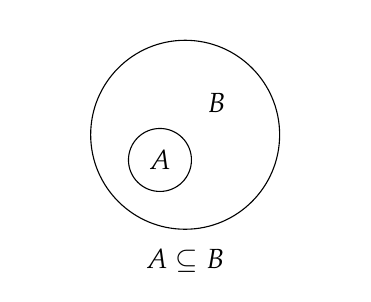
\begin{tikzpicture}[scale=0.8]
                    \tkzInit[xmin=-2.5,xmax=2.5,ymin=-2.2,ymax=1.7]
                    \tkzClip

                    \draw (0,0) circle (1.5);
                    \node at(0.5,0.5) {$B$};
    
                    \tkzDefPoint(-0.4,-0.4){A}
                    \draw (A) circle (0.5);
                    \node at(A) {$A$};
    
                    \node at(0,-2.0) {$A\subseteq B$};
                \end{tikzpicture}
            }
            \subfigure
            {
                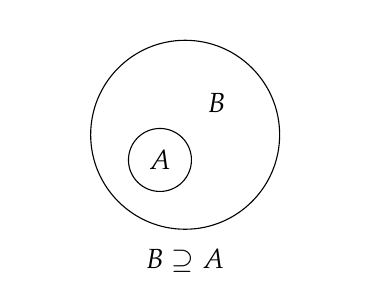
\begin{tikzpicture}[scale=0.8]
                    \tkzInit[xmin=-2.5,xmax=2.5,ymin=-2.2,ymax=1.7]
                    \tkzClip

                    \draw (0,0) circle (1.5);
                    \node at(0.5,0.5) {$B$};
    
                    \tkzDefPoint(-0.4,-0.4){A}
                    \draw (A) circle (0.5);
                    \node at(A) {$A$};
    
                    \node at(0,-2.0) {$B\supseteq A$};
                \end{tikzpicture}
            }
            \caption{集合和集合的关系}
        \end{center}
    \end{figure}\\
    由此形象的使用文氏图表现了集合和集合的关系。

\newpage

\subsubsection{交集运算}
    由属于集合$A$且属于集合$B$的元素组成的集合,称为集合$A$与集合$B$的交集。\\[3mm]
    集合$A$和集合$B$的交集的数学表达:
    \begin{large}
        \begin{equation*}
            A\cap B=\big\{ x\mid x\in A~\text{且}~x\in B\big\}
        \end{equation*}
    \end{large}\\
    集合$A$和集合$B$的交集的文氏图表达:
    \begin{figure}[h]
        \begin{center}
            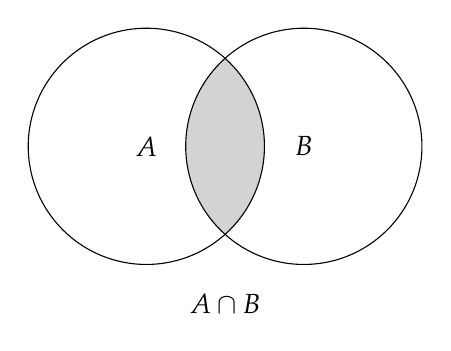
\begin{tikzpicture}
                \begin{scope}
                    \clip (-1,0) circle (1.5);
                    \clip (+1,0) circle (1.5);
                    \fill[LightGray] (-1,0) circle (1.5);
                    \fill[LightGray] (+1,0) circle (1.5);
                \end{scope}
                \draw (-1,0) circle (1.5);
                \draw (+1,0) circle (1.5);
                \node at(-1,0) {$A$};
                \node at(+1,0) {$B$};
                \node at(0,-2) {$A\cap B$};
            \end{tikzpicture}
            \caption{交集的文氏图表达}
        \end{center}
    \end{figure}\\
    集合的交集运算有以下重要性质:
    \begin{large}
        \begin{align*}
            &A\cap B=B\cap A\\[3mm]
            &A\cap A=A\\[3mm]
            &A\cap \emptyset=\emptyset\\[3mm]
            &A\cap B\subseteq A\\[3mm]
            &A\cap B\subseteq B
        \end{align*}
    \end{large}\\
    此外多个集合的交集也可以表示为:
    \begin{large}
        \begin{equation*}
            \bigcap_{i=1}^{n}A_n=A_1\cap A_2\cap\cdots\cap A_n
        \end{equation*}
    \end{large}\\
    这个符号代表$A_1\sim A_n$共计$n$个集合依次取交集。

\newpage

\subsubsection{并集运算}
    由属于集合$A$或属于集合$B$的元素组成的集合,称为集合$A$与集合$B$的并集。\\[3mm]
    集合$A$和集合$B$的并集的文氏图表达:
    \begin{large}
        \begin{equation*}
            A\cup B=\big\{ x\mid x\in A~\text{或}~x\in B\big\}
        \end{equation*}
    \end{large}\\
    集合$A$和集合$B$的并集的文氏图表达:
    \begin{figure}[h]
        \begin{center}
            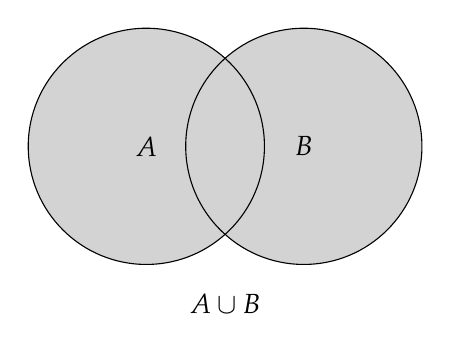
\begin{tikzpicture}
                \fill[LightGray] (-1,0) circle (1.5);
                \fill[LightGray] (+1,0) circle (1.5);
                \draw (-1,0) circle (1.5);
                \draw (+1,0) circle (1.5);
                \node at(-1,0) {$A$};
                \node at(+1,0) {$B$};
                \node at(0,-2) {$A\cup B$};
            \end{tikzpicture}
            \caption{并集的文氏图表达}
        \end{center}
    \end{figure}\\
    集合的并集运算有以下重要性质:
    \begin{large}
        \begin{align*}
            &A\cup B=B\cup A\\[3mm]
            &A\cup A=A\\[3mm]
            &A\cup \emptyset=A\\[3mm]
            &A\cup B\supseteq A\\[3mm]
            &A\cup B\supseteq B
        \end{align*}
    \end{large}\\
    此外多个集合的并集也可以表示为:
    \begin{large}
        \begin{equation*}
            \bigcup_{i=1}^{n}A_n=A_1\cup A_2\cup\cdots\cup A_n
        \end{equation*}
    \end{large}\\
    这个符号代表$A_1\sim A_n$共计$n$个集合依次取并集。

\newpage

\subsubsection{集合的性质$1$}
    集合的性质$1$的基本形式:
    \begin{large}
        \begin{equation*}
            A\cup(B\cap C)=(A\cup B)\cap(A\cup C)
        \end{equation*}
    \end{large}\\
    集合的性质$1$的推广形式:
    \begin{large}
        \begin{equation*}
            A\cup\left(\bigcap_{i=1}^n B_i\right)=\bigcap_{i=1}^n(A\cup B_i)
        \end{equation*}
    \end{large}\\[5mm]
    基本形式的等式左侧可以用文氏图表示为:\vspace{5pt}
    \begin{figure}[h!]
        \begin{center}
            \subfigure
            {
                \begin{minipage}[t]{0.23\linewidth}
                    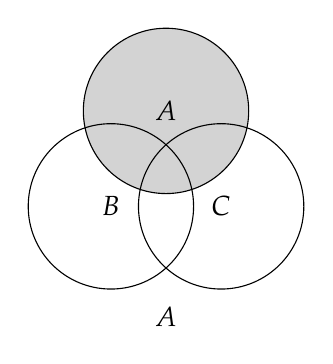
\begin{tikzpicture}[scale=0.7]
                        \fill[LightGray] (0,1.732) circle (1.5);
                        \draw (0,1.732) circle (1.5);
                        \draw (-1,0) circle (1.5);
                        \draw (+1,0) circle (1.5);
                        \node at(0,1.732) {$A$};
                        \node at(-1,0) {$B$};
                        \node at(+1,0) {$C$};
                        \node at(0,-2) {$A$};
                    \end{tikzpicture}
                \end{minipage}
            }\qquad
            \subfigure
            {
                \begin{minipage}[t]{0.23\linewidth}
                    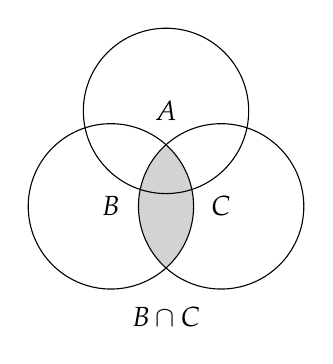
\begin{tikzpicture}[scale=0.7]
                        \begin{scope}
                            \clip (-1,0) circle (1.5);
                            \clip (+1,0) circle (1.5);
                            \fill[LightGray] (-1,0) circle (1.5);
                            \fill[LightGray] (+1,0) circle (1.5);
                        \end{scope}
                        \draw (0,1.732) circle (1.5);
                        \draw (-1,0) circle (1.5);
                        \draw (+1,0) circle (1.5);
                        \node at(0,1.732) {$A$};
                        \node at(-1,0) {$B$};
                        \node at(+1,0) {$C$};
                        \node at(0,-2) {$B\cap C$};
                    \end{tikzpicture}
                \end{minipage}
            }\qquad
            \subfigure
            {
                \begin{minipage}[t]{0.23\linewidth}
                    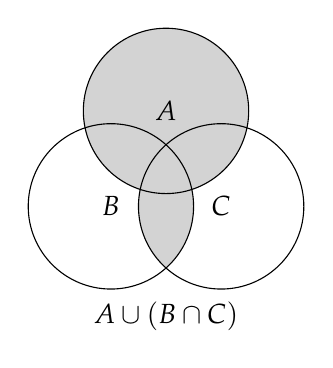
\begin{tikzpicture}[scale=0.7]
                        \begin{scope}
                            \clip (-1,0) circle (1.5);
                            \clip (+1,0) circle (1.5);
                            \fill[LightGray] (-1,0) circle (1.5);
                            \fill[LightGray] (+1,0) circle (1.5);
                        \end{scope}
                        \fill[LightGray] (0,1.732) circle (1.5);
                        \draw (0,1.732) circle (1.5);
                        \draw (-1,0) circle (1.5);
                        \draw (+1,0) circle (1.5);
                        \node at(0,1.732) {$A$};
                        \node at(-1,0) {$B$};
                        \node at(+1,0) {$C$};
                        \node at(0,-2) {$A\cup(B\cap C)$};
                    \end{tikzpicture}
                \end{minipage}
            }
            \caption{等式左侧的文氏图表达}
        \end{center}
    \end{figure}\\
    基本形式的等式右侧可以用文氏图表示为:\vspace{5pt}
    \begin{figure}[h!]
        \begin{center}
            \subfigure
            {
                \begin{minipage}[t]{0.23\linewidth}
                    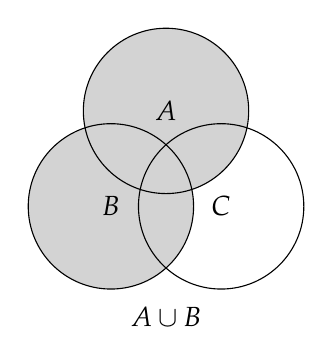
\begin{tikzpicture}[scale=0.7]
                        \fill[LightGray] (0,1.732) circle (1.5);
                        \fill[LightGray] (-1,0) circle (1.5);
                        \draw (0,1.732) circle (1.5);
                        \draw (-1,0) circle (1.5);
                        \draw (+1,0) circle (1.5);
                        \node at(0,1.732) {$A$};
                        \node at(-1,0) {$B$};
                        \node at(+1,0) {$C$};
                        \node at(0,-2) {$A\cup B$};
                    \end{tikzpicture}
                \end{minipage}
            }\qquad
            \subfigure
            {
                \begin{minipage}[t]{0.23\linewidth}
                    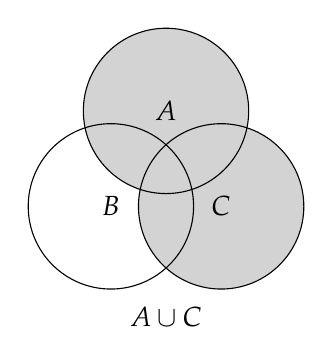
\begin{tikzpicture}[scale=0.7]
                        \fill[LightGray] (0,1.732) circle (1.5);
                        \fill[LightGray] (+1,0) circle (1.5);
                        \draw (0,1.732) circle (1.5);
                        \draw (-1,0) circle (1.5);
                        \draw (+1,0) circle (1.5);
                        \node at(0,1.732) {$A$};
                        \node at(-1,0) {$B$};
                        \node at(+1,0) {$C$};
                        \node at(0,-2) {$A\cup C$};
                    \end{tikzpicture}
                \end{minipage}
            }\qquad
            \subfigure
            {
                \begin{minipage}[t]{0.23\linewidth}
                    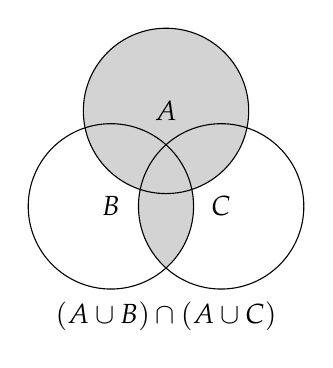
\begin{tikzpicture}[scale=0.7]
                        \begin{scope}
                            \clip (-1,0) circle (1.5);
                            \clip (+1,0) circle (1.5);
                            \fill[LightGray] (-1,0) circle (1.5);
                            \fill[LightGray] (+1,0) circle (1.5);
                        \end{scope}
                        \fill[LightGray] (0,1.732) circle (1.5);
                        \draw (0,1.732) circle (1.5);
                        \draw (-1,0) circle (1.5);
                        \draw (+1,0) circle (1.5);
                        \node at(0,1.732) {$A$};
                        \node at(-1,0) {$B$};
                        \node at(+1,0) {$C$};
                        \node at(0,-2) {$(A\cup B)\cap (A\cup C)$};
                    \end{tikzpicture}
                \end{minipage}
            }
            \caption{等式右侧的文氏图表达}
        \end{center}
    \end{figure}\\
    由两组文氏图可以看出,最终得出的结论是一致的,因此基本形式由此证明。

\newpage

    推广形式可以使用第一类数学归纳法加以证明。\\[3mm]
    假设以下式子成立:
    \setcounter{equation}{0}
    \begin{align}
        A\cup\left(\bigcap_{i=1}^n B_i\right)=\bigcap_{i=1}^n(A\cup B_i)
    \end{align}\\
    我们进行以下代换:
    \begin{align}
        B_1=C_1~~,~~B_2=C_2~~,~~\cdots~~,~~B_{n-1}=C_{n-1}~~,~~B_n=C_n\cap C_{n+1}
    \end{align}\\
    左式既可以表示为:
    \begin{align}
        A\cup\left(\bigcap_{i=1}^n B_i\right)=A\cup\left(\bigcap_{i=1}^{n+1} C_i\right)~~~~~~~~~~~~~~~~~~~~~~~
    \end{align}\\
    左式也可以表示为:
    \begin{align}
        &~~~~~~~~~~~~~~~~~~~~A\cup\left(\bigcap_{i=1}^n B_i\right)=\bigcap_{i=1}^n(A\cup B_i)\\[3mm]
        &~~~~~~~~~~~~~~~~~~~~A\cup\left(\bigcap_{i=1}^n B_i\right)=\left[\bigcap_{i=1}^{n-1}(A\cup B_i)\right]\cap(A\cup B_n)\\[3mm]
        &~~~~~~~~~~~~~~~~~~~~A\cup\left(\bigcap_{i=1}^n B_i\right)=\left[\bigcap_{i=1}^{n-1}(A\cup C_i)\right]\cap(A\cup (C_n\cap C_{n+1}))\\[3mm]
        &~~~~~~~~~~~~~~~~~~~~A\cup\left(\bigcap_{i=1}^n B_i\right)=\left[\bigcap_{i=1}^{n-1}(A\cup C_i)\right]\cap(A\cup C_n)\cap(A\cup C_{n+1})\\[3mm]
        &~~~~~~~~~~~~~~~~~~~~A\cup\left(\bigcap_{i=1}^n B_i\right)=\bigcap_{i=1}^{n+1}(A\cup C_i)
    \end{align}\\
    联立两个结论可得:
    \begin{align}
        A\cup\left(\bigcap_{i=1}^{n+1} C_i\right)=\bigcap_{i=1}^{n+1}(A\cup C_i)
    \end{align}\\
    由此证明了该假设可以由$n\Rightarrow n+1$,然而已经证明该假设在$n=2$时成立,因此假设成立。

\newpage

\subsubsection{集合的性质$2$}
    集合的性质$2$的基本形式:
    \begin{large}
        \begin{equation*}
            A\cap(B\cup C)=(A\cap B)\cup(A\cap C)
        \end{equation*}
    \end{large}\\
    集合的性质$2$的推广形式:
    \begin{large}
        \begin{equation*}
            A\cap\left(\bigcup_{i=1}^n B_i\right)=\bigcup_{i=1}^n(A\cap B_i)
        \end{equation*}
    \end{large}\\[5mm]
    基本形式的等式左侧可以用文氏图表示为:\vspace{5pt}
    \begin{figure}[h!]
        \begin{center}
            \subfigure
            {
                \begin{minipage}[t]{0.23\linewidth}
                    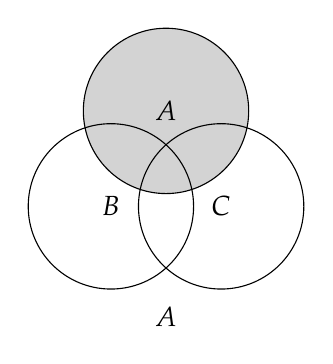
\begin{tikzpicture}[scale=0.7]
                        \fill[LightGray] (0,1.732) circle (1.5);
                        \draw (0,1.732) circle (1.5);
                        \draw (-1,0) circle (1.5);
                        \draw (+1,0) circle (1.5);
                        \node at(0,1.732) {$A$};
                        \node at(-1,0) {$B$};
                        \node at(+1,0) {$C$};
                        \node at(0,-2) {$A$};
                    \end{tikzpicture}
                \end{minipage}
            }\qquad
            \subfigure
            {
                \begin{minipage}[t]{0.23\linewidth}
                    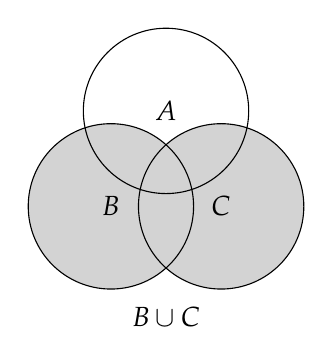
\begin{tikzpicture}[scale=0.7]
                        \fill[LightGray] (-1,0) circle (1.5);
                        \fill[LightGray] (+1,0) circle (1.5);
                        \draw (0,1.732) circle (1.5);
                        \draw (-1,0) circle (1.5);
                        \draw (+1,0) circle (1.5);
                        \node at(0,1.732) {$A$};
                        \node at(-1,0) {$B$};
                        \node at(+1,0) {$C$};
                        \node at(0,-2) {$B\cup C$};
                    \end{tikzpicture}
                \end{minipage}
            }\qquad
            \subfigure
            {
                \begin{minipage}[t]{0.23\linewidth}
                    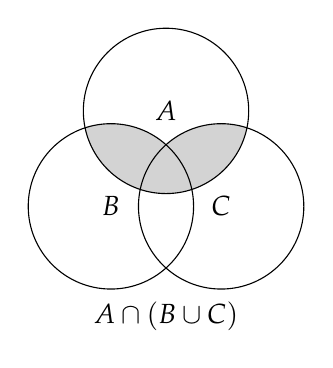
\begin{tikzpicture}[scale=0.7]
                        \begin{scope}
                            \clip (0,1.732) circle (1.5);
                            \fill[LightGray] (-1,0) circle (1.5);
                            \fill[LightGray] (+1,0) circle (1.5);
                        \end{scope}
                        \draw (0,1.732) circle (1.5);
                        \draw (-1,0) circle (1.5);
                        \draw (+1,0) circle (1.5);
                        \node at(0,1.732) {$A$};
                        \node at(-1,0) {$B$};
                        \node at(+1,0) {$C$};
                        \node at(0,-2) {$A\cap(B\cup C)$};
                    \end{tikzpicture}
                \end{minipage}
            }
            \caption{等式左侧的文氏图表达}
        \end{center}
    \end{figure}\\
    基本形式的等式右侧可以用文氏图表示为:\vspace{5pt}
    \begin{figure}[h!]
        \begin{center}
            \subfigure
            {
                \begin{minipage}[t]{0.23\linewidth}
                    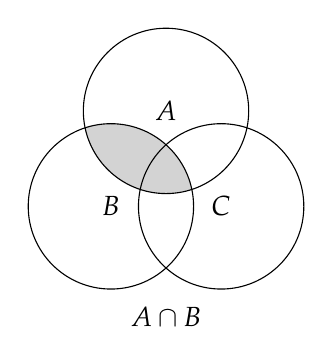
\begin{tikzpicture}[scale=0.7]
                        \begin{scope}
                            \clip (0,1.732) circle (1.5);
                            \clip (-1,0) circle (1.5);
                            \fill[LightGray] (0,1.732) circle (1.5);
                            \fill[LightGray] (-1,0) circle (1.5);
                        \end{scope}
                        \draw (0,1.732) circle (1.5);
                        \draw (-1,0) circle (1.5);
                        \draw (+1,0) circle (1.5);
                        \node at(0,1.732) {$A$};
                        \node at(-1,0) {$B$};
                        \node at(+1,0) {$C$};
                        \node at(0,-2) {$A\cap B$};
                    \end{tikzpicture}
                \end{minipage}
            }\qquad
            \subfigure
            {
                \begin{minipage}[t]{0.23\linewidth}
                    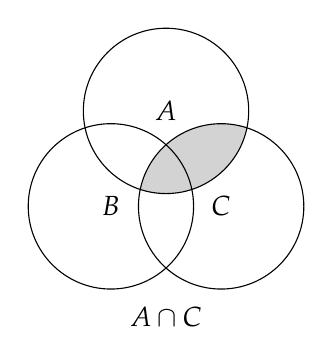
\begin{tikzpicture}[scale=0.7]
                        \begin{scope}
                            \clip (0,1.732) circle (1.5);
                            \clip (+1,0) circle (1.5);
                            \fill[LightGray] (0,1.732) circle (1.5);
                            \fill[LightGray] (-1,0) circle (1.5);
                        \end{scope}
                        \draw (0,1.732) circle (1.5);
                        \draw (-1,0) circle (1.5);
                        \draw (+1,0) circle (1.5);
                        \node at(0,1.732) {$A$};
                        \node at(-1,0) {$B$};
                        \node at(+1,0) {$C$};
                        \node at(0,-2) {$A\cap C$};
                    \end{tikzpicture}
                \end{minipage}
            }\qquad
            \subfigure
            {
                \begin{minipage}[t]{0.23\linewidth}
                    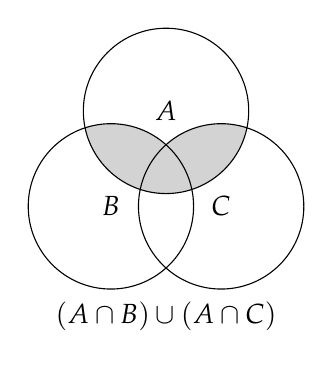
\begin{tikzpicture}[scale=0.7]
                        \begin{scope}
                            \clip (0,1.732) circle (1.5);
                            \fill[LightGray] (-1,0) circle (1.5);
                            \fill[LightGray] (+1,0) circle (1.5);
                        \end{scope}
                        \draw (0,1.732) circle (1.5);
                        \draw (-1,0) circle (1.5);
                        \draw (+1,0) circle (1.5);
                        \node at(0,1.732) {$A$};
                        \node at(-1,0) {$B$};
                        \node at(+1,0) {$C$};
                        \node at(0,-2) {$(A\cap B)\cup (A\cap C)$};
                    \end{tikzpicture}
                \end{minipage}
            }
            \caption{等式右侧的文氏图表达}
        \end{center}
    \end{figure}\\
    由两组文氏图可以看出,最终得出的结论是一致的,因此基本形式由此证明。

\newpage

    推广形式可以使用第一类数学归纳法加以证明。\\[3mm]
    假设以下式子成立:
    \setcounter{equation}{0}
    \begin{align}
        A\cap\left(\bigcup_{i=1}^n B_i\right)=\bigcup_{i=1}^n(A\cap B_i)
    \end{align}\\
    我们进行以下代换:
    \begin{align}
        B_1=C_1~~,~~B_2=C_2~~,~~\cdots~~,~~B_{n-1}=C_{n-1}~~,~~B_n=C_n\cup C_{n+1}
    \end{align}\\
    左式既可以表示为:
    \begin{align}
        A\cap\left(\bigcup_{i=1}^n B_i\right)=A\cap\left(\bigcup_{i=1}^{n+1} C_i\right)~~~~~~~~~~~~~~~~~~~~~~~
    \end{align}\\
    左式也可以表示为:
    \begin{align}
        &~~~~~~~~~~~~~~~~~~~~A\cap\left(\bigcup_{i=1}^n B_i\right)=\bigcup_{i=1}^n(A\cap B_i)\\[3mm]
        &~~~~~~~~~~~~~~~~~~~~A\cap\left(\bigcup_{i=1}^n B_i\right)=\left[\bigcup_{i=1}^{n-1}(A\cap B_i)\right]\cup(A\cap B_n)\\[3mm]
        &~~~~~~~~~~~~~~~~~~~~A\cap\left(\bigcup_{i=1}^n B_i\right)=\left[\bigcup_{i=1}^{n-1}(A\cap C_i)\right]\cup(A\cap (C_n\cup C_{n+1}))\\[3mm]
        &~~~~~~~~~~~~~~~~~~~~A\cap\left(\bigcup_{i=1}^n B_i\right)=\left[\bigcup_{i=1}^{n-1}(A\cap C_i)\right]\cup(A\cap C_n)\cup(A\cap C_{n+1})\\[3mm]
        &~~~~~~~~~~~~~~~~~~~~A\cap\left(\bigcup_{i=1}^n B_i\right)=\bigcup_{i=1}^{n+1}(A\cap C_i)
    \end{align}\\
    联立两个结论可得:
    \begin{align}
        A\cap\left(\bigcup_{i=1}^{n+1} C_i\right)=\bigcup_{i=1}^{n+1}(A\cap C_i)
    \end{align}\\
    由此证明了该假设可以由$n\Rightarrow n+1$,然而已经证明该假设在$n=2$时成立,因此假设成立。

\newpage

\subsubsection{补集运算}
    由属于集合$U$且不属于集合$A$的元素组成的集合,称为集合$A$在集合$U$中的补集。\\[3mm]
    需要指出的是,集合$U$应当满足为集合$A$的超集,集合$A$应当满足为集合$U$的子集。\\[3mm]
    需要说明的是,集合$U$在补集运算中,通常被称为全集。\\[4mm]
    集合$A$在集合$U$中的补集的数学表达:
    \begin{large}
        \begin{equation*}
            \complement_UA=\big\{ x\mid x\in U~\text{且}~x\notin A\big\}
        \end{equation*}
    \end{large}\\
    集合$A$在集合$U$中的补集的文氏图表达:\vspace{3pt}
    \begin{figure}[h]
        \begin{center}
            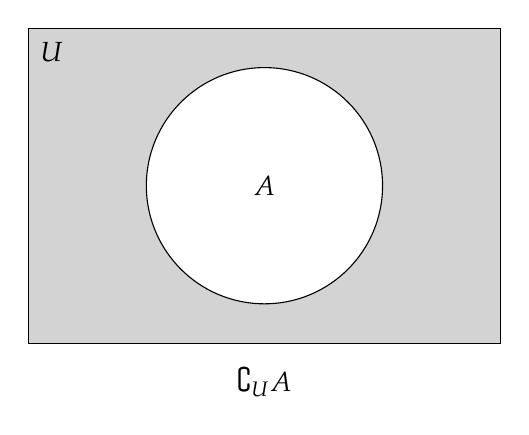
\begin{tikzpicture}
                \fill[LightGray] (-3,+2.0) rectangle (+3,-2.0);
                \fill[white] (0,0) circle (1.5);

                \draw (-3,+2.0) rectangle (+3,-2.0);
                \draw (0,0) circle (1.5);
                
                \node at(0,0) {$A$};
                \node at(0,-2.5) {$\complement_U A$};

                \node at(-2.7,+1.7) {$U$};
            \end{tikzpicture}
            \caption{补集的文氏图表达}
        \end{center}
    \end{figure}\\
    集合的补集运算有以下重要性质:
    \begin{large}
        \begin{align*}
            &\complement_UA\cap A=\emptyset\\[6mm]
            &\complement_UA\cup A=U\\[6mm]
            &\complement_U\big[\complement_UA\big]=A
        \end{align*}
    \end{large}\\
    补集运算中的运算符$\complement$为一特殊符号,不可以用$C$代替。

\newpage

\subsubsection{集合的性质$3$}
    集合的性质$3$的基本形式:
    \begin{large}
        \begin{equation*}
            \complement_UA\cap\complement_UB=\complement_U\left(A\cup B\right)
        \end{equation*}
    \end{large}\\
    集合的性质$3$的推广形式:
    \begin{large}
        \begin{equation*}
            \bigcap_{i=1}^n \complement_UA_i=\complement_U\left(\bigcup_{i=1}^n A_i\right)
        \end{equation*}
    \end{large}\\[5mm]
    基本形式的等式左侧可以用文氏图表示为:\vspace{5pt}
    \begin{figure}[h!]
        \begin{center}
            \subfigure
            {
                \begin{minipage}[t]{0.27\linewidth}
                    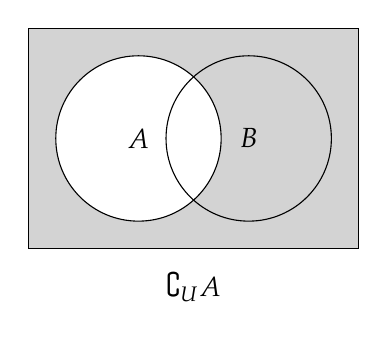
\begin{tikzpicture}[scale=0.7]
                        \fill[LightGray] (-3,+2) rectangle (+3,-2);
                        \fill[white] (-1,0) circle (1.5);
                        \draw (-3,+2) rectangle (+3,-2);
                        \draw (-1,0) circle (1.5);
                        \draw (+1,0) circle (1.5);
                        \node at(-1,0) {$A$};
                        \node at(+1,0) {$B$};
                        \node at(0,-2.7) {$\complement_U A$};
                    \end{tikzpicture}
                \end{minipage}
            }\quad
            \subfigure
            {
                \begin{minipage}[t]{0.27\linewidth}
                    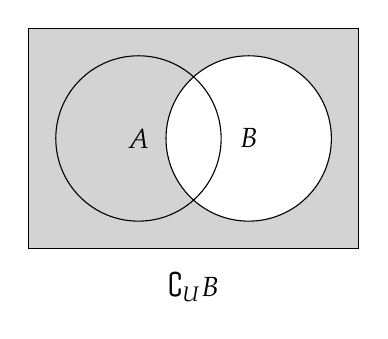
\begin{tikzpicture}[scale=0.7]
                        \fill[LightGray] (-3,+2) rectangle (+3,-2);
                        \fill[white] (+1,0) circle (1.5);
                        \draw (-3,+2) rectangle (+3,-2);
                        \draw (-1,0) circle (1.5);
                        \draw (+1,0) circle (1.5);
                        \node at(-1,0) {$A$};
                        \node at(+1,0) {$B$};
                        \node at(0,-2.7) {$\complement_U B$};
                    \end{tikzpicture}
                \end{minipage}
            }\quad
            \subfigure
            {
                \begin{minipage}[t]{0.27\linewidth}
                    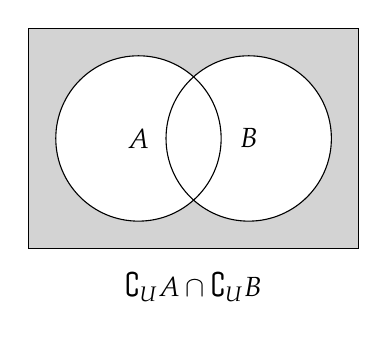
\begin{tikzpicture}[scale=0.7]
                        \fill[LightGray] (-3,+2) rectangle (+3,-2);
                        \fill[white] (-1,0) circle (1.5);
                        \fill[white] (+1,0) circle (1.5);
                        \draw (-3,+2) rectangle (+3,-2);
                        \draw (-1,0) circle (1.5);
                        \draw (+1,0) circle (1.5);
                        \node at(-1,0) {$A$};
                        \node at(+1,0) {$B$};
                        \node at(0,-2.7) {$\complement_UA\cap\complement_UB$};
                    \end{tikzpicture}
                \end{minipage}
            }
            \caption{等式左侧的文氏图表达}
        \end{center}
    \end{figure}\\
    基本形式的等式右侧可以用文氏图表示为:\vspace{5pt}
    \begin{figure}[h!]
        \begin{center}
            \subfigure
            {
                \begin{minipage}[t]{0.27\linewidth}
                    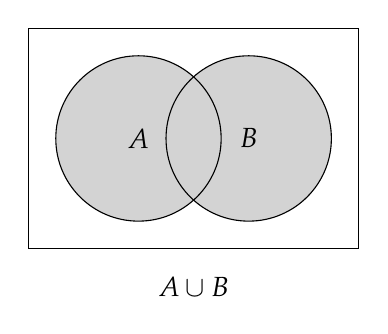
\begin{tikzpicture}[scale=0.7]
                        \fill[LightGray] (-1,0) circle (1.5);
                        \fill[LightGray] (+1,0) circle (1.5);
                        \draw (-3,+2) rectangle (+3,-2);
                        \draw (-1,0) circle (1.5);
                        \draw (+1,0) circle (1.5);
                        \node at(-1,0) {$A$};
                        \node at(+1,0) {$B$};
                        \node at(0,-2.7) {$A\cup B$};
                    \end{tikzpicture}
                \end{minipage}
            }\quad
            \subfigure
            {
                \begin{minipage}[t]{0.27\linewidth}
                    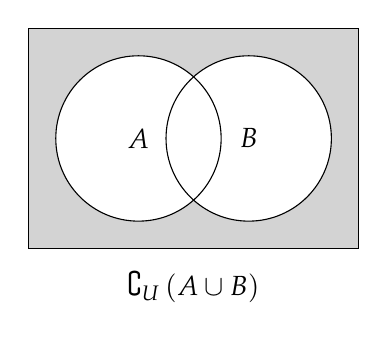
\begin{tikzpicture}[scale=0.7]
                        \fill[LightGray] (-3,+2) rectangle (+3,-2);
                        \fill[white] (-1,0) circle (1.5);
                        \fill[white] (+1,0) circle (1.5);
                        \draw (-3,+2) rectangle (+3,-2);
                        \draw (-1,0) circle (1.5);
                        \draw (+1,0) circle (1.5);
                        \node at(-1,0) {$A$};
                        \node at(+1,0) {$B$};
                        \node at(0,-2.7) {$\complement_U\left(A\cup B\right)$};
                    \end{tikzpicture}
                \end{minipage}
            }
            \caption{等式左侧的文氏图表达}
        \end{center}
    \end{figure}\\
    由两组文氏图可以看出,最终得出的结论是一致的,因此基本形式由此证明。

\newpage

    推广形式可以使用第一类数学归纳法加以证明。\\[3mm]
    假设以下式子成立:
    \setcounter{equation}{0}
    \begin{align}
        \bigcap_{i=1}^n \complement_UB_i=\complement_U\left(\bigcup_{i=1}^n B_i\right)
    \end{align}\\
    我们进行以下代换:
    \begin{align}
        B_1=C_1~~,~~B_2=C_2~~,~~\cdots~~,~~B_{n-1}=C_{n-1}~~,~~B_n=C_n\cup C_{n+1}
    \end{align}\\
    右式既可以表示为:
    \begin{align}
        \complement_U\left(\bigcup_{i=1}^n B_i\right)=\complement_U\left(\bigcap_{i=1}^{n+1}Ci\right)~~~~~~~~~~~~~~
    \end{align}\\
    右式也可以表示为:
    \begin{align}
        &~~~~~~~~~~~~~~\complement_U\left(\bigcup_{i=1}^n B_i\right)=\bigcap_{i=1}^n\complement_U B_i\\[3mm]
        &~~~~~~~~~~~~~~\complement_U\left(\bigcup_{i=1}^n B_i\right)=\left(\bigcap_{i=1}^{n-1}\complement_U B_i\right)\cap\complement_U B_n\\[3mm]
        &~~~~~~~~~~~~~~\complement_U\left(\bigcup_{i=1}^n B_i\right)=\left(\bigcap_{i=1}^{n-1}\complement_U C_i\right)\cap\complement_U\left(C_n\cup C_{n+1}\right)\\[3mm]
        &~~~~~~~~~~~~~~\complement_U\left(\bigcup_{i=1}^n B_i\right)=\left(\bigcap_{i=1}^{n-1}\complement_U C_i\right)\cap\complement_UC_n\cap \complement_UC_{n+1}\\[3mm]
        &~~~~~~~~~~~~~~\complement_U\left(\bigcup_{i=1}^n B_i\right)=\bigcap_{i=1}^{n+1}\complement_U C_i
    \end{align}\\
    联立两个结论可得:
    \begin{align}
        \bigcap_{i=1}^{n+1} \complement_UC_i=\complement_U\left(\bigcup_{i=1}^{n+1} C_i\right)
    \end{align}\\
    由此证明了该假设可以由$n\Rightarrow n+1$,然而已经证明该假设在$n=2$时成立,因此假设成立。

\newpage

\subsubsection{集合的性质$4$}
    集合的性质$4$的基本形式:
    \begin{large}
        \begin{equation*}
            \complement_UA\cup\complement_UB=\complement_U\left(A\cap B\right)
        \end{equation*}
    \end{large}\\
    集合的性质$4$的推广形式:
    \begin{large}
        \begin{equation*}
            \bigcup_{i=1}^n \complement_UA_i=\complement_U\left(\bigcap_{i=1}^n A_i\right)
        \end{equation*}
    \end{large}\\[5mm]
    基本形式的等式左侧可以用文氏图表示为:\vspace{5pt}
    \begin{figure}[h!]
        \begin{center}
            \subfigure
            {
                \begin{minipage}[t]{0.27\linewidth}
                    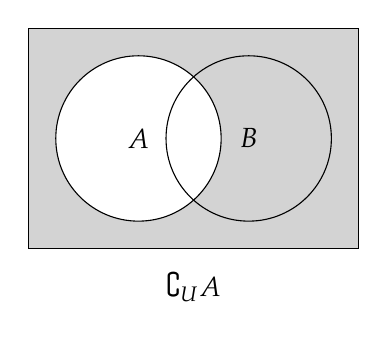
\begin{tikzpicture}[scale=0.7]
                        \fill[LightGray] (-3,+2) rectangle (+3,-2);
                        \fill[white] (-1,0) circle (1.5);
                        \draw (-3,+2) rectangle (+3,-2);
                        \draw (-1,0) circle (1.5);
                        \draw (+1,0) circle (1.5);
                        \node at(-1,0) {$A$};
                        \node at(+1,0) {$B$};
                        \node at(0,-2.7) {$\complement_U A$};
                    \end{tikzpicture}
                \end{minipage}
            }\quad
            \subfigure
            {
                \begin{minipage}[t]{0.27\linewidth}
                    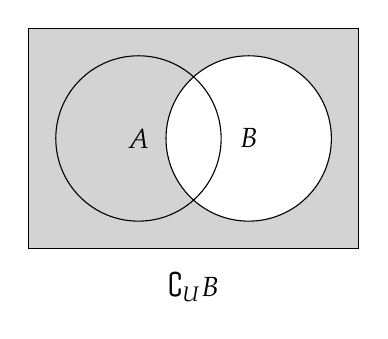
\begin{tikzpicture}[scale=0.7]
                        \fill[LightGray] (-3,+2) rectangle (+3,-2);
                        \fill[white] (+1,0) circle (1.5);
                        \draw (-3,+2) rectangle (+3,-2);
                        \draw (-1,0) circle (1.5);
                        \draw (+1,0) circle (1.5);
                        \node at(-1,0) {$A$};
                        \node at(+1,0) {$B$};
                        \node at(0,-2.7) {$\complement_U B$};
                    \end{tikzpicture}
                \end{minipage}
            }\quad
            \subfigure
            {
                \begin{minipage}[t]{0.27\linewidth}
                    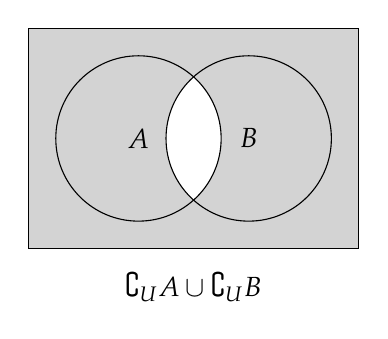
\begin{tikzpicture}[scale=0.7]
                        \fill[LightGray] (-3,+2) rectangle (+3,-2);
                        \begin{scope}
                            \clip (-1,0) circle (1.5);
                            \clip (+1,0) circle (1.5);
                            \fill[white] (-1,0) circle (1.5);
                            \fill[white] (+1,0) circle (1.5);
                        \end{scope}
                        \draw (-3,+2) rectangle (+3,-2);
                        \draw (-1,0) circle (1.5);
                        \draw (+1,0) circle (1.5);
                        \node at(-1,0) {$A$};
                        \node at(+1,0) {$B$};
                        \node at(0,-2.7) {$\complement_UA\cup\complement_UB$};
                    \end{tikzpicture}
                \end{minipage}
            }
            \caption{等式左侧的文氏图表达}
        \end{center}
    \end{figure}\\
    基本形式的等式右侧可以用文氏图表示为:\vspace{5pt}
    \begin{figure}[h!]
        \begin{center}
            \subfigure
            {
                \begin{minipage}[t]{0.27\linewidth}
                    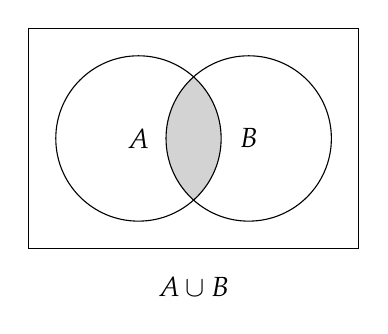
\begin{tikzpicture}[scale=0.7]
                        \begin{scope}
                            \clip (-1,0) circle (1.5);
                            \clip (+1,0) circle (1.5);
                            \fill[LightGray] (-1,0) circle (1.5);
                            \fill[LightGray] (+1,0) circle (1.5);
                        \end{scope}
                        \draw (-3,+2) rectangle (+3,-2);
                        \draw (-1,0) circle (1.5);
                        \draw (+1,0) circle (1.5);
                        \node at(-1,0) {$A$};
                        \node at(+1,0) {$B$};
                        \node at(0,-2.7) {$A\cup B$};
                    \end{tikzpicture}
                \end{minipage}
            }\quad
            \subfigure
            {
                \begin{minipage}[t]{0.27\linewidth}
                    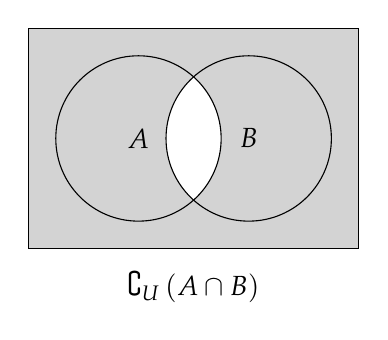
\begin{tikzpicture}[scale=0.7]
                        \fill[LightGray] (-3,+2) rectangle (+3,-2);
                        \begin{scope}
                            \clip (-1,0) circle (1.5);
                            \clip (+1,0) circle (1.5);
                            \fill[white] (-1,0) circle (1.5);
                            \fill[white] (+1,0) circle (1.5);
                        \end{scope}
                        \draw (-3,+2) rectangle (+3,-2);
                        \draw (-1,0) circle (1.5);
                        \draw (+1,0) circle (1.5);
                        \node at(-1,0) {$A$};
                        \node at(+1,0) {$B$};
                        \node at(0,-2.7) {$\complement_U\left(A\cap B\right)$};
                    \end{tikzpicture}
                \end{minipage}
            }
            \caption{等式左侧的文氏图表达}
        \end{center}
    \end{figure}\\
    由两组文氏图可以看出,最终得出的结论是一致的,因此基本形式由此证明。

\newpage

    推广形式可以使用第一类数学归纳法加以证明。\\[3mm]
    假设以下式子成立:
    \setcounter{equation}{0}
    \begin{align}
        \bigcup_{i=1}^n \complement_UB_i=\complement_U\left(\bigcap_{i=1}^n B_i\right)
    \end{align}\\
    我们进行以下代换:
    \begin{align}
        B_1=C_1~~,~~B_2=C_2~~,~~\cdots~~,~~B_{n-1}=C_{n-1}~~,~~B_n=C_n\cap C_{n+1}
    \end{align}\\
    右式既可以表示为:
    \begin{align}
        \complement_U\left(\bigcap_{i=1}^n B_i\right)=\complement_U\left(\bigcup_{i=1}^{n+1}Ci\right)~~~~~~~~~~~~~~
    \end{align}\\
    右式也可以表示为:
    \begin{align}
        &~~~~~~~~~~~~~~\complement_U\left(\bigcap_{i=1}^n B_i\right)=\bigcup_{i=1}^n\complement_U B_i\\[3mm]
        &~~~~~~~~~~~~~~\complement_U\left(\bigcap_{i=1}^n B_i\right)=\left(\bigcup_{i=1}^{n-1}\complement_U B_i\right)\cup\complement_U B_n\\[3mm]
        &~~~~~~~~~~~~~~\complement_U\left(\bigcap_{i=1}^n B_i\right)=\left(\bigcup_{i=1}^{n-1}\complement_U C_i\right)\cup\complement_U\left(C_n\cap C_{n+1}\right)\\[3mm]
        &~~~~~~~~~~~~~~\complement_U\left(\bigcap_{i=1}^n B_i\right)=\left(\bigcup_{i=1}^{n-1}\complement_U C_i\right)\cup\complement_UC_n\cup \complement_UC_{n+1}\\[3mm]
        &~~~~~~~~~~~~~~\complement_U\left(\bigcap_{i=1}^n B_i\right)=\bigcup_{i=1}^{n+1}\complement_U C_i
    \end{align}\\
    联立两个结论可得:
    \begin{align}
        \bigcup_{i=1}^{n+1} \complement_UC_i=\complement_U\left(\bigcap_{i=1}^{n+1} C_i\right)
    \end{align}\\
    由此证明了该假设可以由$n\Rightarrow n+1$,然而已经证明该假设在$n=2$时成立,因此假设成立。

\newpage

\subsubsection{数集的区间表示}
    数集也可以使用区间进行简便的表示,假设$a,b\in\mathbb{R}$且满足$a<b$。\\[3mm]
    以下数集可以用区间表示,称为闭区间:
    \begin{large}
        \begin{equation*}
            \left\{x~|~a\leq x\leq b\right\}=[a,b]
        \end{equation*}
    \end{large}\\
    以下数集可以用区间表示,称为开区间:
    \begin{large}
        \begin{equation*}
            \left\{x~|~a<x<b\right\}=(a,b)
        \end{equation*}
    \end{large}\\
    以下数集可以用区间表示,称为左闭右开区间:
    \begin{large}
        \begin{equation*}
            \left\{x~|~a\leq x<b\right\}=[a,b)
        \end{equation*}
    \end{large}\\
    以下数集可以用区间表示,称为左开右闭区间:
    \begin{large}
        \begin{equation*}
            \left\{x~|~a\leq x<b\right\}=(a,b]
        \end{equation*}
    \end{large}\\
    区间可以在数轴上表示:
    \begin{figure}[h]
        \begin{center}
            \subfigure[闭区间]
            {
                \begin{tikzpicture}
                    \tkzDefPoint(0,0){O}
                    \tkzDefPoint(-2.5,0){X1}
                    \tkzDefPoint(+2.5,0){X2}
                    \tkzDrawSegment[->](X1,X2)
                    \tkzLabelPoint[above](X2){$x$}

                    \tkzDefPoint(-1.2,0){A}
                    \tkzDefPoint(+1.2,0){B}

                    \tkzDefShiftPoint[A](0,0.5){A1}
                    \tkzDefShiftPoint[B](0,0.5){B1}

                    \tkzDrawSegments(A,A1 B,B1 A1,B1)
                    \tkzDrawPoints[fill=black](A,B)

                    \tkzLabelPoint[below=2pt](A){$a$}
                    \tkzLabelPoint[below](B){$b$}
                    
                    \tkzLabelPoint[above=14pt](O){$[a,b]$}
                \end{tikzpicture}
            }\qquad\qquad
            \subfigure[开区间]
            {
                \begin{tikzpicture}
                    \tkzDefPoint(0,0){O}
                    \tkzDefPoint(-2.5,0){X1}
                    \tkzDefPoint(+2.5,0){X2}
                    \tkzDrawSegment[->](X1,X2)
                    \tkzLabelPoint[above](X2){$x$}

                    \tkzDefPoint(-1.2,0){A}
                    \tkzDefPoint(+1.2,0){B}

                    \tkzDefShiftPoint[A](0,0.5){A1}
                    \tkzDefShiftPoint[B](0,0.5){B1}

                    \tkzDrawSegments(A,A1 B,B1 A1,B1)
                    \tkzDrawPoints[fill=white](A,B)

                    \tkzLabelPoint[below=2pt](A){$a$}
                    \tkzLabelPoint[below](B){$b$}
                    
                    \tkzLabelPoint[above=14pt](O){$(a,b)$}
                \end{tikzpicture}
            }\\[5mm]
            \subfigure[左闭右开区间]
            {
                \begin{tikzpicture}
                    \tkzDefPoint(0,0){O}
                    \tkzDefPoint(-2.5,0){X1}
                    \tkzDefPoint(+2.5,0){X2}
                    \tkzDrawSegment[->](X1,X2)
                    \tkzLabelPoint[above](X2){$x$}

                    \tkzDefPoint(-1.2,0){A}
                    \tkzDefPoint(+1.2,0){B}

                    \tkzDefShiftPoint[A](0,0.5){A1}
                    \tkzDefShiftPoint[B](0,0.5){B1}

                    \tkzDrawSegments(A,A1 B,B1 A1,B1)
                    \tkzDrawPoints[fill=black](A)
                    \tkzDrawPoints[fill=white](B)

                    \tkzLabelPoint[below=2pt](A){$a$}
                    \tkzLabelPoint[below](B){$b$}
                    
                    \tkzLabelPoint[above=14pt](O){$[a,b)$}
                \end{tikzpicture}
            }\qquad\qquad
            \subfigure[左开右闭区间]
            {
                \begin{tikzpicture}
                    \tkzDefPoint(0,0){O}
                    \tkzDefPoint(-2.5,0){X1}
                    \tkzDefPoint(+2.5,0){X2}
                    \tkzDrawSegment[->](X1,X2)
                    \tkzLabelPoint[above](X2){$x$}

                    \tkzDefPoint(-1.2,0){A}
                    \tkzDefPoint(+1.2,0){B}

                    \tkzDefShiftPoint[A](0,0.5){A1}
                    \tkzDefShiftPoint[B](0,0.5){B1}

                    \tkzDrawSegments(A,A1 B,B1 A1,B1)
                    \tkzDrawPoints[fill=white](A)
                    \tkzDrawPoints[fill=black](B)

                    \tkzLabelPoint[below=2pt](A){$a$}
                    \tkzLabelPoint[below](B){$b$}
                    
                    \tkzLabelPoint[above=14pt](O){$(a,b]$}
                \end{tikzpicture}
            }
            \caption{区间在数轴上的表示}
        \end{center}
    \end{figure}\\
    区间可以分为有限区间和无限区间,上述列出的都是有限区间。\\[3mm]
    无限区间中包含$\big\{x~|~x\geq a\big\}=[a,+\infty)$以及$\big\{x~|~x>a\big\}=(a,+\infty)$,其中$+\infty$称为正无穷大。\\[3mm]
    无限区间中包含$\big\{x~|~x\leq b\big\}=(-\infty,b]$以及$\big\{x~|~x<b\big\}=(-\infty,b)$,其中$-\infty$称为负无穷大。\\[3mm]

\newpage

\subsection{命题}
    命题的通常形式:如果$\alpha$,那么$\beta$。\\[3mm]
    命题中的$\alpha$和$\beta$是两个事件,事件$\alpha$称为条件,事件$\beta$称为结论。\\[3mm]
    若事件$\alpha$可以推出事件$\beta$,那么这个命题是真命题:
    \begin{large}
        \begin{equation*}
            \alpha~\Longrightarrow~\beta
        \end{equation*}
    \end{large}\\
    若事件$\alpha$不能推出事件$\beta$,那么这个命题是假命题:
    \begin{large}
        \begin{equation*}
            \alpha~\not\Longrightarrow~\beta
        \end{equation*}
    \end{large}\vspace{-15pt}

\subsubsection{命题的四种形式}
    命题的四种形式的意义:\vspace{3pt}
    \begin{table}[h!]
        \begin{center}
            \begin{tabular}{p{70pt}|p{70pt}|p{170pt}}
                \hline
                原命题&$\alpha\Rightarrow\beta$&若事件$\alpha$为真,则事件$\beta$为真。\\ \hline
                否命题&$\bar{\alpha}\Rightarrow\bar{\beta}$&若事件$\alpha$为假,则事件$\beta$为假。\\ \hline
                逆命题&$\beta\Rightarrow\alpha$&若事件$\beta$为真,则事件$\alpha$为真。\\ \hline
                逆否命题&$\bar{\beta}\Rightarrow\bar{\alpha}$&若事件$\beta$为假,则事件$\alpha$为假。\\ \hline
            \end{tabular}
            \caption{命题的四种形式的意义}
        \end{center}
    \end{table}\\
    命题的四种形式的关系:\vspace{5pt}
    \begin{figure}[h!]
        \begin{center}
            \begin{tikzpicture}[scale=1.0]
                \foreach \a/\x/\y in{1/-4/+1.5,2/-4/-1.5,3/+4/+1.5,4/+4/-1.5}
                {
                    \tkzDefPoint(\x,\y){R\a}

                    \tkzDefShiftPoint[R\a](-1.2,-0.6){RR1\a}
                    \tkzDefShiftPoint[R\a](+1.2,+0.6){RR2\a}

                    \tkzDefShiftPoint[R\a](-1.2,0){R\a L}
                    \tkzDefShiftPoint[R\a](+1.2,0){R\a R}
                    \tkzDefShiftPoint[R\a](0,-0.6){R\a D}
                    \tkzDefShiftPoint[R\a](0,+0.6){R\a U}

                    \tkzDefShiftPoint[R\a](-1.2,+0.6){R\a UL}
                    \tkzDefShiftPoint[R\a](+1.2,+0.6){R\a UR}
                    \tkzDefShiftPoint[R\a](-1.2,-0.6){R\a DL}
                    \tkzDefShiftPoint[R\a](+1.2,-0.6){R\a DR}

                    \draw[thick] (RR1\a) rectangle (RR2\a);
                }

                \tkzDefPoint(0,0){O}

                \tkzLabelPoint[below](R1){$\alpha\Rightarrow\beta$}
                \tkzLabelPoint[below](R2){$\bar{\alpha}\Rightarrow\bar{\beta}$}
                \tkzLabelPoint[below](R3){$\beta\Rightarrow\alpha$}
                \tkzLabelPoint[below](R4){$\bar{\beta}\Rightarrow\bar{\alpha}$}

                \tkzLabelPoint[above](R1){\small 原命题}
                \tkzLabelPoint[above](R2){\small 否命题}
                \tkzLabelPoint[above](R3){\small 逆命题}
                \tkzLabelPoint[above](R4){\small 逆否命题}

                \tkzDrawSegments[<->](R1R,R3L R2R,R4L R1D,R2U R3D,R4U R1DR,R4UL R2UR,R3DL)

                \tkzLabelSegment[above](R1R,R3L){\small 互~~逆}
                \tkzLabelSegment[below](R2R,R4L){\small 互~~逆}

                \tkzLabelSegment[left,text width=1em](R1D,R2U){\small 互否}
                \tkzLabelSegment[right,text width=1em](R3D,R4U){\small 互否}

                \tkzLabelPoint[above=5pt](O){\small 互~~逆~~否}
                \tkzLabelPoint[below=5pt](O){\small 互~~逆~~否}
            \end{tikzpicture}
        \end{center}
        \caption{命题的四种形式的关系}
    \end{figure}\\
    在上方的表格和示意图中,事件$\bar{\alpha}$指的是事件$\alpha$的否定\\[3mm]
    在上方的表格和示意图中,事件$\bar{\beta}$指的是事件$\beta$的否定。\\[3mm]
    原命题和逆否命题同时为真或同时为假,即两者互为等价命题。

\newpage

\subsubsection{命题中的充分条件和必要条件}
    \setcounter{equation}{0}
    对于这样一个命题$\alpha\Rightarrow\beta$:\\[3mm]
    我们将事件$\alpha$称为事件$\beta$的充分条件,充分条件代表“有它即可”。\\[3mm]
    我们将事件$\beta$称为事件$\alpha$的必要条件,必要条件代表“无它不可”。\\[6mm]
    由于原命题$\alpha\Rightarrow\beta$成立,因此逆否命题$\bar{\beta}\Rightarrow\bar{\alpha}$成立:\\[3mm]
    充分条件的含义:因为$\alpha\Rightarrow\beta$,若有条件$\alpha$,那么事件$\beta$必然成立,因此$\alpha$对$\beta$是充分的。\\[3mm]
    必要条件的含义:因为$\bar{\beta}\Rightarrow\bar{\alpha}$,若无条件$\beta$,那么事件$\alpha$不能成立,因此$\beta$对$\alpha$是必要的。\\[6mm]
    如果事件$\alpha$和事件$\beta$满足:
    \begin{align}
        \alpha~\Longrightarrow~\beta
    \end{align}\\
    同时事件$\alpha$和事件$\beta$满足:
    \begin{align}
        \beta~\Longrightarrow~\alpha
    \end{align}\\
    根据第一个命题$\alpha\Rightarrow\beta$可知,此时$\alpha$为$\beta$的充分条件,同时$\beta$为$\alpha$的必要条件。\\[3mm]
    根据第二个命题$\beta\Rightarrow\alpha$可知,此时$\alpha$为$\beta$的必要条件,同时$\beta$为$\alpha$的充分条件。\\[3mm]
    此时事件$\alpha$和事件$\beta$的关系记作:
    \begin{large}
        \begin{equation*}
            \alpha~\Longleftrightarrow~\beta
        \end{equation*}
    \end{large}\\
    此时认为事件$\alpha$和事件$\beta$等价,两者互为充要条件。\vspace{5pt}

\subsubsection{命题中的子集关系与推出关系}
    \setcounter{equation}{0}
    对于非空集合$A$:
    \begin{equation}
        A=\big\{a~|~\text{元素}a\text{具有性质}\alpha\big\}
    \end{equation}\\
    对于非空集合$B$:
    \begin{equation}
        B=\big\{b~|~\text{元素}b\text{具有性质}\beta\big\}
    \end{equation}\\
    此时子集关系$A\subseteq B$等价于推出关系$\alpha\Rightarrow\beta$,故$\alpha$为$\beta$的充分条件,而$\beta$为$\alpha$的必要条件。\\[3mm]
    该性质称为子集与推出关系,也可以简单的概括为“以小推大”。
    

\newpage

\section{不等式}

\subsection{不等式的性质}
    两个实数的大小可以通过其差和零的比较确定。\\[3mm]
    两个实数的大小关系的充要条件:
    \begin{large}
        \begin{equation*}
            \begin{cases}
                ~a>b~~~~\Longleftrightarrow~~~~a-b>0\\[1mm]
                ~a=b~~~~\Longleftrightarrow~~~~a-b=0\\[1mm]
                ~a<b~~~~\Longleftrightarrow~~~~a-b<0\\
            \end{cases}
        \end{equation*}
    \end{large}

\subsubsection{不等式的对称性}
    \setcounter{equation}{0}
    不等式的对称性:
    \begin{large}
        \begin{equation*}
            a>b~~~~\Longleftrightarrow~~~~b<a
        \end{equation*}
    \end{large}\\
    根据实数大小关系的充要条件:
    \begin{align}
        a>b~~~~\Longleftrightarrow~~~~a-b>0\\[3mm]
        b<a~~~~\Longleftrightarrow~~~~b-a<0
    \end{align}\\
    由于正数$a-b$的相反数$b-a$为负数,因此有$a-b>0\Longrightarrow b-a<0$成立。\vspace{8pt}

\subsubsection{不等式的传递性}
    \setcounter{equation}{0}
    不等式的传递性:
    \begin{large}
        \begin{equation*}
            \begin{cases}
                ~a>b\\[1mm]
                ~b>c\\
            \end{cases}\Longrightarrow~~~~a>c
        \end{equation*}
    \end{large}\\
    根据实数大小关系的充要条件:
    \begin{align}
        a>b~~~~\Longleftrightarrow~~~~a-b>0\\[3mm]
        b>c~~~~\Longleftrightarrow~~~~b-c>0
    \end{align}\\
    由于正数$a-b$和正数$b-c$的和仍为正数,故$(a-b)+(b-c)>0$成立,即$a-c>0$成立。\\[3mm]
    由实数的大小关系的充要条件可知,由$a-c>0$可以推出$a>c$。

\newpage

\subsubsection{不等式的可加性}
    \setcounter{equation}{0}
    不等式的可加性指出,不等式的两侧加上相同的实数,不等式的符号方向不变。\\[3mm]
    不等式的可加性:
    \begin{large}
        \begin{equation*}
            \begin{cases}
                ~a>b\\[3mm]
                ~a,b\in\mathbb{R}~~~~\lambda\in\mathbb{R}\\
            \end{cases}
            \Longrightarrow~~~~\lambda+a>\lambda+b
        \end{equation*}
    \end{large}\\[3mm]
    不等式的可加性的示意图:
    \begin{figure}[h]
        \begin{center}
            \begin{tikzpicture}[scale=1.0]
                \tkzInit[xmin=-4.3,xmax=+4.3,ymin=-4.3,ymax=+4.3]
                \tkzClip

                \tkzDefPoint(0,0){O}

                \tkzDefShiftPoint[O](-4,0){X1}
                \tkzDefShiftPoint[O](+4,0){X2}

                \tkzDefShiftPoint[O](0,-4){Y1}
                \tkzDefShiftPoint[O](0,+4){Y2}

                \tkzDrawSegment[->](X1,X2)
                \tkzDrawSegment[->](Y1,Y2)

                \tkzLabelPoint[above](X2){$x$}
                \tkzLabelPoint[right](Y2){$y$}

                \tkzDefPoint(0,1){L1}
                \tkzDefPoint(1,2){L2}

                \tkzDrawSegment[color=LiGreen2,thick,add=2.5 and 1.0](L1,L2)

                \tkzDefPoint(0.75,0){b}
                \tkzDefPoint(1.50,0){a}

                \tkzDefLine[orthogonal=through a](X1,X2)
                \tkzGetPoint{a'}

                \tkzInterLL(a,a')(L1,L2)
                \tkzGetPoint{A}

                \tkzDefLine[orthogonal=through b](X1,X2)
                \tkzGetPoint{b'}

                \tkzInterLL(b,b')(L1,L2)
                \tkzGetPoint{B}

                \tkzDrawSegments[dashed](A,a B,b)
                \tkzDrawPoints[fill=white](A,B,a,b,O)

                \tkzLabelPoint[below=2.5pt](a){$a$}
                \tkzLabelPoint[below](b){$b$}

                \tkzDefShiftPoint[Y1](0,0.4){f}
                \tkzLabelPoint[right=2pt](f){$y=x+\lambda$};
            \end{tikzpicture}
            \caption{不等式的可加性}
        \end{center}
    \end{figure}\\
    构造函数$y=x+\lambda$并绘制函数图像,观察到在$a>b$时总有$a+\lambda>b+\lambda$。\\[3mm]
    根据实数大小关系的充要条件:
    \begin{align}
        a>b~~~~\Longrightarrow~~~~a-b>0
    \end{align}\\
    由于$a-b$与$a+\lambda-b-\lambda$相等:
    \begin{align}
        &~a+\lambda-b-\lambda>0\\[4mm]
        &(a+\lambda)-(b+\lambda)>0~~~~\Longrightarrow~~~~a+\lambda>b+\lambda
    \end{align}\\
    由此严格的证明了不等式的可加性。

\newpage

\subsubsection{不等式的正可乘性}
    \setcounter{equation}{0}
    不等式的正可乘性指出,不等式的两侧乘上相同的正数,不等式的符号方向不变。\\[3mm]
    不等式的正可乘性:
    \begin{large}
        \begin{align*}
            \begin{cases}
                ~a>b\\[3mm]
                ~a,b\in\mathbb{R}~~~~\lambda\in\mathbb{R^+}\\
            \end{cases}
            \Longrightarrow~~~~\lambda\cdot a>\lambda\cdot b
        \end{align*}
    \end{large}\\[3mm]
    不等式的正可乘性的示意图:
    \begin{figure}[h]
        \begin{center}
            \begin{tikzpicture}[scale=1.0]
                \tkzInit[xmin=-4.3,xmax=+4.3,ymin=-4.3,ymax=+4.3]
                \tkzClip

                \tkzDefPoint(0,0){O}

                \tkzDefShiftPoint[O](-4,0){X1}
                \tkzDefShiftPoint[O](+4,0){X2}

                \tkzDefShiftPoint[O](0,-4){Y1}
                \tkzDefShiftPoint[O](0,+4){Y2}

                \tkzDrawSegment[->](X1,X2)
                \tkzDrawSegment[->](Y1,Y2)

                \tkzLabelPoint[above](X2){$x$}
                \tkzLabelPoint[right](Y2){$y$}

                \tkzDefPoint(-1,-1.5){L1}
                \tkzDefPoint(+1,+1.5){L2}

                \tkzDrawSegment[color=LiGreen2,thick,add=0.5 and 0.5](L1,L2)

                \tkzDefPoint(0.75,0){b}
                \tkzDefPoint(1.50,0){a}

                \tkzDefLine[orthogonal=through a](X1,X2)
                \tkzGetPoint{a'}

                \tkzInterLL(a,a')(L1,L2)
                \tkzGetPoint{A}

                \tkzDefLine[orthogonal=through b](X1,X2)
                \tkzGetPoint{b'}

                \tkzInterLL(b,b')(L1,L2)
                \tkzGetPoint{B}

                \tkzDrawSegments[dashed](A,a B,b)
                \tkzDrawPoints[fill=white](A,B,a,b,O)

                \tkzLabelPoint[below=2.5pt](a){$a$}
                \tkzLabelPoint[below](b){$b$}

                \tkzDefShiftPoint[Y1](0,0.4){f}
                \tkzLabelPoint[right=2pt](f){$y=\lambda\cdot x~~(\lambda>0)$};
            \end{tikzpicture}
            \caption{不等式的正可乘性}
        \end{center}
    \end{figure}\\
    构造函数$y=\lambda\cdot x~~(\lambda>0)$并绘制函数图像,观察到在$a>b$时总有$\lambda\cdot a>\lambda\cdot b$。\\[3mm]
    根据实数大小关系的充要条件:
    \begin{align}
        a>b~~~~\Longrightarrow~~~~a-b>0
    \end{align}\\
    正数$a-b$和正数$\lambda$的积仍为正数:\vspace{3pt}
    \begin{align}
        &\lambda\cdot(a-b)>0\\[3mm]
        &\lambda\cdot a-\lambda\cdot b>0~~~~\Longrightarrow~~~~\lambda\cdot a>\lambda\cdot b
    \end{align}\\
    由此严格的证明了不等式的正可乘性。

\newpage

\subsubsection{不等式的负可乘性}
    \setcounter{equation}{0}
    不等式的负可乘性指出,不等式的两侧乘上相同的负数,不等式的符号方向改变。\\[3mm]
    不等式的负可乘性:
    \begin{large}
        \begin{align*}
            \begin{cases}
                ~a>b\\[3mm]
                ~a,b\in\mathbb{R}~~~~\lambda\in\mathbb{R^-}\\
            \end{cases}
            \Longrightarrow~~~~\lambda\cdot a<\lambda\cdot b
        \end{align*}
    \end{large}\\[3mm]
    不等式的负可乘性的示意图:
    \begin{figure}[h]
        \begin{center}
            \begin{tikzpicture}[scale=1.0]
                \tkzInit[xmin=-4.3,xmax=+4.3,ymin=-4.3,ymax=+4.3]
                \tkzClip

                \tkzDefPoint(0,0){O}

                \tkzDefShiftPoint[O](-4,0){X1}
                \tkzDefShiftPoint[O](+4,0){X2}

                \tkzDefShiftPoint[O](0,-4){Y1}
                \tkzDefShiftPoint[O](0,+4){Y2}

                \tkzDrawSegment[->](X1,X2)
                \tkzDrawSegment[->](Y1,Y2)

                \tkzLabelPoint[above](X2){$x$}
                \tkzLabelPoint[right](Y2){$y$}

                \tkzDefPoint(+1,-1.5){L1}
                \tkzDefPoint(-1,+1.5){L2}

                \tkzDrawSegment[color=LiGreen2,thick,add=0.5 and 0.5](L1,L2)

                \tkzDefPoint(0.75,0){b}
                \tkzDefPoint(1.50,0){a}

                \tkzDefLine[orthogonal=through a](X1,X2)
                \tkzGetPoint{a'}

                \tkzInterLL(a,a')(L1,L2)
                \tkzGetPoint{A}

                \tkzDefLine[orthogonal=through b](X1,X2)
                \tkzGetPoint{b'}

                \tkzInterLL(b,b')(L1,L2)
                \tkzGetPoint{B}

                \tkzDrawSegments[dashed](A,a B,b)
                \tkzDrawPoints[fill=white](A,B,a,b,O)

                \tkzLabelPoint[above](a){$a$}
                \tkzLabelPoint[above](b){$b$}

                \tkzDefShiftPoint[Y1](0,0.4){f}
                \tkzLabelPoint[right=2pt](f){$y=\lambda\cdot x~~(\lambda<0)$};
            \end{tikzpicture}
            \caption{不等式的负可乘性}
        \end{center}
    \end{figure}\\
    构造函数$y=\lambda\cdot x~~(\lambda<0)$并绘制函数图像,观察到在$a>b$时总有$\lambda\cdot a<\lambda\cdot b$。\\[3mm]
    根据实数大小关系的充要条件:
    \begin{align}
        a>b~~~~\Longrightarrow~~~~a-b>0
    \end{align}\\
    正数$a-b$和负数$\lambda$的积变为负数:\vspace{3pt}
    \begin{align}
        &\lambda\cdot(a-b)<0\\[3mm]
        &\lambda\cdot a-\lambda\cdot b<0~~~~\Longrightarrow~~~~\lambda\cdot a<\lambda\cdot b
    \end{align}\\
    由此严格的证明了不等式的负可乘性。

\newpage

    \subsubsection{不等式的倒数法则}
    不等式的倒数法则指出,不等式在两侧同号时取倒数,所得不等式的符号方向不变。\\[3mm]
    不等式的倒数法则:
    \begin{large}
        \begin{align*}
            &\begin{cases}
                ~a>b\\[3mm]
                ~ab>0~~~~a,b\in\mathbb{R}
            \end{cases}
            \Longrightarrow~~~~\frac{1}{a}<\frac{1}{b}
        \end{align*}
    \end{large}\\
    不等式的倒数法则的示意图:
    \begin{figure}[h]
        \begin{center}
            \begin{tikzpicture}[scale=1.0]
                \tkzInit[xmin=-4.3,xmax=+4.3,ymin=-4.3,ymax=+4.3]
                \tkzClip

                \tkzDefPoint(0,0){O}

                \tkzDefShiftPoint[O](-4,0){X1}
                \tkzDefShiftPoint[O](+4,0){X2}

                \tkzDefShiftPoint[O](0,-4){Y1}
                \tkzDefShiftPoint[O](0,+4){Y2}

                \tkzDrawSegment[->](X1,X2)
                \tkzDrawSegment[->](Y1,Y2)

                \tkzLabelPoint[above](X2){$x$}
                \tkzLabelPoint[right](Y2){$y$}

                \draw[color=LiGreen2,smooth,thick,samples=100,domain=+0.3:+3.3] plot(\x,{1/\x});
                \draw[color=LiGreen2,smooth,thick,samples=100,domain=-3.3:-0.3] plot(\x,{1/\x});

                \tkzDefPoint(-0.50,0){b1}
                \tkzDefPoint(-1.50,0){a1}

                \tkzDefPoint(-0.50,-2.00){B1}
                \tkzDefPoint(-1.50,-0.66){A1}

                \tkzDefPoint(0.50,0){b2}
                \tkzDefPoint(1.50,0){a2}

                \tkzDefPoint(0.50,2.00){B2}
                \tkzDefPoint(1.50,0.66){A2}

                \tkzDrawSegments[dashed](A1,a1 B1,b1 A2,a2 B2,b2)
                \tkzDrawPoints[fill=white](A1,B1,a1,b1,A2,B2,a2,b2,O)

                \tkzLabelPoint[above](a1){$b$}
                \tkzLabelPoint[above](b1){$a$}

                \tkzLabelPoint[below=2.5pt](a2){$a$}
                \tkzLabelPoint[below](b2){$b$}

                \tkzDefShiftPoint[Y1](0,0.7){f}
                \tkzLabelPoint[right=2pt](f){$y=\dfrac{1}{x}$};
            \end{tikzpicture}
            \caption{不等式的倒数法则}
        \end{center}
    \end{figure}\\
    构造函数$y=\dfrac{1}{x}$并绘制函数图像,观察到在正半轴中$a>b$时总有$\dfrac{1}{a}<\dfrac{1}{b}$。\\[4mm]
    构造函数$y=\dfrac{1}{x}$并绘制函数图像,观察到在负半轴中$a>b$时总有$\dfrac{1}{a}<\dfrac{1}{b}$。\\[5mm]
    由此通过图像论证了不等式的倒数法则。

\newpage

\subsubsection{不等式的乘法法则}    
    不等式的乘方法则指出,不等式在两侧均为正时乘方,所得不等式的符号方向不变。\\[3mm]
    不等式的乘方法则:
    \begin{large}
        \begin{align*}
            &\begin{cases}
                ~a>b\\[3mm]
                ~a,b\in\mathbb{R^+}~~~~n\in\mathbb{Z^+}
            \end{cases}
            \Longrightarrow~~~~a^n>b^n
        \end{align*}
    \end{large}\\[3mm]
    不等式的乘方法则的示意图:
    \begin{figure}[h]
        \begin{center}
            \subfigure[当$n$为偶数的情况]
            {
                \begin{tikzpicture}[scale=0.8]
                    \tkzInit[xmin=-4.3,xmax=+4.3,ymin=-4.3,ymax=+4.3]
                    \tkzClip
    
                    \tkzDefPoint(0,0){O}
    
                    \tkzDefShiftPoint[O](-4,0){X1}
                    \tkzDefShiftPoint[O](+4,0){X2}
    
                    \tkzDefShiftPoint[O](0,-4){Y1}
                    \tkzDefShiftPoint[O](0,+4){Y2}
    
                    \tkzDrawSegment[->](X1,X2)
                    \tkzDrawSegment[->](Y1,Y2)
    
                    \tkzLabelPoint[above](X2){$x$}
                    \tkzLabelPoint[right](Y2){$y$}
    
                    \draw[color=LiGreen2,smooth,thick,samples=100,domain=-1.8:0] plot(\x,{\x*\x});
                    \draw[color=LiGreen2,smooth,thick,samples=100,domain=0:+1.8] plot(\x,{\x*\x});
    
                    \tkzDefPoint(0.75,0){b}
                    \tkzDefPoint(1.50,0){a}
    
                    \tkzDefPoint(0.75,0.56){B}
                    \tkzDefPoint(1.50,2.25){A}
    
                    \tkzDrawSegments[dashed](A,a B,b)
                    \tkzDrawPoints[fill=white](A,a,B,b,O)
    
                    \tkzLabelPoint[below=2.5pt](a){$a$}
                    \tkzLabelPoint[below](b){$b$}
    
                    \tkzDefShiftPoint[Y1](0,0.7){f}
                    \tkzLabelPoint[right=2pt](f){$y=x^n$};
                \end{tikzpicture}
            }\qquad
            \subfigure[当$n$为奇数的情况]
            {
                \begin{tikzpicture}[scale=0.8]
                    \tkzInit[xmin=-4.3,xmax=+4.3,ymin=-4.3,ymax=+4.3]
                    \tkzClip
    
                    \tkzDefPoint(0,0){O}
    
                    \tkzDefShiftPoint[O](-4,0){X1}
                    \tkzDefShiftPoint[O](+4,0){X2}
    
                    \tkzDefShiftPoint[O](0,-4){Y1}
                    \tkzDefShiftPoint[O](0,+4){Y2}
    
                    \tkzDrawSegment[->](X1,X2)
                    \tkzDrawSegment[->](Y1,Y2)
    
                    \tkzLabelPoint[above](X2){$x$}
                    \tkzLabelPoint[right](Y2){$y$}
    
                    \draw[color=LiGreen2,smooth,thick,samples=100,domain=-1.55:0] plot(\x,{\x*\x*\x});
                    \draw[color=LiGreen2,smooth,thick,samples=100,domain=0:+1.55] plot(\x,{\x*\x*\x});
    
                    \tkzDefPoint(0.75,0){b}
                    \tkzDefPoint(1.50,0){a}
    
                    \tkzDefPoint(0.75,0.42){B}
                    \tkzDefPoint(1.50,3.375){A}
    
                    \tkzDrawSegments[dashed](A,a B,b)
                    \tkzDrawPoints[fill=white](A,a,B,b,O)
    
                    \tkzLabelPoint[below=2.5pt](a){$a$}
                    \tkzLabelPoint[below](b){$b$}
    
                    \tkzDefShiftPoint[Y1](0,0.7){f}
                    \tkzLabelPoint[right=2pt](f){$y=x^n$};
                \end{tikzpicture}
            }
            \caption{不等式的乘方法则}
        \end{center}
    \end{figure}\\
    构造函数$y=x^n$并绘制函数图像,当$n$为偶数时观察到在正半轴中$a>b$时总有$a^n>b^n$。\\[3mm]
    构造函数$y=x^n$并绘制函数图像,当$n$为奇数时观察到在正半轴中$a>b$时总有$a^n>b^n$。\\[3mm]
    由此通过图像论证了不等式的乘方法则。

\newpage

\subsubsection{不等式的开方法则}
    不等式的开方法则指出,不等式在两侧均为正时开方,所得不等式的符号方向不变。\\[3mm]
    不等式的开方法则:
    \begin{large}
        \begin{align*}
            \begin{cases}
                ~a>b\\[3mm]
                ~a,b\in\mathbb{R^+}~~~~n\in\mathbb{Z^+}
            \end{cases}
            \Longrightarrow~~~~\sqrt[n]{\vphantom{b}a}>\sqrt[n]{b}
        \end{align*}
    \end{large}\\[3mm]
    不等式的开方法则的示意图:
    \begin{figure}[h]
        \begin{center}
            \subfigure[当$n$为偶数的情况]
            {
                \begin{tikzpicture}[scale=0.8]
                    \tkzInit[xmin=-4.3,xmax=+4.3,ymin=-4.3,ymax=+4.3]
                    \tkzClip
    
                    \tkzDefPoint(0,0){O}
    
                    \tkzDefShiftPoint[O](-4,0){X1}
                    \tkzDefShiftPoint[O](+4,0){X2}
    
                    \tkzDefShiftPoint[O](0,-4){Y1}
                    \tkzDefShiftPoint[O](0,+4){Y2}
    
                    \tkzDrawSegment[->](X1,X2)
                    \tkzDrawSegment[->](Y1,Y2)
    
                    \tkzLabelPoint[above](X2){$x$}
                    \tkzLabelPoint[right](Y2){$y$}
    
                    \draw[color=LiGreen2,smooth,thick,samples=100,domain=0:3.5] plot(\x,{\x^0.5});
    
                    \tkzDefPoint(1.00,0){b}
                    \tkzDefPoint(2.50,0){a}
    
                    \tkzDefPoint(1.00,1.00){B}
                    \tkzDefPoint(2.50,1.58){A}
    
                    \tkzDrawSegments[dashed](A,a B,b)
                    \tkzDrawPoints[fill=white](A,a,B,b,O)
    
                    \tkzLabelPoint[below=2.5pt](a){$a$}
                    \tkzLabelPoint[below](b){$b$}
    
                    \tkzDefShiftPoint[Y1](0,0.7){f}
                    \tkzLabelPoint[right=2pt](f){$y=\sqrt[n]{x}$};
                \end{tikzpicture}
            }\qquad
            \subfigure[当$n$为奇数的情况]
            {
                \begin{tikzpicture}[scale=0.8]
                    \tkzInit[xmin=-4.3,xmax=+4.3,ymin=-4.3,ymax=+4.3]
                    \tkzClip
    
                    \tkzDefPoint(0,0){O}
    
                    \tkzDefShiftPoint[O](-4,0){X1}
                    \tkzDefShiftPoint[O](+4,0){X2}
    
                    \tkzDefShiftPoint[O](0,-4){Y1}
                    \tkzDefShiftPoint[O](0,+4){Y2}
    
                    \tkzDrawSegment[->](X1,X2)
                    \tkzDrawSegment[->](Y1,Y2)
    
                    \tkzLabelPoint[above](X2){$x$}
                    \tkzLabelPoint[right](Y2){$y$}
    
                    \draw[color=LiGreen2,smooth,thick,samples=100,domain=-3.5:+3.5] plot(\x,{\x^0.333});
    
                    \tkzDefPoint(1.00,0){b}
                    \tkzDefPoint(2.50,0){a}
    
                    \tkzDefPoint(1.00,1.00){B}
                    \tkzDefPoint(2.50,1.36){A}
    
                    \tkzDrawSegments[dashed](A,a B,b)
                    \tkzDrawPoints[fill=white](A,a,B,b,O)
    
                    \tkzLabelPoint[below=2.5pt](a){$a$}
                    \tkzLabelPoint[below](b){$b$}
    
                    \tkzDefShiftPoint[Y1](0,0.7){f}
                    \tkzLabelPoint[right=2pt](f){$y=\sqrt[n]{x}$};;
                \end{tikzpicture}
            }
            \caption{不等式的开方法则}
        \end{center}
    \end{figure}\\
    构造函数$y=\sqrt[n]{x}$并绘制函数图像,当$n$为偶数时观察到在正半轴中$a>b$时总有$\sqrt[n]{a}>\sqrt[n]{b}$。\\[3mm]
    构造函数$y=\sqrt[n]{x}$并绘制函数图像,当$n$为奇数时观察到在正半轴中$a>b$时总有$\sqrt[n]{a}>\sqrt[n]{b}$。\\[3mm]
    由此通过图像论证了不等式的开方法则。

\newpage

\subsubsection{不等式的叠加性}
    \setcounter{equation}{0}
    不等式的叠加性指出,两个同向不等式叠加后,所得不等式的符号方向不变。\\[3mm]
    不等式的叠加性:
    \begin{large}
        \begin{equation*}
            \begin{cases}
                ~a>b\\[3mm]
                ~c>d\\[3mm]
                ~a,b,c,d\in\mathbb{R}
            \end{cases}
            \Longrightarrow~~~~a+c>b+d
        \end{equation*}
    \end{large}\\[3mm]
    根据不等式的可加性,在$a+b$两侧同加$c$:
    \begin{align}
        a>b~~~~\Longrightarrow~~~~a+c>b+c
    \end{align}\\
    根据不等式的可加性,在$c+d$两侧同加$b$:
    \begin{align}
        c>d~~~~\Longrightarrow~~~~b+c>b+d
    \end{align}\\
    根据不等式的传递性:
    \begin{align}
        \begin{cases}
            ~a+c>b+c\\[4mm]
            ~b+c>b+d
        \end{cases}\Longrightarrow~~~~
        a+c>b+d
    \end{align}\\
    由此严格的证明了不等式的叠加性。

\newpage

\subsubsection{不等式的正叠乘性}
    \setcounter{equation}{0}
    不等式的正叠乘性指出,两个同向不等式叠乘后,若符号均为正,所得不等式的符号方向不变。\\[3mm]
    不等式的正叠乘性:\vspace{5pt}
    \begin{large}
        \begin{equation*}
            \begin{cases}
                ~a>b\\[3mm]
                ~c>d\\[3mm]
                ~a,b,c,d\in\mathbb{R^+}
            \end{cases}
            \Longrightarrow~~~~a\cdot c>b\cdot d
        \end{equation*}
    \end{large}\\[3mm]
    根据不等式的正可乘性,在$a\cdot b$两侧同乘$c$:
    \begin{align}
        a>b~~~~\Longrightarrow~~~~a\cdot c>b\cdot c
    \end{align}\\
    根据不等式的正可乘性,在$c\cdot d$两侧同乘$b$:
    \begin{align}
        c>d~~~~\Longrightarrow~~~~b\cdot c>b\cdot d
    \end{align}\\
    根据不等式的传递性:
    \begin{align}
        \begin{cases}
            ~a\cdot c>b\cdot c\\[4mm]
            ~b\cdot c>b\cdot d\\
        \end{cases}\Longrightarrow~~~~
        a\cdot c>b\cdot d
    \end{align}\\
    由此严格的证明了不等式的正叠乘性。

\newpage

\subsubsection{不等式的负叠乘性}
    \setcounter{equation}{0}
    不等式的负叠乘性指出,两个同向不等式叠乘后,若符号均为负,所得不等式的符号方向改变。\\[3mm]
    不等式的负叠乘性:\vspace{5pt}
    \begin{large}
        \begin{equation*}
            \begin{cases}
                ~a>b\\[3mm]
                ~c>d\\[3mm]
                ~a,b,c,d\in\mathbb{R^-}
            \end{cases}
            \Longrightarrow~~~~a\cdot c<b\cdot d
        \end{equation*}
    \end{large}\\[3mm]
    根据不等式的负可乘性,在$a\cdot b$两侧同乘$c$:
    \begin{align}
        a>b~~~~\Longrightarrow~~~~a\cdot c<b\cdot c
    \end{align}\\
    根据不等式的负可乘性,在$c\cdot d$两侧同乘$b$:
    \begin{align}
        c>d~~~~\Longrightarrow~~~~b\cdot c<b\cdot d
    \end{align}\\
    根据不等式的传递性:
    \begin{align}
        \begin{cases}
            ~a\cdot c<b\cdot c\\[4mm]
            ~b\cdot c<b\cdot d
        \end{cases}\Longrightarrow~~~~
        a\cdot c<b\cdot d
    \end{align}\\
    由此严格的证明了不等式的负叠乘性。

\newpage

\subsection{一元高次不等式的求解}
    一元高次不等式需要解决这样的问题:
    \setcounter{equation}{0}
    \begin{align}
        &\prod_{i=1}^n(x-a_i)^{b_i}>0\\[3mm]
        &\prod_{i=1}^n(x-a_i)^{b_i}\geq 0\\[3mm]
        &\prod_{i=1}^n(x-a_i)^{b_i}<0\\[3mm]
        &\prod_{i=1}^n(x-a_i)^{b_i}\leq 0
    \end{align}\\
    我们首先研究一种特殊情况:
    \begin{align}
        (x-A)^3\cdot(x-B)^1\cdot(x-C)^2\cdot(x-D)^1>0~~~~~~~~(A<B<C<D)
    \end{align}\\
    我们可以通过数轴标根法来绘制大致图像:\\[3mm]
    1.当$x$的取值同时大于四个数时,其取值均为正,因此曲线从右侧上方穿入。\\[3mm]
    2.当$x$经过点$D$时取值为零,由于次数为$1$是奇数,故其左侧和右侧异号,曲线上表现为穿透。\\[3mm]
    3.当$x$经过点$C$时取值为零,由于次数为$2$是奇数,故其左侧和右侧同号,曲线上表现为反弹。\\[3mm]
    4.当$x$经过点$B$时取值为零,由于次数为$1$是奇数,故其左侧和右侧异号,曲线上表现为穿透。\\[3mm]
    5.当$x$经过点$A$时取值为零,由于次数为$3$是奇数,故其左侧和右侧异号,曲线上表现为穿透。
    \begin{figure}[h]
        \begin{center}
            \begin{tikzpicture}[scale=1.3]
                \draw[->] (0,0) -- (10,0) node[above] {$x$};
                \draw (8.66,1)--(8,0);
                \draw (8,0).. controls(7,-1.5) ..(6,0);
                \draw (6,0).. controls(5,-1.5) ..(4,0);
                \draw (4,0).. controls(3,+1.5) ..(2,0);
                \draw (2,0)--(1.33,-1);

                \foreach \S/\x in{A/2,B/4,C/6,D/8}
                {
                    \tkzDefPoint(\x,0){\S}
                    \tkzDrawPoint[fill=white](\S)
                    \tkzLabelPoint[below=3pt](\S){$\S$}
                }
            \end{tikzpicture}
            \caption{数轴标根法的示意图}
        \end{center}
    \end{figure}\\
    这就是数轴标根法的思想:曲线从右上穿入,遇到奇次项穿透,遇到偶次项反弹,即奇穿偶回。

\newpage

\subsection{一元二次不等式的求解}
    一元二次不等式需要解决这样的问题:
    \setcounter{equation}{0}
    \begin{align}
        &ax^2+bx+c>0\\[3mm]
        &ax^2+bx+c\geq 0\\[3mm]
        &ax^2+bx+c<0\\[3mm]
        &ax^2+bx+c\leq 0
    \end{align}\\
    我们定义$s$来简便的表示不等式的符号:\\[3mm]
    当不等式的符号为大于($>$)或大于等于($\geq$)时,规定变量$s>0$。\\[3mm]
    当不等式的符号为小于($<$)或大于等于($\leq$)时,规定变量$s<0$。\\

\subsubsection{一元二次不等式在$\Delta<0$时的情况}
    当一元二次不等式满足$\Delta<0$时,图像如下:
    \begin{figure}[h!]
        \begin{center}
            \subfigure[满足($a>0~~~~s>0$)]
            {
                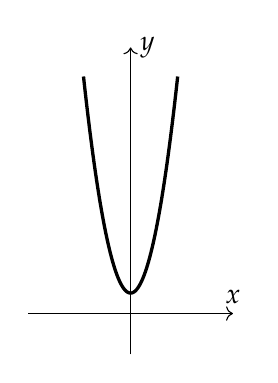
\begin{tikzpicture}[scale=0.26]
                    \draw[->] (-5,0) -- (5,0) node[above] {$x$};
                    \draw[->] (0,-2) -- (0,13) node[right] {$y$};
                    \draw[shift={(0,0)}] (0,0.1) -- (0,-0.1);
                    \draw[shift={(0,0)}] (0.1,0) -- (-0.1,0);
                    \draw[black,smooth,very thick,samples=100,domain=-2.3:2.3]
                        plot(\x,{2*\x*\x+1});
                \end{tikzpicture}
            }\qquad
            \subfigure[满足($a>0~~~~s<0$)]
            {
                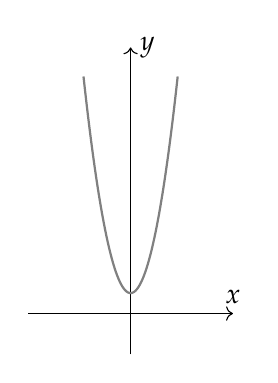
\begin{tikzpicture}[scale=0.26]
                    \draw[->] (-5,0) -- (5,0) node[above] {$x$};
                    \draw[->] (0,-2) -- (0,13) node[right] {$y$};
                    \draw[shift={(0,0)}] (0,0.1) -- (0,-0.1);
                    \draw[shift={(0,0)}] (0.1,0) -- (-0.1,0);
                    \draw[gray,smooth,thick,samples=100,domain=-2.3:2.3]
                        plot(\x,{2*\x*\x+1});
                \end{tikzpicture}
            }\qquad
            \subfigure[满足($a<0~~~~s>0$)]
            {
                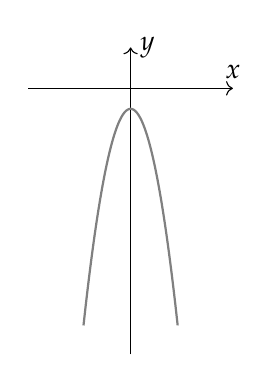
\begin{tikzpicture}[scale=0.26]
                    \draw[->] (-5,0) -- (5,0) node[above] {$x$};
                    \draw[->] (0,-13) -- (0,2) node[right] {$y$};
                    \draw[shift={(0,0)}] (0,0.1) -- (0,-0.1);
                    \draw[shift={(0,0)}] (0.1,0) -- (-0.1,0);
                    \draw[gray,smooth,thick,samples=100,domain=-2.3:2.3]
                        plot(\x,{-2*\x*\x-1});
                \end{tikzpicture}
            }\qquad
            \subfigure[满足($a<0~~~~s<0$)]
            {
                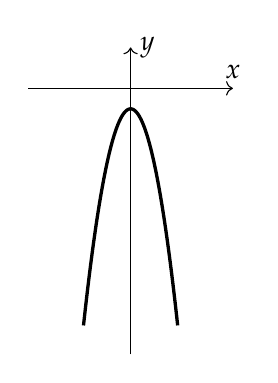
\begin{tikzpicture}[scale=0.26]
                    \draw[->] (-5,0) -- (5,0) node[above] {$x$};
                    \draw[->] (0,-13) -- (0,2) node[right] {$y$};
                    \draw[shift={(0,0)}] (0,0.1) -- (0,-0.1);
                    \draw[shift={(0,0)}] (0.1,0) -- (-0.1,0);
                    \draw[black,smooth,very thick,samples=100,domain=-2.3:2.3]
                        plot(\x,{-2*\x*\x-1});
                \end{tikzpicture}
            }
            \caption{满足$\Delta<0$时的图像}
        \end{center}
    \end{figure}\\
    当一元二次不等式满足$\Delta<0$时,性质总结如下:\vspace{5pt}
    \begin{table}[h]
        \begin{center}
            \begin{tabular}{l|l|l}
                \hline
                满足条件~~~~~~~~~~~~&符号不能取等~~~~~~~~~~~~~~~~~~~~&符号可以取等~~~~~~~~~~~~~~~~~~~~\\ \hline
                $a\cdot s>0$&$\mathbb{R}$&$\mathbb{R}$\\ \hline
                $a\cdot s<0$&$\emptyset$&$\emptyset$\\ \hline
            \end{tabular}
            \caption{满足$\Delta<0$时的性质总结}
        \end{center}
    \end{table}\\
    以上图像中,黑色部分代表在解集内,灰色部分代表在解集外。

\newpage

\subsubsection{一元二次不等式在$\Delta=0$时的情况}
    当一元二次不等式满足$\Delta=0$时,且符号不能取等时,图像如下:
    \begin{figure}[h!]
        \begin{center}
            \subfigure[满足($a>0~~~~s>0$)]
            {
                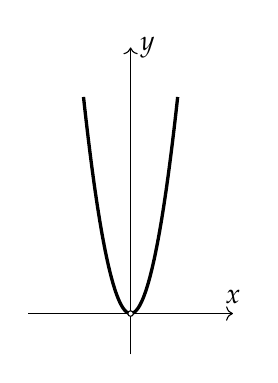
\begin{tikzpicture}[scale=0.26]
                    \draw[->] (-5,0) -- (5,0) node[above] {$x$};
                    \draw[->] (0,-2) -- (0,13) node[right] {$y$};
                    \draw[shift={(0,0)}] (0,0.1) -- (0,-0.1);
                    \draw[shift={(0,0)}] (0.1,0) -- (-0.1,0);
                    \draw[black,smooth,very thick,samples=100,domain=-2.3:2.3]
                        plot(\x,{2*\x*\x});
                    \tkzDefPoint(0,0){O}
                    \tkzDrawPoints[fill=white](O)
                \end{tikzpicture}
            }\qquad
            \subfigure[满足($a>0~~~~s<0$)]
            {
                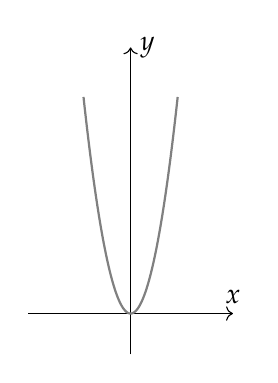
\begin{tikzpicture}[scale=0.26]
                    \draw[->] (-5,0) -- (5,0) node[above] {$x$};
                    \draw[->] (0,-2) -- (0,13) node[right] {$y$};
                    \draw[shift={(0,0)}] (0,0.1) -- (0,-0.1);
                    \draw[shift={(0,0)}] (0.1,0) -- (-0.1,0);
                    \draw[gray,smooth,thick,samples=100,domain=-2.3:2.3]
                        plot(\x,{2*\x*\x});
                \end{tikzpicture}
            }\qquad
            \subfigure[满足($a<0~~~~s>0$)]
            {
                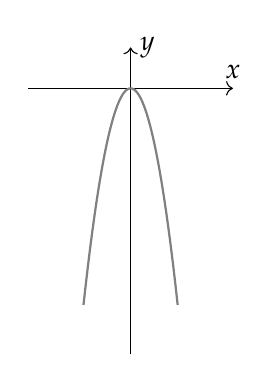
\begin{tikzpicture}[scale=0.26]
                    \draw[->] (-5,0) -- (5,0) node[above] {$x$};
                    \draw[->] (0,-13) -- (0,2) node[right] {$y$};
                    \draw[shift={(0,0)}] (0,0.1) -- (0,-0.1);
                    \draw[shift={(0,0)}] (0.1,0) -- (-0.1,0);
                    \draw[gray,smooth,thick,samples=100,domain=-2.3:2.3]
                        plot(\x,{-2*\x*\x});
                \end{tikzpicture}
            }\qquad
            \subfigure[满足($a<0~~~~s<0$)]
            {
                \begin{tikzpicture}[scale=0.26]
                    \draw[->] (-5,0) -- (5,0) node[above] {$x$};
                    \draw[->] (0,-13) -- (0,2) node[right] {$y$};
                    \draw[shift={(0,0)}] (0,0.1) -- (0,-0.1);
                    \draw[shift={(0,0)}] (0.1,0) -- (-0.1,0);
                    \draw[black,smooth,very thick,samples=100,domain=-2.3:2.3]
                        plot(\x,{-2*\x*\x});
                    \tkzDefPoint(0,0){O}
                    \tkzDrawPoints[fill=white](O)
                \end{tikzpicture}
            }
            \caption{满足$\Delta=0$时的图像(不能取等)}
        \end{center}
    \end{figure}\\
    当一元二次不等式满足$\Delta=0$时,且符号可以取等时,图像如下:
    \begin{figure}[h!]
        \begin{center}
            \subfigure[满足($a>0~~~~s>0$)]
            {
                \begin{tikzpicture}[scale=0.26]
                    \draw[->] (-5,0) -- (5,0) node[above] {$x$};
                    \draw[->] (0,-2) -- (0,13) node[right] {$y$};
                    \draw[shift={(0,0)}] (0,0.1) -- (0,-0.1);
                    \draw[shift={(0,0)}] (0.1,0) -- (-0.1,0);
                    \draw[black,smooth,very thick,samples=100,domain=-2.3:2.3]
                        plot(\x,{2*\x*\x});
                \end{tikzpicture}
            }\qquad
            \subfigure[满足($a>0~~~~s<0$)]
            {
                \begin{tikzpicture}[scale=0.26]
                    \draw[->] (-5,0) -- (5,0) node[above] {$x$};
                    \draw[->] (0,-2) -- (0,13) node[right] {$y$};
                    \draw[shift={(0,0)}] (0,0.1) -- (0,-0.1);
                    \draw[shift={(0,0)}] (0.1,0) -- (-0.1,0);
                    \draw[gray,smooth,thick,samples=100,domain=-2.3:2.3]
                        plot(\x,{2*\x*\x});
                    \tkzDefPoint(0,0){O}
                    \tkzDrawPoints[fill=black](O)
                \end{tikzpicture}
            }\qquad
            \subfigure[满足($a<0~~~~s>0$)]
            {
                \begin{tikzpicture}[scale=0.26]
                    \draw[->] (-5,0) -- (5,0) node[above] {$x$};
                    \draw[->] (0,-13) -- (0,2) node[right] {$y$};
                    \draw[shift={(0,0)}] (0,0.1) -- (0,-0.1);
                    \draw[shift={(0,0)}] (0.1,0) -- (-0.1,0);
                    \draw[gray,smooth,thick,samples=100,domain=-2.3:2.3]
                        plot(\x,{-2*\x*\x});
                    \tkzDefPoint(0,0){O}
                    \tkzDrawPoints[fill=black](O)
                \end{tikzpicture}
            }\qquad
            \subfigure[满足($a<0~~~~s<0$)]
            {
                \begin{tikzpicture}[scale=0.26]
                    \draw[->] (-5,0) -- (5,0) node[above] {$x$};
                    \draw[->] (0,-13) -- (0,2) node[right] {$y$};
                    \draw[shift={(0,0)}] (0,0.1) -- (0,-0.1);
                    \draw[shift={(0,0)}] (0.1,0) -- (-0.1,0);
                    \draw[black,smooth,very thick,samples=100,domain=-2.3:2.3]
                        plot(\x,{-2*\x*\x});
                \end{tikzpicture}
            }
            \caption{满足$\Delta=0$时的图像(可以取等)}
        \end{center}
    \end{figure}\\
    当一元二次不等式满足$\Delta=0$时,性质总结如下:\vspace{5pt}
    \begin{table}[h!]
        \begin{center}
            \begin{tabular}{l|l|l}
                \hline
                满足条件~~~~~~~~~~~~&符号不取等~~~~~~~~~~~~~~~~~~~~&符号取等~~~~~~~~~~~~~~~~~~~~\\ \hline
                $a\cdot s>0$&$x\neq x_0$&$\mathbb{R}$\\ \hline
                $a\cdot s<0$&$\emptyset$&$x=x_0$\\ \hline
            \end{tabular}
            \caption{满足$\Delta=0$时的性质总结}
        \end{center}
    \end{table}\\
    以上图像中,黑色部分代表在解集内,灰色部分代表在解集外。\\[3mm]
    当满足$a\cdot s>0$时,即当二次项系数和符号同号时,整根曲线都取,不能取等时需挖去顶点。\\[3mm]
    当满足$a\cdot s<0$时,即当二次项系数和符号异号时,整根曲线不取,可以取等时仅包含顶点。

\newpage

\subsubsection{一元二次不等式在$\Delta>0$时的情况}
    当一元二次不等式满足$\Delta>0$时,且符号不能取等时,图像如下:
    \begin{figure}[h!]
        \begin{center}
            \subfigure[满足($a>0~~~~s>0$)]
            {
                \begin{tikzpicture}[scale=0.26]
                    \draw[->] (-5,0) -- (5,0) node[above] {$x$};
                    \draw[->] (0,-2) -- (0,13) node[right] {$y$};
                    \draw[shift={(0,0)}] (0,0.1) -- (0,-0.1);
                    \draw[shift={(0,0)}] (0.1,0) -- (-0.1,0);
                    \draw[black,smooth,very thick,samples=100,domain=-2.3:-0.721]
                        plot(\x,{2*\x*\x-1});
                    \draw[black,smooth,very thick,samples=100,domain=+0.721:+2.3]
                        plot(\x,{2*\x*\x-1});
                    \draw[gray,smooth,thick,samples=100,domain=-0.721:+0.721]
                        plot(\x,{2*\x*\x-1});
                    \tkzDefPoint(-0.721,0){A}
                    \tkzDefPoint(+0.721,0){B}
                    \tkzDrawPoints[fill=white](A,B)
                \end{tikzpicture}
            }\qquad
            \subfigure[满足($a>0~~~~s<0$)]
            {
                \begin{tikzpicture}[scale=0.26]
                    \draw[->] (-5,0) -- (5,0) node[above] {$x$};
                    \draw[->] (0,-2) -- (0,13) node[right] {$y$};
                    \draw[shift={(0,0)}] (0,0.1) -- (0,-0.1);
                    \draw[shift={(0,0)}] (0.1,0) -- (-0.1,0);
                    \draw[gray,smooth,thick,samples=100,domain=-2.3:-0.721]
                        plot(\x,{2*\x*\x-1});
                    \draw[gray,smooth,thick,samples=100,domain=+0.721:+2.3]
                        plot(\x,{2*\x*\x-1});
                    \draw[black,smooth,very thick,samples=100,domain=-0.721:+0.721]
                        plot(\x,{2*\x*\x-1});
                    \tkzDefPoint(-0.721,0){A}
                    \tkzDefPoint(+0.721,0){B}
                    \tkzDrawPoints[fill=white](A,B)
                \end{tikzpicture}
            }\qquad
            \subfigure[满足($a<0~~~~s>0$)]
            {
                \begin{tikzpicture}[scale=0.26]
                    \draw[->] (-5,0) -- (5,0) node[above] {$x$};
                    \draw[->] (0,-13) -- (0,2) node[right] {$y$};
                    \draw[shift={(0,0)}] (0,0.1) -- (0,-0.1);
                    \draw[shift={(0,0)}] (0.1,0) -- (-0.1,0);
                    \draw[gray,smooth,thick,samples=100,domain=-2.3:-0.721]
                        plot(\x,{-2*\x*\x+1});
                    \draw[gray,smooth,thick,samples=100,domain=+0.721:+2.3]
                        plot(\x,{-2*\x*\x+1});
                    \draw[black,smooth,very thick,samples=100,domain=-0.721:+0.721]
                        plot(\x,{-2*\x*\x+1});
                    \tkzDefPoint(-0.721,0){A}
                    \tkzDefPoint(+0.721,0){B}
                    \tkzDrawPoints[fill=white](A,B)
                \end{tikzpicture}
            }\qquad
            \subfigure[满足($a<0~~~~s<0$)]
            {
                \begin{tikzpicture}[scale=0.26]
                    \draw[->] (-5,0) -- (5,0) node[above] {$x$};
                    \draw[->] (0,-13) -- (0,2) node[right] {$y$};
                    \draw[shift={(0,0)}] (0,0.1) -- (0,-0.1);
                    \draw[shift={(0,0)}] (0.1,0) -- (-0.1,0);
                    \draw[black,smooth,very thick,samples=100,domain=-2.3:-0.721]
                        plot(\x,{-2*\x*\x+1});
                    \draw[black,smooth,very thick,samples=100,domain=+0.721:+2.3]
                        plot(\x,{-2*\x*\x+1});
                    \draw[gray,smooth,thick,samples=100,domain=-0.721:+0.721]
                        plot(\x,{-2*\x*\x+1});
                    \tkzDefPoint(-0.721,0){A}
                    \tkzDefPoint(+0.721,0){B}
                    \tkzDrawPoints[fill=white](A,B)
                \end{tikzpicture}
            }
            \caption{满足$\Delta>0$时的图像(不能取等)}
        \end{center}
    \end{figure}\\
    当一元二次不等式满足$\Delta>0$时,且符号可以取等时,图像如下:
    \begin{figure}[h!]
        \begin{center}
            \subfigure[满足($a>0~~~~s>0$)]
            {
                \begin{tikzpicture}[scale=0.26]
                    \draw[->] (-5,0) -- (5,0) node[above] {$x$};
                    \draw[->] (0,-2) -- (0,13) node[right] {$y$};
                    \draw[shift={(0,0)}] (0,0.1) -- (0,-0.1);
                    \draw[shift={(0,0)}] (0.1,0) -- (-0.1,0);
                    \draw[black,smooth,very thick,samples=100,domain=-2.3:-0.721]
                        plot(\x,{2*\x*\x-1});
                    \draw[black,smooth,very thick,samples=100,domain=+0.721:+2.3]
                        plot(\x,{2*\x*\x-1});
                    \draw[gray,smooth,thick,samples=100,domain=-0.721:+0.721]
                        plot(\x,{2*\x*\x-1});
                    \tkzDefPoint(-0.721,0){A}
                    \tkzDefPoint(+0.721,0){B}
                    \tkzDrawPoints[fill=black](A,B)
                \end{tikzpicture}
            }\qquad
            \subfigure[满足($a>0~~~~s<0$)]
            {
                \begin{tikzpicture}[scale=0.26]
                    \draw[->] (-5,0) -- (5,0) node[above] {$x$};
                    \draw[->] (0,-2) -- (0,13) node[right] {$y$};
                    \draw[shift={(0,0)}] (0,0.1) -- (0,-0.1);
                    \draw[shift={(0,0)}] (0.1,0) -- (-0.1,0);
                    \draw[gray,smooth,thick,samples=100,domain=-2.3:-0.721]
                        plot(\x,{2*\x*\x-1});
                    \draw[gray,smooth,thick,samples=100,domain=+0.721:+2.3]
                        plot(\x,{2*\x*\x-1});
                    \draw[black,smooth,very thick,samples=100,domain=-0.721:+0.721]
                        plot(\x,{2*\x*\x-1});
                    \tkzDefPoint(-0.721,0){A}
                    \tkzDefPoint(+0.721,0){B}
                    \tkzDrawPoints[fill=black](A,B)
                \end{tikzpicture}
            }\qquad
            \subfigure[满足($a<0~~~~s>0$)]
            {
                \begin{tikzpicture}[scale=0.26]
                    \draw[->] (-5,0) -- (5,0) node[above] {$x$};
                    \draw[->] (0,-13) -- (0,2) node[right] {$y$};
                    \draw[shift={(0,0)}] (0,0.1) -- (0,-0.1);
                    \draw[shift={(0,0)}] (0.1,0) -- (-0.1,0);
                    \draw[gray,smooth,thick,samples=100,domain=-2.3:-0.721]
                        plot(\x,{-2*\x*\x+1});
                    \draw[gray,smooth,thick,samples=100,domain=+0.721:+2.3]
                        plot(\x,{-2*\x*\x+1});
                    \draw[black,smooth,very thick,samples=100,domain=-0.721:+0.721]
                        plot(\x,{-2*\x*\x+1});
                    \tkzDefPoint(-0.721,0){A}
                    \tkzDefPoint(+0.721,0){B}
                    \tkzDrawPoints[fill=black](A,B)
                \end{tikzpicture}
            }\qquad
            \subfigure[满足($a<0~~~~s<0$)]
            {
                \begin{tikzpicture}[scale=0.26]
                    \draw[->] (-5,0) -- (5,0) node[above] {$x$};
                    \draw[->] (0,-13) -- (0,2) node[right] {$y$};
                    \draw[shift={(0,0)}] (0,0.1) -- (0,-0.1);
                    \draw[shift={(0,0)}] (0.1,0) -- (-0.1,0);
                    \draw[black,smooth,very thick,samples=100,domain=-2.3:-0.721]
                        plot(\x,{-2*\x*\x+1});
                    \draw[black,smooth,very thick,samples=100,domain=+0.721:+2.3]
                        plot(\x,{-2*\x*\x+1});
                    \draw[gray,smooth,thick,samples=100,domain=-0.721:+0.721]
                        plot(\x,{-2*\x*\x+1});
                    \tkzDefPoint(-0.721,0){A}
                    \tkzDefPoint(+0.721,0){B}
                    \tkzDrawPoints[fill=black](A,B)
                \end{tikzpicture}
            }
            \caption{满足$\Delta>0$时的图像(可以取等)}
        \end{center}
    \end{figure}\\
    当一元二次不等式满足$\Delta>0$时,性质总结如下:\vspace{5pt}
    \begin{table}[h!]
        \begin{center}
            \begin{tabular}{l|l|l}
                \hline
                满足条件~~~~~~~~~~~~&符号不取等~~~~~~~~~~~~~~~~~~~~&符号取等~~~~~~~~~~~~~~~~~~~~\\ \hline
                $a\cdot s>0$&$x<x_1~~$或$~~x>x_2$&$x\leq x_1~~$或$~~x\geq x_2$\\ \hline
                $a\cdot s<0$&$x>x_1~~$且$~~x<x_2$&$x\geq x_1~~$且$~~x\leq x_2$\\ \hline
            \end{tabular}
            \caption{满足$\Delta>0$时的性质总结}
        \end{center}
    \end{table}\\
    以上图像中,黑色部分代表在解集内,灰色部分代表在解集外。\\[3mm]
    当满足$a\cdot s>0$时,即当二次项系数和符号同号时,不等式的解集取两根之外。\\[3mm]
    当满足$a\cdot s<0$时,即当二次项系数和符号异号时,不等式的解集取两根之间。
    
\newpage

\subsection{根的分布}
    根的分布研究这样一类问题,给定方程的根的范围,求解一元二次方程参数需满足的条件。\\[3mm]
    根的分布的问题最终都可以通过分类讨论,化归为以下三类基本情况。

\subsubsection{根的分布的基本情况$1$}
    根的分布的基本情况$1$的条件如下:
    \begin{large}
        \begin{equation*}
            x_1\in(A,B)~~~~~~~~x_2\notin(A,B)~~~~~~~~(A<B)
        \end{equation*}
    \end{large}\\
    根的分布的基本情况$1$的示意图($a>0$):\vspace{3pt}
    \begin{figure}[h]
        \begin{center}
            \begin{tikzpicture}[scale=1.0]
                \draw[->] (-6,0) -- (6,0) node[above] {$x$};
                \draw[black,smooth,thick,samples=100,domain=-1.5:+4.5]
                    plot(\x,{+0.25*(\x-1.5)*(\x-1.5)-1});
                \draw[black,smooth,thick,samples=100,domain=-4.5:+1.5]
                    plot(\x,{+0.25*(\x+1.5)*(\x+1.5)-1});

                \draw (-2.5,0)--(-2.5,0.2);
                \draw (+2.5,0)--(+2.5,0.2);

                \node at(-2.5,-0.2) {$A$};
                \node at(+2.5,-0.2) {$B$};
            \end{tikzpicture}
            \caption{根的分布的基本情况$1$的示意图($a>0$)}
        \end{center}
    \end{figure}\\
    根的分布的基本情况$1$的示意图($a<0$):\vspace{3pt}
    \begin{figure}[h]
        \begin{center}
            \begin{tikzpicture}[scale=1.0]
                \draw[->] (-6,0) -- (6,0) node[above] {$x$};
                \draw[black,smooth,thick,samples=100,domain=-1.5:+4.5]
                    plot(\x,{-0.25*(\x-1.5)*(\x-1.5)+1});
                \draw[black,smooth,thick,samples=100,domain=-4.5:+1.5]
                    plot(\x,{-0.25*(\x+1.5)*(\x+1.5)+1});

                \draw (-2.5,0)--(-2.5,0.2);
                \draw (+2.5,0)--(+2.5,0.2);

                \node at(-2.5,-0.2) {$A$};
                \node at(+2.5,-0.2) {$B$};
            \end{tikzpicture}
            \caption{根的分布的基本情况$1$的示意图($a<0$)}
        \end{center}
    \end{figure}\\
    根的分布基本情况$1$的参数情况如下:\vspace{3pt}
    \begin{large}
        \begin{equation*}
            F(A)\cdot F(B)<0
        \end{equation*}
    \end{large}\\
    该式对于$a>0$和$a<0$的情况均是成立的。\\[3mm]
    在该情况中,我们认为有$x_1\neq x_2$,故无需讨论$x_1=x_2$,即$\Delta=0$时的情况。\\[3mm]
    在该情况中,如果条件中任意一侧的开区间变为闭区间,则参数情况中的小于需改为小于等于。

\newpage

\subsubsection{根的分布基本情况$2$}
    根的分布基本情况$2$的条件如下:
    \begin{large}
        \begin{equation*}
            x_1\in(A,B)~~~~~~~~x_2\in(A,B)~~~~~~~~(A<B)
        \end{equation*}
    \end{large}\\
    根的分布基本情况$2$的示意图($a>0$):\vspace{5pt}
    \begin{figure}[h]
        \begin{center}
            \begin{tikzpicture}
                \draw[->] (-6,0) -- (6,0) node[above] {$x$};
                \draw[black,smooth,thick,samples=100,domain=-3:+3]
                    plot(\x,{+0.25*\x*\x-1});

                \draw (-2.5,0)--(-2.5,0.2);
                \draw (+2.5,0)--(+2.5,0.2);

                \node at(-2.5,-0.2) {$A$};
                \node at(+2.5,-0.2) {$B$};
            \end{tikzpicture}
            \caption{根的分布基本情况$2$的示意图($a>0$)}
        \end{center}
    \end{figure}\\
    根的分布基本情况$2$的示意图($a<0$):\vspace{5pt}
    \begin{figure}[h]
        \begin{center}
            \begin{tikzpicture}
                \draw[->] (-6,0) -- (6,0) node[above] {$x$};
                \draw[black,smooth,thick,samples=100,domain=-3:+3]
                    plot(\x,{-0.25*\x*\x+1});

                \draw (-2.5,0)--(-2.5,0.2);
                \draw (+2.5,0)--(+2.5,0.2);

                \node at(-2.5,-0.2) {$A$};
                \node at(+2.5,-0.2) {$B$};
            \end{tikzpicture}
            \caption{根的分布基本情况$2$的示意图($a<0$)}
        \end{center}
    \end{figure}\\
    根的分布基本情况$2$的参数情况如下:\vspace{5pt}
    \begin{large}
        \begin{equation*}
            \begin{cases}
                ~~F(A)>0\\[4mm]
                ~~F(B)>0\\[4mm]
                ~~-\dfrac{b}{2a}>A\\[4mm]
                ~~-\dfrac{b}{2a}<B\\[4mm]
                ~~\Delta>0\\[1mm]
            \end{cases}
            ~~(a>0)
            ~~~~~~~~~~~~~~~~
            \begin{cases}
                ~~F(A)<0\\[4mm]
                ~~F(B)<0\\[4mm]
                ~~-\dfrac{b}{2a}>A\\[4mm]
                ~~-\dfrac{b}{2a}<B\\[4mm]
                ~~\Delta>0\\[1mm]
            \end{cases}
            ~~(a<0)
        \end{equation*}
    \end{large}\\[1mm]
    在该情况中,允许$A=-\infty$,允许$B=+\infty$,包含无穷的条件视为无效。\\[3mm]
    在该情况中,若条件中某个字母一侧由开区间变为闭区间,则参数情况中含该字母的符号取等。

\newpage

\subsubsection{根的分布基本情况$3$}
    根的分布基本情况$3$的条件如下:
    \begin{large}
        \begin{equation*}
            x_1\in(A,B)~~~~~~~~x_2\in(C,D)~~~~~~~~(A<B\leq C<D)
        \end{equation*}
    \end{large}\\
    根的分布基本情况$3$的示意图如下($a>0$):\vspace{5pt}
    \begin{figure}[h]
        \begin{center}
            \begin{tikzpicture}
                \draw[->] (-6,0) -- (6,0) node[above] {$x$};
                \draw[black,smooth,thick,samples=100,domain=-3:+3]
                    plot(\x,{+0.25*\x*\x-1});

                \draw (-2.5,0)--(-2.5,0.2);
                \draw (-1.5,0)--(-1.5,0.2);
                \draw (+1.5,0)--(+1.5,0.2);
                \draw (+2.5,0)--(+2.5,0.2);

                \node at(-2.5,-0.2) {$A$};
                \node at(-1.5,-0.2) {$B$};
                \node at(+1.5,-0.2) {$C$};
                \node at(+2.5,-0.2) {$D$};
            \end{tikzpicture}
            \caption{根的分布基本情况$3$的示意图($a>0$)}
        \end{center}
    \end{figure}\\
    根的分布基本情况$3$的示意图如下($a<0$):\vspace{5pt}
    \begin{figure}[h]
        \begin{center}
            \begin{tikzpicture}
                \draw[->] (-6,0) -- (6,0) node[above] {$x$};
                \draw[black,smooth,thick,samples=100,domain=-3:+3]
                    plot(\x,{-0.25*\x*\x+1});

                \draw (-2.5,0)--(-2.5,0.2);
                \draw (-1.5,0)--(-1.5,0.2);
                \draw (+1.5,0)--(+1.5,0.2);
                \draw (+2.5,0)--(+2.5,0.2);

                \node at(-2.5,-0.2) {$A$};
                \node at(-1.5,-0.2) {$B$};
                \node at(+1.5,-0.2) {$C$};
                \node at(+2.5,-0.2) {$D$};
            \end{tikzpicture}
            \caption{根的分布基本情况$3$的示意图($a<0$)}
        \end{center}
    \end{figure}\\
    根的分布基本情况$3$的参数如下:\vspace{8pt}
    \begin{large}
        \begin{equation*}
            \begin{cases}
                ~~F(A)>0\\[6mm]
                ~~F(B)<0\\[6mm]
                ~~F(C)<0\\[6mm]
                ~~F(D)>0\\[1mm]
            \end{cases}
            ~~(a>0)
            ~~~~~~~~~~~~~~~~
            \begin{cases}
                ~~F(A)<0\\[6mm]
                ~~F(B)>0\\[6mm]
                ~~F(C)>0\\[6mm]
                ~~F(D)<0\\[1mm]
            \end{cases}
            ~~(a<0)
        \end{equation*}
    \end{large}\\[1mm]
    在这一情况中,允许$A=-\infty$,允许$D=+\infty$,包含无穷的条件视为无效。\\[3mm]
    在该情况中,若条件中某个字母一侧由开区间变为闭区间,则参数情况中含该字母的符号取等。

\newpage

\subsection{分式不等式的求解}
    \setcounter{equation}{0}
    分式不等式的求解需要利用以下同解原理。\\[3mm]
    分式不等式的同解原理$1$:
    \begin{large}
        \begin{equation*}
            \frac{f(x)}{g(x)}>0~~~~\Longleftrightarrow~~~~f(x)\cdot g(x)>0
        \end{equation*}
    \end{large}\\
    分式不等式的同解原理$2$:
    \begin{large}
        \begin{equation*}
            \frac{f(x)}{g(x)}<0~~~~\Longleftrightarrow~~~~f(x)\cdot g(x)<0
        \end{equation*}
    \end{large}\\
    由于$\dfrac{f(x)}{g(x)}>0$和$f(x)\cdot g(x)>0$均只有在$f(x)$和$g(x)$同号时成立,因此同解原理$1$成立。\\[5mm]
    由于$\dfrac{f(x)}{g(x)}<0$和$f(x)\cdot g(x)<0$均只有在$f(x)$和$g(x)$异号时成立,因此同解原理$2$成立。\\[7mm]
    求解分式不等式需注意下式并不成立:\vspace{3pt}
    \begin{align}           
        &~~~~\frac{f(x)}{g(x)}>a~~~~\Longleftrightarrow~~~~f(x)\cdot g(x)>a~~~~~~~~\text{\small(错误!)}\\[4mm]
        &~~~~\frac{f(x)}{g(x)}<a~~~~\Longleftrightarrow~~~~f(x)\cdot g(x)<a~~~~~~~~\text{\small(错误!)}
    \end{align}\\
    如果分式不等式右侧的数不为零,不能直接套用同解原理公式,应当先移至左侧通分。\\[8mm]
    分式不等式的同解原理$3$:
    \begin{large}
        \begin{equation*}
            \frac{f(x)}{g(x)}\geq 0~~~~\Longleftrightarrow~~~~
            \begin{cases}
                ~f(x)\cdot g(x)\geq 0\\[1mm]
                ~g(x)\neq 0\\
            \end{cases}
        \end{equation*}
    \end{large}\\
    分式不等式的同解原理$4$:
    \begin{large}
        \begin{equation*}
            \frac{f(x)}{g(x)}\leq 0~~~~\Longleftrightarrow~~~~
            \begin{cases}
                ~f(x)\cdot g(x)\leq 0\\[1mm]
                ~g(x)\neq 0\\
            \end{cases}
        \end{equation*}
    \end{large}\\
    此处右侧的$f(x)\cdot g(x)$可以在$f(x)=0$或$g(x)=0$时成立。\\[5mm]
    然而左侧的$\dfrac{f(x)}{g(x)}$中由于作为分母$g(x)$不能为零,因此右侧需添加$g(x)\neq 0$的条件。

\newpage

\subsection{无理不等式的求解}
    无理不等式的求解需要利用以下同解原理。\\[3mm]
    无理不等式的同解原理$1$:
    \begin{large}
        \begin{equation*}
            \sqrt{f(x)}<\sqrt{g(x)}~~~~\Longleftrightarrow~~~~
            \begin{cases}
                ~f(x)\geq 0\\[1mm]
                ~g(x)\geq 0\\[1mm]
                ~f(x)<g(x)\\[1mm]
            \end{cases}
        \end{equation*}
    \end{large}\\
    无理不等式的同解原理$2$:
    \begin{large}
        \begin{equation*}
            \sqrt{f(x)}>\sqrt{g(x)}~~~~\Longleftrightarrow~~~~
            \begin{cases}
                ~f(x)\geq 0\\[1mm]
                ~g(x)\geq 0\\[1mm]
                ~f(x)>g(x)\\[1mm]
            \end{cases}
        \end{equation*}
    \end{large}\\
    由于$\sqrt{f(x)}$中$f(x)$处在根号下,因此需满足$f(x)\geq 0$。\\[3mm]
    由于$\sqrt{g(x)}$中$g(x)$处在根号下,因此需满足$g(x)\geq 0$。\\[3mm]
    根据不等式的乘方性质可以由$\sqrt{f(x)}<\sqrt{g(x)}$推出$f(x)<g(x)$,因此同解原理$1$成立。\\[3mm]
    根据不等式的乘方性质可以由$\sqrt{f(x)}>\sqrt{g(x)}$推出$f(x)>g(x)$,因此同解原理$2$成立。\\[6mm]
    无理不等式的同解原理$3$:
    \begin{large}
        \begin{equation*}
            \sqrt{f(x)}<g(x)~~~~\Longleftrightarrow~~~~
            \begin{cases}
                ~f(x)\geq 0\\[1mm]
                ~g(x)> 0\\[1mm]
                ~f(x)<g^2(x)\\[1mm]
            \end{cases}~~~~~~~~~~~~~~~~~~~~\;
        \end{equation*}
    \end{large}\\
    无理不等式的同解原理$4$:
    \begin{large}
        \begin{equation*}
            ~~~~~~~~~~~~~~~~
            \sqrt{f(x)}>g(x)~~~~\Longleftrightarrow~~~~
            \begin{cases}
                ~f(x)\geq 0\\[1mm]
                ~g(x)\geq 0\\[1mm]
                ~f(x)>g^2(x)\\[1mm]
            \end{cases}
            \text{或}~~~~~~~~
            \begin{cases}
                ~f(x)\geq 0\\[1mm]
                ~g(x)<0\\[1mm]
            \end{cases}
        \end{equation*}
    \end{large}\\
    其中在无理不等式的同解原理$4$中由于$\sqrt{f(x)}\geq 0$,因此当$g(x)<0$时不等式恒成立。

\newpage

\subsection{绝对值不等式的求解}
    绝对值不等式的求解需要利用以下同解原理。\\[3mm]
    绝对值不等式的同解原理$1$:
    \begin{large}
        \begin{equation*}
            \big|f(x)\big|<a~~(a>0)~~~~\Longleftrightarrow~~~~\big\{x~|~x>-a~~\text{且}~~x<a\big\}
        \end{equation*}
    \end{large}\\
    绝对值不等式的同解原理$2$:
    \begin{large}
        \begin{equation*}
            \big|f(x)\big|>a~~(a>0)~~~~\Longleftrightarrow~~~~\big\{x~|~x<-a~~\text{或}~~x>a\big\}
        \end{equation*}
    \end{large}\\
    绝对值不等式的同解原理$1$可以由其图像证明:
    \begin{figure}[h]
        \begin{center}
            \begin{tikzpicture}
                \tkzDefPoint(0,0){O}
                \tkzDefPoint(-5,0){X1}
                \tkzDefPoint(+5,0){X2}
                \tkzDrawSegment[->](X1,X2)
                \tkzLabelPoint[above](X2){$x$}

                \tkzDefPoint(-2,0){A}
                \tkzDefPoint(+2,0){B}

                \tkzDefShiftPoint[A](0,0.5){A1}
                \tkzDefShiftPoint[B](0,0.5){B1}

                \tkzDrawSegments(A,A1 B,B1 A1,B1)
                \tkzDrawPoints[fill=white](A,B)

                \tkzLabelPoint[below](A){$-a$}
                \tkzLabelPoint[below](B){$+a$}
                
                \tkzLabelPoint[below](O){$0$}
                \tkzLabelPoint[above=20pt](O){$|x|<a$}
            \end{tikzpicture}
            \caption{绝对值不等式的同解原理$1$}
        \end{center}
    \end{figure}\\
    绝对值不等式的同解原理$2$可以由其图像证明:
    \begin{figure}[h]
        \begin{center}
            \begin{tikzpicture}
                \tkzDefPoint(0,0){O}
                \tkzDefPoint(-5,0){X1}
                \tkzDefPoint(+5,0){X2}
                \tkzDrawSegment[->](X1,X2)
                \tkzLabelPoint[above](X2){$x$}

                \tkzDefPoint(-2,0){A}
                \tkzDefPoint(+2,0){B}

                \tkzDefShiftPoint[A](0,0.5){A1}
                \tkzDefShiftPoint[B](0,0.5){B1}

                \tkzDefShiftPoint[A1](-2,0){A2}
                \tkzDefShiftPoint[B1](+2,0){B2}

                \tkzDrawSegments(A,A1 B,B1 A1,A2 B1,B2)
                \tkzDrawPoints[fill=white](A,B)

                \tkzLabelPoint[below](A){$-a$}
                \tkzLabelPoint[below](B){$+a$}
                
                \tkzLabelPoint[below](O){$0$}
                \tkzLabelPoint[above=20pt](O){$|x|>a$}
            \end{tikzpicture}
            \caption{绝对值不等式的同解原理$2$}
        \end{center}
    \end{figure}\\
    绝对值不等式的同解原理$3$:
    \begin{large}
        \begin{equation*}
            \big|f(x)\big|<\big|g(x)\big|~~~~\Rightarrow~~~~f^2(x)<g^2(x)
        \end{equation*}
    \end{large}\\
    绝对值不等式的同解原理$4$:
    \begin{large}
        \begin{equation*}
            \big|f(x)\big|>\big|g(x)\big|~~~~\Rightarrow~~~~f^2(x)>g^2(x)
        \end{equation*}
    \end{large}\\
    绝对值不等式的同解原理的$3$和$4$可以由不等式的乘方法则证明。

\newpage

\subsection{基本不等式$1$}
    基本不等式$1$的基本形式:
    \begin{large}
        \begin{equation*}
            a^2+b^2 \geq 2\cdot a\cdot b~~~~~~~~a,b\in\mathbb{R}~~~~~~~~\text{(当且仅当$a=b$时等号成立)}
        \end{equation*}
    \end{large}\\
    基本不等式$1$的扩展形式:\vspace{3pt}
    \begin{large}
        \begin{equation*}
            ~~~~
            \begin{cases}
                ~2\cdot a\cdot b\leq+(a^2+b^2) ~~~~~~~~a,b\in\mathbb{R}~~~~~~~~\text{(当且仅当$a=+b$时等号成立)}\\[1mm]
                ~2\cdot a\cdot b\geq-(a^2+b^2)~~~~~~~~a,b\in\mathbb{R}~~~~~~~~\text{(当且仅当$a=-b$时等号成立)}\\[1mm]
            \end{cases}
        \end{equation*}
    \end{large}\\[5mm]
    当满足$a=+b$时有:
    \setcounter{equation}{0}
    \begin{align}
        2\cdot a\cdot b=+(a^2+b^2)
    \end{align}\\
    当满足$a\neq +b$时有:
    \begin{align}
        &(a-b)^2>0\\[2mm]
        &~a^2-2\cdot a\cdot b+b^2>0\\[2mm]
        &~a^2+b^2>2\cdot a\cdot b\\[2mm]
        &~2\cdot a\cdot b<+(a^2+b^2)
    \end{align}\\
    当满足$a=-b$时有:
    \begin{align}
        2\cdot a\cdot b=-(a^2+b^2)
    \end{align}\\
    当满足$a\neq -b$时有:
    \begin{align}
        &(a+b)^2>0\\[2mm]
        &~a^2+2\cdot a\cdot b+b^2>0\\[2mm]
        &~a^2+b^2>-2\cdot a\cdot b\\[2mm]
        &~2\cdot a\cdot b>-(a^2+b^2)
    \end{align}\\
    由此证明了基本不等式$1$的基本形式和扩展形式成立。

\newpage

\subsection{基本不等式$2$}
    基本不等式$2$的基本形式:
    \begin{large}
        \begin{equation*}
            a+b \geq 2\cdot\sqrt{a\cdot b}~~~~~~~a,b\in\mathbb{R^+}~~~~~~\text{(当且仅当$a=b$时等号成立)}
        \end{equation*}
    \end{large}\\
    基本不等式$2$的扩展形式:\vspace{3pt}
    \begin{large}
        \begin{equation*}
            ~~~~
            \begin{cases}
                ~a+b\geq +2\cdot\sqrt{a\cdot b}~~~~~~~~~~a,b\in\mathbb{R^+}~~~~~~~~\text{(当且仅当$a=b$时等号成立)}\\[1mm]
                ~a+b\leq -2\cdot\sqrt{a\cdot b}~~~~~~~~~~a,b\in\mathbb{R^-}~~~~~~~~\text{(当且仅当$a=b$时等号成立)}\\[1mm]
            \end{cases}
        \end{equation*}
    \end{large}\\[2mm]
    当满足$a^{'}>0$且$b^{'}>0$时可以进行以下代换:
    \setcounter{equation}{0}
    \begin{align}
        &a=\sqrt{a^{'}}~~~~~~b=\sqrt{b^{'}}\\[2mm]
        &a^2=a^{'}~~~~~~b^2=b^{'}
    \end{align}\\
    代入基本不等式$1$的基本形式可得:
    \begin{align}
        &a^2+b^2\geq 2\cdot a\cdot b\\[3mm]
        &a^{'}+b^{'}\geq 2\cdot\sqrt{a^{'}}\cdot\sqrt{b^{'}}\\[3mm]
        &a^{'}+b^{'}\geq 2\cdot\sqrt{a^{'}\cdot b^{'}}\\[3mm]
        &a^{'}+b^{'}\geq +2\cdot\sqrt{a^{'}\cdot b^{'}}
    \end{align}\\
    当满足$a^{'}<0$且$b^{'}<0$时可以进行以下代换:
    \begin{align}
        &a=-\sqrt{-a^{'}}~~~~~~b=-\sqrt{-b^{'}}\\[2mm]
        &a^2=-a^{'}~~~~~~b^2=-b^{'}
    \end{align}\\
    代入基本不等式$1$的基本形式可得:
    \begin{align}
        &a^2+b^2\geq 2\cdot a\cdot b\\[3mm]
        &-a^{'}-b^{'}\geq 2\cdot\sqrt{-a^{'}}\cdot\sqrt{-b^{'}}\\[3mm]
        &-a^{'}-b^{'}\geq 2\cdot\sqrt{a^{'}\cdot b^{'}}\\[3mm]
        &a^{'}+b^{'}\leq -2\cdot\sqrt{a^{'}\cdot b^{'}}
    \end{align}\\
    由此证明了基本不等式$2$的基本形式和扩展形式成立。

\newpage

\subsubsection{使用基本不等式求解函数最值$1$}
    求解形如下方的函数的最值:
    \setcounter{equation}{0}
    \begin{equation}
        f(x)=\frac{a\cdot x^2+b\cdot x+c}{d\cdot x+e}
    \end{equation}\\
    定义代换变量$t$代换$x$有:
    \begin{align}
        t=d\cdot x+e
    \end{align}\\
    用变量$t$将$x$反表示则有:
    \begin{align}
        x=\frac{1}{d}\cdot(t-e)
    \end{align}\\
    即变量$x$可以表示为关于代换变量$t$的函数,记之为函数$x=g(t)$。\\[16mm]
    将其代入函数$f(x)$可得:
    \begin{align}
        &f(x)=\frac{a\cdot x^2+b\cdot x+c}{d\cdot x+e}\\[3mm]
        &f(t)=\frac{a\cdot g(t)^2+b\cdot g(t)+c}{t}\\[3mm]
        &f(t)=\frac{A\cdot t^2+B\cdot t+C}{t}\\[3mm]
        &f(t)=A\cdot t+B+C\cdot\frac{1}{t}\\[3mm]
        &f(t)=A\cdot t+C\cdot\frac{1}{t}+B
    \end{align}\\
    观察函数$f(t)$可以发现:
    \begin{align}
        f(t)=\underbrace{\left(A\cdot t+C\cdot\frac{1}{t}\right)}_{\text{基本不等式2}}+B
    \end{align}\\
    因此此时即可通过基本不等式$2$求解函数最值。

\newpage

    上述第五步至第六步的推导如下:
    \begin{align}
        &f(t)=\frac{1}{t}\cdot\left[a\cdot g(t)^2+b\cdot g(t)+c\right]\\[4mm]
        &f(t)=\frac{1}{t}\cdot\left[\frac{a}{d^2}\cdot(t-e)^2+\frac{b}{d}\cdot(t-e)+c\right]\\[4mm]
        &f(t)=\frac{1}{t}\cdot\left[t^2\cdot\frac{a}{d^2}-t\cdot\frac{2ae}{d^2}+\frac{ae^2}{d^2}+t\cdot\frac{b}{d}-\frac{be}{d}+c\right]\\[4mm]
        &f(t)=\frac{1}{t}\cdot\left[t^2\cdot\frac{a}{d^2}+t\cdot\frac{bd-2ae}{d^2}+\frac{ae^2+cd^2-bde}{d^2}\right]
    \end{align}\\
    定义代换变量$A$替代二次项系数:
    \begin{align}
        A=\frac{a}{d^2}
    \end{align}\\
    定义代换变量$B$替代一次项系数:
    \begin{align}
        B=\frac{bd-2ae}{d^2}
    \end{align}\\
    定义代换变量$C$替代常数项系数:
    \begin{align}
        C=\frac{ae^2+cd^2-bde}{d^2}
    \end{align}\\
    代入三个代换变量可得:
    \begin{align}
        f(t)=\frac{A\cdot t^2+B\cdot t+C}{t}
    \end{align}\\
    由此从上述过程中的第五步推导至第六步。

\newpage

\subsubsection{使用基本不等式求解函数最值$2$}
    求解形如下方的函数的最值:
    \setcounter{equation}{0}
    \begin{align}
        f(x)=\frac{p}{ax+b}+\frac{q}{cx+d}
    \end{align}\\
    定义代换变量$A$:
    \begin{align}
        A=ax+b
    \end{align}\\
    定义代换变量$B$:
    \begin{align}
        B=cx+d
    \end{align}\\
    将其代入函数$f(x)$可知:
    \begin{align}
        f(x)
        &=\frac{p}{ax+b}+\frac{q}{cx+d}\\[5mm]
        &=\frac{p}{A}+\frac{q}{C}
    \end{align}\\
    进行以下的推导可以得到:
    \begin{align}
        &~A\cdot c-C\cdot a\\[3mm]
        &=c\cdot(ax+b)-a\cdot(cx+d)\\[3mm]
        &=a\cdot c\cdot x+b\cdot c-a\cdot c\cdot x-a\cdot d\\[3mm]
        &=b\cdot c-a\cdot d
    \end{align}\\
    因此两者作比的结果为一:
    \begin{align}
        \frac{A\cdot c-C\cdot a}{b\cdot c-a\cdot d}=1
    \end{align}\\
    由于该比的比值为一,所以可以将该比乘在函数$f(x)$后而无影响。

\newpage

    函数$f(x)$乘以该比可得:
    \begin{align}
        &f(x)=\left[\frac{p}{A}+\frac{q}{C}\right]\cdot\frac{A\cdot c-C\cdot a}{b\cdot c-a\cdot d}\\[5mm]
        &f(x)=\left[\frac{p}{A}\cdot(A\cdot c-C\cdot a)+\frac{q}{C}\cdot(A\cdot c-C\cdot a)\right]\cdot\frac{1}{b\cdot c-a\cdot d}\\[5mm]
        &f(x)=\left[c\cdot p-\frac{C}{A}\cdot p\cdot a+\frac{A}{C}\cdot q\cdot c-a\cdot q\right]\cdot\frac{1}{b\cdot c-a\cdot d}\\[5mm]
        &f(x)=\left[c\cdot p-a\cdot q+\frac{A}{C}\cdot q\cdot c-\frac{C}{A}\cdot p\cdot a\right]\cdot\frac{1}{b\cdot c-a\cdot d}
    \end{align}\\
    观察函数$f(t)$可以发现:
    \begin{align}
        f(x)=\left[c\cdot p-a\cdot q+\underbrace{\frac{A}{C}\cdot q\cdot c-\frac{C}{A}\cdot p\cdot a}_{\text{基本不等式2}}\right]\cdot\frac{1}{b\cdot c-a\cdot d}
    \end{align}\\
    因此此时即可通过基本不等式$2$求解函数最值。

\newpage

\subsection{柯西不等式}
    柯西不等式(完整形式):\vspace{5pt}
    \begin{large}
        \begin{equation*}
            ~~~~~~\left({\sum_{i=1}^n}a_i\cdot b_i\right)\leq\left(\sum_{i=1}^n a_i^2\right)\cdot\left(\sum_{i=1}^n b_i^2\right)~~~~~~\text{(当且仅当$\frac{a_1}{b_1}=\frac{a_2}{b_2}=\cdots=\frac{a_n}{b_n}$时等号成立)}
        \end{equation*}
    \end{large}\\[2mm]
    柯西不等式(当$n=2$的情况):
    \begin{large}
        \begin{equation*}
            ~~~~a_1\cdot b_1+a_2\cdot b_2\leq(a_1^2+a_2^2)\cdot\left(b_1^2+b_2^2\right)
        \end{equation*}
    \end{large}\\
    柯西不等式(当$n=3$的情况):
    \begin{large}
        \begin{equation*}
            ~~~~a_1\cdot b_1+a_2\cdot b_2+a_3\cdot b_3\leq(a_1^2+a_2^2+a_3^2)\cdot\left(b_1^2+b_2^2+b_3^2\right)
        \end{equation*}
    \end{large}\\
    构造以下二次函数:
    \setcounter{equation}{0}
    \begin{align}
        &f(x)=\sum_{i=1}^n(a_i\cdot x+b_i)^2\\[4mm]
        &f(x)=\sum_{i=1}^n\left(a_i^2x^2+2\cdot a_i\cdot b_i\cdot x+b_i^2\right)
    \end{align}\\
    很显然其判别式为:
    \begin{align}
        \Delta=4\cdot\left(\sum_{i=1}^na_i\cdot b_i\right)^2-4\cdot\left(\sum_{i=1}^n a_i^2\right)\cdot\left(\sum_{i=1}^n b_i^2\right)
    \end{align}\\
    由于$f(x)$由若干平方数组成,故$f(x)\leq 0$,即$\Delta\leq 0$。\\[3mm]
    据此可得到不等式:
    \begin{align}
        &4\cdot\left(\sum_{i=1}^na_i\cdot b_i\right)^2-4\cdot\left(\sum_{i=1}^n a_i^2\right)\cdot\left(\sum_{i=1}^n b_i^2\right)\leq 0\\[3mm]
        &\left(\sum_{i=1}^na_i\cdot b_i\right)^2-\left(\sum_{i=1}^n a_i^2\right)\cdot\left(\sum_{i=1}^n b_i^2\right)\leq 0\\[3mm]
        &\left(\sum_{i=1}^na_i\cdot b_i\right)^2\leq \left(\sum_{i=1}^n a_i^2\right)\cdot\left(\sum_{i=1}^n b_i^2\right)
    \end{align}\\
    由此证明了柯西不等式的不等式部分。

\newpage

    由于$f(x)$由若干平方数组成,因此只有每一项都为零时,等号才能成立,即$\Delta=0$。\\[3mm]
    由于$f(x)$由若干平方数组成,因此只要用一项不为零时,等号不能成立,即$\Delta\neq 0$。\\[3mm]
    故等号成立的条件是:
    \begin{align}
        &a_i\cdot x+b_i=0\\[3mm]
        &a_i\cdot x=-b_i\\[3mm]
        &\frac{a_i}{b_i}=-x\\[3mm]
        &\frac{a_i}{b_i}=C
    \end{align}\\
    即当任意$a_i$和$b_i$的比值为定值时,不等式等号成立。\\[3mm]
    由此证明了柯西不等式的等号成立部分。

\newpage

\subsection{均值不等式}
    我们定义以下平均数的概念:\\[3mm]
    调和平均数:
    \begin{large}
        \begin{equation*}
            H_n=\frac{n}{\frac{1}{x_1}+\frac{1}{x_2}+\cdots+\frac{1}{x_n}}
        \end{equation*}
    \end{large}\\
    几何平均数:
    \begin{large}
        \begin{equation*}
            G_n=\sqrt[n]{x_1\times x_2\times \cdots \times x_n}
        \end{equation*}
    \end{large}\\
    算数平均数:
    \begin{large}
        \begin{equation*}
            A_n=\frac{x_1+x_2+\cdots+x_n}{n}
        \end{equation*}
    \end{large}\\
    平方平均数:
    \begin{large}
        \begin{equation*}
            Q_n=\sqrt{\frac{x_1^2+x_2^2+\cdots+x_n^2}{n}}
        \end{equation*}
    \end{large}\\[2mm]
    对于这四类平均数,我们有以下均值不等式:
    \begin{large}
        \begin{equation*}
            H_n\le G_n\le A_n\le Q_n~~~~~~~~\text{(当且仅当~~}x_1=x_2=\cdots=x_n\text{~~时等号成立)}
        \end{equation*}
    \end{large}

\newpage

\section{函数}

\subsection{函数的定义}
    函数的定义:设非空数集$D,B$,如果依照某一个确定的对应关系$f$,使集合$D$中任意一个数$x$,
    在集合$B$中都有唯一的$y$可以与之对应,那么就称$f:D\rightarrow B$为集合$D$到$B$的一个函数。\\[3mm]
    函数可以用以下符号表示:
    \begin{large}
        \begin{equation*}
            y=f(x)~~~~~~~~x\in D
        \end{equation*}
    \end{large}\\
    函数关系可以用下图表示:
    \begin{figure}[h]
        \begin{center}
            \begin{tikzpicture}[scale=0.9]
                \tkzInit[xmin=-8,xmax=+8,ymin=-3.5,ymax=+3.5]
                \tkzClip

                \tkzDefPoint(-5,0){D}
                \tkzDefPoint(+5,0){A}

                \tkzDefShiftPoint[A](-2.3,-3.3){AR1}
                \tkzDefShiftPoint[A](+2.3,+3.3){AR2}

                \draw (D) ellipse (2 and 3);
                \draw (A) ellipse (2 and 3);

                \draw[dashed] (AR1) rectangle (AR2);

                \tkzDrawSegment[->,add=-0.3 and -0.3](D,A)

                \node at (D) {$D$};
                \node at (A) {$A$};
                \tkzLabelPoint[below left](AR2){$B$}

                \tkzLabelSegment[above](D,A){$f:D\rightarrow B$}
                \tkzLabelPoint[below=30pt](D){$x\in D$}
                \tkzLabelPoint[below=30pt](A){$y\in A$}
            \end{tikzpicture}
            \caption{函数关系的示意图}
        \end{center}
    \end{figure}\\
    其中$x$称为函数的自变量,其所在的集合$D$称为函数的定义域。\\[3mm]
    其中$y$称为函数的因变量,其所在的集合$B$称为函数的到达域。\\[3mm]
    由函数值组成的集合:
    \begin{large}
        \begin{equation*}
            A=\big\{y~|~y=f(x),x\in D\big\}
        \end{equation*}
    \end{large}\\
    称为函数的值域,通常可以用符号$A$表示。\\[3mm]
    显然函数的值域$A$总是到达域$B$的子集,即两者的关系总是满足$A\subseteq B$。\\[8mm]
    函数的三要素:函数的定义域$D$,函数的值域$A$,函数的对应法则$f$。\\[3mm]
    函数的值域可以由函数的定义域和函数的对应法则唯一确定。

\newpage

\subsection{函数的运算}
    函数的运算可以分为函数的组合与函数的复合,函数的组合是对函数的和差积商的统称。\\[3mm]
    对于以下两个函数:
    \begin{large}
        \begin{equation*}
            \begin{cases}
                ~f(x)~~~~~~x\in D_1\\[1mm]
                ~g(x)~~~~~~x\in D_2\\[1mm]
            \end{cases}
        \end{equation*}
    \end{large}\\[2mm]
    两个函数相加的结果称为函数的和:
    \begin{large}
        \begin{equation*}
            (f+g)(x)=f(x)+g(x)~~~~~~D=D_1\cap D_2
        \end{equation*}
    \end{large}\\
    两个函数相减的结果称为函数的差:
    \begin{large}
        \begin{equation*}
            (f-g)(x)=f(x)-g(x)~~~~~~D=D_1\cap D_2
        \end{equation*}
    \end{large}\\
    两个函数相乘的结果称为函数的积:
    \begin{large}
        \begin{equation*}
            (f\cdot g)(x)=f(x)\cdot g(x)~~~~~~D=D_1\cap D_2
        \end{equation*}
    \end{large}\\
    两个函数相除的结果称为函数的商:\vspace{2pt}
    \begin{large}
        \begin{equation*}
            ~~~~\left(\frac{f}{g}\right)(x)=\frac{f(x)}{g(x)}~~~~~~D=D_1\cap D_2\cap\{x~|~g(x)\neq 0\}
        \end{equation*}
    \end{large}\\[2mm]
    两个函数可以求复合函数的前提是内函数的值域和外函数的定义域的交集非空。\\[3mm]
    两个函数的复合函数定义为:
    \begin{large}
        \begin{align*}
            ~~~~(f\circ g)(x)=f[g(x)]~~~~~~D=D_2\cap\{x~|~g(x)\in D_1\}\\[5mm]
            ~~~~(g\circ f)(x)=g[f(x)]~~~~~~D=D_1\cap\{x~|~f(x)\in D_2\}
        \end{align*}
    \end{large}\\
    函数的复合运算不满足交换律:
    \begin{large}
        \begin{equation*}
            f[g(x)]\neq g[f(x)]
        \end{equation*}
    \end{large}\\
    对于$f[g(x)]$的情况,应当满足$A_2\cap D_1\neq\emptyset$,否则复合函数$f[g(x)]$的定义域为$\emptyset$。\\[3mm]
    对于$g[f(x)]$的情况,应当满足$A_1\cap D_2\neq\emptyset$,否则复合函数$g[f(x)]$的定义域为$\emptyset$。

\newpage

\subsubsection{水平平移变换}
    \setcounter{equation}{0}
    水平平移变换的公式:
    \begin{large}
        \begin{equation*}
            y=f(x)~~~~\longrightarrow~~~~y=f(x+a)
        \end{equation*}
    \end{large}\\
    水平平移变换的示意图:
    \begin{figure}[h]
        \begin{center}
            \subfigure[当$a>0$时的水平平移变换]
            {
                \begin{tikzpicture}
                    \tkzDefPoint(0,0){O}
                    \tkzDefPoint(-3,0){X1}
                    \tkzDefPoint(+3,0){X2}
                    \tkzDefPoint(0,-3){Y1}
                    \tkzDefPoint(0,+3){Y2}
    
                    \tkzDrawSegment[->](X1,X2)
                    \tkzDrawSegment[->](Y1,Y2)

                    \node at(+1,-2){$a>0$};

                    \tkzLabelPoint[above](X2){$x$}
                    \tkzLabelPoint[right](Y2){$y$}
    
                    \draw[color=MediumGray,smooth,thick,samples=100,domain=-1.5:+1.5] plot(\x,{1.0*\x*\x-1});
                    \draw[smooth,thick,samples=100,domain=-1.5:+1.5] plot(\x-0.7,{1.0*\x*\x-1});
                \end{tikzpicture}
            }\qquad
            \subfigure[当$a<0$时的水平平移变换]
            {
                \begin{tikzpicture}
                    \tkzDefPoint(0,0){O}
                    \tkzDefPoint(-3,0){X1}
                    \tkzDefPoint(+3,0){X2}
                    \tkzDefPoint(0,-3){Y1}
                    \tkzDefPoint(0,+3){Y2}
    
                    \tkzDrawSegment[->](X1,X2)
                    \tkzDrawSegment[->](Y1,Y2)

                    \node at(+1,-2){$a<0$};

                    \tkzLabelPoint[above](X2){$x$}
                    \tkzLabelPoint[right](Y2){$y$}
    
                    \draw[color=MediumGray,smooth,thick,samples=100,domain=-1.5:+1.5] plot(\x,{1.0*\x*\x-1});
                    \draw[smooth,thick,samples=100,domain=-1.5:+1.5] plot(\x+0.7,{1.0*\x*\x-1});
                \end{tikzpicture}
            }
            \caption{水平平移变换的示意图}
        \end{center}
    \end{figure}\\
    当$a>0$时,函数$f(x+a)$相较于函数$f(x)$沿$x$轴向左平移$|a|$个单位。\\[3mm]
    当$a<0$时,函数$f(x+a)$相较于函数$f(x)$沿$x$轴向右平移$|a|$个单位。\\[3mm]
    该变换也可以简单的表述为“括号内左加右减”。\\[6mm]
    定义变换后的函数为$g(x)=f(x+a)$,取$\forall x_0\in D$并研究函数$f(x),g(x)$上的点$F,G$。\\[3mm]
    函数$f(x),g(x)$上必有点$F,G$:
    \begin{align}
        F\big(x_0,f(x_0)\big)~~~~~~G\big(x_0-a,f(x_0)\big)
    \end{align}\\
    函数$g(x)$上的点$G$可证明如下:
    \begin{align}
        &g(x_0-a)=f(x_0-a+a)=f(x_0)
    \end{align}\\
    故$a>0$时函数$g(x)$的所有点$G$均相较于$f(x)$上的一点$F$向左平移$|a|$个单位。\\[3mm]
    故$a<0$时函数$g(x)$的所有点$G$均相较于$f(x)$上的一点$F$向右平移$|a|$个单位。

\newpage

\subsubsection{竖直平移变换}
    \setcounter{equation}{0}
    竖直平移变换的公式:
    \begin{large}
        \begin{equation*}
            y=f(x)~~~~\longrightarrow~~~~y=f(x)+a
        \end{equation*}
    \end{large}\\
    竖直平移变换的示意图:
    \begin{figure}[h]
        \begin{center}
            \subfigure[当$a>0$时的竖直平移变换]
            {
                \begin{tikzpicture}
                    \tkzDefPoint(0,0){O}
                    \tkzDefPoint(-3,0){X1}
                    \tkzDefPoint(+3,0){X2}
                    \tkzDefPoint(0,-3){Y1}
                    \tkzDefPoint(0,+3){Y2}
    
                    \tkzDrawSegment[->](X1,X2)
                    \tkzDrawSegment[->](Y1,Y2)

                    \node at(+1,-2){$a>0$};

                    \tkzLabelPoint[above](X2){$x$}
                    \tkzLabelPoint[right](Y2){$y$}
    
                    \draw[color=MediumGray,smooth,thick,samples=100,domain=-1.5:+1.5] plot(\x,{1.0*\x*\x-1});
                    \draw[smooth,thick,samples=100,domain=-1.5:+1.5] plot(\x,{1.0*\x*\x+0});
                \end{tikzpicture}
            }\qquad
            \subfigure[当$a<0$时的竖直平移变换]
            {
                \begin{tikzpicture}
                    \tkzDefPoint(0,0){O}
                    \tkzDefPoint(-3,0){X1}
                    \tkzDefPoint(+3,0){X2}
                    \tkzDefPoint(0,-3){Y1}
                    \tkzDefPoint(0,+3){Y2}
    
                    \tkzDrawSegment[->](X1,X2)
                    \tkzDrawSegment[->](Y1,Y2)

                    \node at(+1,-2){$a<0$};

                    \tkzLabelPoint[above](X2){$x$}
                    \tkzLabelPoint[right](Y2){$y$}
    
                    \draw[color=MediumGray,smooth,thick,samples=100,domain=-1.5:+1.5] plot(\x,{1.0*\x*\x-1});
                    \draw[smooth,thick,samples=100,domain=-1.5:+1.5] plot(\x,{1.0*\x*\x-2});
                \end{tikzpicture}
            }
            \caption{竖直平移变换的示意图}
        \end{center}
    \end{figure}\\
    当$a>0$时,函数$f(x)+a$相较于函数$f(x)$沿$y$轴向上平移$|a|$个单位。\\[3mm]
    当$a<0$时,函数$f(x)+a$相较于函数$f(x)$沿$y$轴向下平移$|a|$个单位。\\[3mm]
    该变换也可以简单的表述为“括号外上加下减”。\\[6mm]
    定义变换后的函数为$g(x)=f(x)+a$,取$\forall x_0\in D$并研究函数$f(x),g(x)$上的点$F,G$。\\[3mm]
    函数$f(x),g(x)$上必有点$F,G$:
    \begin{align}
        F\big(x_0,f(x_0)\big)~~~~~~G\big(x_0,f(x_0)+a\big)
    \end{align}\\
    函数$g(x)$上的点$G$可证明如下:
    \begin{align}
        &g(x_0)=f(x_0)+a
    \end{align}\\
    故$a>0$时函数$g(x)$的所有点$G$均相较于$f(x)$上的一点$F$向上平移$|a|$个单位。\\[3mm]
    故$a<0$时函数$g(x)$的所有点$G$均相较于$f(x)$上的一点$F$向下平移$|a|$个单位。

\newpage

\subsubsection{水平伸缩变换}
    \setcounter{equation}{0}
    水平伸缩变换的公式:
    \begin{large}
        \begin{equation*}
            y=f(x)~~~~\longrightarrow~~~~y=f(x\cdot a)
        \end{equation*}
    \end{large}\\
    水平伸缩变换的示意图:
    \begin{figure}[h]
        \begin{center}
            \subfigure[当$a>1$时的水平伸缩变换]
            {
                \begin{tikzpicture}
                    \tkzDefPoint(0,0){O}
                    \tkzDefPoint(-3,0){X1}
                    \tkzDefPoint(+3,0){X2}
                    \tkzDefPoint(0,-3){Y1}
                    \tkzDefPoint(0,+3){Y2}
    
                    \tkzDrawSegment[->](X1,X2)
                    \tkzDrawSegment[->](Y1,Y2)

                    \node at(+1,-2){$a>1$};

                    \tkzLabelPoint[above](X2){$x$}
                    \tkzLabelPoint[right](Y2){$y$}
    
                    \draw[color=MediumGray,smooth,thick,samples=100,domain=-1.5:+1.5] plot(\x,{1.0*\x*\x-1});
                    \draw[smooth,thick,samples=100,domain=-0.75:+0.75] plot(\x,{4.0*\x*\x-1.0});

                    \tkzDefPoint(0,-1){A}
                    \tkzDrawPoints[fill=white](A)
                \end{tikzpicture}
            }\qquad
            \subfigure[当$a<1$时的水平伸缩变换]
            {
                \begin{tikzpicture}
                    \tkzDefPoint(0,0){O}
                    \tkzDefPoint(-3,0){X1}
                    \tkzDefPoint(+3,0){X2}
                    \tkzDefPoint(0,-3){Y1}
                    \tkzDefPoint(0,+3){Y2}
    
                    \tkzDrawSegment[->](X1,X2)
                    \tkzDrawSegment[->](Y1,Y2)

                    \node at(+1,-2){$a<1$};

                    \tkzLabelPoint[above](X2){$x$}
                    \tkzLabelPoint[right](Y2){$y$}
    
                    \draw[color=MediumGray,smooth,thick,samples=100,domain=-1.5:+1.5] plot(\x,{1.0*\x*\x-1});
                    \draw[smooth,thick,samples=100,domain=-2.121:+2.121] plot(\x,{0.5*\x*\x-1});

                    \tkzDefPoint(0,-1){A}
                    \tkzDrawPoints[fill=white](A)
                \end{tikzpicture}
            }
            \caption{水平伸缩变换的示意图}
        \end{center}
    \end{figure}\\
    由水平伸缩变换的图像可知,原函数所有在$y$轴上的点仍然在新函数上。\\[3mm]
    当$a>1$时,函数$f(x\cdot a)$的图像表现为沿$x$轴压缩,即括号内大于$1$为水平压缩。\\[3mm]
    当$a<1$时,函数$f(x\cdot a)$的图像表现为沿$x$轴伸长,即括号内小于$1$为水平伸长。\\[3mm]
    函数$f(x\cdot a)$相较于函数$f(x)$沿$x$轴伸缩$\dfrac{1}{a}$个单位。\\[7mm]
    定义变换后的函数为$g(x)=f(x\cdot a)$,取$\forall x_0\in D$并研究函数$f(x),g(x)$上的点$F,G$。\\[3mm]
    函数$f(x),g(x)$上必有点$F,G$:
    \begin{align}
        F\big(x_0,f(x_0)\big)~~~~~~G\big(\frac{x_0}{a},f(x_0)\big)
    \end{align}\\
    函数$g(x)$上的点$G$可证明如下:
    \begin{align}
        &g(\frac{x_0}{a})=f(\frac{x_0}{a}\cdot a)=f(x_0)
    \end{align}\\
    因此$g(x)$上的点$G$的横坐标总是$f(x)$上对应点$F$横坐标的$\dfrac{1}{a}$倍(点$F,G$纵坐标相等)。

\newpage

\subsubsection{竖直伸缩变换}
    \setcounter{equation}{0}
    竖直伸缩变换的公式:
    \begin{large}
        \begin{equation*}
            y=f(x)~~~~\longrightarrow~~~~y=f(x)\cdot a
        \end{equation*}
    \end{large}\\
    竖直伸缩变换的示意图:
    \begin{figure}[h]
        \begin{center}
            \subfigure[当$a>1$时的竖直伸缩变换]
            {
                \begin{tikzpicture}
                    \tkzDefPoint(0,0){O}
                    \tkzDefPoint(-3,0){X1}
                    \tkzDefPoint(+3,0){X2}
                    \tkzDefPoint(0,-3){Y1}
                    \tkzDefPoint(0,+3){Y2}
    
                    \tkzDrawSegment[->](X1,X2)
                    \tkzDrawSegment[->](Y1,Y2)

                    \node at(+1,-2){$a>1$};

                    \tkzLabelPoint[above](X2){$x$}
                    \tkzLabelPoint[right](Y2){$y$}
    
                    \draw[color=MediumGray,smooth,thick,samples=100,domain=-1.5:+1.5] plot(\x,{1.0*\x*\x-1});
                    \draw[smooth,thick,samples=100,domain=-1.5:+1.5] plot(\x,{1.5*(\x*\x-1.0)});

                    \tkzDefPoint(-1,0){A}
                    \tkzDefPoint(+1,0){B}
                    \tkzDrawPoints[fill=white](A,B)
                \end{tikzpicture}
            }\qquad
            \subfigure[当$a<1$时的竖直伸缩变换]
            {
                \begin{tikzpicture}
                    \tkzDefPoint(0,0){O}
                    \tkzDefPoint(-3,0){X1}
                    \tkzDefPoint(+3,0){X2}
                    \tkzDefPoint(0,-3){Y1}
                    \tkzDefPoint(0,+3){Y2}
    
                    \tkzDrawSegment[->](X1,X2)
                    \tkzDrawSegment[->](Y1,Y2)

                    \node at(+1,-2){$a<1$};

                    \tkzLabelPoint[above](X2){$x$}
                    \tkzLabelPoint[right](Y2){$y$}
    
                    \draw[color=MediumGray,smooth,thick,samples=100,domain=-1.5:+1.5] plot(\x,{1.0*\x*\x-1});
                    \draw[smooth,thick,samples=100,domain=-1.5:+1.5] plot(\x,{0.66*(\x*\x-1.0)});

                    \tkzDefPoint(-1,0){A}
                    \tkzDefPoint(+1,0){B}
                    \tkzDrawPoints[fill=white](A,B)
                \end{tikzpicture}
            }
            \caption{水平伸缩变换的示意图}
        \end{center}
    \end{figure}\\
    由竖直伸缩变换的图像可知,原函数所有在$x$轴上的点仍然在新函数上。\\[3mm]
    当$a>1$时,函数$f(x)\cdot a$的图像表现为沿$y$轴伸长,即括号外大于$1$为竖直伸长。\\[3mm]
    当$a<1$时,函数$f(x)\cdot a$的图像表现为沿$y$轴压缩,即括号内小于$1$为竖直压缩。\\[3mm]
    函数$f(x)\cdot a$相较于函数$f(x)$沿$y$轴伸缩$a$个单位。\\[7mm]
    定义变换后的函数为$g(x)=f(x)\cdot a$,取$\forall x_0\in D$并研究函数$f(x),g(x)$上的点$F,G$。\\[3mm]
    函数$f(x),g(x)$上必有点$F,G$:
    \begin{align}
        F\big(x_0,f(x_0)\big)~~~~~~G\big(x_0,f(x_0)\cdot a\big)
    \end{align}\\
    函数$g(x)$上的点$G$可证明如下:
    \begin{align}
        &g(x_0)=f(x_0)\cdot a
    \end{align}\\
    因此$g(x)$上的点$G$的横坐标总是$f(x)$上对应点$F$纵坐标的$a$倍(点$F,G$横坐标相等)。

\newpage

\subsubsection{关于$y$轴的水平翻折变换}
    \setcounter{equation}{0}
    水平翻折变换的公式:
    \begin{large}
        \begin{equation*}
            y=f(x)~~~~~~\longrightarrow~~~~~~y=f(|x|)
        \end{equation*}
    \end{large}\\
    水平翻折变换的示意图:
    \begin{figure}[h]
        \begin{center}
            \begin{tikzpicture}[scale=1.2]
                \tkzDefPoint(0,0){O}
                \tkzDefPoint(-3.5,0){X1}
                \tkzDefPoint(+3.5,0){X2}
                \tkzDefPoint(0,-3.5){Y1}
                \tkzDefPoint(0,+3.5){Y2}

                \tkzDrawSegment[->](X1,X2)
                \tkzDrawSegment[->](Y1,Y2)

                \tkzLabelPoint[above](X2){$x$}
                \tkzLabelPoint[right](Y2){$y$}

                \draw[color=MediumGray,smooth,thick,samples=100,domain=-1.5:+1.5] plot(\x+1.0,{1.0*\x*\x-0.5});
                \draw[smooth,thick,samples=100,domain=-1:+1.5] plot(-\x-1.0,{1.0*\x*\x-0.5});
                \draw[smooth,thick,samples=100,domain=-1:+1.5] plot(+\x+1.0,{1.0*\x*\x-0.5});
                \draw[dashed,color=MediumGray,smooth,thick,samples=100,domain=-1.5:+1.5] plot(\x+1.0,{1.0*\x*\x-0.5});

                \tkzDefPoint(0,0.5){A}
                \tkzDrawPoints[fill=white](A)
            \end{tikzpicture}
            \caption{水平翻折变换}
        \end{center}
    \end{figure}\\
    水平翻折的图像指出,原函数所有在$y$轴上的点仍然在新函数上。\\[3mm]
    水平翻折的意义是将原函数图像的右侧翻折至左侧,并删除原来左侧部分的图像。\\[6mm]
    定义变换后的函数为$g(x)=f(|x|)$,取$\forall x_0\in D$并研究函数$f(x),g(x)$上的点$F,G$。\\[3mm]
    函数$f(x),g(x)$上必有点$F,G$:
    \begin{align}
        F\big(x_0,f(x_0)\big)~~~~~~G\big(x_0,f(|x_0|)\big)
    \end{align}\\
    函数$f(x),g(x)$因此满足:
    \begin{align}
        \forall x_0<0~~~~~~\Longrightarrow~~~~~~g(x_0)=f(-x_0)\\[3mm]
        \forall x_0>0~~~~~~\Longrightarrow~~~~~~g(x_0)=f(+x_0)
    \end{align}\\
    因此论证了函数$g(x)=f(|x|)$是函数$f(x)$的水平翻折(关于$y$轴翻折)后的结果。

\newpage

\subsubsection{关于$x$轴的竖直翻折变换}
    \setcounter{equation}{0}
    竖直翻折变换的公式:
    \begin{large}
        \begin{equation*}
            y=f(x)~~~~~~\longrightarrow~~~~~~y=|f(x)|
        \end{equation*}
    \end{large}\\
    竖直翻折变换的示意图:
    \begin{figure}[h]
        \begin{center}
            \begin{tikzpicture}[scale=1.2]
                \tkzDefPoint(0,0){O}
                \tkzDefPoint(-3.5,0){X1}
                \tkzDefPoint(+3.5,0){X2}
                \tkzDefPoint(0,-3.5){Y1}
                \tkzDefPoint(0,+3.5){Y2}

                \tkzDrawSegment[->](X1,X2)
                \tkzDrawSegment[->](Y1,Y2)

                \tkzLabelPoint[above](X2){$x$}
                \tkzLabelPoint[right](Y2){$y$}

                \draw[color=MediumGray,smooth,thick,samples=100,domain=-1.5:+1.5] plot(\x+1.0,{1.0*\x*\x-0.5});
                \draw[smooth,thick,samples=100,domain=-1.5:-0.707] plot(\x+1.0,{1.0*\x*\x-0.5});
                \draw[smooth,thick,samples=100,domain=+0.707:+1.5] plot(\x+1.0,{1.0*\x*\x-0.5});
                \draw[smooth,thick,samples=100,domain=-0.707:+0.707] plot(\x+1.0,{-1.0*\x*\x+0.5});
                \draw[dashed,color=MediumGray,smooth,thick,samples=100,domain=-1.5:+1.5] plot(\x+1.0,{1.0*\x*\x-0.5});

                \tkzDefPoint(0.293,0){A}
                \tkzDefPoint(1.707,0){B}
                \tkzDrawPoints[fill=white](A,B)
            \end{tikzpicture}
            \caption{竖直翻折变换}
        \end{center}
    \end{figure}\\
    竖直翻折的图像指出,原函数所有在$x$轴上的点仍然在新函数上。\\[3mm]
    竖直翻折的意义是将原函数图像的下侧翻折至上侧,并删除原来下侧部分的图像。\\[6mm]
    定义变换后的函数为$g(x)=|f(x)|$,取$\forall x_0\in D$并研究函数$f(x),g(x)$上的点$F,G$。\\[3mm]
    函数$f(x),g(x)$上必有点$F,G$:
    \begin{align}
        F\big(x_0,f(x_0)\big)~~~~~~G\big(x_0,|f(x_0)|\big)
    \end{align}\\
    函数$f(x),g(x)$因此满足:
    \begin{align}
        \forall g(x_0)<0~~~~~~\Longrightarrow~~~~~~g(x_0)=-f(x_0)\\[3mm]
        \forall g(x_0)>0~~~~~~\Longrightarrow~~~~~~g(x_0)=+f(x_0)
    \end{align}\\
    因此论证了函数$g(x)=|f(x)|$是函数$g(x)$的竖直翻折(关于$x$轴翻折)后的结果。

\newpage

\subsubsection{关于$y$轴的水平对称变换}
    \setcounter{equation}{0}
    关于$x=p$的对称变换的公式:
    \begin{large}
        \begin{equation*}
            y=f(x)~~~~~~\longrightarrow~~~~~~y=f(2p-x)
        \end{equation*}
    \end{large}\\
    关于$y$轴的对称变换的公式:
    \begin{large}
        \begin{equation*}
            y=f(x)~~~~~~\longrightarrow~~~~~~y=f(-x)
        \end{equation*}
    \end{large}\\
    关于$y$轴的对称变换的示意图:
    \begin{figure}[h]
        \begin{center}
            \begin{tikzpicture}
                \tkzDefPoint(0,0){O}
                \tkzDefPoint(-3,0){X1}
                \tkzDefPoint(+3,0){X2}
                \tkzDefPoint(0,-3){Y1}
                \tkzDefPoint(0,+3){Y2}

                \tkzDrawSegment[->](X1,X2)
                \tkzDrawSegment[->](Y1,Y2)

                \tkzLabelPoint[above](X2){$x$}
                \tkzLabelPoint[right](Y2){$y$}

                \draw[color=MediumGray,smooth,thick,samples=100,domain=-1.5:+1.5] plot(\x+1.0,{1.0*\x*\x-0.5});
                \draw[smooth,thick,samples=100,domain=-1.5:+1.5] plot(-\x-1.0,{1.0*\x*\x-0.5});

                \tkzDefPoint(0,0.5){A}
                \tkzDrawPoints[fill=white](A)
            \end{tikzpicture}
            \caption{关于$y$轴的对称变换的示意图}
        \end{center}
    \end{figure}\\
    关于$y$轴的对称变换的图像显示,原函数所有在$y$轴上的点仍然在新函数上。\\[3mm]
    关于$y$轴的对称变换,实际上可以视为关于$x=p$的对称变换在$x=0$时的特殊情况。\\[6mm]
    定义变换后的函数为$g(x)=f(2p-x)$,取$\forall x_0\in D$并研究函数$f(x),g(x)$上的点$F,G$。\\[3mm]
    函数$f(x),g(x)$上必有点$F,G$:
    \begin{align}
        F\big(x_0,f(x_0)\big)~~~~~~G\big(2p-x_0,f(x_0)\big)
    \end{align}\\
    函数上的点$F,G$的坐标满足:
    \begin{align}
        F_x+G_x=2p~~~~~~F_y=G_y
    \end{align}\\
    因此点$G$和点$F$关于直线$x=p$对称,即函数$g(x)$和函数$f(x)$关于直线$x=p$对称。
    
\newpage

\subsubsection{关于$x$轴的竖直对称变换}
    \setcounter{equation}{0}
    关于$y=q$的对称变换的公式:
    \begin{large}
        \begin{equation*}
            y=f(x)~~~~~~\longrightarrow~~~~~~y=2q-f(x)
        \end{equation*}
    \end{large}\\
    关于$x$轴的对称变换的公式:
    \begin{large}
        \begin{equation*}
            y=f(x)~~~~~~\longrightarrow~~~~~~y=-f(x)
        \end{equation*}
    \end{large}\\
    关于$x$轴的对称变换的示意图:
    \begin{figure}[h]
        \begin{center}
            \begin{tikzpicture}
                \tkzDefPoint(0,0){O}
                \tkzDefPoint(-3,0){X1}
                \tkzDefPoint(+3,0){X2}
                \tkzDefPoint(0,-3){Y1}
                \tkzDefPoint(0,+3){Y2}

                \tkzDrawSegment[->](X1,X2)
                \tkzDrawSegment[->](Y1,Y2)

                \tkzLabelPoint[above](X2){$x$}
                \tkzLabelPoint[right](Y2){$y$}

                \draw[color=MediumGray,smooth,thick,samples=100,domain=-1.5:+1.5] plot(\x+1.0,{1.0*\x*\x-0.5});
                \draw[smooth,thick,samples=100,domain=-1.5:+1.5] plot(\x+1.0,{-1.0*\x*\x+0.5});

                \tkzDefPoint(0.293,0){A}
                \tkzDefPoint(1.707,0){B}
                \tkzDrawPoints[fill=white](A,B)
            \end{tikzpicture}
            \caption{关于$x$轴的对称变换的示意图}
        \end{center}
    \end{figure}\\
    关于$x$轴的对称变换的图像显示,原函数所有在$x$轴上的点仍然在新函数上。\\[3mm]
    关于$x$轴的对称变换,实际上可以视为关于$y=q$的对称变换在$y=0$时的特殊情况。\\[6mm]
    定义变换后的函数为$g(x)=2q-f(x)$,取$\forall x_0\in D$并研究函数$f(x),g(x)$上的点$F,G$。\\[3mm]
    函数$f(x),g(x)$上必有点$F,G$:
    \begin{align}
        F\big(x_0,f(x_0)\big)~~~~~~G\big(x_0,2q-f(x_0)\big)
    \end{align}\\
    函数上的点$F,G$的坐标满足:
    \begin{align}
        F_y+G_y=2q~~~~~~F_x=G_x
    \end{align}\\
    因此点$G$和点$F$关于直线$y=q$对称,即函数$g(x)$和函数$f(x)$关于直线$y=q$对称。

\newpage

\subsubsection{关于原点的对称变换}
    \setcounter{equation}{0}
    关于点$O(p,q)$的对称变换的公式:
    \begin{large}
        \begin{equation*}
            y=f(x)~~~~~~\longrightarrow~~~~~~y=2q-f(2p-x)
        \end{equation*}
    \end{large}\\
    关于原点的对称变换的公式:
    \begin{large}
        \begin{equation*}
            y=f(x)~~~~~~\longrightarrow~~~~~~y=-f(-x)
        \end{equation*}
    \end{large}\\
    关于原点的对称变换的示意图:
    \begin{figure}[h]
        \begin{center}
            \begin{tikzpicture}
                \tkzDefPoint(0,0){O}
                \tkzDefPoint(-3,0){X1}
                \tkzDefPoint(+3,0){X2}
                \tkzDefPoint(0,-3){Y1}
                \tkzDefPoint(0,+3){Y2}

                \tkzDrawSegment[->](X1,X2)
                \tkzDrawSegment[->](Y1,Y2)

                \tkzLabelPoint[above](X2){$x$}
                \tkzLabelPoint[right](Y2){$y$}

                \draw[color=MediumGray,smooth,thick,samples=100,domain=-1.5:+1.5] plot(\x+1.0,{1.0*\x*\x-0.5});
                \draw[smooth,thick,samples=100,domain=-1.5:+1.5] plot(-\x-1.0,{-1.0*\x*\x+0.5});

                \tkzDefPoint(0,0){A}
                \tkzDrawPoints[fill=white](A)
            \end{tikzpicture}
            \caption{关于原点的对称变换的示意图}
        \end{center}
    \end{figure}\\
    关于原点的对称变换可以视作函数图像先经过$x$轴对称再经过$y$轴对称。\\[3mm]
    关于原点的对称变换,实际上可以视为关于点$O(p,q)$的对称变换在$O(0,0)$时的特殊情况。\\[6mm]
    定义变换后的函数为$g(x)=2q-f(2p-x)$,取$\forall x_0\in D$并研究函数$f(x),g(x)$上的点$F,G$。\\[3mm]
    函数$f(x),g(x)$上必有点$F,G$:
    \begin{align}
        F\big(x_0,f(x_0)\big)~~~~~~G\big(2p-x_0,2q-f(x_0)\big)
    \end{align}\\
    函数上的点$F,G$的坐标满足:
    \begin{align}
        F_x+G_x=2p~~~~~~F_y+G_y=2q
    \end{align}\\
    因此点$G$和点$F$关于点$O(p,q)$对称,即函数$g(x)$和函数$f(x)$关于点$O(p,q)$对称。

\subsection{函数的奇偶性}
    函数的奇偶性是函数整体上表现出的性质,函数的奇偶性具体分为偶函数和奇函数两类。\\[3mm]
    函数$f(x)$为偶函数的充要条件:
    \begin{large}
        \begin{align*}
            &\forall x\in D~~~~~~f(x)=+f(-x)\\[3mm]
            &\forall x\in D~~~~~~f(x)-f(-x)=0
        \end{align*}
    \end{large}\\
    函数$f(x)$为奇函数的充要条件:
    \begin{large}
        \begin{align*}
            &\forall x\in D~~~~~~f(x)=-f(-x)\\[3mm]
            &\forall x\in D~~~~~~f(x)+f(-x)=0
        \end{align*}
    \end{large}\\
    以下列出了一个偶函数和奇函数的例子:
    \begin{figure}[h]
        \begin{center}
            \subfigure[偶函数]
            {
                \begin{tikzpicture}[scale=0.8]
                    \tkzInit[xmin=-4.3,xmax=+4.3,ymin=-4.3,ymax=+4.3]
                    \tkzClip
    
                    \tkzDefPoint(0,0){O}
    
                    \tkzDefShiftPoint[O](-4,0){X1}
                    \tkzDefShiftPoint[O](+4,0){X2}
    
                    \tkzDefShiftPoint[O](0,-4){Y1}
                    \tkzDefShiftPoint[O](0,+4){Y2}
    
                    \tkzDrawSegment[->](X1,X2)
                    \tkzDrawSegment[->](Y1,Y2)
    
                    \tkzLabelPoint[above](X2){$x$}
                    \tkzLabelPoint[right](Y2){$y$}
    
                    \draw[color=LiBlue1,smooth,thick,samples=100,domain=-1.8:0] plot(\x,{\x*\x});
                    \draw[color=LiBlue1,smooth,thick,samples=100,domain=0:+1.8] plot(\x,{\x*\x});
    
                    \tkzDefPoint(-1.50,0){x-}
                    \tkzDefPoint(+1.50,0){x+}
    
                    \tkzDefPoint(-1.50,2.25){X-}
                    \tkzDefPoint(+1.50,2.25){X+}
    
                    \tkzDrawSegments[dashed](X+,x+ X-,x- X+,X-)
                    \tkzDrawPoints[fill=white](X+,x+,X-,x-,O)
    
                    \tkzLabelPoint[below](x-){$-x$}
                    \tkzLabelPoint[below](x+){$+x$}
                \end{tikzpicture}
            }\qquad
            \subfigure[奇函数]
            {
                \begin{tikzpicture}[scale=0.8]
                    \tkzInit[xmin=-4.3,xmax=+4.3,ymin=-4.3,ymax=+4.3]
                    \tkzClip
    
                    \tkzDefPoint(0,0){O}
    
                    \tkzDefShiftPoint[O](-4,0){X1}
                    \tkzDefShiftPoint[O](+4,0){X2}
    
                    \tkzDefShiftPoint[O](0,-4){Y1}
                    \tkzDefShiftPoint[O](0,+4){Y2}
    
                    \tkzDrawSegment[->](X1,X2)
                    \tkzDrawSegment[->](Y1,Y2)
    
                    \tkzLabelPoint[above](X2){$x$}
                    \tkzLabelPoint[right](Y2){$y$}
    
                    \draw[color=LiBlue1,smooth,thick,samples=100,domain=-1.55:0] plot(\x,{\x*\x*\x});
                    \draw[color=LiBlue1,smooth,thick,samples=100,domain=0:+1.55] plot(\x,{\x*\x*\x});
    
                    \tkzDefPoint(-1.50,0){x-}
                    \tkzDefPoint(+1.50,0){x+}
    
                    \tkzDefPoint(-1.50,-3.375){X-}
                    \tkzDefPoint(+1.50,+3.375){X+}
    
                    \tkzDrawSegments[dashed](X+,x+ X-,x- X+,X-)
                    \tkzDrawPoints[fill=white](X+,x+,X-,x-,O)
    
                    \tkzLabelPoint[above](x-){$-x$}
                    \tkzLabelPoint[below](x+){$+x$}
                \end{tikzpicture}
            }
            \caption{偶函数和奇函数}
        \end{center}
    \end{figure}\\
    由于$+f(-x)$代表$f(x)$关于$y$轴的对称函数,而偶函数中两者相等,故偶函数关于$y$轴对称。\\[3mm]
    由于$-f(-x)$代表$f(x)$关于原点的对称函数,而奇函数中两者相等,故奇函数关于原点对称。\\[3mm]
    证明函数的奇偶性前,需要首先保证定义域$D$关于$0$对称。\\[3mm]
    这样才能确保奇函数和偶函数的定义中,任取$x\in D$时总有$-x\in D$成立。

\newpage

    若一个函数既不满足偶函数的定义又不满足奇函数的定义,则称该函数的奇偶性为非奇非偶。\\[3mm]
    若一个函数既能满足偶函数的定义又能满足奇函数的定义,则称该函数的奇偶性为既奇又偶。\\[3mm]    
    函数$f(x)$不是偶函数的充要条件:
    \begin{large}
        \begin{align*}
            &\exists~x\in D~~~~f(x)-f(-x)\neq 0\\[3mm]
            &\exists~x\in D~~~~f(x)\neq+f(-x)
        \end{align*}
    \end{large}\\
    函数$f(x)$不是奇函数的充要条件:
    \begin{large}
        \begin{align*}
            &\exists~x\in D~~~~f(x)+f(-x)\neq 0\\[3mm]
            &\exists~x\in D~~~~f(x)\neq-f(-x)
        \end{align*}
    \end{large}\\
    可以证明,既奇又偶的函数的函数解析式只能是$f(x)=0$。\vspace{5pt}

\subsubsection{奇函数经过原点的情况}
    考虑以下示意图:
    \begin{figure}[h]
        \begin{center}
            \subfigure[奇函数经过原点的情况]
            {
                \begin{tikzpicture}[scale=0.65]
                    \tkzInit[xmin=-4.3,xmax=+4.3,ymin=-4.3,ymax=+4.3]
                    \tkzClip
    
                    \tkzDefPoint(0,0){O}
    
                    \tkzDefShiftPoint[O](-4,0){X1}
                    \tkzDefShiftPoint[O](+4,0){X2}
    
                    \tkzDefShiftPoint[O](0,-4){Y1}
                    \tkzDefShiftPoint[O](0,+4){Y2}
    
                    \tkzDrawSegment[->](X1,X2)
                    \tkzDrawSegment[->](Y1,Y2)
    
                    \tkzLabelPoint[above](X2){$x$}
                    \tkzLabelPoint[right](Y2){$y$}
    
                    \draw[smooth,thick,samples=100,domain=-3.5:3.5] plot(\x,{\x^0.333});

                    \tkzDrawPoints[fill=white](O)
                \end{tikzpicture}
            }\qquad\quad
            \subfigure[奇函数不过原点的情况]
            {
                \begin{tikzpicture}[scale=0.65]
                    \tkzInit[xmin=-4.3,xmax=+4.3,ymin=-4.3,ymax=+4.3]
                    \tkzClip
    
                    \tkzDefPoint(0,0){O}
    
                    \tkzDefShiftPoint[O](-4,0){X1}
                    \tkzDefShiftPoint[O](+4,0){X2}
    
                    \tkzDefShiftPoint[O](0,-4){Y1}
                    \tkzDefShiftPoint[O](0,+4){Y2}
    
                    \tkzDrawSegment[->](X1,X2)
                    \tkzDrawSegment[->](Y1,Y2)
    
                    \tkzLabelPoint[above](X2){$x$}
                    \tkzLabelPoint[right](Y2){$y$}
    
                    \draw[smooth,thick,samples=100,domain=-3.5:-0.286] plot(\x,{1/\x});
                    \draw[smooth,thick,samples=100,domain=+0.286:+3.5] plot(\x,{1/\x});
    
                    \tkzDrawPoints[fill=white](O)
                \end{tikzpicture}
            }
            \caption{奇函数过原点的情况}
        \end{center}
    \end{figure}\\
    若奇函数在$x=0$处有定义:
    \begin{align}
        f(0)=-f(0)~~~~\Longrightarrow~~~~f(0)=0
    \end{align}\\
    故奇函数若在$x=0$处有定义,则奇函数在$x=0$处函数值为零,即奇函数一定过原点。

\newpage

\subsubsection{函数的轴对称定理}
    \setcounter{equation}{0}
    函数的轴对称定理:
    \begin{large}
        \begin{equation*}
            f(a+x)-f(b-x)=0
        \end{equation*}
    \end{large}\\
    函数满足上述定理的表述时,其关于直线$x=\dfrac{a+b}{2}$对称。\\[3mm]
    函数的轴对称定理可以证明如下:
    \begin{align}
        &f(a+x)-f(b-x)=0\\[2mm]
        &f(x)-f(b-x+a)=0\\[2mm]
        &f(x)-f(b+a-x)=0\\[2mm]
        &f(x)=f(b+a-x)
    \end{align}\\
    根据函数变换的理论可知,函数$f(b+a-x)$与函数$f(x)$关于直线$x=\dfrac{a+b}{2}$对称。

\subsubsection{函数的轴对称推论}
    \setcounter{equation}{0}
    函数的轴对称推论$1$:
    \begin{large}
        \begin{equation*}
            f(a+x)-f(a-x)=0
        \end{equation*}
    \end{large}\\
    函数的轴对称推论$2$:
    \begin{large}
        \begin{equation*}
            f(x)-f(2a-x)=0
        \end{equation*}
    \end{large}\\
    函数满足上述推论$1$的表述时,其关于直线$x=a$对称。\\[3mm]
    函数满足上述推论$2$的表述时,其关于直线$x=a$对称。\\[3mm]
    函数的轴对称推论$1$可以视为函数的轴对称定理在$b=a$时的特殊情况,此时直线$x=a$。\\[3mm]
    函数的轴对称推论$2$实际与$1$完全等价:\vspace{1pt}
    \begin{align}
        &f(a+x)-f(a-x)=0~~~~~~\big[\text{令}~x=x-a\big]\\[2mm]
        &f(a+(x-a))-f(a-(x-a))=0\\[2mm]
        &f(a+x-a)-f(a-x+a)=0\\[2mm]
        &f(x)-f(2a-x)=0
    \end{align}\\
    由于已经证明函数的轴对称推论$1$成立,因此函数的轴对称推论$2$也成立。

\newpage

\subsubsection{函数的点对称定理}
    \setcounter{equation}{0}
    函数的点对称定理:
    \begin{large}
        \begin{equation*}
            f(a+x)+f(b-x)=0
        \end{equation*}
    \end{large}\\
    函数满足上述定理的表述时,其关于点$\left(\dfrac{a+b}{2}~,~0\right)$对称。\\[3mm]
    函数的轴对称定理可以证明如下:
    \begin{align}
        &f(a+x)+f(b-x)=0\\[2mm]
        &f(x)+f(b-x+a)=0\\[2mm]
        &f(x)+f(b+a-x)=0\\[2mm]
        &f(x)=-f(b+a-x)
    \end{align}\\
    根据函数变换的理论可知,函数$-f(b+a-x)$与函数$f(x)$关于点$\left(\dfrac{a+b}{2}~,~0\right)$对称。

\subsubsection{函数的点对称推论}
    \setcounter{equation}{0}
    函数的点对称推论$1$:
    \begin{large}
        \begin{equation*}
            f(a+x)+f(a-x)=0
        \end{equation*}
    \end{large}\\
    函数的点对称推论$2$:
    \begin{large}
        \begin{equation*}
            f(x)+f(2a-x)=0
        \end{equation*}
    \end{large}\\
    函数满足上述推论$1$的表述时,其关于点$(a,0)$对称。\\[3mm]
    函数满足上述推论$2$的表述时,其关于点$(a,0)$对称。\\[3mm]
    函数的点对称推论$1$可以视为函数的轴对称定理在$b=a$时的特殊情况,此时直线$(a,0)$。\\[3mm]
    函数的点对称推论$2$实际与$1$完全等价:\vspace{1pt}
    \begin{align}
        &f(a+x)+f(a-x)=0~~~~~~\big[\text{令}~x=x-a\big]\\[2mm]
        &f(a+(x-a))+f(a-(x-a))=0\\[2mm]
        &f(a+x-a)+f(a-x+a)=0\\[2mm]
        &f(x)+f(2a-x)=0
    \end{align}\\
    由于已经证明函数的点对称推论$1$成立,因此函数的点对称推论$2$也成立。

\newpage

\subsubsection{函数的点对称的一般形式}
    \setcounter{equation}{0}
    函数的点对称的一般形式:
    \begin{large}
        \begin{equation*}
            f(a+x)+f(b-x)=2c
        \end{equation*}
    \end{large}\\
    函数满足上述一般形式的表述时,其关于点$\left(\dfrac{a+b}{2}~,~c\right)$点对称。\\[3mm]
    函数的点对称的一般形式可以证明如下:
    \begin{align}
        &f(a+x)+f(b-x)=2c\\[2mm]
        &f(x)+f(b-x+a)=2c\\[2mm]
        &f(x)+f(b+a-x)=2c\\[2mm]
        &f(x)=2c-f(b+a-x)
    \end{align}\\
    根据函数变换的理论可知,函数$2c-f(b+a-x)$与函数$f(x)$关于点$\left(\dfrac{a+b}{2}~,~c\right)$对称。\vspace{5pt}

\subsubsection{偶函数的构造}
    \setcounter{equation}{0}
    偶函数的构造函数:
    \begin{large}
        \begin{equation*}
            E(x)=\frac{f(x)+f(-x)}{2}
        \end{equation*}
    \end{large}\\
    偶函数的构造证明:
    \begin{align}
        &E(x)-E(-x)=\frac{f(x)+f(-x)}{2}-\frac{f(-x)+f(x)}{2}=0
    \end{align}\\
    由此证明了可以通过任意定义域关于$0$对称的函数$f(x)$构造偶函数$O(x)$。

\subsubsection{奇函数的构造}
    \setcounter{equation}{0}
    奇函数的构造函数:
    \begin{large}
        \begin{equation*}
            O(x)=\frac{f(x)-f(-x)}{2}
        \end{equation*}
    \end{large}\\
    奇函数的构造证明:
    \begin{align}
        &O(x)+O(-x)=\frac{f(x)-f(-x)}{2}+\frac{f(-x)-f(x)}{2}=0
    \end{align}\\
    由此证明了可以通过任意定义域关于$0$对称的函数$f(x)$构造奇函数$E(x)$。

\newpage

\subsubsection{函数的奇偶分解}
    \setcounter{equation}{0}
    函数的奇偶分解:任意定义域关于$0$对称的函数都可以唯一的分解为一组偶函数和奇函数的和。\\[3mm]
    函数的奇偶分解的数学表达:
    \begin{large}
        \begin{equation*}
            f(x)=E(x)+O(x)
        \end{equation*}
    \end{large}\\
    其中偶函数$E(x)\hspace{1.5pt}$的唯一解为:
    \begin{large}
        \begin{equation*}
            E(x)=\frac{f(x)+f(-x)}{2}
        \end{equation*}
    \end{large}\\
    其中奇函数$O(x)$的唯一解为:
    \begin{large}
        \begin{equation*}
            O(x)=\frac{f(x)-f(-x)}{2}
        \end{equation*}
    \end{large}\\
    假设函数$f(x)$可以分解为偶函数$E(x)$和奇函数$O(x)$的和,既满足$f(x)=E(x)+O(x)$\\[3mm]
    根据偶函数和奇函数的性质可以构造方程组:
    \begin{align}
        \begin{cases}
            ~E(x)+O(x)=f(+x)\\[1mm]
            ~E(x)-O(x)=f(-x)\\
        \end{cases}
    \end{align}\\
    其中方程组的第二个方程可由以下过程得到:
    \begin{align}
        &f(-x)=E(-x)+O(-x)\\[5mm]
        &f(-x)=E(x)-O(x)
    \end{align}\\
    方程组中的一式加二式可求得偶函数:
    \begin{align}
        2\cdot E(x)=f(x)+f(-x)~~~~~~\Longrightarrow~~~~~~E(x)=\frac{f(x)+f(-x)}{2}
    \end{align}\\
    方程组中的一式减少二式可求得奇函数:
    \begin{align}
        2\cdot O(x)=f(x)-f(-x)~~~~~~\Longrightarrow~~~~~~O(x)=\frac{f(x)-f(-x)}{2}
    \end{align}\\
    根据前两节导出的结论可知,所得的$E(x)$与$O(x)$确实分别为偶函数和奇函数,故假设成立。\\[3mm]
    同时函数$f(x)$只有在定义域关于$0$对称时,在上述推导中任取$x\in D$才必有$-x\in D$成立。

\newpage

\subsection{组合函数与复合函数的奇偶性}
    以下将具体研究偶函数和奇函数的组合函数与复合函数的奇偶性。\\[3mm]
    以下列出了八类组合函数或复合函数的奇偶性:\vspace{3pt}
    \begin{table}[h]
        \begin{center}
            \begin{tabular}{p{160pt}|p{60pt}|p{120pt}}
                \hline
                组合函数或复合函数&奇偶性&表达式\\ \hline
                偶函数和奇函数的积&奇函数&偶$\times$奇$=$奇\\ \hline
                偶函数和偶函数的和&偶函数&偶$+$偶$=$偶\\ \hline
                偶函数和偶函数的积&偶函数&偶$\times$偶$=$偶\\ \hline
                奇函数和奇函数的和&奇函数&奇$+$奇$=$奇\\ \hline
                奇函数和奇函数的积&偶函数&奇$\times$奇$=$偶\\ \hline
                奇函数和奇函数的复合函数&奇函数&奇$\hspace{1.5pt}\circ\hspace{1.5pt}$奇$=$奇\\ \hline
                偶函数和奇函数的复合函数&偶函数&偶$\hspace{1.5pt}\circ\hspace{1.5pt}$奇$=$偶\\ \hline
                一般函数和偶函数的复合函数&偶函数&函$\hspace{1.5pt}\circ\hspace{1.5pt}$偶$=$偶\\ \hline
            \end{tabular}
            \caption{组合函数和复合函数的奇偶性}
        \end{center}
    \end{table}\\
    一般来说,偶函数和奇函数的和为非奇非偶,因此我们不予讨论。\\[3mm]
    以下的证明中将使用符号$E(x)\hspace{1.5pt}$表示一个偶函数,其中$E\hspace{1.5pt}$代表偶数的英文even number。\\[3mm]
    以下的证明中将使用符号$O(x)$表示一个偶函数,其中$O$代表奇数的英文odd number。\vspace{2pt}

\subsubsection{偶函数与奇函数的积}
    \setcounter{equation}{0}
    偶函数与奇函数的积为奇函数:
    \begin{large}
        \begin{align*}
            &E_1(x)\cdot O_2(x)=O(x)\\[3mm]
            &E_1\cdot O_2(x)=O(x)
        \end{align*}
    \end{large}\\
    由于$E_1(x)$为偶函数且$O_2(x)$为奇函数:
    \begin{align}
        \begin{cases}
            ~E_1(x)\hspace{1.5pt}=+E_1(-x)\hspace{1.5pt}~~~~~~~~x\in D_1\\[1mm]
            ~O_2(x)=-O_2(-x)~~~~~~~~x\in D_2
        \end{cases}
    \end{align}\\
    因此$E_1(x)$与$O_2(x)$的积函数可以写作:
    \begin{align}
        E_1(x)\cdot O_2(x)=-E_1(-x)\cdot O_2(-x)
    \end{align}\\
    函数的和的定义域为$D=D_1\cap D_2$,由于$D_1$和$D_2$均关于$0$对称,故交集$D$也关于$0$对称。\\[3mm]
    由于定义域对称故上述推导成立,由此证明了偶函数与奇函数的积为奇函数。\vspace{8pt}
    
\newpage

\subsubsection{偶函数与偶函数的和}
    \setcounter{equation}{0}
    偶函数与偶函数的和为偶函数:
    \begin{large}
        \begin{align*}
            &E_1(x)+E_2(x)=E(x)\\[3mm]
            &E_1+E_2(x)=E(x)
        \end{align*}
    \end{large}\\
    由于$E_1(x)$为偶函数且$E_2(x)$为偶函数:
    \begin{align}
        \begin{cases}
            ~E_1(x)=+E_1(-x)~~~~~~~~x\in D_1\\[1mm]
            ~E_2(x)=+E_2(-x)~~~~~~~~x\in D_2
        \end{cases}
    \end{align}\\
    因此$E_1(x)$与$E_2(x)$的和函数可以写作:
    \begin{align}
        E_1(x)+E_2(x)=+E_1(-x)+E_2(-x)
    \end{align}\\
    函数的和的定义域为$D=D_1\cap D_2$,由于$D_1$和$D_2$均关于$0$对称,故交集$D$也关于$0$对称。\\[3mm]
    由于定义域对称故上述推导成立,由此证明了偶函数与偶函数的和为偶函数。\vspace{8pt}

\subsubsection{奇函数与奇函数的和}
    \setcounter{equation}{0}
    奇函数与奇函数的和为奇函数:
    \begin{large}
        \begin{align*}
            &O_1(x)+O_2(x)=O(x)\\[3mm]
            &O_1+O_2(x)=O(x)
        \end{align*}
    \end{large}\\
    由于$O_1(x)$为奇函数且$O_2(x)$为奇函数:
    \begin{align}
        \begin{cases}
            ~O_1(x)=-O_1(-x)~~~~~~~~x\in D_1\\[1mm]
            ~O_2(x)=-O_2(-x)~~~~~~~~x\in D_2
        \end{cases}
    \end{align}\\
    因此$O_1(x)$与$O_2(x)$的和函数可以写作:
    \begin{align}
        O_1(x)\cdot O_2(x)=-O_1(-x)-O_2(-x)
    \end{align}\\
    函数的和的定义域为$D=D_1\cap D_2$,由于$D_1$和$D_2$均关于$0$对称,故交集$D$也关于$0$对称。\\[3mm]
    由于定义域对称故上述推导成立,由此证明了奇函数与奇函数的积为奇函数。

\newpage

\subsubsection{偶函数与偶函数的积}
    \setcounter{equation}{0}
    偶函数与偶函数的积为偶函数:
    \begin{large}
        \begin{align*}
            &E_1(x)\cdot E_2(x)=E(x)\\[3mm]
            &E_1\cdot E_2(x)=E(x)
        \end{align*}
    \end{large}\\
    由于$E_1(x)$为偶函数且$E_2(x)$为偶函数:
    \begin{align}
        \begin{cases}
            ~E_1(x)=+E_1(-x)~~~~~~~~x\in D_1\\[1mm]
            ~E_2(x)=+E_2(-x)~~~~~~~~x\in D_2
        \end{cases}
    \end{align}\\
    因此$E_1(x)$与$E_2(x)$的积函数可以写作:
    \begin{align}
        E_1(x)\cdot E_2(x)=E_1(-x)\cdot E_2(-x)
    \end{align}\\
    函数的积的定义域为$D=D_1\cap D_2$,由于$D_1$和$D_2$均关于$0$对称,故交集$D$也关于$0$对称。\\[3mm]
    由于定义域对称故上述推导成立,由此证明了偶函数与偶函数的积为偶函数。\vspace{8pt}

\subsubsection{奇函数与奇函数的积}
    \setcounter{equation}{0}
    奇函数与奇函数的积为偶函数:
    \begin{large}
        \begin{align*}
            &O_1(x)\cdot O_2(x)=E(x)\\[3mm]
            &O_1\cdot O_2(x)=E(x)
        \end{align*}
    \end{large}\\
    由于$O_1(x)$为奇函数且$O_2(x)$为奇函数:
    \begin{align}
        \begin{cases}
            ~O_1(x)=-O_1(-x)~~~~~~~~x\in D_1\\[1mm]
            ~O_2(x)=-O_2(-x)~~~~~~~~x\in D_2
        \end{cases}
    \end{align}\\
    因此$O_1(x)$与$O_2(x)$的积函数可以写作:
    \begin{align}
        O_1(x)\cdot O_2(x)=O_1(-x)\cdot O_2(-x)
    \end{align}\\
    函数的和的定义域为$D=D_1\cap D_2$,由于$D_1$和$D_2$均关于$0$对称,故交集$D$也关于$0$对称。\\[3mm]
    由于定义域对称故上述推导成立,由此证明了奇函数与奇函数的积为偶函数。

\newpage

\subsubsection{奇函数和奇函数的复合函数}
    \setcounter{equation}{0}
    奇函数和奇函数的复合函数为偶函数
    \begin{large}
        \begin{align*}
            &O_1\big[O_2(x)\big]=O(x)~~~~~~O_1\circ O_2(x)=O(x)
        \end{align*}
    \end{large}\\
    由于$O_1(x)$为偶函数且$O_2(x)$为奇函数:
    \begin{align}
        \begin{cases}
            ~O_1(x)=+O_1(-x)~~~~~~~~x\in D_1\\[1mm]
            ~O_2(x)=-O_2(-x)~~~~~~~~x\in D_2
        \end{cases}
    \end{align}\\
    故$O_1(x)$与$O_2(x)$的复合函数可以写作:
    \begin{align}
        &O_1\big[O_2(x)\big]=O_1\big[-O_2(-x)\big]\\[3mm]
        &O_1\big[O_2(x)\big]=-O_1\big[O_2(-x)\big]
    \end{align}\\
    复合函数的定义域为$D=D_2\cap\big\{x~|~E_2(x)\in D_1\big\}$,显然奇函数$O_2$的定义域$D_2$关于$0$对称。\\[3mm]
    复合函数的定义域中的$\big\{x~|~E_2(x)\in D_1\big\}$($D_1$对称):\vspace{5pt}
    \begin{align}
        &O_2(x)=-O_2(-x)\\[3mm]
        &O_2(x)\in D_1~~~~\Longrightarrow~~~~-O_2(-x)\in D_1
    \end{align}\\
    因此$x$与$-x$总是成对的出现在集合中,故该集合对称,故复合函数的定义域也关于$0$对称。\\[3mm]
    由于定义域对称故上述推导成立,由此证明了偶函数和奇函数的复合函数为偶函数。\vspace{8pt}

\newpage

\subsubsection{偶函数和奇函数的复合函数}
    \setcounter{equation}{0}
    偶函数和奇函数的复合函数为偶函数
    \begin{large}
        \begin{align*}
            &E_1\big[O_2(x)\big]=E(x)\\[3mm]
            &E_1\circ O_2(x)=E(x)
        \end{align*}
    \end{large}\\
    由于$E_1(x)$为偶函数且$O_2(x)$为奇函数:
    \begin{align}
        \begin{cases}
            ~E_1(x)\hspace{1.5pt}=+E_1(-x)\hspace{1.5pt}~~~~~~~~x\in D_1\\[1mm]
            ~O_2(x)=-O_2(-x)~~~~~~~~x\in D_2
        \end{cases}
    \end{align}\\
    故$E_1(x)$与$O_2(x)$的复合函数可以写作:
    \begin{align}
        &E_1\big[O_2(x)\big]=E_1\big[-O_2(-x)\big]\\[3mm]
        &E_1\big[O_2(x)\big]=E_1\big[O_2(-x)\big]
    \end{align}\\
    复合函数的定义域为$D=D_2\cap\big\{x~|~E_2(x)\in D_1\big\}$,显然奇函数$O_2$的定义域$D_2$关于$0$对称。\\[3mm]
    复合函数的定义域中的$\big\{x~|~E_2(x)\in D_1\big\}$($D_1$对称):\vspace{5pt}
    \begin{align}
        &O_2(x)=-O_2(-x)\\[3mm]
        &O_2(x)\in D_1~~~~\Longrightarrow~~~~-O_2(-x)\in D_1
    \end{align}\\
    因此$x$与$-x$总是成对的出现在集合中,故该集合对称,故复合函数的定义域也关于$0$对称。\\[3mm]
    由于定义域对称故上述推导成立,由此证明了偶函数和奇函数的复合函数为偶函数。\vspace{8pt}

\newpage

\subsubsection{一般函数和偶函数的复合函数}
    \setcounter{equation}{0}
    一般函数和偶函数的复合函数为偶函数:
    \begin{large}
        \begin{align*}
            &F_1\big[E_2(x)\big]=E(x)\\[3mm]
            &F_1\circ E_2(x)=E(x)
        \end{align*}
    \end{large}\\
    由于$F_1(x)$为一般函数且$E_2(x)$为偶函数:
    \begin{align}
        ~~\begin{cases}
            ~F_1(x)\hphantom{=+F_1(-x)}~~~~~~~~~~\hspace{0.5pt}x\in D_1\\[1mm]
            ~E_2(x)=+E_2(-x)~~~~~~~~x\in D_2
        \end{cases}
    \end{align}\\
    因此$F_1(x)$与$E_2(x)$的复合函数可以写作:
    \begin{align}
        F_1\big[E_2(x)\big]=F_1\big[E_2(-x)\big]
    \end{align}\\
    复合函数的定义域为$D=D_2\cap\big\{x~|~E_2(x)\in D_1\big\}$,显然偶函数$E_2$的定义域$D_2$关于$0$对称。\\[3mm]
    复合函数的定义域中的$\big\{x~|~E_2(x)\in D_1\big\}$:\vspace{5pt}
    \begin{align}
        &E_2(x)=E_2(-x)\\[3mm]
        &E_2(x)\in D_1~~~~\Longrightarrow~~~~E_2(-x)\in D_1
    \end{align}\\
    因此$x$与$-x$总是成对的出现在集合中,故该集合对称,故复合函数的定义域也关于$0$对称。\\[3mm]
    由于定义域对称故上述推导成立,由此证明了一般函数和偶函数的复合函数为偶函数。\vspace{8pt}

\newpage

\subsection{函数的单调性}
    函数的单调性是函数局部上表现出的性质,函数的单调性具体分为增函数和减函数两类。\\[3mm]
    函数$f(x)$在区间$I$上为增函数的充要条件:\vspace{3pt}
    \begin{large}
        \begin{align*}
            &\forall x_1,x_2\in I~~~~~~x_1<x_2~~~~\Longrightarrow~~~~f(x_1)<f(x_2)\\[4mm]
            &\forall x_1,x_2\in I~~~~~~\frac{f(x_1)-f(x_2)}{x_1-x_2}>0~~~~(x_1\neq x_2)
        \end{align*}
    \end{large}\\
    函数$f(x)$在区间$I$上为减函数的充要条件:\vspace{3pt}
    \begin{large}
        \begin{align*}
            &\forall x_1,x_2\in I~~~~~~x_1>x_2~~~~\Longrightarrow~~~~f(x_1)>f(x_2)\\[4mm]
            &\forall x_1,x_2\in I~~~~~~\frac{f(x_1)-f(x_2)}{x_1-x_2}<0~~~~(x_1\neq x_2)
        \end{align*}
    \end{large}\\
    以下列出了一个增函数和减函数的例子:
    \begin{figure}[h]
        \begin{center}
            \subfigure[增函数]
            {
                \begin{tikzpicture}[scale=0.8]
                    \tkzInit[xmin=-4.3,xmax=+4.3,ymin=-4.3,ymax=+4.3]
                    \tkzClip
    
                    \tkzDefPoint(0,0){O}
    
                    \tkzDefShiftPoint[O](-4,0){X1}
                    \tkzDefShiftPoint[O](+4,0){X2}
    
                    \tkzDefShiftPoint[O](0,-4){Y1}
                    \tkzDefShiftPoint[O](0,+4){Y2}
    
                    \tkzDrawSegment[->](X1,X2)
                    \tkzDrawSegment[->](Y1,Y2)
    
                    \tkzLabelPoint[above](X2){$x$}
                    \tkzLabelPoint[right](Y2){$y$}
    
                    \draw[color=LiBlue1,smooth,thick,samples=100,domain=-3.5:1.9] plot(\x,{2^\x});
    
                    \tkzDefPoint(-1.0,0){x-}
                    \tkzDefPoint(+1.5,0){x+}
    
                    \tkzDefPoint(-1.0,0.5){X-}
                    \tkzDefPoint(+1.5,2.828){X+}
    
                    \tkzDrawSegments[dashed](X+,x+ X-,x- X+,X-)
                    \tkzDrawPoints[fill=white](X+,x+,X-,x-,O)
    
                    \tkzLabelPoint[below](x-){$x_1$}
                    \tkzLabelPoint[below](x+){$x_2$}
                \end{tikzpicture}
            }\qquad
            \subfigure[减函数]
            {
                \begin{tikzpicture}[scale=0.8]
                    \tkzInit[xmin=-4.3,xmax=+4.3,ymin=-4.3,ymax=+4.3]
                    \tkzClip
    
                    \tkzDefPoint(0,0){O}
    
                    \tkzDefShiftPoint[O](-4,0){X1}
                    \tkzDefShiftPoint[O](+4,0){X2}
    
                    \tkzDefShiftPoint[O](0,-4){Y1}
                    \tkzDefShiftPoint[O](0,+4){Y2}
    
                    \tkzDrawSegment[->](X1,X2)
                    \tkzDrawSegment[->](Y1,Y2)
    
                    \tkzLabelPoint[above](X2){$x$}
                    \tkzLabelPoint[right](Y2){$y$}
    
                    \draw[color=LiBlue1,smooth,thick,samples=100,domain=-1.9:3.5] plot(\x,{0.5^\x});
    
                    \tkzDefPoint(+1.0,0){x-}
                    \tkzDefPoint(-1.5,0){x+}
    
                    \tkzDefPoint(+1.0,0.5){X-}
                    \tkzDefPoint(-1.5,2.828){X+}
    
                    \tkzDrawSegments[dashed](X+,x+ X-,x- X+,X-)
                    \tkzDrawPoints[fill=white](X+,x+,X-,x-,O)
    
                    \tkzLabelPoint[below](x-){$x_1$}
                    \tkzLabelPoint[below](x+){$x_2$}
                \end{tikzpicture}
            }
            \caption{增函数和减函数}
        \end{center}
    \end{figure}\\
    若一个函数$f(x)$在区间$I$上为增函数,则称函数$f(x)$在单调增区间$I$上为单调递增函数。\\[3mm]
    若一个函数$f(x)$在区间$I$上为减函数,则称函数$f(x)$在单调减区间$I$上为单调递减函数。\\[3mm]
    若一个函数的单调增区间可以取到$I=D$,则称函数在定义域上为单调递增函数。\\[3mm]
    若一个函数的单调减区间可以取到$I=D$,则称函数在定义域上为单调递减函数。

\newpage

    若一个函数在某一区间同时不满足增函数和减函数的定义,则称该函数在该区间为非单调函数。\\[3mm]
    函数$f(x)$在区间$I$上不是增函数的充要条件:\vspace{3pt}
    \begin{large}
        \begin{align*}
            &\exists~x_1,x_2\in I~~~~~~x_1<x_2~~~~\Longrightarrow~~~~f(x_1)\geq f(x_2)\\[4mm]
            &\exists~x_1,x_2\in I~~~~~~\frac{f(x_1)-f(x_2)}{x_1-x_2}\leq 0~~~~(x_1\neq x_2)
        \end{align*}
    \end{large}\\
    函数$f(x)$在区间$I$上不是减函数的充要条件:\vspace{3pt}
    \begin{large}
        \begin{align*}
            &\exists~x_1,x_2\in I~~~~~~x_1>x_2~~~~\Longrightarrow~~~~f(x_1)\leq f(x_2)\\[4mm]
            &\exists~x_1,x_2\in I~~~~~~\frac{f(x_1)-f(x_2)}{x_1-x_2}\geq 0~~~~(x_1\neq x_2)
        \end{align*}
    \end{large}\\
    应当指出,若一个函数在某一区间为常值函数,则该函数在该区间为非单调函数。

\subsubsection{存在间断点时的单调性}
    考虑以下示意图:
    \begin{figure}[h]
        \begin{center}
            \subfigure[定义域上为单调增函数的情况]
            {
                \begin{tikzpicture}[scale=0.65]
                    \tkzInit[xmin=-4.3,xmax=+4.3,ymin=-4.3,ymax=+4.3]
                    \tkzClip
    
                    \tkzDefPoint(0,0){O}
    
                    \tkzDefShiftPoint[O](-4,0){X1}
                    \tkzDefShiftPoint[O](+4,0){X2}
    
                    \tkzDefShiftPoint[O](0,-4){Y1}
                    \tkzDefShiftPoint[O](0,+4){Y2}
    
                    \tkzDrawSegment[->](X1,X2)
                    \tkzDrawSegment[->](Y1,Y2)
    
                    \tkzLabelPoint[above](X2){$x$}
                    \tkzLabelPoint[right](Y2){$y$}
    
                    \tkzDefPoint(-3,-2){A1}
                    \tkzDefPoint(0,-1){A2}

                    \tkzDefPoint(+3,+2){B1}
                    \tkzDefPoint(0,+1){B2}

                    \tkzDrawSegments[thick](A1,A2 B1,B2)
                    \tkzDrawPoints[fill=white](A2,B2)
                \end{tikzpicture}
            }\qquad\quad
            \subfigure[定义域上为非单调函数的情况]
            {
                \begin{tikzpicture}[scale=0.65]
                    \tkzInit[xmin=-4.3,xmax=+4.3,ymin=-4.3,ymax=+4.3]
                    \tkzClip
    
                    \tkzDefPoint(0,0){O}
    
                    \tkzDefShiftPoint[O](-4,0){X1}
                    \tkzDefShiftPoint[O](+4,0){X2}
    
                    \tkzDefShiftPoint[O](0,-4){Y1}
                    \tkzDefShiftPoint[O](0,+4){Y2}
    
                    \tkzDrawSegment[->](X1,X2)
                    \tkzDrawSegment[->](Y1,Y2)
    
                    \tkzLabelPoint[above](X2){$x$}
                    \tkzLabelPoint[right](Y2){$y$}
    
                    \tkzDefPoint(-3,-2.0){A1}
                    \tkzDefPoint(0,+1){A2}

                    \tkzDefPoint(+3,+2.0){B1}
                    \tkzDefPoint(0,-1){B2}

                    \tkzDrawSegments[thick](A1,A2 B1,B2)
                    \tkzDrawPoints[fill=white](A2,B2)
                \end{tikzpicture}
            }
            \caption{存在间断点时的单调性}
        \end{center}
    \end{figure}\\
    对于第一张函数图,根据单调性的定义可知,其在定义域$(-\infty,0)\cup(0,+\infty)$上为单调增函数。\\[3mm]
    对于第二张函数图,根据单调性的定义可知,其在定义域$(-\infty,0)\cup(0,+\infty)$上为非单调函数。\\[3mm]
    因此对于存在间断点的函数,不仅需要考虑间断点两侧的单调性,还需要考虑间断点的位置。

\newpage

\subsubsection{偶函数的单调性情况}
    \setcounter{equation}{0}
    偶函数$E(x)$在左右两个对称的区间上单调性相反。\\[3mm]
    偶函数的单调性情况的示意图:
    \begin{figure}[h]
        \begin{center}
            \begin{tikzpicture}[scale=0.85]
                \tkzInit[xmin=-4.3,xmax=+4.3,ymin=-4.3,ymax=+4.3]
                \tkzClip

                \tkzDefPoint(0,0){O}

                \tkzDefShiftPoint[O](-4.1,0){X1}
                \tkzDefShiftPoint[O](+4.1,0){X2}

                \tkzDefShiftPoint[O](0,-4.1){Y1}
                \tkzDefShiftPoint[O](0,+4.1){Y2}

                \tkzDrawSegment[->](X1,X2)
                \tkzDrawSegment[->](Y1,Y2)

                \tkzLabelPoint[above](X2){$x$}
                \tkzLabelPoint[right](Y2){$y$}

                \draw[smooth,thick,samples=100,domain=-1.9:0] plot(\x,{\x*\x});
                \draw[smooth,thick,samples=100,domain=0:+1.9] plot(\x,{\x*\x});

                \tkzDefPoint(-1.80,0){xa2}
                \tkzDefPoint(-0.80,0){xa1}
                \tkzDefPoint(+0.80,0){xb1}
                \tkzDefPoint(+1.80,0){xb2}

                \tkzDefPoint(-1.80,3.24){Xa2}
                \tkzDefPoint(-0.80,0.64){Xa1}
                \tkzDefPoint(+0.80,0.64){Xb1}
                \tkzDefPoint(+1.80,3.24){Xb2}

                \tkzDrawSegments[dashed](Xa1,xa1 Xa2,xa2 Xb1,xb1 Xb2,xb2)
                \tkzDrawPoints[fill=white](xa1,xa2,xb1,xb2,Xa1,Xa2,Xb1,Xb2)

                \tkzLabelPoint[below](xa1){$-x_1$}
                \tkzLabelPoint[below](xa2){$-x_2~$}
                \tkzLabelPoint[below](xb1){$x_1$}
                \tkzLabelPoint[below](xb2){$x_2$}
            \end{tikzpicture}
            \caption{偶函数的单调性}
        \end{center}
    \end{figure}\\
    假设偶函数$E(x)$在右区间上单调递增:
    \begin{align}
        \forall x_1,x_2\in (0,+\infty)~~~~~~x_1<x_2~~~~~~\Longrightarrow~~~~~~~E(x_1)<E(x_2)
    \end{align}\\
    根据偶函数性质可以推得:
    \begin{align}
        -x_2<-x_1~~~~~~\Longrightarrow~~~~~~~E(-x_2)>E(-x_1)
    \end{align}\\
    假设偶函数$E(x)$在右区间上单调递减:
    \begin{align}
        \forall x_1,x_2\in (0,+\infty)~~~~~~x_1<x_2~~~~~~\Longrightarrow~~~~~~~E(x_1)>E(x_2)
    \end{align}\\
    根据偶函数性质可以推得:
    \begin{align}
        -x_2<-x_1~~~~~~\Longrightarrow~~~~~~~E(-x_2)<E(-x_1)
    \end{align}\\
    由此证明了当偶函数在右区间上单调递增时,其在左区间为单调递减。\\[3mm]
    由此证明了当偶函数在右区间上单调递减时,其在左区间为单调递增。\\[3mm]
    因此证明了偶函数左右两个对称区间上的单调性相反。

\newpage

\subsubsection{奇函数的单调性情况}
    \setcounter{equation}{0}
    奇函数$O(x)$在左右两个对称的区间上单调性相同。\\[3mm]
    奇函数的单调性情况的示意图:
    \begin{figure}[h]
        \begin{center}
            \begin{tikzpicture}[scale=0.85]
                \tkzInit[xmin=-4.3,xmax=+4.3,ymin=-4.3,ymax=+4.3]
                \tkzClip

                \tkzDefPoint(0,0){O}

                \tkzDefShiftPoint[O](-4.1,0){X1}
                \tkzDefShiftPoint[O](+4.1,0){X2}

                \tkzDefShiftPoint[O](0,-4.1){Y1}
                \tkzDefShiftPoint[O](0,+4.1){Y2}

                \tkzDrawSegment[->](X1,X2)
                \tkzDrawSegment[->](Y1,Y2)

                \tkzLabelPoint[above](X2){$x$}
                \tkzLabelPoint[right](Y2){$y$}

                \draw[smooth,thick,samples=100,domain=-2.0:0] plot(\x,{0.5*\x*\x*\x});
                \draw[smooth,thick,samples=100,domain=0:+2.0] plot(\x,{0.5*\x*\x*\x});

                \tkzDefPoint(-1.90,0){xa2}
                \tkzDefPoint(-1.00,0){xa1}
                \tkzDefPoint(+1.00,0){xb1}
                \tkzDefPoint(+1.90,0){xb2}

                \tkzDefPoint(-1.90,-3.430){Xa2}
                \tkzDefPoint(-1.00,-0.5){Xa1}
                \tkzDefPoint(+1.00,+0.5){Xb1}
                \tkzDefPoint(+1.90,+3.430){Xb2}

                \tkzDrawSegments[dashed](Xa1,xa1 Xa2,xa2 Xb1,xb1 Xb2,xb2)
                \tkzDrawPoints[fill=white](xa1,xa2,xb1,xb2,Xa1,Xa2,Xb1,Xb2)

                \tkzLabelPoint[above](xa1){$-x_1$}
                \tkzLabelPoint[above](xa2){$-x_2~$}
                \tkzLabelPoint[below](xb1){$x_1$}
                \tkzLabelPoint[below](xb2){$x_2$}
            \end{tikzpicture}
            \caption{奇函数的单调性}
        \end{center}
    \end{figure}\\
    假设奇函数$O(x)$在右区间上单调递增:
    \begin{align}
        \forall x_1,x_2\in (0,+\infty)~~~~~~x_1<x_2~~~~~~\Longrightarrow~~~~~~~O(x_1)<O(x_2)
    \end{align}\\
    根据奇函数性质可以推得:
    \begin{align}
        -x_2<-x_1~~~~~~\Longrightarrow~~~~~~~O(-x_2)<O(-x_1)
    \end{align}\\
    假设奇函数$O(x)$在右区间上单调递减:
    \begin{align}
        \forall x_1,x_2\in (0,+\infty)~~~~~~x_1<x_2~~~~~~\Longrightarrow~~~~~~~O(x_1)>O(x_2)
    \end{align}\\
    根据奇函数性质可以推得:
    \begin{align}
        -x_2<-x_1~~~~~~\Longrightarrow~~~~~~~O(-x_2)>O(-x_1)
    \end{align}\\
    由此证明了当奇函数在右区间上单调递增时,其在左区间为单调递增。\\[3mm]
    由此证明了当奇函数在右区间上单调递减时,其在左区间为单调递减。\\[3mm]
    因此证明了奇函数左右两个对称区间上的单调性相同。

\newpage

\subsection{函数的最值}
    若函数$f(x)$在$x_0$的取值满足以下条件,我们将$f(x_0)$称为其最大值:
    \begin{large}
        \begin{equation*}
            \forall x\in D~~~~f(x)\geq f(x_0)
        \end{equation*}
    \end{large}\\
    若函数$f(x)$在$x_0$的取值满足以下条件,我们将$f(x_0)$称为其最小值:
    \begin{large}
        \begin{equation*}
            \forall x\in D~~~~f(x)\leq f(x_0)
        \end{equation*}
    \end{large}\\
    函数的最大值和最小值统称为函数的最值。\\[6mm]
    形如$ax^2+bx+c$的函数,我们可以运用二次函数的性质求解其最值。\\[3mm]
    形如$ax^2+bx+c$的函数的图像:
    \begin{figure}[h!]
        \begin{center}
            \subfigure
            {
                \begin{minipage}[t]{0.4\linewidth}
                    \begin{tikzpicture}[>=stealth,scale=0.4]
                        \draw[->] (-8,0) -- (8,0) node[above] {$x$};
                        \draw[->] (0,-8) -- (0,8) node[right] {$y$};
                        \draw[shift={(0,0)}] (0,0.1) -- (0,-0.1);
                        \draw[shift={(0,0)}] (0.1,0) -- (-0.1,0);
                        \draw[cyan,smooth,thick,samples=100,domain=-3.1:3.1] 
                            plot(\x,{\x*\x-5}) node at (4,-6){$y=x^2-5$};
                    \end{tikzpicture}
                    \caption{函数$y=x^2-5$的图像}
                \end{minipage}
            }\qquad\qquad\qquad
            \subfigure
            {
                \begin{minipage}[t]{0.4\linewidth}
                    \begin{tikzpicture}[>=stealth,scale=0.4]
                        \draw[->] (-8,0) -- (8,0) node[above] {$x$};
                        \draw[->] (0,-8) -- (0,8) node[right] {$y$};
                        \draw[shift={(0,0)}] (0,0.1) -- (0,-0.1);
                        \draw[shift={(0,0)}] (0.1,0) -- (-0.1,0);
                        \draw[cyan,smooth,thick,samples=100,domain=-3.1:3.1] 
                            plot(\x,{-\x*\x+5}) node at (4,-6){$y=-x^2+5$};
                    \end{tikzpicture}
                    \caption{函数$y=-x^2+5$的图像}
                \end{minipage}
            }
        \end{center}
    \end{figure}\\
    形如$ax^2+bx+c$的函数的顶点:
    \begin{large}
        \begin{equation*}
                P\left(-\frac{b}{2a}~~,~\frac{4ac-b^2}{4a}\right)    
        \end{equation*}
    \end{large}\\
    当$a>0$时,函数在顶点处取最小值。\\[3mm]
    当$a<0$时,函数在顶点处取最大值。\\[3mm]

\newpage

    形如$ax+\dfrac{b}{x}$的函数,我们可以运用基本不等式的性质求解其最值。\\[4mm]
    形如$ax+\dfrac{b}{x}$的函数的图像:
    \begin{figure}[h!]
        \begin{center}
            \subfigure
            {
                \begin{minipage}[t]{0.4\linewidth}
                    \begin{tikzpicture}[>=stealth,scale=0.4]
                        \draw[->] (-8,0) -- (8,0) node[above] {$x$};
                        \draw[->] (0,-8) -- (0,8) node[right] {$y$};
                        \draw[shift={(0,0)}] (0,0.1) -- (0,-0.1);
                        \draw[shift={(0,0)}] (0.1,0) -- (-0.1,0);
                        \draw[cyan,smooth,thick,samples=100,domain=-6.7:-0.15] 
                            plot(\x,{\x+1/\x}) node at (4,-6){$y=x+\dfrac{1}{x}$};
                        \draw[cyan,smooth,thick,samples=100,domain=0.15:6.7] 
                            plot(\x,{\x+1/\x});
                    \end{tikzpicture}
                    \caption{函数$y=x+\dfrac{1}{x}$的图像}
                \end{minipage}
            }\qquad\qquad\qquad
            \subfigure
            {
                \begin{minipage}[t]{0.4\linewidth}
                    \begin{tikzpicture}[>=stealth,scale=0.4]
                        \draw[->] (-8,0) -- (8,0) node[above] {$x$};
                        \draw[->] (0,-8) -- (0,8) node[right] {$y$};
                        \draw[shift={(0,0)}] (0,0.1) -- (0,-0.1);
                        \draw[shift={(0,0)}] (0.1,0) -- (-0.1,0);
                        \draw[cyan,smooth,thick,samples=100,domain=-6.7:-0.15] 
                            plot(\x,{-\x-1/\x}) node at (-4,-6){$y=-x-\dfrac{1}{x}$};
                        \draw[cyan,smooth,thick,samples=100,domain=0.15:6.7] 
                            plot(\x,{-\x-1/\x});
                    \end{tikzpicture}
                    \caption{函数$y=-x-\dfrac{1}{x}$的图像}
                \end{minipage}
            }
        \end{center}
    \end{figure}\\
    形如$ax+\dfrac{b}{x}$的函数的顶点($a>0~~b>0$):
    \begin{large}
        \begin{equation*}
                P_A\left(+\sqrt{\frac{b}{a}}~~,~~+2\sqrt{ab}\right)~~~~~~~~P_B\left(-\sqrt{\frac{b}{a}}~~,~~-2\sqrt{ab}\right)
        \end{equation*}
    \end{large}\\
    形如$ax+\dfrac{b}{x}$的函数的顶点($a<0~~b<0$):
    \begin{large}
        \begin{equation*}
                P_A\left(-\sqrt{\frac{b}{a}}~~,~~+2\sqrt{ab}\right)~~~~~~~~P_B\left(+\sqrt{\frac{b}{a}}~~,~~-2\sqrt{ab}\right)
        \end{equation*}
    \end{large}\\
    当$x>0$时,函数在上顶点$P_A$处取最小值。\\[3mm]
    当$x<0$时,函数在下顶点$P_B$处取最大值。·

\newpage

\subsubsection{求解函数$f(x)=\dfrac{a_1x^2+b_1x+c_1}{b_2x+c_2}$的最值}
    对于符合以下形式的函数:
    \setcounter{equation}{0}
    \begin{align}
        f(x)=\frac{a_1x^2+b_1x+c_1}{b_2x+c_2}
    \end{align}\\
    通过多项式的除法可以得到以下结论:\vspace{3pt}
    \begin{align}
        a_1x^2+b_1x+c_1
        &=\left(b_2x+c_2\right)\cdot\left(\frac{a_1}{b_2}\cdot x+\frac{b_1b_2-a_1c_2}{b_2\,^2}\right)+\left(c_1-c_2\cdot\frac{b_1b_2-a_1c_2}{b_2\,^2}\right)\\[4mm]
        &=\left(b_2x+c_2\right)\cdot\left(\frac{a_1}{b_2}\cdot x+k\right)+\left(c_1-c_2\cdot k\right)
    \end{align}\\
    其中多项式的除法结果中的代换变量$k$等于:
    \begin{equation}
        k=\frac{b_1b_2-a_1c_2}{b_2\,^2}
    \end{equation}\\
    将结论代入函数可以得到:
    \begin{align}
        f(x)
        &=\frac{a_1x^2+b_1x+c_1}{b_2x+c_2}\\[4mm]
        &=\frac{\left(b_2x+c_2\right)\cdot\left(\dfrac{a_1}{b_2}\cdot x+k\right)+\left(c_1-c_2k\right)}{b_2x+c_2}\\[4mm]
        &=\frac{\left(b_2x+c_2\right)\cdot\left(\dfrac{a_1}{b_2}\cdot x+k\right)}{b_2x+c_2}+\frac{c_1-c_2k}{b_2x+c_2}
    \end{align}\\
    上下同除分子上的多项式可以得到:
    \begin{align}
        f(x)&=\frac{a_1}{b_2}\cdot x+k+\frac{c_1-c_2k}{b_2x+c_2}
    \end{align}\\
    在函数左侧构建多项式:
    \begin{align}
        f(x)
        &=\frac{a_1}{b_2}\cdot x+k+\frac{c_1-c_2k}{b_2x+c_2}\\[5mm]
        &=\frac{a_1}{b_2\,^2}\cdot(b_2x+c_2)+\frac{c_1-c_2k}{b_2x+c_2}+k-\frac{a_1c_2}{b_2\,^2}\\[5mm]
        &=\left[\frac{a_1}{b_2\,^2}\right]\cdot(b_2x+c_2)+\big[c_1-c_2\cdot k\big]\cdot\frac{1}{(b_2x+c_2)}+k-\frac{a_1c_2}{b_2\,^2}
    \end{align}

\newpage

    显然两个参数需要同号时,原式才可以求极值:
    \begin{large}
        \begin{equation*}
            \frac{a_1}{~b_2\,^2}\cdot(c_1-c_2\cdot k)>0
        \end{equation*}
    \end{large}\\
    以下结论中的代换变量$k$等于:
    \begin{large}
        \begin{equation*}
            k=\frac{b_1\cdot b_2-a_1\cdot c_2}{b_2\,^2}
        \end{equation*}
    \end{large}\\
    当$a_1>0$,且$b_2\cdot x+c_2>0$,原式有最小值:\vspace{3pt}
    \begin{large}
        \begin{equation*}
            f(x)\ge k-\frac{a_1\cdot c_2}{b_2\,^2}+2\cdot\sqrt{\frac{a_1}{~b_2\,^2}\cdot(c_1-c_2\cdot k)}~~~~~~~~iff~~x=+\sqrt{\frac{~b_2\,^2}{a_1}\cdot(c_1-c_2\cdot k)}
        \end{equation*}
    \end{large}\\ \vspace{5pt}
    当$a_1<0$,且$b_2\cdot x+c_2<0$,原式有最小值:\vspace{3pt}
    \begin{large}
        \begin{equation*}
            f(x)\ge k-\frac{a_1\cdot c_2}{b_2\,^2}+2\cdot\sqrt{\frac{a_1}{~b_2\,^2}\cdot(c_1-c_2\cdot k)}~~~~~~~~iff~~x=-\sqrt{\frac{~b_2\,^2}{a_1}\cdot(c_1-c_2\cdot k)}
        \end{equation*}
    \end{large}\\ \vspace{5pt}
    当$a_1>0$,且$b_2\cdot x+c_2<0$,原式有最大值:\vspace{3pt}
    \begin{large}
        \begin{equation*}
            f(x)\le k-\frac{a_1\cdot c_2}{b_2\,^2}-2\cdot\sqrt{\frac{a_1}{~b_2\,^2}\cdot(c_1-c_2\cdot k)}~~~~~~~~iff~~x=+\sqrt{\frac{~b_2\,^2}{a_1}\cdot(c_1-c_2\cdot k)}
        \end{equation*}
    \end{large}\\ \vspace{5pt}
    当$a_1<0$,且$b_2\cdot x+c_2>0$,原式有最大值:\vspace{3pt}
    \begin{large}
        \begin{equation*}
            f(x)\le k-\frac{a_1\cdot c_2}{b_2\,^2}-2\cdot\sqrt{\frac{a_1}{~b_2\,^2}\cdot(c_1-c_2\cdot k)}~~~~~~~~iff~~x=-\sqrt{\frac{~b_2\,^2}{a_1}\cdot(c_1-c_2\cdot k)}
        \end{equation*}
    \end{large}

\newpage

\section{指数和对数}

\subsection{指数和对数}
    我们将形如这样的称为指数运算:
    \begin{large}
        \begin{equation*}
            a^n=N
        \end{equation*}
    \end{large}\\
    我们将形如这样的称为对数运算:
    \begin{large}
        \begin{equation*}
            \log_{a}{N}=n
        \end{equation*}
    \end{large}\\
    在指数运算中,字母$a$被称为底数,字母$n$被称为指数。\\[2mm]
    在对数运算中,字母$a$被称为底数,字母$N$被称为真数。\\[2mm]
    指数运算的运算结果被称为幂,所以指数运算有时也被称作幂运算。\\[3mm]
    指数运算和对数运算是一对逆运算:
    \begin{large}
        \begin{equation*}
            \log_{a}{a^n}=n
        \end{equation*}
    \end{large}\\
    在指数运算中,当指数是一个有理数时,我们这样定义:
    \begin{large}
        \begin{equation*}
            a^\frac{p}{q}=\sqrt[q]{a^p}
        \end{equation*}
    \end{large}\\
    在指数运算中,当指数是一个负数时,我们这样定义:
    \begin{large}
        \begin{equation*}
            a^{-n}=\frac{1}{a^n}
        \end{equation*}
    \end{large}\\
    对于指数是无理数的情况,由于无理数的本质是无限不循环小数
    我们可以使用有理数逐位逼近,
    我们将有理数的位数趋向于无穷大时的极限,
    作为指数是无理数时的运算结果。\\[3mm]

\newpage

\subsubsection{指数的运算法则}
    指数运算有以下运算法则:
    \begin{large}
        \begin{align*}
            &~a^{m+n}=a^m\cdot a^n\\[6mm]
            &~a^{m-n}=\frac{a^m}{a^n}\\[6mm]
            &\left(a^m\right)^n=a^{m\cdot n}\\[6mm]
            &\left(a\cdot b\right)^n=a^n\cdot b^n
        \end{align*}
    \end{large}

\subsubsection{对数的运算法则}
    对数运算有以下运算法则:
    \begin{large}
        \begin{align*}
            &\log_{a}M+\log_{a}N=\log_{a}(M\cdot N)\\[7mm]
            &\log_{a}M-\log_{a}N=\log_{a}(\frac{M}{N})\\[7mm]
            &\log_{a}M^{k}=k\cdot\log_{a}{M}\\[7mm]
            &\log_{a^k}M=\frac{1}{k}\cdot\log_{a}{M}\\[7mm]
            &\log_{a}{b}=\frac{1}{\log_{b}{a}}\\[7mm]
            &\log_{a}{b}=\frac{\log_{c}{b}}{\log_{c}{a}}
        \end{align*}
    \end{large}
    
\newpage

\subsection{幂函数}
    我们将符合以下形式的函数称为幂函数:
    \begin{large}
        \begin{equation*}
            y=x^n\qquad n\in\mathbb{Q}
        \end{equation*}
    \end{large}\\
    在幂函数中,自变量$x$是底数,参数$n$是指数。\\[3mm]
    幂函数的函数图像性质和参数$n$有关,具体可以分为三种($n=\dfrac{p}{q}$):
    \begin{table}[h]
        \begin{center}
            \begin{tabular}{l|l|l}
                \hline
                参数取值&示例&图像特征\\ \hline
                $q$为偶数&$y=x^\frac{1}{2}$\quad$y=x^\frac{1}{4}$&非奇非偶函数\qquad\\ \hline
                $q$为奇数~~$p$为偶数\qquad\qquad&$y=x^2$\quad$y=x^4$\quad$y=x^{\frac{2}{3}}\qquad$&偶函数\\ \hline
                $q$为奇数~~$p$为奇数\qquad\qquad&$y=x^1$\quad$y=x^3$\quad$y=x^{\frac{1}{3}}\qquad$&奇函数\\ \hline
            \end{tabular}
            \caption{幂函数的图像性质}
        \end{center}
    \end{table}\\[3mm]
    幂函数无论参数如何变化,其图像必然过点$(1,1)$。\\[3mm]
    函数图像($q$为偶数):
    \begin{figure}[h]
        \begin{center}
            \subfigure
            {
                \begin{minipage}[t]{0.25\linewidth}
                    \begin{tikzpicture}[>=stealth,scale=0.3]
                        \draw[->] (-6,0) -- (6,0) node[above] {$x$};
                        \draw[->] (0,-6) -- (0,6) node[right] {$y$};
                        \draw[shift={(0,0)}] (0,0.1) -- (0,-0.1);
                        \draw[shift={(0,0)}] (0.1,0) -- (-0.1,0);
                        \draw[red,smooth,thick,samples=100,domain=0:6] 
                            plot(\x,{\x^0.5}) node at (4,3.5){$y=x^\frac{1}{2}$};
                        \fill (1,1) circle (3pt);
                        \draw[dashed] (1,1) -- (1,0);
                        \draw[dashed] (1,1) -- (0,1);
                    \end{tikzpicture}
                    \caption{函数$y=x^{\frac{1}{2}}$}
                \end{minipage}
            }\qquad\qquad\qquad
            \subfigure
            {
                \begin{minipage}[t]{0.25\linewidth}
                    \begin{tikzpicture}[>=stealth,scale=0.3]
                        \draw[->] (-6,0) -- (6,0) node[above] {$x$};
                        \draw[->] (0,-6) -- (0,6) node[right] {$y$};
                        \draw[shift={(0,0)}] (0,0.1) -- (0,-0.1);
                        \draw[shift={(0,0)}] (0.1,0) -- (-0.1,0);
                        \draw[blue,smooth,thick,samples=100,domain=0.04:5.5] 
                            plot(\x,{\x^-0.5}) node at (4,3.5){$y=x^{-\frac{1}{2}}$};
                        \fill (1,1) circle (3pt);
                        \draw[dashed] (1,1) -- (1,0);
                        \draw[dashed] (1,1) -- (0,1);
                    \end{tikzpicture}
                    \caption{函数$y=x^{-\frac{1}{2}}$}
                \end{minipage}
            }\\[6mm]
            \subfigure
            {
                \begin{minipage}[t]{0.25\linewidth}
                    \begin{tikzpicture}[>=stealth,scale=0.3]
                        \draw[->] (-6,0) -- (6,0) node[above] {$x$};
                        \draw[->] (0,-6) -- (0,6) node[right] {$y$};
                        \draw[shift={(0,0)}] (0,0.1) -- (0,-0.1);
                        \draw[shift={(0,0)}] (0.1,0) -- (-0.1,0);
                        \draw[red,smooth,thick,samples=100,domain=0:6] 
                            plot(\x,{\x^0.25}) node at (4,3.5){$y=x^\frac{1}{4}$};
                        \fill (1,1) circle (3pt);
                        \draw[dashed] (1,1) -- (1,0);
                        \draw[dashed] (1,1) -- (0,1);
                    \end{tikzpicture}
                    \caption{函数$y=x^{\frac{1}{4}}$}
                \end{minipage}
            }\qquad\qquad\qquad
            \subfigure
            {
                \begin{minipage}[t]{0.25\linewidth}
                    \begin{tikzpicture}[>=stealth,scale=0.3]
                        \draw[->] (-6,0) -- (6,0) node[above] {$x$};
                        \draw[->] (0,-6) -- (0,6) node[right] {$y$};
                        \draw[shift={(0,0)}] (0,0.1) -- (0,-0.1);
                        \draw[shift={(0,0)}] (0.1,0) -- (-0.1,0);
                        \draw[blue,smooth,thick,samples=100,domain=0.04:5.5] 
                            plot(\x,{\x^-0.25}) node at (4,3.5){$y=x^{-\frac{1}{4}}$};
                        \fill (1,1) circle (3pt);
                        \draw[dashed] (1,1) -- (1,0);
                        \draw[dashed] (1,1) -- (0,1);
                    \end{tikzpicture}
                    \caption{函数$y=x^{-\frac{1}{4}}$}
                \end{minipage}
            }
        \end{center}
    \end{figure}

\newpage

    函数图像($q$为奇数~~$p$为偶数):\vspace{5pt}
    \begin{figure}[h!]
        \begin{center}
            \subfigure
            {
                \begin{minipage}[t]{0.25\linewidth}
                    \begin{tikzpicture}[>=stealth,scale=0.3]
                        \draw[->] (-6,0) -- (6,0) node[above] {$x$};
                        \draw[->] (0,-6) -- (0,6) node[right] {$y$};
                        \draw[shift={(0,0)}] (0,0.1) -- (0,-0.1);
                        \draw[shift={(0,0)}] (0.1,0) -- (-0.1,0);
                        \draw[red,smooth,thick,samples=100,domain=0:6] 
                            plot(\x,{\x^0.6666}) node at (5,4){$y=x^\frac{2}{3}$};
                        \draw[red,smooth,thick,samples=100,domain=-6:0] 
                            plot(\x,{-\x^0.6666}) node at (5,4){$y=x^\frac{2}{3}$};
                        \fill (1,1) circle (3pt);
                        \draw[dashed] (1,1) -- (1,0);
                        \draw[dashed] (1,1) -- (0,1);
                    \end{tikzpicture}
                    \caption{函数$y=x^{\frac{2}{3}}$}
                \end{minipage}
            }\qquad\qquad\qquad
            \subfigure
            {
                \begin{minipage}[t]{0.25\linewidth}
                    \begin{tikzpicture}[>=stealth,scale=0.3]
                        \draw[->] (-6,0) -- (6,0) node[above] {$x$};
                        \draw[->] (0,-6) -- (0,6) node[right] {$y$};
                        \draw[shift={(0,0)}] (0,0.1) -- (0,-0.1);
                        \draw[shift={(0,0)}] (0.1,0) -- (-0.1,0);
                        \draw[blue,smooth,thick,samples=100,domain=0.1:5.5] 
                            plot(\x,{\x^-0.6666}) node at (5,4){$y=x^{-\frac{2}{3}}$};
                        \draw[blue,smooth,thick,samples=100,domain=-5.5:-0.1] 
                            plot(\x,{-\x^-0.6666});
                        \fill (1,1) circle (3pt);
                        \draw[dashed] (1,1) -- (1,0);
                        \draw[dashed] (1,1) -- (0,1);
                    \end{tikzpicture}
                    \caption{函数$y=x^{-\frac{2}{3}}$}
                \end{minipage}
            }
        \end{center}
    \end{figure}
    \begin{figure}[h!]
        \begin{center}
            \subfigure
            {
                \begin{minipage}[t]{0.25\linewidth}
                    \begin{tikzpicture}[>=stealth,scale=0.3]
                        \draw[->] (-6,0) -- (6,0) node[above] {$x$};
                        \draw[->] (0,-6) -- (0,6) node[right] {$y$};
                        \draw[shift={(0,0)}] (0,0.1) -- (0,-0.1);
                        \draw[shift={(0,0)}] (0.1,0) -- (-0.1,0);
                        \draw[red,smooth,thick,samples=100,domain=-2.3:2.3] 
                            plot(\x,{\x*\x}) node at (5,4){$y=x^2$};
                        \fill (1,1) circle (3pt);
                        \draw[dashed] (1,1) -- (1,0);
                        \draw[dashed] (1,1) -- (0,1);
                    \end{tikzpicture}
                    \caption{函数$y=x^2$}
                \end{minipage}
            }\qquad\qquad\qquad
            \subfigure
            {
                \begin{minipage}[t]{0.25\linewidth}
                    \begin{tikzpicture}[>=stealth,scale=0.3]
                        \draw[->] (-6,0) -- (6,0) node[above] {$x$};
                        \draw[->] (0,-6) -- (0,6) node[right] {$y$};
                        \draw[shift={(0,0)}] (0,0.1) -- (0,-0.1);
                        \draw[shift={(0,0)}] (0.1,0) -- (-0.1,0);
                        \draw[blue,smooth,thick,samples=100,domain=0.45:5.5] 
                            plot(\x,{\x^-2}) node at (5,4){$y=x^{-2}$};
                        \draw[blue,smooth,thick,samples=100,domain=-5.5:-0.45] 
                            plot(\x,{-\x^-2});
                        \fill (1,1) circle (3pt);
                        \draw[dashed] (1,1) -- (1,0);
                        \draw[dashed] (1,1) -- (0,1);
                    \end{tikzpicture}
                    \caption{函数$y=x^{-2}$}
                \end{minipage}
            }
        \end{center}
    \end{figure}
    \begin{figure}[h!]
        \begin{center}
            \subfigure
            {
                \begin{minipage}[t]{0.25\linewidth}
                    \begin{tikzpicture}[>=stealth,scale=0.3]
                        \draw[->] (-6,0) -- (6,0) node[above] {$x$};
                        \draw[->] (0,-6) -- (0,6) node[right] {$y$};
                        \draw[shift={(0,0)}] (0,0.1) -- (0,-0.1);
                        \draw[shift={(0,0)}] (0.1,0) -- (-0.1,0);
                        \draw[red,smooth,thick,samples=100,domain=-1.5:1.5] 
                            plot(\x,{\x*\x*\x*\x}) node at (5,4){$y=x^4$};
                        \fill (1,1) circle (3pt);
                        \draw[dashed] (1,1) -- (1,0);
                        \draw[dashed] (1,1) -- (0,1);
                    \end{tikzpicture}
                    \caption{函数$y=x^4$}
                \end{minipage}
            }\qquad\qquad\qquad
            \subfigure
            {
                \begin{minipage}[t]{0.25\linewidth}
                    \begin{tikzpicture}[>=stealth,scale=0.3]
                        \draw[->] (-6,0) -- (6,0) node[above] {$x$};
                        \draw[->] (0,-6) -- (0,6) node[right] {$y$};
                        \draw[shift={(0,0)}] (0,0.1) -- (0,-0.1);
                        \draw[shift={(0,0)}] (0.1,0) -- (-0.1,0);
                        \draw[blue,smooth,thick,samples=100,domain=0.7:5.5] 
                            plot(\x,{\x^-4}) node at (5,4){$y=x^{-4}$};
                        \draw[blue,smooth,thick,samples=100,domain=-5.5:-0.7] 
                            plot(\x,{-\x^-4});
                        \fill (1,1) circle (3pt);
                        \draw[dashed] (1,1) -- (1,0);
                        \draw[dashed] (1,1) -- (0,1);
                    \end{tikzpicture}
                    \caption{函数$y=x^{-4}$}
                \end{minipage}
            }
        \end{center}
    \end{figure}

\newpage

    函数图像($n<0$~~~~~~$q$为奇数~~$p$为奇数):\vspace{5pt}
    \begin{figure}[h!]
        \begin{center}
            \subfigure
            {
                \begin{minipage}[t]{0.25\linewidth}
                    \begin{tikzpicture}[>=stealth,scale=0.3]
                        \draw[->] (-6,0) -- (6,0) node[above] {$x$};
                        \draw[->] (0,-6) -- (0,6) node[right] {$y$};
                        \draw[shift={(0,0)}] (0,0.1) -- (0,-0.1);
                        \draw[shift={(0,0)}] (0.1,0) -- (-0.1,0);
                        \draw[red,smooth,thick,samples=100,domain=-6:6] 
                            plot(\x,{\x^0.3333}) node at (5,4){$y=x^\frac{1}{3}$};
                        \fill (1,1) circle (3pt);
                        \draw[dashed] (1,1) -- (1,0);
                        \draw[dashed] (1,1) -- (0,1);
                    \end{tikzpicture}
                    \caption{函数$y=x^{\frac{1}{3}}$}
                \end{minipage}
            }\qquad\qquad\qquad
            \subfigure
            {
                \begin{minipage}[t]{0.25\linewidth}
                    \begin{tikzpicture}[>=stealth,scale=0.3]
                        \draw[->] (-6,0) -- (6,0) node[above] {$x$};
                        \draw[->] (0,-6) -- (0,6) node[right] {$y$};
                        \draw[shift={(0,0)}] (0,0.1) -- (0,-0.1);
                        \draw[shift={(0,0)}] (0.1,0) -- (-0.1,0);
                        \draw[blue,smooth,thick,samples=100,domain=0.008:5.5] 
                            plot(\x,{\x^-0.3333}) node at (5,4){$y=x^{-\frac{1}{3}}$};
                        \draw[blue,smooth,thick,samples=100,domain=-5.5:-0.008] 
                            plot(\x,{\x^-0.3333}) node at (5,4){$y=x^{-\frac{1}{3}}$};
                        \fill (1,1) circle (3pt);
                        \draw[dashed] (1,1) -- (1,0);
                        \draw[dashed] (1,1) -- (0,1);
                    \end{tikzpicture}
                    \caption{函数$y=x^{-\frac{2}{3}}$}
                \end{minipage}
            }
        \end{center}
    \end{figure}
    \begin{figure}[h!]
        \begin{center}
            \subfigure
            {
                \begin{minipage}[t]{0.25\linewidth}
                    \begin{tikzpicture}[>=stealth,scale=0.3]
                        \draw[->] (-6,0) -- (6,0) node[above] {$x$};
                        \draw[->] (0,-6) -- (0,6) node[right] {$y$};
                        \draw[shift={(0,0)}] (0,0.1) -- (0,-0.1);
                        \draw[shift={(0,0)}] (0.1,0) -- (-0.1,0);
                        \draw[red,smooth,thick,samples=100,domain=-4.5:4.5] 
                            plot(\x,{\x}) node at (5,2.5){$y=x^1$};
                        \fill (1,1) circle (3pt);
                        \draw[dashed] (1,1) -- (1,0);
                        \draw[dashed] (1,1) -- (0,1);
                    \end{tikzpicture}
                    \caption{函数$y=x^1$}
                \end{minipage}
            }\qquad\qquad\qquad
            \subfigure
            {
                \begin{minipage}[t]{0.25\linewidth}
                    \begin{tikzpicture}[>=stealth,scale=0.3]
                        \draw[->] (-6,0) -- (6,0) node[above] {$x$};
                        \draw[->] (0,-6) -- (0,6) node[right] {$y$};
                        \draw[shift={(0,0)}] (0,0.1) -- (0,-0.1);
                        \draw[shift={(0,0)}] (0.1,0) -- (-0.1,0);
                        \draw[blue,smooth,thick,samples=100,domain=0.2:5.5] 
                            plot(\x,{\x^-1}) node at (5,2.5){$y=x^{-1}$};
                        \draw[blue,smooth,thick,samples=100,domain=-5.5:-0.2] 
                            plot(\x,{\x^-1});
                        \fill (1,1) circle (3pt);
                        \draw[dashed] (1,1) -- (1,0);
                        \draw[dashed] (1,1) -- (0,1);
                    \end{tikzpicture}
                    \caption{函数$y=x^{-1}$}
                \end{minipage}
            }
        \end{center}
    \end{figure}
    \begin{figure}[h!]
        \begin{center}
            \subfigure
            {
                \begin{minipage}[t]{0.25\linewidth}
                    \begin{tikzpicture}[>=stealth,scale=0.3]
                        \draw[->] (-6,0) -- (6,0) node[above] {$x$};
                        \draw[->] (0,-6) -- (0,6) node[right] {$y$};
                        \draw[shift={(0,0)}] (0,0.1) -- (0,-0.1);
                        \draw[shift={(0,0)}] (0.1,0) -- (-0.1,0);
                        \draw[red,smooth,thick,samples=100,domain=-1.73:1.73] 
                            plot(\x,{\x^3}) node at (5,4){$y=x^3$};
                        \fill (1,1) circle (3pt);
                        \draw[dashed] (1,1) -- (1,0);
                        \draw[dashed] (1,1) -- (0,1);
                    \end{tikzpicture}
                    \caption{函数$y=x^3$}
                \end{minipage}
            }\qquad\qquad\qquad
            \subfigure
            {
                \begin{minipage}[t]{0.25\linewidth}
                    \begin{tikzpicture}[>=stealth,scale=0.3]
                        \draw[->] (-6,0) -- (6,0) node[above] {$x$};
                        \draw[->] (0,-6) -- (0,6) node[right] {$y$};
                        \draw[shift={(0,0)}] (0,0.1) -- (0,-0.1);
                        \draw[shift={(0,0)}] (0.1,0) -- (-0.1,0);
                        \draw[blue,smooth,thick,samples=100,domain=0.6:5.5] 
                            plot(\x,{\x^-3}) node at (5,4){$y=x^{-3}$};
                        \draw[blue,smooth,thick,samples=100,domain=-5.5:-0.6] 
                            plot(\x,{\x^-3}) node at (5,4){$y=x^{-3}$};
                        \fill (1,1) circle (3pt);
                        \draw[dashed] (1,1) -- (1,0);
                        \draw[dashed] (1,1) -- (0,1);
                    \end{tikzpicture}
                    \caption{函数$y=x^{-3}$}
                \end{minipage}
            }
        \end{center}
    \end{figure}

\newpage

\subsection{指数函数}
    我们将符合以下形式的函数称为指数函数:
    \begin{large}
        \begin{equation*}
            y=n^x\qquad n\in\mathbb{R^+}
        \end{equation*}
    \end{large}\\
    在指数函数中,自变量$x$是指数,参数$n$是底数。\\[3mm]
    指数函数的函数图像性质和参数$n$有关,具体可以分为两种:\vspace{5pt}
    \begin{table}[h]
        \begin{center}
            \begin{tabular}{l|l|l}
                \hline
                参数取值&示例&图像特征\\ \hline
                $n<1$\qquad\qquad&$y=\frac{1}{2}^x$\quad~~~$y=\frac{1}{3}^x$&单调递减函数\qquad\qquad\\ \hline
                $n>1$\qquad\qquad&$y=2^x$\qquad$y=3^x\qquad$&单调递减函数\\ \hline
            \end{tabular}
            \caption{指数函数的图像性质}
        \end{center}
    \end{table}\\
    指数函数无论参数如何变化,其图像必然过点$(0,1)$。\\[3mm]
    函数图像($n<1$):\vspace{-5pt}
    \begin{figure}[h!]
        \begin{center}
            \subfigure
            {
                \begin{minipage}[t]{0.25\linewidth}
                    \begin{tikzpicture}[>=stealth,scale=0.3]
                        \draw[->] (-6,0) -- (6,0) node[above] {$x$};
                        \draw[->] (0,-6) -- (0,6) node[right] {$y$};
                        \draw[shift={(0,0)}] (0,0.1) -- (0,-0.1);
                        \draw[shift={(0,0)}] (0.1,0) -- (-0.1,0);
                        \draw[red,smooth,thick,samples=100,domain=-2.32:5] 
                            plot(\x,{0.5^\x}) node at (5,4){$y=\dfrac{1}{2}^x$};
                        \fill (0,1) circle (3pt);
                    \end{tikzpicture}
                    \caption{函数$y=\dfrac{1}{2}^x$}
                \end{minipage}
            }\qquad\qquad\qquad
            \subfigure
            {
                \begin{minipage}[t]{0.25\linewidth}
                    \begin{tikzpicture}[>=stealth,scale=0.3]
                        \draw[->] (-6,0) -- (6,0) node[above] {$x$};
                        \draw[->] (0,-6) -- (0,6) node[right] {$y$};
                        \draw[shift={(0,0)}] (0,0.1) -- (0,-0.1);
                        \draw[shift={(0,0)}] (0.1,0) -- (-0.1,0);
                        \draw[blue,smooth,thick,samples=100,domain=-1.465:5] 
                            plot(\x,{0.3333^\x}) node at (5,4){$y=\dfrac{1}{3}^x$};
                        \fill (0,1) circle (3pt);
                    \end{tikzpicture}
                    \caption{函数$y=\dfrac{1}{3}^x$}
                \end{minipage}
            }
        \end{center}
    \end{figure}\\
    函数图像($n>1$):\vspace{-5pt}
    \begin{figure}[h!]
        \begin{center}
            \subfigure
            {
                \begin{minipage}[t]{0.25\linewidth}
                    \begin{tikzpicture}[>=stealth,scale=0.3]
                        \draw[->] (-6,0) -- (6,0) node[above] {$x$};
                        \draw[->] (0,-6) -- (0,6) node[right] {$y$};
                        \draw[shift={(0,0)}] (0,0.1) -- (0,-0.1);
                        \draw[shift={(0,0)}] (0.1,0) -- (-0.1,0);
                        \draw[red,smooth,thick,samples=100,domain=-5:2.32] 
                            plot(\x,{2^\x}) node at (5,4){$y=2^x$};
                        \fill (0,1) circle (3pt);
                    \end{tikzpicture}
                    \caption{函数$y=2^x$}
                \end{minipage}
            }\qquad\qquad\qquad
            \subfigure
            {
                \begin{minipage}[t]{0.25\linewidth}
                    \begin{tikzpicture}[>=stealth,scale=0.3]
                        \draw[->] (-6,0) -- (6,0) node[above] {$x$};
                        \draw[->] (0,-6) -- (0,6) node[right] {$y$};
                        \draw[shift={(0,0)}] (0,0.1) -- (0,-0.1);
                        \draw[shift={(0,0)}] (0.1,0) -- (-0.1,0);
                        \draw[blue,smooth,thick,samples=100,domain=-5:1.465] 
                            plot(\x,{3^\x}) node at (5,4){$y=3^x$};
                        \fill (0,1) circle (3pt);
                    \end{tikzpicture}
                    \caption{函数$y=3^x$}
                \end{minipage}
            }
        \end{center}
    \end{figure}

\newpage

\subsection{对数函数}
    我们将符合以下形式的函数称为对数函数:
    \begin{large}
        \begin{equation*}
            y=\log_{n}{x}\qquad x\in\mathbb{R^+}
        \end{equation*}
    \end{large}\\
    在对数函数中,自变量$x$是真数,参数$n$是底数。\\[3mm]
    对数函数的函数图像性质和参数$n$有关,具体可以分为两种:\vspace{5pt}
    \begin{table}[h]
        \begin{center}
            \begin{tabular}{l|l|l}
                \hline
                参数取值&示例&图像特征\\ \hline
                $n<1$\qquad\qquad&$y=\log_{\frac{1}{2}}x$\qquad$y=\log_{\frac{1}{3}}x$&单调递减函数\qquad\qquad\\ \hline
                $n>1$\qquad\qquad&$y=\log_{2}x$\qquad\,$y=\log_{3}x$\qquad\qquad&单调递增函数\\ \hline
            \end{tabular}
            \caption{对数函数的图形性质}
        \end{center}
    \end{table}\\
    对数函数无论参数如何变化,其图像必然过点$(1,0)$。\\[3mm]
    函数图像($n<1$):\vspace{-5pt}
    \begin{figure}[h!]
        \begin{center}
            \subfigure
            {
                \begin{minipage}[t]{0.25\linewidth}
                    \begin{tikzpicture}[>=stealth,scale=0.3]
                        \draw[->] (-6,0) -- (6,0) node[above] {$x$};
                        \draw[->] (0,-6) -- (0,6) node[right] {$y$};
                        \draw[shift={(0,0)}] (0,0.1) -- (0,-0.1);
                        \draw[shift={(0,0)}] (0.1,0) -- (-0.1,0);
                        \draw[red,smooth,thick,samples=100,domain=0.05:6] 
                            plot(\x,{-log10(\x)/0.301}) node at (5,4){$y=\log_{\frac{1}{2}}x$};
                        \fill (1,0) circle (3pt);
                    \end{tikzpicture}
                    \caption{函数$y=\log_{\frac{1}{2}}x$}
                \end{minipage}
            }\qquad\qquad\qquad
            \subfigure
            {
                \begin{minipage}[t]{0.25\linewidth}
                    \begin{tikzpicture}[>=stealth,scale=0.3]
                        \draw[->] (-6,0) -- (6,0) node[above] {$x$};
                        \draw[->] (0,-6) -- (0,6) node[right] {$y$};
                        \draw[shift={(0,0)}] (0,0.1) -- (0,-0.1);
                        \draw[shift={(0,0)}] (0.1,0) -- (-0.1,0);
                        \draw[blue,smooth,thick,samples=100,domain=0.02:6] 
                            plot(\x,{-log10(\x)/0.477}) node at (5,4){$y=\log_{\frac{1}{3}}x$};
                        \fill (1,0) circle (3pt);
                    \end{tikzpicture}
                    \caption{函数$y=\log_{\frac{1}{3}}x$}
                \end{minipage}
            }
        \end{center}
    \end{figure}\\
    函数图像($n>1$):\vspace{-5pt}
    \begin{figure}[h!]
        \begin{center}
            \subfigure
            {
                \begin{minipage}[t]{0.25\linewidth}
                    \begin{tikzpicture}[>=stealth,scale=0.3]
                        \draw[->] (-6,0) -- (6,0) node[above] {$x$};
                        \draw[->] (0,-6) -- (0,6) node[right] {$y$};
                        \draw[shift={(0,0)}] (0,0.1) -- (0,-0.1);
                        \draw[shift={(0,0)}] (0.1,0) -- (-0.1,0);
                        \draw[red,smooth,thick,samples=100,domain=0.05:6] 
                            plot(\x,{log10(\x)/0.301}) node at (5,4){$y=\log_{2}x$};
                        \fill (1,0) circle (3pt);
                    \end{tikzpicture}
                    \caption{函数$y=\log_{2}x$}
                \end{minipage}
            }\qquad\qquad\qquad
            \subfigure
            {
                \begin{minipage}[t]{0.25\linewidth}
                    \begin{tikzpicture}[>=stealth,scale=0.3]
                        \draw[->] (-6,0) -- (6,0) node[above] {$x$};
                        \draw[->] (0,-6) -- (0,6) node[right] {$y$};
                        \draw[shift={(0,0)}] (0,0.1) -- (0,-0.1);
                        \draw[shift={(0,0)}] (0.1,0) -- (-0.1,0);
                        \draw[blue,smooth,thick,samples=100,domain=0.02:6] 
                            plot(\x,{log10(\x)/0.477}) node at (5,4){$y=\log_{3}x$};
                        \fill (1,0) circle (3pt);
                    \end{tikzpicture}
                    \caption{函数$y=\log_{3}x$}
                \end{minipage}
            }
        \end{center}
    \end{figure}

\newpage

\section{三角比的运算}

\subsection{角度}
    角度制是衡量角的大小的一种方式,单位是度。\\[3mm]
    我们定义$1$度为周角的$360$等分。\\[3mm]
    按逆时针方向旋转所形成的角称为正角,其度量值为正。\\[3mm]
    按顺时针方向旋转所形成的角称为负角,其度量值为负。\\[3mm]
    根据角度定义,在角度制中,周角的大小是$360$度。\\[3mm]
    在研究三角函数时,我们通常会默认角的顶点位于坐标原点,
    角的始边与$x$轴正半轴重合。

\subsection{弧度}
    弧度制是衡量角的大小的一种方式,单位是弧度。\\[3mm]
    我们定义$1$弧度为单位圆上弧长为一的弧所对应的圆心角的大小。\\[3mm]
    弧度的意义在于填补了角度制的设计缺陷,大幅度简化了运算。\\[3mm]
    弧度在使用中,可以省略弧度单位,直接书写弧度数即可。\\[3mm]
    根据弧度定义,在弧度制中,周角的大小是$2\pi$弧度。

\subsection{扇形的弧长和面积}
    弧度的本质是单位圆上的角所对应的弧长,
    所以考虑圆的半径,我们就可以得出:\\[3mm]
    扇形的弧长公式:
    \begin{large}
        \begin{equation*}
            l=\alpha \cdot r    
        \end{equation*}   
    \end{large}\\
    我们知道圆的面积可以用$\pi r^2$计算,
    显然扇形的面积和圆的面积比可以使用$\dfrac{\alpha}{2\pi}$表示。\\[3mm]
    因此我们可以通过将两者相乘,得到关于弧度和半径的扇形面积公式。\\[3mm]
    同时我们可以再代入弧长公式,得到关于弧长和半径的扇形面积公式。\\[3mm]
    扇形的面积公式:
    \begin{large}
        \begin{align*}
            &S=\frac{1}{2}\cdot \alpha \cdot r^2=\frac{1}{2}\cdot l \cdot r
        \end{align*}
    \end{large}

\newpage

\subsection{三角比的定义}
    设三角形终边上一点$P(x,y)$,
    同时令原点到点P的距离$OP=r$,其中$r=\sqrt{x^2+y^2}$。\\[5mm]
    首先定义以下三角比:\\[3mm]
    正弦($\sin$):
    \begin{large}
    \begin{equation*}
        \sin{\alpha}=\dfrac{y}{r}
    \end{equation*}   
    \end{large}\\
    余弦($\cos$):
    \begin{large}
    \begin{equation*}
        \cos{\alpha}=\dfrac{x}{r}
    \end{equation*}   
    \end{large}\\
    正切($\tan$):
    \begin{large}
    \begin{equation*}
        \tan{\alpha}=\dfrac{y}{x}
    \end{equation*}   
    \end{large}\\
    然后定义以下三角比:\\[3mm]
    余割($\csc$):
    \begin{large}
    \begin{equation*}
        \csc{\alpha}=\dfrac{r}{y}
    \end{equation*}   
    \end{large}\\
    正割($\sec$):
    \begin{large}
    \begin{equation*}
        \sec{\alpha}=\dfrac{r}{x}
    \end{equation*}   
    \end{large}\\
    余切($\cot$):
    \begin{large}
    \begin{equation*}
        \cot{\alpha}=\dfrac{x}{y}
    \end{equation*}   
    \end{large}\\[3mm]
    特别的,如果在一个单位圆上,角$\alpha$的终边与单位圆的交点为P$(x,y)$,直线$OP$的斜率为$k$。\\[3mm]
    那么存在以下关系:
    \begin{large}
        \begin{align*}
            &x=\cos{\alpha}\\[3mm]
            &y=\sin{\alpha}\\[3mm]
            &k=\tan{\alpha}
        \end{align*}
    \end{large}

\newpage

\subsection{同角三角比的关系}
    由于$\sin$和$\csc$互为倒数,$\cos$和$\sec$互为倒数,$\tan$和$\cot$互为倒数,我们可以得到倒数关系。\\[3mm]
    \textbf{倒数关系:}
    \begin{large}
        \begin{equation*}
            \sin{\alpha} \cdot \csc{\alpha}=1
        \end{equation*}
        \begin{equation*}
            \cos{\alpha} \cdot \sec{\alpha}=1
        \end{equation*}   
        \begin{equation*}
            \tan{\alpha} \cdot \cot{\alpha}=1
        \end{equation*}
    \end{large}\\
    由于$\sin \alpha=\dfrac{y}{r}$,同时$\cos \alpha=\dfrac{x}{r}$,且$\tan \alpha=\dfrac{y}{x}$,通过两者相除可以得到商数关系。\\[3mm]
    \textbf{商数关系:}
    \begin{large}
        \begin{equation*}
            \tan \alpha=\frac{\sin \alpha}{\cos \alpha}
        \end{equation*}
    \end{large}\\[4mm]
    通过以下推导,我们可以得出平方关系:\vspace{5pt}
    \setcounter{equation}{0}
    \begin{equation}
        \sin^2{\alpha}+\cos^2{\alpha}
        =\frac{y^2}{r^2}+\frac{x^2}{r^2}
        =\frac{x^2+y^2}{r^2}
        =\frac{x^2+y^2}{x^2+y^2}
        =1
    \end{equation}\vspace{5pt}
    \begin{equation}
        \sec^2 \alpha-\tan^2 \alpha
        =\frac{r^2}{x^2}-\frac{y^2}{x^2}
        =\frac{x^2+y^2}{x^2}-\frac{y^2}{x^2}
        =1
    \end{equation}\vspace{5pt}
    \begin{equation}
        \csc^2 \alpha-\cot^2 \alpha
        =\frac{r^2}{y^2}-\frac{x^2}{y^2}
        =\frac{x^2+y^2}{y^2}-\frac{x^2}{y^2}
        =1
    \end{equation}\\
    \textbf{平方关系:}
    \begin{large}
        \begin{equation*}
            \sin^2 \alpha +\cos^2 \alpha=1
        \end{equation*}
        \begin{equation*}
            \sec^2 \alpha -\tan^2 \alpha=1
        \end{equation*}
        \begin{equation*}
            \csc^2 \alpha -\cot^2 \alpha=1
        \end{equation*}
    \end{large}

\newpage

\subsection{第一组诱导公式}
    第一组诱导公式讨论了$\alpha$和$2\pi+\alpha$的关系。\\[3mm]
    我们知道,两个相差$2\pi$的角的终边是相同的,所以我们可以得到:\\
    \newline
    \textbf{第一组诱导公式:}
    \begin{large}
    \begin{align*}
        &\sin{(2\pi+\alpha)}=\sin{\alpha}\\[3mm]
        &\cos{(2\pi+\alpha)}=\cos{\alpha}\\[3mm]
        &\tan{(2\pi+\alpha)}=\tan{\alpha}
    \end{align*}
    \end{large}

\subsection{第二组诱导公式}
    第二组诱导公式讨论了$\alpha$和$-\alpha$的关系\\[3mm]
    角$\alpha$与单位圆的交点为:$P(\cos{\alpha},\sin{\alpha})$\\
    角$-\alpha$与单位圆的交点为:$P^{'}(\cos{(-\alpha)},\sin{(-\alpha)})$\\[3mm]
    显然点$P$和点$P^{'}$关于x轴对称,
    所以点$P^{'}$也可以写为$(\cos{\alpha},-\sin{\alpha})$。\\[3mm]
    对于正切,我们可以通过三角比的商数关系求得。\\
    \newline
    \textbf{第二组诱导公式:}
    \begin{large}
    \begin{align*}
        &\sin{(-\alpha)}=-\sin{\alpha}\\[3mm]
        &\cos{(-\alpha)}=\cos{\alpha}\\[3mm]
        &\tan{(-\alpha)}=-\tan{\alpha}
    \end{align*}
    \end{large}

\newpage

\subsection{第三组诱导公式}
    第三组诱导公式讨论了$\alpha$和$\alpha+\pi$的关系。\\[3mm]
    角$\alpha$与单位圆的交点为:$P(\cos{\alpha},\sin{\alpha})$\\
    角$\pi+\alpha$与单位圆的交点为:$P^{'}(\cos{(\pi+\alpha)},\sin{(\pi+\alpha)})$\\[3mm]
    由于两个角相差$180$度,点$P$和点$P^{'}$关于原点对称,
    所以点$P^{'}$也可也写为$(-\cos{\alpha},-\sin{\alpha})$。\\[3mm]
    对于正切,我们仍然可以通过三角比的商数关系求得。\\
    \newline
    \textbf{第三组诱导公式:}
    \begin{large}
    \begin{align*}
        &\sin{(\pi+\alpha)}=-\sin \alpha\\[3mm]
        &\cos{(\pi+\alpha)}=-\cos \alpha\\[3mm]
        &\tan{(\pi+\alpha)}=\tan \alpha
    \end{align*}
    \end{large}

\subsection{第四组诱导公式}
    第四组诱导公式讨论了$\alpha$和$\pi-\alpha$的关系。\\[3mm]
    角$\alpha$与单位圆的交点为:$P(\cos{\alpha},\sin{\alpha})$\\
    角$\pi-\alpha$与单位圆的交点为:$P^{'}(\cos{(\pi-\alpha)},\sin{(\pi-\alpha)})$\\[3mm]
    我们可以这样理解,首先将$\alpha$变换为$-\alpha$,
    也就是先关于$x$轴对称,接下来再将$-\alpha$变换为$\pi-\alpha$,
    即再关于原点对称,总体来看便是关于$y$轴对称,
    所以点$P^{'}$也可也写为$(-\cos{\alpha},\sin{\alpha})$。\\[3mm]
    对于正切,我们依然可以通过三角比的商数关系求得。\\
    \newline
    \textbf{第四组诱导公式:}
    \begin{large}
    \begin{align*}
        &\sin{(\pi-\alpha)}=\sin \alpha\\[3mm]
        &\cos{(\pi-\alpha)}=-\cos \alpha\\[3mm]
        &\tan{(\pi-\alpha)}=-\tan \alpha
    \end{align*}
    \end{large}

\newpage

\subsection{诱导公式和角度的图形变换}
    综合考虑前四个诱导公式,
    我们会发现其本质都是对于角度的图形变换:
    \begin{table}[h]
        \begin{center}
            \begin{tabular}{l|l|l|l|l|l}
                \hline
                变换方式~~~~~~~~&诱导公式~~~~~~~~&参数~~~~~~&sin[x]~~~~&cos[y]~~~~&tan[k]~~~~\\ \hline
                不变换&第一组诱导公式&$+\ \alpha$&$+$&$+$&$+$\\ \hline
                关于$x$轴对称&第二组诱导公式&$-\ \alpha$&$-$&$+$&$-$\\ \hline
                关于$y$轴对称&第四组诱导公式&$-\ \alpha+\pi$&$+$&$-$&$-$\\ \hline
                关于原点对称&第三组诱导公式&$+\ \alpha+\pi$&$-$&$-$&$+$\\ \hline
            \end{tabular}        
            \caption{诱导公式和角度的图形变换}
        \end{center}
    \end{table}\vspace{-10pt}

\subsection{余弦的和差公式}
    设$\alpha$和$\beta$两个任意角,
    两角终边与单位圆的交点为$A(\cos \alpha,\sin \alpha)$和$B(\cos \beta,\sin \beta)$。\\[3mm]
    接下来将$OA$和$OB$绕$O$旋转$-\beta$,
    使得点$A^{'}(\cos{(\alpha-\beta)},\sin{(\alpha-\beta)})$,点$B^{'}(1,0)$。\\[3mm]
    根据两点之间距离公式:
    \setcounter{equation}{0}
    \begin{align}
        |AB|^2
        &=(\cos \alpha-\cos \beta)^2+(\sin \alpha- \sin \beta)^2\\
        &=\cos^2{\alpha}+\cos^2{\beta}-2 \cdot \cos{\alpha} \cdot \cos{\beta}+\sin^2{\alpha}+\sin^2{\beta}-2 \cdot \sin{\alpha} \cdot \sin{\beta}\\
        &=2-2 \cdot \cos{\alpha} \cdot \cos{\beta}-2 \cdot \sin{\alpha} \cdot \sin{\beta}\\
        &=2-2 \cdot \left(\cos{\alpha}\cdot\cos{\beta}+\sin{\alpha}\cdot\sin{\beta}\right)\\[6mm]
        |A^{'}B^{'}|^2
        &=\left(\cos{(\alpha-\beta)}-1\right)^2+\left(\sin{(\alpha-\beta)}\right)^2\\
        &=\cos^2{(\alpha-\beta)}-2\cdot\cos{\alpha-\beta}+1+\sin^2{(\alpha-\beta)}\\
        &=2-2\cdot\cos{(\alpha-\beta)}
    \end{align}\\
    由于$|AB|=|A^{'}B^{'}|$,
    所以有$2-2 \cdot \left(\cos{\alpha}\cdot\cos{\beta}+\sin{\alpha}\cdot\sin{\beta}\right)=2-2\cdot\cos{(\alpha-\beta)}$,化简可得:\\[3mm]
    \textbf{两角差的余弦公式:}
    \begin{large}
    \begin{equation*}
        \cos{(\alpha-\beta)}=\cos{\alpha}\cdot\cos{\beta}+\sin{\alpha}\cdot\sin{\beta}
    \end{equation*}
    \end{large}\\[4mm]
    在两角差的余弦公式中,用$-\beta$替代$\beta$,那么我们可以得到:\\[3mm]
    \textbf{两角和的余弦公式:}
    \begin{large}
    \begin{equation*}
        \cos{(\alpha+\beta)}=\cos{\alpha}\cdot\cos{\beta}-\sin{\alpha}\cdot\sin{\beta}
    \end{equation*}
    \end{large}

\newpage

\subsection{第五组诱导公式}
    第五组诱导公式讨论了$\alpha$和$\dfrac{\pi}{2}-\alpha$的关系。\\
    \setcounter{equation}{0}
    \begin{align}
        \cos{\left(\dfrac{\pi}{2}-\alpha\right)}
        &=\cos{\frac{\pi}{2}}\cdot\cos{\alpha}+\sin{\frac{\pi}{2}}\cdot\sin{\alpha}\qquad\qquad\qquad\qquad\\[3mm]
        &=0\cdot\cos{\alpha}+1\cdot\sin{\alpha}\\[3mm]
        &=\sin{\alpha}\\[6mm]
        \sin{\left(\frac{\pi}{2}-\alpha\right)}
        &=\cos{\left(\frac{\pi}{2}-\left(\frac{\pi}{2}-\alpha\right)\right)}\\[3mm]
        &=\cos{\left(\frac{\pi}{2}-\frac{\pi}{2}+\alpha\right)}\\[3mm]
        &=\cos{(\alpha)}\\[6mm]
        \tan{\left(\frac{\pi}{2}-\alpha\right)}
        &=\frac{\sin{\left(\dfrac{\pi}{2}-\alpha\right)}}{\cos{\left(\dfrac{\pi}{2}-\alpha\right)}}=\frac{\cos{\alpha}}{\sin{\alpha}}=\cot{\alpha}\\[6mm]
        \cot{\left(\frac{\pi}{2}-\alpha\right)}
        &=\frac{\cos{\left(\dfrac{\pi}{2}-\alpha\right)}}{\sin{\left(\dfrac{\pi}{2}-\alpha\right)}}=\frac{\sin{\alpha}}{\cos{\alpha}}=\tan{\alpha}
    \end{align}\\[3mm]
    \textbf{第五组诱导公式:}
    \begin{large}
    \begin{align*}
        &\sin{\left(\frac{\pi}{2}-\alpha\right)}=\cos{\alpha}\\[4mm]
        &\cos{\left(\frac{\pi}{2}-\alpha\right)}=\sin{\alpha}\\[4mm]
        &\tan{\left(\frac{\pi}{2}-\alpha\right)}=\cot{\alpha}\\[4mm]
        &\cot{\left(\frac{\pi}{2}-\alpha\right)}=\tan{\alpha}
    \end{align*}
    \end{large}

\newpage

\subsection{第六组诱导公式}
    第六组诱导公式讨论了$\alpha$和$\dfrac{\pi}{2}+\alpha$的关系。\\[4mm]
    使用$\alpha$替换第五组诱导公式:
    \setcounter{equation}{0}
    \begin{align}
        &\sin{\left(\frac{\pi}{2}+\alpha\right)}=\sin{\frac{\pi}{2}+\left(-(-\alpha)\right)}=\cos{(-\alpha)}=\cos{\alpha}\\[3mm]
        &\cos{\left(\frac{\pi}{2}+\alpha\right)}=\cos{\frac{\pi}{2}+\left(-(-\alpha)\right)}=\sin{(-\alpha)}=-\sin{\alpha}\\[3mm]
        &\tan{\left(\frac{\pi}{2}+\alpha\right)}=\tan{\frac{\pi}{2}+\left(-(-\alpha)\right)}=\cot{(-\alpha)}=-\cot{\alpha}\\[3mm]
        &\cot{\left(\frac{\pi}{2}+\alpha\right)}=\cot{\frac{\pi}{2}+\left(-(-\alpha)\right)}=\tan{(-\alpha)}=-\tan{\alpha}
    \end{align}\\[3mm]
    \textbf{第六组诱导公式:}
    \begin{large}
    \begin{align*}
        &\sin{\left(\frac{\pi}{2}+\alpha\right)}=\cos{\alpha}\\[4mm]
        &\cos{\left(\frac{\pi}{2}+\alpha\right)}=-\sin{\alpha}\\[4mm]
        &\tan{\left(\frac{\pi}{2}+\alpha\right)}=-\cot{\alpha}\\[4mm]
        &\cot{\left(\frac{\pi}{2}+\alpha\right)}=-\tan{\alpha}
    \end{align*}        
    \end{large}

\newpage

\subsection{正弦的和差公式}
    通过余弦的和差公式和第五组诱导公式,我们就可以推导正弦的和差公式:\\
    \setcounter{equation}{0}
    \begin{align}
        \sin{(\alpha+\beta)}
        &=\cos{\left(\frac{\pi}{2}-(\alpha+\beta)\right)}\qquad\qquad\qquad\qquad\\[3mm]
        &=\cos{\left(\left(\frac{\pi}{2}-\alpha\right)-\beta\right)}\\[3mm]
        &=\cos{(\frac{\pi}{2}-\alpha)}\cdot\cos{\beta}+\sin{(\frac{\pi}{2}-\alpha)}\cdot\sin{\beta}\\[3mm]
        &=\sin{\alpha}\cdot\cos{\beta}+\cos{\alpha}\cdot\sin{\beta}
    \end{align}
    \textbf{两角和的正弦公式:}
    \begin{large}
    \begin{equation*}
        \sin{(\alpha+\beta)}=\sin{\alpha}\cdot\cos{\beta}+\cos{\alpha}\cdot\sin{\beta}
    \end{equation*}\\        
    \end{large}
    在两角和的正弦公式中,用$\beta$替换$-\beta$,可以得到:\\
    \newline
    \textbf{两角差的余弦公式:}
    \begin{large}
    \begin{equation*}
        \sin{(\alpha-\beta)}=\sin{\alpha}\cdot\cos{\beta}-\cos{\alpha}\cdot\sin{\beta}
    \end{equation*}      
    \end{large}

\subsection{正切的和差公式}
    由于已经推导出了正弦和余弦的和差公式,
    通过商数关系,我们可以推出正切的和差公式:\\
    \setcounter{equation}{0}
    \begin{align}
        &\tan{(\alpha+\beta)}
        =\frac{\sin{(\alpha+\beta)}}{\cos{(\alpha+\beta)}}
        =\frac{\sin{\alpha}\cdot\cos{\beta}+\cos{\alpha}\cdot\sin{\beta}}{\cos{\alpha}\cdot\cos{\beta}-\sin{\alpha}\cdot\sin{\beta}}
        =\frac{\tan{\alpha}\cdot1+1\cdot\tan{\beta}}{1-\tan{\alpha}\cdot\tan{\beta}}\\[4mm]
        &\tan{(\alpha-\beta)}
        =\frac{\sin{(\alpha-\beta)}}{\cos{(\alpha-\beta)}}
        =\frac{\sin{\alpha}\cdot\cos{\beta}-\cos{\alpha}\cdot\sin{\beta}}{\cos{\alpha}\cdot\cos{\beta}+\sin{\alpha}\cdot\sin{\beta}}
        =\frac{\tan{\alpha}\cdot1-1\cdot\tan{\beta}}{1+\tan{\alpha}\cdot\tan{\beta}}
    \end{align}\\
    \textbf{两角和的正切公式}
    \begin{large}
        \begin{equation*}
            \tan{(\alpha+\beta)}=\frac{\tan{\alpha}+\tan{\beta}}{1-\tan{\alpha}\cdot\tan{\beta}}
        \end{equation*}\\
    \end{large}
    \textbf{两角差的正切公式}
    \begin{large}
        \begin{equation*}
            \tan{(\alpha-\beta)}=\frac{\tan{\alpha}-\tan{\beta}}{1+\tan{\alpha}\cdot\tan{\beta}}
        \end{equation*} 
    \end{large}

\newpage

\subsection{辅助角公式}
    \textbf{辅助角公式:}
    \begin{large}
    \begin{equation*}
        a\cdot\sin{\alpha}+b\cdot\cos{\alpha}=\sqrt{a^2+b^2}\cdot\sin{(\alpha+\beta)}\qquad\cos{\beta}=\frac{a}{\sqrt{a^2+b^2}}\qquad\sin{\beta}=\frac{b}{\sqrt{a^2+b^2}}
    \end{equation*}        
    \end{large}\\
    推导如下:
    \setcounter{equation}{0}
    \begin{align}
        a\cdot\sin{\alpha}+b\cdot\cos{\alpha}
        &=\sqrt{a^2+b^2}\cdot\left(\frac{a}{\sqrt{a^2+b^2}}\cdot\sin{\alpha}+\frac{b}{\sqrt{a^2+b^2}}\cdot\cos{\alpha}\right)\\[3mm] 
        &=\sqrt{a^2+b^2}\cdot\left(\sin{\alpha}\cdot\cos{\beta}+\cos{\alpha}\cdot\sin{\beta}\right)\\[3mm]
        &=\sqrt{a^2+b^2}\cdot\sin{(\alpha+\beta)}
    \end{align}

\subsection{倍角的三角比}
    对于三角比的和公式,特别的,当$\alpha=\beta$时,我们可以有:
    \begin{align}
        &\sin{(\alpha+\alpha)}=\sin{\alpha}\cdot\cos{\alpha}+\cos{\alpha}\cdot\sin{\alpha}\\[3mm]
        &\cos{(\alpha+\alpha)}=\cos{\alpha}\cdot\cos{\alpha}-\sin{\alpha}\cdot\sin{\alpha}\\[3mm]
        &\tan{(\alpha+\alpha)}=\frac{\tan{\alpha}+\tan{\alpha}}{1-\tan{\alpha}\cdot\tan{\alpha}}
    \end{align}\\
    \textbf{正弦的倍角公式:}
    \begin{large}
    \begin{equation*}
        \sin{2\alpha}=2\cdot\sin{\alpha}\cdot\cos{\alpha}
    \end{equation*}
    \end{large}\\
    对于$\cos{2\alpha}$,可以再结合公式$\sin^2{\alpha}+\cos^2{\alpha}=1$,
    得出另外两种表达形式。\\[3mm]
    \textbf{余弦的倍角公式:}
    \begin{large}
    \begin{align*}
        &\cos{2\alpha}=\cos^2{\alpha}-\sin^2{\alpha}\\[3mm]
        &\cos{2\alpha}=2\cdot\cos^2{\alpha}-1\\[3mm]
        &\cos{2\alpha}=1-2\cdot\sin^2{\alpha}
    \end{align*}
    \end{large}\\
    \textbf{正切的倍角公式:}
    \begin{large}
    \begin{equation*}
        \tan{2\alpha}=\frac{2\cdot\tan{\alpha}}{1-\tan^2{\alpha}}
    \end{equation*}
    \end{large}
    
\newpage

\subsection{半角的三角比}
    将余弦的倍角公式中使用$\beta$替代$2\alpha$:\\
    \setcounter{equation}{0}
    \begin{align}
        &\cos{2\alpha}=2\cdot\cos^2{\alpha}-1\\[3mm]
        &\cos{\beta}=2\cdot\cos^2{\frac{\beta}{2}}-1\\[3mm]
        &2\cdot\cos^2{\frac{\beta}{2}}=1+\cos{\beta}\\[3mm]
        &\cos^2{\frac{\beta}{2}}=\frac{1+\cos{\beta}}{2}\\[3mm]
        &\cos{\frac{\beta}{2}}=\pm\sqrt{\frac{1+\cos{\beta}}{2}}\\[8mm]
        &\cos{2\alpha}=1-2\cdot\sin^2{\alpha}\\[3mm]
        &\cos{\beta}=1-2\cdot\sin^2{\frac{\beta}{2}}\\[3mm]
        &2\cdot\sin^2{\frac{\beta}{2}}=1-\cos{\beta}\\[3mm]
        &\sin^2{\frac{\beta}{2}}=\frac{1-\cos{\beta}}{2}\\[3mm]
        &\sin{\frac{\beta}{2}}=\pm\sqrt{\frac{1-\cos{\beta}}{2}}
    \end{align}\\
    \newline
    \textbf{正弦的半角公式:}
    \begin{large}
    \begin{equation*}
        \sin{\frac{\beta}{2}}=\pm\sqrt{\frac{1-\cos{\beta}}{2}}
    \end{equation*}        
    \end{large}\\
    \textbf{余弦的半角公式:}
    \begin{large}
    \begin{equation*}
        \cos{\frac{\beta}{2}}=\pm\sqrt{\frac{1+\cos{\beta}}{2}}
    \end{equation*}
    \end{large}

\newpage
    通过商数关系可以推导正切的半角公式:\\
    \begin{align}
        \tan{\frac{\beta}{2}}&=\frac{\pm\sqrt{\dfrac{1-\cos{\beta}}{2}}}{\pm\sqrt{\dfrac{1+\cos{\beta}}{2}}}
        =\pm\sqrt{\frac{1-\cos{\beta}}{1+\cos{\beta}}}
    \end{align}\\
    我们还可以通过以下方法推导正切的半角公式的另外两种形式:\\
    \begin{align}
        &\tan{\frac{\beta}{2}}
        =\frac{\sin{\dfrac{\beta}{2}}}{\cos{\dfrac{\beta}{2}}}
        =\frac{\sin{\dfrac{\beta}{2}}\cdot2\cdot\cos{\dfrac{\beta}{2}}}{\cos{\dfrac{\beta}{2}}\cdot2\cdot\cos{\dfrac{\beta}{2}}}
        =\frac{\left(2\cdot\sin{\dfrac{\beta}{2}}\cdot\cos{\dfrac{\beta}{2}}\right)}{1+\left(2\cdot\cos^2{\dfrac{\beta}{2}}-1\right)}
        =\frac{\sin{\beta}}{1+\cos{\beta}}\\[3mm]
        &\tan{\frac{\beta}{2}}
        =\frac{\sin{\dfrac{\beta}{2}}}{\cos{\dfrac{\beta}{2}}}
        =\frac{\sin{\dfrac{\beta}{2}}\cdot2\cdot\sin{\dfrac{\beta}{2}}}{\cos{\dfrac{\beta}{2}}\cdot2\cdot\sin{\dfrac{\beta}{2}}}
        =\frac{1-\left(1-2\cdot\sin^2{\dfrac{\beta}{2}}\right)}{\left(2\cdot\sin{\dfrac{\beta}{2}}\cdot\cos{\dfrac{\beta}{2}}\right)}
        =\frac{1-\cos{\beta}}{\sin{\beta}}
    \end{align}\\
    \newline
    \textbf{正切的半角公式:}
    \begin{large}
    \begin{align*}
        &\tan{\frac{\beta}{2}}=\pm\sqrt{\frac{1-\cos{\beta}}{1+\cos{\beta}}}\\[4mm]
        &\tan{\frac{\beta}{2}}=\frac{\sin{\beta}}{1+\cos{\beta}}\\[4mm]
        &\tan{\frac{\beta}{2}}=\frac{1-\cos{\beta}}{\sin{\beta}}
    \end{align*}
    \end{large}

\newpage

\subsection{万能置换公式}
    进行如下推导:
    \begin{align}
        &\sin{2\alpha}
        =2\cdot\sin{\alpha}\cdot\cos{\alpha}
        =\frac{2\cdot\sin{\alpha}\cdot\cos{\alpha}}{\sin^2{\alpha}+\cos^2{\alpha}}
        =\frac{2\cdot\tan{\alpha}\cdot1}{\tan^2{\alpha}+1}
        =\frac{2\cdot\tan{\alpha}}{1+\tan{\alpha^2}}\\[4mm]
        &\cos{2\alpha}
        =\cos^2{\alpha}-\sin^2{\alpha}
        =\frac{\cos^2{\alpha}-\sin^2{\alpha}}{\sin^2{\alpha}+\cos^2{\alpha}}
        =\frac{1-\tan^2{\alpha}}{\tan^2{\alpha}+1}
        =\frac{1-\tan^2{\alpha}}{1+\tan^2{\alpha}}
    \end{align}\\
    \textbf{万能置换公式:}
    \begin{large}
    \begin{align*}
        &\sin{2\alpha}=\frac{2\cdot\tan{\alpha}}{1+\tan{\alpha^2}}\\[4mm]
        &\cos{2\alpha}=\frac{1-\tan^2{\alpha}}{1+\tan^2{\alpha}}
    \end{align*}
    \end{large}

\newpage

\subsection{正弦定理}
    对于任意三角形$_\triangle ABC$,我们不妨以$C$为原点,以$CB$为$x$轴正方向,建立平面直角坐标系。\\[3mm]
    过$A$作$BC$的高,显然我们可以得到:
    \setcounter{equation}{0}
    \begin{equation}
        BC=a\qquad AD=b\cdot\sin{C}
    \end{equation}
    \begin{figure}[h]
        \begin{center}
            \begin{tikzpicture}[>=stealth,scale=1.0]
                \draw[->] (-1,0) -- (8,0) node[above] {$x$};
                \draw[->] (0,-1) -- (0,5) node[right] {$y$};
                \draw[solid] (0,0) -- (6,4);
                \draw[solid] (6,4) -- (4,0);
                \draw[dashed] (6,4)--(6,0);
                \node at(0.3,-0.28) {$C$};
                \node at(4,-0.3) {$B$};
                \node at(6,-0.3) {$D$};
                \node at(6.3,4) {$A$};
                \node at(2.1,-0.3) {$a$};
                \node at(3,2.3) {$b$};
                \node at(5.1,1.75) {$c$};
            \end{tikzpicture}
            \caption{正弦定理示意图}
        \end{center}
    \end{figure}\\
    由此我们可以得出三角形的面积:
    \begin{align}
        S_{\triangle}&=\frac{1}{2}\cdot BC \cdot AD\\[3mm]
        &=\frac{1}{2}\cdot ab \cdot \sin{C}
    \end{align}\\
    替换字母,我们总共可以得出三组类似的结论。\\[4mm]
    \textbf{任意三角形的面积公式:}
    \begin{large}
        \begin{align*}
            &S_{\triangle}=\frac{1}{2}\cdot ab \cdot \sin{C}\\[3mm]
            &S_{\triangle}=\frac{1}{2}\cdot bc \cdot \sin{A}\\[3mm]
            &S_{\triangle}=\frac{1}{2}\cdot ca \cdot \sin{B}
        \end{align*}
    \end{large}\\

\newpage

    根据任意三角形的面积公式可得:\vspace{5pt}
    \begin{equation}
        \frac{1}{2}\cdot ab \cdot \sin{C}=\frac{1}{2}\cdot bc \cdot \sin{A}=\frac{1}{2}\cdot ca \cdot \sin{B}
    \end{equation}\\
    同除$\dfrac{1}{2}\cdot abc$可得:
    \begin{equation}
        \frac{\sin{C}}{c}=\frac{\sin{A}}{a}=\frac{\sin{B}}{b}
    \end{equation}\\
    同时取倒数可得:
    \begin{equation}
        \frac{a}{\sin{A}}=\frac{b}{\sin{B}}=\frac{c}{\sin{C}}
    \end{equation}\\[4mm]
    \textbf{正弦定理:}\vspace{5pt}
    \begin{large}
        \begin{equation*}
            \frac{a}{\sin{A}}=\frac{b}{\sin{B}}=\frac{c}{\sin{C}}
        \end{equation*}
    \end{large}\\
    \textbf{正弦定理的文字表述:}\\[2mm]
    在三角形中,各边与其对角的正弦的比相等。


\newpage

\subsection{余弦定理}
    对于任意三角形$_\triangle ABC$,我们不妨以$C$为原点,以$CB$为$x$轴正方向,建立平面直角坐标系。\\[3mm]
    过$A$作$BC$的高,显然我们可以得到:
    \setcounter{equation}{0}
    \begin{equation}
        B(a,0)\qquad A(b\cdot\cos{C},b\cdot\sin{C})
    \end{equation}
    \begin{figure}[h]
        \begin{center}
            \begin{tikzpicture}[>=stealth,scale=1.1]
                \draw[->] (-1,0) -- (8,0) node[above] {$x$};
                \draw[->] (0,-1) -- (0,5) node[right] {$y$};
                \draw[solid] (0,0) -- (6,4);
                \draw[solid] (6,4) -- (4,0);
                \draw[dashed] (6,4)--(6,0);
                \node at(0.3,-0.28) {$C$};
                \node at(4,-0.3) {$B$};
                \node at(6,-0.3) {$D$};
                \node at(6.3,4) {$A$};
                \node at(2.1,-0.3) {$a$};
                \node at(3,2.3) {$b$};
                \node at(5.1,1.75) {$c$};
            \end{tikzpicture}
            \caption{余弦定理示意图}
        \end{center}
    \end{figure}\\
    根据两点间距离公式可得:\vspace{5pt}
    \begin{align}
        c^2
        &=(b\cdot\cos{C}-a)^2+(b\cdot\sin{C}-0)^2\\[3mm]
        &=b^2\cdot\cos^2{C}+b^2\cdot\sin^2{A}-2ab\cdot\cos{C}+a^2\\[3mm]
        &=b^2\cdot\left(\cos^2{C}+\sin^2{C}\right)+a^2-2ab\cdot\cos{A}\\[3mm]
        &=a^2+b^2-2ab\cdot\cos{C}
    \end{align}\\
    对其变形还可以得到另一种形式:
    \begin{align}
        &~c^2=a^2+b^2-2ab\cdot\cos{C}\\[3mm]
        &\cos{C}=\frac{c^2-a^2-b^2}{-2ab}\\[3mm]
        &\cos{C}=\frac{a^2+b^2-c^2}{2ab}
    \end{align}\\

\newpage

    替换字母,我们总共可以得出三组类似的结论。\\[3mm]
    \textbf{余弦定理:}
    \begin{large}
        \begin{align*}
            &a^2=b^2+c^2-2\cdot b \cdot c \cdot \cos{A}\\[3mm]
            &b^2=a^2+c^2-2\cdot a \cdot c \cdot \cos{B}\\[3mm]
            &c^2=a^2+b^2-2\cdot a \cdot b \cdot \cos{C}\\[3mm]
            &\cos{A}=\frac{b^2+c^2-a^2}{2\cdot b\cdot c}\\[3mm]
            &\cos{B}=\frac{a^2+c^2-b^2}{2\cdot a\cdot c}\\[3mm]
            &\cos{C}=\frac{a^2+b^2-c^2}{2\cdot a\cdot b}
        \end{align*}
    \end{large}\\
    \textbf{余弦定理的文字表述:}\\[2mm]
    在三角形中,一边的平方等于其他两边的平方和减去这两边与其夹角余弦的乘积的两倍。
    

\newpage

\subsection{正弦定理的扩充}
    对于任意三角形$_\triangle ABC$,我们设其外接圆直径为$2R$,过$B$作直线$BD$。\\[3mm]
    由于同弧对应的圆周角均相等,所以可以得到:
    \setcounter{equation}{0}
    \begin{equation}
        \angle{A}=\angle{D}
    \end{equation}\\
    由于$BD$为直径,故$\angle{DCB}$为直角,可以得到:\vspace{5pt}
    \begin{equation}
        \sin{D}=\frac{BC}{BD}=\frac{a}{2R}
    \end{equation}\\
    对其变换可得:
    \begin{equation}
        2R=\frac{a}{\sin{A}}
    \end{equation}
    \begin{figure}[h]
        \begin{center}
            \begin{tikzpicture}[>=stealth,scale=1.0]
                \draw (0,0) circle(3);
                \draw[solid] (-3,0)--(3,0);
                \draw[solid] (-3,0)--(-2,2.236);
                \draw[solid] (3,0)--(-2,2.236);
                \draw[solid] (1,2.828)--(3,0);
                \draw[solid] (1,2.828)--(0,-3);
                \draw[solid] (3,0)--(0,-3);
                \node at(3.3,0) {$B$};
                \node at(0,-3.3) {$A$};
                \node at(1.1,3.078) {$C$};
                \node at(-3.4,0) {$D$};
            \end{tikzpicture}
            \caption{正弦定理的扩充示意图}
        \end{center}
    \end{figure}\\
    代入正弦定理,我们总共可以得出三组类似的结论。\\[3mm]
    \textbf{正弦定理的扩充:}
    \begin{large}
        \begin{align*}
            &2R=\frac{a}{\sin{A}}\\[3mm]
            &2R=\frac{b}{\sin{B}}\\[3mm]
            &2R=\frac{c}{\sin{C}}
        \end{align*}
    \end{large}

\newpage

\section{三角函数}

\subsection{正弦函数}
    \begin{figure}[h]
    \begin{center}
        \begin{tikzpicture}[>=stealth,scale=1.2]
            % draw the axis
            \draw[->] (-2*pi,0) -- (2*pi,0) node[above] {$x$};
            \draw[->] (0,-2) -- (0,2) node[right] {$y$};
            \foreach \x/\xt in {-2/-2\pi,-1/-\pi,1/\pi,2/2\pi}
                \draw[shift={(\x*pi,0)}] (0,0.1) -- (0,-0.1) node[below] {$\xt$};
            \foreach \y in {-2,-1,...,2}
                \draw[shift={(0,\y)}] (0.1,0) -- (-0.1,0) node[left] {$\y$};
            \draw[orange,smooth,thick,samples=100,domain=-2*pi:2*pi] 
                plot(\x,{sin(\x r)}) node at (2,1.5){$y=\sin{(x)}$};
        \end{tikzpicture}
        \caption{正弦函数的图像}
    \end{center}
    \end{figure}

    \textbf{正弦函数的性质:}\\[4mm]
    周期:$2\pi$\qquad
    定义域:$(-\infty,\infty)$\qquad
    值域:$[-1,1]$\\[5mm]
    与$x$轴交点:
    $\left\{x\mid x=k\cdot\pi,k\in\mathbb{Z}\right\}$\\[6mm]
    最大值:
    $\left\{x\mid x=k\cdot2\pi+\dfrac{\pi}{2},k\in\mathbb{Z}\right\}$\\[6mm]
    最小值:
    $\left\{x\mid x=k\cdot2\pi-\dfrac{\pi}{2},k\in\mathbb{Z}\right\}$\\[8mm]
    观察图形可以发现,正弦函数的本质是余弦函数向右平移$\dfrac{\pi}{2}$。

\newpage

\subsection{余弦函数}
    \begin{figure}[h]
    \begin{center}
        \begin{tikzpicture}[>=stealth,scale=1.2]
            % draw the axis
            \draw[->] (-2*pi,0) -- (2*pi,0) node[above] {$x$};
            \draw[->] (0,-2) -- (0,2) node[right] {$y$};
            \foreach \x/\xt in {-2/-2\pi,-1/-\pi,1/\pi,2/2\pi}
                \draw[shift={(\x*pi,0)}] (0,0.1) -- (0,-0.1) node[below] {$\xt$};
            \foreach \y in {-2,-1,...,2}
                \draw[shift={(0,\y)}] (0.1,0) -- (-0.1,0) node[left] {$\y$};
            \draw[cyan,smooth,thick,samples=100,domain=-2*pi:2*pi] 
                plot(\x,{cos(\x r)}) node at (2,1.5){$y=\cos{(x)}$};
        \end{tikzpicture}
        \caption{余弦函数的图像}
    \end{center}
    \end{figure}

    \textbf{余弦函数的性质:}\\[4mm]
    周期:$2\pi$\qquad
    定义域:$(-\infty,\infty)$\qquad
    值域:$[-1,1]$\\[5mm]
    与$x$轴交点:
    $\left\{x\mid x=k\cdot\pi+\dfrac{\pi}{2},k\in\mathbb{Z}\right\}$\\[6mm]
    最大值:
    $\left\{x\mid x=k\cdot2\pi,k\in\mathbb{Z}\right\}$\\[6mm]
    最小值:
    $\left\{x\mid x=k\cdot2\pi+\pi,k\in\mathbb{Z}\right\}$\\[8mm]
    观察图形可以发现,余弦函数的本质是正弦函数向左平移$\dfrac{\pi}{2}$。

\newpage

\subsection{关于函数$A\cdot\sin{(\omega\cdot x+\varphi)}$}

\subsubsection{参数$A$的意义}
    \begin{figure}[h]
    \begin{center}
        \begin{tikzpicture}[>=stealth,scale=1.1]
            \draw[red,smooth,thick,samples=100,domain=-2*pi:2*pi] 
                plot(\x,{0.5*sin(\x r)}) node at (5,1){$y=0.5\sin{(x)}$};
            \draw[green,smooth,thick,samples=100,domain=-2*pi:2*pi] 
                plot(\x,{1.0*sin(\x r)}) node at (5,1.5){$y=1.0\sin{(x)}$};
            \draw[blue,smooth,thick,samples=100,domain=-2*pi:2*pi] 
                plot(\x,{2.0*sin(\x r)}) node at (5,2){$y=2.0\sin{(x)}$};
            \draw[->] (-2*pi,0) -- (2*pi,0) node[above] {$x$};
            \draw[->] (0,-2) -- (0,2) node[right] {$y$};
            \foreach \x/\xt in {-2/-2\pi,-1/-\pi,1/\pi,2/2\pi}
                \draw[shift={(\x*pi,0)}] (0,0.1) -- (0,-0.1) node[below] {$\xt$};
            \foreach \y in {-2,-1,...,2}
                \draw[shift={(0,\y)}] (0.1,0) -- (-0.1,0) node[left] {$\y$};
        \end{tikzpicture}
        \caption{参数$A$对于正弦函数图像的影响}
    \end{center}
    \end{figure}
    参数$A$决定了图像在$y$轴上的缩放,缩放倍数为:$A$\\[5mm]
    参数$A$同时决定了函数的值域:$[-A,A]$\\

\subsubsection{参数$\omega$的意义}
    \begin{figure}[h]
    \begin{center}
        \begin{tikzpicture}[>=stealth,scale=1.1]
            \draw[red,smooth,thick,samples=100,domain=-2*pi:2*pi] 
                plot(\x,{sin(0.5*\x r)}) node at (5,1.5){$y=\sin{(0.5\cdot x)}$};
            \draw[green,smooth,thick,samples=100,domain=-2*pi:2*pi] 
                plot(\x,{sin(1.0*\x r)}) node at (5,2.0){$y=\sin{(1.0\cdot x)}$};
            \draw[blue,smooth,thick,samples=100,domain=-2*pi:2*pi] 
                plot(\x,{sin(2.0*\x r)}) node at (5,2.5){$y=\sin{(2.0\cdot x)}$};
            \draw[->] (-2*pi,0) -- (2*pi,0) node[above] {$x$};
            \draw[->] (0,-2) -- (0,2) node[right] {$y$};
            \foreach \x/\xt in {-2/-2\pi,-1/-\pi,1/\pi,2/2\pi}
                \draw[shift={(\x*pi,0)}] (0,0.1) -- (0,-0.1) node[below] {$\xt$};
            \foreach \y in {-2,-1,...,2}
                \draw[shift={(0,\y)}] (0.1,0) -- (-0.1,0) node[left] {$\y$};
        \end{tikzpicture}
        \caption{参数$\omega$对于正弦函数图像的影响}
    \end{center}
    \end{figure}
    参数$\omega$决定了图像在$x$轴上的缩放,缩放倍数为:$\dfrac{1}{\omega}$\\[3mm]
    参数$\omega$同时影响了图像的周期:$T=\dfrac{2\pi}{\omega}$

\newpage

\subsubsection{参数$\varphi$的意义}
    \begin{figure}[h]
    \begin{center}
        \begin{tikzpicture}[>=stealth,scale=1.1]
            \draw[red,smooth,thick,samples=100,domain=-2*pi:2*pi] 
                plot(\x,{sin(\x r)}) node at (5,2.5){$y=\sin{(x-0.0\pi)}$};
            \draw[green,smooth,thick,samples=100,domain=-2*pi:2*pi] 
                plot(\x,{sin((\x-0.5*pi) r)}) node at (5,2.0){$y=\sin{(x-0.5\pi)}$};
            \draw[blue,smooth,thick,samples=100,domain=-2*pi:2*pi] 
                plot(\x,{sin((\x-1.0*pi) r)}) node at (5,1.5){$y=\sin{(x-1.0\pi)}$};
            \draw[->] (-2*pi,0) -- (2*pi,0) node[above] {$x$};
            \draw[->] (0,-2) -- (0,2) node[right] {$y$};
            \foreach \x/\xt in {-2/-2\pi,-1/-\pi,1/\pi,2/2\pi}
                \draw[shift={(\x*pi,0)}] (0,0.1) -- (0,-0.1) node[below] {$\xt$};
            \foreach \y in {-2,-1,...,2}
                \draw[shift={(0,\y)}] (0.1,0) -- (-0.1,0) node[left] {$\y$};
        \end{tikzpicture}
        \caption{参数$\varphi$对于正弦函数图像的影响}
    \end{center}
    \end{figure}
    \begin{figure}[h]
    \begin{center}
        \begin{tikzpicture}[>=stealth,scale=1.1]
            \draw[orange,smooth,thick,samples=100,domain=-2*pi:2*pi] 
                plot(\x,{sin((2*\x) r)}) node at (5,2.5){$y=\sin{(2x-0.0*\pi)}$};
            \draw[cyan,smooth,thick,samples=100,domain=-2*pi:2*pi] 
                plot(\x,{sin((2*\x-0.5*pi) r)}) node at (5,2.0){$y=\sin{(2x-0.5*\pi)}$};
            \draw[->] (-2*pi,0) -- (2*pi,0) node[above] {$x$};
            \draw[->] (0,-2) -- (0,2) node[right] {$y$};
            \foreach \x/\xt in {-2/-2\pi,-1.5/-1.5\pi,-1/-1\pi,-0.5/-0.5\pi,0.5/0.5\pi,1/1\pi,1.5/1.5\pi,2/2\pi}
                \draw[shift={(\x*pi,0)}] (0,0.1) -- (0,-0.1) node[below] {$\xt$};
            \foreach \y in {-2,-1,...,2}
                \draw[shift={(0,\y)}] (0.1,0) -- (-0.1,0) node[left] {$\y$};
        \end{tikzpicture}
        \caption{参数$\omega$和参数$\varphi$对于平移的影响}
    \end{center}
    \end{figure}\vspace{5pt}
    参数$\varphi$和参数$\omega$共同决定了图像在$x$轴上的平移:$-\dfrac{\varphi}{\omega}$

\newpage

\subsection{正切函数}
    \begin{figure}[h]
    \begin{center}
        \begin{tikzpicture}[>=stealth,scale=1.1]
            % draw the axis
            \draw[->] (-2.3*pi,0) -- (2.3*pi,0) node[above] {$x$};
            \draw[->] (0,-5.5) -- (0,5.5) node[right] {$y$};
            \foreach \x/\xt in {-2/-2\pi,-1/-\pi,1/\pi,2/2\pi}
                \draw[shift={(\x*pi,0)}] (0,0.1) -- (0,-0.1) node[below] {$\xt$};
            \foreach \y in {-5,-4,...,5}
                \draw[shift={(0,\y)}] (0.1,0) -- (-0.1,0) node[left] {$\y$};
            \foreach \m in {-1,0,1}
                \draw[orange,smooth,thick,samples=100,domain=\m*pi-pi/2+pi/16:\m*pi+pi/2-pi/16] 
                plot(\x,{tan((\x) r)});
            \draw[orange] node at (2.5,2.5){$y=\tan{(x)}$};
        \end{tikzpicture}
        \caption{正切函数的图像}
    \end{center}
    \end{figure}
    \textbf{正切函数的性质:}\\[4mm]
    周期:$\pi$\qquad
    定义域:$\left\{x\mid x\neq k\cdot\pi+\dfrac{\pi}{2},k\in\mathbb{Z}\right\}$\qquad
    值域:$(-\infty,\infty)$\\[6mm]
    与$x$轴交点:
    $\left\{x\mid x=k\cdot\pi,k\in\mathbb{Z}\right\}$\\[6mm]
    正切函数的图像在局部是单调递增的。\\[8mm]
    观察图像可以发现,
    正切函数的本质是余切函数向右平移$\dfrac{\pi}{2}$,
    再关于$y$轴翻转。

\newpage

\subsection{余切函数}
    \begin{figure}[h]
    \begin{center}
        \begin{tikzpicture}[>=stealth,scale=1.1]
            % draw the axis
            \draw[->] (-2.3*pi,0) -- (2.3*pi,0) node[above] {$x$};
            \draw[->] (0,-5.5) -- (0,5.5) node[right] {$y$};
            \foreach \x/\xt in {-2/-2\pi,-1/-\pi,1/\pi,2/2\pi}
                \draw[shift={(\x*pi,0)}] (0,0.1) -- (0,-0.1) node[below] {$\xt$};
            \foreach \y in {-5,-4,...,5}
                \draw[shift={(0,\y)}] (0.1,0) -- (-0.1,0) node[left] {$\y$};
            \foreach \m in {-2,-1,...,1}
                \draw[cyan,smooth,thick,samples=100,domain=\m*pi+0+pi/16:\m*pi+pi-pi/16] 
                plot(\x,{cot((\x) r)});
            \draw[cyan] node at (2.5,2.5){$y=\cot{(x)}$};
        \end{tikzpicture}
        \caption{余切函数的图像}
    \end{center}
    \end{figure}
    \textbf{余切函数的性质:}\\[4mm]
    周期:$\pi$\qquad
    定义域:$\left\{x\mid x\neq k\cdot\pi,k\in\mathbb{Z}\right\}$\qquad
    值域:$(-\infty,\infty)$\\[6mm]
    与$x$轴交点:
    $\left\{x\mid x\neq k\cdot\pi+\dfrac{\pi}{2},k\in\mathbb{Z}\right\}$\\[6mm]
    余切函数的图像在局部是单调递减的。\\[8mm]
    观察图像可以发现,
    余切函数的本质是正切函数向左平移$\dfrac{\pi}{2}$,
    再关于$y$轴翻转。

\newpage

\subsection{反正弦函数}
    \begin{figure}[h]
    \begin{center}
        \begin{tikzpicture}[>=stealth,scale=1.1]
            \draw[orange,smooth,thick,samples=100,domain=-1:1] 
                plot(\x,{asin(\x)/180*pi}) node at (1.5,2.0){$y=\arcsin{(x)}$};
            \draw[->] (-3.5,0) -- (3.5,0) node[below] {$x$};
            \draw[->] (0,-0.7*pi) -- (0,0.7*pi) node[right] {$y$};
            \foreach \x in {-3,-2,-1,1,2,3}
                \draw[shift={(\x,0)}] (0,0.1) -- (0,-0.1) node[below] {$\x$};
            \foreach \y/\yt in {-0.5/-0.5\pi,0.5/0.5\pi}
                \draw[shift={(0,pi*\y)}] (0.1,0) -- (-0.1,0) node[left] {$\yt$};
        \end{tikzpicture}
        \caption{反正弦函数的图像}
    \end{center}
    \end{figure}
    \textbf{反正弦函数的性质:}\\[3mm]
    定义域:$[-1,1]$\\[3mm]
    值域:$[-\dfrac{\pi}{2},\dfrac{\pi}{2}]$\\[4mm]

\subsection{反余弦函数}
    \begin{figure}[h]
    \begin{center}
        \begin{tikzpicture}[>=stealth,scale=1.1]
            \draw[cyan,smooth,thick,samples=100,domain=-1:1] 
                plot(\x,{acos(\x)/180*pi}) node at (1.5,2.5){$y=\arccos{(x)}$};
            \draw[->] (-3.5,0) -- (3.5,0) node[below] {$x$};
            \draw[->] (0,-0.7) -- (0,1.2*pi) node[right] {$y$};
            \foreach \x in {-3,-2,-1,1,2,3}
                \draw[shift={(\x,0)}] (0,0.1) -- (0,-0.1) node[below] {$\x$};
            \foreach \y/\yt in {0.5/0.5\pi,1/1.0\pi}
                \draw[shift={(0,pi*\y)}] (0.1,0) -- (-0.1,0) node[left] {$\yt$};
        \end{tikzpicture}
        \caption{反余弦函数的图像}
    \end{center}
    \end{figure}
    \textbf{反余弦函数的性质:}\\[3mm]
    定义域:$[-1,1]$\\[3mm]
    值域:$[0,\pi]$

\subsection{反正切函数}
    \begin{figure}[h]
    \begin{center}
        \begin{tikzpicture}[>=stealth,scale=1.1]
            \draw[orange,smooth,thick,samples=100,domain=-5:5] 
                plot(\x,{atan(\x)/180*pi}) node at (2.0,1.8){$y=\arctan{(x)}$};
            \draw[->] (-5.5,0) -- (5.5,0) node[below] {$x$};
            \draw[->] (0,-0.7*pi) -- (0,0.7*pi) node[right] {$y$};
            \foreach \x in {-5,-4,-3,-2,-1,1,2,3,4,5}
                \draw[shift={(\x,0)}] (0,0.1) -- (0,-0.1) node[below] {$\x$};
            \foreach \y/\yt in {-0.5/-0.5\pi,0.5/0.5\pi}
                \draw[shift={(0,pi*\y)}] (0.1,0) -- (-0.1,0) node[left] {$\yt$};
        \end{tikzpicture}
        \caption{反正切函数的图像}
    \end{center}
    \end{figure}
    \textbf{反正切函数的性质:}\\[3mm]
    定义域:$(-\infty,\infty)$\\[3mm]
    值域:$(-\dfrac{\pi}{2},\pi)$\\[3mm]

\subsection{反余切函数}
    \begin{figure}[h]
    \begin{center}
        \begin{tikzpicture}[>=stealth,scale=1.1]
            \draw[cyan,smooth,thick,samples=100,domain=-5:5]
                plot(\x,{pi/2-(atan(\x)/180*pi)}) node at (2.0,1.8){$y=\arccot{(x)}$};
            \draw[->] (-5.5,0) -- (5.5,0) node[below] {$x$};
            \draw[->] (0,-0.3*pi) -- (0,1.3*pi) node[right] {$y$};
            \foreach \x in {-5,-4,-3,-2,-1,1,2,3,4,5}
                \draw[shift={(\x,0)}] (0,0.1) -- (0,-0.1) node[below] {$\x$};
            \foreach \y/\yt in {0.5/0.5\pi,1.0/1.0\pi}
                \draw[shift={(0,pi*\y)}] (0.1,0) -- (-0.1,0) node[left] {$\yt$};
        \end{tikzpicture}
        \caption{反余切函数的图像}
    \end{center}
    \end{figure}
    \textbf{反余切函数的性质:}\\[3mm]
    定义域:$(-\infty,\infty)$\\[3mm]
    值域:$(0,\pi)$

\newpage

\section{数列}
    递推公式形容了数列中任意一项与其前一项之间的关系。\\[3mm]
    通项公式形容了数列中任意一项与其序数的关系。

\subsection{等差数列}
    等差数列中,相邻项之间的差等于一个常数,
    这个常数称为公差,通常用$d$表述。

\subsubsection{等差数列的递推公式}
    根据等差数列的定义,我们可以得到等差数列的递推公式:
    \begin{large}
    \begin{equation*}
        a_n=a_{n-1}+d
    \end{equation*}    
    \end{large}

\subsubsection{等差数列的通项公式}
    通过递推公式,我们可以得到等差数列的通项公式:
    \begin{large}
    \begin{equation*}
        a_n=a_1+(n-1)\cdot d
    \end{equation*}
    \end{large}

\subsubsection{等差数列的求和公式}
    等差数列的求和公式通常可以表述为以下三种形式:\\[4mm]
    关于首项和末项:
    \begin{large}
    \begin{equation*}
        S_n=\frac{(a_1+a_n)\cdot n}{2}
    \end{equation*}
    \end{large}\\
    关于首项和公差:
    \begin{large}
    \begin{equation*}
        S_n=n\cdot a_1+\frac{(n^2-n)}{2}\cdot d
    \end{equation*}
    \end{large}\\
    关于序数:
    \begin{large}
    \begin{equation*}
        S_n=\frac{d}{2}\cdot n^2+(a_1-\frac{d}{2})\cdot n
    \end{equation*}
    \end{large}

\newpage

\subsection{等比数列}
    等比数列中,相邻项之间的比等于一个常数,
    这个常数称为公比,通常用$q$来表达。

\subsubsection{等比数列的递推公式}
    根据等比数列的定义,我们可以得到等比数列的递推公式:
    \begin{large}
    \begin{equation*}
        a_n=a_{n-1}\cdot q
    \end{equation*}    
    \end{large}

\subsubsection{等比数列的通项公式}
    通过递推公式,我们可以得到等比数列的通项公式:
    \begin{large}
    \begin{equation*}
        a_n=a_1\cdot q^{n-1}
    \end{equation*}
    \end{large}

\subsubsection{等比数列的求和公式}
    当$q\neq1$时:
    \begin{large}
    \begin{equation*}
        S_n=\frac{a_1\cdot(1-q^n)}{1-q}=\frac{a_1-a_n\cdot q}{1-q}
    \end{equation*}
    \end{large}\\
    当$q=1$时:
    \begin{large}
    \begin{equation*}
        S_n=n\cdot a_1
    \end{equation*}
    \end{large}\\

\subsection{通过递推公式推导通项公式}

\subsubsection{形如{\large$a_{n+1}=a_n+f(n)$}}
    通过递推公式,
    我们可以得到相邻两项的差关于$n$的表达式,
    所以可以运用累加法:
    \begin{large}
    \begin{equation*}
        a_n=a_1+\sum_{x=1}^{n-1}f(x)
    \end{equation*}
    \end{large}

\subsubsection{形如{\large$a_{n+1}=a_n\times f(n)$}}
    通过递推公式,
    我们可以得到相邻两项的比关于$n$的表达式,
    所以可以运用累乘法:
    \begin{large}
    \begin{equation*}
        a_n=a_1\times\prod_{x=1}^{n-1}f(x)
    \end{equation*}
    \end{large}

\newpage

\subsubsection{形如{\large$a_{n+1}=q\cdot a_{n}+c$}}
    运用待定系数法,我们可以进行如下推导:
    \setcounter{equation}{0}
    \begin{align}
        &a_{n+1}=q\cdot a_n+c\\[2mm]
        &a_{n+1}+x=q\cdot(a_n+x)\\[2mm]
        &a_{n+1}+x=q\cdot a_n+q\cdot x\\[2mm]
        &a_{n+1}=q\cdot a_n+(q-1)\cdot x
    \end{align}\\
    与原式对照可以得到:
    \begin{align}
        &(q-1)\cdot x=c\\[3mm]
        &x=\frac{c}{q-1}
    \end{align}\\
    代入可得:
    \begin{align}
        &a_{n+1}+\frac{c}{q-1}=\left(a_n+\frac{c}{q-1}\right)\cdot q\\[3mm]
        &a_{n+1}+\frac{c}{q-1}=\left(a_1+\frac{c}{q-1}\right)\cdot q^n\\[3mm]
        &a_{n+1}+\frac{c}{q-1}=a_1\cdot q^n+\frac{c}{q-1}\cdot q^n\\[3mm]
        &a_{n+1}=a_1\cdot q^n+\frac{c}{q-1}\cdot (q^n-1)
    \end{align}\\
    用$n$替代$n+1$后,我们就可以得到通项公式:
    \begin{large}
    \begin{equation*}
        a_{n}=q^{n-1}\cdot a_1+\frac{c}{q-1}\cdot (q^{n-1}-1)
    \end{equation*}
    \end{large}

\newpage

\subsubsection{形如{\large$a_{n+1}=q\cdot a_n+c^n$}}
    首先两边同除$c^{n+1}$:
    \setcounter{equation}{0}
    \begin{align}
        &a_{n+1}=q\cdot a_n+c^n\\[3mm]
        &\frac{a_{n+1}}{c^{n+1}}=\frac{q\cdot a_n}{c^{n+1}}+\frac{1}{c}\\[3mm]
        &\frac{a_{n+1}}{c^{n+1}}=\frac{q}{c}\cdot \frac{a_n}{c^n}+\frac{1}{c}
    \end{align}\\
    令$b_n=\dfrac{a_n}{c^n}$,使用待定系数法的公式:
    \begin{align}
        &b_{n+1}=\frac{q}{c}\cdot b_n+\frac{1}{c}\\[3mm]
        &b_{n+1}=b_1\cdot\left(\frac{q}{c}\right)^n+\left(\frac{\dfrac{1}{c}}{\dfrac{q}{c}-1}\right)\cdot\left[\left(\frac{q}{c}\right)^n-1\right]\\[3mm]
        &b_{n+1}=b_1\cdot\left(\frac{q}{c}\right)^n+\left(\frac{\dfrac{1}{c}}{\dfrac{q-c}{c}}\right)\cdot\left[\left(\frac{q}{c}\right)^n-1\right]\\[3mm]
        &b_{n+1}=b_1\cdot\left(\frac{q}{c}\right)^n+\left(\frac{1}{c}\cdot\frac{c}{q-c}\right)\cdot\left[\left(\frac{q}{c}\right)^n-1\right]\\[3mm]
        &b_{n+1}=b_1\cdot\left(\frac{q}{c}\right)^n+\frac{1}{q-c}\cdot\left[\left(\frac{q}{c}\right)^n-1\right]\\[3mm]
        &\frac{a_{n+1}}{c^{n+1}}=\frac{a_1}{c}\cdot\frac{q^n}{c^n}+\frac{1}{q-c}\cdot\left(\frac{q^n}{c^n}-1\right)\\[3mm]
        &\frac{a_{n+1}}{c^{n+1}}=\frac{a_1\cdot q^n}{c^{n+1}}+\frac{1}{q-c}\cdot\left(\frac{q^n}{c^n}-1\right)\\[3mm]
        &a_{n+1}=a_1\cdot q^n+\frac{1}{q-c}\cdot\left(\frac{q^n}{c^n}-1\right)\cdot c^{n+1}\\[3mm]
        &a_{n+1}=a_1\cdot q^n+\frac{1}{q-c}\cdot\left(q^n\cdot c-c^{n+1}\right)\\[3mm]
        &a_{n+1}=a_1\cdot q^n+\frac{c}{q-c}\cdot\left(q^n-c^{n}\right)
    \end{align}\\
    用$n$替代$n+1$后,我们就可以得到通项公式:
    \begin{large}
    \begin{equation*}
        a_{n}=q^{n-1}\cdot a_1+\frac{c}{q-c}\cdot\left(q^{n-1}-c^{n-1}\right)
    \end{equation*}
    \end{large}

\newpage

\subsubsection{形如{\large$a_{n+1}=q\cdot a_n^{~c}$}}
    等式两边取对数:
    \setcounter{equation}{0}
    \begin{align}
        &a_{n+1}=q\cdot a_n^c\\[3mm]
        &\lg{a_{n+1}}=c\cdot \lg{q}+\lg{a_n}\\[3mm]
        &\lg{a_{n+1}}=c\cdot \lg{a_n}+\lg{q}
    \end{align}\\
    令$b_n=\lg{a_n}$,使用待定系数法的公式:
    \begin{align}
        &b_{n+1}=c\cdot b_n+\lg{q}\\[3mm]
        &b_{n+1}=c^n\cdot b_1+\frac{\lg{q}}{c-1}\cdot\left(c^n-1\right)\\[3mm]
        &\lg{a_{n+1}}=c^n\cdot \lg{a_1}+\frac{\lg{q}}{c-1}\cdot\left(c^n-1\right)\\[3mm]
        &\lg{a_{n+1}}=\lg{a_1^{~c^{n}}}+lg{q^{\frac{c^n-1}{c-1}}}\\[3mm]
        &\lg{a_{n+1}}=\lg{a_1^{~c^{n}}\cdot q^{\frac{c^n-1}{c-1}}}\\[3mm]
        &a_{n+1}=a_1^{~c^{n}}\cdot q^{\frac{c^n-1}{c-1}}
    \end{align}\\
    用$n$替代$n+1$后,我们就可以得到通项公式:
    \begin{large}
    \begin{equation*}
        a_{n}=a_1^{~c^{n-1}}\cdot q^{\frac{c^{n-1}-1}{c-1}}
    \end{equation*}
    \end{large}

\newpage

\subsubsection[形如{\large $a_{n+1}=(p\cdot a_n)/(q\cdot a_n+c)$}]{形如{\large$a_{n+1}=\dfrac{p\cdot a_n}{q\cdot a_n+c}$}}
    等式两边取倒数:
    \setcounter{equation}{0}
    \begin{align}
        &a_{n+1}=\frac{p\cdot a_n}{q\cdot a_n+c}\\[3mm]
        &\frac{1}{a_{n+1}}=\frac{q\cdot a_n+c}{p\cdot a_n}\\[3mm]
        &\frac{1}{a_{n+1}}=\frac{q}{p}+\frac{c}{p\cdot an}\\[3mm]
        &\frac{1}{a_{n+1}}=\frac{c}{p}\cdot\frac{1}{a_{n}}+\frac{q}{p}\\[3mm]
    \end{align}\\
    令$b_n=\dfrac{1}{a_n}$,使用待定系数法的公式:
    \begin{align}
        &b_{n+1}=\frac{c}{p}\cdot b_{n+1}+\frac{q}{p}\\[3mm]
        &b_{n+1}=\left(\frac{c}{p}\right)^n\cdot b_1+\frac{\dfrac{q}{p}}{\dfrac{c}{p}-1}\cdot\left[\left(\frac{c}{p}\right)^n-1\right]\\[3mm]
        &b_{n+1}=\frac{c^n}{p^n}\cdot b_1+\frac{\dfrac{q}{p}}{\dfrac{c-p}{p}}\cdot\left(\frac{c^n}{p^n}-1\right)\\[3mm]
        &b_{n+1}=\frac{c^n}{p^n}\cdot b_1+\frac{q}{c-p}\cdot\left(\frac{c^n}{p^n}-1\right)\\[3mm]
        &\frac{1}{a_{n+1}}=\frac{c^n}{p^n}\cdot\frac{1}{a_1}+\frac{q}{c-p}\cdot\left(\frac{c^n}{p^n}-1\right)\\[3mm]
        &a_{n+1}=\frac{1}{\dfrac{c^n}{p^n}\cdot\dfrac{1}{a_1}+\dfrac{q}{c-p}\cdot\left(\dfrac{c^n}{p^n}-1\right)}
    \end{align}\\
    用$n$替代$n+1$后,我们就可以得到通项公式:\\
    \begin{large}
    \begin{equation*}
        a_{n}=\frac{1}{\dfrac{c^{n-1}}{p^{n-1}}\cdot\dfrac{1}{a_1}+\dfrac{q}{c-p}\cdot\left(\dfrac{c^{n-1}}{p^{n-1}}-1\right)}
    \end{equation*}
    \end{large}
\newpage

\subsubsection{形如{\large$a_{n+1}+a_{n}=f(n)$}}
    通过以下推导:
    \setcounter{equation}{0}
    \begin{align}
        &a_{n+1}+a_{n}=f(n)\\[3mm]
        &a_{n+2}+a_{n+1}=f(n+1)\\[5mm]
        &a_{n+2}+a_{n+1}-a_{n+1}-an=f(n+1)-f(n)\\[3mm]
        &a_{n+2}-a_{n}=f(n+1)-f(n)
    \end{align}
    当n为奇数时:
    \begin{large}
    \begin{equation*}
        a_n=a_1+\sum_{x=1}^{\frac{n-1}{2}}\left(f(2x)-f(2x-1)\right)
    \end{equation*}
    \end{large}\\
    对于奇数,可以这样理解:\\[3mm]
    函数所需的参数\{n\}:$1~3~5~\cdots~n-2$\\[3mm]
    求和所提供的数\{x\}:$1~2~3~\cdots~\dfrac{n-1}{2}$\\[3mm]
    两者的关系:$n=2x-1$\\[3mm]
    $f(n+1)=f(2x-1+1)=f(2x)$\qquad
    $f(n)=f(2x-1)$\\[6mm]
    当n为偶数时:
    \begin{large}
    \begin{equation*}
        a_n=a_1+\sum_{x=1}^{\frac{n-2}{2}}\left(f(2x+1)-f(2x)\right)
    \end{equation*}
    \end{large}\\
    对于偶数,可以这样理解:\\[3mm]
    函数所需的参数\{n\}:$2~4~6~\cdots~n-2$\\[3mm]
    求和所提供的数\{x\}:$1~2~3~\cdots~\dfrac{n-2}{2}$\\[3mm]
    两者的关系:$n=2x$\\[3mm]
    $f(n+1)=f(2x+1)$\qquad
    $f(n)=f(2x)$
    
\newpage

\subsubsection{形如{\large$a_{n+1}\times a_{n}=f(n)$}}
    通过以下推导:
    \setcounter{equation}{0}
    \begin{align}
        &a_{n+1}\cdot a_{n}=f(n)\\[3mm]
        &a_{n+2}\cdot a_{n+1}=f(n+1)\\[5mm]
        &\frac{a_{n+2}\cdot a_{n+1}}{a_{n+1}\cdot a_n}=\frac{f(n+1)}{f(n)}\\[3mm]
        &\frac{a_{n+2}}{a_n}=\frac{f(n+1)}{f(n)}
    \end{align}
    当n为奇数时:
    \begin{large}
    \begin{equation*}
        a_n=a_1\times\prod_{x=1}^{\frac{n-1}{2}}\frac{f(2x)}{f(2x-1)}
    \end{equation*}
    \end{large}\\
    对于奇数,可以这样理解:\\[3mm]
    函数所需的参数\{n\}:$1~3~5~\cdots~n-2$\\[3mm]
    求和所提供的数\{x\}:$1~2~3~\cdots~\dfrac{n-1}{2}$\\[3mm]
    两者的关系:$n=2x-1$\\[3mm]
    $f(n+1)=f(2x-1+1)=f(2x)$\qquad
    $f(n)=f(2x-1)$\\[6mm]
    当n为偶数时:
    \begin{large}
    \begin{equation*}
        a_n=a_1\times\prod_{x=1}^{\frac{n-2}{2}}\frac{f(2x+1)}{f(2x)}
    \end{equation*}
    \end{large}\\
    对于偶数,可以这样理解:\\[3mm]
    函数所需的参数\{n\}:$2~4~6~\cdots~n-2$\\[3mm]
    求和所提供的数\{x\}:$1~2~3~\cdots~\dfrac{n-2}{2}$\\[3mm]
    两者的关系:$n=2x$\\[3mm]
    $f(n+1)=f(2x+1)$\qquad
    $f(n)=f(2x)$

\newpage

\subsection{数列的极限}
    数列的极限可以通俗的理解为:对于一个数列$\{a_n\}$,
    在项数$n$无限增大的过程中项$a_{n}$无限趋近于的常数。
    但是这样的形象表述并不严谨,不符合数学的严密性和简洁性,
    也不利于证明过程的书写,所以我们需要对数列的极限进行严格的定义。\\[3mm]
    \textbf{数列极限的$\varepsilon-N$定义:}
    设$\{a_n\}$是一个数列,如果存在常数$a$,
    对于任意给定的正数$\varepsilon$,
    总存在一个正整数$N$,使得当$n>N$时,
    都有$\left|a_n-A\right|<\varepsilon$,
    则称数列$\{a_n\}$的极限是A。
    \begin{large}
        \begin{equation*}
            \lim_{n\to\infty}a_n=A
        \end{equation*}
    \end{large}\\
    如果一个数列$\{a_n\}$存在极限,我们也可以说数列${a_n}$是收敛的。\\[2mm]
    如果一个数列$\{a_n\}$不存在极限,我们也可以说数列${a_n}$是发散的。\\[5mm]
    常数列的极限等于常数自身:
    \begin{large}
        \begin{equation*}
            \lim_{x\to\infty}(C)=C
        \end{equation*}
    \end{large}\\
    两个数列和的极限等于它们的极限之和:
    \begin{large}
        \begin{equation*}
            \lim_{x\to\infty}[a_{n}+b_{n}]=\lim_{x\to\infty}a_{n}+\lim_{x\to\infty}b_{n}
        \end{equation*}
    \end{large}\\
    两个数列差的极限等于它们的极限之差:
    \begin{large}
        \begin{equation*}
            \lim_{x\to\infty}[a_{n}-b_{n}]=\lim_{x\to\infty}a_{n}-\lim_{x\to\infty}b_{n}
        \end{equation*}
    \end{large}\\
    两个数列积的极限等于它们的极限之积:
    \begin{large}
        \begin{equation*}
            \lim_{x\to\infty}[a_{n}\cdot b_{n}]=\lim_{x\to\infty}a_{n}\cdot\lim_{x\to\infty}b_{n}
        \end{equation*}
    \end{large}\\
    两个数列商的极限等于它们的极限之商:
    \begin{large}
        \begin{equation*}
            \lim_{x\to\infty}\frac{a_{n}}{b_{n}}=\frac{\lim\limits_{x\to\infty}a_{n}}{\lim\limits_{x\to\infty}b_{n}}\qquad\left(\lim_{x\to\infty}b_n\neq 0\right)
        \end{equation*}
    \end{large}\\


\newpage

\section{向量}

\subsection{向量的定义}
    标量指的是只有大小没有方向的量,例如物理上的温度和时间。\\[3mm]
    向量指的是既有大小又有方向的量,例如物理上的位矢和速度。\\[3mm]
    向量由于其既有大小又有方向,因此不能比较大小。\\[3mm]
    向量常用带箭头的有向线段表示:
    \begin{figure}[h]
        \begin{center}
            \begin{tikzpicture}[scale=1.2]
                \tkzDefPoint(0,0){OPQ}
                \tkzDefShiftPoint[OPQ](15:2.5){Q}
                \tkzDefShiftPoint[OPQ](195:2.5){P}

                \tkzDrawSegment[-latex](P,Q)
                \tkzLabelPoint[left=2pt](P){$P$}
                \tkzLabelPoint[right](Q){$Q$}
            \end{tikzpicture}
            \caption{向量的表示}
        \end{center}
    \end{figure}\\
    固定向量指的是具有确定起点和终点的向量,通常使用起点和终点进行命名:$\overrightarrow{PQ}$,$\overrightarrow{AB}$。\\[3mm]
    自由向量指的是没有确定起点和终点的向量,通常用带箭头的小写字母表示:$\vec{a}$,$\vec{b}$,$\vec{c}$。\\[3mm]
    对于两个长度和方向相同,但起点终点不同的固定向量,两者被认为是不同的。\\[3mm]
    对于两个长度和方向相同,但起点终点不同的自由向量,两者被认为是相同的。\\[5mm]
    考虑以下两张示意图:
    \begin{figure}[h]
        \begin{center}
            \subfigure[不同的固定向量]
            {
                \begin{tikzpicture}[scale=1.2]
                    \foreach \i/\s in{3.0/A,1.5/B,0.0/C}
                    {
                        \tkzDefPoint(0,\i){O}
                        \tkzDefShiftPoint[O](-2,0){P}
                        \tkzDefShiftPoint[O](+2,0){Q}
                        \tkzDrawSegment[-latex](P,Q)
                        \tkzLabelPoint[above](P){$\s_1$}
                        \tkzLabelPoint[above](Q){$\s_2$}
                    }
                \end{tikzpicture}
            }\qquad\qquad\quad
            \subfigure[相同的自由向量]
            {
                \begin{tikzpicture}[scale=1.2]
                    \foreach \i/\s in{3.0/a,1.5/b,0.0/c}
                    {
                        \tkzDefPoint(0,\i){O}
                        \tkzDefShiftPoint[O](-2,0){P}
                        \tkzDefShiftPoint[O](+2,0){Q}
                        \tkzDrawSegment[-latex](P,Q)
                        \tkzLabelPoint[above](Q){$\vec{\s}$}
                    }
                \end{tikzpicture}
            }
            \caption{固定向量和自由向量的差异}
        \end{center}
    \end{figure}\\
    在数学中主要研究自由向量,因此数学上长度和方向相同的两个向量即可以被视为是相同的。\\[6mm]

\newpage

\subsection{向量的概念}
    向量的长度称为向量的模,向量$\vec{a}$的模记作$|\vec{a}|$。\\[3mm]
    向量中模为$1$的称为单位向量,向量$\vec{a}$的单位向量记作$\vec{a_0}$。\\[3mm]
    向量中模为$0$的称为零向量,零向量的长度为零,零向量的方向任意,记作$\vec{0}$。\\[3mm]
    零向量和零并不等同:
    \begin{large}
        \begin{equation*}
            \vec{0}\neq 0
        \end{equation*}
    \end{large}\\
    零向量$\vec{0}$代表的是一个向量,零$0$代表的是一个实数。

\subsubsection{平行向量的概念}
    两个方向相同或方向相反的向量称为平行向量。\\[3mm]
    两个平行向量$\vec{a}$和$\vec{b}$间的关系可以记为:
    \begin{large}
        \begin{equation*}
            \vec{a}\parallel\vec{b}
        \end{equation*}
    \end{large}\\
    下图中的两组向量均相互平行:
    \begin{figure}[h]
        \begin{center}
            \subfigure[方向相同的平行向量]
            {
                \begin{tikzpicture}[scale=1.2]
                    \foreach \i/\s in{3.0/a,0.0/b}
                    {
                        \tkzDefPoint(0,\i){O}
                        \tkzDefShiftPoint[O](-2.0,0){P}
                        \tkzDefShiftPoint[O](+2.0,0){Q}
                        \tkzDrawSegment[-latex](P,Q)
                        \tkzLabelPoint[above left](Q){$\vec{\s_1}$}
                    }
                    \node at(0,1.5){$\vec{a_1}\parallel\vec{b_1}$};
                \end{tikzpicture}
            }\qquad\qquad\quad
            \subfigure[方向相反的平行向量]
            {
                \begin{tikzpicture}[scale=1.2]
                    \foreach \i/\s in{3.0/a}
                    {
                        \tkzDefPoint(0,\i){O}
                        \tkzDefShiftPoint[O](-2.0,0){P}
                        \tkzDefShiftPoint[O](+2.0,0){Q}
                        \tkzDrawSegment[-latex](P,Q)
                        \tkzLabelPoint[above left](Q){$\vec{\s_2}$}
                    }
                    \foreach \i/\s in{0.0/b}
                    {
                        \tkzDefPoint(0,\i){O}
                        \tkzDefShiftPoint[O](+2.0,0){P}
                        \tkzDefShiftPoint[O](-2.0,0){Q}
                        \tkzDrawSegment[-latex](P,Q)
                        \tkzLabelPoint[above right](Q){$\vec{\s_2}$}
                    }
                    \node at(0,1.5){$\vec{a_2}\parallel\vec{b_2}$};
                \end{tikzpicture}
            }
            \caption{固定向量和自由向量的差异}
        \end{center}
    \end{figure}\\
    平行向量有时也称为共线向量,表示两个向量可以平移至同一直线上。\\[3mm]
    平行向量的概念中,由于零向量的方向任意,因此规定零向量和任意向量均平行。\\[6mm]
    两个长度相等方向相同的向量,称为等向量,上图中的$\vec{a_1}$和$\vec{b_1}$互为等向量。\\[3mm]
    两个长度相等方向相反的向量,称为反向量,上图中的$\vec{a_2}$和$\vec{b_2}$互为反向量。

\newpage

\subsection{向量的加减}
    两个向量之间可以求和:
    \begin{large}
        \begin{equation*}
            \vec{c}=\vec{a}+\vec{b}
        \end{equation*}
    \end{large}\\
    向量$\vec{c}$称为$\vec{a}$和$\vec{b}$的向量和,求解两个向量的和的运算称为向量的加法。\\[3mm]
    向量加法的三角形法则:对于任意两个向量$\vec{a}$和$\vec{b}$,将向量$\vec{a}$平移至$\overrightarrow{P_1P_2}$,将向量$\vec{b}$平移至$\overrightarrow{P_2P_3}$,
    使$\vec{a}$的终点与$\vec{b}$的起点重合,则由$\vec{a}$的起点指向$\vec{b}$的终点的向量$\overrightarrow{P_1P_3}$即为$\vec{a}+\vec{b}$。\\[3mm]
    向量加法的三角形法则的示意图:
    \begin{figure}[h]
        \begin{center}
            \begin{tikzpicture}[scale=1.0]
                \tkzDefPoint(-4,0){S1}
                \tkzDefPoint(+4,0){S3}
                \tkzDefPoint(+3,-2){S2}

                \tkzDrawSegments[-latex](S1,S2 S2,S3 S1,S3)
                \tkzLabelSegment[below](S1,S2){$\vec{a}$}
                \tkzLabelSegment[right](S2,S3){$\vec{b}$}
                \tkzLabelSegment[above](S1,S3){$\vec{a}+\vec{b}$}

                \tkzLabelPoint[left](S1){$P_1$}
                \tkzLabelPoint[below right](S2){$P_2$}
                \tkzLabelPoint[right](S3){$P_3$}
            \end{tikzpicture}
            \caption{向量加法的三角形法则}
        \end{center}
    \end{figure}\\
    两个向量之间可以求差:
    \begin{large}
        \begin{equation*}
            \vec{c}=\vec{a}-\vec{b}
        \end{equation*}
    \end{large}\\
    向量$\vec{c}$称为$\vec{a}$和$\vec{b}$的向量差,求解两个向量的差的运算称为向量的减法。\\[3mm]
    向量减法的三角形法则:对于任意两个向量$\vec{a}$和$\vec{b}$,将向量$\vec{a}$平移至$\overrightarrow{P_2P_1}$,将向量$\vec{b}$平移至$\overrightarrow{P_2P_3}$,
    使$\vec{a}$的起点与$\vec{b}$的起点重合,则由$\vec{b}$的终点指向$\vec{a}$的起点的向量$\overrightarrow{P_3P_1}$即为$\vec{a}-\vec{b}$。\\[3mm]
    向量减法的三角形法则的示意图:
    \begin{figure}[h]
        \begin{center}
            \begin{tikzpicture}[scale=1.0]
                \tkzDefPoint(-4,0){S1}
                \tkzDefPoint(+4,0){S3}
                \tkzDefPoint(-3,-2){S2}

                \tkzDrawSegments[-latex](S2,S1 S2,S3 S3,S1)
                \tkzLabelSegment[left](S1,S2){$\vec{a}$}
                \tkzLabelSegment[below](S2,S3){$\vec{b}$}
                \tkzLabelSegment[above](S1,S3){$\vec{a}-\vec{b}$}

                \tkzLabelPoint[left](S1){$P_1$}
                \tkzLabelPoint[below](S2){$P_2$}
                \tkzLabelPoint[right](S3){$P_3$}
            \end{tikzpicture}
            \caption{向量减法的三角形法则}
        \end{center}
    \end{figure}\\
    向量的加法和向量的减法互为一对逆运算。

\newpage

    向量加法的交换律:
    \begin{large}
        \begin{equation*}
            \vec{a}+\vec{b}=\vec{b}+\vec{a}
        \end{equation*}
    \end{large}\\
    向量加法的结合律:
    \begin{large}
        \begin{equation*}
            (\vec{a}+\vec{b})+\vec{c}=\vec{a}+(\vec{b}+\vec{c})
        \end{equation*}
    \end{large}\\
    反向量$\vec{a},\vec{b}$可以由向量的加法定义:
    \begin{large}
        \begin{equation*}
            \vec{a}+\vec{b}=\vec{0}
        \end{equation*}
    \end{large}\\
    等向量$\vec{a},\vec{b}$可以由向量的减法定义:
    \begin{large}
        \begin{equation*}
            \vec{a}-\vec{b}=\vec{0}
        \end{equation*}
    \end{large}\\
    即两个和为零向量的向量互为反向量,而两个差为零向量的向量互为等向量。\vspace{5pt}

\subsubsection{向量加法的两种计算法则}
    向量加法不仅可以使用三角形法则计算,向量加法还可以使用平行四边形法则计算。\\[3mm]
    向量加法的平行四边形法则:对于两个向量$\vec{a}$和$\vec{b}$,将向量$\vec{a}$平移至$\overrightarrow{OA}$,将向量$\vec{b}$平移至$\overrightarrow{OB}$,
    那么以$OA,OB$为邻边的平行四边形$OACB$的对角线$\overrightarrow{OC}$即为$\vec{a}+\vec{b}$。\\[3mm]
    向量加法的两种法则可以对比如下:\vspace{3pt}
    \begin{figure}[h]
        \begin{center}
            \subfigure[向量加法的平行四边形法则]
            {
                \begin{tikzpicture}[scale=0.75]
                    \tkzDefPoint(-4,0){O}
                    \tkzDefPoint(+4,0){C}
                    \tkzDefPoint(+2,-2){A}
                    \tkzDefPoint(-2,+2){B}
    
                    \tkzDrawSegments[dashed](B,C A,C)
                    \tkzDrawSegments[-latex](O,A O,B O,C)
                    \tkzLabelSegment[below=2pt](O,A){$\vec{a}$}
                    \tkzLabelSegment[above left](O,B){$\vec{b}$}
                    \tkzLabelSegment[above,pos=0.45](O,C){$\vec{a}+\vec{b}$}
    
                    \tkzLabelPoint[left](O){$O$}
                    \tkzLabelPoint[below](A){$A$}
                    \tkzLabelPoint[above](B){$B$}
                    \tkzLabelPoint[right](C){$C$}
                \end{tikzpicture}
            }\quad
            \subfigure[向量加法的平行四边形法则]
            {
                \begin{tikzpicture}[scale=0.75]
                    \tkzDefPoint(-4,0){O}
                    \tkzDefPoint(+4,0){C}
                    \tkzDefPoint(+2,-2){A}
                    \tkzDefPoint(-2,+2){B}
    
                    \tkzDrawSegments[dashed](O,B B,C A,C)
                    \tkzDrawSegments[-latex](O,A A,C O,C)
                    \tkzLabelSegment[below=2pt](O,A){$\vec{a}$}
                    \tkzLabelSegment[below right](A,C){$\vec{b}$}
                    \tkzLabelSegment[above,pos=0.45](O,C){$\vec{a}+\vec{b}$}
    
                    \tkzLabelPoint[left](O){$O$}
                    \tkzLabelPoint[below](A){$A$}
                    \tkzLabelPoint[above](B){$B$}
                    \tkzLabelPoint[right](C){$C$}
                \end{tikzpicture}
            }
            \caption{向量加法的两种法则}
        \end{center}
    \end{figure}\\
    根据平行四边形法则可得$\overrightarrow{OC}=\overrightarrow{OA}+\overrightarrow{OB}$,根据三角形法则可得$\overrightarrow{OC}=\overrightarrow{OA}+\overrightarrow{AC}$。\\[3mm]
    然而平行四边形对边平行且相等,即满足$\overrightarrow{OB}=\overrightarrow{AC}$,因此两种运算法则完全等价。

\newpage

\subsection{向量的数乘}
    向量可以和实数相乘:
    \begin{large}
        \begin{equation*}
            \vec{c}=\lambda\cdot\vec{a}
        \end{equation*}
    \end{large}\\
    向量$\vec{c}$称为$\lambda$和$\vec{a}$的乘积,求解实数和向量的积的运算称为向量的数乘。\\[3mm]
    向量$\lambda\cdot\vec{a}$的长度定义为$|\lambda|\cdot|\vec{a}|$。\\[3mm]
    向量$\lambda\cdot\vec{a}$的方向在$\lambda>0$时定义为与$\vec{a}$方向相同。\\[3mm]
    向量$\lambda\cdot\vec{a}$的方向在$\lambda<0$时定义为与$\vec{a}$方向相反。\\[3mm]
    向量的数乘实际是向量的放大或缩小:
    \begin{figure}[h]
        \begin{center}
            \begin{tikzpicture}[scale=1.2]
                \foreach \x/\y/\l/\t in{1/3/1/$\vec{a}$,1/2/2/$\vec{2a}$,1/1/3/$\vec{3a}$}
                {
                    \tkzDefPoint(-\x,\y){L}
                    \tkzDefPoint(+\x,\y){R}

                    \tkzDefShiftPoint[L](-\l,0){L1}
                    \tkzDefShiftPoint[R](+\l,0){R1}

                    \tkzDrawSegments[-latex](L,L1 R,R1)
                    \tkzLabelPoint[above right](L1){$-$\t}
                    \tkzLabelPoint[above left](R1){\t}
                }
            \end{tikzpicture}
            \caption{向量的数乘}
        \end{center}
    \end{figure}\\
    向量数乘的第一分配律:
    \begin{large}
        \begin{equation*}
            (p+q)\cdot\vec{a}=p\cdot\vec{a}+q\cdot\vec{a}
        \end{equation*}
    \end{large}\\
    向量数乘的第二分配律:
    \begin{large}
        \begin{equation*}
            p\cdot(\vec{a}+\vec{b})=p\cdot\vec{a}+p\cdot\vec{b}
        \end{equation*}
    \end{large}\\
    向量数乘的结合律:
    \begin{large}
        \begin{equation*}
            p\cdot(q\cdot\vec{a})=(p\cdot q)\cdot\vec{a}
        \end{equation*}
    \end{large}\\
    单位向量$\vec{a_0}$可以由向量的数乘定义:
    \begin{large}
        \begin{equation*}
            \vec{a_0}=\frac{\vec{a}}{|\vec{a}|}
        \end{equation*}
    \end{large}\\
    即向量$\vec{a}$的单位向量$\vec{a_0}$,定义为该向量$\vec{a}$除以自身的模$|\vec{a}|$。

\newpage

\subsubsection{平面向量共线定理}
    向量$\vec{a}$和向量$\vec{b}$共线的充要条件是:
    \begin{large}
        \begin{equation*}
            \vec{b}=\lambda\cdot\vec{a}
        \end{equation*}
    \end{large}\\
    即如果有一个实数$\lambda$使得$\vec{b}=\lambda\cdot\vec{a}$成立,则$\vec{a}$和$\vec{b}$为共线向量,且实数$\lambda$是唯一的。

\subsubsection{平面上的三点共线}
    \setcounter{equation}{0}
    平面上三点$A,B,C$共线的充要条件是(第一种形式):
    \begin{large}
        \begin{equation*}
            \overrightarrow{OC}=x\cdot\overrightarrow{OA}+y\cdot\overrightarrow{OB}~~~~~~(x+y=1)
        \end{equation*}
    \end{large}\\
    平面上三点$A,B,C$共线的充要条件是(第二种形式):
    \begin{large}
        \begin{equation*}
            a\cdot\overrightarrow{OA}+b\cdot\overrightarrow{OB}+c\cdot\overrightarrow{OC}=\vec{0}~~~~~~(a+b+c=0)
        \end{equation*}
    \end{large}\\
    由于$A,B,C$三点共线可知向量$\overrightarrow{AB}$和向量$\overrightarrow{AC}$共线。\\[3mm]
    根据向量共线定理可得:
    \begin{align}
        &\overrightarrow{AC}=\lambda\cdot\overrightarrow{AB}\\[3mm]
        &\overrightarrow{OC}-\overrightarrow{OA}=\lambda\cdot\left(\overrightarrow{OB}-\overrightarrow{OA}\right)\\[3mm]
        &\overrightarrow{OC}-\overrightarrow{OA}=\lambda\cdot\overrightarrow{OB}-\lambda\cdot\overrightarrow{OA}\\[3mm]
        &\overrightarrow{OC}=(1-\lambda)\cdot\overrightarrow{OA}+\lambda\cdot\overrightarrow{OB}
    \end{align}\\
    通过以下变量的代换可以证明三点共线的第一种形式:\vspace{3pt}
    \begin{align}
        &\begin{cases}
            ~x=1-\lambda\\[1mm]
            ~y=\lambda\\[1mm]
        \end{cases}\Longrightarrow~~~~\overrightarrow{OC}=x\cdot\overrightarrow{OA}+y\cdot\overrightarrow{OB}~~~~~~(x+y=1)
    \end{align}\\
    通过以下变量的代换可以证明三点共线的第二种形式:\vspace{3pt}
    \begin{align}
        &\begin{cases}
            ~a=\sigma\cdot x\\[1mm]
            ~b=\sigma\cdot y\\[1mm]
            ~z=-\sigma\\[1mm]
        \end{cases}\Longrightarrow~~~~a\cdot\overrightarrow{OA}+b\cdot\overrightarrow{OB}+c\cdot\overrightarrow{OC}=\vec{0}~~~~~~(a+b+c=0)
    \end{align}\\
    此处的变量代换中,将第一种形式变为$\sigma\cdot x\cdot\overrightarrow{OA} +\sigma\cdot y\cdot\overrightarrow{OB}-\sigma\cdot\overrightarrow{OC}=\vec{0}$。

\newpage

\subsubsection{平面向量分解定理}
    \setcounter{equation}{0}
    平面向量分解定理:平面内任意向量可以唯一的表示为两个不平行的向量的线性组合。\\[3mm]
    平面向量分解定理的数学表达:
    \begin{large}
        \begin{equation*}
            \vec{a}=\lambda_1\cdot\vec{e_1}+\lambda_2\cdot\vec{e_2}
        \end{equation*}
    \end{large}\\
    平面向量分解定理的示意图:
    \begin{figure}[h]
        \begin{center}
            \begin{tikzpicture}[scale=0.9]
                \tkzDefPoint(0,0){O}
                \tkzDefShiftPoint[O](0:2){A}
                \tkzDefShiftPoint[O](75:2){B}
                \tkzDefShiftPoint[O](0:3.9){AP}
                \tkzDefShiftPoint[O](75:3.9){BP}

                \tkzDrawSegment[dashed,add=0 and 1.0](O,AP)
                \tkzDrawSegment[dashed,add=0 and 0.4](O,BP)
                \tkzDrawSegments[-latex](O,A O,B)
                \tkzDrawSegments[-latex](O,AP O,BP)

                \tkzDefLine[parallel=through AP](O,B)
                \tkzGetPoint{AP'}

                \tkzDefLine[parallel=through BP](O,A)
                \tkzGetPoint{BP'}

                \tkzInterLL(AP,AP')(BP,BP')
                \tkzGetPoint{P}

                \tkzDrawSegment[-latex](O,P)
                \tkzDrawSegments[dashed](AP,P BP,P)

                \tkzLabelPoint[below](O){$O$}

                \tkzLabelPoint[below](A){$A$}
                \tkzLabelPoint[below](AP){$A_P$}

                \tkzLabelPoint[left](B){$B$}
                \tkzLabelPoint[left](BP){$B_P$}

                \tkzLabelPoint[right](P){$P$}

                \tkzLabelPoint[above left](A){$\vec{e_1}$}
                \tkzLabelPoint[right](B){$\vec{e_2}$}
                \tkzLabelSegment[above,pos=0.7](O,P){$\vec{a}$}
            \end{tikzpicture}
            \caption{平面向量分解定理}
        \end{center}
    \end{figure}\\
    通过平移,使得$\overrightarrow{OA}=\vec{e_1}$,使得$\overrightarrow{OB}=\vec{e_2}$,使得$\overrightarrow{OP}=\vec{a}$。\\[3mm]
    过点$P$作$OB\hspace{1.5pt}$的平行线,交直线$OA$于点$OA_P$,由于$\overrightarrow{OA}$和$\overrightarrow{OA_P}$共线,故$\overrightarrow{OA}\parallel\overrightarrow{OA_P}$。\\[3mm]
    过点$P$作$OA$的平行线,交直线$OB\hspace{1.5pt}$于点$OB_P\hspace{2.0pt}$,由于$\overrightarrow{OB}\hspace{2.0pt}$和$\overrightarrow{OB_P}$共线,故$\overrightarrow{OB}\hspace{2.0pt}\parallel\overrightarrow{OB_P}\hspace{2.0pt}$。\\[3mm]
    根据向量共线定理可得:
    \begin{align}
        &\overrightarrow{OA_P}=\lambda_1\cdot\vec{e_1}\\[3mm]
        &\overrightarrow{OB_P}=\lambda_2\cdot\vec{e_2}\\[3mm]
        &\overrightarrow{OP}=\overrightarrow{OA_P}+\overrightarrow{OB_P}\\[3mm]
        &\vec{a}=\lambda_1\cdot\vec{e_1}+\lambda_2\cdot\vec{e_2}
    \end{align}\\
    假设除了$\vec{a}=\lambda_1\cdot\vec{e_1}+\lambda_2\cdot\vec{e_2}$还存在$\vec{a}=\lambda_1^{'}\cdot\vec{e_1}+\lambda_2^{'}\cdot\vec{e_2}$:
    \begin{align}
        &(\lambda_1-\lambda_1^{'})\cdot\vec{e_1}+(\lambda_2-\lambda_2^{'})\cdot\vec{e_2}=\vec{0}~~~~\Longrightarrow~~~~\lambda_1=\lambda_1^{'}~~~~\lambda_2=\lambda_2^{'}~~
    \end{align}\\
    因此实数对$\lambda_1$和$\lambda_2$是唯一的。\\[3mm]
    此处选取的两个不平行的向量$\vec{e_1}$和$\vec{e_2}$称为平面内所有向量的一组基或一组基底。

\newpage

\subsection{向量的坐标表示}
    向量分解中,若选取的两个基底向量是相互垂直的,那么称其为向量的正交分解。\\[3mm]
    选取于$x$轴方向相同的单位向量$\vec{i}$作为第一个基底向量。\\[3mm]
    选取于$y$轴方向相同的单位向量$\vec{j}$作为第二个基底向量。\\[3mm]
    考虑以下示意图:
    \begin{figure}[h]
        \begin{center}
            \begin{tikzpicture}[scale=1.0]
                \tkzDefPoint(0,0){O}
                \tkzDefPoint(-4,0){X1}
                \tkzDefPoint(+4,0){X2}
                \tkzDefPoint(0,-4){Y1}
                \tkzDefPoint(0,+4){Y2}

                \tkzDrawSegments[->](X1,X2 Y1,Y2)
                \tkzDrawSegments[-latex,thick,add=0 and -0.75](O,X2 O,Y2)

                \tkzLabelPoint[below](X2){$x$}
                \tkzLabelPoint[left](Y2){$y$}
                
                \tkzLabelSegment[below,pos=0.25](O,X2){$\vec{i}$}
                \tkzLabelSegment[left,pos=0.25](O,Y2){$\vec{j}$}

                \tkzDefPoint(30:2){A}
                \tkzDrawSegment[-latex](O,A)
                \tkzLabelPoint[right](A){$\vec{a}=(x,y)$}

                \tkzDrawPoint[fill=white](O)
            \end{tikzpicture}
            \caption{向量的坐标表示}
        \end{center}
    \end{figure}\\
    根据向量分解定理可知,存在唯一的实数对$(x,y)$使得$\vec{a}=x\cdot\vec{i}+y\cdot\vec{j}$成立。\\[3mm]
    因此向量$\vec{a}$可以表示为:
    \begin{large}
        \begin{equation*}
            \vec{a}=x\cdot\vec{i}+y\cdot\vec{j}
        \end{equation*}
    \end{large}\\
    同时向量$\vec{a}$可以表示为:
    \begin{large}
        \begin{equation*}
            \vec{a}=(x,y)
        \end{equation*}
    \end{large}\\
    单位向量$\vec{i}\hspace{0.5pt}$可以表示为$\vec{i}\hspace{0.5pt}=(1,0)$。\\[3mm]
    单位向量$\vec{j}$可以表示为$\vec{j}=(0,1)$。\\[3mm]
    这就是向量的坐标表示,$x$称为向量$\vec{a}$在$x$轴上的坐标,$y$称为向量$\vec{a}$在$y$轴上的坐标。

\newpage

\subsubsection{向量运算的坐标表示}
    \setcounter{equation}{0}
    通过向量的坐标表示,向量间的运算可以转化为向量坐标的运算。\\[3mm]
    向量的加法可以表示为:
    \begin{large}
        \begin{equation*}
            \vec{a}+\vec{b}=(x_1+x_2,y_1+y_2)
        \end{equation*}
    \end{large}\\
    向量的减法可以表示为:
    \begin{large}
        \begin{equation*}
            \vec{a}-\vec{b}=(x_1-x_2,y_1-y_2)
        \end{equation*}
    \end{large}\\
    向量的数乘可以表示为:
    \begin{large}
        \begin{equation*}
            \lambda\cdot\vec{a}=(\lambda\cdot x,\lambda\cdot y)
        \end{equation*}
    \end{large}\\
    向量的模可以表示为:
    \begin{large}
        \begin{equation*}
            |\vec{a}|=\sqrt{x^2+y^2}
        \end{equation*}
    \end{large}\\
    向量的加法可以证明如下:
    \begin{align}
        &\vec{a}+\vec{b}=(x_1\cdot\vec{i}+y_1\cdot\vec{j})+(x_2\cdot\vec{i}+y_2\cdot\vec{j})\\[3mm]
        &\vec{a}+\vec{b}=(x_1+x_2)\cdot\vec{i}+(y_1+y_2)\cdot\vec{j}\\[3mm]
        &\vec{a}+\vec{b}=(x_1+x_2,y_1+y_2)
    \end{align}\\
    向量的减法可以证明如下:
    \begin{align}
        &\vec{a}-\vec{b}=(x_1\cdot\vec{i}-y_1\cdot\vec{j})+(x_2\cdot\vec{i}-y_2\cdot\vec{j})\\[3mm]
        &\vec{a}-\vec{b}=(x_1-x_2)\cdot\vec{i}+(y_1-y_2)\cdot\vec{j}\\[3mm]
        &\vec{a}-\vec{b}=(x_1-x_2,y_1-y_2)
    \end{align}\\
    向量的数乘可以证明如下:
    \begin{align}
        &\lambda\cdot\vec{a}=\lambda\cdot(x\cdot\vec{i}+y\cdot\vec{j})\\[3mm]
        &\lambda\cdot\vec{a}=\lambda\cdot x\cdot\vec{i}+\lambda\cdot y\cdot\vec{j}~~~~~~~~~~~~~~~~~~~~~~~~~~~\\[3mm]
        &\lambda\cdot\vec{a}=(\lambda\cdot x,\lambda\cdot y)
    \end{align}\\
    向量的模的公式可以直接由两点间距离公式推得。

\newpage

\subsubsection{向量的定比分点公式}
    定比分点:设点$P$是直线$P_1P_2$上的一点,若存在一个实数$\lambda$可以使得等式$\overrightarrow{P_1P}=\lambda\cdot\overrightarrow{PP_2}$成立,
    那么我们将点$P$称为以$\lambda$为比分向量$\overrightarrow{P_1P_2}$的定比分点。\\[5mm]
    定比分点的示意图:
    \begin{figure}[h]
        \begin{center}
            \begin{tikzpicture}[scale=1.2]
                \tkzDefPoint(0,0){P1}
                \tkzDefPoint(4,0){P}
                \tkzDefPoint(7,0){P2}

                \tkzDrawSegment[-latex,thick](P1,P)
                \tkzDrawSegment[-latex,thick](P,P2)

                \tkzDrawPoints[fill=white](P,P1,P2)

                \tkzLabelPoint[below](P1){$P_1(x_1,y_1)$}
                \tkzLabelPoint[below](P2){$P_2(x_2,y_2)$}
                \tkzLabelPoint[below](P){$P(x,y)$}

                \tkzLabelSegment[above](P1,P){$\lambda$}
                \tkzLabelSegment[above](P2,P){$1$}
            \end{tikzpicture}
            \caption{向量的定比分点}
        \end{center}
    \end{figure}\\
    设点$P(x,y)$,点$P_1(x_1,y_1)$,点$P_2(x_2,y_2)$。\\[3mm]
    因此可以解得向量:
    \setcounter{equation}{0}
    \begin{align}
        &\overrightarrow{P_1P}=(x-x_1~,~y-y_1)~~~~~~\\[3mm]
        &\overrightarrow{PP_2}=(x_2-x~,~y_2-y)
    \end{align}\\
    根据定比分点定义:
    \begin{align}
        &~~\overrightarrow{P_1P}=\lambda\cdot\overrightarrow{PP_2}\\[3mm]
        &\begin{cases}
            ~x-x_1=\lambda\cdot(x_2-x)\\[2mm]
            ~y-y_1=\lambda\cdot(y_2-y)\vspace{2pt}
        \end{cases}\\[3mm]
        &\begin{cases}
            ~x=\lambda\cdot x_2-\lambda\cdot x+x_1\\[2mm]
            ~y=\lambda\cdot y_2-\lambda\cdot y+y_1\vspace{2pt}
        \end{cases}\\[3mm]
        &\begin{cases}
            ~(1+\lambda)\cdot x=x_1+\lambda\cdot x_2\\[2mm]
            ~(1+\lambda)\cdot y=y_1+\lambda\cdot y_2\vspace{2pt}
        \end{cases}\\[3mm]
        &\begin{cases}
            ~x=\dfrac{x_1+\lambda\cdot x_2}{1+\lambda}\\[6mm]
            ~y=\dfrac{y_1+\lambda\cdot y_2}{1+\lambda}\vspace{2pt}
        \end{cases}
    \end{align}\\[1mm]
    由此我们得到了向量的定比分点的计算公式。

\newpage

    向量的定比分点的计算公式:
    \begin{large}
        \begin{equation*}
            \begin{cases}
                ~x=\dfrac{x_1+\lambda\cdot x_2}{1+\lambda}\\[6mm]
                ~y=\dfrac{y_1+\lambda\cdot y_2}{1+\lambda}\vspace{2pt}
            \end{cases}
        \end{equation*}
    \end{large}\\
    向量的比与定比分点的关系:
    \begin{large}
        \begin{equation*}
            \begin{cases}
                ~\lambda=-\dfrac{x-x_1}{x-x_2}\\[6mm]
                ~\lambda=-\dfrac{y-y_1}{y-y_2}\vspace{2pt}
            \end{cases}~~~~
        \end{equation*}
    \end{large}\\
    向量的比与定比分点的函数图像:
    \begin{figure}[h!]
        \begin{center}
            \begin{tikzpicture}
                \tkzDefPoint(0,0){O}

                \tkzDefPoint(-7,0){X1}
                \tkzDefPoint(+7,0){X2}

                \tkzDefPoint(0,-5){Y1}
                \tkzDefPoint(0,+5){Y2}

                \tkzDrawSegment[->](X1,X2)
                \tkzDrawSegment[->](Y1,Y2)

                \tkzLabelPoint[above](X2){$r$}
                \tkzLabelPoint[right](Y2){$\lambda$}

                \draw[smooth,thick,samples=100,domain=-6.5:+1.75] plot(\x,{-0.3*(\x+2)/(\x-2)});
                \draw[smooth,thick,samples=100,domain=+2.30:+6.5] plot(\x,{-0.3*(\x+2)/(\x-2)});

                \tkzDefPoint(-2,0){R1}
                \tkzDefPoint(+2,0){R2}

                \tkzDefShiftPoint[R2](0,-4.7){R2D}
                \tkzDefShiftPoint[R2](0,+4.7){R2U}

                \tkzDrawSegment[dashed](R2D,R2U)

                \tkzDefPoint(0,+0.3){P1}
                \tkzDefPoint(2,-0.3){P2}

                \tkzLabelPoint[above left](P1){$\lambda=1$}

                \tkzDefPoint(-6.5,-0.3){L1}
                \tkzDefPoint(+6.5,-0.3){L2}
                \tkzDrawSegment[dashed](L1,L2)

                \tkzLabelPoint[below left](P2){$\lambda=-1$}

                \tkzLabelPoint[above](R1){$r_1$}
                \tkzLabelPoint[above right](R2){$r_2$}
                \tkzDrawPoints[fill=white](R1,R2,O,P1,P2)
            \end{tikzpicture}
            \caption{向量的比与定比分点的函数图像}
        \end{center}
    \end{figure}\\
    函数图像中,横轴$r$代表点$P$至$P_1,P_2$中点的有向距离,$r_1$代表点$P_1$,$r_2$代表点$P_2$。\\[3mm]
    当点$P$在$P_1$和$P_2$间时,满足$\lambda>0$。\\[3mm]
    当点$P$在$P_1$和$P_2$外时,满足$\lambda<0$,若点$P$在$P_1$一侧外时,那么还需满足$\lambda>-1$。\\[3mm]
    当点$P$在$P_1$和$P_2$外时,满足$\lambda<0$,若点$P$在$P_2$一侧外时,那么还需满足$\lambda<-1$。

\newpage

\subsection{向量的数量积}
    \setcounter{equation}{0}
    向量的数量积的向量形式:
    \begin{large}
        \begin{equation*}
            \vec{a}\cdot\vec{b}=|\vec{a}|\cdot|\vec{b}|\cdot\cos\theta
        \end{equation*}
    \end{large}\\
    向量的数量积的坐标形式:
    \begin{large}
        \begin{equation*}
            \vec{a}\cdot\vec{b}=x_1\cdot x_2+y_1\cdot y_2
        \end{equation*}
    \end{large}\\
    向量的数量积的向量形式为其原始定义。\\[3mm]
    向量的数量积也称为内积或点积,该运算也被称为点乘,两个向量的数量积是一个实数。\\[6mm]
    上述公式中的$\theta$代表向量$\vec{a}$和向量$\vec{b}$的夹角。\\[3mm]
    上述公式中的$|\vec{b}|\cdot\cos{\theta}$代表向量$\vec{b}$在向量$\vec{a}$上的投影。\\[3mm]
    当夹角为锐角时的投影(投影向量$\overrightarrow{OB_0}$):
    \begin{figure}[h!]
        \begin{center}
            \begin{tikzpicture}[scale=0.8]
                \tkzInit[xmin=-5,xmax=+10,ymin=-0.6,ymax=4.5]
                \tkzClip

                \tkzDefPoint(0,0){O}
                \tkzDefShiftPoint[O](5,0){A}
                \tkzDefShiftPoint[O](75:4){B}

                \tkzDefPoint(-4,0){L1}
                \tkzDefPoint(+9,0){L2}

                \tkzDefLine[orthogonal=through B](L1,L2)
                \tkzGetPoint{b}

                \tkzInterLL(B,b)(L1,L2)
                \tkzGetPoint{B0}

                \tkzDrawSegments[-latex](O,A O,B O,B0)
                \tkzDrawSegment[dashed](L1,L2)
                \tkzDrawSegment[dashed](B,B0)

                \tkzMarkAngle[size=0.283](A,O,B)
                \tkzMarkRightAngle[size=0.15](A,B0,B)

                \tkzLabelPoint[below](B0){$B_0$}
                \tkzLabelPoint[above](B){$B$}
                \tkzLabelPoint[below](A){$A$}
                \tkzLabelPoint[below](O){$O$}

                \tkzLabelSegment[above](O,A){$\vec{a}$}
                \tkzLabelSegment[left](O,B){$\vec{b}$}

                \tkzLabelPoint[above right=4pt](O){$\theta$}

                \tkzDrawPoints[fill=white](O,A,B,B0)
            \end{tikzpicture}
            \caption{向量夹角为锐角时的投影}
        \end{center}
    \end{figure}\\
    当夹角为钝角时的投影(投影向量$\overrightarrow{OB_0}$):
    \begin{figure}[h!]
        \begin{center}
            \begin{tikzpicture}[scale=0.8]
                \tkzInit[xmin=-5,xmax=+10,ymin=-0.6,ymax=4.5]
                \tkzClip

                \tkzDefPoint(1,0){O}
                \tkzDefShiftPoint[O](4,0){A}
                \tkzDefShiftPoint[O](105:4){B}

                \tkzDefPoint(-4,0){L1}
                \tkzDefPoint(+9,0){L2}

                \tkzDefLine[orthogonal=through B](L1,L2)
                \tkzGetPoint{b}

                \tkzInterLL(B,b)(L1,L2)
                \tkzGetPoint{B0}

                \tkzDrawSegments[-latex](O,A O,B O,B0)
                \tkzDrawSegment[dashed](L1,L2)
                \tkzDrawSegment[dashed](B,B0)

                \tkzMarkAngle[size=0.283](A,O,B)
                \tkzMarkRightAngle[size=0.15](L1,B0,B)

                \tkzLabelPoint[below](B0){$B_0$}
                \tkzLabelPoint[above](B){$B$}
                \tkzLabelPoint[below](A){$A$}
                \tkzLabelPoint[below](O){$O$}

                \tkzLabelSegment[above](O,A){$\vec{a}$}
                \tkzLabelSegment[right](O,B){$\vec{b}$}

                \tkzLabelPoint[above right=4pt](O){$\theta$}

                \tkzDrawPoints[fill=white](O,A,B,B0)
            \end{tikzpicture}
            \caption{向量夹角为钝角时的投影}
        \end{center}
    \end{figure}\\
    向量数量积的几何意义:向量$\vec{a}$的模$|\vec{a}|$与向量$\vec{b}$的投影$|\vec{b}|\cdot\cos\theta$的乘积。

\newpage

    向量点乘的交换律:
    \begin{large}
        \begin{equation*}
            \vec{a}\cdot\vec{b}=\vec{b}\cdot\vec{a}
        \end{equation*}
    \end{large}\\
    向量点乘的分配律:
    \begin{large}
        \begin{equation*}
            \vec{a}\cdot(\vec{b}+\vec{c})=\vec{a}\cdot\vec{b}+\vec{a}\cdot\vec{c}
        \end{equation*}
    \end{large}\\
    向量点乘的结合律:
    \begin{large}
        \begin{align*}
            &\lambda\cdot(\vec{a}+\vec{b})=\vec{a}\cdot(\lambda\cdot\vec{b})\\[3mm]
            &\lambda\cdot(\vec{a}+\vec{b})=\vec{b}\cdot(\lambda\cdot\vec{a})
        \end{align*}
    \end{large}\\
    向量自身的数量积可以记作:
    \begin{large}
        \begin{equation*}
            \vec{a}\cdot\vec{a}=\vec{\hspace{3.0pt}a^2}=|\vec{a}|^2
        \end{equation*}
    \end{large}\\
    向量的数量积的坐标形式可以推导如下:
    \begin{align}
        &~~~~\vec{a}\cdot\vec{b}=(x_1\cdot\vec{i}+y_1\cdot\vec{j})\cdot(x_2\cdot\vec{i}+y_2\cdot\vec{j})\\[3mm]
        &~~~~\vec{a}\cdot\vec{b}=(x_1\cdot x_2)\cdot\vec{i}~^2+(y_1\cdot y_2)\cdot\vec{j}~^2+(x_1\cdot y_2+x_2\cdot y_1)\cdot\vec{i}\cdot\vec{j}\\[3mm]
        &~~~~\vec{a}\cdot\vec{b}=x_1\cdot x_2+y_1\cdot y_2
    \end{align}
    由此证明了向量的数量积的坐标形式。\vspace{15pt}

\subsubsection{向量的夹角公式}
    向量的夹角公式的向量形式:
    \begin{large}
        \begin{equation*}
            \cos\theta=\frac{\vec{a}\cdot\vec{b}}{|\vec{a}|\cdot|\vec{b}|}
        \end{equation*}
    \end{large}\\
    向量的夹角公式的坐标形式:
    \begin{large}
        \begin{equation*}
            \cos\theta=\frac{x_1\cdot x_2+y_1\cdot y_2}{\sqrt{x_1^2+y_1^2}\cdot\sqrt{x_2^2+y_2^2}}
        \end{equation*}
    \end{large}\\
    向量的夹角公式可以由向量的数量积公式简单变形得到。

\newpage

\subsubsection{向量垂直的条件}
    \setcounter{equation}{0}
    向量垂直的充要条件:
    \begin{large}
        \begin{equation*}
            \vec{a}\perp\vec{b}~~~~\Longleftrightarrow~~~~x_1\cdot x_2+y_1\cdot y_2=0
        \end{equation*}
    \end{large}\\
    向量垂直时有以下等式:
    \begin{align}
        \cos\theta=0
    \end{align}\\
    对其变形可得:
    \begin{align}
        &\frac{x_1\cdot x_2+y_1\cdot y_2}{|\vec{a}|\cdot|\vec{b}|}=0\\[3mm]
        &x_1\cdot x_2+y_1\cdot y_2=0
    \end{align}\\
    由此证明了两个向量垂直时的充要条件。\\

\subsubsection{向量平行的条件}
    \setcounter{equation}{0}
    向量平行的充要条件:
    \begin{large}
        \begin{equation*}
            \vec{a}\parallel\vec{b}~~~~\Longleftrightarrow~~~~x_1\cdot y_2+x_2\cdot y_1=0
        \end{equation*}
    \end{large}\\
    向量平行时有以下等式:
    \begin{align}
        &x_1=\lambda\cdot x_2\\[3mm]
        &y_1=\lambda\cdot y_2
    \end{align}\\
    对其变形可得:
    \begin{align}
        &x_1\cdot(\lambda\cdot y_2)=y_1\cdot(\lambda\cdot x_2)\\[3mm]
        &\lambda\cdot x_1\cdot y_2=\lambda\cdot x_2\cdot y_1\\[3mm]
        &\lambda\cdot x_1\cdot y_2-\lambda\cdot x_2\cdot y_1=0\\[3mm]
        &x_1\cdot y_2-x_2\cdot y_1=0
    \end{align}\\
    由此证明了两个向量平行时的充要条件。
    
\newpage

\subsection{三角形四心的向量表达}
    三角形的四心包含:外心($O$),重心($G$),垂心($H$),内心($I$)。\\[3mm]
    三角形的四心的性质如下:
    \begin{table}[h]
        \begin{center}
            \begin{tabular}{p{40pt}|p{40pt}|p{100pt}|p{80pt}}
                \hline
                外心&$O$&三条中垂线的交点&外接圆圆心\\ \hline
                重心&$G$&三条中线的交点&-~-\\ \hline
                垂心&$H$&三条垂线的交点&-~-\\ \hline
                内心&$I$&三条角平分线的交点&内接圆圆心\\ \hline
            \end{tabular}
            \caption{三角形的四心}
        \end{center}
    \end{table}\vspace{-20pt}

\subsubsection{三角形外心的向量表达}
    三角形外心的向量表达:
    \begin{large}
        \begin{equation*}
            \overrightarrow{OA}~^2=\overrightarrow{OB}~^2=\overrightarrow{OC}~^2
        \end{equation*}
    \end{large}\\
    三角形外心的示意图:
    \begin{figure}[h]
        \begin{center}
            \begin{tikzpicture}
                \tkzInit[xmin=-1,xmax=+6,ymin=-2,ymax=+3.5]
                \tkzClip

                \tkzDefPoint(4,3){A}
                \tkzDefPoint(0,0){B}
                \tkzDefPoint(5,0){C}
                \tkzDrawSegments[thick](A,B B,C C,A)
            
                \tkzCircumCenter(A,B,C)\tkzGetPoint{O}
                \tkzDrawCircle[dashed](O,A)

                \tkzDefMidPoint(A,B)
                \tkzGetPoint{MAB}

                \tkzDefMidPoint(B,C)
                \tkzGetPoint{MBC}

                \tkzDefMidPoint(C,A)
                \tkzGetPoint{MCA}

                \tkzDrawSegment[dashed,add=0 and 2.2,color=MediumGray](O,MAB)
                \tkzDrawSegment[dashed,add=0 and 2.2,color=MediumGray](O,MBC)
                \tkzDrawSegment[dashed,add=0 and 0.3,color=MediumGray](O,MCA)

                \tkzLabelPoints[above right](A)
                \tkzLabelPoints[below left](B)
                \tkzLabelPoints[below right](C)

                \tkzMarkRightAngle[size=0.12,color=MediumGray](O,MBC,C)
                \tkzMarkRightAngle[size=0.12,color=MediumGray](O,MCA,A)
                \tkzMarkRightAngle[size=0.12,color=MediumGray](O,MAB,B)

                \tkzDefShiftPoint[O](-0.3,0.07){O'}
                \node at(O') {$O$};

                \tkzDrawSegments(A,O B,O C,O)

                \tkzDrawPoints[fill=white](A,B,C,O,MAB,MBC,MCA)
            \end{tikzpicture}
            \caption{三角形的外心}
        \end{center}
    \end{figure}\\
    由于外心是外接圆的圆心:\vspace{5pt}
    \setcounter{equation}{0}
    \begin{align}
        &\left|\overrightarrow{OA}\right|=\left|\overrightarrow{OB}\right|=\left|\overrightarrow{OC}\right|\\[4mm]
        &\left|\overrightarrow{OA}\right|^2=\left|\overrightarrow{OB}\right|^2=\left|\overrightarrow{OC}\right|^2\\[4mm]
        &~\overrightarrow{OA}~^2=\overrightarrow{OB}~^2=\overrightarrow{OC}~^2
    \end{align}\\
    由此证明了三角形外心的向量表达。

\newpage
    
\subsubsection{三角形重心的向量表达}
    \setcounter{equation}{0}
    三角形重心的向量表达:
    \begin{large}
        \begin{equation*}
            \overrightarrow{GA}+\overrightarrow{GB}+\overrightarrow{GC}=\vec{0}
        \end{equation*}
    \end{large}\\   
    三角形重心的示意图: 
    \begin{figure}[h]
        \begin{center}
            \begin{tikzpicture}
                \tkzInit[xmin=-1,xmax=+6.2,ymin=-1.5,ymax=+3.5]
                \tkzClip

                \tkzDefPoint(4,3){A}
                \tkzDefPoint(0,0){B}
                \tkzDefPoint(5,0){C}
                \tkzDrawSegments[thick](A,B B,C C,A)

                \tkzDefMidPoint(A,B)
                \tkzGetPoint{MAB}

                \tkzDefMidPoint(B,C)
                \tkzGetPoint{MBC}

                \tkzDefMidPoint(C,A)
                \tkzGetPoint{MCA}

                \tkzDrawSegments(A,MBC B,MCA C,MAB)

                \tkzInterLL(A,MBC)(B,MCA)
                \tkzGetPoint{G}

                \tkzDefLine[parallel=through B](G,C)
                \tkzGetPoint{b}

                \tkzDefLine[parallel=through C](G,B)
                \tkzGetPoint{c}

                \tkzInterLL(B,b)(C,c)
                \tkzGetPoint{E}

                \tkzDrawSegments[dashed](B,E C,E MBC,E)

                \tkzLabelPoint[above right](A){$A$}
                \tkzLabelPoint[below left](B){$B$}
                \tkzLabelPoint[below right](C){$C$}

                \tkzLabelPoint[below right=1pt](MBC){$D$}
                \tkzLabelPoint[below right](E){$E$}

                \tkzDefShiftPoint[G](+0.1,-0.3){G'}
                \node at(G') {$G$};

                \tkzDrawPoints[fill=white](A,B,C,G,MAB,MBC,MCA,E)
            \end{tikzpicture}
            \caption{三角形的重心}
        \end{center}
    \end{figure}\\
    设$BC$的中点为$D$,延长$GD$至$E$,使得$DG=DE$,连接$BE$,连接$CE$。\\[3mm]
    由于$DB=DC$且$DG=DE$,因此四边形$BECG$是平行四边形。\\[3mm]
    由平行四边形法则可以得到:
    \begin{align}
        &\overrightarrow{GE}=\overrightarrow{GB}+\overrightarrow{GC}
    \end{align}\\
    根据重心的性质可得:
    \begin{align}
        &\overrightarrow{GA}=2\overrightarrow{DG}
    \end{align}\\
    根据辅助线设定可得:
    \begin{align}
        &\overrightarrow{GE}=2\overrightarrow{GD}        
    \end{align}\\
    将两者相加可以得到:
    \begin{align}
        &\overrightarrow{GA}+\overrightarrow{GE}=2\overrightarrow{DG}-2\overrightarrow{GD}\\[2.5mm]
        &\overrightarrow{GA}+\overrightarrow{GE}=\vec{0}\\[2.5mm]
        &\overrightarrow{GA}+\overrightarrow{GB}+\overrightarrow{GC}=\vec{0}
    \end{align}\\
    由此证明了三角形重心的向量表达。

\newpage

\subsubsection{三角形垂心的向量表达}
    \setcounter{equation}{0}
    三角形垂心的向量表达:
    \begin{large}
        \begin{equation*}
            \overrightarrow{HA}\cdot\overrightarrow{HB}=\overrightarrow{HB}\cdot\overrightarrow{HC}=\overrightarrow{HC}\cdot\overrightarrow{HA}
        \end{equation*}
    \end{large}\\
    三角形垂心的示意图:
    \begin{figure}[h]
        \begin{center}
            \begin{tikzpicture}
                \tkzInit[xmin=-1,xmax=+6.2,ymin=-0.5,ymax=+3.5]
                \tkzClip

                \tkzDefPoint(4,3){A}
                \tkzDefPoint(0,0){B}
                \tkzDefPoint(5,0){C}
                \tkzDrawSegments[thick](A,B B,C C,A)

                \tkzDefLine[orthogonal=through A](B,C)
                \tkzGetPoint{ha}

                \tkzDefLine[orthogonal=through B](C,A)
                \tkzGetPoint{hb}

                \tkzDefLine[orthogonal=through C](A,B)
                \tkzGetPoint{hc}

                \tkzInterLL(A,ha)(B,C)
                \tkzGetPoint{HA}

                \tkzInterLL(B,hb)(C,A)
                \tkzGetPoint{HB}

                \tkzInterLL(C,hc)(A,B)
                \tkzGetPoint{HC}

                \tkzInterLL(A,HA)(B,HB)
                \tkzGetPoint{H}

                \tkzDrawSegments(A,HA B,HB C,HC)

                \tkzLabelPoint[above right](A){$A$}
                \tkzLabelPoint[below left](B){$B$}
                \tkzLabelPoint[below right](C){$C$}

                \tkzLabelPoint[below](HA){$D$}
                \tkzLabelPoint[right](HB){$E$}
                \tkzLabelPoint[above left](HC){$F$}
                
                \tkzMarkRightAngle[size=0.12](A,HA,C)
                \tkzMarkRightAngle[size=0.12](B,HB,A)
                \tkzMarkRightAngle[size=0.12](C,HC,B)

                \tkzDefShiftPoint[H](-0.4,0.07){H'}
                \node at(H') {$H$};

                \tkzDrawPoints[fill=white](A,B,C,HA,HB,HC,H)
            \end{tikzpicture}
            \caption{三角形的垂心}
        \end{center}
    \end{figure}\\
    将点$A$垂线的垂足记为点$D$,将点$B$垂线的垂足记为点$E$,将点$C$垂线的垂足记为点$F$。\\[3mm]
    由于$AD\perp BC$,根据向量的垂直条件:
    \begin{align}
        &\overrightarrow{HA}\cdot\overrightarrow{BC}=0\\[2mm]
        &\overrightarrow{HA}\cdot\left(\overrightarrow{HC}-\overrightarrow{HB}\right)=0\\[2mm]
        &\overrightarrow{HA}\cdot\overrightarrow{HC}-\overrightarrow{HA}\cdot\overrightarrow{HB}=0\\[2mm]
        &\overrightarrow{HA}\cdot\overrightarrow{HC}=\overrightarrow{HA}\cdot\overrightarrow{HB}
    \end{align}\\
    由于$CE\perp AB$,根据向量的垂直条件:
    \begin{align}
        &\overrightarrow{HC}\cdot\overrightarrow{AB}=0\\[2mm]
        &\overrightarrow{HC}\cdot\left(\overrightarrow{HA}-\overrightarrow{HB}\right)=0\\[2mm]
        &\overrightarrow{HC}\cdot\overrightarrow{HA}-\overrightarrow{HC}\cdot\overrightarrow{HB}=0\\[2mm]
        &\overrightarrow{HC}\cdot\overrightarrow{HA}=\overrightarrow{HC}\cdot\overrightarrow{HB}
    \end{align}\\
    联立两组结论可得:
    \begin{align}
        \overrightarrow{HA}\cdot\overrightarrow{HB}=\overrightarrow{HB}\cdot\overrightarrow{HC}=\overrightarrow{HC}\cdot\overrightarrow{HA}
    \end{align}\\
    由此证明了三角形垂心的向量表达。

\newpage

\subsubsection{三角形的内心的向量表达}
    三角形内心的向量表达:
    \begin{large}
        \begin{equation*}
            a\cdot\overrightarrow{IA}+b\cdot\overrightarrow{IB}+c\cdot\overrightarrow{IC}=\vec{0}
        \end{equation*}
    \end{large}\\
    三角形内心的示意图:
    \begin{figure}[h!]
        \begin{center}
            \begin{tikzpicture}
                \tkzInit[xmin=-1,xmax=+6.2,ymin=-0.5,ymax=+3.5]
                \tkzClip

                \tkzDefPoint(4,3){A}
                \tkzDefPoint(0,0){B}
                \tkzDefPoint(5,0){C}
            
                \tkzDefCircle[in](A,B,C)
                \tkzGetPoint{I}

                \tkzDefLine[orthogonal=through I](B,C)
                \tkzGetPoint{ha}

                \tkzDefLine[orthogonal=through I](C,A)
                \tkzGetPoint{hb}

                \tkzDefLine[orthogonal=through I](A,B)
                \tkzGetPoint{hc}

                \tkzInterLL(I,ha)(B,C)
                \tkzGetPoint{HA}

                \tkzInterLL(I,hb)(C,A)
                \tkzGetPoint{HB}

                \tkzInterLL(I,hc)(A,B)
                \tkzGetPoint{HC}

                \tkzMarkRightAngle[size=0.12,color=MediumGray](I,HA,C)
                \tkzMarkRightAngle[size=0.12,color=MediumGray](I,HB,A)
                \tkzMarkRightAngle[size=0.12,color=MediumGray](I,HC,B)

                \tkzDrawCircle[dashed](I,HA)
            
                \tkzInterLL(A,I)(B,C)
                \tkzGetPoint{D}
                \tkzInterLL(B,I)(A,C)
                \tkzGetPoint{E}
                \tkzInterLL(C,I)(A,B)
                \tkzGetPoint{F}

                \tkzDrawSegments(A,D B,E C,F)

                \tkzDefLine[parallel=through A](B,I) 
                \tkzGetPoint{b}
                \tkzInterLL(A,b)(C,I)
                \tkzGetPoint{M}
                \tkzDefLine[parallel=through A](C,I) 
                \tkzGetPoint{c}
                \tkzInterLL(A,c)(B,I)
                \tkzGetPoint{N}

                \tkzDrawSegments[dashed](F,M M,A A,N N,E)

                \tkzLabelPoint[above right](A){$A$}
                \tkzLabelPoint[below left](B){$B$}
                \tkzLabelPoint[below right](C){$C$}
                \tkzLabelPoint[below](D){$D$}
                \tkzDefShiftPoint[E](0,0.1){E'}
                \tkzLabelPoint[below right](E'){$E$}
                \tkzLabelPoint[left=3pt](F){$F$}
                \tkzLabelPoint[below left](I){$I$}
                \tkzLabelPoints[left](M)
                \tkzLabelPoints[right](N)

                \tkzDrawSegments[color=MediumGray,dashed](I,HA I,HB I,HC)
                \tkzDrawSegments[thick](A,B B,C C,A)

                \tkzDrawPoints[fill=white](A,B,C,D,E,F,I,M,N,HA,HB,HC)
            \end{tikzpicture}
            \caption{三角形的内心}
        \end{center}
    \end{figure}\\
    设$AI$与$BC$相较于$D$,设$BI$与$CA$相交于$E$,设$CI$与$AB$相交于$F$。\\[3mm]
    过$A$作$CF$的平行线与$BE$的延长线交于$N$,过$A$作$BE$的平行线与$CF$的延长线交于$M$。\\[3mm]
    由于内心是内接圆的圆心:
    \setcounter{equation}{0}
    \begin{align}
        &\frac{AC}{BC}=\frac{S_{\triangle AIC}}{S_{\triangle BIC}}
    \end{align}\\
    由于三角形$\triangle AIC$和$\triangle AIF$等高:
    \begin{align}
        &\frac{IC}{IF}=\frac{S_{\triangle AIC}}{S_{\triangle AIF}}
    \end{align}\\
    由于三角形$\triangle BIC$和$\triangle BIF$等高:
    \begin{align}
        &\frac{IC}{IF}=\frac{S_{\triangle BOC}}{S_{\triangle BOF}}
    \end{align}\\
    联立变形可以得到:
    \begin{align}
        &\frac{S_{\triangle BIC}}{S_{\triangle BIF}}=\frac{S_{\triangle AIC}}{S_{\triangle AIF}}~~~~\Longrightarrow~~~~\frac{S_{\triangle AIF}}{S_{\triangle BIF}}=\frac{S_{\triangle AIC}}{S_{\triangle BIC}}
    \end{align}\\
    由于左侧两个三角形等高:
    \begin{align}
        &\frac{AF}{BF}=\frac{S_{\triangle AIC}}{S_{\triangle BIC}}
    \end{align}\\
    由此得到了以三角形$\triangle AIC$和三角形$\triangle BIC$之比为中心的两组等式。
    
\newpage

    联立两式可以得到:
    \begin{align}
        &\frac{AC}{BC}=\frac{AF}{BF}~~~~\Longrightarrow~~~~\frac{b}{a}=\frac{AF}{BF}
    \end{align}\\
    类似的也可以得到:
    \begin{align}
        &\frac{AB}{CB}=\frac{AE}{CE}~~~~\Longrightarrow~~~~\frac{c}{a}=\frac{AE}{CE}
    \end{align}\\
    由于$MA\parallel NI$且$NA\parallel MI$,所以$MA=NI$且$NA=MI$(四边形$AMIN$是平行四边形)。\\[3mm]
    由平行四边形法则可以得到:
    \begin{align}
        &~~\overrightarrow{IA}=\overrightarrow{IM}+\overrightarrow{IN}\\[5mm]
        &~~\overrightarrow{IA}=\left(\frac{MI}{CI}\right)\cdot\overrightarrow{CI}+\left(\frac{NI}{BI}\right)\cdot\overrightarrow{BI}\\[5mm]
        &~~\overrightarrow{IA}=\left(\frac{NA}{CI}\right)\cdot\overrightarrow{CI}+\left(\frac{MA}{BI}\right)\cdot\overrightarrow{BI}
    \end{align}\\
    由于$MA\parallel NI$即$MA\parallel BI$:
    \begin{align}
        \frac{MA}{BI}=\frac{AF}{BF}=\frac{b}{a}
    \end{align}\\
    由于$NA\parallel MI$即$NA\parallel CI$:
    \begin{align}
        \frac{NA}{CI}=\frac{AE}{CE}=\frac{c}{a}
    \end{align}\\
    将其代入可以得到:
    \begin{align}
        &\overrightarrow{IA}=\frac{NA}{CI}\cdot\overrightarrow{CI}+\frac{MA}{BI}\cdot\overrightarrow{BI}\\[5mm]
        &\overrightarrow{IA}=\frac{c}{a}\cdot\overrightarrow{CI}+\frac{b}{a}\cdot\overrightarrow{BI}\\[5mm]
        &a\cdot\overrightarrow{IA}=c\cdot\overrightarrow{CI}+b\cdot\overrightarrow{BI}\\[5mm]
        &a\cdot\overrightarrow{IA}-b\cdot\overrightarrow{BI}-c\cdot\overrightarrow{CI}=\vec{0}\\[5mm]
        &a\cdot\overrightarrow{IA}+b\cdot\overrightarrow{IB}+c\cdot\overrightarrow{IC}=\vec{0}
    \end{align}\\
    由此证明了三角形内心的向量表达。

\newpage

\section{矩阵}

\subsection{矩阵的定义}
    矩阵指的是由$m$行$n$列的数组成的矩形数表。\\[3mm]
    矩阵可以表示为:
    \begin{large}
        \begin{equation*}
            A=
            \begin{pmatrix}
                a_{1,1}&a_{1,2}&\cdots&a_{1,n}\\
                a_{2,1}&a_{2,2}&\cdots&a_{2,n}\\
                \vdots&\vdots&\ddots&\vdots\\
                a_{m,1}&a_{m,2}&\cdots&a_{m,n}
            \end{pmatrix}
        \end{equation*}
    \end{large}\\
    矩阵中横的各排称为矩阵的行,行的数量通常使用$m$表示。\\[3mm]
    矩阵中横的各排称为矩阵的列,列的数量通常使用$\hspace{1.0pt}n\hspace{1.0pt}$表示。\\[3mm]
    对于一个行数为$m$列数为$n$的矩阵,可以称之为$m\times n$矩阵。\\[5mm]
    矩阵也可以简记为:
    \begin{large}
        \begin{equation*}
            A=(a_{i,j})_{m\times n}
        \end{equation*}
    \end{large}\\
    矩阵$A$是一个以$a_{i,j}$为元素的$m$行$n$列的矩阵。

\subsection{矩阵的概念}
    正方矩阵或方阵指的是行数和列数相等的矩阵,其中$n\times n$的正方矩阵可以称为$n$阶方阵。\\[3mm]
    例如下方列出了一个二阶方阵($2\times 2$矩阵):
    \begin{large}
        \begin{equation*}
            A=
            \begin{pmatrix}
                a_{1,1}&a_{1,2}\\
                a_{2,1}&a_{2,2}
            \end{pmatrix}
        \end{equation*}
    \end{large}\\
    例如下方列出了一个三阶方阵($3\times 3$矩阵):
    \begin{large}
        \begin{equation*}
            A=
            \begin{pmatrix}
                a_{1,1}&a_{1,2}&a_{1,3}\\
                a_{2,1}&a_{2,2}&a_{2,3}\\
                a_{3,1}&a_{3,2}&a_{3,3}\\
            \end{pmatrix}
        \end{equation*}
    \end{large}\\
    若一个矩阵的行数满足$m=1$,则这个矩阵称为行矩阵或行向量。\\[3mm]
    若一个矩阵的列数满足$\hspace{1.0pt}n=1\hspace{1.0pt}$,则这个矩阵称为列矩阵或列向量。

\newpage

    对于正方矩阵$A=(a_{i,j})_{n\times n}$,自左上$a_{1,1}$至右下$a_{n,n}$的直线所经过的元素构成主对角线。\\[3mm]
    对于正方矩阵$A=(a_{i,j})_{n\times n}$,自右上$a_{1,n}$至右下$a_{n,1}$的直线所经过的元素构成副对角线。\\[3mm]
    下方列出的矩阵中主对角线上的元素已用$n$标识:
    \begin{large}
        \begin{equation*}
            A=
            \begin{pmatrix}
                n&0&0\\
                0&n&0\\
                0&0&n\\
            \end{pmatrix}
        \end{equation*}
    \end{large}\\
    下方列出的矩阵中副对角线上的元素已用$n$标识:
    \begin{large}
        \begin{equation*}
            A=
            \begin{pmatrix}
                0&0&n\\
                0&n&0\\
                n&0&0\\
            \end{pmatrix}
        \end{equation*}
    \end{large}\\
    单位矩阵指的是正方矩阵的主对角线上均为$1$的矩阵,将$n\times n$的单位矩阵记作$I_n$\\[3mm]
    单位矩阵可以表示为:
    \begin{large}
        \begin{equation*}
            I_4=
            \begin{pmatrix}
                1&0&0&0\\
                0&1&0&0\\
                0&0&1&0\\
                0&0&0&1\\
            \end{pmatrix}
        \end{equation*}
    \end{large}\\
    零矩阵指的是所有元素均为$0$的矩阵,将$m\times n$的零矩阵记作$O_{m\times n}$\\[3mm]
    零矩阵可以表示为:
    \begin{large}
        \begin{equation*}
            O_{4\times 4}=
            \begin{pmatrix}
                0&0&0&0\\
                0&0&0&0\\
                0&0&0&0\\
                0&0&0&0\\
            \end{pmatrix}~~~~
        \end{equation*}
    \end{large}\\[2mm]
    两个行数和列数相同的矩阵$A=(a_{i,j})_{m\times n},B=(b_{i,j})_{m\times n}$仅在满足$a_{i,j}=b_{i,j}$时相等。\\[3mm]
    两个矩阵的相等可以记作:
    \begin{large}
        \begin{equation*}
            A=B
        \end{equation*}
    \end{large}\\
    只有对于行数和列数相等的矩阵才可以讨论矩阵的相等。

\newpage

\subsection{矩阵的加减}
    两个行数和列数相等的矩阵可以求和,求矩阵和的运算称为矩阵的加法。\\[3mm]
    矩阵的加法的定义:
    \begin{large}
        \begin{equation*}
            C=A+B~~~~\Longleftrightarrow~~~~C(c_{i,j})_{m\times n}=A(a_{i,j})_{m\times n}+B(b_{i,j})_{m\times n}=(a_{i,j}+b_{i,j})_{m\times n}
        \end{equation*}
    \end{large}\\
    两个行数和列数相等的矩阵可以求差,求矩阵差的运算称为矩阵的减法。\\[3mm]
    矩阵的减法的定义:
    \begin{large}
        \begin{equation*}
            C=A-B~~~~\Longleftrightarrow~~~~C(c_{i,j})_{m\times n}=A(a_{i,j})_{m\times n}-B(b_{i,j})_{m\times n}=(a_{i,j}-b_{i,j})_{m\times n}
        \end{equation*}
    \end{large}\\
    矩阵的加法的表示:\vspace{5pt}
    \begin{large}
        \begin{equation*}     
            \begin{pmatrix}
                a_{1,1}&a_{1,2}&a_{1,3}\\
                a_{2,1}&a_{2,2}&a_{2,3}\\
                a_{3,1}&a_{3,2}&a_{3,3}\\
            \end{pmatrix}
            +
            \begin{pmatrix}
                b_{1,1}&b_{1,2}&b_{1,3}\\
                b_{2,1}&b_{2,2}&b_{2,3}\\
                b_{3,1}&b_{3,2}&b_{3,3}\\
            \end{pmatrix}
            =
            \begin{pmatrix}
                a_{1,1}+b_{1,1}&a_{1,2}+b_{1,2}&a_{1,3}+b_{1,3}\\
                a_{2,1}+b_{2,1}&a_{2,2}+b_{2,2}&a_{2,3}+b_{2,3}\\
                a_{3,1}+b_{3,1}&a_{3,2}+b_{3,2}&a_{3,3}+b_{3,3}\\
            \end{pmatrix}
        \end{equation*}
    \end{large}\\[5mm]
    矩阵的减法的表示:\vspace{5pt}
    \begin{large}
        \begin{equation*}     
            \begin{pmatrix}
                a_{1,1}&a_{1,2}&a_{1,3}\\
                a_{2,1}&a_{2,2}&a_{2,3}\\
                a_{3,1}&a_{3,2}&a_{3,3}\\
            \end{pmatrix}
            -
            \begin{pmatrix}
                b_{1,1}&b_{1,2}&b_{1,3}\\
                b_{2,1}&b_{2,2}&b_{2,3}\\
                b_{3,1}&b_{3,2}&b_{3,3}\\
            \end{pmatrix}
            =
            \begin{pmatrix}
                a_{1,1}-b_{1,1}&a_{1,2}-b_{1,2}&a_{1,3}-b_{1,3}\\
                a_{2,1}-b_{2,1}&a_{2,2}-b_{2,2}&a_{2,3}-b_{2,3}\\
                a_{3,1}-b_{3,1}&a_{3,2}-b_{3,2}&a_{3,3}-b_{3,3}\\
            \end{pmatrix}
        \end{equation*}
    \end{large}\\[5mm]
    矩阵的加法的交换律:
    \begin{large}
        \begin{equation*}
            A+B=B+A
        \end{equation*}
    \end{large}\\
    矩阵的加法的结合律:
    \begin{large}
        \begin{equation*}
            A+(B+C)=(A+B)+C
        \end{equation*}
    \end{large}\\
    矩阵加法的运算律中,符号$A,B,C$均代表矩阵。\\[3mm]
    矩阵的加法和矩阵的减法互为一对逆运算。

\newpage

\subsection{矩阵的数乘}
    实数和矩阵可以求积,求实数和矩阵积的运算称为矩阵的数乘。\\[3mm]
    矩阵数乘的定义:
    \begin{large}
        \begin{equation*}
            C=\lambda\cdot A~~~~\Longleftrightarrow~~~~C(c_{i,j})_{m\times n}=\lambda\cdot A(a_{i,j})_{m\times n}=(\lambda\cdot a_{i,j})_{m\times n}
        \end{equation*}
    \end{large}\\
    矩阵的数乘的表示:\vspace{5pt}
    \begin{large}
        \begin{equation*}     
            \lambda\cdot
            \begin{pmatrix}
                a_{1,1}&a_{1,2}&a_{1,3}\\
                a_{2,1}&a_{2,2}&a_{2,3}\\
                a_{3,1}&a_{3,2}&a_{3,3}\\
            \end{pmatrix}
            =
            \begin{pmatrix}
                \lambda\cdot a_{1,1}&\lambda\cdot a_{1,2}&\lambda\cdot a_{1,3}\\
                \lambda\cdot a_{2,1}&\lambda\cdot a_{2,2}&\lambda\cdot a_{2,3}\\
                \lambda\cdot a_{3,1}&\lambda\cdot a_{3,2}&\lambda\cdot a_{3,3}\\
            \end{pmatrix}
        \end{equation*}
    \end{large}\\[5mm]
    矩阵数乘的第一分配律:
    \begin{large}
        \begin{equation*}
            (p+q)\cdot A=p\cdot A+q\cdot A
        \end{equation*}
    \end{large}\\
    矩阵数乘的第二分配律:
    \begin{large}
        \begin{equation*}
            p\cdot(A+B)=p\cdot A+p\cdot B
        \end{equation*}
    \end{large}\\
    矩阵数乘的结合律:
    \begin{large}
        \begin{equation*}
            p\cdot(q\cdot A)=(p\cdot q)\cdot A
        \end{equation*}
    \end{large}\\
    矩阵的数乘运算律中,符号$A,B$代表矩阵,符号$p,q$代表实数。\vspace{3pt}

\subsubsection{高维向量的数量积}
    仿照平面二维向量的数量积,我们可以定义高维向量的数量积。\\[3mm]
    假设$n$维向量$\vec{a}$和$\vec{b}$为:
    \begin{large}
        \begin{equation*}
            \vec{a}=\underbrace{(a_1,a_2,a_3,\cdots,a_n)}_{\text{共计}n\text{项}}~~~~~~~~\vec{b}=\underbrace{(b_1,b_2,b_3,\cdots,b_n)}_{\text{共计}n\text{项}}
        \end{equation*}
    \end{large}\\
    定义$n$维向量$\vec{a}$和$\vec{b}$的数量积为:
    \begin{large}
        \begin{equation*}
            \vec{a}\cdot\vec{b}=a_1\cdot b_1+a_2\cdot b_2+a_3\cdot b_3+\cdots+a_n\cdot b_n=\sum_{i=1}^n a_i\cdot b_i
        \end{equation*}
    \end{large}\\
    这一定义是为了后续描述矩阵和矩阵的乘法规则做准备。

\newpage

\subsection{矩阵的乘法}
    矩阵和矩阵可以求积,求矩阵和矩阵积的运算称为矩阵的乘法。\\[3mm]
    矩阵的乘法中,左矩阵$A$的列数$n_a$必须与右矩阵的行数$m_b$相等,记之为$r$。\\[3mm]
    矩阵乘法的定义:
    \begin{large}
        \begin{equation*}
            C=A\cdot B~~~~\Longleftrightarrow~~~~C(c_{i,j})_{m_a\times n_b}=A(a_{i,j})_{m_a\times r}\cdot B(b_{i,j})_{r\times n_b}=(\sum_{i=1}^r a_{i,x}\cdot b_{x,j})_{m_a\times n_b}
        \end{equation*}
    \end{large}\\
    矩阵乘法的表示:
    \begin{large}
        \begin{equation*}     
            \begin{pmatrix}
                a_{1,1}&a_{1,2}\\
                a_{2,1}&a_{2,2}\\
            \end{pmatrix}
            \cdot
            \begin{pmatrix}
                b_{1,1}&b_{1,2}\\
                b_{2,1}&b_{2,2}\\
            \end{pmatrix}
            =
            \begin{pmatrix}
                a_{1,1}\cdot b_{1,1}+a_{1,2}\cdot b_{2,1}&a_{1,1}\cdot b_{1,2}+a_{1,2}\cdot b_{2,2}\\
                a_{2,1}\cdot b_{1,1}+a_{2,2}\cdot b_{2,1}&a_{2,1}\cdot b_{1,2}+a_{2,2}\cdot b_{2,2}\\
            \end{pmatrix}
        \end{equation*}
    \end{large}\\[5mm]
    矩阵的乘积$C$的行数与左矩阵$A$的行数$m_a$相同。\\[3mm]
    矩阵的乘积$C$的列数与右矩阵$B$的列数$\hspace{1.0pt}n_b\hspace{1.0pt}$相同。\\[3mm]
    矩阵的乘积$C$中的第$i$行第$j$列的元素$c_{i,j}$:
    \begin{large}
        \begin{equation*}
            c_{i,j}=\sum_{x=1}^{r}a_{i,x}\cdot b_{x,j}
        \end{equation*}
    \end{large}\\
    即元素$c_{i,j}$等于矩阵$A$的第$i$个行向量和矩阵$B$的第$j$个列向量的内积。\\[12mm]
    矩阵乘法的左分配律:
    \begin{large}
        \begin{equation*}
            C\cdot (A+B)=C\cdot A+C\cdot B
        \end{equation*}
    \end{large}\\
    矩阵乘法的右分配律:
    \begin{large}
        \begin{equation*}
            (A+B)\cdot C=A\cdot C+B\cdot C
        \end{equation*}
    \end{large}\\
    矩阵乘法的结合律:
    \begin{large}
        \begin{equation*}
            (A\cdot B)\cdot C=A\cdot(B\cdot C)
        \end{equation*}
    \end{large}\\
    矩阵的乘法运算律中,符号$A,B,C$均代表矩阵。\\[3mm]
    矩阵的乘法运算规律可以简单记忆为:行看$A$,列看$B$,$A$的第$i$行乘$B$的第$j$列。

\newpage

\subsection{二阶行列式}
    \setcounter{equation}{0}
    二阶行列式是一个由$2$行$2$列的数参与的一种特定运算的简记符号,本质是一个数。\\[3mm]
    二阶行列式的运算法则:
    \begin{large}
        \begin{equation*}
            D=
            \begin{vmatrix}
                a_1&b_1\\
                a_2&b_2\\
            \end{vmatrix}
            =a_1b_2-a_2b_1
        \end{equation*}
    \end{large}\\[3mm]
    首先将二阶行列式按照主对角线的方向从上往下展开:
    \begin{figure}[h]
        \begin{center}
            \subfigure[第一条主对角线展开]
            {
                \begin{tikzpicture}
                    \tkzInit[xmin=-2,xmax=+2,ymin=-1.8,ymax=+1.2]
                    \tkzClip

                    \tkzDefPoint(0,0){O}
                    \tkzDefShiftPoint[O](0,+0.6){A}
                    \tkzDefShiftPoint[O](0,-0.6){B}
    
                    \node at(A)
                    {
                        \textcolor{black}{
                        \begin{math}
                            \begin{vmatrix}
                                a_1&b_1\\
                                a_2&b_2\\
                            \end{vmatrix}
                        \end{math}}
                    };
    
                    \node at(B)
                    {
                        \textcolor{MediumGray}{
                        \begin{math}
                            \begin{vmatrix}
                                a_1&b_1\\
                                a_2&b_2\\
                            \end{vmatrix}
                        \end{math}}
                    };
    
                    \tkzDefPoint(-0.35,+0.9){L1}
                    \tkzDefPoint(+0.35,+0.3){L2}
    
                    \tkzDrawSegment[add=0.3 and 0.3](L1,L2)
    
                    \tkzLabelPoint[below=20pt](B){$a_1\cdot b_2$}
                \end{tikzpicture}
            }\qquad
            \subfigure[第二条主对角线展开]
            {
                \begin{tikzpicture}
                    \tkzInit[xmin=-2,xmax=+2,ymin=-1.8,ymax=+1.2]
                    \tkzClip

                    \tkzDefPoint(0,0){O}
                    \tkzDefShiftPoint[O](0,+0.6){A}
                    \tkzDefShiftPoint[O](0,-0.6){B}
    
                    \node at(A)
                    {
                        \textcolor{black}{
                        \begin{math}
                            \begin{vmatrix}
                                a_1&b_1\\
                                a_2&b_2\\
                            \end{vmatrix}
                        \end{math}}
                    };
    
                    \node at(B)
                    {
                        \textcolor{MediumGray}{
                        \begin{math}
                            \begin{vmatrix}
                                a_1&b_1\\
                                a_2&b_2\\
                            \end{vmatrix}
                        \end{math}}
                    };
    
                    \tkzDefPoint(-0.35,+0.3){L1}
                    \tkzDefPoint(+0.35,-0.3){L2}
    
                    \tkzDrawSegment[add=0.3 and 0.3](L1,L2)
    
                    \tkzLabelPoint[below=20pt](B){$a_2\cdot b_1$}
                \end{tikzpicture}
            }
            \caption{二阶行列式的主对角线展开}
        \end{center}
    \end{figure}\\
    然后将二阶行列式按照副对角线的方向从下往上展开:
    \begin{figure}[h]
        \begin{center}
            \subfigure[第一条副对角线展开]
            {
                \begin{tikzpicture}
                    \tkzInit[xmin=-2,xmax=+2,ymin=-1.8,ymax=+1.2]
                    \tkzClip

                    \tkzDefPoint(0,0){O}
                    \tkzDefShiftPoint[O](0,+0.6){A}
                    \tkzDefShiftPoint[O](0,-0.6){B}
    
                    \node at(A)
                    {
                        \textcolor{MediumGray}{
                        \begin{math}
                            \begin{vmatrix}
                                a_1&b_1\\
                                a_2&b_2\\
                            \end{vmatrix}
                        \end{math}}
                    };
    
                    \node at(B)
                    {
                        \textcolor{black}{
                        \begin{math}
                            \begin{vmatrix}
                                a_1&b_1\\
                                a_2&b_2\\
                            \end{vmatrix}
                        \end{math}}
                    };
    
                    \tkzDefPoint(-0.35,-0.9){L1}
                    \tkzDefPoint(+0.35,-0.3){L2}
    
                    \tkzDrawSegment[dashed,add=0.3 and 0.3](L1,L2)
    
                    \tkzLabelPoint[below=20pt](B){$a_2\cdot b_1$}
                \end{tikzpicture}
            }\qquad
            \subfigure[第二条副对角线展开]
            {
                \begin{tikzpicture}
                    \tkzInit[xmin=-2,xmax=+2,ymin=-1.8,ymax=+1.2]
                    \tkzClip

                    \tkzDefPoint(0,0){O}
                    \tkzDefShiftPoint[O](0,+0.6){A}
                    \tkzDefShiftPoint[O](0,-0.6){B}
    
                    \node at(A)
                    {
                        \textcolor{MediumGray}{
                        \begin{math}
                            \begin{vmatrix}
                                a_1&b_1\\
                                a_2&b_2\\
                            \end{vmatrix}
                        \end{math}}
                    };
    
                    \node at(B)
                    {
                        \textcolor{black}{
                        \begin{math}
                            \begin{vmatrix}
                                a_1&b_1\\
                                a_2&b_2\\
                            \end{vmatrix}
                        \end{math}}
                    };
    
                    \tkzDefPoint(-0.35,-0.3){L1}
                    \tkzDefPoint(+0.35,+0.3){L2}
    
                    \tkzDrawSegment[dashed,add=0.3 and 0.3](L1,L2)
    
                    \tkzLabelPoint[below=20pt](B){$a_1\cdot b_2$}
                \end{tikzpicture}
            }
            \caption{二阶行列式的副对角线展开}
        \end{center}
    \end{figure}\\
    按照主对角线方向展开时,在下方添加一个虚拟行列式(图中为灰色)以辅助计算。\\[3mm]
    按照副对角线方向展开时,在上方添加一个虚拟行列式(图中为灰色)以辅助计算。\\[3mm]
    在结果中加上主对角线方向上的数值,在结果中减去副对角线方向上的数值。\\[3mm]
    按照此原则可以得到:
    \begin{align}
        &D=a_1b_2+a_2b_1-a_2b_1-a_1b_2\\[1mm]
        &D=a_1b_2-a_1b_2
    \end{align}\\
    由此明确了二阶行列式计算公式的具体含义。

\subsubsection{二元线性方程组的求解}
    \setcounter{equation}{0}
    对于二元线性方程组:
    \begin{equation}
        \begin{cases}
            ~a_{1}\cdot x+b_{1}\cdot y=c_{1}~~~~\circled{1}\\
            ~a_{2}\cdot x+b_{2}\cdot y=c_{2}~~~~\circled{2}\\
        \end{cases}
    \end{equation}\\
    定义系数行列式$D$:
    \begin{equation}
        D=
        \begin{vmatrix}
            a_1&b_1\\
            a_2&b_2\\    
        \end{vmatrix}
    \end{equation}\\
    使用常数项替换$x$的参数得到$D_x$:
    \begin{equation}
        D_x=
        \begin{vmatrix}
            c_1&b_1\\
            c_2&b_2\\    
        \end{vmatrix}
    \end{equation}\\
    使用常数项替换$x$的参数得到$D_y$:
    \begin{equation}
        D_y=
        \begin{vmatrix}
            a_1&c_1\\
            a_2&c_2\\    
        \end{vmatrix}
    \end{equation}\\
    将$\circled{1}\times b_2-\circled{2}\times b_1$消去$y$得到:
    \begin{equation}
        (a_1b_2-a_2b_1)\cdot x=(c_1b_2-c_2b_1)~~~~\circled{3}
    \end{equation}\\
    将$\circled{2}\times a_1-\circled{1}\times a_2$消去$x$得到:
    \begin{equation}
        (a_1b_2-a_2b_1)\cdot y=(a_1c_2-a_2c_1)~~~~\circled{4}
    \end{equation}\\
    由此可解得$x$为:
    \begin{equation}
        x=\frac{c_1b_2-c_2b_1}{a_1b_2-a_2b_1}=\frac{D_x}{D}~~~~~~(a_1b_2-a_2b_1\neq 0~,~D\neq 0)
    \end{equation}\\
    由此可解得$y$为:
    \begin{equation}
        y=\frac{a_1c_2-a_2c_1}{a_1b_2-a_2b_1}=\frac{D_y}{D}~~~~~~(a_1b_2-a_2b_1\neq 0~,~D\neq 0)
    \end{equation}\\
    二元线性方程组的解:
    \begin{large}
        \begin{equation*}
            \begin{cases}
                ~x=\dfrac{D_x}{D} \\[6mm]
                ~y=\dfrac{D_y}{D} \\
            \end{cases}~~~~~~(D\neq 0)
        \end{equation*}
    \end{large}\\[3mm]
    在$D\neq 0$时,二元线性方程组有唯一解。\\[3mm]
    在$D=0$时,二元线性方程组无解或有无穷多解。\\[3mm]

\newpage

\subsubsection{二元线性方程组的解的情况}
    \setcounter{equation}{0}
    1.当$D=0$时,若$D_x\neq 0$或$D_y\neq 0$则方程组为无解。\\[3mm]
    若$D_x\neq 0$时对于任意$x$均有($D=0$):
    \begin{align}
        D\cdot x\neq D_x
    \end{align}\\
    若$D_y\neq 0$时对于任意$y$均有($D=0$):
    \begin{align}
        D\cdot y\neq D_y
    \end{align}\\
    由此可见两种情况下均有一个变量无解,故$D_x\neq 0$或$D_y\neq 0$时方程组为无解。\\[12mm]
    2.当$D=0$时,若$D_x=0$且$D_y=0$则方程组有无穷解。\\[3mm]
    由于$x,y$的系数$a_1,b_1,a_2,b_2$不能全部为零,否则方程组没有任何意义。\\[3mm]
    假设$a_1\neq 0$时由$D=0$可知:
    \begin{align}
        D=
        \begin{vmatrix}
            a_1&b_1\\
            a_2&b_2\\
        \end{vmatrix}=
        a_1b_2-a_2b_1=0=0~~~~\Longrightarrow~~~~b_2=\frac{a_2b_1}{a_1}
    \end{align}\\
    假设$a_1\neq 0$时由$D_y=0$可知:
    \begin{align}
        D_y=
        \begin{vmatrix}
            a_1&c_1\\
            a_2&c_2\\
        \end{vmatrix}=
        a_1b_2-a_2b_1=0=0~~~~\Longrightarrow~~~~c_2=\frac{a_2c_1}{a_1}
    \end{align}\\
    因此下列方程可以代换为:
    \begin{align}
        &a_2x+b_2y=c_2~~~~\circled{2}\\[3mm]
        &a_2x+\frac{a_2b_1}{a_1}\cdot y=\frac{a_2c_1}{a_1}\\[3mm]
        &a_2a_1x+a_2b_1y=a_2c_1\\[3mm]
        &a_1x+b_1y=c_1~~~~\circled{1}
    \end{align}\\
    由此证明了该情况下$\circled{1}$和$\circled{2}$等价,即$\circled{1}$的解或$\circled{2}$的解均为方程组的解。\\[3mm]
    然而很显然$\circled{1}$和$\circled{2}$均有无穷多组解,故$D_x=0$且$D_y=0$时方程组有无穷解。

\newpage

\subsection{三阶行列式}
    \setcounter{equation}{0}
    三阶行列式是一个由$3$行$3$列的数参与的一种特定运算的简记符号,本质是一个数。\\[3mm]
    三阶行列式的运算法则:
    \begin{large}
        \begin{equation*}
            D=
            \begin{vmatrix}
                a_1&b_1&c_1\\
                a_2&b_2&c_2\\
                a_3&b_3&c_3\\
            \end{vmatrix}
            =a_1b_2c_3+a_2b_3c_1+a_3b_1c_2
            -a_3b_2c_1-a_2b_1c_3-a_1b_3c_2
        \end{equation*}
    \end{large}\\[3mm]
    首先将三阶行列式按照主对角线的方向从上往下展开:
    \begin{figure}[h]
        \begin{center}
            \subfigure[第一条主对角线展开]
            {
                \begin{tikzpicture}
                    \tkzInit[xmin=-2.0,xmax=+2.0,ymin=-2.5,ymax=+1.8]
                    \tkzClip

                    \tkzDefPoint(0,0){O}
                    \tkzDefShiftPoint[O](0,+0.95){A}
                    \tkzDefShiftPoint[O](0,-0.95){B}
    
                    \node at(A)
                    {
                        \textcolor{black}{
                        \begin{math}
                            \begin{vmatrix}
                                a_1&b_1&c_1\\
                                a_2&b_2&c_2\\
                                a_3&b_3&c_3\\
                            \end{vmatrix}
                        \end{math}}
                    };
    
                    \node at(B)
                    {
                        \textcolor{MediumGray}{
                        \begin{math}
                            \begin{vmatrix}
                                a_1&b_1&c_1\\
                                a_2&b_2&c_2\\
                                a_3&b_3&c_3\\
                            \end{vmatrix}
                        \end{math}}
                    };
    
                    \tkzDefPoint(-0.65,+1.50){L1}
                    \tkzDefPoint(+0.65,+0.35){L2}

                    \tkzDrawSegment[add=0.18 and 0.18](L1,L2)
    
                    \tkzLabelPoint[below=30pt](B){$a_1\cdot b_2\cdot c_3$}
                \end{tikzpicture}
            }\qquad
            \subfigure[第二条主对角线展开]
            {
                \begin{tikzpicture}
                    \tkzInit[xmin=-2.0,xmax=+2.0,ymin=-2.5,ymax=+1.8]
                    \tkzClip

                    \tkzDefPoint(0,0){O}
                    \tkzDefShiftPoint[O](0,+0.95){A}
                    \tkzDefShiftPoint[O](0,-0.95){B}
    
                    \node at(A)
                    {
                        \textcolor{black}{
                        \begin{math}
                            \begin{vmatrix}
                                a_1&b_1&c_1\\
                                a_2&b_2&c_2\\
                                a_3&b_3&c_3\\
                            \end{vmatrix}
                        \end{math}}
                    };
    
                    \node at(B)
                    {
                        \textcolor{MediumGray}{
                        \begin{math}
                            \begin{vmatrix}
                                a_1&b_1&c_1\\
                                a_2&b_2&c_2\\
                                a_3&b_3&c_3\\
                            \end{vmatrix}
                        \end{math}}
                    };
    
                    \tkzDefPoint(-0.65,+0.95){L1}
                    \tkzDefPoint(+0.65,-0.35){L2}

                    \tkzDrawSegment[add=0.18 and 0.18](L1,L2)
    
                    \tkzLabelPoint[below=30pt](B){$a_2\cdot b_3\cdot c_1$}
                \end{tikzpicture}
            }\qquad
            \subfigure[第三条主对角线展开]
            {
                \begin{tikzpicture}
                    \tkzInit[xmin=-2.0,xmax=+2.0,ymin=-2.5,ymax=+1.8]
                    \tkzClip

                    \tkzDefPoint(0,0){O}
                    \tkzDefShiftPoint[O](0,+0.95){A}
                    \tkzDefShiftPoint[O](0,-0.95){B}
    
                    \node at(A)
                    {
                        \textcolor{black}{
                        \begin{math}
                            \begin{vmatrix}
                                a_1&b_1&c_1\\
                                a_2&b_2&c_2\\
                                a_3&b_3&c_3\\
                            \end{vmatrix}
                        \end{math}}
                    };
    
                    \node at(B)
                    {
                        \textcolor{MediumGray}{
                        \begin{math}
                            \begin{vmatrix}
                                a_1&b_1&c_1\\
                                a_2&b_2&c_2\\
                                a_3&b_3&c_3\\
                            \end{vmatrix}
                        \end{math}}
                    };
    
                    \tkzDefPoint(-0.65,+0.35){L1}
                    \tkzDefPoint(+0.65,-0.95){L2}

                    \tkzDrawSegment[add=0.18 and 0.18](L1,L2)
    
                    \tkzLabelPoint[below=30pt](B){$a_3\cdot b_1\cdot c_2$}
                \end{tikzpicture}
            }
            \caption{三阶行列式的主对角线展开}
        \end{center}
    \end{figure}\\
    然后将三阶行列式按照副对角线的方向从下往上展开:
    \begin{figure}[h]
        \begin{center}
            \subfigure[第一条副对角线展开]
            {
                \begin{tikzpicture}
                    \tkzInit[xmin=-2.0,xmax=+2.0,ymin=-2.5,ymax=+1.8]
                    \tkzClip

                    \tkzDefPoint(0,0){O}
                    \tkzDefShiftPoint[O](0,+0.95){A}
                    \tkzDefShiftPoint[O](0,-0.95){B}
    
                    \node at(A)
                    {
                        \textcolor{MediumGray}{
                        \begin{math}
                            \begin{vmatrix}
                                a_1&b_1&c_1\\
                                a_2&b_2&c_2\\
                                a_3&b_3&c_3\\
                            \end{vmatrix}
                        \end{math}}
                    };
    
                    \node at(B)
                    {
                        \textcolor{black}{
                        \begin{math}
                            \begin{vmatrix}
                                a_1&b_1&c_1\\
                                a_2&b_2&c_2\\
                                a_3&b_3&c_3\\
                            \end{vmatrix}
                        \end{math}}
                    };
    
                    \tkzDefPoint(-0.65,-1.50){L1}
                    \tkzDefPoint(+0.65,-0.35){L2}

                    \tkzDrawSegment[dashed,add=0.18 and 0.18](L1,L2)
    
                    \tkzLabelPoint[below=30pt](B){$a_3\cdot b_2\cdot c_1$}
                \end{tikzpicture}
            }\qquad
            \subfigure[第二条副对角线展开]
            {
                \begin{tikzpicture}
                    \tkzInit[xmin=-2.0,xmax=+2.0,ymin=-2.5,ymax=+1.8]
                    \tkzClip

                    \tkzDefPoint(0,0){O}
                    \tkzDefShiftPoint[O](0,+0.95){A}
                    \tkzDefShiftPoint[O](0,-0.95){B}
    
                    \node at(A)
                    {
                        \textcolor{MediumGray}{
                        \begin{math}
                            \begin{vmatrix}
                                a_1&b_1&c_1\\
                                a_2&b_2&c_2\\
                                a_3&b_3&c_3\\
                            \end{vmatrix}
                        \end{math}}
                    };
    
                    \node at(B)
                    {
                        \textcolor{black}{
                        \begin{math}
                            \begin{vmatrix}
                                a_1&b_1&c_1\\
                                a_2&b_2&c_2\\
                                a_3&b_3&c_3\\
                            \end{vmatrix}
                        \end{math}}
                    };
    
                    \tkzDefPoint(-0.65,-0.95){L1}
                    \tkzDefPoint(+0.65,+0.35){L2}

                    \tkzDrawSegment[dashed,add=0.18 and 0.18](L1,L2)
    
                    \tkzLabelPoint[below=30pt](B){$a_2\cdot b_1\cdot c_3$}
                \end{tikzpicture}
            }\qquad
            \subfigure[第三条副对角线展开]
            {
                \begin{tikzpicture}
                    \tkzInit[xmin=-2.0,xmax=+2.0,ymin=-2.5,ymax=+1.8]
                    \tkzClip

                    \tkzDefPoint(0,0){O}
                    \tkzDefShiftPoint[O](0,+0.95){A}
                    \tkzDefShiftPoint[O](0,-0.95){B}
    
                    \node at(A)
                    {
                        \textcolor{MediumGray}{
                        \begin{math}
                            \begin{vmatrix}
                                a_1&b_1&c_1\\
                                a_2&b_2&c_2\\
                                a_3&b_3&c_3\\
                            \end{vmatrix}
                        \end{math}}
                    };
    
                    \node at(B)
                    {
                        \textcolor{black}{
                        \begin{math}
                            \begin{vmatrix}
                                a_1&b_1&c_1\\
                                a_2&b_2&c_2\\
                                a_3&b_3&c_3\\
                            \end{vmatrix}
                        \end{math}}
                    };
    
                    \tkzDefPoint(-0.65,-0.35){L1}
                    \tkzDefPoint(+0.65,+0.95){L2}

                    \tkzDrawSegment[dashed,add=0.18 and 0.18](L1,L2)
    
                    \tkzLabelPoint[below=30pt](B){$a_1\cdot b_3\cdot c_2$}
                \end{tikzpicture}
            }
            \caption{三阶行列式的副对角线展开}
        \end{center}
    \end{figure}\\
    在结果中加上主对角线方向上的数值,在结果中减去副对角线方向上的数值。\\[3mm]
    由此明确了三阶行列式计算公式的具体含义。

\newpage

\subsubsection{余子式和代数余子式}
    三阶行列式中,元素$x$的余子式为将其所在行列划去后,剩余元素组成的二阶行列式。\\[3mm]
    三阶行列式中,元素$x$的代数余子式指的是在其余子式前乘以$(-1)^{i+j}$所得的式子,记作$X$。\\[3mm]
    对于三阶行列式$D$:
    \begin{large}
        \begin{equation*}
            D=
            \begin{vmatrix}
                a_1&b_1&c_1\\
                a_2&b_2&c_2\\
                a_3&b_3&c_3\\
            \end{vmatrix}
        \end{equation*}
    \end{large}\\
    其中元素$a_1,a_2,a_3$的余子式$A_1,A_2,A_3$为:\vspace{5pt}
    \begin{large}
        \begin{equation*}
            A_1=+
            \begin{vmatrix}
                b_2&c_2\\
                b_3&c_3\\
            \end{vmatrix}~~~~~~~~
            A_2=-
            \begin{vmatrix}
                b_1&c_1\\
                b_3&c_3\\
            \end{vmatrix}~~~~~~~~
            A_3=+
            \begin{vmatrix}
                b_1&c_1\\
                b_2&c_2\\
            \end{vmatrix}
        \end{equation*}
    \end{large}\\
    其中元素$b_1,b_2,b_3$的余子式$B_1,B_2,B_3$为:\vspace{5pt}
    \begin{large}
        \begin{equation*}
            B_1=+
            \begin{vmatrix}
                a_2&c_2\\
                a_3&c_3\\
            \end{vmatrix}~~~~~~~~\,
            B_2=-
            \begin{vmatrix}
                a_1&c_1\\
                a_3&c_3\\
            \end{vmatrix}~~~~~~~~\,
            B_3=+
            \begin{vmatrix}
                a_1&c_1\\
                a_2&c_2\\
            \end{vmatrix}
        \end{equation*}
    \end{large}\\
    其中元素$c_1,c_2,c_3$的余子式$C_1,C_2,C_3$为:\vspace{5pt}
    \begin{large}
        \begin{equation*}
            C_1=+
            \begin{vmatrix}
                a_2&b_2\\
                a_3&b_3\\
            \end{vmatrix}~~~~~~~~
            C_2=-
            \begin{vmatrix}
                a_1&b_1\\
                a_3&b_3\\
            \end{vmatrix}~~~~~~~~
            C_2=+
            \begin{vmatrix}
                a_1&b_1\\
                a_2&b_2\\
            \end{vmatrix}
        \end{equation*}
    \end{large}\\[3mm]
    其中符号添加的规律可以表示为:
    \begin{large}
        \begin{equation*}
            (-1)^{i+j}~~~~\Longrightarrow~~~~
            \begin{vmatrix}
                +&-&+\\
                -&+&-\\
                +&-&+\\
            \end{vmatrix}
        \end{equation*}
    \end{large}\\
    代数余子式具有两组重要性质:\\[3mm]
    1.三阶行列式的任意一行,其上的元素与另一行对应元素的代数余子式的乘积的和,等于$0$。\\[3mm]
    1.三阶行列式的任意一列,其上的元素与另一列对应元素的代数余子式的乘积的和,等于$0$。\\[3mm]
    2.三阶行列式的任意一行,其上的元素与该元素自身对应的代数余子式的乘积的和,等于$D$。\\[3mm]
    2.三阶行列式的任意一列,其上的元素与该元素自身对应的代数余子式的乘积的和,等于$D$。\\[3mm]

\newpage

    第一组性质可以表达为:
    \begin{large}
        \begin{equation*}
            D=
            \begin{vmatrix}
                a_1&b_1&c_1\\
                a_2&b_2&c_2\\
                a_3&b_3&c_3\\
            \end{vmatrix}
            ~~~~~~\Longrightarrow~~~~
            a_1A_2+b_1B_2+c_1C_2=0
        \end{equation*}
    \end{large}\\[2mm]
    第二组性质可以表达为:
    \begin{large}
        \begin{equation*}
            D=
            \begin{vmatrix}
                a_1&b_1&c_1\\
                a_2&b_2&c_2\\
                a_3&b_3&c_3\\
            \end{vmatrix}
            ~~~~\Longrightarrow~~~~
            a_1A_1+b_1B_1+c_1C_1=D
        \end{equation*}
    \end{large}\\[2mm]
    第一组性质可以证明如下(选取其他行或列也可以用类似的方法证明):\vspace{5pt}
    \setcounter{equation}{0}
    \begin{align}
        &a_2A_1+b_2B_1+c_2C_1=a_2\cdot\begin{vmatrix}b_2&c_2\\b_3&c_3\\\end{vmatrix}-b_2\cdot\begin{vmatrix}a_2&c_2\\a_3&c_3\end{vmatrix}+c_2\cdot\begin{vmatrix}a_2&b_2\\a_3&b_3\\\end{vmatrix}\\[3mm]
        &a_2A_1+b_2B_1+c_2C_1=a_2\cdot(b_2c_3-b_3c_2)-b_2\cdot(c_2c_3-a_3c_2)+c_2\cdot(a_2b_3-a_3b_2)\\[3mm]
        &a_2A_1+b_2B_1+c_2C_1=a_2b_3c_3-a_2b_3c_2-a_2b_2c_3+a_3b_2c_2+a_2b_3c_2-a_3b_2c_2\\[3mm]
        &a_2A_1+b_2B_1+c_2C_1=(a_2b_2c_3-a_2b_2c_3)+(a_2b_3c_2-a_2b_3c_2)+(a_3b_2c_2-a_3b_2c_2)\\[3mm]
        &a_2A_1+b_2B_1+c_2C_1=0
    \end{align}\\
    第二组性质可以证明如下(选取其他行或列也可以用类似的方法证明):\vspace{5pt}
    \setcounter{equation}{0}
    \begin{align}
        &a_1A_1+b_1B_1+c_1C_1=a_1\cdot\begin{vmatrix}b_2&c_2\\b_3&c_3\\\end{vmatrix}-b_1\cdot\begin{vmatrix}a_2&c_2\\a_3&c_1\end{vmatrix}+c_2\cdot\begin{vmatrix}a_2&b_2\\a_3&b_3\\\end{vmatrix}\\[3mm]
        &a_1A_1+b_1B_1+c_1C_1=a_1\cdot(b_2c_3-b_3c_2)-b_1\cdot(c_2c_3-a_3c_2)+c_1\cdot(a_2b_3-a_3b_2)~~\\[3mm]
        &a_1A_1+b_1B_1+c_1C_1=a_1b_3c_3-a_1b_3c_2-a_2b_1c_3+a_3b_1c_2+a_2b_3c_1-a_3b_2c_1\\[3mm]
        &a_1A_1+b_1B_1+c_1C_1=a_1b_2c_3+a_2b_3c_1+a_3b_1c_2-a_3b_2c_1-a_2b_1c_3-a_1b_3c_2\\[3mm]
        &a_1A_1+b_1B_1+c_1C_1=D
    \end{align}\\
    第二组性质可以用于计算行列式,该方法称为按行或列展开,前文的方法称为按对角线展开。\\[3mm]
    按对角线展开的方法只能适用于阶数$n\leq 3$的情况,更高阶的行列式并非如此定义。\\[3mm]
    按行或列展开的方法可以适用于阶数$n\geq 3$的情况,这是行列式普遍遵守的规律。

\newpage

\subsubsection{三元线性方程组}
    \setcounter{equation}{0}
    对于三元线性方程组:
    \begin{align}
        \begin{cases}
            ~a_{1}\cdot x+b_{1}\cdot y+c_{1}\cdot z=d_{1}~~~~\circled{1}\\
            ~a_{2}\cdot x+b_{2}\cdot y+c_{2}\cdot z=d_{2}~~~~\circled{2}\\
            ~a_{3}\cdot x+b_{3}\cdot y+c_{3}\cdot z=d_{3}~~~~\circled{3}\\
        \end{cases}
    \end{align}\\
    定义系数行列式$D$:
    \begin{align}
        D=
        \begin{vmatrix}
            a_1&b_1&c_1\\
            a_2&b_2&c_2\\
            a_3&b_3&c_3\\
        \end{vmatrix}
    \end{align}\\
    使用常数项替换$x$的参数得到$D_x$:
    \begin{align}
        D_x=
        \begin{vmatrix}
            d_1&b_1&c_1\\
            d_2&b_2&c_2\\
            d_3&b_3&c_3\\
        \end{vmatrix}
    \end{align}\\
    使用常数项替换$y$的参数得到$D_y$:
    \begin{align}
        D_y=
        \begin{vmatrix}
            a_1&d_1&c_1\\
            a_2&d_2&c_2\\
            a_3&d_3&c_3\\
        \end{vmatrix}
    \end{align}\\
    使用常数项替换$z$的参数得到$D_z$:
    \begin{align}
        D_z=
        \begin{vmatrix}
            a_1&b_1&d_1\\
            a_2&b_2&d_2\\
            a_3&b_3&d_3\\
        \end{vmatrix}
    \end{align}\\
    定义$D$中$a_1$的代数余子式为$A_1$:
    \begin{align}
        A_1=+
        \begin{vmatrix}
            b_2&c_2\\
            b_3&c_3\\
        \end{vmatrix}
    \end{align}\\
    定义$D$中$a_2$的代数余子式为$A_2$:
    \begin{align}
        A_2=-
        \begin{vmatrix}
            b_1&c_1\\
            b_3&c_3\\
        \end{vmatrix}
    \end{align}\\
    定义$D$中$a_3$的代数余子式为$A_3$:
    \begin{align}
        A_3=+
        \begin{vmatrix}
            b_1&c_1\\
            b_2&c_2\\
        \end{vmatrix}
    \end{align}\\
    接下来将利用以上代数余子式对方程进行消元求解。

\newpage
    将$\circled{1}\times A_1$得到:
    \begin{align}
        a_1A_1x+b_1A_1y+c_1A_1z=d_1A_1~~~~\circled{4}
    \end{align}\\
    将$\circled{2}\times A_2$得到:
    \begin{align}
        a_2A_2x+b_2A_2y+c_2A_2z=d_2A_2~~~~\circled{5}
    \end{align}\\
    将$\circled{3}\times A_3$得到:
    \begin{align}
        a_3A_3x+b_3A_3y+c_3A_3z=d_3A_3~~~~\circled{6}
    \end{align}\\
    将$\circled{4}+\circled{5}+\circled{6}$相加得到:\vspace{-5pt}
    \begin{align}
       ~~~~~~
       \begin{split}
            &(d_1A_1+d_2A_2+d_3A_3)\\[3mm]
            =&(a_1A_1+a_2A_2+a_3A_3)\cdot x\\[3mm]
            +&(b_1A_1+b_2A_2+b_3A_3)\cdot y\\[3mm]
            +&(c_1A_1+c_2A_2+c_3A_3)\cdot z
        \end{split}~~~~~~~\circled{7}
    \end{align}\\[2mm]
    根据代数余子式的第二组性质,可将$\circled{7}$中$x$的系数化为:
    \begin{align}
        a_1A_1+a_2A_2+a_3A_3=D
    \end{align}\\
    根据代数余子式的第一组性质,可将$\circled{7}$中$y$的系数化为:
    \begin{align}
        b_1A_1+b_2A_2+b_3A_3=0
    \end{align}\\
    根据代数余子式的第一组性质,可将$\circled{7}$中$z$的系数化为:
    \begin{align}
        c_1A_1+c_2A_2+c_3A_3=0
    \end{align}\\
    根据代数余子式的第二组性质,可将$\circled{7}$中常数项化为:
    \begin{align}
        d_1A_1+d_2A_2+d_3A_3=D_x
    \end{align}\\
    由此将方程的系数全部转化为了行列式。

\newpage

    代入行列式可以得到:
    \begin{align}
        D\cdot x=D_x
    \end{align}\\
    由此可解得$x$为:
    \begin{align}
        x=\frac{D_x}{D}~~~~~~(D\neq 0)
    \end{align}\\
    类似的解得$y$为:
    \begin{align}
        y=\frac{D_y}{D}~~~~~~(D\neq 0)
    \end{align}\\
    类似的解得$z$为:
    \begin{align}
        z=\frac{D_z}{D}~~~~~~(D\neq 0)
    \end{align}\\
    具体来说,在求解$y$时,使用$D$中$b_1,b_2,b_3$的余子式$B_1,B_2,B_3$依次乘方程$\circled{1},\circled{2},\circled{3}$并相加。\\[3mm]
    具体来说,在求解$z$时,使用$D$中$c_1,c_2,c_3$的余子式$C_1,C_2,C_3$依次乘方程$\circled{1},\circled{2},\circled{3}$并相加。\\[3mm]
    最终关于$y$可以类似解得$D\cdot y=D_y$,变形即可得到$y$的解。\\[3mm]
    最终关于$z$可以类似解得$D\cdot z=D_z$,变形即可得到$z$的解。\\[10mm]
    三元线性方程组的解:
    \begin{large}
        \begin{equation*}
            \begin{cases}
                ~x=\dfrac{D_x}{D} \\[6mm]
                ~y=\dfrac{D_y}{D} \\[6mm]
                ~z=\dfrac{D_z}{D} \\
            \end{cases}~~~~~~(D\neq 0)
        \end{equation*}
    \end{large}\\[3mm]
    在$D\neq 0$时,三元线性方程组有唯一解。\\[3mm]
    在$D=0$时,三元线性方程组无解或有无穷多解。\\[3mm]
    三元线性方程组相较二元线性方程组更为复杂,在$D=0$时不能简单的判断无解或无穷多解。\\[3mm]
    三元线性方程组求解中如果出现了这样的情况,则应当代入判断根的情况。

\newpage

\subsubsection{三角形面积的行列式表达}
    \setcounter{equation}{0}
    三角形在已知三个顶点坐标的情况下,其面积可以简便的使用行列式进行表达。\\[3mm]
    三角形的三个顶点分别设为$A(x_1,y_1),B(x_2,y_2),C(x_3,y_3)$。\\[3mm]
    考虑以下示意图:
    \begin{figure}[h]
        \begin{center}
            \begin{tikzpicture}[scale=1.35]
                \tkzDefPoint(-0.5,0){O}
                \tkzDefShiftPoint[O](+6,0){X2}
                \tkzDefShiftPoint[O](0,+5){Y2}

                \tkzDrawSegment[->](O,X2)
                \tkzDrawSegment[->](O,Y2)

                \tkzLabelPoint[above](X2){$x$}
                \tkzLabelPoint[right](Y2){$y$}

                \tkzDefPoint(1,3){A}
                \tkzDefPoint(1,0){A0}

                \tkzDefPoint(2,4){C}
                \tkzDefPoint(2,0){C0}

                \tkzDefPoint(4,1){B}
                \tkzDefPoint(4,0){B0}

                \tkzDrawPolygon(A,B,C)

                \tkzDrawSegments[dashed](A,A0 B,B0 C,C0)

                \tkzLabelPoint[left](A){$A(x_1,y_1)$}
                \tkzLabelPoint[right](B){$B(x_2,y_2)$}
                \tkzLabelPoint[right](C){$C(x_3,y_3)$}

                \tkzLabelPoint[below](A0){$A_0$}
                \tkzLabelPoint[below](B0){$B_0$}
                \tkzLabelPoint[below](C0){$C_0$}
                \tkzLabelPoint[below](O){$O$}
            \end{tikzpicture}
            \caption{三角形面积的行列式表达}
        \end{center}
    \end{figure}\\
    此处选取了一种特定的顶点排列,但由其推导出的结论是普遍适用的。\\[3mm]
    过点$A,B,C$分别作三条$x$轴的垂线$AA_0,BB_0,CC_0$交$x$轴于点$A_0,B_0,C_0$。\\[3mm]
    显然$S_{\triangle ABC}$的面积可以表达为:
    \begin{align}
        &S_{\triangle ABC}=S_{AA_0C_0C}+S_{CC_0B_0B}+S_{AA_0B_0B}\\[6mm]
        &S_{AA_0C_0C}=\frac{1}{2}\cdot(y_1+y_2)\cdot(x_3-x_1)\\[6mm]
        &S_{CC_0B_0B}=\frac{1}{2}\cdot(y_2+y_3)\cdot(x_2-x_3)\\[6mm]
        &S_{AA_0B_0B}=\frac{1}{2}\cdot(y_1+y_2)\cdot(x_2-x_1)
    \end{align}\\
    由此$S_{\triangle ABC}$的面积被转化为了三个可以用$A,B,C$坐标表示的梯形面积。

\newpage

    代入展开化简可得:
    \begin{align}
        S_{\triangle ABC}=&S_{AA_0C_0C}+S_{CC_0B_0B}+S_{AA_0B_0B}\\[6mm]
        S_{\triangle ABC}
        =&\frac{1}{2}\cdot(y_1+y_2)\cdot(x_3-x_1)\\[3mm]
        +&\frac{1}{2}\cdot(y_2+y_3)\cdot(x_2-x_3)\\[3mm]
        -&\frac{1}{2}\cdot(y_1+y_2)\cdot(x_2-x_1)\\[6mm]
        S_{\triangle ABC}
        =&\frac{1}{2}\cdot(x_3y_1-x_1y_1+x_3y_3-x_1y_3)\\[3mm]
        +&\frac{1}{2}\cdot(x_2y_2-x_3y_2-x_2y_3+x_3y_3)\\[3mm]
        -&\frac{1}{2}\cdot(x_2y_1+x_2y_2-x_1y_1-x_1y_2)\\[6mm]
        S_{\triangle ABC}=&\frac{1}{2}\cdot(x_1y_2+x_2y_3+x_3y_1-x_3y_2-x_1y_3-x_2y_1)\\[6mm]
        S_{\triangle ABC}=&\frac{1}{2}\cdot\begin{vmatrix}x_1&y_1&1\\x_2&y_2&1\\x_3&y_3&1\\\end{vmatrix}
    \end{align}\\
    三角形面积的行列式表达($A,B,C$逆时针排列):
    \begin{large}
        \begin{equation*}
            S_{\triangle ABC}=+\frac{1}{2}\cdot\begin{vmatrix}x_1&y_1&1\\x_2&y_2&1\\x_3&y_3&1\\\end{vmatrix}
        \end{equation*}
    \end{large}\\
    三角形面积的行列式表达($A,B,C$顺时针排列):
    \begin{large}
        \begin{equation*}
            S_{\triangle ABC}=-\frac{1}{2}\cdot\begin{vmatrix}x_1&y_1&1\\x_2&y_2&1\\x_3&y_3&1\\\end{vmatrix}
        \end{equation*}
    \end{large}\\
    可以证明,当$A,B,C$为逆时针时行列式为正。\\[3mm]
    可以证明,当$A,B,C$为顺时针时行列式为负。\\[3mm]
    上述推导是以逆时针的情况为例,一般用于实际计算时可以在结论外直接添加绝对值。

\newpage

\section{直线方程}

\subsection{直线方程的定义}
    若方程$f(x,y)=0$的解$(x,y)$都在直线$l$上,且直线$l$上的点$(x,y)$都能满足方程$f(x,y)=0$。\\[3mm]
    1.那么我们将方程$f(x,y)$称为直线$l$的方程。\\[3mm]
    2.那么我们将直线$l$称为方程$f(x,y)$的方程。\\[3mm]
    通常来说,直线的方程$f(x,y)$为二元一次方程,接下来我们将研究该方程的各种形式。

\subsubsection{直线的斜截式方程}
    直线的斜截式方程(基于$k$):
    \begin{large}
        \begin{equation*}
            y=kx+b
        \end{equation*}
    \end{large}\\
    直线的斜截式方程(基于$t$\hspace{1.50pt}):
    \begin{large}
        \begin{equation*}
            x=\hspace{0.7pt}t\hspace{0.7pt}y+b
        \end{equation*}
    \end{large}\\
    直线的斜截式方程的示意图:
    \begin{figure}[h]
        \begin{center}
            \subfigure[直线的斜截式方程(基于$k$)]
            {
                \begin{tikzpicture}[scale=0.9]
                    \tkzDefPoint(0,0){O}
                    \tkzDefPoint(-3,0){X1}
                    \tkzDefPoint(+3,0){X2}
                    \tkzDefPoint(0,-3){Y1}
                    \tkzDefPoint(0,+3){Y2}
    
                    \tkzDrawSegments[->](X1,X2 Y1,Y2)
                    \tkzLabelPoint[above](X2){$x$}
                    \tkzLabelPoint[right](Y2){$y$}

                    \tkzDefPoint(1.5,0){Lx}
                    \tkzDefPoint(0,1.5){Ly}
    
                    \tkzDrawSegment[thick,color=LiGreen1,add=0.7 and 0.7](Lx,Ly)
    
                    \tkzLabelPoint[below left](O){$O$}

                    \tkzLabelSegment[left](O,Ly){$b$}

                    \tkzDrawPoints[fill=white](O,Lx,Ly)
    
                    \tkzDefPoint(-2.0,+0.3){t1}
                    \node at (t1) {$y=kx+b$};
                \end{tikzpicture}
            }\qquad\quad
            \subfigure[直线的斜截式方程(基于$t$)]
            {
                \begin{tikzpicture}[scale=0.9]
                    \tkzDefPoint(0,0){O}
                    \tkzDefPoint(-3,0){X1}
                    \tkzDefPoint(+3,0){X2}
                    \tkzDefPoint(0,-3){Y1}
                    \tkzDefPoint(0,+3){Y2}
    
                    \tkzDrawSegments[->](X1,X2 Y1,Y2)
                    \tkzLabelPoint[above](X2){$x$}
                    \tkzLabelPoint[right](Y2){$y$}

                    \tkzDefPoint(1.5,0){Lx}
                    \tkzDefPoint(0,1.5){Ly}
    
                    \tkzDrawSegment[thick,color=LiGreen1,add=0.7 and 0.7](Lx,Ly)
    
                    \tkzLabelPoint[below left](O){$O$}

                    \tkzLabelSegment[below](O,Lx){$b$}

                    \tkzDrawPoints[fill=white](O,Lx,Ly)
    
                    \tkzDefPoint(-2.0,+0.3){t1}
                    \node at (t1) {$x=ty+b$};
                \end{tikzpicture}
            }
            \caption{直线的斜截式方程}
        \end{center}
    \end{figure}\\
    在基于$k$的斜截式方程中,参数$b$代表直线在$y$轴上的截距,参数$k=\dfrac{y_2-y_1}{x_2-x_1}$。\\[5mm]
    在基于$t$\hspace{3.5pt}的斜截式方程中,参数$b$代表直线在$x$轴上的截距,参数$t\hspace{1.3pt}=\dfrac{x_2-x_1}{y_2-y_1}$。\\[3mm]

\newpage

\subsubsection{直线的点方向式方程}
    \setcounter{equation}{0}
    直线的点方向式方程:
    \begin{large}
        \begin{equation*}
            v\cdot(x-x_0)-u\cdot(y-y_0)=0
        \end{equation*}
    \end{large}\\
    直线的点方向式的示意图:
    \begin{figure}[h]
        \begin{center}
            \begin{tikzpicture}[scale=0.9]
                \tkzDefPoint(0,0){O}
                \tkzDefPoint(-5,0){X1}
                \tkzDefPoint(+5,0){X2}
                \tkzDefPoint(0,-4.5){Y1}
                \tkzDefPoint(0,+4.5){Y2}

                \tkzDrawSegments[->](X1,X2 Y1,Y2)
                \tkzLabelPoint[above](X2){$x$}
                \tkzLabelPoint[right](Y2){$y$}

                \tkzDefPoint(1.5,0){Lx}
                \tkzDefPoint(0,1.5){Ly}

                \tkzDefPoint(+0.75,+0.75){P}
                \tkzDefPoint(+2.00,-0.50){d1}
                \tkzDefPoint(+2.75,-1.25){d2}

                \tkzDrawSegment[thick,color=LiGreen1,add=1.4 and 1.0](Lx,Ly)

                \tkzDrawSegment[-latex](d1,d2)
                \tkzLabelPoint[right](P){$P(x_0,y_0)$}
                \tkzLabelPoint[right=3pt](d2){$\vec{d}=(u,v)$}

                \tkzLabelPoint[below left](O){$O$}

                \tkzDrawPoints[fill=white](O,P,d1)
            \end{tikzpicture}
            \caption{直线的点方向式方程}
        \end{center}
    \end{figure}\\
    直线的点方向方程由直线上一点$P(x_0,y_0)$和直线的方向向量$\vec{d}=(u,v)$定义。\\[3mm]
    直线的方向向量指的是与直线平行的向量,其英文为direction vector,故通常将方向向量记作$\vec{d}$。\\[6mm]
    设直线上任意一点$Q(x,y)$,因此向量$\overrightarrow{PQ}=(x-x_0~,~y-y_0)$,且满足$\overrightarrow{PQ}\parallel\vec{d}$。\\[3mm]
    根据向量平行的充要条件:
    \begin{align}
        &\overrightarrow{PQ}=(x-x_0,y-y_0)~~~~~~\vec{d}=(u,v)\\[5mm]
        &v\cdot(x-x_0)-u\cdot(y-y_0)=0
    \end{align}\\
    由此证明了直线的点方向式方程。\\[3mm]
    直线的方向向量并不唯一,所有与方向向量$\vec{d}=(u,v)$平行的向量均为该直线的方向向量。
    
\newpage

\subsubsection{直线的点法向式方程}
    \setcounter{equation}{0}
    直线的点法向式方程:
    \begin{large}
        \begin{equation*}
            a\cdot(x-x_0)+b\cdot(y-y_0)=0
        \end{equation*}
    \end{large}\\
    直线的点法向式的示意图:
    \begin{figure}[h]
        \begin{center}
            \begin{tikzpicture}[scale=0.9]
                \tkzDefPoint(0,0){O}
                \tkzDefPoint(-5,0){X1}
                \tkzDefPoint(+5,0){X2}
                \tkzDefPoint(0,-4.5){Y1}
                \tkzDefPoint(0,+4.5){Y2}

                \tkzDrawSegments[->](X1,X2 Y1,Y2)
                \tkzLabelPoint[above](X2){$x$}
                \tkzLabelPoint[right](Y2){$y$}

                \tkzDefPoint(1.5,0){Lx}
                \tkzDefPoint(0,1.5){Ly}

                \tkzDefPoint(+0.75,+0.75){P}
                \tkzDefPoint(+2.00,-0.50){d1}
                \tkzDefPoint(+1.25,-1.25){d2}

                \tkzDrawSegment[thick,color=LiGreen1,add=1.4 and 1.0](Lx,Ly)

                \tkzDrawSegment[-latex](d1,d2)
                \tkzLabelPoint[right](P){$P(x_0,y_0)$}
                \tkzLabelPoint[below](d2){$\vec{n}=(a,b)$}

                \tkzLabelPoint[below left](O){$O$}

                \tkzDrawPoints[fill=white](O,P,d1)
            \end{tikzpicture}
            \caption{直线的点法向式方程}
        \end{center}
    \end{figure}\\
    直线的点法向方程由直线上一点$P(x_0,y_0)$和直线的法向量$\vec{n}=(u,v)$定义。\\[3mm]
    直线的法向量指的是与直线垂直的向量,其英文为normal vector,故通常将法向量记作$\vec{n}$。\\[6mm]
    设直线上任意一点$Q(x,y)$,因此向量$\overrightarrow{PQ}=(x-x_0~,~y-y_0)$,且满足$\overrightarrow{PQ}\perp\vec{n}$。\\[3mm]
    根据向量垂直的充要条件:
    \begin{align}
        &\overrightarrow{PQ}=(x-x_0,y-y_0)~~~~~~\vec{d}=(a,b)\\[5mm]
        &a\cdot(x-x_0)+b\cdot(y-y_0)=0
    \end{align}\\
    由此证明了直线的点法向式方程。\\[3mm]
    直线的法向量并不唯一,所有与法向量$\vec{n}=(a,b)$平行的向量均为该直线的法向量。

\newpage

\subsubsection{直线的倾斜角和斜率}
    直线的倾斜角$\alpha$定义为直线和$x$轴正半轴的最小正角。\\[3mm]
    直线的倾斜角的示意图:
    \begin{figure}[h]
        \begin{center}
            \subfigure[直线的倾斜角为锐角的情况]
            {
                \begin{tikzpicture}[scale=0.85]
                    \tkzDefPoint(0,0){O}
                    \tkzDefPoint(-3,0){X1}
                    \tkzDefPoint(+3,0){X2}
                    \tkzDefPoint(0,-3){Y1}
                    \tkzDefPoint(0,+3){Y2}
    
                    \tkzDrawSegments[->](X1,X2 Y1,Y2)
                    \tkzLabelPoint[above](X2){$x$}
                    \tkzLabelPoint[right](Y2){$y$}

                    \tkzDefPoint(-2,-2){L1}
                    \tkzDefPoint(+2,+2){L2}
    
                    \tkzDrawSegment[thick,color=LiGreen1](L1,L2)
                    \tkzMarkAngle[size=0.4](X2,O,L2)
    
                    \tkzDrawPoints[fill=white](O)

                    \tkzDefPoint(0.6,0.2){ang}
                    \node at(ang) {$\alpha$};
                \end{tikzpicture}
            }\qquad\quad
            \subfigure[直线的倾斜角为钝角的情况]
            {
                \begin{tikzpicture}[scale=0.85]
                    \tkzDefPoint(0,0){O}
                    \tkzDefPoint(-3,0){X1}
                    \tkzDefPoint(+3,0){X2}
                    \tkzDefPoint(0,-3){Y1}
                    \tkzDefPoint(0,+3){Y2}
    
                    \tkzDrawSegments[->](X1,X2 Y1,Y2)
                    \tkzLabelPoint[above](X2){$x$}
                    \tkzLabelPoint[right](Y2){$y$}

                    \tkzDefPoint(+2,-2){L1}
                    \tkzDefPoint(-2,+2){L2}
    
                    \tkzDrawSegment[thick,color=LiGreen1](L1,L2)
                    \tkzMarkAngle[size=0.4](X2,O,L2)
    
                    \tkzDrawPoints[fill=white](O)

                    \tkzDefPoint(0.6,0.2){ang}
                    \node at(ang) {$\alpha$};
                \end{tikzpicture}
            }
            \caption{直线的倾斜角}
        \end{center}
    \end{figure}\\
    直线和$x$轴平行时定义倾斜角$\alpha=0$,因此直线的倾斜角$\alpha$的范围为$\alpha\in[0,\pi)$。\\[3mm]
    直线的斜率用倾斜角可以表达为:
    \begin{equation*}
        \begin{cases}
            ~k=\tan{\alpha}\hspace{20pt}(\alpha\neq\dfrac{\pi}{2})\\[4mm]
            ~k\text{~~不存在}\hspace{20pt}(\alpha=\dfrac{\pi}{2})
        \end{cases}
    \end{equation*}\\
    直线的倾斜角用斜率可以表达为:\vspace{3pt}
    \begin{equation*}
        ~~~~
        \begin{cases}
            ~\alpha=\arctan(k)\hspace{36pt}(k\geq 0)\\[3mm]
            ~\alpha=\arctan(k)+\pi\hspace{15pt}(k<0)\\[3mm]
            ~\alpha=\dfrac{\pi}{2}\hspace{52pt}(k\text{~~不存在})
        \end{cases}
    \end{equation*}\\[2mm]
    直线的斜率在通常情况下可以认为是倾斜角的正切值。\\[6mm]
    直线的斜率可以用方向向量$\vec{d}=(u,v)$表示为$k=+\dfrac{v}{u}$。\\[6mm]
    直线的斜率可以用法向向量$\vec{n}=(a,b)\hspace{1.5pt}$表示为$k=-\dfrac{a}{b}$。

\newpage

    直线的斜率关于倾斜角的函数图像:
    \begin{figure}[h!]
        \begin{center}
            \begin{tikzpicture}[scale=0.9]
                \tkzDefPoint(0,0){O}
                \tkzDefPoint(-6,0){X1}
                \tkzDefPoint(+6,0){X2}
                \tkzDefPoint(0,-4){Y1}
                \tkzDefPoint(0,+4){Y2}

                \tkzDrawSegments[->](X1,X2 Y1,Y2)
                \tkzLabelPoint[above](X2){$\alpha$}
                \tkzLabelPoint[right](Y2){$k$}

                \draw[smooth,thick,samples=100,domain=0.0:1.23] plot(\x,{tan(\x*60)});
                \draw[smooth,thick,samples=100,domain=1.77:3.0] plot(\x,{tan(\x*60)});

                \tkzDefPoint(1.5,0){A}
                \tkzDefPoint(3.0,0){B}

                \tkzDefShiftPoint[A](0,-3.8){A1}
                \tkzDefShiftPoint[A](0,+3.8){A2}

                \tkzDrawSegments[dashed](A1,A2)
                \tkzDrawPoints[fill=white](A,B)
                \tkzDrawPoints[fill=black](O)

                \tkzLabelPoint[above right](A){$\alpha=\dfrac{\pi}{2}$}

                \node at(-3.8,-1.7)
                {
                    \small
                    \begin{math}
                        \begin{cases}
                            ~k=\tan{\alpha}\hspace{20pt}(\alpha\neq\dfrac{\pi}{2})\\[5mm]
                            ~k\text{~~不存在}\hspace{20pt}(\alpha=\dfrac{\pi}{2})
                        \end{cases}
                    \end{math}
                };
            \end{tikzpicture}
            \caption{直线的斜率和倾斜角的函数图像}
        \end{center}
    \end{figure}\\
    直线的倾斜角关于斜率的函数图像:
    \begin{figure}[h!]
        \begin{center}
            \begin{tikzpicture}[scale=0.9]
                \tkzDefPoint(0,0){O}
                \tkzDefPoint(-6,0){X1}
                \tkzDefPoint(+6,0){X2}
                \tkzDefPoint(0,-4){Y1}
                \tkzDefPoint(0,+4){Y2}

                \tkzDrawSegments[->](X1,X2 Y1,Y2)
                \tkzLabelPoint[above](X2){$k$}
                \tkzLabelPoint[right](Y2){$\alpha$}

                \draw[smooth,thick,samples=100,domain=0.0:+5.3] plot(\x,{atan(\x)/180*pi});
                \draw[smooth,thick,samples=100,domain=-5.3:0.0] plot(\x,{(atan(\x)/180*pi)+pi});

                \tkzDefPoint(0,1.57){A}
                \tkzDefPoint(0,3.14){B}

                \tkzDefShiftPoint[A](-5.7,0){A1}
                \tkzDefShiftPoint[A](+5.7,0){A2}

                \tkzDrawSegments[dashed](A1,A2)

                \tkzDrawPoints[fill=white](A,B)
                \tkzDrawPoints[fill=black](O)

                \tkzLabelPoint[above right](A){$\alpha=\dfrac{\pi}{2}$}

                \node at(-3.3,-2.0)
                {
                    \small
                    \begin{math}
                        \begin{cases}
                            ~\alpha=\arctan(k)\hspace{27pt}(k\geq 0)\\[2mm]
                            ~\alpha=\arctan(k)+\pi\hspace{10pt}(k<0)\\[2mm]
                            ~\alpha=\dfrac{\pi}{2}\hspace{41pt}(k\text{~~不存在})
                        \end{cases}
                    \end{math}
                };
            \end{tikzpicture}
            \caption{直线的斜率和倾斜角的函数图像}
        \end{center}
    \end{figure}\\
    由此形象的表明了斜率和倾斜角间的函数关系。

\newpage

\subsubsection{直线的点斜式方程}
    \setcounter{equation}{0}
    直线的点斜式方程:
    \begin{large}
        \begin{equation*}
            y-y_0=k\cdot(x-x_0)
        \end{equation*}
    \end{large}\\
    直线的点斜式方程的示意图:
    \begin{figure}[h]
        \begin{center}
            \begin{tikzpicture}[scale=0.9]
                \tkzDefPoint(0,0){O}
                \tkzDefPoint(-5,0){X1}
                \tkzDefPoint(+5,0){X2}
                \tkzDefPoint(0,-4.5){Y1}
                \tkzDefPoint(0,+4.5){Y2}

                \tkzDrawSegments[->](X1,X2 Y1,Y2)
                \tkzLabelPoint[above](X2){$x$}
                \tkzLabelPoint[right](Y2){$y$}

                \tkzDefPoint(2.5,0){Lx}
                \tkzDefPoint(0,2.5){Ly}

                \tkzDrawSegment[thick,color=LiGreen1,add=0.5 and 0.5](Lx,Ly)

                \tkzDefPoint(+0.5,+2.0){P}
                
                \tkzMarkAngle[size=0.22](X2,Lx,P)
                \tkzDefPoint(2.8,0.3){ang}
                \node at(ang) {$\alpha$};

                \tkzLabelPoint[right](P){$P(x_0,y_0)$}

                \tkzLabelPoint[below left](O){$O$}

                \tkzDrawPoints[fill=white](O,P,Lx)
            \end{tikzpicture}
            \caption{直线的点斜式方程}
        \end{center}
    \end{figure}\\
    直线的点斜式方程由直线上一点$P(x_0,y_0)$和直线的斜率$k$定义。\\[3mm]
    直线的斜率存在则有$k=\tan{\alpha}$,而直线的方向向量可以用倾斜角表示为$\vec{d}=(\cos{\alpha}~,~\sin{\alpha})$。\\[6mm]
    代入直线的点方向式方程:
    \begin{align}
        &\sin{\alpha}\cdot(x-x_0)-\cos{\alpha}\cdot(y-y_0)=0\\[3mm]
        &\sin{\alpha}\cdot(y-y_0)=\cos{\alpha}\cdot(x-x_0)\\[3mm]
        &(y-y_0)=\frac{\sin{\alpha}}{\cos{\alpha}}\cdot(x-x_0)\\[3mm]
        &(y-y_0)=\tan{\alpha}\cdot(x-x_0)\\[3mm]
        &(y-y_0)=k\cdot(x-x_0)
    \end{align}\\
    由此证明了直线的点斜式方程。

\newpage

\subsubsection{直线的截距式方程}
    \setcounter{equation}{0}
    直线的截距式方程:
    \begin{large}
        \begin{equation*}
            \frac{x}{a}+\frac{y}{b}=1
        \end{equation*}
    \end{large}\\
    直线的截距式方程的示意图:
    \begin{figure}[h]
        \begin{center}
            \begin{tikzpicture}[scale=0.9]
                \tkzDefPoint(0,0){O}
                \tkzDefPoint(-5,0){X1}
                \tkzDefPoint(+5,0){X2}
                \tkzDefPoint(0,-4.5){Y1}
                \tkzDefPoint(0,+4.5){Y2}

                \tkzDrawSegments[->](X1,X2 Y1,Y2)
                \tkzLabelPoint[above](X2){$x$}
                \tkzLabelPoint[right](Y2){$y$}

                \tkzDefPoint(2.5,0){Lx}
                \tkzDefPoint(0,2.5){Ly}

                \tkzDrawSegment[thick,color=LiGreen1,add=0.5 and 0.5](Lx,Ly)

                \tkzLabelPoint[below left](O){$O$}
                \tkzLabelPoint[below left](Ly){$B$}
                \tkzLabelPoint[below=1pt](Lx){$A$}

                \tkzLabelSegment[below](O,Lx){$a$}
                \tkzLabelSegment[right,pos=0.45](O,Ly){$b$}
                \tkzDrawPoints[fill=white](O,Lx,Ly)
            \end{tikzpicture}
            \caption{直线的点斜式方程}
        \end{center}
    \end{figure}\\
    直线的截距式方程由直线的横截距$a$和纵截距$b$定义。\\[3mm]
    直线的横截距$a$指的是直线和$x$轴的交点$A(a,0)$的横坐标。\\[3mm]
    直线的纵截距$b$指的是直线和$y$轴的交点$B\hspace{3.0pt}(0,b)$的纵坐标。\\[6mm]
    直线过点$A(a,0)$,设其方向向量为$\vec{d}=\overrightarrow{AB}=(-a,b)$。\\[3mm]
    代入直线的点方向式方程:
    \begin{align}
        &b\cdot(x-a)+a\cdot(y-0)=0\\[2.0mm]
        &b\cdot x+a\cdot y-ab=0\\[2.0mm]
        &b\cdot x+a\cdot y=ab\\[2.0mm]
        &\frac{x}{a}+\frac{y}{b}=1
    \end{align}\\
    由此证明了直线的截距式方程。

\newpage

\subsubsection{直线的一般式方程}
    \setcounter{equation}{0}
    直线方程的所有形式最终均可以表达为一个二元一次方程,即直线的一般式方程。\\[3mm]
    直线的一般式方程:
    \begin{large}
        \begin{equation*}
            ax+by+c=0
        \end{equation*}
    \end{large}\\
    将其变换可以得到:
    \begin{align}
        &~~ax+by+c=0\\[3mm]
        &~~a\cdot(x-0)+b\cdot(y+\frac{c}{b})=0
    \end{align}\\
    根据斜率和法向量的关系:
    \begin{large}
        \begin{equation*}
            k=-\frac{a}{b}
        \end{equation*}
    \end{large}\\
    根据点法向式方程的定义:
    \begin{large}
        \begin{equation*}
            \vec{n}=(a,b)
        \end{equation*}
    \end{large}\\
    根据点方向式方程的定义:
    \begin{large}
        \begin{align*}
            \vec{d}=(b,-a)\\[3mm]
            \vec{d}=(-b,a)
        \end{align*}
    \end{large}\\
    方程中令$x=0$可以得到:
    \begin{align}
        &by+c=0~~~~\Longrightarrow~~~~y=-\frac{c}{b}
    \end{align}\\
    方程中令$y=0$可以得到:
    \begin{align}
        &ax+c=0~~~~\Longrightarrow~~~~x=-\frac{c}{a}
    \end{align}\\
    由此可见,直线的一般式方程在$x$轴上的横截距为$-\dfrac{c}{a}$。\\[6mm]
    由此可见,直线的一般式方程在$y$轴上的纵截距为$-\dfrac{b}{a}$。

\newpage

\subsection{两条直线的位置关系}
    \setcounter{equation}{0}
    两条直线的位置关系分为三种:相交,平行,重合。\\[3mm]
    两条直线的位置关系的示意图:
    \begin{figure}[h]
        \begin{center}
            \subfigure[两条直线相交]
            {
                \begin{tikzpicture}[scale=0.95]
                    \tkzInit[xmin=-2.3,xmax=+2.3,ymin=-2.2,ymax=2.2]
                    \tkzClip

                    \tkzDefPoint(-1,+2){A1}
                    \tkzDefPoint(-1,-2){A2}

                    \tkzDefPoint(+1,+2){B1}
                    \tkzDefPoint(+1,-2){B2}

                    \tkzDefPoint(0,0){O}

                    \tkzDrawSegments[thick,color=LiGreen1](A1,B2 B1,A2)
                    \tkzDrawPoints[fill=white](O)

                    \tkzLabelPoint[left](A1){$l_1$}
                    \tkzLabelPoint[right](B1){$l_2$}
                \end{tikzpicture}
            }
            \subfigure[两条直线平行]
            {
                \begin{tikzpicture}[scale=0.95]
                    \tkzInit[xmin=-2.3,xmax=+2.3,ymin=-2.2,ymax=2.2]
                    \tkzClip

                    \tkzDefPoint(-1,+2){A1}
                    \tkzDefPoint(-1,-2){A2}

                    \tkzDefPoint(+1,+2){B1}
                    \tkzDefPoint(+1,-2){B2}

                    \tkzDefPoint(0,0){O}

                    \tkzDrawSegments[thick,color=LiGreen1](A1,A2 B1,B2)

                    \tkzLabelPoint[left](A1){$l_1$}
                    \tkzLabelPoint[right](B1){$l_2$}
                \end{tikzpicture}
            }
            \subfigure[两条直线重合]
            {
                \begin{tikzpicture}[scale=0.95]
                    \tkzInit[xmin=-2.3,xmax=+2.3,ymin=-2.2,ymax=2.2]
                    \tkzClip

                    \tkzDefPoint(0,+2){A1}
                    \tkzDefPoint(0,-2){A2}

                    \tkzDefPoint(0,0){O}

                    \tkzDrawSegments[very thick,color=LiGreen1](A1,A2)

                    \tkzLabelPoint[left](A1){$l_1$}
                    \tkzLabelPoint[right](A1){$l_2$}
                \end{tikzpicture}
            }
            \caption{两条直线的位置关系}
        \end{center}
    \end{figure}\\
    设两条直线的方程为:
    \begin{align}
        &l_1:a_1x+b_1y+c_1=0\\[3mm]
        &l_2:a_2x+b_2y+c_2=0
    \end{align}\\
    将方程联立可以得到:
    \begin{align}
        &\begin{cases}
            ~a_1x+b_1y+c_1=0\\[1mm]
            ~a_2x+b_2y+c_2=0
        \end{cases}\\[4mm]
        &\begin{cases}
            ~a_1x+b_1y=-c_1\\[1mm]
            ~a_2x+b_2y=-c_2
        \end{cases}
    \end{align}\\
    列出方程组的行列式:
    \begin{equation}
        D=
        \begin{vmatrix}
            a_{1} & b_{1}\\
            a_{2} & b_{2}\\
        \end{vmatrix}
        \qquad
        D_{x}=
        \begin{vmatrix}
            -c_{1} & b_{1}\\
            -c_{2} & b_{2}\\
        \end{vmatrix}
        \qquad
        D_{y}=
        \begin{vmatrix}
            a_{1} & -c_{1}\\
            a_{2} & -c_{2}\\
        \end{vmatrix}
    \end{equation}\\
    根据二元线性方程组的结论可以得到:\\[3mm]
    1.当$D\neq 0$时,方程组有唯一解,故两条直线有一个交点,即两条直线相交。\\[3mm]
    2.当$D= 0$时若$D_x\neq 0$或$D_x\neq 0$,方程组为无解,故两条直线有零个交点,即两条直线平行。\\[3mm]
    3.当$D= 0$时若$D_x=0$且$D_x=0$,方程组无数解,故两条直线有无数交点,即两条直线重合。

\newpage

\subsection{两条直线夹角公式的向量表达}
    \setcounter{equation}{0}
    两条直线的夹角公式的向量表达:
    \begin{large}
        \begin{equation*}
            \cos{\alpha}=\frac{|a_1\cdot a_2+b_1\cdot b_2|}{\sqrt{a_1^2+b_1^2}\cdot\sqrt{a_2^2+b_2^2}}
        \end{equation*}
    \end{large}\\
    两条直线的夹角的示意图:
    \begin{figure}[h]
        \begin{center}
            \subfigure[向量夹角为锐角的情况]
            {
                \begin{tikzpicture}[scale=0.95]
                    \tkzInit[xmin=-3.0,xmax=3.0,ymin=-1.5,ymax=1.5]
                    \tkzClip
    
                    \tkzDefPoint(0,0){O}
                    \tkzDefPoint(-2,-1){A1}
                    \tkzDefPoint(+2,-1){A2}
                    \tkzDefPoint(-2,+1){B1}
                    \tkzDefPoint(+2,+1){B2}
    
                    \tkzDrawSegments[thick,color=LiGreen1](A1,B2 A2,B1)
                    \tkzDrawSegments[-latex,thick,add=-0.6 and 0](O,A2 O,B2)
                    \tkzDrawPoints[fill=white](O)
    
                    \tkzMarkAngle[size=0.35](A2,O,B2)
                    \tkzMarkAngle[size=0.35](B1,O,A1)
    
                    \tkzLabelPoint[left=8pt](O){$\alpha$}
                    \tkzLabelPoint[right=8pt](O){$\theta$}

                    \tkzLabelPoint[right](A2){$\vec{d_2}$}
                    \tkzLabelPoint[right](B2){$\vec{d_1}$}
                \end{tikzpicture}
            }\qquad
            \subfigure[向量夹角为钝角的情况]
            {
                \begin{tikzpicture}[scale=0.95]
                    \tkzInit[xmin=-3.0,xmax=3.0,ymin=-1.5,ymax=1.5]
                    \tkzClip
    
                    \tkzDefPoint(0,0){O}
                    \tkzDefPoint(-2,-1){A1}
                    \tkzDefPoint(+2,-1){A2}
                    \tkzDefPoint(-2,+1){B1}
                    \tkzDefPoint(+2,+1){B2}
    
                    \tkzDrawSegments[thick,color=LiGreen1](A1,B2 A2,B1)
                    \tkzDrawSegments[-latex,thick,add=-0.6 and 0](O,B2 O,B1)
                    \tkzDrawPoints[fill=white](O)
    
                    \tkzMarkAngle[size=0.35](B2,O,B1)
                    \tkzMarkAngle[size=0.35](B1,O,A1)
    
                    \tkzLabelPoint[left=8pt](O){$\alpha$}
                    \tkzLabelPoint[above=7pt](O){$\theta$}

                    \tkzLabelPoint[left](B1){$\vec{d_2}$}
                    \tkzLabelPoint[right](B2){$\vec{d_1}$}
                \end{tikzpicture}
            }
            \caption{两条直线的夹角}
        \end{center}
    \end{figure}\\
    两条直线的夹角$\alpha$定义两条相交直线产生的较小的角,即所形成的锐角或直角。\\[3mm]
    两条直线的夹角$\alpha$的取值范围是$\alpha\in\left[0,\dfrac{\pi}{2}\right]$。\\[3mm]
    设两条直线的直线方程为:
    \begin{align}
        &l_1:a_1x+b_1y+c_1=0\\[3mm]
        &l_2:a_2x+b_2y+c_2=0
    \end{align}\\
    故两条直线的方向向量为:
    \begin{align}
        &\vec{d_1}=(b_1,-a_1)\\[3mm]
        &\vec{d_2}=(b_2,-a_2)
    \end{align}\\
    当$\theta$为锐角时有$\alpha=\theta$,此时满足$\cos{\alpha}=\cos{\theta}$。\\[3mm]
    当$\theta$为锐角时有$\alpha=\pi-\theta$,此时满足$\cos{\alpha}=-\cos{\theta}$。\\[3mm]
    因此一般的说有:
    \begin{align}
        &\cos{\alpha}=|\cos{\theta}|\\[3mm]
        &\cos{\alpha}=\frac{|a_1a_2+b_1b_2|}{\sqrt{a_1^2+b_1^2}\cdot\sqrt{a_2^2+b_2^2}}
    \end{align}\\
    由此证明了两条直线的夹角公式。
    
\newpage

\subsection{两条直线夹角公式的斜率表达}
    \setcounter{equation}{0}
    两条直线夹角公式的斜率表达:
    \begin{large}
        \begin{equation*}
            \tan{\alpha}=\frac{|k_1-k_2|}{|1+k_1\cdot k_2|}
        \end{equation*}
    \end{large}\\
    当$k_1\cdot k_2\neq -1$时可以按照上式计算夹角的正切值。\\[3mm]
    当$k_1\cdot k_2=-1$时两条直线垂直,此时两条直线的夹角$\alpha=\dfrac{\pi}{2}$。\\[6mm]
    设两条直线的直线方程为:
    \begin{align}
        &l_1:y=k_1x+b_1\\[3mm]
        &l_2:y=k_2x+b_2
    \end{align}\\
    因此两条直线的倾斜角为:
    \begin{align}
        &\tan\alpha_1=k_1\\[3mm]
        &\tan\alpha_2=k_1
    \end{align}\\
    由于两条直线的夹角$\alpha_1$可以表达为:\vspace{3pt}
    \begin{align}
        &~~\tan{\alpha}=\Big|\tan{\big(|\alpha_1-\alpha_2|\big)}\Big|\\[8mm]
        &~~\tan{\alpha}=\Big|\tan{\big(\alpha_1-\alpha_2\big)}\Big|\\[8mm]
        &~~\tan{\alpha}=\left|\frac{\tan{\alpha_1}-\tan{\alpha_2}}{1+\tan{\alpha_1}\cdot\tan{\alpha_2}}\right|\\[8mm]
        &~~\tan{\alpha}=\left|\frac{k_1-k_2}{1+k_1\cdot k_2}\right|\\[8mm]
        &~~\tan{\alpha}=\frac{|k_1-k_2|}{|1+k_1\cdot k_2|}
    \end{align}\\
    由此证明了两条直线夹角公式的斜率形式。

\newpage

\subsection{点到直线距离公式}
    \setcounter{equation}{0}
    点到直线距离公式:
    \begin{large}
        \begin{equation*}
            d=\frac{|ax_0+by_0+c|}{\sqrt{a^2+b^2}}
        \end{equation*}
    \end{large}\\
    点到直线距离公式的示意图:
    \begin{figure}[h]
        \begin{center}
            \begin{tikzpicture}[scale=1.1]
                \tkzInit[xmin=-5.5,xmax=+5.5,ymin=-1.5,ymax=+2.0]
                \tkzClip

                \tkzDefPoint(0,0){O}
                \tkzDefShiftPoint[O](150:3.0){lA}
                \tkzDefShiftPoint[O](-30:3.0){lB}

                \tkzDefShiftPoint[O](+60:1.5){P}

                \tkzDefShiftPoint[O](150:1.5){N}
                \tkzDefShiftPoint[N](+60:0.75){n1}
                \tkzDefShiftPoint[N](+60:-0.75){n2}

                \tkzDrawSegment[-latex](O,P)
                \tkzDrawSegment[-latex](N,n1)
                \tkzDrawSegment[-latex](N,n2)
                \tkzDrawSegment[thick,color=LiGreen1](lA,lB)

                \tkzMarkRightAngle[size=0.12](P,O,lA)
                \tkzMarkRightAngle[size=0.12](n1,N,lA)
                
                \tkzDrawPoints[fill=white](P,O,N)

                \tkzLabelPoint[left](lA){$l$}
                \tkzDefShiftPoint[O](0,0.1){O'}
                \tkzLabelPoint[right=2pt](O'){$Q(x_1,y_1)$}
                \tkzLabelPoint[right](P){$P(x_0,y_0)$}

                \tkzLabelPoint[right](n1){$\vec{n}$}
                \tkzLabelPoint[right=2pt](n2){$\vec{n}$}

                \tkzLabelSegment[left,pos=0.4](P,O){$d$}
            \end{tikzpicture}
            \caption{点到直线距离公式}
        \end{center}
    \end{figure}\\
    设点$P(x_0,y_0)$,设直线$l:ax+by+c=0$,现研究点到直线的距离$d$和两者的关系。\\[3mm]
    设点$P(x_0,y_0)$在直线$l$上的射影点为$Q(x_1,y_1)$,向量$\overrightarrow{PQ}=(x_1-x_0~,~y_1-y_0)$。\\[3mm]
    设直线$l$的法向量$\vec{n}=(a,b)$,显然我们有$PQ\perp l$,因此可以得到$\overrightarrow{PA}\parallel\vec{n}$。\\[6mm]
    由于向量$\overrightarrow{PQ}$和法向量$\vec{n}$平行,因此当两者同向时有$\overrightarrow{PQ}\cdot\vec{n}=+|\overrightarrow{PQ}|\cdot|\vec{n}|$。\\[3mm]
    由于向量$\overrightarrow{PQ}$和法向量$\vec{n}$平行,因此当两者反向时有$\overrightarrow{PQ}\cdot\vec{n}=-|\overrightarrow{PQ}|\cdot|\vec{n}|$。\\[3mm]
    因此一般的说有:
    \begin{align}
        |\overrightarrow{PQ}\cdot\vec{n}|=|\overrightarrow{PQ}|\cdot|\vec{n}|~~~~~~\Longrightarrow~~~~~~|\overrightarrow{PQ}|=\frac{|\overrightarrow{PQ}\cdot\vec{n}|}{|\vec{n}|}
    \end{align}\\
    由此可求得距离:
    \begin{align}
        &d=\frac{|a\cdot(x_1-x_0)+b\cdot(y_1-y_0)|}{\sqrt{a^2+b^2}}\\[2mm]
        &d=\frac{|(ax_1+by_1)-(ax_0+by_0)|}{\sqrt{a^2+b^2}}\\[2mm]
        &d=\frac{|(-c)-(ax_0+by_0)|}{\sqrt{a^2+b^2}}\\[2mm]
        &d=\frac{|ax_0+by_0+c|}{\sqrt{a^2+b^2}}
    \end{align}\\
    此处化简的关键是利用$Q(x_1,y_1)$在直线$l$上求得$ax_1+by_1=-c$。

\newpage

\subsection{平行线间距离公式}
    \setcounter{equation}{0}
    平行线间距离公式:
    \begin{large}
        \begin{equation*}
            d=\frac{|c_1-c_2|}{\sqrt{a^2+b^2}}
        \end{equation*}
    \end{large}\\
    平行线间距离公式的示意图:
    \begin{figure}[h]
        \begin{center}
            \begin{tikzpicture}[scale=1.1]
                \tkzInit[xmin=-5.5,xmax=+5.5,ymin=-1.5,ymax=+3.0]
                \tkzClip

                \tkzDefPoint(0,0){O1}
                \tkzDefShiftPoint[O1](60:1.5){O2}

                \tkzDefShiftPoint[O1](150:3.0){l1A}
                \tkzDefShiftPoint[O1](150:1.5){l1A'}
                \tkzDefShiftPoint[O1](150:-3.0){l1B}
                \tkzDefShiftPoint[O1](150:-1.5){l1B'}

                \tkzDefShiftPoint[O2](150:3.0){l2A}
                \tkzDefShiftPoint[O2](150:1.5){l2A'}
                \tkzDefShiftPoint[O2](150:-3.0){l2B}
                \tkzDefShiftPoint[O2](150:-1.5){l2B'}

                \tkzDrawSegments[thick,color=LiGreen1](l2A,l2B)
                \tkzDrawSegments[very thick,color=LiGreen1](l1A,l1B)
                \tkzDrawSegments(l1A',l2A' l1B',l2B' O1,O2)

                \tkzLabelPoint[left](l1A){$l_1$}
                \tkzLabelPoint[left](l2A){$l_2$}

                \tkzMarkRightAngle[size=0.12](l2A,l2A',l1A')
                \tkzMarkRightAngle[size=0.12](l1A,l1A',l2A')

                \tkzMarkRightAngle[size=0.12](l2A,l2B',l1B')
                \tkzMarkRightAngle[size=0.12](l1A,l1B',l2B')

                \tkzMarkRightAngle[size=0.12](l2A,O2,O1)
                \tkzMarkRightAngle[size=0.12](l1A,O1,O2)

                \tkzDrawPoints[fill=white](O2)
                \tkzLabelPoint[above right](O2){$P(x_2,y_2)$}

                \tkzLabelSegment[left,pos=0.6](l1A',l2A'){$d$}
                \tkzLabelSegment[left,pos=0.6](l1B',l2B'){$d$}
                \tkzLabelSegment[left,pos=0.6](O1,O2){$d$}
            \end{tikzpicture}
            \caption{平行线间距离}
        \end{center}
    \end{figure}\\
    设第一条直线的方程为$l_1:ax+by+c_2=0$。\\[3mm]
    设第二条直线的方程为$l_2:ax+by+c_2=0$。\\[3mm]
    两条直线中$x,y$前相同的系数保证了其为平行直线,现研究平行线间距离$d$和两者的关系。\\[6mm]
    在直线$l_2$上任取一点$P(x_2,y_2)$:
    \begin{align}
        &ax_2+by_2+c_2=0\\[3mm]
        &ax_2+by_2=-c_2
    \end{align}\\
    将$P$作为点,将$l_1$作为直线,运用点到直线距离公式。\\[3mm]
    代入点到直线的距离公式可得:
    \begin{align}
        &d=\frac{|ax_2+by_2+c_1|}{\sqrt{a^2+b^2}}\\[3mm]
        &d=\frac{|-c_2+c_1|}{\sqrt{a^2+b^2}}\\[3mm]
        &d=\frac{|c_1-c_2|}{\sqrt{a^2+b^2}}
    \end{align}\\
    此处化简的关键是利用$P(x_2,y_2)$在直线$l_2$上求得$ax_2+by_2=-c_2$。

\newpage

\subsection{点关于直线的射影点}
    点关于直线的射影点:
    \begin{large}
        \begin{equation*}
            H(x_H,y_H)=
            \begin{cases}
                x_H=\dfrac{-ac+b\cdot(bx_0-ay_0)}{a^2+b^2}\\[8mm]
                y_H=\dfrac{-bc-a\cdot(bx_0-ay_0)}{a^2+b^2}\\
            \end{cases}
        \end{equation*}
    \end{large}\\[3mm]
    点关于直线的射影点的示意图:
    \begin{figure}[h]
        \begin{center}
            \begin{tikzpicture}[scale=1.1]
                \tkzInit[xmin=-5.5,xmax=+5.5,ymin=-2.0,ymax=+2.0]
                \tkzClip

                \tkzDefPoint(0,0){H}
                \tkzDefShiftPoint[H](30:-3.0){lA}
                \tkzDefShiftPoint[H](30:3.0){lB}

                \tkzDefShiftPoint[H](120:1.0){P}

                \tkzDrawSegment[thick,color=LiGreen1](lA,lB)
                \tkzDrawSegment[dashed](P,H)
                \tkzMarkRightAngle[size=0.12](lB,H,P)

                \tkzDrawPoints[fill=white](P,H)

                \tkzDefShiftPoint[H](0.08,-0.13){H'}

                \tkzLabelPoint[right](P){$P(x_0,y_0)$}
                \tkzLabelPoint[right](H'){$H(x_H,y_H)$}
                \tkzLabelPoint[left](lA){$l$}
            \end{tikzpicture}
            \caption{点关于直线的射影点}
        \end{center}
    \end{figure}\\
    已知点$P(x_0,y_0)$,已知直线$l:ax+by+c=0$,求点$P$关于直线$l$的射影点$H(x_H,y_H)$的坐标。\\[3mm]
    由于直线$l_{PH}\perp l\hspace{3.5pt}$,因此其直线方程可设为:
    \begin{align}
        -bx+ay+d=0
    \end{align}\\
    由于直线$l_{PH}$上有一点$P(x_0,y_0)$,代入可得:
    \begin{align}
        -bx_0+ay_0+d=0
    \end{align}\\
    求解得到截距$d$:
    \begin{align}
        d=bx_0-ay_0
    \end{align}\\
    代入得到直线$l_PH$:
    \begin{align}
        &l_{PH}:-bx+ay+(bx_0-ay_0)=0\\[3mm]
        &l_{PH}:bx-ay-(bx_0-ay_0)=0
    \end{align}\\
    由此得到了直线$l_{PH}$的直线方程。
    
\newpage

    联立直线$l$和直线$l_{PH}$:
    \begin{align}
        &\begin{cases}
            ~ax+by+c=0\\
            ~bx-ay-(bx_0-ay_0)=0
        \end{cases}\\[6mm]
        &\begin{cases}
            ~ax+by=-c\\
            ~bx-ay=(bx_0-ay_0)
        \end{cases}
    \end{align}\\
    列出系数行列式$D$:
    \begin{align}
        D=\begin{vmatrix}a&\hphantom{-}b\\b&-a\end{vmatrix}=-a^2-b^2
    \end{align}\\
    列出$x$的行列式$D_x$:
    \begin{align}
        D_x=\begin{vmatrix}-c&b\\(bx_0-ay_0)&-a\end{vmatrix}=ac-b\cdot(bx_0-ay_0)
    \end{align}\\
    列出$y$的行列式$D_y$:
    \begin{align}
        D_y=\begin{vmatrix}a\hphantom{-}&-c\\b\hphantom{-}&(bx_0-ay_0)\end{vmatrix}=bc+a\cdot(bx_0-ay_0)
    \end{align}\\
    由此可以求解得到$x_H$:
    \begin{align}
        &x_H=\frac{D_x}{D}\\[3mm]
        &x_H=\frac{ac-b\cdot(bx_0-ay_0)}{-a^2-b^2}\\[3mm]
        &x_H=\frac{-ac+b\cdot(bx_0-ay_0)}{a^2+b^2}
    \end{align}\\
    由此可以求解得到$y_H$:
    \begin{align}
        &y_H=\frac{D_y}{D}\\[3mm]
        &y_H=\frac{bc-a\cdot(bx_0-ay_0)}{-a^2-b^2}\\[3mm]
        &y_H=\frac{-bc+a\cdot(bx_0-ay_0)}{a^2+b^2}
    \end{align}\\
    由此证明了点关于直线的射影点的计算公式。

\newpage

\subsection{点关于直线的对称点}
    \setcounter{equation}{0}
    点关于直线的对称点:
    \begin{large}
        \begin{equation*}
            Q(x_Q,y_Q)=
            \begin{cases}
                x_Q=x_0-\dfrac{2a\cdot(ax_0+by_0+c)}{a^2+b^2}\\[8mm]
                y_Q=y_0-\dfrac{2b\cdot(ax_0+by_0+c)}{a^2+b^2}\\
            \end{cases}
        \end{equation*}
    \end{large}\\[3mm]
    点关于直线的对称点的示意图:
    \begin{figure}[h]
        \begin{center}
            \begin{tikzpicture}[scale=1.1]
                \tkzInit[xmin=-5.5,xmax=+5.5,ymin=-2.0,ymax=+2.0]
                \tkzClip

                \tkzDefPoint(0,0){H}
                \tkzDefShiftPoint[H](30:-3.0){lA}
                \tkzDefShiftPoint[H](30:3.0){lB}

                \tkzDefShiftPoint[H](120:1.0){P}
                \tkzDefShiftPoint[H](120:-1.0){Q}

                \tkzDrawSegment[thick,color=LiGreen1](lA,lB)
                \tkzDrawSegment[dashed](P,Q)
                \tkzMarkRightAngle[size=0.12](lB,H,P)

                \tkzDrawPoints[fill=white](P,H,Q)

                \tkzDefShiftPoint[H](0.08,-0.13){H'}
                \tkzDefShiftPoint[Q](0.00,-0.13){Q'}

                \tkzLabelPoint[right](P){$P(x_0,y_0)$}
                \tkzLabelPoint[right](H'){$H(x_H,y_H)$}
                \tkzLabelPoint[right](Q){$Q(x_Q,y_Q)$}
                \tkzLabelPoint[left](lA){$l$}
            \end{tikzpicture}
            \caption{点关于直线的对称点}
        \end{center}
    \end{figure}\\
    已知点$P(x_0,y_0)$,已知直线$l:ax+by+c=0$,求点$P$关于直线$l$的对称点$Q(x_Q,y_Q)$的坐标。\\[4mm]
    由于$H(x_H,y_H)$为$P(x_0,y_0)$和$Q(x_Q,y_Q)$的中点,分析$x$可得:\vspace{3pt}
    \begin{align}
        &x_Q=2\cdot x_H-x_0\\[3mm]
        &x_Q=2\cdot\frac{-ac+b\cdot(bx_0-ay_0)}{a^2+b^2}-x_0\\[3mm]
        &x_Q=\frac{-2ac+2b\cdot(bx_0-ay_0)}{a^2+b^2}-x_0
    \end{align}\\
    由于$H(x_H,y_H)$为$P(x_0,y_0)$和$Q(x_Q,y_Q)$的中点,分析$y$可得:\vspace{3pt}
    \begin{align}
        &y_Q=2\cdot y_H-y_0\\[3mm]
        &y_Q=2\cdot\frac{-bc-a\cdot(bx_0-ay_0)}{a^2+b^2}-y_0\\[3mm]
        &y_Q=\frac{-2bc-2a\cdot(bx_0-ay_0)}{a^2+b^2}-y_0
    \end{align}\\
    由此得到了点$Q$坐标的表达式。

\newpage

    对$x_Q$继续变形化简可得:
    \begin{align}
        &x_Q=\frac{-2ac+2b\cdot(bx_0-ay_0)}{a^2+b^2}-x_0\\[8mm]
        &x_Q=\frac{-2ac+2b^2x_0-2aby_0}{a^2+b^2}-\frac{a^2x_0+b^2x_0}{a^2+b^2}\\[8mm]
        &x_Q=\frac{-2ac-2a^2x_0-2aby_0}{a^2+b^2}+\frac{a^2x_0+b^2x_0}{a^2+b^2}\\[8mm]
        &x_Q=\frac{-2a\cdot(c+ax_0+by_0)}{a^2+b^2}+\frac{x_0\cdot(a^2+b^2)}{a^2+b^2}\\[8mm]
        &x_Q=\frac{-2a\cdot(ax_0+by_0+c)}{a^2+b^2}+\frac{x_0\cdot(a^2+b^2)}{a^2+b^2}\\[8mm]
        &x_Q=x_0-\frac{2a\cdot(ax_0+by_0+c)}{a^2+b^2}
    \end{align}\\
    对$y_Q$继续变形化简可得:
    \begin{align}
        &y_Q=\frac{-2bc-2a\cdot(bx_0-ay_0)}{a^2+b^2}-y_0\\[8mm]
        &y_Q=\frac{-2bc+2a^2y_0-2abx_0}{a^2+b^2}-\frac{a^2y_0+b^2y_0}{a^2+b^2}\\[8mm]
        &y_Q=\frac{-2bc-2b^2y_0-2abx_0}{a^2+b^2}+\frac{a^2y_0+b^2y_0}{a^2+b^2}\\[8mm]
        &y_Q=\frac{-2b\cdot(c+by_0+ax_0)}{a^2+b^2}+\frac{y_0\cdot(a^2+b^2)}{a^2+b^2}\\[8mm]
        &y_Q=\frac{-2b\cdot(ax_0+by_0+c)}{a^2+b^2}+\frac{y_0\cdot(a^2+b^2)}{a^2+b^2}\\[8mm]
        &y_Q=y_0-\frac{2b\cdot(ax_0+by_0+c)}{a^2+b^2}
    \end{align}\\
    由此证明了点关于直线的对称点的计算公式。

\section{圆锥曲线方程}

\subsection{圆的方程}
    圆的定义:到平面内到一个定点的距离等于常数的点的轨迹称为圆。\\[3mm]
    圆的定义中,定点$O$被称为圆心,定长$r$称为半径。\\[6mm]
    设圆心$O(a,b)$,设半径为$r$。\\[3mm]
    圆的方程可以表达为:
    \begin{large}
        \begin{equation*}
            \sqrt{(x-a)^2+(y-b)^2}=r
        \end{equation*}
    \end{large}\\
    圆的曲线图像:
    \begin{figure}[h]
        \begin{center}
            \begin{tikzpicture}[>=stealth,scale=1.1]
                \draw[->] (-5.6,0) -- (5.6,0) node[above] {$x$};
                \draw[->] (0,-5.6) -- (0,5.6) node[right] {$y$};
                \foreach \x in {-5,-4,...,-1}
                    \draw[shift={(\x,0)}] (0,0.1) -- (0,-0.1) node[below] {$\x$};
                \foreach \x in {1,2,...,5}
                    \draw[shift={(\x,0)}] (0,0.1) -- (0,-0.1) node[below] {$\x$};
                \foreach \y in {-5,-4,...,-1}
                    \draw[shift={(0,\y)}] (0.1,0) -- (-0.1,0) node[left] {$\y$};
                \foreach \y in {1,2,...,5}
                    \draw[shift={(0,\y)}] (0.1,0) -- (-0.1,0) node[left] {$\y$};
                \draw[shift={(0,0)}] (0,0.1) -- (0,-0.1);
                \draw[shift={(0,0)}] (0.1,0) -- (-0.1,0);
                \draw[cyan,thick] (0,0) circle (4); 
            \end{tikzpicture}
            \caption{圆的图像}
        \end{center}
    \end{figure}\\
    接下来将由此开始推导圆的相关性质。

\newpage

\subsubsection{圆的标准方程}
    圆的标准方程(圆心过$O(a,b)~$):
    \begin{large}
        \begin{equation*}
            (x-a)^2+(y-b)^2=r^2
        \end{equation*}
    \end{large}\\
    圆的标准方程(圆心过$O(0,0)~$):
    \begin{large}
        \begin{equation*}
            x^2+y^2=r^2
        \end{equation*}
    \end{large}\\
    圆的图像如下:
    \begin{figure}[h!]
        \begin{center}
            \begin{tikzpicture}[scale=0.7]
                \draw[->] (-5,0) -- (5,0) node[above] {$x$};
                \draw[->] (0,-5) -- (0,5) node[right] {$y$};
                \draw[cyan,thick] (0,0) ellipse (3 and 3);

                \tkzDefPoint(0,0){O}
                \tkzDefPoint(2.121,2.121){A}

                \tkzDrawSegment(O,A)
                \tkzDrawPoints[fill=white](O,A)

                \tkzLabelPoint[below left](O){$O$}
                \tkzLabelSegment[above left](O,A){$r$}
            \end{tikzpicture}
            \caption{圆的图像}
        \end{center}
    \end{figure}\\
    圆的标准方程可以推导如下:
    \setcounter{equation}{0}
    \begin{align}
        &r=\sqrt{(x-a)^2+(y-b)^2}\\[3mm]
        &r^2=(x-a)^2+(y-b)^2
    \end{align}\\
    由此证明了圆的标准方程。\\

\newpage

\subsubsection{圆的一般方程}
    圆的一般方程:
    \begin{large}
        \begin{equation*}
            x^2+y^2+Dx+Ey+F=0
        \end{equation*}
    \end{large}\\
    圆的一般方程可以推导如下:
    \setcounter{equation}{0}
    \begin{align}
        &(x-a)^2+(y-b)^2=r^2\\[4mm]
        &x^2-2ax+a^2+y^2-2by+b^2=r^2\\[4mm]
        &x^2+y^2-2ax-2by+a^2+b^2-r^2=0
    \end{align}\\
    定义代换变量$D$替代$x$的一次项系数:
    \begin{equation}
        D=-2a
    \end{equation}\\
    定义代换变量$E$替代$y$的一次项系数:
    \begin{equation}
        E=-2b
    \end{equation}\\
    定义代换变量$F$替代常数项:
    \begin{equation}
        F=a^2+b^2-r^2
    \end{equation}\\
    将三个变量代入可得:
    \begin{align}
        &x^2+y^2-2ax-2by+a^2+b^2-r^2=0\\[4mm]
        &x^2+y^2+Dx+Ey+F=0
    \end{align}\\
    由此证明了圆的一般方程。

\newpage

\subsubsection{圆的一般方程的判别式}
    圆的一般方程的判别式:
    \begin{large}
        \begin{equation*}
            r^2=\frac{D^2+E^2-4F}{4}
        \end{equation*}
    \end{large}\\
    由于只有圆的一般方程的参数能使得半径的平方大于零时,此方程才能表达一个圆。\\[3mm]
    因此使用圆的一般方程时必须通过判别式是否大于零,判断该方程是否有意义。\\[3mm]
    圆的一般方程的判别式的推导如下:
    \setcounter{equation}{0}
    \begin{align}
        &F=a^2+b^2-r^2\\[4mm]
        &r^2=F-a^2-b^2
    \end{align}\\
    根据代换变量$D$的定义:
    \begin{align}
        D=-2a~~\Rightarrow~~a=-\frac{D}{2}
    \end{align}\\
    根据代换变量$E$的定义:
    \begin{align}
        E=-2b~~\Rightarrow~~b=-\frac{E}{2}
    \end{align}\\
    将其代入可得:
    \begin{align}
        &r^2=\left(-\frac{D}{2}\right)^2+\left(-\frac{E}{2}\right)^2-F\\[4mm]
        &r^2=\frac{D^2}{4}+\frac{E^2}{4}-F\\[4mm]
        &r^2=\frac{D^2+E^2-4F}{4}        
    \end{align}\\
    由此证明了圆的一般方程的判别式。 
    
\newpage

\subsubsection{圆和点的关系}
    \setcounter{equation}{0}
    圆和点的关系分为三种:在圆上,在圆内,在圆外。\\[3mm]
    圆和点的关系可以通过点到圆心的距离判断。\\[5mm]
    对于以下的圆$C$和点$P$:
    \begin{equation}
        P(x_0,y_0)~~~~~~~~C:(x-a)^2+(y-b)=r^2
    \end{equation}\\
    当点到圆心的距离小于半径时,点处于圆内:
    \begin{large}
        \begin{equation*}
            (x_0-a)^2+(y_0-b)<r^2
        \end{equation*}
    \end{large}\\
    当点到圆心的距离等于半径时,点处于圆上:
    \begin{large}
        \begin{equation*}
            (x_0-a)^2+(y_0-b)=r^2
        \end{equation*}
    \end{large}\\
    当点到圆心的距离大于半径时,点处于圆上:
    \begin{large}
        \begin{equation*}
            (x_0-a)^2+(y_0-b)>r^2
        \end{equation*}
    \end{large}\\
    以上讨论了圆和点的关系。

\newpage

\subsubsection{圆和直线的关系}
    \setcounter{equation}{0}
    圆和直线的关系可以分为三种:与圆相交,与圆相切,与圆相离。\\[3mm]
    圆和直线的关系可以通过直线到圆心的距离判断。\\[5mm]
    对于以下的圆$C$和直线$L$:
    \begin{equation}
        L:Ax+By+C=0~~~~~~~~~~~~C:(x-a)^2+(y-b)=r^2
    \end{equation}\\
    当直线到圆心的距离小于半径时,直线与圆相交:\vspace{3pt}
    \begin{large}
        \begin{equation*}
            \frac{\left(Aa+Bb+C\right)^2}{A^2+B^2}<r^2
        \end{equation*}
    \end{large}\\
    当直线到圆心的距离等于半径时,直线与圆相切:\vspace{3pt}
    \begin{large}
        \begin{equation*}
            \frac{\left(Aa+Bb+C\right)^2}{A^2+B^2}=r^2
        \end{equation*}
    \end{large}\\
    当直线到圆心的距离大于半径时,直线与圆相离:\vspace{3pt}
    \begin{large}
        \begin{equation*}
            \frac{\left(Aa+Bb+C\right)^2}{A^2+B^2}>r^2
        \end{equation*}
    \end{large}\\
    以上讨论了圆和直线的关系。

\newpage

\subsubsection{圆和圆的关系}
    \setcounter{equation}{0}
    圆和圆的关系可以分为五种:相离,外切,相交,内切,内含。\\[3mm]
    圆和圆的关系可以通过圆心间的距离判断。\\[5mm]
    对于以下的圆$C_1$和圆$C_2$:
    \begin{equation}
        C_1:(x-a_1)^2+(y-b_1)=r_1^2~~~~~~~~~~~~C_2:(x-a_2)^2+(y-b_2)=r_2^2
    \end{equation}\\
    当圆心距满足大于半径和时,此时两个圆的关系为相离:
    \begin{large}
        \begin{equation*}
            \left(a_1-a_2\right)^2+\left(b_1-b_2\right)^2>(r_1+r_2)^2
        \end{equation*}
    \end{large}\\
    当圆心距满足等于半径和时,此时两个圆的关系为外切:
    \begin{large}
        \begin{equation*}
            \left(a_1-a_2\right)^2+\left(b_1-b_2\right)^2=(r_1+r_2)^2
        \end{equation*}
    \end{large}\\
    当圆心距在半径和差之间时,此时两个圆的关系为相交:
    \begin{large}
        \begin{equation*}
            (r_1-r_2)^2<\left(a_1-a_2\right)^2+\left(b_1-b_2\right)^2<(r_1+r_2)^2
        \end{equation*}
    \end{large}\\
    当圆心距满足等于半径差时,此时两个圆的关系为内切:
    \begin{large}
        \begin{equation*}
            \left(a_1-a_2\right)^2+\left(b_1-b_2\right)^2=(r_1-r_2)^2
        \end{equation*}
    \end{large}\\
    当圆心距满足小于半径差时,此时两个圆的关系为内含:
    \begin{large}
        \begin{equation*}
            \left(a_1-a_2\right)^2+\left(b_1-b_2\right)^2<(r_1-r_2)^2
        \end{equation*}
    \end{large}\\
    可以证明,两个圆的公共切线数量:\vspace{5pt}
    \begin{table}[h]
        \begin{center}
            \begin{tabular}{l|l|l|l|l|l}
                \hline
                圆和圆的关系\qquad\qquad&相离\qquad\qquad&外切\qquad\qquad&相交\qquad\qquad&内切\qquad\qquad&内含\qquad\qquad\\ \hline
                公切线的数量&4&3&2&1&0\\ \hline
            \end{tabular}
            \caption{圆的公切线数量}
        \end{center}
    \end{table}\\
    以上讨论了圆和圆的关系

\newpage

\subsubsection{圆的切线方程}
    \setcounter{equation}{0}
    圆的切线方程(圆心过$O(a,b)~$):
    \begin{large}
        \begin{equation}
            (x-a)\cdot(x_0-a)+(y-b)\cdot(y_0-b)=0
        \end{equation}
    \end{large}\\
    圆的切线方程(圆心过$O(0,0)~$):
    \begin{large}
        \begin{equation}
            x\cdot x_0+y\cdot y_0=0
        \end{equation}
    \end{large}\\
    已知一个圆,若圆心为$O(a,b)$,求解过该圆上一点$M(x_0,y_0)$的切线$l$的直线方程:\\[3mm]
    直线$l$的方向量可以表达为:
    \begin{align}
        &\vec{n}=\overrightarrow{OM}\\[3mm]
        &\vec{n}=(x_0-a,y_0-b)
    \end{align}
    直线$l$的点法向式方程可以表达为:
    \begin{equation}
        (x_0-a)(x-x_0)+(y_0-b)(y-y_0)=0
    \end{equation}\\
    对直线方程化简可得:
    \begin{align}
        &x \cdot x_0-x_0^2-ax+ax_0+y \cdot y_0-y_0^2-by+by_0=0\\[3mm]
        &x \cdot x_0-ax-ax_0+a^2+y \cdot y_0-by-by_0+b^2=x_0^2-2ax_0+a^2+y_0^2-2by_0+b^2\\[3mm]
        &x \cdot x_0-ax-ax_0+a^2+y \cdot y_0-by-by_0+b^2=(x_0-a)^2+(y_0-b)^2
    \end{align}\\
    由圆的标准方程可知:
    \begin{align}
        &x \cdot x_0-ax-ax_0+a^2+y \cdot y_0-by-by_0+b^2=(x_0-a)^2+(y_0-b)^2~~~~~~~~~~~~~~~~~~~\\[3mm]
        &x \cdot x_0-ax-ax_0+a^2+y \cdot y_0-by-by_0+b^2=r^2\\[3mm]
        &x \cdot (x_0-a)-a \cdot (x_0-a)+y \cdot (y_0-b)-b \cdot (y_0-b)=r^2\\[3mm]
        &(x-a)(x_0-a)+(y-b)(y_0-b)=r^2
    \end{align}\\
    由此证明了圆的切线方程。

\newpage

\subsection{椭圆的方程}
    椭圆的定义:
    到平面上两个定点的距离和等于常数的点的轨迹称为椭圆。\\[3mm]
    椭圆的定义中,定点$F_1,F_2$被称为焦点,
    而两个焦点间的距离$|F_1F_2|$被称为焦距。\\[6mm]
    设焦点$F_1(x_1,y_1),F_2(x_2,y_2)$,
    设点到两焦点的距离和为$2a$。\\[3mm]
    椭圆的方程可以表达为:\vspace{3pt}
    \begin{large}
        \begin{equation*}
            \sqrt{(x-x_1)^2+(y-y_1)^2}+\sqrt{(x-x_2)^2+(y-y_2)^2}=2a
        \end{equation*}
    \end{large}\\
    椭圆的曲线图像:
    \begin{figure}[h]
        \begin{center}
            \begin{tikzpicture}[>=stealth,scale=1.0]
                \draw[->] (-5.8,0) -- (5.8,0) node[above] {$x$};
                \draw[->] (0,-5.8) -- (0,5.8) node[right] {$y$};
                \foreach \x in {-5,-4,...,-1}
                    \draw[shift={(\x,0)}] (0,0.1) -- (0,-0.1) node[below] {$\x$};
                \foreach \x in {1,2,...,5}
                    \draw[shift={(\x,0)}] (0,0.1) -- (0,-0.1) node[below] {$\x$};
                \foreach \y in {-5,-4,...,-1}
                    \draw[shift={(0,\y)}] (0.1,0) -- (-0.1,0) node[left] {$\y$};
                \foreach \y in {1,2,...,5}
                    \draw[shift={(0,\y)}] (0.1,0) -- (-0.1,0) node[left] {$\y$};
                \draw[shift={(0,0)}] (0,0.1) -- (0,-0.1);
                \draw[shift={(0,0)}] (0.1,0) -- (-0.1,0);
                \draw[cyan,thick] (0,0) ellipse (4 and 3);
            \end{tikzpicture}
            \caption{椭圆的图像}
        \end{center}
    \end{figure}\\
    接下来将由此开始研究椭圆的相关性质。

\newpage

\subsubsection{椭圆的标准方程}
    特别的,如果两个焦点均在$x$轴上,
    且椭圆中心为原点$(0,0)$时:\\
    我们可以设焦距为$2c$,
    点到两焦点的距离和为$2a$,
    焦点$F_1(-c,0)$,
    焦点$F_2(c,0)$。\\[3mm]
    我们可以进行以下推导:\vspace{3pt}
    \setcounter{equation}{0}
    \begin{align}
        &\sqrt{(x-c)^2+y^2}+\sqrt{(x+c)^2+y^2}=2a\\[3.5mm]
        &\sqrt{(x-c)^2+y^2}=2a-\sqrt{(x+c)^2+y^2}\\[3.5mm]
        &(x-c)^2+y^2=4a^2+(x+c)^2+y^2-4a \cdot \sqrt{(x+c)^2+y^2}\\[3.5mm]
        &x^2+c^2-2xc+y^2=4a^2+x^2+c^2+2xc+y^2-4a \cdot \sqrt{(x+c)^2+y^2}\\[3.5mm]
        &4a^2+4xc=4a \cdot \sqrt{(x+c)^2+y^2}\\[3.5mm]
        &a^2+xc=a \cdot \sqrt{(x+c)^2+y^2}\\[3.5mm]
        &a^4+2xc^2+x^2c^2=a^2 \cdot ((x+c)^2+y^2)\\[3.5mm]
        &a^4+x^2c^2-x^2a^2-y^2a^2-a^2c^2=0\\[3.5mm]
        &a^4+x^2(c^2-a^2)-y^2a^2-a^2c^2=0\\[3.5mm]
        &(a^2-c^2)x^2+a^2y^2=a^4-a^2c^2\\[3.5mm]
        &(a^2-c^2)x^2+a^2y^2=a^2(a^2-c^2)\\[3.5mm]
        &\frac{x^2}{a^2}+\frac{y^2}{a^2-c^2}=1
    \end{align}\\
    当椭圆中心为原点,焦点在$x$轴上时,椭圆的方程:\vspace{5pt}
    \begin{equation}
        \frac{x^2}{a^2}+\frac{y^2}{a^2-c^2}=1\qquad(a>c)
    \end{equation}\\
    当椭圆中心为原点,焦点在$y$轴上时,椭圆的方程:\vspace{5pt}
    \begin{equation}
        \frac{y^2}{a^2}+\frac{x^2}{a^2-c^2}=1\qquad(a>c)
    \end{equation}\\
    为了简化方程,定义以代换变量$b^2=a^2-c^2$,将其代入即可得到椭圆的标准方程。

\newpage

    椭圆的标准方程(焦点位于$x$轴):
    \begin{large}
        \begin{equation*}
            \frac{x^2}{a^2}+\frac{y^2}{b^2}=1
        \end{equation*}
    \end{large}\\
    椭圆的标准方程(焦点位于$y$轴):
    \begin{large}
        \begin{equation*}
            \frac{y^2}{a^2}+\frac{x^2}{b^2}=1
        \end{equation*}
    \end{large}\\
    椭圆中长度为$2a$的线段$A_1A_2$称为椭圆的长轴,因此标准方程中的$a$称为椭圆的半长轴。\\[3mm]
    椭圆中长度为$2b$的线段$\hspace{1.75pt}B_1B_2\hspace{1.75pt}$称为椭圆的短轴,因此标准方程中的$b$称为椭圆的半短轴。\\[5mm]
    椭圆的图像如下:
    \begin{figure}[h!]
        \begin{center}
            \subfigure[焦点在$x$轴上的椭圆]
            {
                \begin{minipage}[t]{0.446\linewidth}
                    \begin{tikzpicture}[scale=0.7]
                        \draw[->] (-5,0) -- (5,0) node[above] {$x$};
                        \draw[->] (0,-5) -- (0,5) node[right] {$y$};
                        \draw[cyan,thick] (0,0) ellipse (3 and 2);

                        \tkzDefPoint(0,0){O}

                        \tkzDefPoint(-2.236,0){F1}
                        \tkzDefPoint(+2.236,0){F2}

                        \tkzDefPoint(-3,0){A1}
                        \tkzDefPoint(+3,0){A2}

                        \tkzDefPoint(0,-2){B1}
                        \tkzDefPoint(0,+2){B2}

                        \tkzDefShiftPoint[A1](-0.4,0){A1+}
                        \tkzDefShiftPoint[A2](+0.4,0){A2+}

                        \tkzDefShiftPoint[B1](0,-0.4){B1+}
                        \tkzDefShiftPoint[B2](0,+0.4){B2+}

                        \tkzLabelPoint[below](A1+){$A_1$}
                        \tkzLabelPoint[below](A2+){$A_2$}
                        \tkzLabelPoint[below](F1){$F_1$}
                        \tkzLabelPoint[below](F2){$F_2$}
                        \tkzLabelPoint[left](B1+){$B_1$}
                        \tkzLabelPoint[left](B2+){$B_2$}
                        \tkzLabelPoint[below left](O){$O$}

                        \tkzDefPoint(-3,+2){L1}
                        \tkzDefPoint(+3,+2){L2}
                        \tkzDefPoint(-3,-2){L3}
                        \tkzDefPoint(+3,-2){L4}

                        \tkzDrawSegments[add=0.3 and 0.3,dashed,MediumGray](L1,L2 L3,L4 L1,L3 L2,L4)

                        \tkzDrawPoints[fill=white](A1,A2,B1,B2,F1,F2,O)
                    \end{tikzpicture}
                \end{minipage}
            }\qquad
            \subfigure[焦点在$y$轴上的椭圆]
            {
                \begin{minipage}[t]{0.446\linewidth}
                    \begin{tikzpicture}[scale=0.7]
                        \draw[->] (-5,0) -- (5,0) node[above] {$x$};
                        \draw[->] (0,-5) -- (0,5) node[right] {$y$};
                        \draw[cyan,thick] (0,0) ellipse (2 and 3);

                        \tkzDefPoint(0,0){O}

                        \tkzDefPoint(0,-2.236){F1}
                        \tkzDefPoint(0,+2.236){F2}

                        \tkzDefPoint(0,-3){A1}
                        \tkzDefPoint(0,+3){A2}

                        \tkzDefPoint(-2,0){B1}
                        \tkzDefPoint(+2,0){B2}

                        \tkzDefShiftPoint[A1](0,-0.4){A1+}
                        \tkzDefShiftPoint[A2](0,+0.4){A2+}

                        \tkzDefShiftPoint[B1](-0.4,0){B1+}
                        \tkzDefShiftPoint[B2](+0.4,0){B2+}

                        \tkzLabelPoint[left](A1+){$A_1$}
                        \tkzLabelPoint[left](A2+){$A_2$}
                        \tkzLabelPoint[left](F1){$F_1$}
                        \tkzLabelPoint[left](F2){$F_2$}
                        \tkzLabelPoint[below](B1+){$B_1$}
                        \tkzLabelPoint[below](B2+){$B_2$}
                        \tkzLabelPoint[below left](O){$O$}

                        \tkzDefPoint(-2,+3){L1}
                        \tkzDefPoint(+2,+3){L2}
                        \tkzDefPoint(-2,-3){L3}
                        \tkzDefPoint(+2,-3){L4}

                        \tkzDrawSegments[add=0.3 and 0.3,dashed,MediumGray](L1,L2 L3,L4 L1,L3 L2,L4)

                        \tkzDrawPoints[fill=white](A1,A2,B1,B2,F1,F2,O)
                    \end{tikzpicture}
                \end{minipage}
            }
            \caption{椭圆的图像}
        \end{center}
    \end{figure}\\
    椭圆中有以下重要关系:
    \begin{large}
        \begin{equation*}
            c^2=a^2-b^2
        \end{equation*}
    \end{large}\\
    即半焦距的平方是半长轴和半短轴的平方差。

\newpage

\subsubsection{椭圆的焦点三角形}
    椭圆的焦点三角形指的是椭圆上任意一点与椭圆两焦点组成的三角形。\\[3mm]
    椭圆的焦点三角形的示意图:
    \begin{figure}[h!]
        \begin{center}
            \begin{tikzpicture}[scale=0.7]
                \draw[->] (-5,0) -- (5,0) node[above] {$x$};
                \draw[->] (0,-3.5) -- (0,3.5) node[right] {$y$};
                \draw[cyan,thick] (0,0) ellipse (3 and 2);

                \tkzDefPoint(-2.236,0){F1}
                \tkzDefPoint(+2.236,0){F2}
                \tkzDefPoint(+1,1.886){P}

                \tkzLabelPoint[below](F1){$F_1$}
                \tkzLabelPoint[below](F2){$F_2$}
                \tkzLabelPoint[above](P){$P$}
                
                \tkzDrawSegment(F1,P)
                \tkzDrawSegment(F2,P)

                \tkzMarkAngle[size=0.3646](F1,P,F2)
                \tkzLabelPoint[below=5pt](P){$\theta$}

                \tkzLabelSegment[left=2pt](P,F1){$m$}
                \tkzLabelSegment[right](P,F2){$n$}

                \tkzDrawPoints[fill=white](F1,F2,P)
            \end{tikzpicture}
            \caption{椭圆的焦点三角形}
        \end{center}
    \end{figure}\\
    椭圆上有一点$P$,对于焦点三角形$\triangle PF_1F_2$:
    \setcounter{equation}{0}
    \begin{equation}
        PF_1=m\qquad PF_2=n\qquad F_1F_2=2c\qquad \angle~ F_1PF_2=\theta
    \end{equation}\\
    根据余弦定理可以得到:
    \begin{align}
        \cos{\theta}
        &=\frac{m^2+n^2-(2c)^2}{2mn}\\[3mm]
        &=\frac{(m+n)^2-(2c)^2-2mn}{2mn}\\[3mm]
        &=\frac{(2a)^2-(2c)^2-2mn}{2mn}\\[3mm]
        &=\frac{4a^2-4c^2-2mn}{2mn}\\[3mm]
        &=\frac{4(a^2-c^2)-2mn}{2mn}\\[3mm]
        &=\frac{4b^2-2mn}{2mn}\\[3mm]
        &=\frac{2b^2-mn}{mn}
    \end{align}\\
    由此得到了一个角$\theta$的余弦和半短轴$b$以及焦半径$m$和焦半径$n$的关系式。

\newpage

    对该式进行变换可得:
    \begin{align}
        &\cos{\theta}=\frac{2b^2-mn}{mn}\\[5mm]
        &~mn\cdot\cos{\theta}=2b^2-mn\\[5mm]
        &~mn\cdot\cos{\theta}+mn=2b^2\\[5mm]
        &~mn\cdot(\cos{\theta}+1)=2b^2\\[5mm]
        &~mn=\frac{2b^2}{\cos{\theta}+1}
    \end{align}\\
    根据三角形面积公式:
    \begin{align}
        S&=\frac{1}{2}\cdot mn\cdot\sin{\theta}\\[5mm]
        &=\frac{1}{2}\cdot \frac{2b^2}{\cos{\theta}+1}\cdot\sin{\theta}\\[5mm]
        &=\frac{b^2}{\cos{\theta}+1}\cdot\sin{\theta}\\[5mm]
        &=\frac{\sin{\theta}}{\cos{\theta}+1}\cdot b^2\\[5mm]
        &=\tan{\left(\frac{\theta}{2}\right)}\cdot b^2
    \end{align}\\
    椭圆的焦点三角形的面积公式:
    \begin{large}
        \begin{equation*}
            S=\tan{\left(\frac{\theta}{2}\right)}\cdot b^2
        \end{equation*}
    \end{large}\\
    由此证明了椭圆的焦点三角形的面积公式。

\newpage

\subsubsection{椭圆和点的关系}
    椭圆和点的关系有三种:在椭圆上,在椭圆内,在椭圆外。\\[3mm]
    椭圆和点的关系的示意图:
    \begin{figure}[h!]
        \begin{center}
            \begin{tikzpicture}[scale=0.7]
                \draw[->] (-5,0) -- (5,0) node[above] {$x$};
                \draw[->] (0,-3.5) -- (0,3.5) node[right] {$y$};
                \draw[cyan,thick] (0,0) ellipse (3 and 2);

                \tkzDefPoint(1.5,0){A}
                \tkzDefPoint(3.0,0){B}
                \tkzDefPoint(4.5,0){C}

                \tkzDefShiftPoint[B](0.2,0){B1}

                \tkzDrawPoints[fill=white](A,B,C)

                \tkzLabelPoint[below](A){$A$}
                \tkzLabelPoint[below](B1){$B$}
                \tkzLabelPoint[below](C){$C$}
            \end{tikzpicture}
            \caption{椭圆和点的关系}
        \end{center}
    \end{figure}\\
    当点在椭圆内时($A$):
    \begin{large}
        \begin{align*}
            \frac{x^2}{a^2}+\frac{y^2}{b^2}<1\\[4mm]
            \frac{y^2}{a^2}+\frac{x^2}{b^2}<1
        \end{align*}
    \end{large}\\
    当点在椭圆上时($B$):
    \begin{large}
        \begin{align*}
            \frac{x^2}{a^2}+\frac{y^2}{b^2}=1\\[4mm]
            \frac{y^2}{a^2}+\frac{x^2}{b^2}=1
        \end{align*}
    \end{large}\\
    当点在椭圆外时($C$):
    \begin{large}
        \begin{align*}
            \frac{x^2}{a^2}+\frac{y^2}{b^2}>1\\[4mm]
            \frac{y^2}{a^2}+\frac{x^2}{b^2}>1
        \end{align*}
    \end{large}\\
    椭圆和点的关系的示意图中,点$A$是在椭圆内,点$B$是在椭圆上,点$C$是在椭圆外。\\[3mm]
    椭圆和点的关系中,点在椭圆内时为小于,点在椭圆外时为大于。

\newpage

    当点在椭圆内时的示意图:
    \begin{figure}[h!]
        \begin{center}
            \begin{tikzpicture}[scale=1.0]
                \draw[->] (-7,0) -- (7,0) node[above] {$x$};
                \draw[->] (0,-5) -- (0,5) node[right] {$y$};
                \draw[cyan,thick] (0,0) ellipse (3 and 2);

                \foreach \x/\y in{0.00/2.000,1.00/1.886,1.80/1.600,2.40/1.200,2.80/0.718,3.00/0.000}
                {
                    \fill[LightGray] (\x,\y) rectangle (0,0);
                }

                \foreach \x/\y in{0.00/2.000,1.00/1.886,1.80/1.600,2.40/1.200,2.80/0.718,3.00/0.000}
                {
                    \tkzDefPoint(\x,\y){A}

                    \tkzDefPoint(\x,0){Ax}
                    \tkzDefPoint(0,\y){Ay}

                    \tkzDrawSegment[thin](A,Ax)
                    \tkzDrawSegment[thin](A,Ay)

                    \tkzDrawPoint[fill=white](A)
                }

                \draw[dashed] (-4,-3) rectangle (+4,+3);
            \end{tikzpicture}
            \caption{点在椭圆内时的示意图}
        \end{center}
    \end{figure}\\
    设椭圆上任意一点$(x_0,y_0)$,设平面上任意一点$(x,y)$。\\[3mm]
    满足下列不等式组的点为椭圆的内部:\vspace{3pt}
    \setcounter{equation}{0}
    \begin{align}
        &\begin{cases}
            |x|\leq|x_0|\\[1mm]
            |y|\leq|y_0|\\[1mm]
        \end{cases}~~~~\text{(等号不能同时成立)}\\[6mm]
        &\begin{cases}
            x^2\leq x_0^2\\[1mm]
            y^2\leq y_0^2\\[1mm]
        \end{cases}~~~~~~~\text{(等号不能同时成立)}
    \end{align}\\[1mm]
    将以上结论代入椭圆的标准方程可知:\vspace{3pt}
    \begin{align}
        \frac{x_0^2}{a^2}+\frac{y_0^2}{b^2}=1~~\Rightarrow~~\frac{x^2}{a^2}+\frac{y^2}{b^2}<1
    \end{align}\\
    由此证明了点在椭圆内部的公式。

\newpage

    当点在椭圆外时的示意图:
    \begin{figure}[h!]
        \begin{center}
            \begin{tikzpicture}[scale=1.0]
                \draw[->] (-7,0) -- (7,0) node[above] {$x$};
                \draw[->] (0,-5) -- (0,5) node[right] {$y$};
                \draw[cyan,thick] (0,0) ellipse (3 and 2);

                \foreach \x/\y in{0.00/2.000,1.00/1.886,1.80/1.600,2.40/1.200,2.80/0.718,3.00/0.000}
                {
                    \fill[LightGray] (\x,\y) rectangle (4,3);
                }

                \foreach \x/\y in{0.00/2.000,1.00/1.886,1.80/1.600,2.40/1.200,2.80/0.718,3.00/0.000}
                {
                    \tkzDefPoint(\x,\y){A}

                    \tkzDefPoint(\x,3){Ax}
                    \tkzDefPoint(4,\y){Ay}

                    \tkzDrawSegment[thin](A,Ax)
                    \tkzDrawSegment[thin](A,Ay)

                    \tkzDrawPoint[fill=white](A)
                }

                \draw[dashed] (-4,-3) rectangle (+4,+3);
            \end{tikzpicture}
            \caption{点在椭圆外时的示意图}
        \end{center}
    \end{figure}\\
    设椭圆上任意一点$(x_0,y_0)$,设平面上任意一点$(x,y)$。\\[3mm]
    满足下列不等式组的点为椭圆的外部:\vspace{3pt}
    \setcounter{equation}{0}
    \begin{align}
        &\begin{cases}
            |x|\geq|x_0|\\[1mm]
            |y|\geq|y_0|\\[1mm]
        \end{cases}~~~~\text{(等号不能同时成立)}\\[6mm]
        &\begin{cases}
            x^2\geq x_0^2\\[1mm]
            y^2\geq y_0^2\\[1mm]
        \end{cases}~~~~~~~\text{(等号不能同时成立)}
    \end{align}\\[1mm]
    将以上结论代入椭圆的标准方程可知:\vspace{3pt}
    \begin{align}
        \frac{x_0^2}{a^2}+\frac{y_0^2}{b^2}=1~~\Rightarrow~~\frac{x^2}{a^2}+\frac{y^2}{b^2}>1
    \end{align}\\
    由此证明了点在椭圆外部的公式。

\newpage

\subsubsection{等轴椭圆}
    等轴椭圆的定义是半短轴和半焦距相等的椭圆。\\[3mm]
    等轴椭圆的定义的数学表达:
    \begin{large}
        \begin{equation*}
            b=c
        \end{equation*}
    \end{large}\\
    等轴椭圆的示意图:
    \begin{figure}[h!]
        \begin{center}
            \begin{tikzpicture}[scale=1.0]
                \draw[->] (-5,0) -- (5,0) node[above] {$x$};
                \draw[->] (0,-5) -- (0,5) node[right] {$y$};
                \draw[cyan,thick] (0,0) ellipse (2.828 and 2);

                \tkzDefPoint(2,0){F}
                \tkzDefPoint(2.828,0){A}
                \tkzDefPoint(0,2){B}
                \tkzDefPoint(0,0){O}

                \tkzLabelPoint[below left](O){$O$}
                \tkzLabelPoint[below right](A){$A$}
                \tkzLabelPoint[below](F){$F$}
                \tkzLabelPoint[above left](B){$B$}
                
                \tkzDrawSegment(B,F)

                \tkzLabelSegment[left](B,O){$b$}
                \tkzLabelSegment[below](F,O){$c$}
                \tkzLabelSegment[right](F,B){$a$}

                \tkzDrawPoints[fill=white](A,B,F,O)
            \end{tikzpicture}
            \caption{等轴椭圆}
        \end{center}
    \end{figure}\\
    等轴椭圆的半长轴可以表达为:
    \begin{large}
        \begin{align*}
            &a=\sqrt{2}\cdot b\\[3mm]
            &a=\sqrt{2}\cdot c
        \end{align*}
    \end{large}\\
    这一点可以根据椭圆中的关系式$a^2=b^2+c^2$得到。

\newpage

\subsubsection{椭圆的切线方程}
    我们现在研究椭圆$\dfrac{x^2}{a^2}+\dfrac{y^2}{b^2}=1$上一点$(x_0,y_0)$处的切线方程。\\[5mm]
    对标准方程的第一项求导:
    \setcounter{equation}{0}
    \begin{align}
        &\frac{\dif}{\dif x}\left(\frac{x^2}{a^2}\right)=\frac{1}{a^2}\cdot\frac{\dif x^2}{\dif x}~~~~~~~~\\[4mm]
        &\frac{\dif}{\dif x}\left(\frac{x^2}{a^2}\right)=\frac{1}{a^2}\cdot 2\cdot x\\[4mm]
        &\frac{\dif}{\dif x}\left(\frac{x^2}{a^2}\right)=\frac{2x}{a^2}
    \end{align}\\
    对标准方程的第二项求导:
    \setcounter{equation}{0}
    \begin{align}
        &\frac{\dif}{\dif x}\left(\frac{y^2}{b^2}\right)=\frac{1}{b^2}\cdot\frac{\dif y^2}{\dif x}\\[4mm]
        &\frac{\dif}{\dif x}\left(\frac{y^2}{b^2}\right)=\frac{1}{b^2}\cdot\frac{\dif y^2}{\dif y}\cdot\frac{\dif y}{\dif x}\\[4mm]
        &\frac{\dif}{\dif x}\left(\frac{y^2}{b^2}\right)=\frac{1}{b^2}\cdot 2\cdot y\cdot \frac{\dif y}{\dif x}\\[4mm]
        &\frac{\dif}{\dif x}\left(\frac{y^2}{b^2}\right)=\frac{2y}{b^2}\cdot\frac{\dif y}{\dif x}
    \end{align}\\
    对标准方程右侧求导,由于右侧为常数,故求导结果为零。\\[12mm]
    故标准方程求导结果为:
    \begin{align}
        &\frac{2x}{a^2}+\frac{2y}{b^2}\cdot\frac{\dif y}{\dif x}=0\\[5mm]
        &\frac{\dif y}{\dif x}=-\frac{2x}{a^2}\cdot\frac{b^2}{2y}\\[5mm]
        &\frac{\dif y}{\dif x}=-\frac{a^2}{b^2}\cdot\frac{x}{y}
    \end{align}\\
    由此得到了椭圆上任意一点处的导数,即得到了椭圆上任意一点处的切线斜率。

\newpage

    代入点斜式方程:
    \begin{align}
        &(y-y_0)=k\cdot(x-x_0)\\[5mm]
        &(y-y_0)=-\frac{b^2}{a^2}\cdot\frac{x_0}{y_0}\cdot(x-x_0)\\[5mm]
        &~y_0\cdot(y-y_0)=-\frac{b^2}{a^2}\cdot x_0\cdot(x-x_0)\\[5mm]
        &~y\cdot y_0-{y_0}^2=-\frac{b^2}{a^2}\cdot(x\cdot x_0-{x_0}^2)\\[5mm]
        &~\frac{y\cdot y_0}{b^2}-\frac{{y_0}^2}{b^2}=-\frac{x\cdot x_0}{a^2}+\frac{{x_0}^2}{a^2}\\[5mm]
        &~\frac{x\cdot x_0}{a^2}+\frac{y\cdot y_0}{b^2}=\frac{{x_0}^2}{a^2}+\frac{{y_0}^2}{b^2}\\[5mm]
        &~\frac{x\cdot x_0}{a^2}+\frac{y\cdot y_0}{b^2}=\frac{{x_0}^2}{a^2}+\frac{{y_0}^2}{b^2}
    \end{align}\\
    由标准方程可知:
    \begin{align}
        &\frac{{x_0}^2}{a^2}+\frac{{y_0}^2}{b^2}=1\\[5mm]
        &\frac{x\cdot x_0}{a^2}+\frac{y\cdot y_0}{b^2}=1
    \end{align}\\
    椭圆的切线方程(焦点位于$x$轴):
    \begin{large}
        \begin{equation*}
            \frac{x \cdot x_0}{a^2}+\frac{y \cdot y_0}{b^2}=1
        \end{equation*}
    \end{large}\\
    椭圆的切线方程(焦点位于$y$轴):
    \begin{large}
        \begin{equation*}
            \frac{y \cdot y_0}{a^2}+\frac{x \cdot x_0}{b^2}=1
        \end{equation*}
    \end{large}\\
    由此证明了椭圆的切线方程。

\newpage

\subsubsection{椭圆的一般方程}
    \setcounter{equation}{0}
    椭圆的一般方程:
    \begin{large}
        \begin{equation*}
            ~~~~Ax^2+By^2+C=0~~~~~~(A\cdot B>0)
        \end{equation*}
    \end{large}\\
    对于焦点在$x$轴上的椭圆可以做如下变形:\vspace{3pt}
    \begin{align}
        &\frac{x^2}{a^2}+\frac{y^2}{b^2}=1\\[3mm]
        &b^2\cdot x^2+a^2\cdot y^2=a^2\cdot b^2\\[3mm]
        &b^2\cdot x^2+a^2\cdot y^2-a^2\cdot b^2=0~~~~~~~~~~
    \end{align}\\
    对于焦点在$x$轴上的椭圆定义代换变量为:\vspace{3pt}
    \begin{align}
        &A=b^2~~~~B=a^2~~~~C=-a^2\cdot b^2\\[3mm]
        &Ax^2+By^2+C=0~~~~(A\cdot B>0)
    \end{align}\\
    对于焦点在$y$轴上的椭圆可以做如下变形:\vspace{3pt}
    \begin{align}
        &\frac{y^2}{a^2}+\frac{x^2}{b^2}=1\\[3mm]
        &a^2\cdot x^2+b^2\cdot y^2=a^2\cdot b^2\\[3mm]
        &a^2\cdot x^2+b^2\cdot y^2-a^2\cdot b^2=0~~~~~~~~~~
    \end{align}\\
    对于焦点在$y$轴上的椭圆定义代换变量为:\vspace{3pt}
    \begin{align}
        &A=a^2~~~~B=b^2~~~~C=-a^2\cdot b^2\\[3mm]
        &Ax^2+By^2+C=0~~~~(A\cdot B>0)
    \end{align}\\
    由此证明了椭圆的一般方程。

\newpage

\subsubsection{椭圆和基于$k$的直线的联立}
    \setcounter{equation}{0}
    联立椭圆$\Gamma:Ax^2+By^2+C$和直线$l:y=kx+b$前,首先需确保直线的$k$存在。\\[3mm]
    联立椭圆和直线可以得到:
    \begin{align}
        &\begin{cases}
            ~Ax^2+By^2+C=0\\[1mm]
            ~y=kx+b\\[1mm]
        \end{cases}
    \end{align}\\[1mm]
    将直线代入椭圆可以得到:
    \begin{align}
        &~Ax^2+B\cdot(kx+b)^2+C=0\\[5mm]
        &~Ax^2+B\cdot\left(k^2x^2+2kbx+b^2\right)+C=0\\[5mm]
        &~Ax^2+Bk^2x^2+2Bbkx+Bb^2+C=0\\[5mm]
        &\left(A+Bk^2\right)\cdot x^2+2Bbk\cdot x+Bb^2+C=0
    \end{align}\\
    联立椭圆和直线的表达式为:
    \begin{large}
        \begin{equation*}
            \left(A+Bk^2\right)\cdot x^2+2Bbk\cdot x+Bb^2+C=0
        \end{equation*}
    \end{large}\\
    联立椭圆和直线的表达式的根判别式为:
    \begin{large}
        \begin{equation*}
            \Delta=-4\cdot\left(ABb^2+BCk^2+AC\right)
        \end{equation*}
    \end{large}\\
    联立椭圆和直线的表达式的韦达定理为:\vspace{8pt}
    \begin{large}
        \begin{equation*}
            ~~~~~~\begin{cases}
                ~x_1+x_2=\dfrac{-2Bbk}{A+Bk^2}\\[6mm]
                ~x_1\hspace{3.0pt}\cdot\hspace{3.0pt}x_2=\dfrac{Bb^2+C}{A+Bk^2}\\[2mm]
            \end{cases}~~~~~~
            \begin{cases}
                ~y_1+y_2=\dfrac{2Ab}{A+Bk^2}\\[6mm]
                ~y_1\hspace{3.0pt}\cdot\hspace{3.0pt}y_2=\dfrac{Ab^2+Ck^2}{A+Bk^2}\\[2mm]
            \end{cases}
        \end{equation*}
    \end{large}\\[3mm]
    在椭圆中,其参数满足$A\cdot B>0$,故二次项系数$A+Bk^2$不可能为零,无需讨论。\\[3mm]
    在椭圆中,由于二次项系数始终不为零,故联立得到的表达式一定是二次方程。
    
\newpage

    已知联立后的表达式:
    \begin{align}
        \left(A+Bk^2\right)\cdot x^2+2Bbk\cdot x+Bb^2+C=0
    \end{align}\\
    可以推导根的判别式:
    \begin{align}
        &\Delta=(2Bk)^2-4\cdot\left(A+Bk^2\right)\cdot\left(Bb^2+C\right)\\[3mm]
        &\Delta=4B^2b^2k^2-4\cdot\left(ABb^2+AC+B^2k^2b^2+BCk^2\right)\\[3mm]
        &\Delta=-4\cdot\left(ABb^2+AC+BCk^2\right)
    \end{align}\\
    根据韦达定理可以推导横坐标的两根之和:
    \begin{align}
        &x_1+x_2=\dfrac{-2Bbk}{A+Bk^2}
    \end{align}\\
    根据韦达定理可以推导横坐标的两根之积:
    \begin{align}
        &x_1\hspace{3.0pt}\cdot\hspace{3.0pt}x_2=\dfrac{Bb^2+C}{A+Bk^2}
    \end{align}\\    
    将直线代入就可以得出纵坐标的两根之和:\vspace{3pt}
    \begin{align}
        &y_1+y_2=(kx_1+b)+(kx_1+b)\\[3mm]
        &y_1+y_2=k\cdot(x_1+x_2)+2b\\[3mm]
        &y_1+y_2=\frac{-2Bbk^2}{A+Bk^2}+\frac{2Ab+2Bbk^2}{A+Bk^2}~~~~~~~~~~~~~~~~~~~~~~\\[3mm]
        &y_1+y_2=\frac{2Ab}{A+Bk^2}
    \end{align}\\
    将直线代入就可以得出纵坐标的两根之积:\vspace{3pt}
    \begin{align}
        &~~y_1\hspace{3.0pt}\cdot\hspace{3.0pt}y_2=(kx_1+b)\cdot(kx_2+b)\\[3mm]
        &~~y_1\hspace{3.0pt}\cdot\hspace{3.0pt}y_2=k^2\cdot(x_1\cdot x_2)+kb\cdot(x_1+x_2)+b^2\\[3mm]
        &~~y_1\hspace{3.0pt}\cdot\hspace{3.0pt}y_2=\frac{Bb^2k^2+Ck^2}{A+Bk^2}+\frac{-2Bb^2k^2}{A+Bk^2}+\frac{Ab^2+Bb^2k^2}{A+Bk^2}\\[3mm]
        &~~y_1\hspace{3.0pt}\cdot\hspace{3.0pt}y_2=\frac{Ab^2+Ck^2}{A+Bk^2}
    \end{align}\\
    由此证明了椭圆和基于$k$的直线联立时的相关结论。

\newpage

\subsubsection{椭圆和基于$t$的直线的联立}
    \setcounter{equation}{0}
    联立椭圆$\Gamma:Ay^2+Bx^2+C$和直线$l:x=ty+b$前,首先需确保直线的$t$存在。\\[3mm]
    联立椭圆和直线可以得到:
    \begin{align}
        &\begin{cases}
            ~Ay^2+Bx^2+C=0\\[1mm]
            ~x=ty+b\\[1mm]
        \end{cases}
    \end{align}\\[1mm]
    将直线代入椭圆可以得到:
    \begin{align}
        &~Ay^2+B\cdot(ty+b)^2+C=0\\[5mm]
        &~Ay^2+B\cdot\left(t^2y^2+2tby+b^2\right)+C=0\\[5mm]
        &~Ay^2+Bt^2y^2+2Bbty+Bb^2+C=0\\[5mm]
        &\left(A+Bt^2\right)\cdot y^2+2Bbt\cdot y+Bb^2+C=0
    \end{align}\\
    联立椭圆和直线的表达式为:
    \begin{large}
        \begin{equation*}
            \left(A+Bt^2\right)\cdot y^2+2Bbt\cdot y+Bb^2+C=0
        \end{equation*}
    \end{large}\\
    联立椭圆和直线的表达式的根判别式为:
    \begin{large}
        \begin{equation*}
            \Delta=-4\cdot\left(ABb^2+BCt^2+AC\right)
        \end{equation*}
    \end{large}\\
    联立椭圆和直线的表达式的韦达定理为:\vspace{8pt}
    \begin{large}
        \begin{equation*}
            ~~~~~~~~~~\begin{cases}
                ~y_1+y_2=\dfrac{-2Bbt}{A+Bt^2}\\[6mm]
                ~y_1\hspace{3.0pt}\cdot\hspace{3.0pt}y_2=\dfrac{Bb^2+C}{A+Bt^2}\\[2mm]
            \end{cases}~~~~~~
            \begin{cases}
                ~x_1+x_2=\dfrac{2Ab}{A+Bt^2}\\[6mm]
                ~x_1\hspace{3.0pt}\cdot\hspace{3.0pt}x_2=\dfrac{Ab^2+Ct^2}{A+Bt^2}\\[2mm]
            \end{cases}
        \end{equation*}
    \end{large}\\[3mm]
    在椭圆中,其参数满足$A\cdot B>0$,故二次项系数$A+Bt^2$不可能为零,无需讨论。\\[3mm]
    在椭圆中,由于二次项系数始终不为零,故联立得到的表达式一定是二次方程。
    
\newpage

    已知联立后的表达式:
    \begin{align}
        \left(A+Bt^2\right)\cdot y^2+2Bbt\cdot y+Bb^2+C=0
    \end{align}\\
    可以推导根的判别式:
    \begin{align}
        &\Delta=(2Bt)^2-4\cdot\left(A+Bt^2\right)\cdot\left(Bb^2+C\right)\\[3mm]
        &\Delta=4B^2b^2t^2-4\cdot\left(ABb^2+AC+B^2t^2b^2+BCt^2\right)\\[3mm]
        &\Delta=-4\cdot\left(ABb^2+AC+BCt^2\right)
    \end{align}\\
    根据韦达定理可以推导横坐标的两根之和:
    \begin{align}
        &y_1+y_2=\dfrac{-2Bbt}{A+Bt^2}
    \end{align}\\
    根据韦达定理可以推导横坐标的两根之积:
    \begin{align}
        &y_1\hspace{3.0pt}\cdot\hspace{3.0pt}y_2=\dfrac{Bb^2+C}{A+Bt^2}
    \end{align}\\    
    将直线代入就可以得出纵坐标的两根之和:\vspace{3pt}
    \begin{align}
        &x_1+x_2=(ty_1+b)+(ty_1+b)\\[3mm]
        &x_1+x_2=t\cdot(y_1+y_2)+2b\\[3mm]
        &x_1+x_2=\frac{-2Bbt^2}{A+Bt^2}+\frac{2Ab+2Bbt^2}{A+Bt^2}~~~~~~~~~~~~~~~~~~~~~~\\[3mm]
        &x_1+x_2=\frac{2Ab}{A+Bt^2}
    \end{align}\\
    将直线代入就可以得出纵坐标的两根之积:\vspace{3pt}
    \begin{align}
        &~~x_1\hspace{3.0pt}\cdot\hspace{3.0pt}x_2=(ty_1+b)\cdot(ty_2+b)\\[3mm]
        &~~x_1\hspace{3.0pt}\cdot\hspace{3.0pt}x_2=y^2\cdot(y_1\cdot y_2)+tb\cdot(y_1+y_2)+b^2\\[3mm]
        &~~x_1\hspace{3.0pt}\cdot\hspace{3.0pt}x_2=\frac{Bb^2t^2+Ct^2}{A+Bt^2}+\frac{-2Bb^2t^2}{A+Bt^2}+\frac{Ab^2+Bb^2t^2}{A+Bt^2}\\[3mm]
        &~~x_1\hspace{3.0pt}\cdot\hspace{3.0pt}x_2=\frac{Ab^2+Ct^2}{A+Bt^2}
    \end{align}\\
    由此证明了椭圆和基于$t$的直线联立时的相关结论。

\newpage

\subsection{双曲线的方程}
    双曲线的定义:
    到平面上两个定点的距离差的绝对值等于常数的点的轨迹称为双曲线。\\[3mm]
    双曲线的定义中,定点$F_1,F_2$被称为焦点,
    而两个焦点间的距离$|F_1F_2|$被称为焦距。\\[6mm]
    如果设焦点$F_1(x_1,y_1),F_2(x_2,y_2)$,
    点到两焦点的距离差的绝对值为$2a$。\\[3mm]
    双曲线的方程可以表达为:\vspace{3pt}
    \begin{large}
        \begin{equation*}
            \sqrt{(x-x_1)^2+(y-y_1)^2}-\sqrt{(x-x_2)^2+(y-y_2)^2}=\pm 2a
        \end{equation*}
    \end{large}\\
    双曲线的曲线图像:
    \begin{figure}[h]
        \begin{center}
            \begin{tikzpicture}[>=stealth,scale=1.0]
                \draw[->] (-5.8,0) -- (5.8,0) node[above] {$x$};
                \draw[->] (0,-5.8) -- (0,5.8) node[right] {$y$};
                \foreach \x in {-5,-4,...,-1}
                    \draw[shift={(\x,0)}] (0,0.1) -- (0,-0.1) node[below] {$\x$};
                \foreach \x in {1,2,...,5}
                    \draw[shift={(\x,0)}] (0,0.1) -- (0,-0.1) node[below] {$\x$};
                \foreach \y in {-5,-4,...,-1}
                    \draw[shift={(0,\y)}] (0.1,0) -- (-0.1,0) node[left] {$\y$};
                \foreach \y in {1,2,...,5}
                    \draw[shift={(0,\y)}] (0.1,0) -- (-0.1,0) node[left] {$\y$};
                \draw[shift={(0,0)}] (0,0.1) -- (0,-0.1);
                \draw[shift={(0,0)}] (0.1,0) -- (-0.1,0);
                \draw[cyan,thick] plot[variable=\t,domain=-75:75] ({sec(\t)},{tan(\t)});
                \draw[cyan,thick] plot[variable=\t,domain=-75:75] ({-sec(\t)},{tan(\t)});
            \end{tikzpicture}
            \caption{双曲线的图像}
        \end{center}
    \end{figure}\\
    接下来将由此开始研究双曲线的相关性质。

\newpage

\subsubsection{双曲线的标准方程}
    特别的,如果两个焦点均在$x$轴上,
    且双曲线中心为原点$(0,0)$时:\\
    我们可以设焦距为$2c$,
    点到两焦点的距离差的绝对值为$2a$,
    焦点$F_1(-c,0)$,
    焦点$F_2(c,0)$。\\[3mm]
    虽然双曲线方程的右侧,既可以为正,也可以为负,但两者结果是一致的,故此处只考虑前者。\\[3mm]
    我们可以进行以下推导:\vspace{3pt}
    \setcounter{equation}{0}
    \begin{align}
        &\sqrt{(x-c)^2+y^2}-\sqrt{(x+c)^2+y^2}=2a\\[3.5mm]
        &\sqrt{(x-c)^2+y^2}=2a+\sqrt{(x+c)^2+y^2}\\[3.5mm]
        &(x-c)^2+y^2=4a^2+(x+c)^2+y^2+4a \cdot \sqrt{(x+c)^2+y^2}\\[3.5mm]
        &x^2+c^2-2xc+y^2=4a^2+x^2+c^2+2xc+y^2+4a \cdot \sqrt{(x+c)^2+y^2}\\[3.5mm]
        &4a^2+4xc=-4a \cdot \sqrt{(x+c)^2+y^2}\\[3.5mm]
        &a^2+xc=-a \cdot \sqrt{(x+c)^2+y^2}\\[3.5mm]
        &a^4+2xca^2+x^2c^2=a^2 \cdot ((x+c)^2+y^2)\\[3.5mm]
        &a^4+x^2c^2-x^2a^2-y^2a^2-a^2c^2=0\\[3.5mm]
        &a^4+x^2(c^2-a^2)-y^2a^2-a^2c^2=0\\[3.5mm]
        &(a^2-c^2)x^2+a^2y^2=a^4-a^2c^2\\[3.5mm]
        &(a^2-c^2)x^2+a^2y^2=a^2(a^2-c^2)\\[3.5mm]
        &\frac{x^2}{a^2}+\frac{y^2}{a^2-c^2}=1
    \end{align}\\
    当双曲线中心为原点,焦点在$x$轴上时,双曲线的方程:\vspace{5pt}
    \begin{equation}
        \frac{x^2}{a^2}-\frac{y^2}{c^2-a^2}=1\qquad(c>a)
    \end{equation}\\
    当双曲线中心为原点,焦点在$y$轴上时,双曲线的方程:\vspace{5pt}
    \begin{equation}
        \frac{y^2}{a^2}-\frac{x^2}{c^2-a^2}=1\qquad(c>a)
    \end{equation}\\
    为了简化方程,定义以代换变量$b^2=c^2-a^2$,将其代入即可得到双曲线的标准方程。

\newpage

    双曲线的标准方程(焦点位于$x$轴):
    \begin{large}
        \begin{equation*}
            \frac{x^2}{a^2}-\frac{y^2}{b^2}=1
        \end{equation*}
    \end{large}\\
    双曲线的标准方程(焦点位于$y$轴):
    \begin{large}
        \begin{equation*}
            \frac{y^2}{a^2}-\frac{x^2}{b^2}=1
        \end{equation*}
    \end{large}\\
    双曲线中长度为$2a$的线段$A_1A_2$称为双曲线的实轴,因此标准方程中的$a$称为双曲线的半实轴。\\[3mm]
    双曲线中长度为$2b$的线段$B_1B_2$称为双曲线的虚轴,因此标准方程中的$b$称为双曲线的半虚轴。\\[3mm]
    双曲线中的点$B_1$和点$B_2$的图像意义是渐进线上横坐标为$\pm a$的一点在纵坐标轴上的投影点。\\[5mm]
    双曲线的图像如下:
    \begin{figure}[h!]
        \begin{center}
            \subfigure[焦点在$x$轴上的双曲线]
            {
                \begin{minipage}[t]{0.446\linewidth}
                    \begin{tikzpicture}[scale=0.7]
                        \draw[->] (-5,0) -- (5,0) node[above] {$x$};
                        \draw[->] (0,-5) -- (0,5) node[right] {$y$};
                        \draw[cyan,thick] plot[variable=\t,domain=-67:67] ({+1.5*sec(\t)},{+1.5*tan(\t)});
                        \draw[cyan,thick] plot[variable=\t,domain=-67:67] ({-1.5*sec(\t)},{-1.5*tan(\t)});

                        \tkzDefPoint(-2.121,0){F1}
                        \tkzDefPoint(+2.121,0){F2}
                        \tkzDefPoint(-1.5,0){A1}
                        \tkzDefPoint(+1.5,0){A2}
                        \tkzDefPoint(0,-1.5){B1}
                        \tkzDefPoint(0,+1.5){B2}

                        \tkzLabelPoint[below](F1){$F_1$}
                        \tkzLabelPoint[below](F2){$F_2$}

                        \tkzLabelPoint[below right](A1){$A_1$}
                        \tkzLabelPoint[below left](A2){$A_2$}

                        \tkzLabelPoint[below left](B1){$B_1$}
                        \tkzLabelPoint[above left](B2){$B_2$}

                        \tkzDefPoint(-1.5,+1.5){L1}
                        \tkzDefPoint(+1.5,+1.5){L2}
                        \tkzDefPoint(-1.5,-1.5){L3}
                        \tkzDefPoint(+1.5,-1.5){L4}

                        \tkzDrawSegments[MediumGray,dashed](L1,L2 L3,L4 L1,L3 L2,L4)
                        \tkzDrawSegments[MediumGray,dashed,add=0.7 and 0.7](L1,L4 L2,L3)

                        \tkzDrawPoints[fill=white](A1,A2,B1,B2,F1,F2)

                    \end{tikzpicture}
                \end{minipage}
            }\qquad
            \subfigure[焦点在$y$轴上的双曲线]
            {
                \begin{minipage}[t]{0.446\linewidth}
                    \begin{tikzpicture}[scale=0.7]
                        \draw[->] (-5,0) -- (5,0) node[above] {$x$};
                        \draw[->] (0,-5) -- (0,5) node[right] {$y$};
                        \draw[cyan,thick] plot[variable=\t,domain=-67:67] ({+1.5*tan(\t)},{+1.5*sec(\t)});
                        \draw[cyan,thick] plot[variable=\t,domain=-67:67] ({-1.5*tan(\t)},{-1.5*sec(\t)});

                        \tkzDefPoint(-2.121,0){F1}
                        \tkzDefPoint(+2.121,0){F2}
                        \tkzDefPoint(-1.5,0){B1}
                        \tkzDefPoint(+1.5,0){B2}
                        \tkzDefPoint(0,-1.5){A1}
                        \tkzDefPoint(0,+1.5){A2}

                        \tkzLabelPoint[below](F1){$F_1$}
                        \tkzLabelPoint[below](F2){$F_2$}

                        \tkzLabelPoint[below right](B1){$B_1$}
                        \tkzLabelPoint[below left](B2){$B_2$}

                        \tkzLabelPoint[below left](A1){$A_1$}
                        \tkzLabelPoint[above left](A2){$A_2$}

                        \tkzDefPoint(-1.5,+1.5){L1}
                        \tkzDefPoint(+1.5,+1.5){L2}
                        \tkzDefPoint(-1.5,-1.5){L3}
                        \tkzDefPoint(+1.5,-1.5){L4}

                        \tkzDrawSegments[MediumGray,dashed](L1,L2 L3,L4 L1,L3 L2,L4)
                        \tkzDrawSegments[MediumGray,dashed,add=0.7 and 0.7](L1,L4 L2,L3)

                        \tkzDrawPoints[fill=white](A1,A2,B1,B2,F1,F2)
                    \end{tikzpicture}
                \end{minipage}
            }
            \caption{双曲线的图像}
        \end{center}
    \end{figure}\\
    双曲线中有以下重要关系:
    \begin{large}
        \begin{equation*}
            c^2=a^2+b^2
        \end{equation*}
    \end{large}\\
    即半焦距的平方是半长轴和半短轴的平方和。

\newpage

\subsubsection{双曲线的焦点三角形}
    双曲线的焦点三角形指的是双曲线上任意一点与双曲线两焦点组成的三角形。\\[3mm]
    双曲线的焦点三角形的示意图:
    \begin{figure}[h!]
        \begin{center}
            \begin{tikzpicture}[scale=0.7]
                \draw[->] (-5,0) -- (5,0) node[above] {$x$};
                \draw[->] (0,-3.5) -- (0,3.5) node[right] {$y$};
                \draw[cyan,thick] plot[variable=\t,domain=-65:65] ({+1.5*sec(\t)},{+1.5*tan(\t)});
                \draw[cyan,thick] plot[variable=\t,domain=-65:65] ({-1.5*sec(\t)},{-1.5*tan(\t)});

                \tkzDefPoint(-2.121,0){F1}
                \tkzDefPoint(+2.121,0){F2}
                \tkzDefPoint(+2,+1.323){P}

                \tkzLabelPoint[below](F1){$F_1$}
                \tkzLabelPoint[below](F2){$F_2$}
                \tkzLabelPoint[above](P){$P$}

                \tkzDrawSegment(F1,P)
                \tkzDrawSegment(F2,P)

                \tkzMarkAngle[size=0.3646](F1,P,F2)
                \tkzLabelPoint[below left=5pt](P){$\theta$}

                \tkzLabelSegment[above,pos=0.65](P,F1){$m$}
                \tkzLabelSegment[right](P,F2){$n$}

                \tkzDrawPoints[fill=white](F1,F2,P)
            \end{tikzpicture}
            \caption{双曲线的焦点三角形}
        \end{center}
    \end{figure}\\
    设双曲线上一点为$P$,对于焦点三角形$\triangle PF_1F_2$:
    \setcounter{equation}{0}
    \begin{equation}
        PF_1=m\qquad PF_2=n\qquad F_1F_2=2c\qquad \angle~ F_1PF_2=\theta
    \end{equation}\\
    根据余弦定理:
    \begin{align}
        \cos{\theta}
        &=\frac{m^2+n^2-(2c)^2}{2mn}\\[3mm]
        &=\frac{(m-n)^2-(2c)^2+2mn}{2mn}\\[3mm]
        &=\frac{(2a)^2-(2c)^2+2mn}{2mn}\\[3mm]
        &=\frac{4a^2-4c^2+2mn}{2mn}\\[3mm]
        &=\frac{4(a^2-c^2)+2mn}{2mn}\\[3mm]
        &=\frac{-4b^2+2mn}{2mn}\\[3mm]
        &=\frac{-2b^2+mn}{mn}
    \end{align}\\
    由此得到了一个角$\theta$的余弦和半短轴$b$以及焦半径$m$和焦半径$n$的关系式。

\newpage

    对该式进行变换:
    \begin{align}
        &\cos{\theta}=\frac{-2b^2+mn}{mn}\\[5mm]
        &~mn\cdot\cos{\theta}=-2b^2+mn\\[5mm]
        &~mn\cdot\cos{\theta}-mn=-2b^2\\[5mm]
        &~mn\cdot(\cos{\theta}-1)=-2b^2\\[5mm]
        &~mn=\frac{-2b^2}{1-\cos{\theta}}
    \end{align}\\
    根据三角形面积公式:
    \begin{align}
        S&=\frac{1}{2}\cdot mn\cdot\sin{\theta}\\[5mm]
        &=\frac{1}{2}\cdot \frac{2b^2}{1-\cos{\theta}}\cdot\sin{\theta}\\[5mm]
        &=\frac{b^2}{\cos{\theta}+1}\cdot\sin{\theta}\\[5mm]
        &=\frac{\sin{\theta}}{1-\cos{\theta}}\cdot b^2\\[5mm]
        &=\cot{\left(\frac{\theta}{2}\right)}\cdot b^2
    \end{align}\\
    双曲线的焦点三角形的面积公式:
    \begin{large}
        \begin{equation*}
            S=\cot{\left(\frac{\theta}{2}\right)}\cdot b^2
        \end{equation*}
    \end{large}
    由此证明了双曲线的焦点三角形的面积公式。

\newpage

\subsubsection{双曲线和点的关系}
    双曲线和点的关系有三种:在双曲线上,在双曲线内,在双曲线外。\\[3mm]
    双曲线和点的关系的示意图:
    \begin{figure}[h!]
        \begin{center}
            \begin{tikzpicture}[scale=0.7]
                \draw[->] (-5,0) -- (5,0) node[above] {$x$};
                \draw[->] (0,-3.5) -- (0,3.5) node[right] {$y$};
                \draw[cyan,thick] plot[variable=\t,domain=-65:65] ({+1.5*sec(\t)},{+1.5*tan(\t)});
                \draw[cyan,thick] plot[variable=\t,domain=-65:65] ({-1.5*sec(\t)},{-1.5*tan(\t)});

                \tkzDefPoint(0.75,0){C}
                \tkzDefPoint(1.50,0){B}
                \tkzDefPoint(3.00,0){A}

                \tkzLabelPoint[below](C){$C$}
                \tkzLabelPoint[below right](B){$B$}
                \tkzLabelPoint[below](A){$A$}

                \tkzDrawPoints[fill=white](A,B,C)
            \end{tikzpicture}
            \caption{双曲线和点的关系}
        \end{center}
    \end{figure}\\
    当点在双曲线内时($A$):
    \begin{large}
        \begin{align*}
            \frac{x^2}{a^2}-\frac{y^2}{b^2}>1\\[4mm]
            \frac{y^2}{a^2}-\frac{x^2}{b^2}>1
        \end{align*}
    \end{large}\\
    当点在双曲线上时($B$):
    \begin{large}
        \begin{align*}
            \frac{x^2}{a^2}-\frac{y^2}{b^2}=1\\[4mm]
            \frac{y^2}{a^2}-\frac{x^2}{b^2}=1
        \end{align*}
    \end{large}\\
    当点在双曲线外时($C$):
    \begin{large}
        \begin{align*}
            \frac{x^2}{a^2}-\frac{y^2}{b^2}<1\\[4mm]
            \frac{y^2}{a^2}-\frac{x^2}{b^2}<1
        \end{align*}
    \end{large}\\
    双曲线和点的关系的示意图中,点$A$是在双曲线内,点$B$是在双曲线上,点$C$是在双曲线外。\\[3mm]
    双曲线和点的关系中,点在椭圆内时为大于,点在椭圆外时为小于。

\newpage

    当点在双曲线内时的示意图:
    \begin{figure}[h!]
        \begin{center}
            \begin{tikzpicture}[scale=1.0]
                \draw[->] (-7,0) -- (7,0) node[above] {$x$};
                \draw[->] (0,-5) -- (0,5) node[right] {$y$};
                \draw[cyan,thick] plot[variable=\t,domain=-67:67] ({+1.5*sec(\t)},{+1.5*tan(\t)});
                \draw[cyan,thick] plot[variable=\t,domain=-67:67] ({-1.5*sec(\t)},{-1.5*tan(\t)});

                \foreach \x/\y in{1.500/0.000,1.750/0.901,2.000/1.323,2.500/2.000,3.000/2.598,3.354/3.000}
                {
                    \fill[LightGray] (\x,\y) rectangle (4,0);
                }

                \foreach \x/\y in{1.500/0.000,1.750/0.901,2.000/1.323,2.500/2.000,3.000/2.598,3.354/3.000}
                {
                    \tkzDefPoint(\x,\y){A}

                    \tkzDefPoint(\x,0){Ax}
                    \tkzDefPoint(4,\y){Ay}

                    \tkzDrawSegment[thin](A,Ax)
                    \tkzDrawSegment[thin](A,Ay)

                    \tkzDrawPoint[fill=white](A)
                }

                \draw[dashed] (-4,-3)rectangle (+4,+3);
            \end{tikzpicture}
            \caption{点在双曲线内时的示意图}
        \end{center}
    \end{figure}\\
    设双曲线上任意一点$(x_0,y_0)$,设平面上任意一点$(x,y)$。\\[3mm]
    满足下列不等式组的点为双曲线的内部:\vspace{3pt}
    \setcounter{equation}{0}
    \begin{align}
        &\begin{cases}
            |x|\geq|x_0|\\[1mm]
            |y|\leq|y_0|\\[1mm]
        \end{cases}~~~~\text{(等号不能同时成立)}\\[6mm]
        &\begin{cases}
            x^2\geq x_0^2\\[1mm]
            y^2\leq y_0^2\\[1mm]
        \end{cases}~~~~~~~\text{(等号不能同时成立)}
    \end{align}\\
    将以上结论代入双曲线的标准方程可知:\vspace{3pt}
    \begin{align}
        \frac{x_0^2}{a^2}-\frac{y_0^2}{b^2}=1~~\Rightarrow~~\frac{x^2}{a^2}-\frac{y^2}{b^2}>1
    \end{align}\\
    由此证明了点在双曲线内部的公式。

\newpage

    当点在双曲线外时的示意图:
    \begin{figure}[h!]
        \begin{center}
            \begin{tikzpicture}[scale=1.0]
                \draw[->] (-7,0) -- (7,0) node[above] {$x$};
                \draw[->] (0,-5) -- (0,5) node[right] {$y$};
                \draw[cyan,thick] plot[variable=\t,domain=-67:67] ({+1.5*sec(\t)},{+1.5*tan(\t)});
                \draw[cyan,thick] plot[variable=\t,domain=-67:67] ({-1.5*sec(\t)},{-1.5*tan(\t)});

                \foreach \x/\y in{1.500/0.000,1.750/0.901,2.000/1.323,2.500/2.000,3.000/2.598,3.354/3.000}
                {
                    \fill[LightGray] (\x,\y) rectangle (0,3);
                }

                \draw[->] (0,-5) -- (0,5);

                \foreach \x/\y in{1.500/0.000,1.750/0.901,2.000/1.323,2.500/2.000,3.000/2.598,3.354/3.000}
                {
                    \tkzDefPoint(\x,\y){A}

                    \tkzDefPoint(\x,3){Ax}
                    \tkzDefPoint(0,\y){Ay}

                    \tkzDrawSegment[thin](A,Ax)
                    \tkzDrawSegment[thin](A,Ay)

                    \tkzDrawPoint[fill=white](A)
                }

                \draw[dashed] (-4,-3)rectangle (+4,+3);
            \end{tikzpicture}
            \caption{点在双曲线外时的示意图}
        \end{center}
    \end{figure}\\
    设双曲线上任意一点$(x_0,y_0)$,设平面上任意一点$(x,y)$。\\[3mm]
    满足下列不等式组的点为双曲线的外部:\vspace{3pt}
    \setcounter{equation}{0}
    \begin{align}
        &\begin{cases}
            |x|\leq|x_0|\\[1mm]
            |y|\geq|y_0|\\[1mm]
        \end{cases}~~~~\text{(等号不能同时成立)}\\[6mm]
        &\begin{cases}
            x^2\leq x_0^2\\[1mm]
            y^2\geq y_0^2\\[1mm]
        \end{cases}~~~~~~~\text{(等号不能同时成立)}
    \end{align}\\
    将以上结论代入双曲线的标准方程可知:\vspace{3pt}
    \begin{align}
        \frac{x_0^2}{a^2}-\frac{y_0^2}{b^2}=1~~\Rightarrow~~\frac{x^2}{a^2}-\frac{y^2}{b^2}<1
    \end{align}\\
    由此证明了点在双曲线外部的公式。

\newpage

\subsubsection{等轴双曲线}
    等轴双曲线的定义是半短轴和半长轴相等的双曲线。\\[3mm]
    等轴双曲线的定义的数学表达:
    \begin{large}
        \begin{equation*}
            b=a
        \end{equation*}
    \end{large}\\
    等轴双曲线的示意图:
    \begin{figure}[h!]
        \begin{center}
            \begin{tikzpicture}[scale=1.0]
                \draw[->] (-5,0) -- (5,0) node[above] {$x$};
                \draw[->] (0,-5) -- (0,5) node[right] {$y$};
                \draw[cyan,thick] plot[variable=\t,domain=-65:65] ({+1.5*sec(\t)},{+1.5*tan(\t)});
                \draw[cyan,thick] plot[variable=\t,domain=-65:65] ({-1.5*sec(\t)},{-1.5*tan(\t)});

                \tkzDefPoint(2.121,0){F}
                \tkzDefPoint(1.5,0){A}
                \tkzDefPoint(0,1.5){B}
                \tkzDefPoint(0,0){O}

                \tkzLabelPoint[below left](O){$O$}
                \tkzLabelPoint[below left](A){$A$}
                \tkzLabelPoint[below](F){$F$}
                \tkzLabelPoint[left](B){$B$}
                
                \tkzDrawSegment(B,A)

                \tkzLabelSegment[left](B,O){$b$}
                \tkzLabelSegment[below,pos=0.65](A,O){$a$}
                \tkzLabelSegment[right](A,B){$c$}

                \tkzDrawPoints[fill=white](A,B,F,O)
            \end{tikzpicture}
            \caption{等轴双曲线}
        \end{center}
    \end{figure}\\
    等轴双曲线的半焦距可以表达为:
    \begin{large}
        \begin{align*}
            &c=\sqrt{2}\cdot a\\[3mm]
            &c=\sqrt{2}\cdot b
        \end{align*}
    \end{large}\\
    这一点可以根据双曲线中的关系式$c^2=a^2+b^2$得到。

\newpage

\subsubsection{双曲线的渐近线方程}
    对双曲线的标准方程进行一些变换:
    \setcounter{equation}{0}
    \begin{align}
        &\frac{x^2}{a^2}-\frac{y^2}{b^2}=1
    \end{align}\\
    可以得到其位于第一象限的显函数:\vspace{3pt}
    \begin{align}
        &b^2\cdot x^2-a^2\cdot y^2=b^2\cdot a^2\\[5mm]
        &a^2\cdot y^2=b^2\cdot x^2-b^2\cdot a^2\\[5mm]
        &a^2\cdot y^2=b^2\cdot \left(x^2-a^2\right)\\[5mm]
        &y^2=\frac{b^2}{a^2}\cdot \left(x^2-a^2\right)\\[5mm]
        &y=\frac{b}{a}\cdot \sqrt{x^2-a^2}
    \end{align}\\
    双曲线在第一象限的方程:
    \begin{align}
        &y=\frac{b}{a}\cdot \sqrt{x^2-a^2}
    \end{align}\\
    渐近线在第一象限的方程:
    \begin{align}
        &y=\frac{b}{a}\cdot x  
    \end{align}\\
    接下来将证明此处设出的渐近线方程确实是双曲线的渐近线。\\[3mm]
    由于双曲线同时关于横纵坐标轴对称,因此只需要证明在第一象限该结论成立即可。\\[12mm]
    证明渐进线需要分为两步:\\[3mm]
    1.证明渐近线的图像始终在双曲线上方,以说明双曲线和渐进线始终没有交点。\\[3mm]
    2.证明双曲线和渐近线的差的极限为零,以说明双曲线和渐近线将会无限趋近。
    
\newpage

    第一步证明渐近线的图像始终在双曲线上方:\vspace{3pt}
    \begin{align}
        &a^2>0\\[5mm]
        &x^2>x^2-a^2\\[5mm]
        &x>\sqrt{x^2-a^2}\\[5mm]
        &\frac{b}{a}\cdot x>\frac{b}{a}\cdot\sqrt{x^2-a^2}
    \end{align}\\
    第二步证明渐近线和双曲线的差的极限为零:\vspace{8pt}
    \begin{align}
        &\lim_{x\rightarrow \infty}\frac{b}{a}\cdot x-\frac{b}{a}\cdot \sqrt{x^2-a^2}\\[4mm]
        =&\lim_{x\rightarrow \infty}\frac{b}{a}\cdot\left(x-\sqrt{x^2-a^2}\right)\\[4mm]
        =&\lim_{x\rightarrow \infty}\frac{b}{a}\cdot\frac{x^2-\left(x^2-a^2\right)}{x+\sqrt{x^2-a^2}}\\[4mm]
        =&\lim_{x\rightarrow \infty}\frac{b}{a}\cdot\frac{a^2}{x+\sqrt{x^2-a^2}}\\[4mm]
        =&\lim_{x\rightarrow \infty}\frac{a\cdot b}{x+\sqrt{x^2-a^2}}\\[4mm]
        =&~0
    \end{align}\\
    焦点位于$x$轴的双曲线的渐近线方程:
    \begin{equation*}
        \frac{x^2}{a^2}-\frac{y^2}{b^2}=1~~~~~~~~y=\frac{b}{a}\cdot x~~~~~~~~y=-\frac{b}{a}\cdot x
    \end{equation*}\\
    焦点位于$y$轴的双曲线的渐近线方程:
    \begin{equation*}
        \frac{y^2}{a^2}-\frac{x^2}{b^2}=1~~~~~~~~y=\frac{a}{b}\cdot x~~~~~~~~y=-\frac{a}{b}\cdot x
    \end{equation*}\\
    此处的渐近线方程的斜率可以简单的记忆为:总是$y$下面的数除以$x$下面的数。

\newpage

\subsubsection{双曲线的切线方程}
    我们现在研究双曲线$\dfrac{x^2}{a^2}-\dfrac{y^2}{b^2}=1$上一点$(x_0,y_0)$处的切线方程。\\[5mm]
    对标准方程的第一项求导:
    \setcounter{equation}{0}
    \begin{align}
        &\frac{\dif}{\dif x}\left(\frac{x^2}{a^2}\right)=\frac{1}{a^2}\cdot\frac{\dif x^2}{\dif x}~~~~~~~~\\[4mm]
        &\frac{\dif}{\dif x}\left(\frac{x^2}{a^2}\right)=\frac{1}{a^2}\cdot 2\cdot x\\[4mm]
        &\frac{\dif}{\dif x}\left(\frac{x^2}{a^2}\right)=\frac{2x}{a^2}
    \end{align}\\
    对标准方程的第二项求导:
    \setcounter{equation}{0}
    \begin{align}
        &\frac{\dif}{\dif x}\left(\frac{y^2}{b^2}\right)=\frac{1}{b^2}\cdot\frac{\dif y^2}{\dif x}\\[4mm]
        &\frac{\dif}{\dif x}\left(\frac{y^2}{b^2}\right)=\frac{1}{b^2}\cdot\frac{\dif y^2}{\dif y}\cdot\frac{\dif y}{\dif x}\\[4mm]
        &\frac{\dif}{\dif x}\left(\frac{y^2}{b^2}\right)=\frac{1}{b^2}\cdot 2\cdot y\cdot \frac{\dif y}{\dif x}\\[4mm]
        &\frac{\dif}{\dif x}\left(\frac{y^2}{b^2}\right)=\frac{2y}{b^2}\cdot\frac{\dif y}{\dif x}
    \end{align}\\
    对标准方程右侧求导,由于右侧为常数,故求导结果为零。\\[12mm]
    故标准方程求导结果为:
    \begin{align}
        &\frac{2x}{a^2}-\frac{2y}{b^2}\cdot\frac{\dif y}{\dif x}=0\\[5mm]
        &\frac{\dif y}{\dif x}=\frac{2x}{a^2}\cdot\frac{b^2}{2y}\\[5mm]
        &\frac{\dif y}{\dif x}=\frac{b^2}{a^2}\cdot\frac{x}{y}
    \end{align}\\
    由此得到了双曲线上任意一点处的导数,即得到了双曲线上任意一点处的切线斜率。

\newpage

    代入点斜式方程:
    \begin{align}
        &(y-y_0)=k\cdot(x-x_0)\\[5mm]
        &(y-y_0)=\frac{b^2}{a^2}\cdot\frac{x_0}{y_0}\cdot(x-x_0)\\[5mm]
        &~y_0\cdot(y-y_0)=\frac{b^2}{a^2}\cdot x_0\cdot(x-x_0)\\[5mm]
        &~y\cdot y_0-{y_0}^2=\frac{b^2}{a^2}\cdot(x\cdot x_0-{x_0}^2)\\[5mm]
        &~\frac{y\cdot y_0}{b^2}-\frac{{y_0}^2}{b^2}=\frac{x\cdot x_0}{a^2}-\frac{{x_0}^2}{a^2}\\[5mm]
        &~\frac{x\cdot x_0}{a^2}-\frac{y\cdot y_0}{b^2}=\frac{{x_0}^2}{a^2}-\frac{{y_0}^2}{b^2}\\[5mm]
        &~\frac{x\cdot x_0}{a^2}-\frac{y\cdot y_0}{b^2}=\frac{{x_0}^2}{a^2}-\frac{{y_0}^2}{b^2}
    \end{align}\\
    由标准方程可知:
    \begin{align}
        &\frac{{x_0}^2}{a^2}-\frac{{y_0}^2}{b^2}=1\\[5mm]
        &\frac{x\cdot x_0}{a^2}-\frac{y\cdot y_0}{b^2}=1
    \end{align}\\
    双曲线的切线方程(焦点位于$x$轴):
    \begin{large}
        \begin{equation*}
            \frac{x \cdot x_0}{a^2}-\frac{y \cdot y_0}{b^2}=1
        \end{equation*}
    \end{large}\\
    双曲线的切线方程(焦点位于$y$轴):
    \begin{large}
        \begin{equation*}
            \frac{y \cdot y_0}{a^2}-\frac{x \cdot x_0}{b^2}=1
        \end{equation*}
    \end{large}\\
    由此证明了双曲线的切线方程。

\newpage

\subsubsection{双曲线的一般方程}
    \setcounter{equation}{0}
    双曲线的一般方程:
    \begin{large}
        \begin{equation*}
            ~~~~Ax^2+By^2+C=0~~~~~~(A\cdot B<0)
        \end{equation*}
    \end{large}\\
    对于焦点在$x$轴上的双曲线可以做如下变形:\vspace{3pt}
    \begin{align}
        &\frac{x^2}{a^2}-\frac{y^2}{b^2}=1\\[3mm]
        &b^2\cdot x^2-a^2\cdot y^2=a^2\cdot b^2\\[3mm]
        &b^2\cdot x^2-a^2\cdot y^2-a^2\cdot b^2=0~~~~~~~~
    \end{align}\\
    对于焦点在$x$轴上的双曲线定义代换变量为:\vspace{3pt}
    \begin{align}
        &A=b^2~~~~B=-a^2~~~~C=-a^2\cdot b^2\\[3mm]
        &Ax^2+By^2+C=0~~~~(A\cdot B<0)
    \end{align}\\
    对于焦点在$y$轴上的双曲线可以做如下变形:\vspace{3pt}
    \begin{align}
        &~~\frac{y^2}{a^2}-\frac{x^2}{b^2}=1\\[3mm]
        &-a^2\cdot x^2+b^2\cdot y^2=a^2\cdot b^2\\[3mm]
        &-a^2\cdot x^2+b^2\cdot y^2-a^2\cdot b^2=0~~~~~~~~
    \end{align}\\
    对于焦点在$y$轴上的双曲线定义代换变量为:\vspace{3pt}
    \begin{align}
        &A=-a^2~~~~B=b^2~~~~C=-a^2\cdot b^2\\[3mm]
        &Ax^2+By^2+C=0~~~~(A\cdot B<0)
    \end{align}\\
    由此证明了双曲线的一般方程。

\newpage

\subsubsection{双曲线和基于$k$的直线的联立}
    \setcounter{equation}{0}
    联立双曲线$\Gamma:Ax^2+By^2+C$和直线$l:y=kx+b$前,首先需确保直线的$k$存在。\\[3mm]
    联立双曲线和直线可以得到:
    \begin{align}
        &\begin{cases}
            ~Ax^2+By^2+C=0\\[1mm]
            ~y=kx+b\\[1mm]
        \end{cases}
    \end{align}\\[1mm]
    将直线代入双曲线可以得到:
    \begin{align}
        &~Ax^2+B\cdot(kx+b)^2+C=0\\[5mm]
        &~Ax^2+B\cdot\left(k^2x^2+2kbx+b^2\right)+C=0\\[5mm]
        &~Ax^2+Bk^2x^2+2Bbkx+Bb^2+C=0\\[5mm]
        &\left(A+Bk^2\right)\cdot x^2+2Bbk\cdot x+Bb^2+C=0
    \end{align}\\
    联立双曲线和直线的表达式为:
    \begin{large}
        \begin{equation*}
            \left(A+Bk^2\right)\cdot x^2+2Bbk\cdot x+Bb^2+C=0
        \end{equation*}
    \end{large}\\
    联立双曲线和直线的表达式的根判别式为:
    \begin{large}
        \begin{equation*}
            \Delta=-4\cdot\left(ABb^2+BCk^2+AC\right)
        \end{equation*}
    \end{large}\\
    联立双曲线和直线的表达式的韦达定理为:\vspace{8pt}
    \begin{large}
        \begin{equation*}
            ~~~~~~\begin{cases}
                ~x_1+x_2=\dfrac{-2Bbk}{A+Bk^2}\\[6mm]
                ~x_1\hspace{3.0pt}\cdot\hspace{3.0pt}x_2=\dfrac{Bb^2+C}{A+Bk^2}\\[2mm]
            \end{cases}~~~~~~
            \begin{cases}
                ~y_1+y_2=\dfrac{2Ab}{A+Bk^2}\\[6mm]
                ~y_1\hspace{3.0pt}\cdot\hspace{3.0pt}y_2=\dfrac{Ab^2+Ck^2}{A+Bk^2}\\[2mm]
            \end{cases}
        \end{equation*}
    \end{large}\\[3mm]
    在双曲线中,其参数满足$A\cdot B<0$,故二次项系数$A+Bk^2$可能为零,需要讨论。\\[3mm]
    在双曲线中,当二次项系数为零时,代表直线和双曲线的渐近线平行。
    
\newpage

    已知联立后的表达式:
    \begin{align}
        \left(A+Bk^2\right)\cdot x^2+2Bbk\cdot x+Bb^2+C=0
    \end{align}\\
    可以推导根的判别式:
    \begin{align}
        &\Delta=(2Bk)^2-4\cdot\left(A+Bk^2\right)\cdot\left(Bb^2+C\right)\\[3mm]
        &\Delta=4B^2b^2k^2-4\cdot\left(ABb^2+AC+B^2k^2b^2+BCk^2\right)\\[3mm]
        &\Delta=-4\cdot\left(ABb^2+AC+BCk^2\right)
    \end{align}\\
    根据韦达定理可以推导横坐标的两根之和:
    \begin{align}
        &x_1+x_2=\dfrac{-2Bbk}{A+Bk^2}
    \end{align}\\
    根据韦达定理可以推导横坐标的两根之积:
    \begin{align}
        &x_1\hspace{3.0pt}\cdot\hspace{3.0pt}x_2=\dfrac{Bb^2+C}{A+Bk^2}
    \end{align}\\    
    将直线代入就可以得出纵坐标的两根之和:\vspace{3pt}
    \begin{align}
        &y_1+y_2=(kx_1+b)+(kx_1+b)\\[3mm]
        &y_1+y_2=k\cdot(x_1+x_2)+2b\\[3mm]
        &y_1+y_2=\frac{-2Bbk^2}{A+Bk^2}+\frac{2Ab+2Bbk^2}{A+Bk^2}~~~~~~~~~~~~~~~~~~~~~~\\[3mm]
        &y_1+y_2=\frac{2Ab}{A+Bk^2}
    \end{align}\\
    将直线代入就可以得出纵坐标的两根之积:\vspace{3pt}
    \begin{align}
        &~~y_1\hspace{3.0pt}\cdot\hspace{3.0pt}y_2=(kx_1+b)\cdot(kx_2+b)\\[3mm]
        &~~y_1\hspace{3.0pt}\cdot\hspace{3.0pt}y_2=k^2\cdot(x_1\cdot x_2)+kb\cdot(x_1+x_2)+b^2\\[3mm]
        &~~y_1\hspace{3.0pt}\cdot\hspace{3.0pt}y_2=\frac{Bb^2k^2+Ck^2}{A+Bk^2}+\frac{-2Bb^2k^2}{A+Bk^2}+\frac{Ab^2+Bb^2k^2}{A+Bk^2}\\[3mm]
        &~~y_1\hspace{3.0pt}\cdot\hspace{3.0pt}y_2=\frac{Ab^2+Ck^2}{A+Bk^2}
    \end{align}\\
    由此证明了双曲线和基于$k$的直线联立时的相关结论。

\newpage

\subsubsection{双曲线和基于$t$的直线的联立}
    \setcounter{equation}{0}
    联立双曲线$\Gamma:Ay^2+Bx^2+C$和直线$l:x=ty+b$前,首先需确保直线的$t$存在。\\[3mm]
    联立双曲线和直线可以得到:
    \begin{align}
        &\begin{cases}
            ~Ay^2+Bx^2+C=0\\[1mm]
            ~x=ty+b\\[1mm]
        \end{cases}
    \end{align}\\[1mm]
    将直线代入双曲线可以得到:
    \begin{align}
        &~Ay^2+B\cdot(ty+b)^2+C=0\\[5mm]
        &~Ay^2+B\cdot\left(t^2y^2+2tby+b^2\right)+C=0\\[5mm]
        &~Ay^2+Bt^2y^2+2Bbty+Bb^2+C=0\\[5mm]
        &\left(A+Bt^2\right)\cdot y^2+2Bbt\cdot y+Bb^2+C=0
    \end{align}\\
    联立双曲线和直线的表达式为:
    \begin{large}
        \begin{equation*}
            \left(A+Bt^2\right)\cdot y^2+2Bbt\cdot y+Bb^2+C=0
        \end{equation*}
    \end{large}\\
    联立双曲线和直线的表达式的根判别式为:
    \begin{large}
        \begin{equation*}
            \Delta=-4\cdot\left(ABb^2+BCt^2+AC\right)
        \end{equation*}
    \end{large}\\
    联立双曲线和直线的表达式的韦达定理为:\vspace{8pt}
    \begin{large}
        \begin{equation*}
            ~~~~~~~~~~\begin{cases}
                ~y_1+y_2=\dfrac{-2Bbt}{A+Bt^2}\\[6mm]
                ~y_1\hspace{3.0pt}\cdot\hspace{3.0pt}y_2=\dfrac{Bb^2+C}{A+Bt^2}\\[2mm]
            \end{cases}~~~~~~
            \begin{cases}
                ~x_1+x_2=\dfrac{2Ab}{A+Bt^2}\\[6mm]
                ~x_1\hspace{3.0pt}\cdot\hspace{3.0pt}x_2=\dfrac{Ab^2+Ct^2}{A+Bt^2}\\[2mm]
            \end{cases}
        \end{equation*}
    \end{large}\\[3mm]
    在双曲线中,其参数满足$A\cdot B<0$,故二次项系数$A+Bk^2$可能为零,需要讨论。\\[3mm]
    在双曲线中,当二次项系数为零时,代表直线和双曲线的渐近线平行。
    
\newpage

    已知联立后的表达式:
    \begin{align}
        \left(A+Bt^2\right)\cdot y^2+2Bbt\cdot y+Bb^2+C=0
    \end{align}\\
    可以推导根的判别式:
    \begin{align}
        &\Delta=(2Bt)^2-4\cdot\left(A+Bt^2\right)\cdot\left(Bb^2+C\right)\\[3mm]
        &\Delta=4B^2b^2t^2-4\cdot\left(ABb^2+AC+B^2t^2b^2+BCt^2\right)\\[3mm]
        &\Delta=-4\cdot\left(ABb^2+AC+BCt^2\right)
    \end{align}\\
    根据韦达定理可以推导横坐标的两根之和:
    \begin{align}
        &y_1+y_2=\dfrac{-2Bbt}{A+Bt^2}
    \end{align}\\
    根据韦达定理可以推导横坐标的两根之积:
    \begin{align}
        &y_1\hspace{3.0pt}\cdot\hspace{3.0pt}y_2=\dfrac{Bb^2+C}{A+Bt^2}
    \end{align}\\    
    将直线代入就可以得出纵坐标的两根之和:\vspace{3pt}
    \begin{align}
        &x_1+x_2=(ty_1+b)+(ty_1+b)\\[3mm]
        &x_1+x_2=t\cdot(y_1+y_2)+2b\\[3mm]
        &x_1+x_2=\frac{-2Bbt^2}{A+Bt^2}+\frac{2Ab+2Bbt^2}{A+Bt^2}~~~~~~~~~~~~~~~~~~~~~~\\[3mm]
        &x_1+x_2=\frac{2Ab}{A+Bt^2}
    \end{align}\\
    将直线代入就可以得出纵坐标的两根之积:\vspace{3pt}
    \begin{align}
        &~~x_1\hspace{3.0pt}\cdot\hspace{3.0pt}x_2=(ty_1+b)\cdot(ty_2+b)\\[3mm]
        &~~x_1\hspace{3.0pt}\cdot\hspace{3.0pt}x_2=y^2\cdot(y_1\cdot y_2)+tb\cdot(y_1+y_2)+b^2\\[3mm]
        &~~x_1\hspace{3.0pt}\cdot\hspace{3.0pt}x_2=\frac{Bb^2t^2+Ct^2}{A+Bt^2}+\frac{-2Bb^2t^2}{A+Bt^2}+\frac{Ab^2+Bb^2t^2}{A+Bt^2}\\[3mm]
        &~~x_1\hspace{3.0pt}\cdot\hspace{3.0pt}x_2=\frac{Ab^2+Ct^2}{A+Bt^2}
    \end{align}\\
    由此证明了双曲线和基于$t$的直线联立时的相关结论。

\newpage

\subsection{抛物线的方程}
    抛物线的定义:到平面上一个定点和一条定直线的距离相等的点的轨迹称为抛物线。\\[3mm]
    抛物线的定义中,定点$F$称为焦点,定直线$l$称为准线,焦点至准线的距离称为焦准距。\\[6mm]
    设焦点$F(x_0,y_0)$,设准线$l:ax+by+c=0$。\\[3mm]
    抛物线的方程可以表达为:
    \begin{large}
        \begin{equation*}
            \sqrt{\left(x-x_0\right)^2+\left(y-y_0\right)^2}=\frac{\left|ax+by+c\right|}{\sqrt{a^2+b^2}}
        \end{equation*}
    \end{large}\\
    抛物线的曲线图像:
    \begin{figure}[h]
        \begin{center}
            \begin{tikzpicture}[>=stealth,scale=1.0]
                \draw[->] (-5.8,0) -- (5.8,0) node[above] {$x$};
                \draw[->] (0,-5.8) -- (0,5.8) node[right] {$y$};
                \foreach \x in {-5,-4,...,-1}
                    \draw[shift={(\x,0)}] (0,0.1) -- (0,-0.1) node[below] {$\x$};
                \foreach \x in {1,2,...,5}
                    \draw[shift={(\x,0)}] (0,0.1) -- (0,-0.1) node[below] {$\x$};
                \foreach \y in {-5,-4,...,-1}
                    \draw[shift={(0,\y)}] (0.1,0) -- (-0.1,0) node[left] {$\y$};
                \foreach \y in {1,2,...,5}
                    \draw[shift={(0,\y)}] (0.1,0) -- (-0.1,0) node[left] {$\y$};
                \draw[shift={(0,0)}] (0,0.1) -- (0,-0.1);
                \draw[shift={(0,0)}] (0.1,0) -- (-0.1,0);
                \draw[cyan,thick] plot[variable=\t,domain=-3.2:0] ({\t},{-0.5*\t^2});
                \draw[cyan,thick] plot[variable=\t,domain=0:+3.2] ({\t},{0.5*\t^2});
            \end{tikzpicture}
            \caption{抛物线的图像}
        \end{center}
    \end{figure}\\
    接下来将由此开始研究抛物线的相关性质。

\newpage

\subsubsection{抛物线的标准方程}
    特别的,如果焦点在$x$轴上,准线垂直于$x$轴且交点与焦点关于原点$(0,0)$对称时:\\[2mm]
    我们可以设焦准距为$p$,焦点为$F~(\dfrac{p}{2},0)$,准线为$x=-\dfrac{p}{2}$。\\[4mm]
    我们可以进行以下推导:
    \setcounter{equation}{0}
    \begin{align}
        &\sqrt{\left(x-\frac{p}{2}\right)^2+y^2}=\left|x+\frac{p}{2}\right|\\[5mm]
        &\left(x-\frac{p}{2}\right)^2+y^2=\left(x+\frac{p}{2}\right)^2\\[5mm]
        &~x^2-px+\frac{p^2}{4}+y^2=x^2+px+\frac{p^2}{4}\\[5mm]
        &~y^2=x^2-x^2+px+px+\frac{p^2}{4}-\frac{p^2}{4}\\[5mm]
        &~y^2=2px
    \end{align}\\
    特别的,如果焦点在$y$轴上,准线垂直于$y$轴且交点与焦点关于原点$(0,0)$对称时:\\[2mm]
    我们可以设焦准距为$p$,焦点为$F~(0,\dfrac{p}{2})$,准线为$y=-\dfrac{p}{2}$。\\[4mm]
    我们可以进行以下推导:
    \setcounter{equation}{0}
    \begin{align}
        &\sqrt{\left(y-\frac{p}{2}\right)^2+x^2}=\left|y+\frac{p}{2}\right|\\[5mm]
        &\left(y-\frac{p}{2}\right)^2+x^2=\left(y+\frac{p}{2}\right)^2\\[5mm]
        &~y^2-py+\frac{p^2}{4}+x^2=y^2+py+\frac{p^2}{4}\\[5mm]
        &~x^2=y^2-y^2+py+py+\frac{p^2}{4}-\frac{p^2}{4}\\[5mm]
        &~x^2=2py
    \end{align}\\
    由此得到了抛物线的标准方程。

\newpage

    抛物线的标准方程(焦点位于$x$轴):
    \begin{large}
        \begin{equation*}
            y^2=2px
        \end{equation*}
    \end{large}\\
    抛物线的焦点在$x$轴时图像如下:
    \begin{figure}[h!]
        \begin{center}
            \subfigure[焦点在$x$轴开口向左的抛物线]
            {
                \begin{minipage}[t]{0.446\linewidth}
                    \begin{tikzpicture}[scale=0.7]
                        \draw[->] (-5,0) -- (5,0) node[above] {$x$};
                        \draw[->] (0,-5) -- (0,5) node[right] {$y$};

                        \draw[cyan,thick] plot[variable=\t,domain=-1.5:+1.5] ({-2*\t*\t},{\t});

                        \tkzDefPoint(0,0){O}
                        \tkzDefPoint(-1,0){F}
                        \tkzDefPoint(+1,0){L}

                        \tkzDefShiftPoint[L](0,-4){L1}
                        \tkzDefShiftPoint[L](0,+4){L2}

                        \tkzLabelPoint[below](F){$F$}
                        \tkzLabelPoint[below](L1){$l$}
                        \tkzLabelPoint[below right](O){$O$}

                        \tkzDrawSegment[dashed](L1,L2)
                        \tkzDrawPoints[fill=white](F,L,O)
                    \end{tikzpicture}
                \end{minipage}
            }\qquad
            \subfigure[焦点在$x$轴开口向右的抛物线]
            {
                \begin{minipage}[t]{0.446\linewidth}
                    \begin{tikzpicture}[scale=0.7]
                        \draw[->] (-5,0) -- (5,0) node[above] {$x$};
                        \draw[->] (0,-5) -- (0,5) node[right] {$y$};

                        \draw[cyan,thick] plot[variable=\t,domain=-1.5:+1.5] ({2*\t*\t},{\t});

                        \tkzDefPoint(0,0){O}
                        \tkzDefPoint(+1,0){F}
                        \tkzDefPoint(-1,0){L}

                        \tkzDefShiftPoint[L](0,-4){L1}
                        \tkzDefShiftPoint[L](0,+4){L2}

                        \tkzLabelPoint[below](F){$F$}
                        \tkzLabelPoint[below](L1){$l$}
                        \tkzLabelPoint[below left](O){$O$}

                        \tkzDrawSegment[dashed](L1,L2)
                        \tkzDrawPoints[fill=white](F,L,O)
                    \end{tikzpicture}
                \end{minipage}
            }
            \caption{抛物线在$x$轴时的图像}
        \end{center}
    \end{figure}\\
    抛物线的焦点在$x$轴时的焦点坐标和准线方程:\vspace{4pt}
    \begin{large}
        \begin{equation*}
            F\left(\frac{p}{2}~,~0\right)~~~~~~~~~~~~l:x=-\frac{p}{2}
        \end{equation*}
    \end{large}\\
    抛物线焦点在$x$轴时,在焦准距$p>0$时为右开口,焦点在准线右侧。\\[3mm]
    抛物线焦点在$x$轴时,在焦准距$p<0$时为左开口,焦点在准线左侧。\\[3mm]
    
\newpage

    抛物线的标准方程(焦点位于$y$轴):
    \begin{large}
        \begin{equation*}
            x^2=2py
        \end{equation*}
    \end{large}\\
    抛物线的焦点在$y$轴时图像如下:
    \begin{figure}[h!]
        \begin{center}
            \subfigure[焦点在$y$轴开口向下的抛物线]
            {
                \begin{minipage}[t]{0.446\linewidth}
                    \begin{tikzpicture}[scale=0.7]
                        \draw[->] (-5,0) -- (5,0) node[above] {$x$};
                        \draw[->] (0,-5) -- (0,5) node[right] {$y$};

                        \draw[cyan,thick] plot[variable=\t,domain=-1.5:+1.5] ({\t},{-2*\t*\t});

                        \tkzDefPoint(0,0){O}
                        \tkzDefPoint(0,-1){F}
                        \tkzDefPoint(0,+1){L}

                        \tkzDefShiftPoint[L](-4,0){L1}
                        \tkzDefShiftPoint[L](+4,0){L2}

                        \tkzLabelPoint[left](F){$F$}
                        \tkzLabelPoint[left](L1){$l$}
                        \tkzLabelPoint[above left](O){$O$}

                        \tkzDrawSegment[dashed](L1,L2)
                        \tkzDrawPoints[fill=white](F,L,O)
                    \end{tikzpicture}
                \end{minipage}
            }\qquad
            \subfigure[焦点在$y$轴开口向上的抛物线]
            {
                \begin{minipage}[t]{0.446\linewidth}
                    \begin{tikzpicture}[scale=0.7]
                        \draw[->] (-5,0) -- (5,0) node[above] {$x$};
                        \draw[->] (0,-5) -- (0,5) node[right] {$y$};

                        \draw[cyan,thick] plot[variable=\t,domain=-1.5:+1.5] ({\t},{2*\t*\t});

                        \tkzDefPoint(0,0){O}
                        \tkzDefPoint(0,+1){F}
                        \tkzDefPoint(0,-1){L}

                        \tkzDefShiftPoint[L](-4,0){L1}
                        \tkzDefShiftPoint[L](+4,0){L2}

                        \tkzLabelPoint[left](F){$F$}
                        \tkzLabelPoint[left](L1){$l$}
                        \tkzLabelPoint[below left](O){$O$}

                        \tkzDrawSegment[dashed](L1,L2)
                        \tkzDrawPoints[fill=white](F,L,O)
                    \end{tikzpicture}
                \end{minipage}
            }
            \caption{抛物线在$x$轴时的图像}
        \end{center}
    \end{figure}\\
    抛物线的焦点在$y$轴时的焦点坐标和准线方程:\vspace{4pt}
    \begin{large}
        \begin{equation*}
            F\left(0~,~\frac{p}{2}\right)~~~~~~~~~~~~l:y=-\frac{p}{2}
        \end{equation*}
    \end{large}\\
    抛物线焦点在$y$轴时,在焦准距$p>0$时为上开口,焦点在准线上侧。\\[3mm]
    抛物线焦点在$y$轴时,在焦准距$p<0$时为下开口,焦点在准线下侧。

\newpage

\subsubsection{抛物线和点的关系}
    抛物线和点的关系有三种:在抛物线上,在抛物线内,在抛物线外。\\[3mm]
    抛物线和点的关系的示意图:
    \begin{figure}[h!]
        \begin{center}
            \begin{tikzpicture}[scale=0.7]
                \draw[->] (-5,0) -- (5,0) node[above] {$x$};
                \draw[->] (0,-3.5) -- (0,3.5) node[right] {$y$};

                \draw[cyan,thick] plot[variable=\t,domain=-1.5:+1.5] ({2*\t*\t},{\t});

                \tkzDefPoint(-3,0){C}
                \tkzDefPoint(0,0){B}
                \tkzDefPoint(+3,0){A}

                \tkzLabelPoint[below](C){$C$}
                \tkzLabelPoint[below left](B){$B$}
                \tkzLabelPoint[below](A){$A$}

                \tkzDrawPoints[fill=white](A,B,C)
            \end{tikzpicture}
            \caption{抛物线和点的关系}
        \end{center}
    \end{figure}\\
    当点在抛物线内时($A$):
    \begin{large}
        \begin{align*}
            y^2<2px\\[4mm]
            x^2<2py
        \end{align*}
    \end{large}\\
    当点在抛物线上时($B$):
    \begin{large}
        \begin{align*}
            y^2=2px\\[4mm]
            x^2=2py
        \end{align*}
    \end{large}\\
    当点在抛物线外时($C$):
    \begin{large}
        \begin{align*}
            y^2>2px\\[4mm]
            x^2>2py
        \end{align*}
    \end{large}\\
    抛物线和点的关系的示意图中,点$A$是在抛物线内,点$B$是在抛物线上,点$C$是在抛物线外。\\[3mm]
    抛物线和点的关系中,点在抛物线内时为小于,点在抛物线外时为大于。

\newpage

    当点在抛物线内时的示意图:
    \begin{figure}[h!]
        \begin{center}
            \begin{tikzpicture}[scale=1.0]
                \draw[->] (-7,0) -- (7,0) node[above] {$x$};
                \draw[->] (0,-5) -- (0,5) node[right] {$y$};
                \draw[cyan,thick] plot[variable=\t,domain=-1.5:+1.5] ({2*\t*\t},{\t});

                \foreach \x/\y in{0.00/0.000,0.50/0.5000,1.50/0.866,2.50/1.118,3.50/1.323,4.50/1.500}
                {
                    \fill[LightGray] (\x,\y) rectangle (4.5,0);
                }

                \foreach \x/\y in{0.00/0.000,0.50/0.5000,1.50/0.866,2.50/1.118,3.50/1.323,4.50/1.500}
                {
                    \tkzDefPoint(\x,\y){A}

                    \tkzDefPoint(\x,0){Ax}
                    \tkzDefPoint(4.5,\y){Ay}

                    \tkzDrawSegment[thin](A,Ax)
                    \tkzDrawSegment[thin](A,Ay)

                    \tkzDrawPoint[fill=white](A)
                }

                \draw[dashed] (-4.5,-2.5)rectangle (+4.5,+2.5);
            \end{tikzpicture}
            \caption{点在抛物线内时的示意图}
        \end{center}
    \end{figure}\\
    设抛物线上任意一点$(x_0,y_0)$,设平面上任意一点$(x,y)$。\\[3mm]
    满足下列不等式组的点为抛物线的内部:\vspace{3pt}
    \setcounter{equation}{0}
    \begin{align}
        &\begin{cases}
            x\geq x_0\\[1mm]
            |y|\leq|y_0|\\[1mm]
        \end{cases}~~~~\text{(等号不能同时成立)}\\[6mm]
        &\begin{cases}
            x\geq x_0\\[1mm]
            y^2\leq y_0^2\\[1mm]
        \end{cases}~~~~~~~\text{(等号不能同时成立)}
    \end{align}\\
    将以上结论代入抛物线的标准方程可知:\vspace{3pt}
    \begin{align}
        y_0^2=2px~~\Rightarrow~~y^2<2px
    \end{align}\\
    由此证明了点在抛物线内部的公式。

\newpage

    当点在抛物线外时的示意图:
    \begin{figure}[h!]
        \begin{center}
            \begin{tikzpicture}[scale=1.0]
                \draw[->] (-7,0) -- (7,0) node[above] {$x$};
                \draw[->] (0,-5) -- (0,5) node[right] {$y$};
                \draw[cyan,thick] plot[variable=\t,domain=-1.5:+1.5] ({2*\t*\t},{\t});

                \foreach \x/\y in{0.00/0.000,0.50/0.5000,1.50/0.866,2.50/1.118,3.50/1.323,4.50/1.500}
                {
                    \fill[LightGray] (\x,\y) rectangle (0,2.5);
                }

                \foreach \x/\y in{0.00/0.000,0.50/0.5000,1.50/0.866,2.50/1.118,3.50/1.323,4.50/1.500}
                {
                    \tkzDefPoint(\x,\y){A}

                    \tkzDefPoint(\x,2.5){Ax}
                    \tkzDefPoint(0,\y){Ay}

                    \tkzDrawSegment[thin](A,Ax)
                    \tkzDrawSegment[thin](A,Ay)

                    \tkzDrawPoint[fill=white](A)
                }

                \draw[dashed] (-4.5,-2.5)rectangle (+4.5,+2.5);
            \end{tikzpicture}
            \caption{点在抛物线外时的示意图}
        \end{center}
    \end{figure}\\
    设抛物线上任意一点$(x_0,y_0)$,设平面上任意一点$(x,y)$。\\[3mm]
    满足下列不等式组的点为抛物线的外部:\vspace{3pt}
    \setcounter{equation}{0}
    \begin{align}
        &\begin{cases}
            x\leq x_0\\[1mm]
            |y|\geq|y_0|\\[1mm]
        \end{cases}~~~~\text{(等号不能同时成立)}\\[6mm]
        &\begin{cases}
            x\leq x_0\\[1mm]
            y^2\geq y_0^2\\[1mm]
        \end{cases}~~~~~~~\text{(等号不能同时成立)}
    \end{align}\\
    将以上结论代入抛物线的标准方程可知:\vspace{3pt}
    \begin{align}
        y_0^2=2px~~\Rightarrow~~y^2>2px
    \end{align}\\
    由此证明了点在抛物线外部的公式。

\newpage

\subsubsection{抛物线的切线方程}
    我们现在研究双曲线$y^2=2px$上一点$(x_0,y_0)$处的切线方程。\\[5mm]
    对标准方程的左侧求导:
    \setcounter{equation}{0}
    \begin{align}
        &\frac{\dif}{\dif x}\left(y^2\right)=\frac{\dif y^2}{\dif y}\cdot\frac{\dif y}{\dif x}\\[6mm]
        &\frac{\dif}{\dif x}\left(y^2\right)=2y\cdot\frac{\dif y}{\dif x}
    \end{align}\\
    对标准方程的右侧求导:
    \begin{align}
        &\frac{\dif}{\dif x}\left(2px\right)=\frac{\dif x}{\dif x}\cdot 2p\\[6mm]
        &\frac{\dif}{\dif x}\left(2px\right)=2p
    \end{align}\\
    故标准方程求导结果为:
    \begin{align}
        &2y\cdot\frac{\dif y}{\dif x}=2p\\[6mm]
        &\frac{\dif y}{\dif x}=\frac{2p}{2y}\\[6mm]
        &\frac{\dif y}{\dif x}=\frac{p}{y}
    \end{align}\\
    由此得到了抛物线上任意一点处的导数,即得到了抛物线上任意一点处的切线斜率。

\newpage

    代入点斜式方程:
    \begin{align}
        &(y-y_0)=k\cdot(x-x_0)\\[3mm]
        &(y-y_0)=\frac{p}{y_0}\cdot(x-x_0)\\[3mm]
        &y\cdot y_0-y_0^2=p\cdot(x-x_0)\\[3mm]
        &y\cdot y_0-y_0^2=px-px_0
    \end{align}\\
    由标准方程可知:
    \begin{align}
        &y\cdot y_0-2px_0=px-px_0\\[3mm]
        &y\cdot y_0=px-px_0+2px_0\\[3mm]
        &y\cdot y_0=px+px_0\\[3mm]
        &y\cdot y_0=p\cdot(x+x_0)
    \end{align}\\
    抛物线的切线方程(焦点位于$x$轴):
    \begin{large}
        \begin{equation*}
            y\cdot y_0=p\cdot(x+x_0)
        \end{equation*}
    \end{large}\\
    抛物线的切线方程(焦点位于$y$轴):
    \begin{large}
        \begin{equation*}
            x\cdot x_0=p\cdot(y+y_0)
        \end{equation*}
    \end{large}\\
    由此证明了抛物线的切线方程。

\newpage

\subsubsection{抛物线和基于$k$的直线的联立}
    \setcounter{equation}{0}
    联立抛物线和直线时,若抛物线的焦点在$y$轴上,通常使用基于$k$的直线联立。\\[3mm]
    联立抛物线$\Gamma:x^2=2py$和直线$y=kx+b$,当直线的$k$不存在时,两者只有一个交点。\\[3mm]
    联立抛物线和直线可以得到:
    \begin{align}
        \begin{cases}
            ~x^2=2py\\[1mm]
            ~y=kx+b\\[1mm]
        \end{cases}
    \end{align}\\
    将直线代入抛物线可以得到:
    \begin{align}
        &x^2=2p\cdot(kx+b)\\[3mm]
        &x^2=2pkx+2pb\\[3mm]
        &x^2-2pkx-2pb=0
    \end{align}
    联立抛物线和直线的表达式为:
    \begin{large}
        \begin{equation*}
            x^2-2pkx-2pb=0
        \end{equation*}
    \end{large}\\
    联立抛物线和直线的表达式的根判别式为:
    \begin{large}
        \begin{equation*}
            \Delta=4p^2k^2+8pb
        \end{equation*}
    \end{large}\\
    联立抛物线和直线的表达式的韦达定理为(横坐标的和积):\vspace{3pt}
    \begin{large}
        \begin{equation*}
            \begin{cases}
                ~x_1+x_2=2pk\\[1mm]
                ~x_1\hspace{3pt}\cdot\hspace{3pt}x_2=-2pb\\[1mm]
            \end{cases}
        \end{equation*}
    \end{large}\\[1mm]
    联立抛物线和直线的表达式的韦达定理为(纵坐标的和积):\vspace{3pt}
    \begin{large}
        \begin{equation*}
            ~~~~~~\begin{cases}
                ~y_1+y_2=2pk^2+2b\\[1mm]
                ~y_1\hspace{3pt}\cdot\hspace{3pt}y_2=b^2\\[1mm]
            \end{cases}
        \end{equation*}
    \end{large}\\[1mm]
    由于直线选取合理,此处不必特别讨论$k=0$的情况。

\newpage

    已知联立后的表达式:
    \begin{align}
        x^2-2pkx-2pb=0
    \end{align}\\
    可以推导根的判别式:
    \begin{align}
        &\Delta=(2pk)^2+4\cdot 2pb\\[3mm]
        &\Delta=4p^2k^2+8pb
    \end{align}\\
    根据韦达定理可以推导横坐标的两根之和:
    \begin{equation}
        x_1+x_2=2pk\hphantom{-}
    \end{equation}\\
    根据韦达定理可以推导横坐标的两根之积:
    \begin{equation}
        x_1\hspace{3pt}\cdot\hspace{3pt}x_2=-2pb
    \end{equation}\\
    将直线代入就可以得出纵坐标的两根之和:\vspace{3pt}
    \begin{align}
        &y_1+y_2=(kx_1+b)+(kx_2+b)~~~~~~~~~~~~~~\\[3mm]
        &y_1+y_2=kx_1+kx_2+2b\\[3mm]
        &y_1+y_2=k\cdot(x_1+x_2)+2b\\[3mm]
        &y_1+y_2=2pk^2+2b
    \end{align}\\
    将直线代入就可以得出纵坐标的两根之积:\vspace{3pt}
    \begin{align}
        &~~~~y_1\hspace{3pt}\cdot\hspace{3pt}y_2=(kx_1+b)\cdot(kx_2+b)\\[3mm]
        &~~~~y_1\hspace{3pt}\cdot\hspace{3pt}y_2=k^2\cdot x_1x_2+kbx_1+kbx_2+b^2\\[3mm]
        &~~~~y_1\hspace{3pt}\cdot\hspace{3pt}y_2=k^2\cdot(x_1\cdot x_2)+kb\cdot(x_1+x_2)+b^2\\[3mm]
        &~~~~y_1\hspace{3pt}\cdot\hspace{3pt}y_2=-2pk^2b+2pk^2b+b^2\\[3mm]
        &~~~~y_1\hspace{3pt}\cdot\hspace{3pt}y_2=b^2
    \end{align}\\
    由此证明了抛物线和基于$k$的直线联立时的相关结论。

\newpage

\subsubsection{抛物线和基于$t$的直线的联立}
    \setcounter{equation}{0}
    联立抛物线和直线时,若抛物线的焦点在$x$轴上,通常使用基于$t$的直线联立。\\[3mm]
    联立抛物线$\Gamma:y^2=2px$和直线$x=ty+b$,当直线的$t$不存在时,两者只有一个交点。\\[3mm]
    联立抛物线和直线可以得到:
    \begin{align}
        \begin{cases}
            ~y^2=2px\\[1mm]
            ~x=ty+b\\[1mm]
        \end{cases}
    \end{align}\\
    将直线代入抛物线可以得到:
    \begin{align}
        &y^2=2p\cdot(ty+b)\\[3mm]
        &y^2=2pty+2pb\\[3mm]
        &y^2-2pty-2pb=0
    \end{align}
    联立抛物线和直线的表达式为:
    \begin{large}
        \begin{equation*}
            y^2-2pty-2pb=0
        \end{equation*}
    \end{large}\\
    联立抛物线和直线的表达式的根判别式为:
    \begin{large}
        \begin{equation*}
            \Delta=4p^2t^2+8pb
        \end{equation*}
    \end{large}\\
    联立抛物线和直线的表达式的韦达定理为(纵坐标的和积):\vspace{3pt}
    \begin{large}
        \begin{equation*}
            \begin{cases}
                ~y_1+y_2=2pt\\[1mm]
                ~y_1\hspace{3pt}\cdot\hspace{3pt}y_2=-2pb\\[1mm]
            \end{cases}
        \end{equation*}
    \end{large}\\[1mm]
    联立抛物线和直线的表达式的韦达定理为(横坐标的和积):\vspace{3pt}
    \begin{large}
        \begin{equation*}
            ~~~~~~\begin{cases}
                ~x_1+x_2=2pt^2+2b\\[1mm]
                ~x_1\hspace{3pt}\cdot\hspace{3pt}x_2=b^2\\[1mm]
            \end{cases}
        \end{equation*}
    \end{large}\\[1mm]
    由于直线选取合理,此处不必特别讨论$t=0$的情况。

\newpage

    已知联立后的表达式:
    \begin{align}
        y^2-2pty-2pb=0
    \end{align}\\
    可以推导根的判别式:
    \begin{align}
        &\Delta=(2pt)^2+4\cdot 2pb\\[3mm]
        &\Delta=4p^2t^2+8pb
    \end{align}\\
    根据韦达定理可以推导纵坐标的两根之和:
    \begin{equation}
        y_1+y_2=2pt\hphantom{-}
    \end{equation}\\
    根据韦达定理可以推导纵坐标的两根之积:
    \begin{equation}
        y_1\hspace{3pt}\cdot\hspace{3pt}y_2=-2pb
    \end{equation}\\
    将直线代入就可以得出横坐标的两根之和:\vspace{3pt}
    \begin{align}
        &x_1+x_2=(ty_1+b)+(ty_2+b)~~~~~~~~~~~~~~\\[3mm]
        &x_1+x_2=ty_1+ty_2+2b\\[3mm]
        &x_1+x_2=t\cdot(y_1+y_2)+2b\\[3mm]
        &x_1+x_2=2pt^2+2b
    \end{align}\\
    将直线代入就可以得出横坐标的两根之积:\vspace{3pt}
    \begin{align}
        &~~~~x_1\hspace{3pt}\cdot\hspace{3pt}x_2=(ty_1+b)\cdot(ty_2+b)\\[3mm]
        &~~~~x_1\hspace{3pt}\cdot\hspace{3pt}x_2=t^2\cdot y_1y_2+tby_1+tby_2+b^2\\[3mm]
        &~~~~x_1\hspace{3pt}\cdot\hspace{3pt}x_2=t^2\cdot(y_1\cdot y_2)+tb\cdot(y_1+y_2)+b^2\\[3mm]
        &~~~~x_1\hspace{3pt}\cdot\hspace{3pt}x_2=-2pt^2b+2pt^2b+b^2\\[3mm]
        &~~~~x_1\hspace{3pt}\cdot\hspace{3pt}x_2=b^2
    \end{align}\\
    由此证明了抛物线和基于$t$的直线联立时的相关结论。

\newpage

\subsection{圆锥曲线和直线}
    本章讨论关于圆锥曲线和直线的两个问题:求解弦长的弦长公式,求解弦中点的弦中点公式。

\subsubsection{弦长公式}
    \setcounter{equation}{0}
    这一节推导的弦长公式适用于所有圆锥曲线。\\[3mm]
    弦长公式可以解决这样的问题,已知一条圆锥曲线,已知一条直线,求解弦的长度。\\[3mm]
    设直线$y=kx+b$,其与任意圆锥曲线联立的结果总能表达为$ax^2+bx+c=0$。\\[3mm]
    设直线$y=kx+b$和圆锥曲线的交点为$A(x_1,y_1)$和$B(x_2,y_2)$。\\[6mm]
    根据两点间距离公式:
    \begin{align}
        &AB=\sqrt{(x_1-x_2)^2+(y_1-y_2)^2}
    \end{align}\\
    代入直线方程可得:
    \begin{align}
        &AB=\sqrt{(x_1-x_2)^2+\big[(kx_1+b)-(kx_2+b)\big]^2}\\[3.5mm]
        &AB=\sqrt{(x_1-x_2)^2+\big[k\cdot(x_1-x_2)\big]^2}\\[3.5mm]
        &AB=\sqrt{(x_1-x_2)^2+k^2\cdot(x_1-x_2)^2}\\[3.5mm]
        &AB=\sqrt{(k^2+1)\cdot(x_1-x_2)^2}\\[3.5mm]
        &AB=\sqrt{k^2+1}\cdot|x_1-x_2|
    \end{align}\\
    对其变换形式可得:
    \begin{align}
        &AB=\sqrt{k^2+1}\cdot\sqrt{(x_1-x_2)^2}\\[3.5mm]
        &AB=\sqrt{k^2+1}\cdot\sqrt{x_1^2-2x_1x_2+x_2^2}\\[3.5mm]
        &AB=\sqrt{k^2+1}\cdot\sqrt{x_1^2+2x_1x_2+x_2^2-4x_1x_2}~~~~~~~\\[3.5mm]
        &AB=\sqrt{k^2+1}\cdot\sqrt{(x_1+x_2)^2-4\cdot x_1\cdot x_2}
    \end{align}\\
    由此转换得到了包含两根之和和两根之积的式子。

\newpage

    代入韦达定理可得:
    \begin{align}
        &AB=\sqrt{k^2+1}\cdot\sqrt{\left(\frac{b}{a}\right)^2-4\cdot\frac{c}{a}}~~~~\\[3mm]
        &AB=\sqrt{k^2+1}\cdot\sqrt{\frac{b^2}{a^2}-\frac{4c}{a}}\\[3mm]
        &AB=\sqrt{k^2+1}\cdot\sqrt{\frac{b^2}{a^2}-\frac{4ac}{a^2}}\\[3mm]
        &AB=\sqrt{k^2+1}\cdot\sqrt{\frac{b^2-4ac}{a^2}}\\[3mm]
        &AB=\sqrt{k^2+1}\cdot\sqrt{\frac{\Delta}{a^2}}\\[3mm]
        &AB=\sqrt{k^2+1}\cdot\frac{\sqrt{\Delta}}{|a|}
    \end{align}\\
    弦长公式(直线$y=kx+b$,联立式$ax^2+bx+c=0$):\vspace{8pt}
    \begin{large}
        \begin{align*}
            &AB=\sqrt{k^2+1}\cdot\dfrac{\sqrt{\Delta}}{|a|}\\[6mm]
            &AB=\sqrt{k^2+1}\cdot|x_1-x_2|\\[6mm]
            &AB=\sqrt{k^2+1}\cdot\sqrt{(x_1+x_2)^2-4\cdot x_1\cdot x_2}
        \end{align*}
    \end{large}\\
    弦长公式(直线$x=ty+b$,联立式$ay^2+by+c=0$):\vspace{8pt}
    \begin{large}
        \begin{align*}
            &AB=\sqrt{t^2+1}\cdot\dfrac{\sqrt{\Delta}}{|a|}\\[6mm]
            &AB=\sqrt{t^2+1}\cdot|y_1-y_2|\\[6mm]
            &AB=\sqrt{t^2+1}\cdot\sqrt{(y_1+y_2)^2-4\cdot y_1\cdot y_2}
        \end{align*}
    \end{large}\\
    此处关于$t$的弦长公式也可以用类似的方法推导得到。\\[3mm]
    虽然弦长常用于推导圆锥曲线的弦长,但是前两个公式对于任意两点实际上也是成立的。

\newpage

\subsubsection{弦中点公式(椭圆或双曲线)}
    \setcounter{equation}{0}
    这一节推导的弦中点公式适用于椭圆和双曲线。\\[3mm]
    弦中点公式可以解决这样的问题,已知一条圆锥曲线,已知一条直线,求解弦的中点。\\[3mm]
    弦中点公式推导中的关核心思想是点差法,即将直线与圆锥曲线的交点分别代入并做差。\\[3mm]
    设直线$y=kx+b$,设椭圆或双曲线$Ax^2+By^2+C=0$。\\[3mm]
    设直线$y=kx+b$和椭圆或双曲线的交点为$A(x_1,y_1)$和$B(x_2,y_2)$,两者的中点设为$M(x_0,y_0)$。\\[6mm]
    由于交点$A,B$的中点为$M(x_0,y_0)$:
    \begin{align}
        2x_0=x_1+x_2\\[3mm]
        2y_0=y_1+y_2
    \end{align}\\
    由于交点$A,B$在直线$y=kx+b$上:
    \begin{align}
        k=\frac{x_1-x_2}{y_1-y_2}
    \end{align}\\
    将交点代入曲线方程并做差:\vspace{5pt}
    \begin{align}
        &~~~~\begin{cases}
            ~Ax_1^2+By_1^2+C=0\\[1mm]
            ~Ax_2^2+By_2^2+C=0\\[1mm]
        \end{cases}\\[3mm]
        &~~~~A\cdot(x_1^2-x_2^2)+B\cdot(y_1^2-y_2^2)=0\\[3mm]
        &~~~~A\cdot(x_1+x_2)\cdot(x_1-x_2)+B\cdot(y_1+y_2)\cdot(y_1-y_2)=0\\[3mm]
        &~~~~A\cdot 2x_0\cdot(x_1-x_2)+B\cdot 2y_0\cdot(y_1-y_2)=0\\[3mm]
        &~~~~A\cdot 2x_0\cdot(x_1-x_2)=-B\cdot 2y_0\cdot(y_1-y_2)=0\\[3mm]
        &~~~~\frac{y_1-y_2}{x_1-x_2}=-\frac{A\cdot 2x_0}{B\cdot 2y_0}\\[3mm]
        &~~~~~k=-\frac{A\cdot 2x_0}{B\cdot 2y_0}\\[3mm]
        &~~~~~k=-\frac{A\cdot x_0}{B\cdot y_0}
    \end{align}\\
    此处所运用的方法,即将两个交点代入后做差的方法,称为点差法。

\newpage

    对所得的斜率变形可以得到:
    \begin{align}
        &y_0=-\frac{A}{Bk}\cdot x_0
    \end{align}\\
    由于中点也同时在原直线上:
    \begin{align}
        &y_0=k\cdot x_0+b
    \end{align}\\
    将原直线代入斜率变形后的直线方程可得:
    \begin{align}
        &k\cdot x_0+b=-\frac{A}{Bk}\cdot x_0\\[3mm]
        &\left(\frac{A}{Bk}+k\right)\cdot x_0=-b\\[3mm]
        &\left(\frac{A+Bk^2}{Bk}\right)\cdot x_0=-b\\[3mm]
        &x_0=-b\cdot\frac{Bk}{A+Bk^2}\\[3mm]
        &x_0=\frac{-Bbk}{A+Bk^2}
    \end{align}\\
    将横坐标代入斜率变形后的直线方程可得:
    \begin{align}
        &y_0=-\frac{A}{Bk}\cdot\frac{-Bbk}{A+Bk^2}~~~\\[3mm]
        &y_0=\frac{Ab}{A+Bk^2}
    \end{align}\\
    弦中点公式(直线$y=kx+b$,圆锥曲线$Ax^2+By^2+C=0$):
    \begin{large}
        \begin{equation*}
            k=-\frac{A\cdot x_0}{B\cdot y_0}~~~~~~~~M\left(\frac{-Bbk}{A+Bk^2}~,~\frac{Ab}{A+Bk^2}\right)
        \end{equation*}
    \end{large}\\
    弦中点公式(直线$x=ty+b$,圆锥曲线$Ay^2+Bx^2+C=0$):
    \begin{large}
        \begin{equation*}
            t=-\frac{A\cdot y_0}{B\cdot x_0}~~~~~~~~M\left(\frac{Ab}{A+Bt^2}~,~\frac{-Bbt}{A+Bt^2}\right)
        \end{equation*}
    \end{large}\\
    此处关于$t$的弦中点公式可以用类似的方法推导得到。\\[3mm]
    弦中点公式在使用后应当联立通过判别式验证交点是否存在,若不存在交点则应当舍去。

\newpage

\subsubsection{弦中点公式(上下开口的抛物线)}
    \setcounter{equation}{0}
    这一节推导的弦中点公式适用上下开口的抛物线。\\[3mm]
    设直线$y=kx+b$,设抛物线$x^2=2py$。\\[3mm]
    设直线$y=kx+b$和抛物线的交点为$A(x_1,y_1)$和$B(x_2,y_2)$,两者的中点设为$M(x_0,y_0)$。\\[6mm]
    将交点代入曲线方程并做差:\vspace{5pt}
    \begin{align}
        &~~~~\begin{cases}
            ~x_1^2=2py_1\\[1mm]
            ~x_2^2=2py_2\\[1mm]
        \end{cases}\\[3mm]
        &~~~~~x_1^2-x_2^2=2p\cdot(y_1-y_2)\\[3mm]
        &~~~~~(x_1+x_2)\cdot(x_1-x_2)=2p\cdot(y_1-y_2)\\[3mm]
        &~~~~~\frac{y_1-y_2}{x_1-x_2}=\frac{2x_0}{2p}\\[3mm]
        &~~~~~k=\frac{2x_0}{2p}\\[3mm]
        &~~~~~k=\frac{x_0}{p}
    \end{align}\\
    对所得的斜率变形可以得到:
    \begin{align}
        &x_0=p\cdot k
    \end{align}\\
    由于中点也同时在原直线上:
    \begin{align}
        &y_0=k\cdot x_0+b\\[3mm]
        &y_0=p\cdot k^2+b
    \end{align}\\
    弦中点公式(直线$y=kx+b$,圆锥曲线$x^2=2py$):\vspace{3pt}
    \begin{large}
        \begin{equation*}
            k=\frac{x_0}{p}~~~~~~~~M\big(pk~~,~~pk^2+b\big)
        \end{equation*}
    \end{large}\\
    弦中点公式在使用后应当联立通过判别式验证交点是否存在,若不存在交点则应当舍去。

\newpage

\subsubsection{弦中点公式(左右开口的抛物线)}
    \setcounter{equation}{0}
    这一节推导的弦中点公式适用左右开口的抛物线。\\[3mm]
    设直线$y=kx+b$,设抛物线$y^2=2px$。\\[3mm]
    设直线$y=kx+b$和抛物线的交点为$A(x_1,y_1)$和$B(x_2,y_2)$,两者的中点设为$M(x_0,y_0)$。\\[6mm]
    将交点代入曲线方程并做差:\vspace{5pt}
    \begin{align}
        &~~~~\begin{cases}
            ~y_1^2=2px_1\\[1mm]
            ~y_2^2=2px_2\\[1mm]
        \end{cases}\\[3mm]
        &~~~~~y_1^2-y_2^2=2p\cdot(x_1-x_2)\\[3mm]
        &~~~~~(y_1+y_2)\cdot(y_1-y_2)=2p\cdot(x_1-x_2)\\[3mm]
        &~~~~~\frac{x_1-x_2}{y_1-y_2}=\frac{2y_0}{2p}\\[3mm]
        &~~~~~t=\frac{2y_0}{2p}\\[3mm]
        &~~~~~t=\frac{y_0}{p}
    \end{align}\\
    对所得的斜率变形可以得到:
    \begin{align}
        &y_0=p\cdot k
    \end{align}\\
    由于中点也同时在原直线上:
    \begin{align}
        &x_0=t\cdot x_0+b\\[3mm]
        &x_0=p\cdot t^2+b
    \end{align}\\
    弦中点公式(直线$x=ty+b$,圆锥曲线$y^2=2px$):
    \begin{large}
        \begin{equation*}
            t=\frac{y_0}{p}~~~~~~~~M\big(pt^2+b~~,~~pt\big)
        \end{equation*}
    \end{large}\\
    弦中点公式在使用后应当联立通过判别式验证交点是否存在,若不存在交点则应当舍去。

\newpage

\newpage

\subsection{圆锥曲线的第二定义}
    \setcounter{equation}{0}
    圆锥曲线的第二定义:到一个定焦点和到一个定准线的距离之比为常数的点的轨迹。\\[3mm]
    圆锥曲线中的常数称为离心率,通常用$e$表示,其取值决定了圆锥曲线的类型。\\[3mm]
    圆锥曲线的类型和离心率的关系如下:\vspace{5pt}
    \begin{table}[h]
        \begin{center}
            \begin{tabular}{p{130pt}|p{80pt}}
                \hline
                圆(Circle)&$e=0$\\ \hline
                椭圆(Ellipse)&$e<1$\\ \hline
                抛物线(Parabola)&$e=1$\\ \hline
                双曲线(Hyperbola)&$e>1$\\ \hline
            \end{tabular}
            \caption{圆锥曲线的类型和离心率的关系}
        \end{center}
    \end{table}\\
    我们首先研究这样一种特殊情况,焦点被固定在$x$轴上,准线被固定为垂直于$x$轴。\\[3mm]
    我们研究的这种情况可以用下图表示:\vspace{5pt}
    \begin{figure}[h]
        \begin{center}
            \begin{tikzpicture}

                \tkzDefPoint(-6,0){X1}
                \tkzDefPoint(+6,0){X2}

                \tkzDrawSegment[->](X1,X2)
                \tkzLabelPoint[above](X2){$x$}

                \tkzDefPoint(-3,0){L}
                \tkzDefPoint(+3,0){F}

                \tkzDefShiftPoint[L](0,-2.5){L1}
                \tkzDefShiftPoint[L](0,+2.5){L2}

                \tkzDrawSegment[dashed](L1,L2)
                \tkzDrawSegment[very thick,-latex](L,F)

                \tkzLabelPoint[below](L1){$L:x=l$}
                \tkzLabelPoint[below](F){$F(f~,~0)$}
                \tkzLabelPoint[below right](L){$L(l~,~0)$}

                \tkzLabelSegment[above,pos=0.8](L,F){$p$}

                \tkzDrawPoints[fill=white](L,F)
            \end{tikzpicture}
            \caption{圆锥曲线的第二定义}
        \end{center}
    \end{figure}\\
    设焦点$F$的横坐标为$f$,即焦点坐标为$F(f~,~0)$。\\[3mm]
    设准线$L$的横坐标为$l$\hspace{2.0pt},即准线方程为$L:x=l$。\\[3mm]
    设焦准距$p$为准线和$x$轴的交点$L$指向焦点$F$的有向距离,向右时取正,向左时取负。\\[3mm]
    故焦准距可以表示为:
    \begin{large}
        \begin{equation*}
            p=f-l
        \end{equation*}
    \end{large}\\
    即焦准距为焦点的横坐标减去准线的横坐标。

\newpage

    平面上一点$(x,y)$到定焦点的距离为:
    \begin{align}
        d_F=\sqrt{(x-f)^2+y^2}
    \end{align}\\
    平面上一点$(x,y)$到定准线的距离为:
    \begin{align}
        d_L=|x-l|
    \end{align}\\
    离心率为两者的距离比:
    \begin{equation}
        e=\frac{d_F}{d_L}=\frac{\sqrt{(x-f)^2+y^2}}{|x-l|}
    \end{equation}\\[1mm]
    对其变形展开可以得到:
    \begin{align}
        &~\sqrt{(x-f)^2+y^2}=e\cdot|x-l|\\[7mm]
        &~(x-f)^2+y^2=e^2\cdot(x-l)^2\\[7mm]
        &\left(x^2-2fx+f^2\right)+y^2=e^2\cdot\left(x^2-2lx+m^2\right)\\[7mm]
        &~x^2-2fx+f^2+y^2=e^2x^2-2le^2x+l^2e^2\\[7mm]
        &~x^2-e^2x^2+2le^2x-2fx+y^2=l^2e^2-f^2\\[7mm]
        &\left(1-e^2\right)\cdot x^2+2\cdot\left(le^2-f\right)\cdot x+y^2=l^2e^2-f^2
    \end{align}\\
    由此得到这样一个方程:
    \begin{large}
        \begin{equation*}
            \left(1-e^2\right)\cdot x^2+2\cdot\left(le^2-f\right)\cdot x+y^2=l^2e^2-f^2
        \end{equation*}
    \end{large}\\
    其描述了一条圆锥曲线,离心率为$e$,焦点位于$x$轴横坐标为$f$,准线垂直于$x$轴横坐标为$l$。\\[3mm]
    接下来将据此推导圆锥曲线的中心点在原点的情况,同时证明圆锥曲线第二定义与原定义相符,
    并研究圆锥曲线第二定义的参量和圆锥曲线标准方程的参量间的关系。

\newpage

\subsubsection{圆锥曲线的第二定义在椭圆中的应用}
    \setcounter{equation}{0}
    对于中心点在原点的椭圆,其$x$的一次项系数必然为零。\\[3mm]
    因此在方程中:
    \begin{align}
        \left(1-e^2\right)\cdot x^2+2\cdot\left(le^2-f\right)\cdot x+y^2=l^2e^2-f^2
    \end{align}\\
    需要满足等式:
    \begin{align}
        &2(le^2-f)=0\\[3mm]
        &2le^2=2f\\[3mm]
        &le^2=f
    \end{align}\\
    故椭圆的焦点和准线有以下关系:
    \begin{large}
        \begin{equation*}
            f=le^2
        \end{equation*}
    \end{large}\\
    故中心点在原点的椭圆,若离心率一定,已知焦点可以确定准线,已知准线也可以确定焦点。\\[10mm]
    将以上结论代入方程可得:
    \begin{align}
        &\left(1-e^2\right)\cdot x^2+y^2=l^2e^2-f^2\\[3mm]
        &\left(1-e^2\right)\cdot x^2+y^2=l^2e^2-m^2e^4\\[3mm]
        &\left(1-e^2\right)\cdot x^2+y^2=l^2e^2\cdot\left(1-e^2\right)\\[3mm]
        &\frac{x^2}{l^2e^2}+\frac{y^2}{l^2e^2\cdot\left(1-e^2\right)}=1
    \end{align}\\
    由此可推导离心率的范围:
    \begin{align}
        &l^2e^2\cdot\left(1-e^2\right)>0~~~~~~\\[3mm]
        &1-e^2>0\\[3mm]
        &e^2<1\\[3mm]
        &e<1
    \end{align}\\
    由此证明了圆锥曲线的第二定义在$e<1$时,得出的椭圆方程与原定义下的方程相同。

\newpage

    根据圆锥曲线第二定义下的椭圆方程:
    \begin{align}
        \frac{x^2}{l^2e^2}+\frac{y^2}{l^2e^2\cdot\left(1-e^2\right)}=1
    \end{align}\\
    求解半长轴$a$并两次代入$l=\dfrac{f}{e^2}$:
    \begin{align}
        &a^2=l^2e^2\\[4mm]
        &a^2=fl\\[4mm]
        &a^2=\frac{f^2}{e^2}
    \end{align}\\
    求解半短轴$b$并两次代入$l=\dfrac{f}{e^2}$:
    \begin{align}
        &b^2=l^2e^2\cdot(1-e^2)\\[4mm]
        &b^2=fl\cdot(1-e^2)\\[4mm]
        &b^2=\frac{f^2}{e^2}\cdot\left(1-e^2\right)
    \end{align}\\
    求解半焦距$c$并两次代入$f=le^2$:
    \begin{align}
        &c^2=f^2\\[4mm]
        &c^2=fle^2\\[4mm]
        &c^2=l^2e^4
    \end{align}\\
    椭圆中圆锥曲线标准方程的参量可以表示为:\vspace{5pt}
    \begin{large}
        \begin{equation*}
            ~~~~
            \begin{cases}
                ~a^2=l^2e^2\\[5mm]
                ~b^2=l^2e^2\cdot\left(1-e^2\right)\\[5mm]
                ~c^2=l^2e^4
            \end{cases}~~~~~~
            \begin{cases}
                ~a^2=fl\\[5mm]
                ~b^2=fl\cdot\left(1-e^2\right)\\[5mm]
                ~c^2=fle^2
            \end{cases}~~~~~~
            \begin{cases}
                ~a^2=\dfrac{f^2}{e^2}\\[5mm]
                ~b^2=\dfrac{f^2}{e^2}\cdot\left(1-e^2\right)\\[5mm]
                ~c^2=f^2
            \end{cases}
        \end{equation*}
    \end{large}\\
    由此得到了椭圆中圆锥曲线标准方程的参量和圆锥曲线第二定义的参量的关系。

\newpage

    证明椭圆的离心率:
    \begin{align}
        &\frac{c^2}{a^2}=\frac{l^2e^4}{l^2e^2}~~~~~~~~~~~~~~\\[3mm]
        &\frac{c^2}{a^2}=e^2\\[3mm]
        &\frac{c}{a}=e
    \end{align}\\
    证明椭圆的焦准距:
    \begin{align}
        &\frac{b^2}{f}=\frac{fl}{f}\cdot\left(1-e^2\right)\\[3mm]
        &\frac{b^2}{f}=l\cdot\left(1-e^2\right)\\[3mm]
        &\frac{b^2}{f}=l-le^2\\[3mm]
        &\frac{b^2}{f}=l-f\\[3mm]
        &\frac{b^2}{f}=-p
    \end{align}\\
    证明椭圆的准线坐标:
    \begin{align}
        &\frac{a^2}{f}=\frac{f\cdot l}{f}~~~~~~~~~~~~~~\\[3mm]
        &\frac{a^2}{f}=l
    \end{align}\\
    椭圆中圆锥曲线第二定义的参量可以表示为:\vspace{3pt}
    \begin{large}
        \begin{equation*}
            \begin{cases}
                ~e\hspace{2.0pt}=\dfrac{c}{a}\\[6mm]
                ~l\hspace{3.0pt}=+\dfrac{a^2}{f}\\[6mm]
                ~p=-\dfrac{b^2}{f}
            \end{cases}~~~~~~~~~\big(f=\pm c\big)
        \end{equation*}
    \end{large}\\
    由此得到了椭圆中圆锥曲线第二定义的参量和圆锥曲线标准方程的参量的关系。

\newpage

    当焦点坐标$f=\pm c$时分别可以得到:\vspace{3pt}
    \begin{large}
        \begin{equation*}
            \begin{cases}
                ~f=+c\\[6mm]
                ~l\hspace{2.5pt}=+\dfrac{a^2}{c}\\[6mm]
                ~p=-\dfrac{b^2}{c}
            \end{cases}
            ~~~~~~~~~~~~~~~~~~~~
            \begin{cases}
                ~f=-c\\[6mm]
                ~l\hspace{2.5pt}=-\dfrac{a^2}{c}\\[6mm]
                ~p=+\dfrac{b^2}{c}
            \end{cases}
        \end{equation*}
    \end{large}\\[2mm]
    当焦点坐标$f=+c$时的椭圆图像:
    \begin{figure}[h]
        \begin{center}
            \begin{tikzpicture}[scale=0.35]
                \draw[->] (-11,0) -- (11,0) node[above] {$x$};
                \draw[->] (0,-6) -- (0,6) node[right] {$y$};

                \draw[cyan,thick] (0,0) ellipse (4.5 and 3.5);

                \tkzDefPoint(+2,0){F}
                \tkzDefPoint(+7,0){L}

                \tkzDefShiftPoint[L](0,-4.3){L1}
                \tkzDefShiftPoint[L](0,+4.3){L2}

                \tkzDrawSegment[dashed](L1,L2)

                \tkzLabelPoint[below](L1){$L$}
                \tkzLabelPoint[below](F){$F$}

                \tkzDrawPoints[fill=white](F,L)
            \end{tikzpicture}
            \caption{对于$f=+c$时的椭圆图像}
        \end{center}
    \end{figure}\\
    当焦点坐标$f=-c$时的椭圆图像:
    \begin{figure}[h]
        \begin{center}
            \begin{tikzpicture}[scale=0.35]
                \draw[->] (-11,0) -- (11,0) node[above] {$x$};
                \draw[->] (0,-6) -- (0,6) node[right] {$y$};

                \draw[cyan,thick] (0,0) ellipse (4.5 and 3.5);

                \tkzDefPoint(-2,0){F}
                \tkzDefPoint(-7,0){L}

                \tkzDefShiftPoint[L](0,-4.3){L1}
                \tkzDefShiftPoint[L](0,+4.3){L2}

                \tkzDrawSegment[dashed](L1,L2)

                \tkzLabelPoint[below](L1){$L$}
                \tkzLabelPoint[below](F){$F$}

                \tkzDrawPoints[fill=white](F,L)
            \end{tikzpicture}
            \caption{对于$f=-c$时的椭圆图像}
        \end{center}
    \end{figure}\\
    对于中心点在原点的椭圆,公式指出焦点和准线总是在原点的同一侧。\\[3mm]
    当焦点坐标$f=+c$时,公式指出$p$为负,即焦点在准线左侧,即焦点比准线更靠近原点。\\[3mm]
    当焦点坐标$f=-c$时,公式指出$p$为正,即焦点在准线右侧,即焦点比准线更靠近原点。

\newpage

\subsubsection{圆锥曲线的第二定义在双曲线中的应用}
    \setcounter{equation}{0}
    对于中心点在原点的双曲线,其$x$的一次项系数必然为零。\\[3mm]
    因此在方程中:
    \begin{align}
        \left(1-e^2\right)\cdot x^2+2\cdot\left(le^2-f\right)\cdot x+y^2=l^2e^2-f^2
    \end{align}\\
    需要满足等式:
    \begin{align}
        &2(le^2-f)=0\\[3mm]
        &2le^2=2f\\[3mm]
        &le^2=f
    \end{align}\\
    故双曲线的焦点和准线有以下关系:
    \begin{large}
        \begin{equation*}
            f=le^2
        \end{equation*}
    \end{large}\\
    故中心点在原点的双曲线,若离心率一定,已知焦点可以确定准线,已知准线也可以确定焦点。\\[10mm]
    将以上结论代入方程可得:
    \begin{align}
        &\left(1-e^2\right)\cdot x^2+y^2=l^2e^2-f^2\\[3mm]
        &\left(1-e^2\right)\cdot x^2+y^2=l^2e^2-m^2e^4\\[3mm]
        &\left(1-e^2\right)\cdot x^2+y^2=l^2e^2\cdot\left(1-e^2\right)\\[3mm]
        &\frac{x^2}{l^2e^2}+\frac{y^2}{l^2e^2\cdot\left(1-e^2\right)}=1
    \end{align}\\
    由此可推导离心率的范围:
    \begin{align}
        &l^2e^2\cdot\left(1-e^2\right)<0~~~~~~\\[3mm]
        &1-e^2<0\\[3mm]
        &e^2>1\\[3mm]
        &e>1
    \end{align}\\
    由此证明了圆锥曲线的第二定义在$e>1$时,得出的双曲线方程与原定义下的方程相同。

\newpage

    根据圆锥曲线第二定义下的双曲线方程:
    \begin{align}
        \frac{x^2}{l^2e^2}-\frac{y^2}{l^2e^2\cdot\left(e^2-1\right)}=1
    \end{align}\\
    求解半实轴$a$并两次代入$l=\dfrac{f}{e^2}$:
    \begin{align}
        &a^2=l^2e^2\\[4mm]
        &a^2=fl\\[4mm]
        &a^2=\frac{f^2}{e^2}
    \end{align}\\
    求解半虚轴$b$并两次代入$l=\dfrac{f}{e^2}$:
    \begin{align}
        &b^2=l^2e^2\cdot(e^2-1)\\[4mm]
        &b^2=fl\cdot(e^2-1)\\[4mm]
        &b^2=\frac{f^2}{e^2}\cdot\left(e^2-1\right)
    \end{align}\\
    求解半焦距$c$并两次代入$f=le^2$:
    \begin{align}
        &c^2=f^2\\[4mm]
        &c^2=fle^2\\[4mm]
        &c^2=l^2e^4
    \end{align}\\
    双曲线中圆锥曲线标准方程的参量可以表示为:\vspace{5pt}
    \begin{large}
        \begin{equation*}
            ~~~~
            \begin{cases}
                ~a^2=l^2e^2\\[5mm]
                ~b^2=l^2e^2\cdot\left(e^2-1\right)\\[5mm]
                ~c^2=l^2e^4
            \end{cases}~~~~~~
            \begin{cases}
                ~a^2=fl\\[5mm]
                ~b^2=fl\cdot\left(e^2-1\right)\\[5mm]
                ~c^2=fle^2
            \end{cases}~~~~~~
            \begin{cases}
                ~a^2=\dfrac{f^2}{e^2}\\[5mm]
                ~b^2=\dfrac{f^2}{e^2}\cdot\left(e^2-1\right)\\[5mm]
                ~c^2=f^2
            \end{cases}
        \end{equation*}
    \end{large}\\
    由此得到了双曲线中圆锥曲线标准方程的参量和圆锥曲线第二定义的参量的关系。

\newpage

    证明双曲线的离心率:
    \begin{align}
        &\frac{c^2}{a^2}=\frac{l^2e^4}{l^2e^2}~~~~~~~~~~~~~~\\[3mm]
        &\frac{c^2}{a^2}=e^2\\[3mm]
        &\frac{c}{a}=e
    \end{align}\\
    证明双曲线的焦准距:
    \begin{align}
        &\frac{b^2}{f}=\frac{fl}{f}\cdot\left(e^2-1\right)\\[3mm]
        &\frac{b^2}{f}=l\cdot\left(e^2-1\right)\\[3mm]
        &\frac{b^2}{f}=le^2-l\\[3mm]
        &\frac{b^2}{f}=f-l\\[3mm]
        &\frac{b^2}{f}=p
    \end{align}\\
    证明双曲线的准线坐标:
    \begin{align}
        &\frac{a^2}{f}=\frac{f\cdot l}{f}~~~~~~~~~~~~~~\\[3mm]
        &\frac{a^2}{f}=l
    \end{align}\\
    双曲线中圆锥曲线第二定义的参量可以表示为:\vspace{3pt}
    \begin{large}
        \begin{equation*}
            \begin{cases}
                ~e\hspace{2.0pt}=\dfrac{c}{a}\\[6mm]
                ~l\hspace{3.0pt}=+\dfrac{a^2}{f}\\[6mm]
                ~p=+\dfrac{b^2}{f}
            \end{cases}~~~~~~~~~\big(f=\pm c\big)
        \end{equation*}
    \end{large}\\
    由此得到了双曲线中圆锥曲线第二定义的参量和圆锥曲线标准方程的参量的关系。

\newpage

    当焦点坐标$f=\pm c$时分别可以得到:\vspace{3pt}
    \begin{large}
        \begin{equation*}
            \begin{cases}
                ~f=+c\\[6mm]
                ~l\hspace{2.5pt}=+\dfrac{a^2}{c}\\[6mm]
                ~p=+\dfrac{b^2}{c}
            \end{cases}
            ~~~~~~~~~~~~~~~~~~~~
            \begin{cases}
                ~f=-c\\[6mm]
                ~l\hspace{2.5pt}=-\dfrac{a^2}{c}\\[6mm]
                ~p=-\dfrac{b^2}{c}
            \end{cases}
        \end{equation*}
    \end{large}\\[2mm]
    当焦点坐标$f=+c$时的双曲线图像:
    \begin{figure}[h]
        \begin{center}
            \begin{tikzpicture}[scale=0.35]
                \draw[->] (-11,0) -- (11,0) node[above] {$x$};
                \draw[->] (0,-6) -- (0,6) node[right] {$y$};

                \draw[cyan,thick] plot[variable=\t,domain=-77:77] ({1.5*sec(\t)},{tan(\t)});
                \draw[cyan,thick] plot[variable=\t,domain=-77:77] ({1.5*-sec(\t)},{tan(\t)});

                \tkzDefPoint(+3.5,0){F}
                \tkzDefPoint(+0.85,0){L}

                \tkzDefShiftPoint[L](0,-4.3){L1}
                \tkzDefShiftPoint[L](0,+4.3){L2}

                \tkzDrawSegment[dashed](L1,L2)

                \tkzLabelPoint[below](L1){$L$}
                \tkzLabelPoint[below](F){$F$}

                \tkzDrawPoints[fill=white](F,L)
            \end{tikzpicture}
            \caption{对于$f=+c$时的双曲线图像}
        \end{center}
    \end{figure}\\
    当焦点坐标$f=-c$时的双曲线图像:
    \begin{figure}[h]
        \begin{center}
            \begin{tikzpicture}[scale=0.35]
                \draw[->] (-11,0) -- (11,0) node[above] {$x$};
                \draw[->] (0,-6) -- (0,6) node[right] {$y$};

                \draw[cyan,thick] plot[variable=\t,domain=-77:77] ({1.5*sec(\t)},{tan(\t)});
                \draw[cyan,thick] plot[variable=\t,domain=-77:77] ({1.5*-sec(\t)},{tan(\t)});

                \tkzDefPoint(-3.5,0){F}
                \tkzDefPoint(-0.85,0){L}

                \tkzDefShiftPoint[L](0,-4.3){L1}
                \tkzDefShiftPoint[L](0,+4.3){L2}

                \tkzDrawSegment[dashed](L1,L2)

                \tkzLabelPoint[below](L1){$L$}
                \tkzLabelPoint[below](F){$F$}

                \tkzDrawPoints[fill=white](F,L)
            \end{tikzpicture}
            \caption{对于$f=-c$时的双曲线图像}
        \end{center}
    \end{figure}\\
    对于中心点在原点的双曲线,公式指出焦点和准线总是在原点的同一侧。\\[3mm]
    当焦点坐标$f=+c$时,公式指出$p$为正,即焦点在准线右侧,即焦点比准线更远离原点。\\[3mm]
    当焦点坐标$f=-c$时,公式指出$p$为负,即焦点在准线左侧,即焦点比准线更远离原点。

\newpage

\subsubsection{圆锥曲线的第二定义在抛物线中的应用}
    \setcounter{equation}{0}
    在圆锥曲线的方程中:
    \begin{align}
        \left(1-e^2\right)\cdot x^2+2\cdot\left(le^2-f\right)\cdot x+y^2=l^2e^2-f^2
    \end{align}\\
    对于焦点在水平轴的抛物线,其二次项系数必然为零:\vspace{3pt}
    \begin{align}
        &1-e^2=0~~~\\[3mm]
        &e^2=1\\[3mm]
        &e=1
    \end{align}\\
    对于中心点在原点的抛物线,其常数项系数必然为零:\vspace{3pt}
    \begin{align}
        &l^2e^2-f^2=0\\[3mm]
        &f^2=l^2e^2\\[3mm]
        &f^2=l^2\\[3mm]
        &f=-l
    \end{align}\\
    故抛物线的焦点和准线有以下关系:
    \begin{large}
        \begin{equation*}
            f=-l
        \end{equation*}
    \end{large}\\
    故中心点在原点的抛物线,焦点横坐标总是和准线横坐标互为相反数。\\[10mm]
    将以上的结论代入方程可得:
    \begin{align}
        &2\cdot(le^2-f)\cdot x+y^2=0~~\\[3mm]
        &2\cdot(l-f)\cdot x+y^2=0\\[3mm]
        &y^2=2\cdot(f-l)\cdot x\\[3mm]
        &y^2=2px
    \end{align}\\
    由此证明了圆锥曲线的第二定义在$e=1$时,得出的抛物线方程与原定义下的方程相同。\\[3mm]
    
\newpage

    根据焦准距$p=f-l$的定义可知:\vspace{3pt}
    \begin{large}
        \begin{equation*}
            ~~\begin{cases}
                ~f=+\dfrac{p}{2}\\[8mm]
                ~l\hspace{2.5pt}=-\dfrac{p}{2}
            \end{cases}
        \end{equation*}
    \end{large}\\[2mm]
    当焦准距$p>0$时的抛物线图像:
    \begin{figure}[h]
        \begin{center}
            \begin{tikzpicture}[>=stealth,scale=0.35]
                \draw[->] (-11,0) -- (11,0) node[above] {$x$};
                \draw[->] (0,-6) -- (0,6) node[right] {$y$};

                \draw[cyan,thick] plot[variable=\t,domain=-4:0] ({-0.4*\t^2},{\t});
                \draw[cyan,thick] plot[variable=\t,domain=0:4] ({0.4*\t^2},{\t});

                \tkzDefPoint(+2,0){F}
                \tkzDefPoint(-2,0){L}

                \tkzDefShiftPoint[L](0,-4.3){L1}
                \tkzDefShiftPoint[L](0,+4.3){L2}

                \tkzDrawSegment[dashed](L1,L2)

                \tkzLabelPoint[below](L1){$L$}
                \tkzLabelPoint[below](F){$F$}

                \tkzDrawPoints[fill=white](F,L)
            \end{tikzpicture}
            \caption{对于$p>0$的抛物线图像}
        \end{center}
    \end{figure}\\
    当焦准距$p<0$时的抛物线图像:
    \begin{figure}[h]
        \begin{center}
            \begin{tikzpicture}[>=stealth,scale=0.35]
                \draw[->] (-11,0) -- (11,0) node[above] {$x$};
                \draw[->] (0,-6) -- (0,6) node[right] {$y$};

                \draw[cyan,thick] plot[variable=\t,domain=-4:0] ({0.4*\t^2},{\t});
                \draw[cyan,thick] plot[variable=\t,domain=0:4] ({-0.4*\t^2},{\t});

                \tkzDefPoint(-2,0){F}
                \tkzDefPoint(+2,0){L}

                \tkzDefShiftPoint[L](0,-4.3){L1}
                \tkzDefShiftPoint[L](0,+4.3){L2}

                \tkzDrawSegment[dashed](L1,L2)

                \tkzLabelPoint[below](L1){$L$}
                \tkzLabelPoint[below](F){$F$}

                \tkzDrawPoints[fill=white](F,L)
            \end{tikzpicture}
            \caption{对于$p<0$的抛物线图像}
        \end{center}
    \end{figure}\\
    对于中心点在原点的抛物线,公式指出焦点和准线总是在原点的两侧且到原点距离相同。\\[3mm]
    当焦准距$p>0$时,公式指出焦点在原点右侧,公式指出准线在原点左侧。\\[3mm]
    当焦准距$p<0$时,公式指出焦点在原点左侧,公式指出准线在原点右侧。

\newpage

\subsubsection{椭圆的焦半径公式}
    椭圆的焦半径指的是椭圆上一点到两个焦点的距离,椭圆的焦半径有两个且不是定值。\\[3mm]
    椭圆的焦半径的示意图如下:
    \setcounter{equation}{0}
    \begin{figure}[h]
        \begin{center}
            \begin{tikzpicture}[scale=0.5]
                \draw[->] (-12,0) -- (12,0) node[above] {$x$};
                \draw[->] (0,-8) -- (0,8) node[right] {$y$};

                \draw[cyan,thick] (0,0) ellipse (4.5 and 3.5);

                \tkzDefPoint(-2.4,0){F1}
                \tkzDefPoint(+2.4,0){F2}
                \tkzDefPoint(-7,0){L}
                \tkzDefShiftPoint[L](0,-6){L1}
                \tkzDefShiftPoint[L](0,+6){L2}
                \tkzDefPoint(-2,3.13){P}
                \tkzDefPoint(-7,3.13){H}

                \tkzDrawSegment(P,F1)
                \tkzDrawSegment(P,F2)
                \tkzDrawSegment(P,H)
                \tkzDrawSegment[dashed](L1,L2)

                \tkzMarkRightAngle[size=0.4](L,H,P)
                \tkzDrawPoints[fill=white](P,F1,F2,H,L)

                \tkzLabelPoint[below](F1){$F_1$}
                \tkzLabelPoint[below](F2){$F_2$}
                \tkzLabelPoint[above](P){$P$}
                \tkzLabelPoint[above right](H){$H$}
                \tkzLabelPoint[below](L1){$L$}
            \end{tikzpicture}
            \caption{椭圆的焦半径}
        \end{center}
    \end{figure}\\
    椭圆上一点$P(x_0,y_0)$至左焦点$F_1$的焦半径公式:
    \begin{large}
        \begin{equation*}
            PF_1=a+e\cdot x_0
        \end{equation*}
    \end{large}\\
    椭圆上一点$P(x_0,y_0)$至右焦点$F_2$的焦半径公式:
    \begin{large}
        \begin{equation*}
            PF_2=a-e\cdot x_0
        \end{equation*}
    \end{large}\\
    以焦点在原点左侧的情况为例,设椭圆上一点为$P(x_0,y_0)$,设其在准线上的投影为$H(l,y_0)$。\\[3mm]
    由于焦点在原点的左侧,故此时$f=-c$:
    \begin{align}
        l=-\frac{a^2}{c}
    \end{align}\\
    此处焦点指的是在圆锥曲线第二定义下与左准线$L$搭配的左焦点$F_1$。

\newpage

    据此可以得出点$P$至准线$L$的距离$PH$:
    \begin{align}
        &PH=x_0-l\\[5mm]
        &PH=x_0+\frac{a^2}{c}~~~~~~~~~~~~~~
    \end{align}\\
    根据离心率定义推导$PF_1$:
    \begin{align}
        &PF_1=e\cdot PH\\[5mm]
        &PF_1=e\cdot\left(x_0+\frac{a^2}{c}\right)\\[5mm]
        &PF_1=e\cdot x_0+\frac{c}{a}\cdot\frac{a^2}{c}~~~~\\[5mm]
        &PF_1=e\cdot x_0+a\\[5mm]
        &PF_1=a+e\cdot x_0
    \end{align}\\
    根据椭圆的定义推导$PF_2$:
    \begin{align}
        &PF_2=2a-PF_1\\[5mm]
        &PF_2=2a-(a+e\cdot x_0)\\[5mm]
        &PF_2=a-e\cdot x_0
    \end{align}\\
    由此证明了椭圆的焦半径公式。

\newpage

\subsubsection{双曲线左支的焦半径公式}
    双曲线的焦半径指的是双曲线上一点到两个焦点的距离,双曲线的焦半径有两个且不是定值。\\[3mm]
    双曲线的焦半径不同于椭圆,其在左支和右支时具有不同的函数表达式,本节讨论左支的情况。\\[3mm]
    双曲线左支的焦半径的示意图如下:
    \setcounter{equation}{0}
    \begin{figure}[h]
        \begin{center}
            \begin{tikzpicture}[scale=0.5]
                \draw[->] (-12,0) -- (12,0) node[above] {$x$};
                \draw[->] (0,-8) -- (0,8) node[right] {$y$};

                \draw[cyan,thick] plot[variable=\t,domain=-79:79] ({1.5*sec(\t)},{tan(\t)});
                \draw[cyan,thick] plot[variable=\t,domain=-79:79] ({1.5*-sec(\t)},{tan(\t)});

                \tkzDefPoint(-3,0){F1}
                \tkzDefPoint(+3,0){F2}
                \tkzDefPoint(-0.8,0){L}
                \tkzDefShiftPoint[L](0,-6){L1}
                \tkzDefShiftPoint[L](0,+6){L2}
                \tkzDefPoint(-5,3.18){P}
                \tkzDefPoint(-0.8,3.18){H}

                \tkzDrawSegment(P,F1)
                \tkzDrawSegment(P,F2)
                \tkzDrawSegment(P,H)
                \tkzDrawSegment[dashed](L1,L2)

                \tkzMarkRightAngle[size=0.4](L,H,P)
                \tkzDrawPoints[fill=white](P,F1,F2,H,L)

                \tkzLabelPoint[below](F1){$F_1$}
                \tkzLabelPoint[below](F2){$F_2$}
                \tkzLabelPoint[above](P){$P$}
                \tkzLabelPoint[above left](H){$H$}
                \tkzLabelPoint[below](L1){$L$}
            \end{tikzpicture}
            \caption{双曲线左支的焦半径}
        \end{center}
    \end{figure}\\
    双曲线左支上一点$P(x_0,y_0)$至左焦点$F_1$的焦半径公式:
    \begin{large}
        \begin{equation*}
            PF_1=-e\cdot x_0-a
        \end{equation*}
    \end{large}\\
    双曲线左支上一点$P(x_0,y_0)$至右焦点$F_2$的焦半径公式:
    \begin{large}
        \begin{equation*}
            PF_2=-e\cdot x_0+a
        \end{equation*}
    \end{large}\\
    以焦点在原点左侧的情况为例,设双曲线上一点为$P(x_0,y_0)$,设其在准线上的投影为$H(l,y_0)$。\\[3mm]
    由于焦点在原点的左侧,故此时$f=-c$:
    \begin{align}
        l=-\frac{a^2}{c}
    \end{align}\\
    此处焦点指的是在圆锥曲线第二定义下与左准线$L$搭配的左焦点$F_1$。

\newpage

    据此可以得出点$P$至准线$L$的距离$PH$:
    \begin{align}
        &PH=l-x_0\\[5mm]
        &PH=-\frac{a^2}{c}-x_0~~~~~~~~~~~
    \end{align}\\
    根据离心率定义推导$PF_1$:
    \begin{align}
        &PF_1=e\cdot PH\\[5mm]
        &PF_1=e\cdot\left(-\frac{a^2}{c}-x_0\right)\\[5mm]
        &PF_1=-e\cdot x_0-\frac{c}{a}\cdot\frac{a^2}{c}\\[5mm]
        &PF_1=-e\cdot x_0-a
    \end{align}\\
    根据双曲线定义推导$PF_2$:
    \begin{align}
        &PF_2=PF_1+2a\\[5mm]
        &PF_2=-e\cdot x_0-a+2a\\[5mm]
        &PF_2=-e\cdot x_0+a
    \end{align}\\
    由此证明了双曲线左支的焦半径公式。

\newpage

\subsubsection{双曲线右支的焦半径公式}
    双曲线的焦半径指的是双曲线上一点到两个焦点的距离,双曲线的焦半径有两个且不是定值。\\[3mm]
    双曲线的焦半径不同于椭圆,其在左支和右支时具有不同的函数表达式,本节讨论右支的情况。\\[3mm]
    双曲线右支的焦半径的示意图如下:
    \setcounter{equation}{0}
    \begin{figure}[h]
        \begin{center}
            \begin{tikzpicture}[scale=0.5]
                \draw[->] (-12,0) -- (12,0) node[above] {$x$};
                \draw[->] (0,-8) -- (0,8) node[right] {$y$};

                \draw[cyan,thick] plot[variable=\t,domain=-79:79] ({1.5*sec(\t)},{tan(\t)});
                \draw[cyan,thick] plot[variable=\t,domain=-79:79] ({1.5*-sec(\t)},{tan(\t)});

                \tkzDefPoint(-3,0){F1}
                \tkzDefPoint(+3,0){F2}
                \tkzDefPoint(-0.8,0){L}
                \tkzDefShiftPoint[L](0,-6){L1}
                \tkzDefShiftPoint[L](0,+6){L2}
                \tkzDefPoint(+5,3.18){P}
                \tkzDefPoint(-0.8,3.18){H}

                \tkzDrawSegment(P,F1)
                \tkzDrawSegment(P,F2)
                \tkzDrawSegment(P,H)
                \tkzDrawSegment[dashed](L1,L2)

                \tkzMarkRightAngle[size=0.4](L,H,P)
                \tkzDrawPoints[fill=white](P,F1,F2,H,L)

                \tkzLabelPoint[below](F1){$F_1$}
                \tkzLabelPoint[below](F2){$F_2$}
                \tkzLabelPoint[above](P){$P$}
                \tkzLabelPoint[above left](H){$H$}
                \tkzLabelPoint[below](L1){$L$}
            \end{tikzpicture}
            \caption{双曲线右支的焦半径}
        \end{center}
    \end{figure}\\
    双曲线右支上一点$P(x_0,y_0)$至左焦点$F_1$的焦半径公式:
    \begin{large}
        \begin{equation*}
            PF_1=e\cdot x_0-a
        \end{equation*}
    \end{large}\\
    双曲线右支上一点$P(x_0,y_0)$至右焦点$F_2$的焦半径公式:
    \begin{large}
        \begin{equation*}
            PF_2=e\cdot x_0+a
        \end{equation*}
    \end{large}\\
    以焦点在原点左侧的情况为例,设双曲线上一点为$P(x_0,y_0)$,设其在准线上的投影为$H(l,y_0)$。\\[3mm]
    由于焦点在原点的左侧,故此时$f=-c$:
    \begin{align}
        l=-\frac{a^2}{c}
    \end{align}\\
    此处焦点指的是在圆锥曲线第二定义下与左准线$L$搭配的左焦点$F_1$。

\newpage

    据此可以得出点$P$至准线$L$的距离$PH$:
    \begin{align}
        &PH=x_0-l\\[5mm]
        &PH=x_0+\frac{a^2}{c}~~~~~~~~~~~
    \end{align}\\
    根据离心率定义推导$PF_1$:
    \begin{align}
        &PF_1=e\cdot PH\\[5mm]
        &PF_1=e\cdot\left(x_0+\frac{a^2}{c}\right)\\[5mm]
        &PF_1=e\cdot x_0+\frac{c}{a}\cdot\frac{a^2}{c}\\[5mm]
        &PF_1=e\cdot x_0+a
    \end{align}\\
    根据双曲线定义推导$PF_2$:
    \begin{align}
        &PF_2=PF_1-2a\\[5mm]
        &PF_2=e\cdot x_0+a-2a\\[5mm]
        &PF_2=e\cdot x_0-a
    \end{align}\\
    由此证明了双曲线右支的焦半径公式。

\newpage

\subsubsection{关于椭圆的一个重要结论}
    \setcounter{equation}{0}
    椭圆上任意一点$P$和任意过原点的弦$AB$所构成的直线$PA$和$PB$的斜率之积为定值。\\[3mm]
    椭圆的该结论可以用以下示意图表示:
    \begin{figure}[h]
        \begin{center}
            \begin{tikzpicture}[scale=0.8]
                \draw[->] (-8,0) -- (8,0) node[above] {$x$};
                \draw[->] (0,-7) -- (0,7) node[right] {$y$};
                \draw[cyan,thick] ellipse(4 and 3);

                \tkzDefPoint(0,0){O}
                \tkzDefPoint(-2,2.598){A}
                \tkzDefPoint(2,-2.598){B}
                \tkzDefPoint(2.5,2.342){P}

                \tkzDrawSegments(A,B B,P P,A)

                \tkzDrawPoints[fill=white](O,A,B,P)

                \tkzLabelPoint[above](A){$A$}
                \tkzLabelPoint[below](B){$B$}
                \tkzLabelPoint[above](P){$P$}

                \tkzLabelPoint[below left](O){$O$}
            \end{tikzpicture}
            \caption{关于椭圆的一个重要结论}
        \end{center}
    \end{figure}\\
    对于焦点在$x$轴上的椭圆:
    \begin{large}
        \begin{equation*}
            k_{PA}\cdot k_{PB}=e^2-1
        \end{equation*}
    \end{large}\\
    对于焦点在$y$轴上的椭圆:
    \begin{large}
        \begin{equation*}
            k_{PA}\cdot k_{PB}=\frac{1}{e^2-1}
        \end{equation*}
    \end{large}\\
    接下来将通过点差法的思想证明这一结论。

\newpage

    由于直线$AB$原点,两点必然关于原点对称。\\[3mm]
    我们设椭圆方程为$Ax^2+By^2+C=0$,点$P(x_2,y_2)$,点$A(x_1,y_1)$,点$B(-x_1,-y_1)$。\\[3mm]
    因此直线$PA$的斜率可以表达为:
    \begin{align}
        k_{PA}=\frac{x_1-x_2}{y_1-y_2}
    \end{align}\\
    因此直线$PB$的斜率可以表达为:
    \begin{align}
        k_{PB}=\frac{x_1+x_2}{y_1+y_2}
    \end{align}\\
    对点$A(x_1,y_1)$和点$P(x_2,y_2)$运用点差法可得:\vspace{5pt}
    \begin{align}
        &~\begin{cases}
            ~Ax_1^2+By_1^2+C=0\\[1mm]
            ~Ax_2^2+By_2^2+C=0
        \end{cases}\\[8mm]
        &~~A\cdot\left(x_1\;^2-x_2\;^2\right)+B\cdot\left(y_1\;^2-y_2\;^2\right)=0\\[8mm]
        &~~A\cdot(x_1+x_2)\cdot(x_1-x_2)+B\cdot(y_1+y_2)\cdot(y_1-y_2)=0\\[8mm]
        &~~A\cdot(x_1+x_2)\cdot(x_1-x_2)=-B\cdot(y_1+y_2)\cdot(y_1-y_2)\\[8mm]
        &-\frac{A}{B}=\frac{(y_1+y_2)\cdot(y_1-y_2)}{(x_1+x_2)\cdot(x_1-x_2)}\\[8mm]
        &-\frac{A}{B}=\frac{y_1+y_2}{x_1+x_2}\cdot\frac{y_1-y_2}{x_1-x_2}\\[8mm]
        &-\frac{A}{B}=k_{PA}\cdot k_{PB}
    \end{align}\\
    由此得到了斜率之积的表达式。

\newpage

    根据焦点在$x$轴上的椭圆的一般方程的参数:\vspace{7pt}
    \begin{align}
        &\begin{cases}
            A=b^2\\[1mm]
            B=a^2
        \end{cases}\\[3mm]
        &~k_{PA}\cdot k_{PB}=-\frac{A}{B}\\[3mm]
        &~k_{PA}\cdot k_{PB}=-\frac{b^2}{a^2}\\[3mm]
        &~k_{PA}\cdot k_{PB}=\frac{c^2-a^2}{a^2}\\[3mm]
        &~k_{PA}\cdot k_{PB}=\frac{c^2}{a^2}-\frac{a^2}{a^2}~~~~~~~~\\[3mm]
        &~k_{PA}\cdot k_{PB}=e^2-1
    \end{align}\\
    根据焦点在$y$轴上的椭圆的一般方程的参数:\vspace{7pt}
    \begin{align}
        &\begin{cases}
            A=a^2\\[1mm]
            B=b^2
        \end{cases}\\[3mm]
        &~k_{PA}\cdot k_{PB}=-\frac{A}{B}\\[3mm]
        &~k_{PA}\cdot k_{PB}=-\frac{a^2}{b^2}\\[3mm]
        &~k_{PA}\cdot k_{PB}=\frac{a^2}{c^2-a^2}\\[3mm]
        &~k_{PA}\cdot k_{PB}=\frac{1}{\frac{c^2}{a^2}-\frac{a^2}{a^2}}~~~~~~~~\\[3mm]
        &~k_{PA}\cdot k_{PB}=\frac{1}{e^2-1}
    \end{align}\\
    由此我们证明了这一结论。

\newpage

\subsubsection{关于双曲线的一个重要结论}
    \setcounter{equation}{0}
    双曲线上任意一点$P$和任意过原点的弦$AB$所构成的直线$PA$和$PB$的斜率之积为定值。\\[3mm]
    双曲线的该结论可以用以下示意图表示:
    \begin{figure}[h]
        \begin{center}
            \begin{tikzpicture}[scale=0.8]
                \draw[->] (-8,0) -- (8,0) node[above] {$x$};
                \draw[->] (0,-7) -- (0,7) node[right] {$y$};
                \draw[cyan,thick] plot[variable=\t,domain=-76:76] ({1*sec(\t)},{1.2*tan(\t)});
                \draw[cyan,thick] plot[variable=\t,domain=-76:76] ({1*-sec(\t)},{1.2*tan(\t)});

                \tkzDefPoint(0,0){O}
                \tkzDefPoint(-1.154,0.693){A}
                \tkzDefPoint(1.154,-0.693){B}
                \tkzDefPoint(2.924,3.297){P}

                \tkzDrawSegments(A,B B,P P,A)

                \tkzDrawPoints[fill=white](O,A,B,P)

                \tkzLabelPoint[left](A){$A$}
                \tkzLabelPoint[right](B){$B$}
                \tkzLabelPoint[above](P){$P$}

                \tkzLabelPoint[below left](O){$O$}
            \end{tikzpicture}
            \caption{关于双曲线的一个重要结论}
        \end{center}
    \end{figure}\\
    对于焦点在$x$轴上的双曲线:
    \begin{large}
        \begin{equation*}
            k_{PA}\cdot k_{PB}=e^2-1
        \end{equation*}
    \end{large}\\
    对于焦点在$y$轴上的双曲线:
    \begin{large}
        \begin{equation*}
            k_{PA}\cdot k_{PB}=\frac{1}{e^2-1}
        \end{equation*}
    \end{large}\\
    接下来将通过点差法的思想证明这一结论。

\newpage

    由于直线$AB$过原点,两点必然关于原点对称。\\[3mm]
    设双曲线方程为$Ax^2+By^2+C=0$,点$P(x_2,y_2)$,点$A(x_1,y_1)$,点$B(-x_1,-y_1)$。\\[3mm]
    因此直线$PA$的斜率可以表达为:
    \begin{align}
        k_{PA}=\frac{x_1-x_2}{y_1-y_2}
    \end{align}\\
    因此直线$PB$的斜率可以表达为:
    \begin{align}
        k_{PB}=\frac{x_1+x_2}{y_1+y_2}
    \end{align}\\
    对点$A(x_1,y_1)$和点$P(x_2,y_2)$运用点差法可得:\vspace{5pt}
    \begin{align}
        &~\begin{cases}
            ~Ax_1^2+By_1^2+C=0\\[1mm]
            ~Ax_2^2+By_2^2+C=0
        \end{cases}\\[8mm]
        &~~A\cdot\left(x_1\;^2-x_2\;^2\right)+B\cdot\left(y_1\;^2-y_2\;^2\right)=0\\[8mm]
        &~~A\cdot(x_1+x_2)\cdot(x_1-x_2)+B\cdot(y_1+y_2)\cdot(y_1-y_2)=0\\[8mm]
        &~~A\cdot(x_1+x_2)\cdot(x_1-x_2)=-B\cdot(y_1+y_2)\cdot(y_1-y_2)\\[8mm]
        &-\frac{A}{B}=\frac{(y_1+y_2)\cdot(y_1-y_2)}{(x_1+x_2)\cdot(x_1-x_2)}\\[8mm]
        &-\frac{A}{B}=\frac{y_1+y_2}{x_1+x_2}\cdot\frac{y_1-y_2}{x_1-x_2}\\[8mm]
        &-\frac{A}{B}=k_{PA}\cdot k_{PB}
    \end{align}\\
    由此得到了斜率之积的表达式。

\newpage

    根据焦点在$x$轴上的双曲线的一般方程的参数:\vspace{7pt}
    \begin{align}
        &\begin{cases}
            A=b^2\\[1mm]
            B=-a^2\\[1mm]
        \end{cases}\\[3mm]
        &~k_{PA}\cdot k_{PB}=-\frac{A}{B}\\[3mm]
        &~k_{PA}\cdot k_{PB}=\frac{b^2}{a^2}\\[3mm]
        &~k_{PA}\cdot k_{PB}=\frac{c^2-a^2}{a^2}\\[3mm]
        &~k_{PA}\cdot k_{PB}=\frac{c^2}{a^2}-\frac{a^2}{a^2}~~~~~~~~\\[3mm]
        &~k_{PA}\cdot k_{PB}=e^2-1
    \end{align}\\
    根据焦点在$y$轴上的双曲线的一般方程的参数:\vspace{7pt}
    \begin{align}
        &\begin{cases}
            A=-a^2\\[1mm]
            B=b^2\\[1mm]
        \end{cases}\\[3mm]
        &~k_{PA}\cdot k_{PB}=-\frac{A}{B}\\[3mm]
        &~k_{PA}\cdot k_{PB}=\frac{a^2}{b^2}\\[3mm]
        &~k_{PA}\cdot k_{PB}=\frac{a^2}{c^2-a^2}\\[3mm]
        &~k_{PA}\cdot k_{PB}=\frac{1}{\frac{c^2}{a^2}-\frac{a^2}{a^2}}~~~~~~~~\\[3mm]
        &~k_{PA}\cdot k_{PB}=\frac{1}{e^2-1}
    \end{align}\\
    由此我们证明了这一结论。

\newpage

\section{参数方程}
    参数方程指的是通过一个参数$t$,分别建立和坐标$x$和坐标y间的函数关系:\\
    \begin{large}
        \begin{equation*}
            ~~~~\begin{cases}
                ~x=f(t)\\
                ~y=g(t)\vspace{3pt}
            \end{cases}\quad t\in\mathbb{D}
        \end{equation*}
    \end{large}\\

\subsection{直线的参数方程}
    设直线的点方向式方程:
    \setcounter{equation}{0}
    \begin{equation}
        v\cdot(x-x_0)-u\cdot(y-y_0)=0
    \end{equation}\\
    我们不妨设:
    \begin{align}
        &x-x_0=u\cdot t\\[3mm]
        &y-y_0=v\cdot t
    \end{align}\\
    代入验证,发现其满足直线的方程:
    \begin{equation}
        vu\cdot t-uv\cdot t=0
    \end{equation}\\
    故假设成立,对其变形可得:
    \begin{align}
        &x-x_0=u\cdot t\\[3mm]
        &x=x_0+u\cdot t\\[5mm]
        &y-y_0=v\cdot t\\[3mm]
        &y=y_0+v\cdot t
    \end{align}\\
    直线的参数方程:\\[1mm]
    \begin{large}
        \begin{equation*}
            ~~~~\begin{cases}
                ~x=x_0+ut\\
                ~y=y_0+vt\vspace{3pt}
            \end{cases}\quad t\in \mathbb{R}
        \end{equation*}
    \end{large}\\

\newpage

\subsection{圆的参数方程}
    设圆的标准方程:
    \setcounter{equation}{0}
    \begin{equation}
        (x-a)^2+(y-b)^2=r^2
    \end{equation}\\
    对其变形可以得到:
    \begin{align}
        &\left(\frac{x-a}{r}\right)^2+\left(\frac{y-b}{r}\right)^2=1
    \end{align}
    我们不妨设:
    \begin{align}
        &\cos{\varphi}=\frac{x-a}{r}\\[4mm]
        &\sin{\varphi}=\frac{y-b}{r}
    \end{align}\\
    代入验证,发现其满足圆的标准方程:
    \begin{equation}
        \cos^2{\varphi}+\sin^2{\varphi}=1
    \end{equation}\\
    故假设成立,对其变形可得:
    \begin{align}
        &\cos{\varphi}=\frac{x-a}{r}\\[3mm]
        &~x-a=\cos{\varphi}\cdot r\\[3mm]
        &~x=a+\cos{\varphi}\cdot r\\[5mm]
        &\sin{\varphi}=\frac{y-b}{r}\\[3mm]
        &~y-b=\sin{\varphi}\cdot r\\[3mm]
        &~y=b+\sin{\varphi}\cdot r
    \end{align}\\
    圆的参数方程:
    \begin{large}
        \begin{equation*}
            ~~~~\begin{cases}
                ~x=a+r\cdot\cos{\varphi}\\
                ~y=b+r\cdot\sin{\varphi}\vspace{3pt}
            \end{cases}\quad\varphi\in[0,2\pi)~~
        \end{equation*}
    \end{large}\\
    
\newpage

\subsection{椭圆的参数方程}
    设椭圆的标准方程:
    \setcounter{equation}{0}
    \begin{equation}
        \frac{x^2}{l^2}+\frac{y^2}{s^2}=1
    \end{equation}\\
    对其变形可以得到:
    \begin{equation}
        \left(\frac{x}{l}\right)^2+\left(\frac{y}{s}\right)^2=1
    \end{equation}
    我们不妨设:
    \begin{align}
        \cos{\varphi}=\frac{x}{l}\\[4mm]
        \sin{\varphi}=\frac{y}{s}
    \end{align}\\
    代入验证,发现其满足椭圆的标准方程:
    \begin{equation}
        \cos^2{\varphi}+\sin^2{\varphi}=1
    \end{equation}\\
    故假设成立,对其变形可得:
    \begin{align}
        &\cos{\varphi}=\frac{x}{l}\\[3mm]
        &~x=l\cdot\cos{\varphi}\\[6mm]
        &\sin{\varphi}=\frac{y}{l}\\[3mm]
        &~y=s\cdot\sin{\varphi}
    \end{align}\\
    椭圆的参数方程(焦点位于x轴):
    \begin{large}
        \begin{equation*}
            ~~~~\begin{cases}
                ~x=l\cdot\cos{\varphi}\\
                ~y=s\cdot\sin{\varphi}\vspace{3pt}
            \end{cases}\quad\varphi\in[0,2\pi)~~
        \end{equation*}
    \end{large}\\[1mm]
    椭圆的参数方程(焦点位于y轴):
    \begin{large}
        \begin{equation*}
            ~~~~\begin{cases}
                ~x=s\cdot\cos{\varphi}\\
                ~y=l\cdot\sin{\varphi}\vspace{3pt}
            \end{cases}\quad\varphi\in[0,2\pi)~~
        \end{equation*}
    \end{large}\\

\newpage

\subsection{双曲线的参数方程}
    设双曲线的标准方程:
    \setcounter{equation}{0}
    \begin{equation}
        \frac{x^2}{l^2}-\frac{y^2}{s^2}=1
    \end{equation}\\
    对其变形可以得到:
    \begin{equation}
        \left(\frac{x}{l}\right)^2-\left(\frac{y}{s}\right)^2=1
    \end{equation}
    我们不妨设:
    \begin{align}
        \sec{\varphi}=\frac{x}{l}\\[4mm]
        \tan{\varphi}=\frac{y}{s}
    \end{align}\\
    代入验证,发现其满足双曲线的标准方程:
    \begin{equation}
        \sec^2{\varphi}+\tan^2{\varphi}=1
    \end{equation}\\
    故假设成立,对其变形可得:
    \begin{align}
        &\sec{\varphi}=\frac{x}{l}\\[3mm]
        &~x=l\cdot\sec{\varphi}\\[6mm]
        &\tan{\varphi}=\frac{y}{l}\\[3mm]
        &~y=s\cdot\tan{\varphi}
    \end{align}\\
    双曲线的参数方程(焦点位于x轴):
    \begin{large}
        \begin{equation*}
            ~~~~\begin{cases}
                ~x=l\cdot\sec{\varphi}\\
                ~y=s\cdot\tan{\varphi}\vspace{3pt}
            \end{cases}\quad\varphi\in[0,2\pi)~~
        \end{equation*}
    \end{large}\\[1mm]
    双曲线的参数方程(焦点位于y轴):
    \begin{large}
        \begin{equation*}
            ~~~~\begin{cases}
                ~x=s\cdot\sec{\varphi}\\
                ~y=l\cdot\tan{\varphi}\vspace{3pt}
            \end{cases}\quad\varphi\in[0,2\pi)~~
        \end{equation*}
    \end{large}\\

\newpage

\subsection{抛物线的参数方程}
    \setcounter{equation}{0}
    设抛物线的参数方程:
    \begin{equation}
        y^2=2px
    \end{equation}\\
    我们不妨设:
    \begin{equation}
        t=\frac{x}{y}
    \end{equation}\\
    变形代入抛物线的参数方程,可以得到:
    \begin{align}
        &y^2=2p\cdot t\cdot y\\[4mm]
        &y=2pt\\[7mm]
        &\frac{x^2}{t^2}=2px\\[4mm]
        &\frac{x}{t^2}=2p\\[4mm]
        &x=2p\cdot t^2
    \end{align}\\
    抛物线的参数方程(焦点位于x轴):
    \begin{large}
        \begin{equation*}
            ~~~~\begin{cases}
                ~x=2pt^2\\
                ~y=2pt\vspace{3pt}
            \end{cases}\quad t\in\mathbb{R}~~
        \end{equation*}
    \end{large}\\[1mm]
    抛物线的参数方程(焦点位于y轴):
    \begin{large}
        \begin{equation*}
            ~~~~\begin{cases}
                ~x=2pt\\
                ~y=2pt^2\vspace{3pt}
            \end{cases}\quad t\in\mathbb{R}~~
        \end{equation*}
    \end{large}

\newpage

\section{复数}

\subsection{复数的定义}
    为了解决负数的开方,我们定义虚数单位$i$:
    \begin{large}
        \begin{equation*}
            i^2=-1
        \end{equation*}
    \end{large}\\
    我们将符合以下形式的数称为复数:
    \begin{large}
        \begin{equation*}
            z=a+bi~~~~(a\in\mathbb{R}~~b\in\mathbb{R})
        \end{equation*}
    \end{large}\\
    其中$a$和$b$分别称为复数的实部和虚部:
    \begin{large}
        \begin{equation*}
            a=\Re z
        \end{equation*}
        \begin{equation*}
            b=\Im z
        \end{equation*}
    \end{large}\\
    由所有复数构成的集合称为复数集,用符号$\mathbb{C}$表示。\\[3mm]
    复数可以进行如下分类:
    \begin{large}
        \begin{equation*}
            \text{\normalsize 复数~~}(z=a+bi)~
            \begin{cases}
                ~\text{\normalsize 实数~~}\qquad(b=0)\\
                ~\text{\normalsize 虚数~~}\qquad(b\neq0)\vspace{2pt}
            \end{cases}
        \end{equation*}
    \end{large}\\
    其中,实数集可以用符号$\mathbb{R}$表示,虚数集可以用符号$\mathbb{I}$表示。\\

\newpage

\subsection{复平面}
    对于任意实数,我们均可以在数轴上表示。\\[1mm]
    对于任意复数,我们均可以在复平面上表示。\\[3mm]
    复平面是一个平面直角坐标系,用于表示复数,
    在复平面中,$x$轴称为实轴,$y$轴称为虚轴。\\[3mm]
    复平面上的点和复数一一对应,对于复数$z=a+bi$,在复平面上的对应点为$Z(a,b)$。

\subsection{复数的相等}
    对于两个复数:
    \begin{large}
        \begin{equation*}
            z_1=a+bi
        \end{equation*}
        \begin{equation*}
            z_2=c+di
        \end{equation*}
    \end{large}\\
    当满足以下条件时:
    \begin{large}
        \begin{equation*}
            a=c\qquad b=d
        \end{equation*}
    \end{large}\\
    我们认为两个复数相等:
    \begin{large}
        \begin{equation*}
            z_1=z_2
        \end{equation*}
    \end{large}

\subsection{复数的加法和减法}
    对于两个复数:
    \begin{large}
        \begin{equation*}
            z_1=a+bi
        \end{equation*}
        \begin{equation*}
            z_2=c+di
        \end{equation*}
    \end{large}\\
    我们定义复数的加法:
    \begin{large}
        \begin{equation*}
            z_1+z_2=(a+c)+(b+d)i
        \end{equation*}
    \end{large}\\
    我们定义复数的减法:
    \begin{large}
        \begin{equation*}
            z_1-z_2=(a-c)+(b-d)i
        \end{equation*}
    \end{large}\\[1mm]
    复数的加法和减法运算仍然满足实数运算的所有性质。

\newpage

\subsection{复数的绝对值及其运算}
    对于一个复数:
    \begin{large}
        \begin{equation*}
            z=a+bi
        \end{equation*}
    \end{large}\\
    我们定义复数的绝对值:
    \begin{large}
        \begin{equation*}
            |z|=\sqrt{a^2+b^2}
        \end{equation*}
    \end{large}\\
    复数的绝对值运算有以下性质:
    \begin{large}
        \begin{equation*}
            \left|z_1\cdot z_2\right|=|z_1|\cdot|z_2|
        \end{equation*}
    \end{large}
    \begin{large}
        \begin{equation*}
            \left|\frac{z_1}{z_2}\right|=\frac{|z_1|}{|z_2|}
        \end{equation*}
    \end{large}

\subsection{复数的共轭及其运算}
    对于一个复数:
    \begin{large}
        \begin{equation*}
            z=a+bi
        \end{equation*}
    \end{large}\\
    我们定义复数的共轭:
    \begin{large}
        \begin{equation*}
            \overline{z}=a-bi
        \end{equation*}
    \end{large}\\
    复数的共轭有以下性质:
    \begin{large}
        \begin{equation*}
            \overline{z_1+z_2}=\overline{z_1}+\overline{z_2}
        \end{equation*}
    \end{large}
    \begin{large}
        \begin{equation*}
            \overline{z_1-z_2}=\overline{z_1}-\overline{z_2}
        \end{equation*}
    \end{large}
    \begin{large}
        \begin{equation*}
            \overline{z_1\cdot z_2}=\overline{z_1}\cdot \overline{z_2}
        \end{equation*}
    \end{large}
    \begin{large}
        \begin{equation*}
            \overline{\frac{z_1}{z_2}}=\frac{\overline{z_1}}{\overline{z_2}}
        \end{equation*}
    \end{large}

\newpage

\subsection{复数的代数形式}
    复数的代数形式:
    \begin{large}
        \begin{equation*}
            z=a+bi
        \end{equation*}
    \end{large}

\subsection{复数的三角形式}
    对于任意复数$z=a+bi$在复平面上的对应点$Z(a,b)$,我们将向量$\overrightarrow{OZ}$与$x$轴形成的角称为复数$z$的辐角,
    若辐角$\theta$满足条件$\theta\in[0,2\pi)$,此时的辐角称为复数$z$的辐角主值:
    \begin{large}
        \begin{equation*}
            \theta=\arg z
        \end{equation*}
    \end{large}
    我们令$r=|z|=|\overrightarrow{OZ}|$,根据三角比的定义:
    \setcounter{equation}{0}
    \begin{align}
        &\cos{\theta}=\frac{a}{r}\\[3mm]
        &\sin{\theta}=\frac{b}{r}
    \end{align}\\
    对上述式子变形可得:
    \begin{align}
        &a=r\cdot\cos{\theta}\\[3mm]
        &b=r\cdot\sin{\theta}
    \end{align}\\
    代入复数的代数形式可得:
    \begin{align}
        z
        &=a+bi\\[3mm]
        &=r\cdot\cos{\theta}+r\cdot\sin{\theta}\cdot i\\[3mm]
        &=r\cdot(\cos{\theta}+\sin{\theta}\cdot i)
    \end{align}\\
    复数的三角形式:
    \begin{large}
        \begin{equation*}
            z=r\cdot(\cos{\theta}+\sin{\theta}\cdot i)
        \end{equation*}
    \end{large}

\newpage

\subsection{复数的乘法和除法}
    对于两个代数形式的复数:
    \begin{large}
        \begin{equation*}
            z_1=a+bi
        \end{equation*}
        \begin{equation*}
            z_2=c+di
        \end{equation*}
    \end{large}\\
    通过如下推导:
    \setcounter{equation}{0}
    \begin{align}
        z_1\cdot z_2
        &=(a+bi)\cdot(c+di)\\[3mm]
        &=ac+adi+bci+bdi^2\\[3mm]
        &=ac+adi+bci-bd\\[3mm]
        &=(ac-bd)+(bc+ad)i
    \end{align}\\
    我们定义代数形式下复数的乘法:
    \begin{large}
        \begin{equation*}
            z_1\cdot z_2=(ac-bd)+(bc+ad)i
        \end{equation*}
    \end{large}\\
    通过如下推导:
    \setcounter{equation}{0}
    \begin{align}
        \frac{z_1}{z_2}
        &=\frac{a+bi}{c+di}\\[5mm]
        &=\frac{(a+bi)\cdot(c-di)}{(c+di)\cdot(c-di)}\\[5mm]
        &=\frac{(ac+bd)+(bc-ad)i}{c^2+d^2}\\[5mm]
        &=\frac{(ac+bd)}{c^2+d^2}+\frac{(bc-ad)}{c^2+d^2}i
    \end{align}\\
    我们定义代数形式下复数的除法:
    \begin{large}
        \begin{equation*}
            \frac{z_1}{z_2}=\frac{(ac+bd)}{c^2+d^2}+\frac{(bc-ad)}{c^2+d^2}i
        \end{equation*}
    \end{large}\\[1mm]
    复数的乘法和除法运算仍然满足实数运算的所有性质。

\newpage

    对于两个三角形式的复数:
    \begin{large}
        \begin{equation*}
            z_1=r_1\cdot(\cos{\alpha}+\sin{\alpha}\cdot i)
        \end{equation*}
        \begin{equation*}
            z_2=r_2\cdot(\cos{\beta}+\sin{\beta}\cdot i)
        \end{equation*}
    \end{large}\\
    通过如下推导:
    \setcounter{equation}{0}
    \begin{align}
        z_1\cdot z_2
        &=r_1\cdot(\cos{\alpha}+\sin{\alpha}\cdot i)\cdot r_2\cdot(\cos{\beta}+\sin{\beta}\cdot i)\\[2mm]
        &=r_1r_2\cdot(\cos{\alpha}+\sin{\alpha}\cdot i)\cdot(\cos{\beta}+\sin{\beta}\cdot i)\\[2mm]
        &=r_1r_2\cdot\left[(\cos{\alpha}\cdot\cos{\beta}-\sin{\alpha}\cdot\sin{\beta})+(\cos{\alpha}\cdot\sin{\beta}-\sin{\alpha}\cdot\cos{\beta})\cdot i\right]\\[2mm]
        &=r_1r_2\cdot\left[\cos{(\alpha+\beta)}+\sin{(\alpha+\beta)}\cdot i\right]
    \end{align}\\
    我们定义三角形式下复数的乘法:
    \begin{large}
        \begin{equation*}
            z_1\cdot z_2=r_1r_2\cdot\left[\;\cos{(\alpha+\beta)}+\sin{(\alpha+\beta)}\cdot i\;\right]
        \end{equation*}
    \end{large}\\
    通过如下推导:
    \setcounter{equation}{0}
    \begin{align}
        \frac{z_1}{z_2}
        &=\frac{r_1\cdot(\cos{\alpha}+\sin{\alpha}\cdot i)}{r_2\cdot(\cos{\beta}+\sin{\beta}\cdot i)}\\[3mm]
        &=\frac{[r_1\cdot(\cos{\alpha}+\sin{\alpha}\cdot i)]\cdot[r_2\cdot(\cos{\beta}-\sin{\beta}\cdot i)]}{[r_2\cdot(\cos{\beta}+\sin{\beta}\cdot i)]\cdot[r_2\cdot(\cos{\beta}-\sin{\beta}\cdot i)]}\\[3mm]
        &=\frac{r_1r_2\cdot(\cos{\alpha}+\sin{\alpha}\cdot i)\cdot(\cos{\beta}-\sin{\beta}\cdot i)}{r_2~^2}\\[3mm]
        &=\frac{r_1r_2\cdot\left[(\cos{\alpha}\cdot\cos{\beta}+\sin{\alpha}\cdot\sin{\beta})+(\sin{\alpha}\cdot\cos{\beta}-\cos{\alpha}\cdot\sin{\beta})\cdot i\right]}{r_2~^2}\\[3mm]
        &=\frac{r_1r_2\cdot\left[\cos{(\alpha-\beta)}+\sin{(\alpha-\beta)}i\right]}{r_2~^2}\\[3mm]
        &=\frac{r_1}{r_2}\cdot\left[\cos{(\alpha-\beta)}+\sin{(\alpha-\beta)}\cdot i\right]
    \end{align}\\
    我们定义三角形式下复数的除法:\vspace{3pt}
    \begin{large}
        \begin{equation*}
            \frac{z_1}{z_2}=\frac{r_1}{r_2}\cdot\left[\;\cos{(\alpha-\beta)}+\sin{(\alpha-\beta)}\cdot i\;\right]
        \end{equation*}
    \end{large}\\
    两个复数相乘,积的绝对值等于绝对值的积,积的辐角等于两个辐角之和。\\[2mm]
    两个复数相除,商的绝对值等于绝对值的商,商的辐角等于两个辐角之差。\\[3mm]
    棣莫弗定理指的就是三角形式下的复数乘法。

\newpage

\subsection{复数的乘方和开方}
    对于一个三角形式的复数:
    \begin{large}
        \begin{equation*}
            z=r\cdot(\cos{\theta}+\sin{\theta}\cdot i)
        \end{equation*}
    \end{large}\\
    通过如下推导求解复数的$n$次幂:
    \setcounter{equation}{0}
    \begin{align}
        z^n&=\left[r\cdot(\cos{\theta}+\sin{\theta}\cdot i)\right]^n\\[3mm]
        &=\left[r\cdot(\cos{\theta}+\sin{\theta}\cdot i)\right]\cdot\left[r\cdot(\cos{\theta}+\sin{\theta}\cdot i)\right]\cdot\left[r\cdot(\cos{\theta}+\sin{\theta}\cdot i)\right]^{n-2}\\[3mm]
        &=\left[r^2\cdot(\cos{(2\theta)}+\sin{(2\theta)}\cdot i)\right]\cdot\left[r\cdot(\cos{\theta}+\sin{\theta}\cdot i)\right]\cdot\left[r\cdot(\cos{\theta}+\sin{\theta}\cdot i)\right]^{n-3}\\[3mm]
        &=\left[r^3\cdot(\cos{(3\theta)}+\sin{(3\theta)}\cdot i)\right]\cdot\left[r\cdot(\cos{\theta}+\sin{\theta}\cdot i)\right]\cdot\left[r\cdot(\cos{\theta}+\sin{\theta}\cdot i)\right]^{n-4}\\[3mm]
        &=\left[r^4\cdot(\cos{(4\theta)}+\sin{(4\theta)}\cdot i)\right]\cdot\left[r\cdot(\cos{\theta}+\sin{\theta}\cdot i)\right]\cdot\left[r\cdot(\cos{\theta}+\sin{\theta}\cdot i)\right]^{n-5}\\[3mm]
        &=r^n\cdot[\cos{(n\theta)}+\sin{(n\theta)}\cdot i]
    \end{align}\\
    我们定义复数的乘方:
    \begin{large}
        \begin{equation*}
            z^n=r^n\cdot[\cos{(n\theta)}+\sin{(n\theta)}\cdot i]
        \end{equation*}
    \end{large}\\
    通过如下推导求解复数的$n$次方:\\[3mm]
    设复数$z_0$的$n$次方根为复数$z$,即两者满足$z^n=z_0$,我们令:
    \setcounter{equation}{0}
    \begin{align}
        &z=\rho\cdot(\cos{\varphi}+\sin{\varphi}\cdot i)\qquad
        z_0=r\cdot(\cos{\theta}+\sin{\theta}\cdot i)
    \end{align}
    将复数$z$和复数$z_0$代入:
    \begin{align}
        &\rho^n\cdot(\cos{(n\varphi)}+\sin{(n\varphi)}\cdot i)=r\cdot(\cos{(\theta)}+\sin{(\theta)}\cdot i)
    \end{align}\\
    列出方程组并求解:
    \begin{align}
        &\begin{cases}
            ~\rho^n=r\\
            ~n\varphi=\theta+2k\pi\quad k\in\mathbb{Z}
        \end{cases}\qquad
        \rho=\sqrt[n]{r}\qquad\varphi=\frac{\theta+2k\pi}{n}
    \end{align}\\
    我们定义复数的开方:\vspace{3pt}
    \begin{large}
        \begin{equation*}
            \sqrt[n]{z}=\sqrt[n]{r}\cdot\left[\cos{\left(\frac{\theta+2k\pi}{n}\right)}+\sin{\left(\frac{\theta+2k\pi}{n}\right)\cdot i}\right]\qquad\left(k=0,1,2,\cdots,n-1\right)
        \end{equation*}
    \end{large}

\newpage

\subsection{复数集内的一元二次方程}
    对于一元二次方程:
    \setcounter{equation}{0}
    \begin{equation}
        ax^2+bx+c=0
    \end{equation}\\
    对其变形可以得到:
    \begin{equation}
        x^2+\frac{b}{a}x+\frac{c}{a}=0
    \end{equation}\\
    对其配方可以得到:\vspace{5pt}
    \begin{align}
        &\left(x^2+\frac{b}{a}+\frac{b^2}{4a^2}\right)-\frac{b^2}{4a^2}+\frac{c}{a}=0\\[3mm]
        &\left(x+\frac{b}{2a}\right)^2-\frac{b^2}{4a^2}+\frac{c}{a}=0\\[3mm]
        &\left(x+\frac{b}{2a}\right)^2=\frac{b^2}{4a^2}-\frac{c}{a}\\[3mm]
        &\left(x+\frac{b}{2a}\right)^2=\frac{b^2-4ac}{4a^2}
    \end{align}\\[2mm]
    方程两侧开平方根可得(此处的根号代表所有平方根):\vspace{5pt}
    \begin{align}
        x+\frac{b}{2a}=\sqrt{\frac{b^2-4ac}{4a^2}}\\[5mm]
        x+\frac{b}{2a}=\frac{\sqrt{b^2-4ac}}{2a}\\[5mm]
        x=\frac{\sqrt{b^2-4ac}}{2a}-\frac{b}{2a}\\[5mm]
        x=\frac{-b+\sqrt{b^2-4ac}}{2a}
    \end{align}\\
    当一元二次方程的系数为复数时,方程的求根公式(此处的根号代表所有平方根):\vspace{10pt}
    \begin{large}
        \begin{equation*}
            x=\frac{-b+\sqrt{b^2-4ac}}{2a}\qquad(a,b,c\in\mathbb{C})
        \end{equation*}
    \end{large}

\newpage

    但是当一元二次方程的参数均为实数时,由于根号下的$b^2-4ac$为实数,所以可以对其分类讨论,
    从而得以使用一般意义上的根号来表达求根公式。\\[3mm]
    首先我们定义根的判别式:
    \begin{large}
        \begin{equation*}
            \Delta=b^2-4ac
        \end{equation*}
    \end{large}\\
    当一元二次方程的系数为复数时,方程的求根公式(此处的根号代表算数平方根):\vspace{15pt}
    \begin{large}
        \begin{align*}
            &x=\frac{-b\pm\sqrt{b^2-4ac}}{2a}~~~~~~~~\qquad(a,b,c\in\mathbb{R}~~~~\Delta>0)\\[6mm]
            &x=-\frac{b}{2a}\qquad\qquad\qquad\qquad~~~~\:(a,b,c\in\mathbb{R}~~~~\Delta=0)\\[6mm]
            &x=\frac{-b\pm\sqrt{4ac-b^2}~i}{2a}\qquad~~~~(a,b,c\in\mathbb{R}~~~~\Delta<0)
        \end{align*}
    \end{large}\\[1mm]
    韦达定理表述了一元二次方程根与系数的关系,且无论系数为实数还是复数均成立:\vspace{10pt}
    \begin{large}
        \begin{equation*}
            x_1+x_2=-\frac{b}{a}\qquad x_1\cdot x_2=\frac{c}{a}
        \end{equation*}
    \end{large}    

\newpage

\section{空间直线与平面}
    \textbf{公理1:}如果一条直线上有两个点在平面上,那么这条直线上所有点都在这个平面上。\\[3mm]
    \textbf{公理2:}如果两个平面存在一个公共点,那么它们所有公共点组成了一条直线。\\[3mm]
    \textbf{公理3:}经过不在同一直线上的三点的平面有且只有一个。\\[3mm]
    \textbf{公理4:}平行于同一条直线的两条直线平行。

\subsection{直线和平面}
    直线是无限延伸的,空间中直线的方向可以用它的方向向量$\vec{d}$表示。\\[3mm]
    平面是无限延伸的,空间中平面的方向可以用它的法向量$\vec{n}$表示。

\subsubsection{确定一个平面的条件}
    \textbf{条件1:}不在同一直线上的三点确定一个平面。\\[3mm]
    条件1的证明:由公理3可以直接得到。\\[8mm]
    \textbf{条件2:}一条直线和直线外一点确定一个平面。\\[3mm]
    条件2的证明:\\[3mm]
    1.设直线$l$外一点$C$\\[2mm]
    2.设直线$l$上任意两点$AB$\\[3mm]
    由公理3可知,点$ABC$可以共同确定一个平面$\alpha$,故点$ABC$均在平面$\alpha$上。\\[2mm]
    由公理1可知,点$BC$在平面$\alpha$上,故直线$l$也在平面$\alpha$上。\\[8mm]
    \textbf{条件3:}两条相交的直线确定一个平面。\\[3mm]
    条件3的证明:\\[3mm]
    1.设直线$l_a$和直线$l_b$的交点为点$C$。\\[2mm]
    2.设直线$l_a$上异于点$C$的任意一点为点$A$。\\[2mm]
    3.设直线$l_b$上异于点$C$的任意一点为点$B$。\\[3mm]
    由公理3可知,点$ABC$可以共同确定一个平面$\alpha$,故点$ABC$均在平面$\alpha$上。\\[2mm]
    由公理1可知,点$AC$在平面$\alpha$上,故直线$l_a$也在平面$\alpha$上。\\[2mm]
    由公理1可知,点$BC$在平面$\alpha$上,故直线$l_b$也在平面$\alpha$上。

\newpage

    \textbf{条件4:}两条平行的直线确定一个平面。\\[3mm]
    条件4的证明:\\[3mm]
    1.设直线$l_a$上两点$A_1A_2$,设直线$l_b$上两点$B_1B_2$\\[2mm]
    2.由公理3可设,点$A_1B_1B_2$在平面$\alpha$上。\\[2mm]
    3.由公理3可设,点$A_2B_1B_2$在平面$\beta$上。\\[3mm]
    使用反证法,假设平面$\alpha$和平面$\beta$不重合,则点$A_2$不在平面$\alpha$上。\\[2mm]
    在平面$\alpha$内,过$A$作直线$l_{A_1A_3}$,使得$l_{A_1A_3}\parallel l_{B_1B_2}$。\\[2mm]
    因为$l_{A_1A_3}\parallel l_{B_1B_2}$,同时$l_{A_1A_2}\parallel l_{B_1B_2}$,且两条直线均过点$A_1$。\\[2mm]
    所以$l_{A_1A_3}$和$l_{A_1A_2}$是同一条直线,故点$A_2$在平面$\alpha$上,矛盾,故假设不成立。\\[2mm]
    由公理$1$可知,点$A_1A_2$在平面$\alpha$上,故直线$l_a$也在平面$\alpha$上。\\[2mm]
    由公理$1$可知,点$B_1B_2$在平面$\alpha$上,故直线$l_b$也在平面$\alpha$上。

\subsection{空间中直线与直线的关系}
    下表列出了空间中直线与直线的关系:
    \begin{table}[h]
        \begin{center}
            \begin{tabular}{l|l}
                \hline
                两条直线处在不同平面~~~~两条直线间存在$0$个交点&异面\\ \hline
                两条直线处在相同平面~~~~两条直线间存在$0$个交点&共面(平行)\\ \hline
                两条直线处在相同平面~~~~两条直线间存在$1$个交点&共面(相交)\\ \hline
                两条直线处在相同平面~~~~两条直线间存在无数个交点&共面(重合)\\ \hline
            \end{tabular}
            \caption{空间中直线与直线的关系}
        \end{center}
    \end{table}\\
    两条空间直线所成的角:
    \begin{large}
        \begin{equation*}
            \cos{\theta}=\frac{|\vec{d_a}\cdot\vec{d_b}|}{|\vec{d_a}|\cdot|\vec{d_b}|}
        \end{equation*}
    \end{large}\\
    两条直线所成的角的定义:在空间中任取一点$O$,过点$O$分别作两条直线$a$~$b$的平行线$a_{0}$~$b_{0}$,
    其中将直线$a_{0}$和直线$b_{0}$的夹角定义为两条空间直线所成的角。\\[3mm]
    两条直线间的距离的定义:对于两条平行直线或者两条异面直线$l_1$~$l_2$,作直线$l_1$~$l_2$的公垂线$l_0$,
    其中将公垂线$l_0$截两直线$l_1$~$l_2$的线段长度为两条直线间的距离。\\[5mm]
    对于两条不重合的直线,若其所成角满足$\theta=\dfrac{\pi}{2}$,那么这两条直线垂直。\\[3mm]
    对于两条垂直的直线$l_1$~$l_2$,我们可以记作:$l_1\perp l_2$\\[3mm]
    对于两条平行的直线$l_1$~$l_2$,我们可以记作:$l_1\parallel l_2$

\newpage
    \textbf{等角定理:}若两条相交直线$a_1$$b_1$与另外两条相交直线$a_{2}$$b_{2}$分别平行,那么两组直线的夹角相等。\\[4mm]
    等角定理的证明:\\[3mm]
    因为$O_1A_1\parallel O_2A_2$,因为$O_1A_1=O_2A_2$\\[3mm]
    所以四边形$O_1A_1A_2O_2$是平行四边形\\[3mm]
    所以$O_1O_2\parallel A_1A_2$,所以$O_1O_2=A_1A_2$\\[6mm]
    因为$O_1B_1\parallel O_2A_2$,因为$O_1B_1=O_2B_2$\\[3mm]
    所以四边形$O_1B_1B_2O_2$是平行四边形\\[3mm]
    所以$O_1O_2\parallel B_1B_2$,所以$O_1O_2=B_1B_2$\\[6mm]
    所以$A_1A_2\parallel B_1B_2$,所以$A_1A_2=B_1B_2$\\[3mm]
    所以四边形$A_1A_2B_2B_1$是平行四边形\\[6mm]
    所以$A_1B_1=A_2B_2$\\[3mm]
    所以$\triangle A_1O_1B_1\cong\triangle A_2O_2B_2$~~(S.S.S)\\[3mm]
    所以$\angle A_1O_1B_1=\angle A_2O_2B_2$\vspace{5pt}
    \begin{figure}[h]
        \begin{center}
            \qquad
            \begin{tikzpicture}[>=stealth,scale=1.0]
                \draw (-2,4)--(4,4);
                \draw (-4,2)--(2,2);
                \draw (-2,4)--(-4,2);
                \draw (4,4)--(2,2);
                \draw (-2,-2)--(4,-2);
                \draw (-4,-4)--(2,-4);
                \draw (-2,-2)--(-4,-4);
                \draw (4,-2)--(2,-4);

                \draw (1,3.6)--(-2,2.5);
                \draw (1,2.5)--(-2,2.5);
                \draw (-0.5,3.05)--(-0.2,2.5);

                \node at(-2.25,2.5) {$O_1$};
                \node at(-0.75,3.25) {$A_1$};
                \node at(0.05,2.25) {$B_1$};

                \node at(1,3.75) {$a_1$};
                \node at(1,2.3) {$b_1$};

                \draw (1,-2.4)--(-2,-3.5);
                \draw (1,-3.5)--(-2,-3.5);
                \draw (-0.5,-2.95)--(-0.2,-3.5);

                \node at(-2.25,-3.5) {$O_2$};
                \node at(-0.75,-2.75) {$A_2$};
                \node at(0.05,-3.75) {$B_2$};

                \node at(1,-2.25) {$a_2$};
                \node at(1,-3.7) {$b_2$};

                \draw[dashed] (-0.5,3.05)--(-0.5,-2.95);
                \draw (-0.2,2.5)--(-0.2,-3.5);
                \draw (-2,2.5)--(-2,-3.5);
            \end{tikzpicture}
            \caption{等角定理的示意图}
        \end{center}
    \end{figure}

\newpage

\subsection{空间中直线与平面的关系}
    下表列出了空间中直线与平面的关系:\vspace{5pt}
    \begin{table}[h]
        \begin{center}
            \begin{tabular}{l|l}
                \hline
                直线和平面间存在$0$个交点&平面外(平行)~~~~~~~~\\ \hline
                直线和平面间存在$1$个交点&平面外(相交)\\ \hline
                直线和平面间存在无穷多个交点~~~~~~~~&平面上\\ \hline
            \end{tabular}
            \caption{空间中直线与平面的关系}
        \end{center}
    \end{table}\\
    空间直线和平面所成的角:
    \begin{large}
        \begin{equation*}
            \sin{\theta}=\frac{|\vec{d}\cdot\vec{n}|}{|\vec{d}|\cdot|\vec{n}|}
        \end{equation*}
    \end{large}\\
    空间直线和平面所成的角的定义:对于平面$\alpha$外的直线$l$,在平面$\alpha$上作直线$l$的射影直线$l_0$,
    其中将直线$l$和直线$l_0$的夹角定义为空间直线和平面所成的角。\\[3mm]
    对于平面外的直线,若其所成角满足$\theta=\dfrac{\pi}{2}$,那么直线和平面垂直。\\[4mm]
    对于垂直的直线$l$和平面$\alpha$,我们可以记作:$l\perp\alpha$\\[3mm]
    对于平行的直线$l$和平面$\alpha$,我们可以记作:$l\,\parallel\alpha$\\[5mm]
    \textbf{线面平行判定定理:}对于任意平面$\alpha$,如果平面$\alpha$外存在直线$l_1$,同时平面$\alpha$上存在直线$l_2$,\\
    满足直线$l_1$平行于直线$l_2$,那么直线$l_1$与平面$\alpha$平行。\\[4mm]
    线面平行判定定理的证明:\\[3mm]
    使用反证法,假设直线$l_1$和平面$\alpha$不平行,两者相交于点$O$\\[2mm]
    过点$O$作直线$l_2$的平行线$l_0$,显然$l_2\parallel l_0$,显然$l_1\parallel l_0$\\[2mm]
    过点$O$的直线$l_0$和过点$O$的直线$l_1$平行,但两条平行直线却存在交点\\[2mm]
    矛盾,故假设不成立,因此直线$l_1$和平面$\alpha$平行\\[6mm]
    \textbf{线面平行性质定理:}对于任意直线$l$,若存在平面$\alpha$平行于直线$l$,且存在平面$\beta$经过于直线$l$,
    那么平面$\alpha$和平面$\beta$的交线$l_0$平行于直线$l$。\\[4mm]
    线面平行性质定理的证明:\\[3mm]
    使用反证法,假设直线$l$与交线$l_0$不平行,两者相交于点$O$\\[2mm]
    由于交线$l_0$过点$O$,所以平面$\alpha$过点$O$,所以平面$\beta$过点$O$\\[2mm]
    由于平面$\alpha$过点$O$,同时直线$l$过点$O$,但是平面$\alpha$平行于直线$l$\\[2mm]
    矛盾,故假设不成立,因此直线$l$和交线$l_0$平行

\newpage

    \textbf{线面垂直判定定理:}如果直线$l$和平面$\alpha$上两条相交直线$a$~$b$垂直,那么直线$l$和平面$\alpha$垂直。\\[4mm]
    线面垂直判定定理的证明:\\[3mm]
    设直线$a$和直线$b$的交点是$O$,设直线$c$为平面上任意一条直线。\\[4mm]
    1.若直线$l$和直线$c$均经过点$O$\\[3mm]
    在直线$l$两侧取点$P$~$Q$~,使得$OP=OQ$\\[3mm]
    在平面$\alpha$上作一条直线,使得它与直线$a$~$b$~$c$分别交于点$A~B~C$\\[3mm]
    联结$PA$,联结$PB$,联结$PC$,联结$QA$,联结$QB$,联结$QC$\\[3mm]
    因为$OA$垂直平分$PQ$,所以$PQ=QA$\\[3mm]
    因为$OB$垂直平分$PQ$,所以$PQ=QB$\\[3mm]
    因为$PA=QA$,因为$PB=QB$,因为$AB=AB$\\[3mm]
    所以$\triangle PAB\cong\triangle QAB$~~(S.S.S)\\[3mm]
    所以$PC=QC$,所以$OC$垂直平分$PQ$,所以$PQ\perp OC$,即$l\perp c$\\[5mm]
    2.若直线$l$和直线$c$不经过点$O$\\[3mm]
    过交点$O$作直线$l$的平行线$l_0$,过交点$O$作直线$c$的平行线$c_0$\\[3mm]
    由第一种情况可知$l_0\perp c_0$,根据等角定理可知$l\perp c$\\[5mm]
    综上所述,直线$l$与平面$\alpha$上任意一条直线$c$均垂直,故直线$l$与平面$\alpha$垂直\vspace{8pt}
    \begin{figure}[h]
        \begin{center}
            \qquad\quad
            \begin{tikzpicture}[>=stealth,scale=1.0]
                \coordinate (I) at (4,1);
                \coordinate (J) at (2,-1);
                \coordinate (K) at (-4,-1);
                \coordinate (L) at (-2,1);

                \node at(-3.5,-0.8) {$\alpha$};

                \draw (I)--(J);
                \draw (J)--(K);
                \draw (K)--(L);
                \draw (L)--(I);

                \draw (0,3.25)--(0,0);
                \draw[dashed] (0,0)--(0,-1);
                \draw (0,-1)--(0,-3.25);

                \draw (-2.5,-0.8)--(2.5,0.8);
                \draw (1.5,-0.8)--(-1.5,0.8);
                \draw (-2,0)--(2,0);

                \coordinate (A) at (1.25,0.4);
                \coordinate (C) at (1,0);
                \coordinate (B) at (0.75,-0.4);

                \coordinate (P) at (0,3);
                \coordinate (Q) at (0,-3);

                \draw (P)--(A);
                \draw (P)--(B);
                \draw (P)--(C);

                \draw[dashed] (Q)--(A);
                \draw[dashed] (Q)--(B);
                \draw[dashed] (Q)--(C);

                \node at(2.7,0.8) {$a$};
                \node at(2.2,0) {$c$};
                \node at(1.7,-0.8) {$b$};

                \node at(1.33,0.27) {$A$};
                \node at(0.82,-0.15) {$C$};
                \node at(0.53,-0.5) {$B$};

                \fill [black] (A) circle (1pt);
                \fill [black] (B) circle (1pt);
                \fill [black] (C) circle (1pt);
                \fill [black] (0,0) circle (1pt);
                \fill [black] (0,3) circle (1pt);
                \fill [black] (0,-3) circle (1pt);

                \node at(-0.3,-0.4) {$O$};
                \node at(-0.3,3) {$P$};
                \node at(-0.3,-3) {$Q$};
                \node at(0.2,-3.1) {$l$};
            \end{tikzpicture}
            \caption{线面垂直判定定理的示意图}
        \end{center}
    \end{figure}

\newpage

    \textbf{线面垂直性质定理:}如果直线$l_1$和直线$l_2$垂直于同一个平面$\alpha$,那么直线$l_1$平行于直线$l_2$。\\[4mm]
    线面垂直性质定理证明:\\[4mm]
    设直线$l_1$和平面$\alpha$相交于点$A$,设直线$l_2$和平面$\alpha$相交于点$B$\\[3mm]
    过点$A$在平面$\alpha$上作任意直线$a$,过点$A$在平面$\alpha$上作任意直线$b$\\[6mm]
    使用反证法,假设$l_2$不平行于$l_1$,过点$O$作$l_1$的平行线$l_0$\\[3mm]
    因为$l_0\parallel l_1$,所以$l_0\perp a$,所以$l_0\perp b$\\[3mm]
    因为$l_0$垂直于平面$\alpha$上的两条相交直线,所以$l_0\perp \alpha$\\[6mm]
    过点$O$的直线$l_0$垂直于平面$\alpha$,过点$O$的直线$l_2$垂直于平面$\alpha$\\[3mm]
    因为过同一点垂直于同一平面的直线只有一条,而直线$l_0$和直线$l_2$不是同一条直线\\[3mm]
    矛盾,故假设不成立,因此直线$l_1$平行于直线$l_2$\vspace{8pt}
    \begin{figure}[h]
        \begin{center}
            \qquad\quad
            \begin{tikzpicture}[>=stealth,scale=1.0]
                \coordinate (I) at (4,1);
                \coordinate (J) at (2,-1);
                \coordinate (K) at (-4,-1);
                \coordinate (L) at (-2,1);

                \node at(-3.5,-0.8) {$\alpha$};

                \draw (I)--(J);
                \draw (J)--(K);
                \draw (K)--(L);
                \draw (L)--(I);

                \draw (-1,3.25)--(-1,0);
                \draw[dashed] (-1,0)--(-1,-1);
                \draw (-1,-1)--(-1,-3.25);

                \draw (1,3.25)--(1,0);
                \draw[dashed] (1,0)--(1,-1);
                \draw (1,-1)--(1,-3.25);

                \draw (-2.25,-0.4)--(0.25,0.4);
                \draw (-0.25,-0.4)--(-1.75,0.4);

                \node at(-0.8,0.3) {$A$};
                \node at(1.2,0.3) {$B$};

                \fill [black] (1,0) circle (1pt);
                \fill [black] (-1,0) circle (1pt);

                \node at(-0.8,-2.5) {$l_1$};
                \node at(1.2,-2.5) {$l_2$};

                \node at(-1.95,0.4) {$a$};
                \node at(-2.45,-0.4) {$b$};
            \end{tikzpicture}
            \caption{线面垂直性质定理的示意图}
        \end{center}
    \end{figure}

\newpage

    \textbf{三垂线定理:}对于一个平面$\alpha$,设直线$a$在平面$\alpha$上,设直线$l_1$是平面$\alpha$的一条斜线,\\
    若直线$a$垂直于射影$l_0$,那么直线$a$垂直于斜线$l_1$。\\[4mm]
    三垂线定理的证明:\\[4mm]
    过直线$l_1$上任意一点$P$作$PQ$垂直于平面$\alpha$,设垂足为$Q$,设斜线的斜足为$M$\\[3mm]
    过点$Q$作直线$a$的平行线$b$,过点$M$作直线$a$的平行线$c$\\[5mm]
    因为$MQ\perp a$,而直线$b$和直线$c$均平行于直线$a$\\[3mm]
    所以$b\perp MQ$,所以$c\perp MQ$\\[3mm]
    因为$PQ\perp \alpha$,而直线$b$和直线$c$均在平面$\alpha$上\\[3mm]
    所以$b\perp PQ$\,,所以$c\perp PQ$\\[5mm]
    因为直线$c$同时垂直于平面$PQM$上的两条相交直线$PQ$和$MQ$\\[3mm]
    所以根据线面平行判定定理,直线$c$垂直于平面$PMQ$,所以$c\perp PM$\\[5mm]
    因为直线$a$和直线$c$平行,所以$a\perp PM$,即$a\perp l_1$
    \begin{figure}[h]
        \begin{center}
            \qquad\quad
            \begin{tikzpicture}[>=stealth,scale=1.0]
                \coordinate (I) at (4,1);
                \coordinate (J) at (2,-1);
                \coordinate (K) at (-4,-1);
                \coordinate (L) at (-2,1);

                \node at(-3.5,-0.8) {$\alpha$};

                \draw (I)--(J);
                \draw (J)--(K);
                \draw (K)--(L);
                \draw (L)--(I);

                \draw (2.0,5.8)--(-1.5,-0.5);
                \draw[dashed] (1,4)--(1,0);
                \draw[dashed] (-1.5,-0.5)--(1,0);

                \draw (1.24,0.7)--(2.6,-0.2);
                \node at(2.7,0) {$a$};

                \draw (0.3,0.5)--(1.7,-0.5);
                \node at(1.9,-0.5) {$b$};

                \draw (-1.15,-0.75)--(-2.2,0);
                \node at(-0.95,-0.75) {$c$};

                \node at(-1.8,-0.7) {$M$};
                \node at(1,-0.3) {$Q$};
                \node at(1.2,4) {$P$};

                \node at(2.2,5.8) {$l_1$};
                \node at(-0.2,0) {$l_0$};
            \end{tikzpicture}
            \caption{三垂线定理的示意图}
        \end{center}
    \end{figure}\\
    \textbf{三垂线逆定理:}对于一个平面$\alpha$,设直线$a$在平面$\alpha$上,设直线$l_1$是平面$\alpha$的一条斜线,\\
    若直线$a$垂直于斜线$l_1$,那么直线$a$垂直于射影$l_0$。\\[4mm]
    三垂线逆定理可以使用类似的方法加以证明。

\newpage

\subsection{空间中平面与平面的关系}
    下表列出了空间中平面与平面的关系:
    \begin{table}[h]
        \begin{center}
            \begin{tabular}{l|l}
                \hline
                两个平面间存在$0$条交线~~~~~~~~&平行~~~~~~~~\\ \hline
                两个平面间存在$1$条交线~~~~~~~~&相交~~~~~~~~\\ \hline
                两个平面间存在无数条交线~~~~~~~~&重合~~~~~~~~\\ \hline
            \end{tabular}
            \caption{空间中平面与平面的关系}
        \end{center}
    \end{table}\\
    两个空间平面所成的角:
    \begin{large}
        \begin{equation*}
            \cos{\theta}=-\frac{|\vec{n_\alpha}\cdot\vec{n_\beta}|}{|\vec{n_\alpha}|\cdot|\vec{n_\beta}|}
        \end{equation*}
    \end{large}\\
    两个空间平面所成的角的定义:对于平面$\alpha$和平面$\beta$,两者的交线$l$将平面分为了两个半平面,
    在交线$l$上取任意点$O$,在半平面$\alpha$和半平面$\beta$上分别过点$O$作交线$l$的垂线$OA$和垂线$OB$,
    其中将垂线$OA$和垂线$OB$所成的角定义为两个空间平面所成的角。\\[3mm]
    我们将两个半平面直接构成的角称为二面角,将用于度量前者由两条垂线构成的角称为平面角。\\[3mm]
    对于两个不重合的平面$\alpha$和平面$\beta$,若其所成角满足$\theta=\dfrac{\pi}{2}$,那么两个平面垂直。\\[3mm]
    对于两个垂直的平面$\alpha$~$\beta$,我们可以记作:$\alpha\perp\beta$\\[3mm]
    对于两个平行的平面$\alpha$~$\beta$,我们可以记作:$\alpha\,\parallel\beta$\\[6mm]
    由于半平面可以自由选择,故两个空间平面所成的角存在两种情况:\vspace{5pt}
    \begin{figure}[h]
        \begin{center}
            \qquad\quad
            \begin{tikzpicture}[>=stealth,scale=0.9]
                \coordinate (I) at (8,1);
                \coordinate (J) at (6,-1);
                \coordinate (K) at (-8,-1);
                \coordinate (L) at (-6,1);

                \coordinate (A) at (1,1);
                \coordinate (B) at (-1,-1);
                \coordinate (C) at (-1,1);
                \coordinate (D) at (-1,2);
                \coordinate (E) at (1,4);

                \draw (I)--(J);
                \draw (J)--(K);
                \draw (K)--(L);
                \draw (L)--(C);
                \draw[dashed] (C)--(A);
                \draw (A)--(I);

                \draw (A)--(B);
                \draw (B)--(D);
                \draw (D)--(E);
                \draw (E)--(A);

                \draw[->] (0,1.5)--(3,1.5);
                \draw[dashed] (0,1.5)--(-1,1.5);
                \draw[->] (-1,1.5)--(-3,1.5);
                \node at(2.5,1.9) {$\overrightarrow{n_{\beta_1}}$};
                \node at(-2.5,1.9) {$\overrightarrow{n_{\beta_2}}$};
                \fill[black] (0,1.5) circle(1pt);

                \draw[->] (4.5,0)--(4.5,3);
                \draw[->] (-4.5,0)--(-4.5,3);
                \fill[black] (4.5,0) circle(1pt);
                \fill[black] (-4.5,0) circle(1pt);
                \node at(4.5,3.4) {$\overrightarrow{n_{\alpha_1}}$};
                \node at(-4.5,3.4) {$\overrightarrow{n_{\alpha_1}}$};

                \node at(7.5,0.8) {$\alpha$};
                \node at(0.8,3.5) {$\beta$};

                \draw (-1,-0.5) arc(90:0:0.5);
                \draw (-1,-0.5) arc(90:180:0.5);

                \node at(-0.3,-0.7) {$\varphi_1$};
                \node at(-1.7,-0.7) {$\varphi_2$};
            \end{tikzpicture}
            \caption{两个空间平面所成的角}
        \end{center}
    \end{figure}\\
    如果选择法向量$n_{\alpha_1}$和法向量$n_{\beta_1}$,所得的$\theta=\varphi_1$。\\[3mm]
    如果选择法向量$n_{\alpha_1}$和法向量$n_{\beta_2}$,所得的$\theta=\varphi_2$。\\[5mm]
    通过这个例子我们可以发现,两个法向量运算得到的二面角是位于两者所处的区域的二面角。

\newpage

    \textbf{面面平行判定定理:}对于一个平面$\alpha$和一个平面$\beta$,若平面$\alpha$上存在两条相交直线$l_1~l_2$,\\
    满足直线$l_1~l_2$与平面$\beta$平行,那么平面$\alpha$与平面$\beta$平行。\\[4mm]
    面面平行判定定理的证明:\\[3mm]
    使用反证法,假设平面$\alpha$和平面$\beta$不平行,两者交线为$l$\\[3mm]
    因为$l_1\parallel\beta$,所以直线$l_1$和平面$\beta$无交点\\[3mm]
    因为$l_2\parallel\beta$,所以直线$l_2$和平面$\beta$无交点\\[3mm]
    因为直线$l_1$与直线$l$无交点,所以直线$l_1$和直线$l$平行或异面\\[3mm]
    因为直线$l_2$与直线$l$无交点,所以直线$l_2$和直线$l$平行或异面\\[3mm]
    因为直线$l_1$与直线$l_2$以及直线$l$均在平面$\alpha$,所以直线$l_1$和直线$l_1$均平行于直线$l$\\[3mm]
    由平行线的传递性可知,直线$l_1$与直线$l_2$平行,违背定理中直线$l_1$与直线$l_2$相交\\[3mm]
    矛盾,故假设不成立,因此平面$\alpha$与平面$\beta$平行\\[10mm]
    \textbf{面面平行性质定理:}对于两个平行的平面$\alpha~\beta$,如果平面$\alpha$和平面$\beta$同时与一个平面$\gamma$相交,\\
    将平面$\alpha~\beta$和平面$\gamma$的交线分别记作$a~b$,那么交线$a$与交线$b$平行。\\[4mm]
    面面平行性质定理的证明:\\[3mm]
    使用反证法,假设交线$a$与交线$b$不平行,记两条交线的交点为$O$\\[3mm]
    因为交线$a$经过点$O$,且交线$a$在平面$\alpha$上,所以点$O$在平面$\alpha$上\\[3mm]
    因为交线$b$经过点$O$,且交线$b$在平面$\beta$上,所以点$O$在平面$\beta$上\\[3mm]
    因此点$O$同时在平面$\alpha$和平面$\beta$上,违背定理中平面$\alpha$平行于平面$\beta$\\[3mm]
    矛盾,故假设不成立,因此交线$a$与交线$b$平行

\newpage

    \textbf{面面垂直判定定理:}若平面$\alpha$经过直线$l_1$,且平面$\beta$垂直于直线$l_1$,那么平面$\alpha$和平面$\beta$垂直。\\[4mm]
    面面垂直判定定理的证明:\\[4mm]
    设直线$l_1$和平面$\beta$的交点是$O$\\[3mm]
    过交点$O$在平面$\beta$上作直线$l_2$垂直于交线$l$\\[6mm]
    因为直线$l_1$和平面$\beta$垂直\\[3mm]
    所以直线$l_1$和直线$l_2$垂直\\[4mm]
    所以平面$\alpha$和平面$\beta$的平面角为$\dfrac{\pi}{2}$\\[3mm]
    所以平面$\alpha$和平面$\beta$的二面角为$\dfrac{\pi}{2}$\\[4mm]
    所以平面$\alpha$和平面$\beta$垂直
    \begin{figure}[h]
        \begin{center}
            \qquad\quad
            \begin{tikzpicture}[>=stealth,scale=1.0]
                \coordinate (I) at (4,1);
                \coordinate (J) at (2,-1);
                \coordinate (K) at (-4,-1);
                \coordinate (L) at (-2,1);
                \coordinate (M) at (-4,5);
                \coordinate (N) at (-2,7);

                \node at(-2.2,6.5) {$\alpha$};
                \node at(3.45,0.75) {$\beta$};

                \draw (I)--(J);
                \draw (J)--(K);
                \draw (K)--(L);
                \draw (L)--(I);

                \draw (K)--(M);
                \draw (M)--(N);
                \draw (N)--(L);

                \draw (-3,4)--(-3,0);
                \draw (1,0)--(-3,0);
                \draw (-3,0.3)--(-2.7,0.3);
                \draw (-2.7,0.3)--(-2.7,0);

                \node at(-3,4.3) {$l_1$};
                \node at(1.3,0) {$l_2$};

                \draw (L)--(-1,2);
                \node at(-0.8,2.2) {$l$};

                \node at(-3.3,0) {$O$};
            \end{tikzpicture}
            \caption{面面垂直判定定理的示意图}
        \end{center}
    \end{figure}

\newpage

    \textbf{面面垂直性质定理:}若平面$\alpha$和平面$\beta$垂直,设两个平面的交线为$l$,对于平面$\alpha$上的直线$l_1$,
    若直线$l_1$垂直于交线$l$,那么直线$l_1$垂直于平面$\beta$。\\[4mm]
    面面垂直性质定理的证明:\\[4mm]
    设直线$l_1$和平面$\beta$的交点是$O$\\[3mm]
    过交点$O$在平面$\beta$上作直线$l_2$垂直于交线$l$\\[6mm]
    因为平面$\alpha$和平面$\beta$垂直\\[4mm]
    所以平面$\alpha$和平面$\beta$的平面角为$\dfrac{\pi}{2}$\\[3mm]
    所以平面$\alpha$和平面$\beta$的二面角为$\dfrac{\pi}{2}$\\[6mm]
    因此直线$l_1$和直线$l_2$垂直\\[3mm]
    因为直线$l_1$和交线$l$垂直\\[3mm]
    所以直线$l_1$同时垂直于平面$\beta$上的两条相交直线\\[3mm]
    所以直线$l_1$垂直于平面$\beta$
    \begin{figure}[h]
        \begin{center}
            \qquad\quad
            \begin{tikzpicture}[>=stealth,scale=1.0]
                \coordinate (I) at (4,1);
                \coordinate (J) at (2,-1);
                \coordinate (K) at (-4,-1);
                \coordinate (L) at (-2,1);
                \coordinate (M) at (-4,5);
                \coordinate (N) at (-2,7);

                \node at(-2.2,6.5) {$\alpha$};
                \node at(3.45,0.75) {$\beta$};

                \draw (I)--(J);
                \draw (J)--(K);
                \draw (K)--(L);
                \draw (L)--(I);

                \draw (K)--(M);
                \draw (M)--(N);
                \draw (N)--(L);

                \draw (-3,4)--(-3,0);
                \draw (1,0)--(-3,0);

                \draw (-3,0.32)--(-2.8,0.52);
                \draw (-2.8,0.2)--(-2.8,0.52);

                \node at(-3,4.3) {$l_1$};
                \node at(1.3,0) {$l_2$};

                \draw (L)--(-1,2);
                \node at(-0.8,2.2) {$l$};

                \node at(-3.3,0) {$O$};
            \end{tikzpicture}
            \caption{面面垂直性质定理的示意图}
        \end{center}
    \end{figure}

\newpage

\subsection{点到平面的距离}
    求解点$P$到平面$\alpha$的距离$h$。\\[5mm]
    过点$P$作直线$PH$垂直于平面$\alpha$,其垂足为点$H$。\\[3mm]
    在平面$\alpha$上任取一点$Q$,连接$QH$,连接$PQ$,显然$PH\perp QH$。\\[6mm]
    我们可以将距离用向量$\overrightarrow{PQ}$的模和角$\theta$的正弦表示:
    \setcounter{equation}{0}
    \begin{align}
        h=|\overrightarrow{PQ}|\cdot\sin{\theta}
    \end{align}\\
    我们可以将角$\theta$的正弦用直线的方向向量$\overrightarrow{PQ}$和平面的法向量$\vec{n}$表示:\vspace{3pt}
    \begin{align}
        h
        &=|\overrightarrow{PQ}|\cdot\frac{|\overrightarrow{PQ}\cdot\vec{n}|}{~|\overrightarrow{PQ}|\cdot|\vec{n}|~}\\[3mm]
        &=\frac{|\overrightarrow{PQ}\cdot\vec{n}|}{|\vec{n}|}
    \end{align}\\
    点到平面的距离公式:
    \begin{large}
        \begin{equation*}
            h=\frac{|\overrightarrow{PQ}\cdot\vec{n}|}{|\vec{n}|}
        \end{equation*}
    \end{large}\\
    其中,点$P$代表平面$\alpha$外一点,点$Q$代表平面$\alpha$上任意一点。\\
    \begin{figure}[htbp]
        \begin{center}
            \qquad\quad
            \begin{tikzpicture}
                \tkzDefPoint(4,1){a}
                \tkzDefPoint(2,-1){b}
                \tkzDefPoint(-4,-1){c}
                \tkzDefPoint(-2,1){d}
                \tkzDrawSegments(a,b)
                \tkzDrawSegments(b,c)
                \tkzDrawSegments(c,d)
                \tkzDrawSegments(d,a)

                \tkzDefPoint(1,4){P}
                \tkzDefPoint(1,0){H}
                \tkzDefPoint(-1,0){Q}
                \tkzDrawSegments(P,H)
                \tkzDrawSegments(H,Q)
                \tkzDrawSegments(Q,P)

                \tkzLabelPoints[right](P)
                \tkzLabelPoints[right](H)
                \tkzLabelPoints[left](Q)

                \tkzDefPoint(2,0){n1}
                \tkzDefPoint(2,2){n2}

                \tkzDrawSegments[->](n1,n2)
                \tkzLabelPoint[right](n2){$\vec{n}$}

                \tkzDefPoint(3.4,1.05){alpha}
                \tkzLabelPoint(alpha){$\alpha$}

                \tkzDefBarycentricPoint(Q=6,H=1)
                \tkzGetPoint{t}
                \tkzDrawArc[color=black](Q,t)(P)
                \tkzDefShiftPoint[Q](0.3,0.6){tl}
                \tkzLabelPoint(tl){$\theta$}
            \end{tikzpicture}
            \caption{点到平面的距离示意图}
        \end{center}
    \end{figure}

\newpage

\subsection{异面直线的距离}
    求解异面直线$a$和$b$间的距离$h$。\\[5mm]
    在直线$a$上任取点$A$,在直线$b$上任取点$B$,过点$B$作直线$BH$垂直于平面$\alpha$。\\[3mm]
    显然线段$BH$的长度就是所求距离$h$,运用点到平面的距离公式:
    \setcounter{equation}{0}
    \begin{align}
        h
        &=BH\\[3mm]
        &=\frac{|\overrightarrow{AB}\cdot\vec{n}|}{|\vec{n}|}
    \end{align}\\
    异面直线的距离:
    \begin{large}
        \begin{equation*}
            h=\frac{|\overrightarrow{AB}\cdot\vec{n}|}{|\vec{n}|}
        \end{equation*}
    \end{large}\\
    \begin{figure}[htbp]
        \begin{center}
            \qquad\quad
            \begin{tikzpicture}
                \tkzDefPoint(4,1){a}
                \tkzDefPoint(2,-1){b}
                \tkzDefPoint(-4,-1){c}
                \tkzDefPoint(-2,1){d}
                \tkzDrawSegments(a,b)
                \tkzDrawSegments(b,c)
                \tkzDrawSegments(c,d)
                \tkzDrawSegments(d,a)

                \tkzDefBarycentricPoint(a=2,c=8)
                \tkzGetPoint{al1}
                \tkzDefBarycentricPoint(a=8,c=2)
                \tkzGetPoint{al2}
                \tkzDrawSegments(al1,al2)

                \tkzDefPoint(-1,3){bl1}
                \tkzDefPoint(3,3){bl2}
                \tkzDrawSegments(bl1,bl2)

                \tkzDefPoint(-2,0){bj1}
                \tkzDefPoint(2,0){bj2}
                \tkzDrawSegments(bj1,bj2)

                \tkzLabelPoint[right](bj2){$b^{'}$}
                \tkzLabelPoint[right](bl2){$b$}
                \tkzLabelPoint[right](al2){$a$}

                \tkzDefPoint(-0.5,3){B}
                \tkzDefPoint(-0.5,0.5){H}
                \tkzDefBarycentricPoint(al1=8,al2=1)
                \tkzGetPoint{A}

                \tkzDrawSegments(A,B)
                \tkzDrawSegments(B,H)
                \tkzDrawSegments(H,A)

                \tkzLabelPoints[below](A)
                \tkzLabelPoints[above](B)
                \tkzLabelPoints[right](H)

                \tkzDefPoint(1,0.5){n1}
                \tkzDefPoint(1,2){n2}

                \tkzDrawSegments[->](n1,n2)
                \tkzLabelPoint[right](n2){$\vec{n}$}

                \tkzDefPoint(3.4,1.05){alpha}
                \tkzLabelPoint(alpha){$\alpha$}
            \end{tikzpicture}
            \caption{异面直线的距离示意图}
        \end{center}
    \end{figure}

\newpage

\section{简单几何体}

\subsection{多面体}
    多面体:由若干个多边形围成的封闭立体图形。\\[3mm]
    多面体的面:构成多面体的多边形,其数量用字母$F$表示。\\[3mm]
    多面体的棱:相邻多边形的公共边,其数量用字母$E$表示。\\[3mm]
    多面体的顶点:棱与棱之间的交点,其数量用字母$V$表示。\\[3mm]
    多面体的命名遵循以下规则:若一个多面体有$F$面,那么称其为$F$面体。\\[3mm]
    另外我们将联结不在同一面上的两个顶点的线段,称为多面体的对角线。\\[3mm]
    若多面体满足对于任意面,其他各面都在该面的一侧,那么称为凸多面体,反之称为凹多面体。

\subsubsection{正多面体}
    正多面体需要满足以下两个特征:\\[3mm]
    1.每个面都是有相同边数的正多边形。\\[3mm]
    2.每个顶点都有相同数量的棱数。\\[5mm]
    正多面体只有五种:正四面体,正六面体,正八面体,正十二面体,正二十面体。\vspace{5pt}
    \begin{table}[h]
        \begin{center}
            \begin{tabular}{l|l|l|l|l}
                \hline
                正多面体~~~~~~~~&顶点数V-Vertex~~~~&棱数E-Edge~~~~&面数F-Face~~~~&组成多边形~~~~~~~~\\ \hline
                正四面体&4&6&4&正三边形\\ \hline
                正六面体&8&12&6&正四边形\\ \hline
                正八面体&6&12&8&正三边形\\ \hline
                正十二面体&20&30&12&正五边形\\ \hline
                正二十面体&12&30&20&正三角形\\ \hline
            \end{tabular}
            \caption{正多面体的性质}
        \end{center}
    \end{table}\vspace{-20pt}

\subsubsection{欧拉定理}
    简单多面体:满足表面经过拓扑变换可以变为球面的多面体。\\[3mm]
    简单多面体满足以下关系:
    \begin{large}
        \begin{equation*}
            V-E+F=2
        \end{equation*}
    \end{large}\\
    简单多面体的该数量关系称为多面体的欧拉定理。

\newpage

\subsection{棱柱}
    \textbf{棱柱:}有两个平行面是多边形,其余各面都是四边形,且相邻四边形的公共边都平行的多面体。\\[3mm]
    下表列出了棱柱的相关概念:\vspace{5pt}
    \begin{table}[h]
        \begin{center}
            \begin{tabular}{l|l}
                \hline
                棱柱的底面~~~~~~~~&棱柱中互相平行的两个面~~~~~~~~\\ \hline
                棱柱的侧面~~~~~~~~&棱柱中其余的各四边形面~~~~~~~~\\ \hline
                棱柱的侧棱~~~~~~~~&棱柱中相邻两个侧面的公共边~~~~~~~~\\ \hline
                棱柱的高~~~~~~~~&两个底面间的距离~~~~~~~~\\ \hline
            \end{tabular}
            \caption{棱柱的相关概念}
        \end{center}
    \end{table}\\
    棱柱的命名遵循以下规则:若一个棱柱的底面多边形有$n$边,那么称其为$n$棱柱。\\[3mm]
    \textbf{侧棱柱:}侧棱和底面斜交的棱柱。\\[3mm]
    \textbf{直棱柱:}侧棱和底面垂直的棱柱。\\[3mm]
    \textbf{正棱柱:}底面是正多边形,且侧棱和底面垂直的棱柱。\\

\subsubsection{棱柱的性质}
    以下是棱柱的性质:\\[3mm]
    1.棱柱的侧面都是平行四边形。\\[3mm]
    2.棱柱中平行于底面的截面互为全等的多边形。\\[3mm]
    其中性质二也可以通过数学形式表达:
    \begin{large}
        \begin{equation*}
            \frac{S_A}{S_B}=1
        \end{equation*}
    \end{large}\\
    即任意两个平行于底面的截面,其面积$S_A~S_B$的比等于一。\\[8mm]
    以下是正棱柱的性质:\\[3mm]
    1.正棱柱的侧面都是全等的矩形。\\[3mm]
    2.正棱柱的高等于其侧棱的长度。

\newpage

\subsubsection{正棱柱的表面积}
    我们定义以下字母:\\[3mm]
    $n$代表正棱柱底面的边数。\\[3mm]
    $a$代表正棱柱底面的边长。\\[3mm]
    $c$代表正棱柱底面的周长。\\[3mm]
    $s$代表正棱柱底面的面积。\\[3mm]
    $h$代表正棱柱的高,即正棱柱侧面矩形的高。\\[6mm]
    正棱柱的底面积:
    \begin{large}
        \begin{equation*}
            S_B=s
        \end{equation*}
    \end{large}\\
    正棱柱的侧面积:
    \begin{large}
        \begin{align*}
            &S_A=c\cdot h\\[3mm]
            &S_A=n\cdot a\cdot h
        \end{align*}
    \end{large}\\
    正棱柱侧面的展开图形是$n$个全等的矩形,故可以进行上述计算。\\[8mm]
    正棱柱的表面积:
    \begin{large}
        \begin{align*}
            &S=S_A+2\cdot S_B\\[3mm]
            &S=n\cdot a\cdot h+2\cdot s
        \end{align*}
    \end{large}\\
    很显然,正棱柱的表面积由一个侧面积和两个底面积组成。
    
\newpage

\subsection{棱锥}
    棱锥:有一个面是多边形,其余各面都是三角形,且其余的三角形都有一个公共顶点的多面体。\\[3mm]
    下表列出了棱锥的相关概念:\vspace{5pt}
    \begin{table}[h]
        \begin{center}
            \begin{tabular}{l|l}
                \hline
                棱锥的底面~~~~~~~~&棱锥中为多边形的一个面~~~~~~~~\\ \hline
                棱锥的侧面~~~~~~~~&棱锥中其余的各三角形面~~~~~~~~\\ \hline
                棱锥的侧棱~~~~~~~~&棱锥中相邻两个侧面的公共边~~~~~~~~\\ \hline
                棱锥的顶点~~~~~~~~&棱锥中所有的侧面的公共顶点~~~~~~~~\\ \hline
                棱锥的高~~~~~~~~&顶点到底面的距离~~~~~~~~\\ \hline
            \end{tabular}
            \caption{棱锥的相关概念}
        \end{center}
    \end{table}\\
    棱锥的命名遵循以下规则:若一个棱锥的底面多边形有$n$边,那么称其为$n$棱锥。\\[3mm]
    \textbf{正棱锥:}底面是正多边形,且顶点的射影在底面中心的棱锥。\\

\subsubsection{棱锥的性质}
    以下是棱锥的性质:\\[3mm]
    1.棱锥的侧面都是三角形。\\[3mm]
    2.棱锥中平行于底面的界面互为相似的多边形。\\[3mm]
    其中性质二也可以通过数学形式表达:
    \begin{large}
        \begin{equation*}
            \frac{S_A}{S_B}=\frac{h_A^{~2}}{h_B^{~2}}
        \end{equation*}
    \end{large}\\
    即任意两个平行于底面的截面,其面积$S_A~S_b$的比等于顶点到截面的距离$h_A~h_B$的平行之比。\\[6mm]
    以下是正棱锥的性质:\\[3mm]
    1.正棱锥的侧面都是全等的等腰三角形。\\[3mm]
    2.正棱锥的高等于顶点到底面中心点的距离。
    
\newpage

\subsubsection{正棱锥的表面积}
    我们定义以下字母:\\[3mm]
    $n$代表正棱锥底面的边数。\\[3mm]
    $a$代表正棱锥底面的边长。\\[3mm]
    $c$代表正棱锥底面的周长。\\[3mm]
    $s$代表正棱锥底面的面积。\\[3mm]
    $h$代表正棱锥的斜高,即正棱锥侧面等腰三角形的高。\\[6mm]
    正棱锥的底面积:
    \begin{large}
        \begin{equation*}
            S_B=s
        \end{equation*}
    \end{large}\\
    正棱锥的侧面积:
    \begin{large}
        \begin{align*}
            &S_A=\frac{1}{2}\cdot c\cdot h\\[3mm]
            &S_A=\frac{1}{2}\cdot n\cdot a\cdot h
        \end{align*}
    \end{large}\\
    正棱锥侧面的展开图形是$n$个全等的等腰三角形,故可以进行上述计算。\\[8mm]
    正棱锥的表面积:
    \begin{large}
        \begin{align*}
            &S=S_A+S_B\\[3mm]
            &S=\frac{1}{2}\cdot n\cdot a\cdot h+s
        \end{align*}
    \end{large}\\
    很显然,正棱锥的表面积由一个侧面积和一个底面积组成。

\newpage

\subsection{圆柱}
    \textbf{圆柱:}一个矩形绕一条边旋转一周所形成的几何体。\\[3mm]
    圆柱也可以看作一个底面多边形边数趋向于无穷大的正棱柱。\\[3mm]
    下表列出了圆柱的相关概念:\vspace{5pt}
    \begin{table}[h]
        \begin{center}
            \begin{tabular}{l|l}
                \hline
                圆柱的轴~~~~~~~~&圆柱中矩形所绕的边~~~~~~~~\\ \hline
                圆柱的底面~~~~~~~~&圆柱中与轴相邻的两条边旋转所形成的面~~~~~~~~\\ \hline
                圆柱的侧面~~~~~~~~&圆柱中与轴相对的一条边旋转所形成的面~~~~~~~~\\ \hline
                圆柱的母线~~~~~~~~&圆柱在矩形旋转形成侧面时留下的每一条线~~~~~~~~\\ \hline
                圆柱的高~~~~~~~~&两个底面间的距离~~~~~~~~\\ \hline
            \end{tabular}
            \caption{圆柱的相关概念}
        \end{center}
    \end{table}\\
    圆柱中通过轴的截面,称为圆柱的轴截面,显然圆柱的轴截面是一个矩形。\\[3mm]
    \textbf{等边圆柱:}轴截面是一个正方形的圆柱。\\

\subsubsection{圆柱的性质}
    以下是圆柱的性质:\\[3mm]
    1.圆柱的底面是两个全等平行的圆。\\[3mm]
    2.圆柱的轴经过两个底面的圆心,且垂直于两个底面。\\[3mm]
    3.圆柱的母线两两均相等,且均平行于圆柱的轴。

\newpage

\subsubsection{圆柱的表面积}
    我们定义以下字母:\\[3mm]
    $r$代表圆柱底面的半径。\\[3mm]
    $c$代表圆柱底面的周长。\\[3mm]
    $h$代表圆柱的高,即圆柱母线的长度。\\[6mm]
    圆柱的底面积:
    \begin{large}
        \begin{equation*}
            S_B=\pi\cdot r^2
        \end{equation*}
    \end{large}\\
    圆柱的侧面积:
    \begin{large}
        \begin{align*}
            &S_A=c\cdot h\\[3mm]
            &S_A=2\cdot\pi\cdot r\cdot h
        \end{align*}
    \end{large}\\
    圆柱侧面的展开图形是一个矩形,矩形的长是周长$c$,矩形的高是母线$h$。\\[8mm]
    圆柱的表面积:
    \begin{large}
        \begin{align*}
            &S=S_A+2\cdot S_B\\[3mm]
            &S=2\cdot\pi\cdot r\cdot h+2\cdot\pi\cdot r^2
        \end{align*}
    \end{large}\\
    很显然,圆柱的表面积由一个侧面积和两个底面积组成。    

\newpage

\subsection{圆锥}
    \textbf{圆锥:}一个直角三角形绕一条直角边旋转一周所形成的几何体。\\[3mm]
    圆锥也可以看作一个底面多边形边数趋向于无穷大的正棱锥。\\[3mm]
    下表列出了圆柱的相关概念:\vspace{5pt}
    \begin{table}[h]
        \begin{center}
            \begin{tabular}{l|l}
                \hline
                圆锥的轴~~~~~~~~&圆锥中直角三角形所绕的直角边~~~~~~~~\\ \hline
                圆锥的底面~~~~~~~~&圆锥中不同于轴的直角边旋转所形成的面~~~~~~~~\\ \hline
                圆锥的侧面~~~~~~~~&圆锥中不同于轴的斜边旋转所形成的面~~~~~~~~\\ \hline
                圆锥的母线~~~~~~~~&圆锥在直角三角形旋转形成侧面时留下的每一条线~~~~~~~~\\ \hline
                圆锥的高~~~~~~~~&顶点到底面的距离~~~~~~~~\\ \hline
            \end{tabular}
            \caption{圆锥的相关概念}
        \end{center}
    \end{table}\\
    圆锥中通过轴的截面,称为圆锥的轴截面,显然圆柱的轴截面是一个等腰三角形。\\[3mm]
    \textbf{等边圆锥:}轴截面是一个等边三角形的圆柱。\\

\subsubsection{圆锥的性质}
    以下是圆锥的性质:\\[3mm]
    1.圆锥的底面是一个垂直于轴的圆。\\[3mm]
    2.圆锥的轴经过顶点和底面的圆心,且垂直于底面。\\[3mm]
    3.圆锥的母线两两均相等,且与圆锥轴的夹角均相等。

\newpage

\subsubsection{圆锥的表面积}
    我们定义以下字母:\\[3mm]
    $r$代表圆锥底面的半径。\\[3mm]
    $c$代表圆锥底面的周长。\\[3mm]
    $h$代表圆锥的斜高,即圆锥母线的长度。\\[6mm]
    圆锥的底面积:
    \begin{large}
        \begin{equation*}
            S_B=\pi\cdot r^2
        \end{equation*}
    \end{large}\\
    圆锥的侧面积:
    \begin{large}
        \begin{align*}
            &S_A=\frac{1}{2}\cdot c\cdot h\\[3mm]
            &S_A=\pi\cdot r\cdot h
        \end{align*}
    \end{large}\\
    圆锥侧面的展开图形是一个扇形,扇形的弧长是周长$c$,扇形的半径是母线$h$。\\[8mm]
    圆锥的表面积:
    \begin{large}
        \begin{align*}
            &S=S_A+S_B\\[3mm]
            &S=\pi\cdot r\cdot h+\pi\cdot r^2
        \end{align*}
    \end{large}\\
    很显然,圆锥的表面积由一个侧面积和一个底面积组成。    

\newpage

\subsection{柱体的体积}
    柱体的体积可以通过对柱体截面的积分得到。\\[3mm]
    柱体截面面积$f(x)$关于截面至底面距离$x$的函数关系如下:
    \setcounter{equation}{0}
    \begin{align}
        &f(x)=S
    \end{align}\\
    在上方的函数中,符号$S$表示柱体的底面积。\\[8mm]
    对函数$f(x)$求解定积分可得:
    \begin{align}
        V
        &=\int_0^h f(x)\cdot\dif x\\[4mm]
        &=\int_0^h S\cdot\dif x\\[4mm]
        &=[S\cdot x]_0^h\\[4mm]
        &=S\cdot h
    \end{align}\\
    柱体的体积公式:
    \begin{large}
        \begin{equation*}
            V=S\cdot h
        \end{equation*}
    \end{large}

\newpage

\subsection{锥体的体积}
    锥体的体积可以通过对锥体截面的积分得到。\\[3mm]
    锥体截面面积$f(x)$关于截面至底面距离$x$的函数关系如下:
    \setcounter{equation}{0}
    \begin{align}
        f(x)=S\cdot\frac{(h-x)^2}{h^2}
    \end{align}\\
    在上方的函数中,符号$S$代表锥体的底面积,符号$h$代表锥体的高。\\[8mm]
    对函数$f(x)$求解定积分可得:\vspace{3pt}
    \begin{align}
        V
        &=\int_0^h f(x)\cdot\dif x\\[4mm]
        &=\int_0^h S\cdot\frac{(h-x)^2}{h^2}\cdot\dif x\\[4mm]
        &=\frac{S}{h^2}\cdot\int_0^h (h-x)^2\cdot\dif x\\[4mm]
        &=\frac{S}{h^2}\cdot\int_0^h \left(h^2-2hx+x^2\right)\cdot\dif x\\[4mm]
        &=\frac{S}{h^2}\cdot\left(\int_0^h h^2\cdot\dif x+\int_0^h -2hx\cdot\dif x+\int_0^h x^2\cdot\dif x\right)\\[4mm]
        &=\frac{S}{h^2}\cdot\left([h^2\cdot x]_0^h+[-hx^2]_0^h+\left[\frac{1}{3}\cdot x^3\right]_0^h\right)\\[4mm]
        &=\frac{S}{h^2}\cdot\left(h^3-h^3+\frac{1}{3}\cdot h^3\right)\\[4mm]
        &=\frac{S}{h^2}\cdot\frac{1}{3}\cdot h^3\\[4mm]
        &=\frac{1}{3}\cdot S\cdot h
    \end{align}\\
    锥体的体积公式:
    \begin{large}
        \begin{equation*}
            V=\frac{1}{3}\cdot S\cdot h
        \end{equation*}
    \end{large}

\newpage

\subsection{球}
    \textbf{球:}一个半圆绕直径旋转一周所形成的几何体。\\[3mm]
    下表列出了球的相关概念:\vspace{5pt}
    \begin{table}[h]
        \begin{center}
            \begin{tabular}{l|l}
                \hline
                球的半径~~~~~~~~&球中原半圆的半径~~~~~~~~\\ \hline
                球的直径~~~~~~~~&球中原半圆的直径~~~~~~~~\\ \hline
                球的球心~~~~~~~~&球中原半圆的圆心~~~~~~~~\\ \hline
                球的球面~~~~~~~~&球中原半圆的圆弧所形成的曲面~~~~~~~~\\ \hline
            \end{tabular}
            \caption{球的相关概念}
        \end{center}
    \end{table}\\
    对于通过球心的平面,其截取球面的圆称为球的大圆。\\[3mm]
    对于不过球心的平面,其截取球面的圆称为球的小圆。\\

\subsubsection{球的性质}
    以下是球的性质:\\[3mm]
    1.同一个球的半径都相等。\\[3mm]
    2.同一个球的大圆互相平分。\\[3mm]
    3.球被任意平面所截的截面都是圆。\\[3mm]
    4.球心与球截面圆心的连线与球截面垂直。\\[6mm]
    我们用$R$表示球的半径,我们用$r$表示截面圆的半径,我们用$d$表示球心到截面圆的距离。\\[3mm]
    我们可以使用数学形式表达三者的关系:
    \begin{large}
        \begin{equation*}
            d=\sqrt{R^2-r^2}
        \end{equation*}
    \end{large}\\
    在球面上,联结两点的最短路径称为两点的球面距离。\\[3mm]
    在球面上,过两点的球面距离等于过两点的球的大圆劣弧的长度。

\newpage

\subsubsection{球的表面积}
    球的表面积无法通过展开图形来计算。\\[3mm]
    球的表面积可以通过圆的周长对弧长的积分得到。\\[3mm]
    如图所示,外部的圆代表球,粗线代表被积圆:\vspace{3pt}
    \begin{figure}[h]
        \begin{center}
            \begin{tikzpicture}[>=stealth,scale=0.9]
                \draw (0,0) circle(3);
                \draw (0,0)--(2.12,2.12);
                \draw (0,0)--(2.12,0);
                \draw[ultra thick] (2.12,2.14)--(2.12,-2.14);
                \fill (0,0) circle(1pt);
                \node at(1.9,0.9) {$x$};
                \node at(0.6,0.9) {$r$};
                \draw (0.3,0.3) arc(45:0:0.424);
                \node at(0.6,0.25) {$\theta$};
            \end{tikzpicture}
            \caption{球的表面积示意图}
        \end{center}
    \end{figure}\\
    首先求解圆的周长:
    \setcounter{equation}{0}
    \begin{align}
        L
        &=2\cdot\pi\cdot x\\[3mm]
        &=2\cdot\pi\cdot r\cdot\sin{\theta}
    \end{align}\\
    然后将求解圆的周长对弧长的积分:\vspace{5pt}
    \begin{align}
        S
        &=\int_0^{\pi r}L\cdot \dif l\\[3mm]
        &=\int_0^{\pi}L\cdot \dif\theta\cdot r\\[3mm]
        &=\int_0^{\pi}2\cdot\pi\cdot r\cdot\sin{\theta}\cdot \dif\theta\cdot r\\[3mm]
        &=2\cdot\pi\cdot r^2\cdot\left[-\cos{\theta}\right]_0^\pi\\[3mm]
        &=4\cdot\pi\cdot r^2
    \end{align}\\
    球的表面积公式:
    \begin{large}
        \begin{equation*}
            S=4\cdot\pi\cdot r^2
        \end{equation*}
    \end{large}

\newpage

\subsubsection{球的体积}
    球的体积可以通过对球截面的积分得到。\\[3mm]
    球截面面积$f(x)$关于截面至球心距离$x$的函数关系如下:
    \setcounter{equation}{0}
    \begin{align}
        f(x)=\pi r^2-\pi x^2
    \end{align}\\
    在上方的函数中,符号$r$代表球的半径。\\[8mm]
    对函数$f(x)$求解定积分可得:\vspace{3pt}
    \begin{align}
        V
        &=\int_{-r}^{+r}f(x)\cdot\dif x\\[4mm]
        &=\int_{-r}^{+r}\left(\pi r^2-\pi x^2\right)\cdot\dif x\\[4mm]
        &=\pi\cdot\int_{-r}^{+r}\left(r^2-x^2\right)\cdot\dif x\\[4mm]
        &=\pi\cdot\left(\int_{-r}^{+r}r^2\cdot\dif x-\int_{-r}^{+r}x^2\cdot\dif x\right)\\[4mm]
        &=\pi\cdot\left(\left[r^2\cdot x\right]_{-r}^{+r}-\left[\frac{1}{3}\cdot x^3\right]_{-r}^{+r}\right)\\[4mm]
        &=\pi\cdot\left(\left[r^3+r^3\right]-\left[\frac{1}{3}\cdot r^3+\frac{1}{3}\cdot r^3\right]\right)\\[4mm]
        &=\pi\cdot\left(2\cdot r^3-\frac{2}{3}\cdot r^3\right)\\[4mm]
        &=\pi\cdot\frac{4}{3}\cdot r^3\\[4mm]
        &=\frac{4}{3}\cdot\pi\cdot r^3
    \end{align}\\
    球的体积公式:
    \begin{large}
        \begin{equation*}
            V=\frac{4}{3}\cdot\pi\cdot r^3
        \end{equation*}
    \end{large}

\newpage

\subsubsection{球面距离}
    定义在$xOy$平面上,指向$y$正半轴方向的为东经,指向$y$负半轴方向的为西经。\\[3mm]
    定义在$xOz$平面上,指向$z$正半轴方向的为北纬,指向$z$负半轴方向的为南纬。\\[3mm]
    记经度为$\alpha$,东经取正,西经取负,记纬度为$\beta$,北纬取正,南纬取负。\\[5mm]
    图中点$C$为所求点,大圆半径为$R$,小圆的半径为$r$:
    \setcounter{equation}{0}
    \begin{align}
        r
        &=OA\cdot\cos{\beta}\\[2mm]
        &=R\cdot\cos{\beta}
    \end{align}\\
    根据单位圆的理论可以解得:
    \begin{align}
        &x
        =r\cdot \cos{\alpha}
        =R\cdot\cos{\beta}\cdot\cos{\alpha}\\[2mm]
        &y
        =r\cdot \sin{\alpha}
        =R\cdot\cos{\beta}\cdot\sin{\alpha}
    \end{align}\\
    根据三角比的关系可以得到:
    \begin{align}
        z
        &=R\cdot\cos{\beta}
    \end{align}
    \begin{figure}[h!]
        \begin{center}
            \qquad\qquad
            \begin{tikzpicture}
                \tkzDefPoint(0,0){O}
                \tkzDefPoint(3,0){R}
                \tkzDrawCircle(O,R)
                \draw[solid] (-3,0) arc (180:360:3 and 1.06);
                \draw[dashed] (3,0) arc (0:180:3 and 1.06);
                \draw[solid] (-2.24,2) arc (180:360:2.24 and 0.6);
                \draw[dashed] (2.20,2) arc (5:175:2.22 and 0.6);
                \tkzDefPoint(5,0){x}
                \tkzDefPoint(-3,-3){y}
                \tkzDefPoint(0,5){z}
                \tkzDrawSegments[->](O,x)
                \tkzDrawSegments[->](O,y)
                \tkzDrawSegments[->](O,z)
                \tkzLabelPoints[left](O)
                \tkzLabelPoints[above](x)
                \tkzLabelPoints[left](y)
                \tkzLabelPoints[right](z)

                \tkzDefPoint(2.24,2){A}
                \tkzDefPoint(0,2){B}
                \tkzDefPoint(1.5,2.40){C}
                
                \tkzDrawSegments[dashed](B,A)
                \tkzDrawSegments[dashed](B,C)
                \tkzDrawSegments[dashed](A,O)
                
                \tkzLabelPoints[right](A);
                \tkzLabelPoints[left](B);
                \tkzLabelPoints[above right](C);

                \tkzDefPoint(2.24,0){H}
                \tkzDrawSegments[dashed](A,H)
                \tkzLabelPoints[below](H)

                \tkzMarkAngle[size=0.5](A,B,C)
                \tkzMarkAngle[size=0.3](H,O,A)
                \tkzMarkRightAngle[scale=0.75](x,H,A)

                \tkzDefPoint(0.7,2.35){alpha}
                \tkzDefPoint(0.4,0.55){beta}
                
                \tkzLabelPoint(alpha){$\alpha$}
                \tkzLabelPoint(beta){$\beta$}
            \end{tikzpicture}
            \caption{球面距离的示意图}
        \end{center}
    \end{figure}

\newpage

    经纬度坐标和直角坐标的转换公式:\vspace{5pt}
    \begin{large}
        \begin{align*}
            \begin{cases}
                &x=R\cdot\cos{\beta}\cdot\cos{\alpha}\\[2mm]
                &y=R\cdot\cos{\beta}\cdot\sin{\alpha}\\[2mm]
                &z=R\cdot\cos{\beta}
            \end{cases}
        \end{align*}
    \end{large}\\
    求解球面距离时,第一步可以通过上述方法先将经纬度坐标转换为直角坐标。\\[3mm]
    求解球面距离时,第二步可以通过向量的方法求出大圆上的角度差。\\[5mm]
    设球面上的点$A$和点$B$,设$\theta=\angle AOB$:\vspace{3pt}
    \begin{align}
        \cos{\theta}
        &=\frac{\overrightarrow{OA}\cdot\overrightarrow{OB}}{|\overrightarrow{OA}|\cdot|\overrightarrow{OB}|}\\[4mm]
        &=\frac{\overrightarrow{OA}\cdot\overrightarrow{OB}}{R^2}
    \end{align}\\
    使用反三角函数解出$\theta$,求解弧长$d$:
    \begin{align}
        d=\theta\cdot R
    \end{align}\\
    得到的弧长$l$就是所求的$AB$两点间的球面距离。

\newpage

\section{排列组合}

\subsection{乘法原理和加法原理}
    若完成一件事总共有$n$个步骤,第$i$个步骤有$m_i$种不同方法,那么完成这件事共有$N$种方法。\\[3mm]
    乘法原理可以用于解决形如上方形式的问题。\\[3mm]
    乘法原理的数学表达:
    \begin{large}
        \begin{equation*}
            N=\prod_{i=1}^{n}m_i
        \end{equation*}
    \end{large}\\
    若完成一件事总共有$n$类办法,第$i$类办法有$m_i$种不同方法,那么完成这件事共有$N$种方法。\\[3mm]
    加法原理可以用于解决形如上方形式的问题。\\[3mm]
    加法原理的数学表达:
    \begin{large}
        \begin{equation*}
            N=\sum_{i=1}^{n}m_i
        \end{equation*}
    \end{large}\\
    考虑以下的示意图:\vspace{3pt}
    \begin{figure}[h]
        \begin{center}
            \begin{tikzpicture}
                \tkzDefPoint(-6,0){A}
                \tkzDefPoint(0,0){B}
                \tkzDefPoint(+6,0){C}

                \foreach \i in{-2,-1}
                {
                    \tkzDefPoint(-3,\i){M}
                    \tkzDrawSegments[dashed](A,M M,B)
                }

                \foreach \i in{0,1,2}
                {
                    \tkzDefPoint(-3,\i){M}
                    \tkzDrawSegments(A,M M,B)
                }

                \foreach \i in{-2}
                {
                    \tkzDefPoint(+3,\i){M}
                    \tkzDrawSegments[dashed](B,M M,C)
                }

                \foreach \i in{0,2}
                {
                    \tkzDefPoint(+3,\i){M}
                    \tkzDrawSegments(B,M M,C)
                }

                \tkzDrawPoints[fill=white](A,B,C)
                \tkzLabelPoints[below](A,B,C)
            \end{tikzpicture}
            \caption{乘法原理和加法原理的联用}
        \end{center}
    \end{figure}\\
    如图所示,路径$A-B$总共有两类办法,实线类有$3$种方法,虚线类有$2$种方法。\\[3mm]
    如图所示,路径$B\hspace{1.0pt}-C$总共有两类办法,实线类有$2$种方法,虚线类有$1$种方法。\\[3mm]
    根据加法原理可知,第一段路径上总共有$N=3+2=5$种方法。\\[3mm]
    根据加法原理可知,第二段路径上总共有$N=2+1=3$种方法。\\[3mm]
    根据乘法原理可知,由起点至终点总共有$N=5\times 3=15$种方法。\\[3mm]
    由此可见,在解决某些较为复杂问题时,可以按照一定顺序联用乘法原理和加法原理。

\subsection{排列}
    排列(Permutation)指的是从$n$个不同元素中取出$m$个元素排成一列。\\[3mm]
    排列的个数称为排列数,记作:
    \begin{large}
        \begin{equation*}
            \Pe_n^m\qquad(m\leq n)
        \end{equation*}
    \end{large}

\subsubsection{排列数公式的累乘形式}
    从$4$个不同元素中取出$3$个元素,显然其排列数$\Pe_4^3=\underbrace{4\times 3\times 2}_{\text{共}\,3\,\text{项}}$。\\
    从$6$个不同元素中取出$4$个元素,显然其排列数$\Pe_6^4=\underbrace{6\times 5\times 4\times 3}_{\text{共}\,4\,\text{项}}$。\\
    根据这样的思路,我们可以推测$\Pe^m_n$的结果。\\[6mm]
    排列数公式(累乘形式):
    \begin{large}
        \begin{equation*}
            \Pe_n^m=\underbrace{n\times(n-1)\times(n-2)\times\cdots\times(n-m+1)}_{\text{共}\,m\,\text{项}}=\hspace{-5pt}\prod\nolimits_{i=n-m+1}^n~i
        \end{equation*}
    \end{large}

\subsubsection{排列数公式的阶乘形式}
    通过以下推导可以得到:\vspace{5pt}
    \setcounter{equation}{0}
    \begin{align}
        \Pe_n^m
        =\frac{\prod_{i=1}^{n-m}i\cdot\prod_{i=n-m+1}^ni}{\prod_{i=1}^{n-m}i}
        =\frac{\prod_{i=1}^{n}i}{\prod_{i=1}^{n-m}i}
        =\frac{n!}{(n-m)!}
    \end{align}\\
    排列数公式(阶乘形式):
    \begin{large}
        \begin{equation*}
            \Pe_n^m=\frac{n!}{(n-m)!}
        \end{equation*}
    \end{large}\\
    特别的,当排列数中$m=1$时:
    \begin{large}
        \begin{equation*}
            \Pe_n^1=n
        \end{equation*}
    \end{large}\\
    特别的,当排列数中$m=n$时:
    \begin{large}
        \begin{equation*}
            \Pe_n^n=n!
        \end{equation*}
    \end{large}\\
    排列数公式的阶乘形式较为简洁也较为常用。

\subsubsection{排列数公式$01$}
    排列数公式$01$:
    \begin{large}
        \begin{equation*}
            \Pe_n^m=\frac{\Pe_n^n}{\Pe_{n-m}^{n-m}}
        \end{equation*}
    \end{large}\\
    由排列数公式的阶乘形式可得:
    \setcounter{equation}{0}
    \begin{align}
        &\Pe_n^m=\frac{n!}{(n-m)!}\\[3mm]
        &\Pe_n^m=\frac{\Pe_n^n}{\Pe_{n-m}^{n-m}}
    \end{align}\vspace{1pt}

\subsubsection{排列数公式$02$}
    排列数公式$02$(强化形式):
    \begin{large}
        \begin{equation*}
            \Pe_n^n=\Pe_n^k\cdot\Pe_{n-k}^{n-k}
        \end{equation*}
    \end{large}\\
    排列数公式$02$(弱化形式):
    \begin{large}
        \begin{equation*}
            \Pe_n^n=n\cdot\Pe_{n-1}^{n-1}
        \end{equation*}
    \end{large}\\
    由排列数公式$01$变形可得:
    \setcounter{equation}{0}
    \begin{align}
        &\Pe_n^k=\frac{\Pe_n^n}{\Pe_{n-k}^{n-k}}\\[3mm]
        &\Pe_n^n=\Pe_n^k\cdot\Pe_{n-k}^{n-k}
    \end{align}\\
    特别的,令$k=1$可以得到:
    \begin{align}
        &\Pe_n^n=\Pe_n^k\cdot\Pe_{n-k}^{n-k}\\[3mm]
        &\Pe_n^n=\Pe_n^1\cdot\Pe_{n-1}^{n-1}\\[3mm]
        &\Pe_n^n=n\cdot\Pe_{n-1}^{n-1}
    \end{align}\\
    由此证明了排列数公式$02$成立。

\newpage

\subsubsection{排列数公式$03$}
    排列数公式$03$(强化形式):
    \begin{large}
        \begin{equation*}
            \Pe_n^m=\Pe_n^k\cdot\Pe_{n-k}^{m-k}
        \end{equation*}
    \end{large}\\
    排列数公式$03$(弱化形式):
    \begin{large}
        \begin{equation*}
            \Pe_n^m=n\cdot\Pe_{n-1}^{m-1}
        \end{equation*}
    \end{large}\\
    将排列数公式$01$代入可得:
    \setcounter{equation}{0}
    \begin{align}
        &\Pe_n^m=\frac{\Pe_n^n}{\Pe_{n-m}^{n-m}}
    \end{align}\\
    将排列数公式$02$代入可得:
    \begin{align}
        &~~~~~~~~~\Pe_n^m=\frac{\Pe_n^k\cdot\Pe_{n-k}^{n-k}}{\Pe_{n-m}^{n-m}}\\[3mm]
        &~~~~~~~~~\Pe_n^m=\Pe_n^k\cdot\frac{\Pe_{n-k}^{n-k}}{\Pe_{n-m}^{n-m}}\\[3mm]
        &~~~~~~~~~\Pe_n^m=\Pe_n^k\cdot\frac{\Pe_{n-k}^{n-k}}{\Pe_{(n-k)-(m-k)}^{(n-k)-(m-k)}}\\[3mm]
        &~~~~~~~~~\Pe_n^m=\Pe_n^k\cdot\Pe_{n-k}^{m-k}
    \end{align}\\
    特别的,令$k=1$可以得到:
    \begin{align}
        &\Pe_n^m=\Pe_n^k\cdot\Pe_{n-k}^{m-k}~~~~\\[3mm]
        &\Pe_n^m=\Pe_n^1\cdot\Pe_{n-1}^{m-1}\\[3mm]
        &\Pe_n^m=n\cdot\Pe_{n-1}^{m-1}
    \end{align}\\
    由此证明了排列数公式$03$成立。

\newpage

\subsubsection{排列数公式$04$}
    排列数公式$04$(强化形式):
    \begin{large}
        \begin{equation*}
            \Pe_n^m=\frac{\Pe_n^k}{\Pe_{n-m}^k}\cdot\Pe_{n-k}^{m}
        \end{equation*}
    \end{large}\\
    排列数公式$04$(弱化形式):
    \begin{large}
        \begin{equation*}
            \Pe_n^m=\frac{n}{n-m}\cdot\Pe_{n-1}^{m}
        \end{equation*}
    \end{large}\\
    将排列数公式$01$代入可得:
    \setcounter{equation}{0}
    \begin{align}
        &\Pe_n^m=\frac{\Pe_n^n}{\Pe_{n-m}^{n-m}}
    \end{align}\\
    将排列数公式$02$代入可得:
    \begin{align}
        &\Pe_n^m=\frac{\Pe_n^k}{\Pe_{n-m}^k}\cdot\frac{\Pe_{n-k}^{n-k}}{\Pe_{n-m-k}^{n-m-k}}\\[3mm]
        &\Pe_n^m=\frac{\Pe_n^k}{\Pe_{n-m}^k}\cdot\Pe_{n-k}^{m}
    \end{align}\\
    特别的,令$k=1$可以得到:
    \begin{align}
        &\Pe_n^m=\frac{\Pe_n^k}{\Pe_{n-m}^k}\cdot\Pe_{n-k}^{m}~~~~~~\\[3mm]
        &\Pe_n^m=\frac{\Pe_n^1}{\Pe_{n-m}^1}\cdot\Pe_{n-1}^{m}\\[3mm]
        &\Pe_n^m=\frac{n}{n-m}\cdot\Pe_{n-1}^{m}
    \end{align}\\
    由此证明了排列数公式$04$成立。

\newpage

\subsubsection{排列数公式$05$}
    排列数公式$05$(强化形式):
    \begin{large}
        \begin{equation*}
            \Pe_n^m=\frac{1}{\Pe_{n-m}^k}\cdot\Pe_{n}^{m+k}
        \end{equation*}
    \end{large}\\
    排列数公式$05$(弱化形式):
    \begin{large}
        \begin{equation*}
            \Pe_n^m=\frac{1}{n-m}\cdot\Pe_{n}^{m+1}
        \end{equation*}
    \end{large}\\
    将排列数公式$01$代入可得:
    \setcounter{equation}{0}
    \begin{align}
        \Pe_n^m&=\frac{\Pe_n^n}{\Pe_{n-m}^{n-m}}
    \end{align}\\
    将排列数公式$02$代入可得:
    \begin{align}
        &\Pe_n^m=\frac{1}{\Pe_{n-m}^k}\cdot\frac{\Pe_{n}^{n}}{\Pe_{n-m-k}^{n-m-k}}\\[3mm]
        &\Pe_n^m=\frac{1}{\Pe_{n-m}^k}\cdot\Pe_{n}^{m+k}
    \end{align}\\
    特别的,令$k=1$可以得到:
    \begin{align}
        &\Pe_n^m=\frac{1}{\Pe_{n-m}^k}\cdot\Pe_{n}^{m+k}~~~~~\\[3mm]
        &\Pe_n^m=\frac{1}{\Pe_{n-m}^1}\cdot\Pe_{n}^{m+1}\\[3mm]
        &\Pe_n^m=\frac{1}{n-m}\cdot\Pe_{n}^{m+1}
    \end{align}\\
    由此证明了排列数公式$05$成立。

\newpage

\subsubsection{排列数公式$06$}
    排列数公式$06$:
    \begin{large}
        \begin{equation*}
            \Pe_n^m=\Pe_{n+1}^m-m\cdot\Pe_n^{m-1}
        \end{equation*}
    \end{large}\\
    将排列数公式$04$进行递推可得:
    \setcounter{equation}{0}
    \begin{align}
        &\Pe_n^m=\frac{n}{n-m}\cdot\Pe_{n-1}^{m}\\[3mm]
        &\Pe_{n+1}^m=\frac{n+1}{n-m+1}\cdot\Pe_{n}^{m}
    \end{align}\\
    将排列数公式$05$进行递推可得:
    \begin{align}
        &\Pe_n^m=\frac{1}{n-m}\cdot\Pe_{n}^{m+1}\\[3mm]
        &\Pe_n^{m-1}=\frac{1}{n-m+1}\cdot\Pe_{n}^{m}
    \end{align}\\
    进行一些变形可以得到:
    \begin{align}
        &\Pe_n^m=\frac{n-m+1}{n-m+1}\cdot\Pe_n^m\\[3mm]
        &\Pe_n^m=\frac{n+1}{n-m+1}\cdot\Pe_n^m-\frac{m}{n-m+1}\cdot\Pe_n^m\\[3mm]
        &\Pe_n^m=\frac{n+1}{n-m+1}\cdot\Pe_n^m-m\cdot\frac{1}{n-m+1}\cdot\Pe_n^m\\[3mm]
        &\Pe_n^m=\Pe_n^m=\Pe_{n+1}^m-m\cdot\Pe_n^{m-1}
    \end{align}\\
    由此证明了排列数公式$06$成立。

\newpage

\subsection{组合}
    组合(Combination)指的是从$n$个不同元素中取出$m$个元素组成一组。\\[3mm]
    组合的个数称为组合数,记作:
    \begin{large}
        \begin{equation*}
            \Co_n^m\qquad(m\leq n)
        \end{equation*}
    \end{large}\vspace{-5pt}

\subsubsection{组合数公式的累乘形式}
    因为对于一个组合数$\Co_n^m$,其中每一个组合的元素个数为$m$个。\\[3mm]
    所以对于每一个组合,其在排列数$\Pe_n^m$中均会变为$\Pe_m^m$种不同的排列方式。\\[4mm]
    组合数和排列数的关系:
    \begin{large}
        \begin{equation*}
            \Co_n^m=\frac{\Pe_n^m}{\Pe_m^m}
        \end{equation*}        
    \end{large}\\
    组合数公式(累乘形式):
    \begin{large}
        \begin{equation*}
            \Co_n^m=\frac{\overbrace{n\times(n-1)\times(n-2)\times\cdots\times(n-m+1)}^{\text{共}\,m\,\text{项}}}{\underbrace{m\times(m-1)\times(m-2)\times\cdots\times 1}_{\text{共}\,m\,\text{项}}}=\frac{~\prod_{i=n-m+1}^{n}~i~}{\,\prod_{i=1}^{m}~i}
        \end{equation*}
    \end{large}\vspace{-5pt}

\subsubsection{组合数公式的阶乘形式}
    通过以下推导,我们可以得出排组合数公式的另一种形式:\vspace{5pt}
    \setcounter{equation}{0}
    \begin{align}
        \Co_n^m
        =\frac{\prod_{i=1}^{n-m}i\cdot\prod_{i=n-m+1}^ni}{\prod_{i=1}^{n-m}i\cdot\prod_{i=1}^{m}i}
        =\frac{\prod_{i=1}^{n}i}{\prod_{i=1}^{n-m}i\cdot\prod_{i=1}^{m}i}
        =\frac{n!}{m!~(n-m)!}
    \end{align}\\
    组合数公式(阶乘形式):
    \begin{large}
        \begin{equation*}
            \Co_n^m=\frac{n!}{m!~(n-m)!}
        \end{equation*}
    \end{large}\\
    特别的,当组合数中$m=1$时:
    \begin{large}
        \begin{equation*}
            \Co_n^1=n
        \end{equation*}
    \end{large}\\
    特别的,当组合数中$m=n$时:
    \begin{large}
        \begin{equation*}
            \Co_n^n=1
        \end{equation*}
    \end{large}\\
    组合数公式的的阶乘形式较为简洁也较为常用。

\subsubsection{组合数公式$01$}
    组合数公式$01$:
    \begin{large}
        \begin{equation*}
            \Co_n^m=\frac{\Pe_n^n}{\Pe_m^m\cdot\Pe_{n-m}^{n-m}}
        \end{equation*}
    \end{large}\\
    由组合数公式的阶乘形式可得:
    \setcounter{equation}{0}
    \begin{align}
        &\Co_n^m=\frac{n!}{m!(n-m)!}\\[3mm]
        &\Co_n^m=\frac{\Pe_n^n}{\Pe_m^m\cdot\Pe_{n-m}^{n-m}}
    \end{align}\vspace{2pt}

\subsubsection{组合数公式$02$}
    组合数公式$02$:
    \begin{large}
        \begin{equation*}
            \frac{\Pe_{n_1}^m}{\Pe_{n_2}^m}=\frac{\Co_{n_1}^m}{\Co_{n_2}^m}
        \end{equation*}
    \end{large}\\
    左侧可以使用排列数公式$01$展开:
    \setcounter{equation}{0}
    \begin{align}
        \frac{\Pe_{n_1}^m}{\Pe_{n_2}^m}=\frac{\dfrac{\Pe_{n_1}^{n_1}}{\Pe_{n_1-m}^{n_1-m}}}{\dfrac{\Pe_{n_2}^{n_2}}{\Pe_{n_2-m}^{n_2-m}}}
    \end{align}\\
    右侧可以使用组合数公式$01$展开:
    \begin{align}
        \frac{\Co_{n_1}^m}{\Co_{n_2}^m}=\frac{\dfrac{\Pe_{n_1}^{n_1}}{\Pe_m^m\cdot\Pe_{n_1-m}^{n_1-m}}}{\dfrac{\Pe_{n_2}^{n_2}}{\Pe_m^m\cdot\Pe_{n_2-m}^{n_2-m}}}
    \end{align}\\
    观察可知左式等于右式:
    \begin{align}
        \frac{\Pe_{n_1}^m}{\Pe_{n_2}^m}=\frac{\Co_{n_1}^m}{\Co_{n_2}^m}
    \end{align}\\
    由此证明了组合数公式$02$成立。

\newpage

\subsubsection{组合数公式$03$}
    组合数公式$03$(强化形式):
    \begin{large}
        \begin{equation*}
            \Co_n^m=\frac{\Co_n^k}{\Co_m^k}\cdot\Co_{n-k}^{m-k}
        \end{equation*}
    \end{large}\\
    组合数公式$03$(弱化形式):
    \begin{large}
        \begin{equation*}
            \Co_n^m=\frac{n}{m}\cdot\Co_{n-1}^{m-1}
        \end{equation*}
    \end{large}\\
    将组合数公式$01$代入可得:
    \setcounter{equation}{0}
    \begin{align}
        \Co_n^m=\frac{\Pe_n^n}{\Pe_m^m\cdot\Pe_{n-m}^{n-m}}~
    \end{align}\\
    将排列数公式$02$代入可得:
    \begin{align}
        &~~~~\Co_n^m=\frac{\Pe_n^k}{\Pe_m^k}\cdot\frac{\Pe_{n-k}^{n-k}}{\Pe_{m-k}^{m-k}\cdot\Pe_{n-m}^{n-m}}\\[3mm]
        &~~~~\Co_n^m=\frac{\Pe_n^k}{\Pe_m^k}\cdot\Co_{n-k}^{m-k}\\[3mm]
        &~~~~\Co_n^m=\frac{\Co_n^k}{\Co_m^k}\cdot\Co_{n-k}^{m-k}
    \end{align}\\
    特别的,令$k=1$可以得到:
    \begin{align}
        &\Co_n^m=\frac{\Co_n^k}{\Co_m^k}\cdot\Co_{n-k}^{m-k}~~~~~~~~\\[3mm]
        &\Co_n^m=\frac{\Co_n^1}{\Co_m^1}\cdot\Co_{n-1}^{m-1}\\[3mm]
        &\Co_n^m=\frac{n}{m}\cdot\Co_{n-1}^{m-1}
    \end{align}\\
    由此证明了组合数公式$03$成立。

\newpage

\subsubsection{组合数公式$04$}
    组合数公式$04$(强化形式):
    \begin{large}
        \begin{equation*}
            \Co_n^m=\frac{\Co_n^k}{\Co_{n-m}^k}\cdot\Co_{n-k}^m
        \end{equation*}
    \end{large}\\
    组合数公式$04$(弱化形式):
    \begin{large}
        \begin{equation*}
            \Co_n^m=\frac{n}{n-m}\cdot\Co_{n-1}^m
        \end{equation*}
    \end{large}\\
    将组合数公式$01$代入可得:
    \setcounter{equation}{0}
    \begin{align}
        \Co_n^m=\frac{\Pe_n^n}{\Pe_m^m\cdot\Pe_{n-m}^{n-m}}~
    \end{align}\\
    将排列数公式$02$代入可得:
    \begin{align}
        &~~~~\Co_n^m=\frac{\Pe_n^k}{\Pe_{n-m}^k}\cdot\frac{\Pe_{n-k}^{n-k}}{\Pe_{m}^{m}\cdot\Pe_{n-m-k}^{n-m-k}}\\[3mm]
        &~~~~\Co_n^m=\frac{\Pe_n^k}{\Pe_{n-m}^k}\cdot\Co_{n-k}^{m-k}\\[3mm]
        &~~~~\Co_n^m=\frac{\Co_n^k}{\Co_{n-m}^k}\cdot\Co_{n-k}^{m-k}
    \end{align}\\
    特别的,令$k=1$可以得到:
    \begin{align}
        &\Co_n^m=\frac{\Co_n^k}{\Co_{n-m}^k}\cdot\Co_{n-k}^{m-k}~~~~~~~~\\[3mm]
        &\Co_n^m=\frac{\Co_n^1}{\Co_{n-m}^1}\cdot\Co_{n-1}^{m-1}\\[3mm]
        &\Co_n^m=\frac{n}{n-m}\cdot\Co_{n-1}^{m}
    \end{align}\\
    由此证明了组合数公式$04$成立。
    
\newpage

\subsubsection{组合数公式$05$}
    组合数公式$05$(强化形式):
    \begin{large}
        \begin{equation*}
            \Co_n^m=\frac{\Co_{m+k}^k}{\Co_{n-m}^k}\cdot\Co_n^{m+k}
        \end{equation*}
    \end{large}\\
    组合数公式$05$(弱化形式):
    \begin{large}
        \begin{equation*}
            \Co_n^m=\frac{m+1}{n-m}\cdot\Co_n^{m+1}
        \end{equation*}
    \end{large}\\
    将组合数公式$01$代入可得:
    \setcounter{equation}{0}
    \begin{align}
        \Co_n^m=\frac{\Pe_n^n}{\Pe_m^m\cdot\Pe_{n-m}^{n-m}}
    \end{align}\\
    将排列数公式$02$代入可得:
    \begin{align}
        &~~~~~\Co_n^m=\frac{\Pe_{m+k}^k}{\Pe_{n-m}^k}\cdot\frac{\Pe_n^n}{\Pe_{m+k}^{m+k}\cdot\Pe_{n-m-k}^{n-m-k}}\\[3mm]
        &~~~~~\Co_n^m=\frac{\Pe_{m+k}^k}{\Pe_{n-m}^k}\cdot\Co_n^{m+k}\\[3mm]
        &~~~~~\Co_n^m=\frac{\Co_{m+k}^k}{\Co_{n-m}^k}\cdot\Co_n^{m+k}
    \end{align}\\
    特别的,令$k=1$可以得到:
    \begin{align}
        &\Co_n^m=\frac{\Co_{m+k}^k}{\Co_{n-m}^k}\cdot\Co_n^{m+k}~~~~~~~~~~\\[3mm]
        &\Co_n^m=\frac{\Co_{m+k}^1}{\Co_{n-m}^1}\cdot\Co_n^{m+1}\\[3mm]
        &\Co_n^m=\frac{m+1}{n-m}\cdot\Co_n^{m+1}
    \end{align}\\
    由此证明了组合数公式$05$成立。

\newpage

\subsubsection{组合数公式$06$}
    组合数公式$06$:
    \begin{large}
        \begin{equation*}
            \Co_n^m=\Co_{n+1}^m-\Co_n^{m-1}
        \end{equation*}
    \end{large}\\
    将组合数公式$04$进行递推可得:
    \setcounter{equation}{0}
    \begin{align}
        &\Co_n^m=\frac{n}{n-m}\cdot\Co_{n-1}^m\\[3mm]
        &\Co_{n+1}^m=\frac{n+1}{n-m+1}\cdot\Co_{n}^m
    \end{align}\\
    将组合数公式$05$进行递推可得:
    \begin{align}
        &\Co_n^m=\frac{m+1}{n-m}\cdot\Co_n^{m-1}\\[3mm]
        &\Co_n^{m-1}=\frac{m}{n-m+1}\cdot\Co_n^{m}
    \end{align}\\
    进行一些变形可以得到:
    \begin{align}
        &~~~~\Co_n^m=\frac{n-m+1}{n-m+1}\cdot\Co_n^m\\[3mm]
        &~~~~\Co_n^m=\frac{n+1}{n-m+1}\cdot\Co_n^m-\frac{m}{n-m+1}\cdot\Co_n^m\\[3mm]
        &~~~~\Co_n^m=\Co_{n+1}^m-\Co_n^{m-1}
    \end{align}\\
    由此证明了组合数公式$06$成立。

\newpage

\subsubsection{组合数公式$07$}
    组合数公式$07$:
    \begin{large}
        \begin{equation*}
            \Co_n^m=\Co_n^{n-m}
        \end{equation*}
    \end{large}\\
    将组合数公式$01$代入左式可得:
    \setcounter{equation}{0}
    \begin{align}
        \Co_n^m=\frac{\Pe_n^n}{\Pe_m^m\cdot\Pe_{n-m}^{n-m}}
    \end{align}\\
    将组合数公式$01$代入右式可得:
    \begin{align}
        \Co_n^{n-m}=\frac{\Pe_n^n}{\Pe_{n-m}^{n-m}\cdot\Pe_m^m}
    \end{align}\\
    观察可知左式等于右式:
    \begin{align}
        \Co_n^m=\Co_n^{n-m}
    \end{align}\\
    由此证明了组合数公式$07$成立。

\newpage

\subsection{二项式定理}
    \setcounter{equation}{0}
    二项式定理研究$(a+b)^n$的展开式:
    \begin{align}
        (a+b)^n=\underbrace{(a+b)\cdot(a+b)\cdot\cdots\cdot(a+b)\cdot(a+b)}_{\text{共}n\text{项}}~~~~~~(n\in\mathbb{Z^+})
    \end{align}\\
    二项式$(a+b)^n$展开后各项依次为:
    \begin{align}
        \underbrace{a^{n}~~~~a^{n-1}b^1~~~~a^{n-2}b^2~~~~\cdots~~~~a^{n-r}b^r~~~~\cdots~~~~a^2b^{n-2}~~~~a^1b^{n-1}~~~~b^{n}}_{\text{共}n+1\text{项}}
    \end{align}\\
    这是因为展开式的每一项,都是由$n$个括号中的每一个选取一个字母相乘得到。\\[3mm]
    对于第$1$项$a^{n-0}b^0$,其需从$n$个括号中选取$0$个$b$,因此该项的系数为$\Co_n^0$。\\[3mm]
    对于第$2$项$a^{n-1}b^1$,其需从$n$个括号中选取$1$个$b$,因此该项的系数为$\Co_n^1$。\\[3mm]
    对于第$3$项$a^{n-2}b^2$,其需从$n$个括号中选取$2$个$b$,因此该项的系数为$\Co_n^2$。\\[3mm]
    对于第$4$项$a^{n-2}b^3$,其需从$n$个括号中选取$3$个$b$,因此该项的系数为$\Co_n^3$。\\[3mm]
    对于第$5$项$a^{n-2}b^4$,其需从$n$个括号中选取$4$个$b$,因此该项的系数为$\Co_n^4$。\\[3mm]
    由此可以推定第$r+1$项$a^{n-r}b^r$的系数为$\Co_n^r$,将$n+1$项加和即可得到$(a+b)^n$的展开式。\\[8mm]
    二项式定理可以表达为:
    \begin{large}
        \begin{equation*}
            (a+b)^n=\sum_{r=0}^{n}~\Co_n^r\cdot a^{n-r}\cdot b^r
        \end{equation*}
    \end{large}\\
    二项式定理中的$\Co_n^r$称为二项式系数。\\[3mm]
    二项式定理中的$\Co_n^r\cdot a^{n-r}\cdot b^r$称为二项式展开式的通项。\\[10mm]
    通项可以使用下式表达:
    \begin{large}
        \begin{equation*}
            T_{r+1}=\Co_n^r\cdot a^{n-r}\cdot b^r
        \end{equation*}
    \end{large}\\
    通项中的$T_{r+1}$代表二项展开式中的循环变量为$r$的第$r+1$项。

\newpage

\subsubsection{二项式定理的推论}
    二项式定理的推论:
    \begin{large}
        \begin{equation*}
            \sum_{r=0}^n\Co_n^r\cdot(k-1)^r=k^n
        \end{equation*}
    \end{large}\\
    二项式定理中可以令变量:\vspace{3pt}
    \begin{align}
        &~a=1~~~~~~b=k-1\\[3mm]
        &\sum_{r=0}^{n}~\Co_n^r\cdot a^{n-r}\cdot b^r=(a+b)^n\\[3mm]
        &\sum_{r=0}^{n}~\Co_n^r\cdot 1^{n-r}\cdot (k-1)^r=k^n\\[3mm]
        &\sum_{r=0}^{n}~\Co_n^r\cdot (k-1)^r=k^n
    \end{align}\\
    若令二项式定理的推论中的$k=2$则有:
    \begin{large}
        \begin{equation*}
            \sum_{r=0}^n\Co_n^r=2^n
        \end{equation*}
    \end{large}\\
    若令二项式定理的推论中的$k=0$则有:
    \begin{large}
        \begin{equation*}
            \sum_{r=0}^n\Co_n^r\cdot(-1)^r=0
        \end{equation*}
    \end{large}\\
    上述公式揭示了三个重要性质:\\[3mm]
    1.二项式系数的和为$2^n$。\\[3mm]
    2.二项式系数中的奇数项的和为$2^{n-1}$。\\[3mm]
    3.二项式系数中的偶数项的和为$2^{n-1}$。\\[6mm]
    由于第二个公式中,当$r$为偶数即为奇数项时$(-1)^r$取正。\\[3mm]
    由于第二个公式中,当$r$为奇数即为偶数项时$(-1)^r$取负。\\[3mm]
    因此第二个公式表明了,二项式系数中的奇数项之和与偶数项之和的差为零,即两者是相等的。

\newpage

\subsection{排列组合问题\rnum{1}}
    我们首先约定符号和背景,以便后续讨论。\\[3mm]
    设共有$p$个元素,需对其中$p$个元素进行排列。\\[3mm]
    此处的$p$个元素可以分至若干集合中,包含一个普通集合和若干个约束集合。\\[3mm]
    普通集合用符号$N$表示,其中共有$n$个元素:
    \begin{large}
        \begin{equation*}
            N=\left\{n_1,n_2,\cdots,n_n\right\}
        \end{equation*}
    \end{large}\\
    约束集合用符号$X\,$表示,其中共含有$x$个元素:
    \begin{large}
        \begin{equation*}
            X=\left\{x_1,x_2,\cdots,x_x\right\}
        \end{equation*}
    \end{large}\\
    显然元素数$p$与$n$和$x$存在以下关系:
    \begin{large}
        \begin{equation*}
            p=n+x
        \end{equation*}
    \end{large}\\
    如果存在多个约束集合 ,则可以视情况分别使用符号$X_1~X_2~X_3$等表示。\\[3mm]
    我们认为,普通集合中的元素在排列时无要求,约束集合中的元素在排列时存在约束条件。\\[3mm]
    我们现在研究,在不同的约束条件下,总排列数$P$的值和约束条件的关系。

\subsubsection{排列组合问题\rnum{1}-$01$}
    \setcounter{equation}{0}
    排列组合问题\rnum{1}-$01$背景:存在$1$个约束集合$X$,其中的元素分别不能置于某各不相同的位置上。\\[3mm]
    排列组合问题\rnum{1}-$01$公式(第一种形式):
    \begin{large}
        \begin{equation*}
            P=\Pe_p^p~-\sum_{i=0}^{\mathrm{min}(n,x-1)}\Co_x^{x-i}\cdot\Pe_n^i\cdot\Pe_n^n
        \end{equation*}
    \end{large}\\
    排列组合问题\rnum{1}-$01$公式(第二种形式):
    \begin{large}
        \begin{equation*}
            P=\Pe_p^p~-\sum_{i=0}^{\mathrm{min}(n,x-1)}\Co_x^i\cdot\Pe_n^i\cdot\Pe_n^n
        \end{equation*}
    \end{large}\\
    假设不考虑约束集合的约束条件,则共有$\Pe_{n+x}^{n+x}$或者$\Pe_p^p$种排列。\\[3mm]
    现在研究在此基础上违背约束集合的约束条件的情况,将这些情况数减去即可得到计算公式。

\newpage

    \textbf{1.首先考虑$x-1<n$的情况:}\\[5mm]
    当循环变量$i=0$时:
    \begin{figure}[h]
        \begin{center}
            \begin{tikzpicture}[>=stealth,scale=1.0]
                \draw[fill=LightGray] (-4.3,0.3) rectangle(-3.7,-0.3);
                \draw[fill=LightGray] (-3.3,0.3) rectangle(-2.7,-0.3);
                \draw[fill=LightGray] (-2.3,0.3) rectangle(-1.7,-0.3);
                \draw[fill=LightGray] (-1.3,0.3) rectangle(-0.7,-0.3);

                \draw (-0.3,0.3) rectangle(+0.3,-0.3);

                \draw (+1.3,0.3) rectangle(+0.7,-0.3);
                \draw (+2.3,0.3) rectangle(+1.7,-0.3);
                \draw (+3.3,0.3) rectangle(+2.7,-0.3);
                \draw (+4.3,0.3) rectangle(+3.7,-0.3);
                
                \node at(-4,0) {$x_1$};
                \node at(-3,0) {$x_2$};
                \node at(-2,0) {$x_3$};
                \node at(-1,0) {$x_4$};

                \draw (-4.3,0.3)--(-4.3,0.5);
                \draw (-0.7,0.3)--(-0.7,0.5);
                \draw (-4.3,0.5)--(-0.7,0.5);
                \draw[->] (-2.5,0.5)--(-2.5,0.7);
                \node at(-2.5,1.0){$x-0$};

                \draw (-0.3,0.3)--(-0.3,0.5);
                \draw (+4.3,0.3)--(+4.3,0.5);
                \draw (-0.3,0.5)--(+4.3,0.5);
                \draw[->] (2,0.5)--(2,0.7);
                \node at(2,1.0){$n$};

                \draw (-0.3,-0.3)--(-0.3,-0.5);
                \draw (+4.3,-0.3)--(+4.3,-0.5);
                \draw (-0.3,-0.5)--(+4.3,-0.5);
                \draw[->] (2,-0.5)--(2,-0.7);
                \node at(2,-1.0){$n$};
            \end{tikzpicture}
            \caption{排列组合问题\rnum{1}-$01$的示意图~-~$0$X}
        \end{center}
    \end{figure}\\
    在$4$个约束元素中,保留$4$个在排斥位上,共有$\Co_4^4$种组合,即$\Co_x^{x-0}$。\\[3mm]
    在$4$个约束元素中,移出$0$个至普通位上,共有$\Pe_5^0\,$种排列,即$\Pe_n^{0}$。\\[3mm]
    对于$5$个普通元素,剩余$5$个空位,共有$\Pe_5^5$种排列,即$\Pe_n^n$。\\[3mm]
    由乘法定理可得此时需减去的情况数为$\Co_x^{x-0}\cdot\Pe_n^0\cdot\Pe_n^n=\Co_x^0\cdot\Pe_n^0\cdot\Pe_n^n$。\\[10mm]
    当循环变量$i=1$时:
    \begin{figure}[h]
        \begin{center}
            \begin{tikzpicture}[>=stealth,scale=1.0]
                \draw[fill=LightGray] (-4.3,0.3) rectangle(-3.7,-0.3);
                \draw[fill=LightGray] (-3.3,0.3) rectangle(-2.7,-0.3);
                \draw[fill=LightGray] (-2.3,0.3) rectangle(-1.7,-0.3);
                \draw[fill=LightGray] (-1.3,0.3) rectangle(-0.7,-0.3);

                \draw (-0.3,0.3) rectangle(+0.3,-0.3);

                \draw (+1.3,0.3) rectangle(+0.7,-0.3);
                \draw (+2.3,0.3) rectangle(+1.7,-0.3);
                \draw (+3.3,0.3) rectangle(+2.7,-0.3);
                \draw (+4.3,0.3) rectangle(+3.7,-0.3);
                
                \node at(-4,0) {$x_1$};
                \node at(-3,0) {$x_2$};
                \node at(-2,0) {$x_3$};
                \node at(+4,0) {$x_4$};

                \draw (-4.3,0.3)--(-4.3,0.5);
                \draw (-1.7,0.3)--(-1.7,0.5);
                \draw (-4.3,0.5)--(-1.7,0.5);
                \draw[->] (-3.0,0.5)--(-3.0,0.7);
                \node at(-3.0,1.0){$x-1$};

                \draw (-1.3,0.3)--(-1.3,0.5);
                \draw (+3.3,0.3)--(+3.3,0.5);
                \draw (-1.3,0.5)--(+3.3,0.5);
                \draw[->] (1,0.5)--(1,0.7);
                \node at(1,1.0){$n$};

                \draw (-0.3,-0.3)--(-0.3,-0.5);
                \draw (+4.3,-0.3)--(+4.3,-0.5);
                \draw (-0.3,-0.5)--(+4.3,-0.5);
                \draw[->] (2,-0.5)--(2,-0.7);
                \node at(2,-1.0){$n$};
            \end{tikzpicture}
            \caption{排列组合问题\rnum{1}-$01$的示意图~-~$1$X}
        \end{center}
    \end{figure}\\
    在$4$个约束元素中,保留$3$个在排斥位上,共有$\Co_4^3$种组合,即$\Co_x^{x-1}$。\\[3mm]
    在$4$个约束元素中,移出$1$个至普通位上,共有$\Pe_5^1\,$种排列,即$\Pe_n^{1}$。\\[3mm]
    对于$5$个普通元素,剩余$5$个空位,共有$\Pe_5^5$种排列,即$\Pe_n^n$。\\[3mm]
    由乘法定理可得此时需减去的情况数为$\Co_x^{x-1}\cdot\Pe_n^1\cdot\Pe_n^n=\Co_x^1\cdot\Pe_n^1\cdot\Pe_n^n$。\\[10mm]
    以上示意图中,灰色的方块代表排斥位,即约束元素不能放置的位置。\\[3mm]
    以上示意图中,白色的方块代表普通位,即所有元素均可放置的位置。\\[3mm]

\newpage

    \textbf{1.首先考虑$x-1<n$的情况:}\\[5mm]
    当循环变量$i=2$时:
    \begin{figure}[h]
        \begin{center}
            \begin{tikzpicture}[>=stealth,scale=1.0]
                \draw[fill=LightGray] (-4.3,0.3) rectangle(-3.7,-0.3);
                \draw[fill=LightGray] (-3.3,0.3) rectangle(-2.7,-0.3);
                \draw[fill=LightGray] (-2.3,0.3) rectangle(-1.7,-0.3);
                \draw[fill=LightGray] (-1.3,0.3) rectangle(-0.7,-0.3);

                \draw (-0.3,0.3) rectangle(+0.3,-0.3);

                \draw (+1.3,0.3) rectangle(+0.7,-0.3);
                \draw (+2.3,0.3) rectangle(+1.7,-0.3);
                \draw (+3.3,0.3) rectangle(+2.7,-0.3);
                \draw (+4.3,0.3) rectangle(+3.7,-0.3);
                
                \node at(-4,0) {$x_1$};
                \node at(-3,0) {$x_2$};
                \node at(+3,0) {$x_3$};
                \node at(+4,0) {$x_4$};

                \draw (-4.3,0.3)--(-4.3,0.5);
                \draw (-2.7,0.3)--(-2.7,0.5);
                \draw (-4.3,0.5)--(-2.7,0.5);
                \draw[->] (-3.5,0.5)--(-3.5,0.7);
                \node at(-3.5,1.0){$x-2$};

                \draw (-2.3,0.3)--(-2.3,0.5);
                \draw (+2.3,0.3)--(+2.3,0.5);
                \draw (-2.3,0.5)--(+2.3,0.5);
                \draw[->] (0,0.5)--(0,0.7);
                \node at(0,1.0){$n$};

                \draw (-0.3,-0.3)--(-0.3,-0.5);
                \draw (+4.3,-0.3)--(+4.3,-0.5);
                \draw (-0.3,-0.5)--(+4.3,-0.5);
                \draw[->] (2,-0.5)--(2,-0.7);
                \node at(2,-1.0){$n$};
            \end{tikzpicture}
            \caption{排列组合问题\rnum{1}-$01$的示意图~-~$2$X}
        \end{center}
    \end{figure}\\
    在$4$个约束元素中,保留$2$个在排斥位上,共有$\Co_4^2$种组合,即$\Co_x^{x-2}$。\\[3mm]
    在$4$个约束元素中,移出$2$个至普通位上,共有$\Pe_5^2\,$种排列,即$\Pe_n^{2}$。\\[3mm]
    对于$5$个普通元素,剩余$5$个空位,共有$\Pe_5^5$种排列,即$\Pe_n^n$。\\[3mm]
    由乘法定理可得此时需减去的情况数为$\Co_x^{x-2}\cdot\Pe_n^2\cdot\Pe_n^n=\Co_x^2\cdot\Pe_n^2\cdot\Pe_n^n$。\\[10mm]
    当循环变量$i=3$时:
    \begin{figure}[h]
        \begin{center}
            \begin{tikzpicture}[>=stealth,scale=1.0]
                \draw[fill=LightGray] (-4.3,0.3) rectangle(-3.7,-0.3);
                \draw[fill=LightGray] (-3.3,0.3) rectangle(-2.7,-0.3);
                \draw[fill=LightGray] (-2.3,0.3) rectangle(-1.7,-0.3);
                \draw[fill=LightGray] (-1.3,0.3) rectangle(-0.7,-0.3);

                \draw (-0.3,0.3) rectangle(+0.3,-0.3);

                \draw (+1.3,0.3) rectangle(+0.7,-0.3);
                \draw (+2.3,0.3) rectangle(+1.7,-0.3);
                \draw (+3.3,0.3) rectangle(+2.7,-0.3);
                \draw (+4.3,0.3) rectangle(+3.7,-0.3);
                
                \node at(-4,0) {$x_1$};
                \node at(+2,0) {$x_2$};
                \node at(+3,0) {$x_3$};
                \node at(+4,0) {$x_4$};

                \draw (-4.3,0.3)--(-4.3,0.5);
                \draw (-3.7,0.3)--(-3.7,0.5);
                \draw (-4.3,0.5)--(-3.7,0.5);
                \draw[->] (-4.0,0.5)--(-4.0,0.7);
                \node at(-4.0,1.0){$x-3$};

                \draw (-3.3,0.3)--(-3.3,0.5);
                \draw (+1.3,0.3)--(+1.3,0.5);
                \draw (-3.3,0.5)--(+1.3,0.5);
                \draw[->] (-1.0,0.5)--(-1.0,0.7);
                \node at(-1.0,1.0){$n$};

                \draw (-0.3,-0.3)--(-0.3,-0.5);
                \draw (+4.3,-0.3)--(+4.3,-0.5);
                \draw (-0.3,-0.5)--(+4.3,-0.5);
                \draw[->] (2,-0.5)--(2,-0.7);
                \node at(2,-1.0){$n$};
            \end{tikzpicture}
            \caption{排列组合问题\rnum{1}-$01$的示意图~-~$3$X}
        \end{center}
    \end{figure}\\
    在$4$个约束元素中,保留$1$个在排斥位上,共有$\Co_4^1$种组合,即$\Co_x^{x-3}$。\\[3mm]
    在$4$个约束元素中,移出$3$个至普通位上,共有$\Pe_5^3\,$种排列,即$\Pe_n^{3}$。\\[3mm]
    对于$5$个普通元素,剩余$5$个空位,共有$\Pe_5^5$种排列,即$\Pe_n^n$。\\[3mm]
    由乘法定理可得此时需减去的情况数为$\Co_x^{x-3}\cdot\Pe_n^3\cdot\Pe_n^n=\Co_x^3\cdot\Pe_n^3\cdot\Pe_n^n$。\\[10mm]
    由于没有更多的约束元素可以移出,使循环无法继续,故循环终止。\\[3mm]
    因此当$x-1<n$时,主要矛盾是约束元素,显然这种情况下累加会终止于$i=x-1$。

\newpage

    \textbf{2.其次考虑$n<x-1$的情况:}\\[5mm]
    当循环变量$i=0$时:
    \begin{figure}[h]
        \begin{center}
            \begin{tikzpicture}[>=stealth,scale=1.0]
                \draw[fill=LightGray] (-3.3,0.3) rectangle(-2.7,-0.3);
                \draw[fill=LightGray] (-2.3,0.3) rectangle(-1.7,-0.3);
                \draw[fill=LightGray] (-1.3,0.3) rectangle(-0.7,-0.3);

                \draw[fill=LightGray] (-0.3,0.3) rectangle(+0.3,-0.3);

                \draw[fill=LightGray] (+1.3,0.3) rectangle(+0.7,-0.3);
                \draw (+2.3,0.3) rectangle(+1.7,-0.3);
                \draw (+3.3,0.3) rectangle(+2.7,-0.3);
                \draw (+4.3,0.3) rectangle(+3.7,-0.3);
                
                \node at(-3,0) {$x_1$};
                \node at(-2,0) {$x_2$};
                \node at(-1,0) {$x_3$};
                \node at(+0,0) {$x_4$};
                \node at(+1,0) {$x_5$};

                \draw (-3.3,0.3)--(-3.3,0.5);
                \draw (+1.3,0.3)--(+1.3,0.5);
                \draw (-3.3,0.5)--(+1.3,0.5);
                \draw[->] (-1.0,0.5)--(-1.0,0.7);
                \node at(-1.0,1.0){$x-0$};

                \draw (+1.7,0.3)--(+1.7,0.5);
                \draw (+4.3,0.3)--(+4.3,0.5);
                \draw (+1.7,0.5)--(+4.3,0.5);
                \draw[->] (3.0,0.5)--(3.0,0.7);
                \node at(3.0,1.0){$n$};

                \draw (+1.7,-0.3)--(+1.7,-0.5);
                \draw (+4.3,-0.3)--(+4.3,-0.5);
                \draw (+1.7,-0.5)--(+4.3,-0.5);
                \draw[->] (3.0,-0.5)--(3.0,-0.7);
                \node at(3.0,-1.0){$n$};
            \end{tikzpicture}
            \caption{排列组合问题\rnum{1}-$01$的示意图~-~$0$N}
        \end{center}
    \end{figure}\\
    在$5$个约束元素中,保留$5$个在排斥位上,共有$\Co_5^5$种组合,即$\Co_x^{x-0}$。\\[3mm]
    在$5$个约束元素中,移出$0$个至普通位上,共有$\Pe_3^0\,$种排列,即$\Pe_n^{0}$。\\[3mm]
    对于$3$个普通元素,剩余$3$个空位,共有$\Pe_3^3$种排列,即$\Pe_n^n$。\\[3mm]
    由乘法定理可得此时需减去的情况数为$\Co_x^{x-0}\cdot\Pe_n^0\cdot\Pe_n^n=\Co_x^0\cdot\Pe_n^0\cdot\Pe_n^n$。\\[10mm]
    当循环变量$i=1$时:
    \begin{figure}[h]
        \begin{center}
            \begin{tikzpicture}[>=stealth,scale=1.0]
                \draw[fill=LightGray] (-3.3,0.3) rectangle(-2.7,-0.3);
                \draw[fill=LightGray] (-2.3,0.3) rectangle(-1.7,-0.3);
                \draw[fill=LightGray] (-1.3,0.3) rectangle(-0.7,-0.3);

                \draw[fill=LightGray] (-0.3,0.3) rectangle(+0.3,-0.3);

                \draw[fill=LightGray] (+1.3,0.3) rectangle(+0.7,-0.3);
                \draw (+2.3,0.3) rectangle(+1.7,-0.3);
                \draw (+3.3,0.3) rectangle(+2.7,-0.3);
                \draw (+4.3,0.3) rectangle(+3.7,-0.3);
                
                \node at(-3,0) {$x_1$};
                \node at(-2,0) {$x_2$};
                \node at(-1,0) {$x_3$};
                \node at(+0,0) {$x_4$};
                \node at(+4,0) {$x_5$};

                \draw (-3.3,0.3)--(-3.3,0.5);
                \draw (+0.3,0.3)--(+0.3,0.5);
                \draw (-3.3,0.5)--(+0.3,0.5);
                \draw[->] (-1.5,0.5)--(-1.5,0.7);
                \node at(-1.5,1.0){$x-1$};

                \draw (+0.7,0.3)--(+0.7,0.5);
                \draw (+3.3,0.3)--(+3.3,0.5);
                \draw (+0.7,0.5)--(+3.3,0.5);
                \draw[->] (2.0,0.5)--(2.0,0.7);
                \node at(2.0,1.0){$n$};

                \draw (+1.7,-0.3)--(+1.7,-0.5);
                \draw (+4.3,-0.3)--(+4.3,-0.5);
                \draw (+1.7,-0.5)--(+4.3,-0.5);
                \draw[->] (3.0,-0.5)--(3.0,-0.7);
                \node at(3.0,-1.0){$n$};
            \end{tikzpicture}
            \caption{排列组合问题\rnum{1}-$01$的示意图~-~$1$N}
        \end{center}
    \end{figure}\\
    在$5$个约束元素中,保留$4$个在排斥位上,共有$\Co_5^4$种组合,即$\Co_x^{x-1}$。\\[3mm]
    在$5$个约束元素中,移出$1$个至普通位上,共有$\Pe_3^1\,$种排列,即$\Pe_n^{1}$。\\[3mm]
    对于$3$个普通元素,剩余$3$个空位,共有$\Pe_3^3$种排列,即$\Pe_n^n$。\\[3mm]
    由乘法定理可得此时需减去的情况数为$\Co_x^{x-1}\cdot\Pe_n^1\cdot\Pe_n^n=\Co_x^1\cdot\Pe_n^1\cdot\Pe_n^n$。\\[10mm]
    以上示意图中,灰色的方块代表排斥位,即约束元素不能放置的位置。\\[3mm]
    以上示意图中,白色的方块代表普通位,即所有元素均可放置的位置。\\[3mm]

\newpage

    \textbf{2.其次考虑$n<x-1$的情况:}\\[5mm]
    当循环变量$i=2$时:
    \begin{figure}[h]
        \begin{center}
            \begin{tikzpicture}[>=stealth,scale=1.0]
                \draw[fill=LightGray] (-3.3,0.3) rectangle(-2.7,-0.3);
                \draw[fill=LightGray] (-2.3,0.3) rectangle(-1.7,-0.3);
                \draw[fill=LightGray] (-1.3,0.3) rectangle(-0.7,-0.3);

                \draw[fill=LightGray] (-0.3,0.3) rectangle(+0.3,-0.3);

                \draw[fill=LightGray] (+1.3,0.3) rectangle(+0.7,-0.3);
                \draw (+2.3,0.3) rectangle(+1.7,-0.3);
                \draw (+3.3,0.3) rectangle(+2.7,-0.3);
                \draw (+4.3,0.3) rectangle(+3.7,-0.3);
                
                \node at(-3,0) {$x_1$};
                \node at(-2,0) {$x_2$};
                \node at(-1,0) {$x_3$};
                \node at(+3,0) {$x_4$};
                \node at(+4,0) {$x_5$};

                \draw (-3.3,0.3)--(-3.3,0.5);
                \draw (-0.7,0.3)--(-0.7,0.5);
                \draw (-3.3,0.5)--(-0.7,0.5);
                \draw[->] (-2.0,0.5)--(-2.0,0.7);
                \node at(-2.0,1.0){$x-2$};

                \draw (-0.3,0.3)--(-0.3,0.5);
                \draw (+2.3,0.3)--(+2.3,0.5);
                \draw (-0.3,0.5)--(+2.3,0.5);
                \draw[->] (1.0,0.5)--(1.0,0.7);
                \node at(1.0,1.0){$n$};

                \draw (+1.7,-0.3)--(+1.7,-0.5);
                \draw (+4.3,-0.3)--(+4.3,-0.5);
                \draw (+1.7,-0.5)--(+4.3,-0.5);
                \draw[->] (3.0,-0.5)--(3.0,-0.7);
                \node at(3.0,-1.0){$n$};
            \end{tikzpicture}
            \caption{排列组合问题\rnum{1}-$01$的示意图~-~$2$N}
        \end{center}
    \end{figure}\\
    在$5$个约束元素中,保留$3$个在排斥位上,共有$\Co_5^3$种组合,即$\Co_x^{x-2}$。\\[3mm]
    在$5$个约束元素中,移出$2$个至普通位上,共有$\Pe_2^3\,$种排列,即$\Pe_n^{2}$。\\[3mm]
    对于$3$个普通元素,剩余$3$个空位,共有$\Pe_3^3$种排列,即$\Pe_n^n$。\\[3mm]
    由乘法定理可得此时需减去的情况数为$\Co_x^{x-2}\cdot\Pe_n^2\cdot\Pe_n^n=\Co_x^2\cdot\Pe_n^2\cdot\Pe_n^n$。\\[10mm]
    当循环变量$i=3$时:
    \begin{figure}[h]
        \begin{center}
            \begin{tikzpicture}[>=stealth,scale=1.0]
                \draw[fill=LightGray] (-3.3,0.3) rectangle(-2.7,-0.3);
                \draw[fill=LightGray] (-2.3,0.3) rectangle(-1.7,-0.3);
                \draw[fill=LightGray] (-1.3,0.3) rectangle(-0.7,-0.3);

                \draw[fill=LightGray] (-0.3,0.3) rectangle(+0.3,-0.3);

                \draw[fill=LightGray] (+1.3,0.3) rectangle(+0.7,-0.3);
                \draw (+2.3,0.3) rectangle(+1.7,-0.3);
                \draw (+3.3,0.3) rectangle(+2.7,-0.3);
                \draw (+4.3,0.3) rectangle(+3.7,-0.3);
                
                \node at(-3,0) {$x_1$};
                \node at(-2,0) {$x_2$};
                \node at(+2,0) {$x_3$};
                \node at(+3,0) {$x_4$};
                \node at(+4,0) {$x_5$};

                \draw (-3.3,0.3)--(-3.3,0.5);
                \draw (-1.7,0.3)--(-1.7,0.5);
                \draw (-3.3,0.5)--(-1.7,0.5);
                \draw[->] (-2.5,0.5)--(-2.5,0.7);
                \node at(-2.5,1.0){$x-3$};

                \draw (-1.3,0.3)--(-1.3,0.5);
                \draw (+1.3,0.3)--(+1.3,0.5);
                \draw (-1.3,0.5)--(+1.3,0.5);
                \draw[->] (0.0,0.5)--(0.0,0.7);
                \node at(0.0,1.0){$n$};

                \draw (+1.7,-0.3)--(+1.7,-0.5);
                \draw (+4.3,-0.3)--(+4.3,-0.5);
                \draw (+1.7,-0.5)--(+4.3,-0.5);
                \draw[->] (3.0,-0.5)--(3.0,-0.7);
                \node at(3.0,-1.0){$n$};
            \end{tikzpicture}
            \caption{排列组合问题\rnum{1}-$01$的示意图~-~$3$N}
        \end{center}
    \end{figure}\\
    在$5$个约束元素中,保留$2$个在排斥位上,共有$\Co_5^2$种组合,即$\Co_x^{x-3}$。\\[3mm]
    在$5$个约束元素中,移出$3$个至普通位上,共有$\Pe_3^3\,$种排列,即$\Pe_n^{3}$。\\[3mm]
    对于$3$个普通元素,剩余$3$个空位,共有$\Pe_3^3$种排列,即$\Pe_n^n$。\\[3mm]
    由乘法定理可得此时需减去的情况数为$\Co_x^{x-3}\cdot\Pe_n^3\cdot\Pe_n^n=\Co_x^3\cdot\Pe_n^3\cdot\Pe_n^n$。\\[10mm]
    由于没有更多的普通位置可供移出,使循环无法继续,故循环终止。\\[3mm]
    因此当$n<x-1$时,主要矛盾是普通位置,显然这种情况下累加会终止于$i=n$。

\newpage

\subsubsection{排列组合问题\rnum{1}-$02$}
    排列组合问题\rnum{1}-$02$背景:存在$1$个约束集合$X$,其中的元素必须保持相对顺序固定。\\[3mm]
    排列组合问题\rnum{1}-$02$公式:
    \begin{large}
        \begin{equation*}
            P=\frac{\Pe_p^p}{\Pe_x^x}
        \end{equation*}
    \end{large}\\
    排列组合问题\rnum{1}-$02$示意图:
    \begin{figure}[h]
        \begin{center}
            \begin{tikzpicture}[scale=1.2]
                \tkzDefPoint(0,7){X}
                \foreach \x/\n in{-1.5/1,0/2,+1.5/3}
                {
                    \tkzDefShiftPoint[X](\x,0){x\n}
                    \node at (x\n) {$x_\n$};
                }
                \tkzDefShiftPoint[X](-2.4,-0.4){XA}
                \tkzDefShiftPoint[X](+2.4,+0.4){XB}
                \draw[dashed] (XA) rectangle (XB);

                \tkzDefPoint(0,0){N}
                \foreach \x/\n in{-3.0/1,-1.5/2,+1.5/3}
                {
                    \tkzDefShiftPoint[N](\x,0){xb\n}
                    \tkzDefShiftPoint[xb\n](-0.3,-0.3){xbA\n}
                    \tkzDefShiftPoint[xb\n](+0.3,+0.3){xbB\n}
                    \draw (xbA\n) rectangle (xbB\n);
                }
                \foreach \x/\n in{-4.5/1,0/2,3.0/3,4.5/4}
                {
                    \tkzDefShiftPoint[N](\x,0){n\n}
                    \node at (n\n) {$n_\n$};
                }
                \foreach \n in{1,2,3}
                {
                    \tkzDrawSegment[->,add=-0.1 and -0.1](x\n,xb\n)
                }

                \tkzLabelSegment[right=3pt](x3,xb3){\small 只有一种合法排列}
            \end{tikzpicture}
            \caption{排列组合问题\rnum{1}-$02$的示意图}
        \end{center}
    \end{figure}\\
    该类情况下,约束元素只能置于位置固定的方框中,普通元素位置固定。\\[3mm]
    该类情况下,约束元素共有$\Pe_x^x$种排列,但是根据约束条件只有$1$种是合法的。\\[3mm]
    由此可见对于每一类情况的$\Pe_x^x$排列均中只有$1$种是合法的。\\[3mm]
    因此总数上除以$\Pe_x^x$即可得到公式$P=\dfrac{\Pe_p^p}{\Pe_x^x}$。\\[6mm]
    对于$\lambda$个约束集合$X_1\sim X_\lambda$要求相对顺序固定,可以用类似思路推广求解。

\newpage

\subsubsection{排列组合问题\rnum{1}-$03$}
    排列组合问题\rnum{1}-$03$背景:存在$1$个约束集合$X$,其中的元素必须相邻。\\[3mm]
    排列组合问题\rnum{1}-$03$公式:
    \begin{large}
        \begin{equation*}
            P=\Pe_{n+1}^{n+1}\cdot\Pe_x^x
        \end{equation*}
    \end{large}\\
    排列组合问题\rnum{1}-$03$示意图:
    \begin{figure}[h]
        \begin{center}
            \begin{tikzpicture}[scale=1.2]
                \tkzDefPoint(0,7){X}
                \foreach \x/\n in{-1.5/1,0/2,+1.5/3}
                {
                    \tkzDefShiftPoint[X](\x,0){x\n}
                    \node at (x\n) {$x_\n$};
                }
                \tkzDefShiftPoint[X](-2.4,-0.4){XA}
                \tkzDefShiftPoint[X](+2.4,+0.4){XB}
                \draw[thick] (XA) rectangle (XB);

                \tkzDefPoint(0,0){N}
                \foreach \x/\n in{-3/1,-1/2,+1/3,+3/4}
                {
                    \tkzDefShiftPoint[N](\x,0){n\n}
                    \node at (n\n) {$n_\n$};
                }

                \tkzDrawSegment[->,add=-0.1 and -0.1](x2,N)
                \tkzLabelSegment[right=3pt](x2,N){\small 视为组块}
            \end{tikzpicture}
            \caption{排列组合问题\rnum{1}-$03$的示意图}
        \end{center}
    \end{figure}\\
    该问题解决的核心思路是将约束集合的元素视为组块。\\[3mm]
    在整体上考虑,整体上共有$n+1$个元素或组块进行全排列,其排列数为$\Pe_{n+1}^{n+1}$。\\[3mm]
    在组块内考虑,约束集合中共有$x$个元素,组块内共有$x$个位置,其排列数为$\Pe_{x}^{x}$。\\[3mm]
    根据乘法定理可得总情况数为$P=\Pe_{n+1}^{n+1}\cdot\Pe_x^x$。\\[6mm]
    对于$\lambda$个约束集合$X_1\sim X_\lambda$要求必须相邻,可以用类似思路推广求解。

\newpage

\subsubsection{排列组合问题\rnum{1}-$04$}
    排列组合问题\rnum{1}-$04$背景:存在$1$个约束集合$X$,其中的元素必须隔开。\\[3mm]
    排列组合问题\rnum{1}-$04$公式:
    \begin{large}
        \begin{equation*}
            P=\Pe_{n+1}^{n+1}\cdot\Pe_x^x
        \end{equation*}
    \end{large}\\
    排列组合问题\rnum{1}-$04$示意图:
    \begin{figure}[h]
        \begin{center}
            \begin{tikzpicture}[scale=1.2]
                \tkzDefPoint(0,7){X}
                \foreach \x/\n in{-1.5/1,0/2,+1.5/3}
                {
                    \tkzDefShiftPoint[X](\x,0){x\n}
                    \node at (x\n) {$x_\n$};
                }
                \tkzDefShiftPoint[X](-2.4,-0.4){XA}
                \tkzDefShiftPoint[X](+2.4,+0.4){XB}
                \draw[thick] (XA) rectangle (XB);

                \tkzDefPoint(0,0){N}
                \foreach \x/\n in{-3/1,-1/2,+1/3,+3/4}
                {
                    \tkzDefShiftPoint[N](\x,0){n\n}
                    \node at (n\n) {$n_\n$};
                }
                \foreach \x/\n in{-4/1,-2/2,0/3,+2/4,+4/5}
                {
                    \tkzDefShiftPoint[N](\x,0){xb\n}
                    \tkzDefShiftPoint[xb\n](-0.3,-0.3){xbA\n}
                    \tkzDefShiftPoint[xb\n](+0.3,+0.3){xbB\n}
                    \draw (xbA\n) rectangle (xbB\n);
                    \tkzDrawSegment[->,add=-0.1 and -0.1](X,xb\n)
                }

                \tkzLabelSegment[right=3pt](x2,xb5){\small 进行插空}
            \end{tikzpicture}
            \caption{排列组合问题\rnum{1}-$04$的示意图}
        \end{center}
    \end{figure}\\
    该问题解决的核心思路是将约束集合的元素进行插空。\\[3mm]
    考虑普通元素,普通集合中共有$n$个元素进行全排列,其排列数为$\Pe_{n+1}^{n+1}$。\\[3mm]
    考虑约束元素,约束集合中共有$x$个元素,插空时共有$n+1$个位置,其排列数为$\Pe_{x}^{x}$。\\[3mm]
    根据乘法定理可得总情况数为$P=\Pe_{n+1}^{x}\cdot\Pe_n^n$。\\[6mm]
    对于$\lambda$个约束集合$X_1\sim X_\lambda$要求必须隔开,不能用类似思路推广求解。

\newpage

\subsection{排列组合问题\rnum{2}}
    我们首先约定符号和背景,以便后续讨论。\\[3mm]
    设共有$p$个元素,需对其中$q$个元素进行组合。\\[3mm]
    此处的$p$个元素可以分至若干集合中,包含一个普通集合和若干个约束集合。\\[3mm]
    普通集合用符号$N$表示,其中共有$n$个元素:
    \begin{large}
        \begin{equation*}
            N=\left\{n_1,n_2,\cdots,n_n\right\}
        \end{equation*}
    \end{large}\\
    约束集合用符号$X\,$表示,其中共含有$x$个元素:
    \begin{large}
        \begin{equation*}
            X=\left\{x_1,x_2,\cdots,x_x\right\}
        \end{equation*}
    \end{large}\\
    显然元素数$p$与$n$和$x$存在以下关系:
    \begin{large}
        \begin{equation*}
            p=n+x
        \end{equation*}
    \end{large}\\
    如果存在多个约束集合 ,则可以视情况分别使用符号$X_1~X_2~X_3$等表示。\\[3mm]
    我们认为,普通集合中的元素在排列时无要求,约束集合中的元素在排列时存在约束条件。\\[3mm]
    我们现在研究,在不同的约束条件下,总组合数$C$的值和约束条件的关系。

\subsubsection{排列组合问题\rnum{2}-$01$}
    排列组合问题\rnum{2}-$01$背景:存在$\lambda$个约束集合$X_1\sim X_\lambda$,其中的元素必须选取$m_i$个。\\[3mm]
    排列组合问题\rnum{2}-$01$公式:
    \begin{large}
        \begin{equation*}
            C=\Co_n^{q-\sum mi}\cdot\prod_{i=1}^{\lambda}\Co_{x_i}^{m_i}
        \end{equation*}
    \end{large}\\
    由于约束集合$X_1$要求必须从$x_1$个元素中选取$m_1$个元素,故有组合数$\Co_{x_1}^{m_1}$。\\[3mm]
    由于约束集合$X_2$要求必须从$x_2$个元素中选取$m_2$个元素,故有组合数$\Co_{x_2}^{m_2}$。\\[3mm]
    由于约束集合$X_\lambda$要求必须从$x_\lambda$个元素中选取$m_\lambda$个元素,故有组合数$\Co_{x_\lambda}^{m_\lambda}$。\\[3mm]
    最后普通集合$N$需要在其$n$个元素中选取剩余的$q-\sum m_i$个元素,故有组合数$\Co_{n}^{q-\sum m_i}$。\\[3mm]
    根据乘法原理可得总情况数为$C=\Co_n^{q-\sum mi}\cdot\prod_{i=1}^{\lambda}\Co_{x_i}^{m_i}$。

\newpage

\subsubsection{排列组合问题\rnum{2}-$02$}
    排列组合问题\rnum{2}-$02$背景:存在$1$个约束集合$X$,其中的元素至少选取$m$个。\\[3mm]
    排列组合问题\rnum{2}-$02$公式:
    \begin{large}
        \begin{equation*}
            C=\sum_{i=m}^{q}\Co_{x}^{\,i}\cdot\Co_{n}^{q-i}
        \end{equation*}
    \end{large}\\
    排列组合问题\rnum{2}-$02$的示意图:\vspace{5pt}
    \begin{figure}[h]
        \begin{center}
            \begin{tikzpicture}[scale=1.2]
                \draw (-5,+1) rectangle (-3,-1);
                \draw (+5,+1) rectangle (+3,-1);

                \draw (-3,-5.0) rectangle (+3,-6.0);

                \tkzDefPoint(-3,0){X}
                \tkzDefPoint(-0.5,0){P1}
                \tkzDefPoint(+0.5,0){P2}
                \tkzDefPoint(+3,0){N}

                \tkzDefPoint(-0.5,-5.0){P1+}
                \tkzDefPoint(+0.5,-5.0){P2+}

                \tkzDrawSegment(X,P1)
                \tkzDrawSegment(N,P2)

                \tkzDrawSegment[->](P1,P1+)
                \tkzDrawSegment[->](P2,P2+)

                \tkzLabelSegment[above](X,P1){\small 至少选取$m$个}
                \tkzLabelSegment[above](N,P2){\small 无要求}

                \node at(-4,+0.4){约束集合$X$};
                \node at(+4,+0.4){普通集合$N$};

                \node at(-4,-0.4){(共$x$个)};
                \node at(+4,-0.4){(共$n$个)};

                \node at(0,-5.5){选取$p$个元素进行组合};
            \end{tikzpicture}
            \caption{排列组合问题\rnum{2}-$02$的示意图}
        \end{center}
    \end{figure}\\
    显然符合约束条件的情况可以列举如下:\\[3mm]
    从$X$中选取$m+0$个元素,从$N$中选取剩余$q-(m+0)$个元素,情况数为$\Co_{x}^{m+0}\cdot\Co_{n}^{q-(m+0)}$。\\[3mm]
    从$X$中选取$m+1$个元素,从$N$中选取剩余$q-(m+1)$个元素,情况数为$\Co_{x}^{m+1}\cdot\Co_{n}^{q-(m+1)}$。\\[3mm]
    从$X$中选取$m+2$个元素,从$N$中选取剩余$q-(m+2)$个元素,情况数为$\Co_{x}^{m+2}\cdot\Co_{n}^{q-(m+2)}$。\\[3mm]
    直至从$X$中选取的元素数达到上限$p$时终止,即范围为$m\sim q$。\\[3mm]
    根据加法原理可得总情况数为$C=\sum_{i=m}^{q}\Co_{x}^{\,i}\cdot\Co_{n}^{q-i}$。

\newpage

\subsubsection{排列组合问题\rnum{2}-$03$}
    排列组合问题\rnum{2}-$03$背景:存在$1$个约束集合$X$,其中的元素至多选取$m$个。\\[3mm]
    排列组合问题\rnum{2}-$03$公式:
    \begin{large}
        \begin{equation*}
            C=\sum_{i=0}^{m}\Co_{x}^{\,i}\cdot\Co_{n}^{q-i}
        \end{equation*}
    \end{large}\\
    排列组合问题\rnum{2}-$03$的示意图:\vspace{5pt}
    \begin{figure}[h]
        \begin{center}
            \begin{tikzpicture}[scale=1.2]
                \draw (-5,+1) rectangle (-3,-1);
                \draw (+5,+1) rectangle (+3,-1);

                \draw (-3,-5.0) rectangle (+3,-6.0);

                \tkzDefPoint(-3,0){X}
                \tkzDefPoint(-0.5,0){P1}
                \tkzDefPoint(+0.5,0){P2}
                \tkzDefPoint(+3,0){N}

                \tkzDefPoint(-0.5,-5.0){P1+}
                \tkzDefPoint(+0.5,-5.0){P2+}

                \tkzDrawSegment(X,P1)
                \tkzDrawSegment(N,P2)

                \tkzDrawSegment[->](P1,P1+)
                \tkzDrawSegment[->](P2,P2+)

                \tkzLabelSegment[above](X,P1){\small 至多选取$m$个}
                \tkzLabelSegment[above](N,P2){\small 无要求}

                \node at(-4,+0.4){约束集合$X$};
                \node at(+4,+0.4){普通集合$N$};

                \node at(-4,-0.4){(共$x$个)};
                \node at(+4,-0.4){(共$n$个)};

                \node at(0,-5.5){选取$p$个元素进行组合};
            \end{tikzpicture}
            \caption{排列组合问题\rnum{2}-$03$的示意图}
        \end{center}
    \end{figure}\\
    显然符合约束条件的情况可以列举如下:\\[3mm]
    从$X$中选取$m-0$个元素,从$N$中选取剩余$q-(m-0)$个元素,情况数为$\Co_{x}^{m-0}\cdot\Co_{n}^{q-(m-0)}$。\\[3mm]
    从$X$中选取$m-1$个元素,从$N$中选取剩余$q-(m-1)$个元素,情况数为$\Co_{x}^{m-1}\cdot\Co_{n}^{q-(m-1)}$。\\[3mm]
    从$X$中选取$m-2$个元素,从$N$中选取剩余$q-(m-2)$个元素,情况数为$\Co_{x}^{m-2}\cdot\Co_{n}^{q-(m-2)}$。\\[3mm]
    直至从$X$中选取的元素数达到下限$0$时终止,即范围为$0\sim m$。\\[3mm]
    根据加法原理可得总情况数为$C=\sum_{i=0}^{m}\Co_{x}^{\,i}\cdot\Co_{n}^{q-i}$。


\newpage

\subsection{球盒问题}
    球盒问题:现有$n$个(相同/不同)的小球,放入$m$个(相同/不同)的盒子,求总方案数$B$。\\[3mm]
    球盒问题通常还带有附加条件,最常见的为盒子中至少需要放入一个小球。

\subsubsection{球盒问题$01$}
    \setcounter{equation}{0}
    球盒问题$01$背景:将$n$个\textbf{相同的}球放入$m$个\textbf{不同的}盒中,保证盒$m_i$个中至少$x_i$个。\\[3mm]
    球盒问题$01$公式:
    \begin{large}
        \begin{equation*}
            B=\Co_{n+m-1-\sum x_i}^{m-1}
        \end{equation*}
    \end{large}\\
    球盒问题$01$示意图:
    \begin{figure}[h]
        \begin{center}
            \begin{tikzpicture}
                \tkzDefPoint(-4,0){LC}
                \tkzDefPoint(+4,0){RC}

                \tkzDefPoint(-2,0){LB}
                \tkzDefPoint(+2,0){RB}

                \tkzDrawSegment[->](LB,RB)

                \foreach \x/\y in{-1/1,+1/1,0/+1,0/-1}
                {
                    \tkzDefShiftPoint[LC](\x,\y){B}
                    \tkzDefShiftPoint[B](0.3,0){BR}
                    \tkzDrawCircle(B,BR)
                    \node at(B) {$n_0$};
                }

                \node at(LC) {$\cdots$};
                \tkzLabelPoint[below=45pt](LC){\small 共$n$个相同的小球}

                \foreach \x/\y/\n in{-1/1/1,+1/1/2,0/-1/n}
                {
                    \tkzDefShiftPoint[RC](\x,\y){C}
                    \tkzDefShiftPoint[C](-0.7,0){CL}
                    \tkzDefShiftPoint[C](+0.7,0){CR}

                    \tkzDefShiftPoint[CL](0,0.3){CLU}
                    \tkzDefShiftPoint[CR](0,0.3){CRU}

                    \tkzDrawSegments(CLU,CL CRU,CR CL,CR)

                    \tkzLabelPoint[above](C){\footnotesize 至少$x_\n$个}
                    \tkzLabelPoint[below=2pt](C){$m_\n$}
                }

                \node at(RC) {$\cdots$};
                \tkzLabelPoint[below=45pt](RC){\small 共$m$个不同的盒子}
            \end{tikzpicture}
            \caption{球盒问题$01$的示意图}
        \end{center}
    \end{figure}\\
    对于第$i$个盒子,其至少放入$x_i$个球,我们首先先放入$x_i-1$个球。\\[3mm]
    此时剩余球的数量$b$可以表达为:
    \begin{align}
        &b=n-\sum_{i=1}^{m}x_i-1\\[3mm]
        &b=n+m-\sum_{i=1}^{m}x_i
    \end{align}\\
    随后在$b$个球间的$b-1$个缝隙中,插入$m-1$块板,将球分为$m$组,依次放入对应的盒子。\\[3mm]
    在插板时,规定两块板不能置于同一缝隙,规定两侧不能插板,因此分出的每组球至少有一个,
    然而先前的操作使得每个盒子只需一个即可满足要求,因此任意一种插板方式均能满足要求。\\[3mm]
    因而所求的总方案数就等同于该背景下插板的方案数。\\[3mm]
    因此代入相关数据可求得$B=\Co_{n+m-1-\sum x_i}^{m-1}$。

\newpage

\subsubsection{斯特林数}
    \setcounter{equation}{0}
    第二类斯特林数即$\St_n^m$,表示将$n$个不同元素分入$m$个相同集合的方案数,集合要求非空。\\[3mm]
    第二类斯特林数的计算公式:
    \begin{large}
        \begin{equation*}
            \St_n^m=\frac{1}{\Pe_m^m}\cdot\sum_{k=0}^{m}(-1)^k\cdot\Co_m^k\cdot(m-k)^n
        \end{equation*}
    \end{large}\\
    接下来我们将证明第二类斯特林数的计算公式。\\[3mm]
    为了便于计算,编号相同集合,使其成为不同集合,后续所有的讨论均在该背景下进行。\\[3mm]
    为了便于推导,定义函数$T(h)$,该函数代表空集数为$h$时有$T(h)$种分配方案。\\[3mm]
    例如$T(0)$代表空集数为$0$时的方案数。\\[3mm]
    例如$T(5)$代表空集数为$5$时的方案数。\\[3mm]
    显然第二类斯特林数可以表示为:
    \begin{align}
        T(0)=\Pe_m^m\cdot\St_n^m
    \end{align}\\
    这是因为斯特拉数$\St_n^m$恰好代表空集为$0$时的分配方案数,此处的$\Pe_m^m$是由于集合的编号造成的。\\[9mm]
    考虑空集数$>=1$的情况:
    \begin{align}
        \Co_m^1\cdot(m-1)^n=\Co_1^1\cdot T(1)+\Co_2^1\cdot T(2)+\Co_3^1\cdot T(3)+\cdots+\Co_m^1\cdot T(m)=\sum_{h=1}^m\Co_h^1\cdot T(h)
    \end{align}\\
    左侧的思路是先从$m$个集合中选出一个作为空集,然后使$n$个元素自由分配至$m-1$个集合。\\[3mm]
    右侧的思路是依次考虑空集数为$1,2,3,\cdots,m$时的方案数$T(1),T(2),T(3),\cdots,T(m)$并累加。\\[3mm]
    然而左侧的计数方法实际上是有重复的:\\[3mm]
    1.当$\Co_m^1$选定$A$作为空集,后续自由分配使得$B,C$\hspace{4.0pt}成为空集。\\[3mm]
    2.当$\Co_m^1$选定$B$\hspace{4.0pt}作为空集,后续自由分配使得$C,A$成为空集。\\[3mm]
    3.当$\Co_m^1$选定$C$\hspace{3.5pt}作为空集,后续自由分配使得$A,B$\hspace{3.0pt}成为空集。\\[3mm]
    因而在空集数为$3$时发生了$3$倍的重复计数,故右侧$T(3)$前要乘倍数$3$即$\Co_3^1$以抵消重复。\\[3mm]
    因此进一步推广可知,右侧在空集数为$h$时,左侧总是重复计数$\Co_h^1$倍。

\newpage

    推广可得空集数$\geq k$时的情况:
    \begin{align}
        \Co_m^k\cdot(m-k)^n=\sum_{h=k}^mC_h^k\cdot T(h)
    \end{align}\\
    由此可以构造得到一个恒等式:
    \begin{align}
        \sum_{k=0}^m(-1)^k\cdot\Co_m^k\cdot(m-k)^n=\sum_{k=0}^m(-1)^k\cdot\sum_{h=k}^m\Co_n^k\cdot T(h)
    \end{align}\\
    右侧很显然等于:
    \begin{align}
        &(-1)^0\cdot\Big[\overbrace{\Co_0^0\cdot T(0)+\Co_1^0\cdot T(1)+\Co_2^0\cdot T(2)+\cdots+\Co_m^0\cdot T(m)}^{\text{共}m-0\text{项}}\Big]+\\[2mm]
        &(-1)^1\cdot\Big[\overbrace{\Co_1^1\cdot T(1)+\Co_2^1\cdot T(2)+\Co_3^1\cdot T(3)+\cdots+\Co_m^1\cdot T(m)}^{\text{共}m-1\text{项}}\Big]+\\[2mm]
        &(-1)^2\cdot\Big[\overbrace{\Co_2^2\cdot T(2)+\Co_3^2\cdot T(3)+\Co_4^2\cdot T(4)+\cdots+\Co_m^2\cdot T(m)}^{\text{共}m-2\text{项}}\Big]+\\[2mm]
        &(-1)^3\cdot\Big[\overbrace{\Co_3^3\cdot T(3)+\Co_4^3\cdot T(4)+\Co_5^3\cdot T(5)+\cdots+\Co_m^3\cdot T(m)}^{\text{共}m-3\text{项}}\Big]+\\[1mm]
        &\vdots\\[1mm]
        &(-1)^m\cdot\Big[\Co_m^m\cdot T(m)\Big]
    \end{align}\\
    右侧可以变形为:
    \begin{align}
        &T(0)\cdot\Big[(-1)^0\cdot \Co_0^0\Big]+\\[2mm]
        &T(1)\cdot\Big[(-1)^0\cdot \Co_1^0+(-1)^1\cdot \Co_1^1\Big]+\\[2mm]
        &T(2)\cdot\Big[(-1)^0\cdot \Co_2^0+(-1)^1\cdot \Co_2^1+(-1)^2\cdot \Co_2^2\Big]+\\[2mm]
        &T(2)\cdot\Big[(-1)^0\cdot \Co_3^0+(-1)^1\cdot \Co_3^1+(-1)^2\cdot \Co_3^2+(-1)^3\cdot \Co_3^3\Big]+\\[1mm]
        &\vdots\\[1mm]
        &T(m)\cdot\Big[(-1)^0\cdot \Co_m^0+(-1)^1\cdot \Co_m^1+(-1)^2\cdot \Co_m^2+\cdots+(-1)^m\cdot \Co_m^m\Big]
    \end{align}\\
    接下来将用累加符号表示变形后的右侧式子。

\newpage

    包含$T(h)$的行后的括号可以写为:
    \begin{align}
        \sum_{k=0}^{h}(-1)^k\cdot\Co_h^k
    \end{align}\\
    同时$T(h)$中$h$的取值在$0\sim m$间:
    \begin{align}
        \sum_{h=0}^mT(h)\cdot\sum_{k=0}^h(-1)^k\cdot\Co_h^k
    \end{align}\\
    因此原恒等式可以变形为:
    \begin{align}
        &\sum_{k=0}^m(-1)^k\cdot\Co_m^k\cdot(m-k)^n=\sum_{k=0}^m(-1)^k\cdot\sum_{h=k}^m\Co_n^k\cdot T(h)\\[8mm]
        &\sum_{k=0}^m(-1)^k\cdot\Co_m^k\cdot(m-k)^n=\sum_{h=0}^mT(h)\cdot\sum_{k=0}^h(-1)^k\cdot\Co_h^k
    \end{align}\\[2mm]
    然而由二项式定理的结论:
    \begin{align}
        &~~~~\sum_{k=0}^h(-1)^k\cdot\Co_h^k=0~~~~~~~~(h\geq 1)\\[8mm]
        &~~~~\sum_{k=0}^m(-1)^k\cdot\Co_m^k\cdot(m-k)^n=T(0)\cdot(-1)^0\cdot\Co_0^0\\[8mm]
        &~~~~\sum_{k=0}^m(-1)^k\cdot\Co_m^k\cdot(m-k)^n=T(0)\\[8mm]
        &~~~~\sum_{k=0}^m(-1)^k\cdot\Co_m^k\cdot(m-k)^n=\Pe_m^m\cdot\St_n^m
    \end{align}\\[2mm]
    变形可得斯特林数公式:
    \begin{align}
        \St_n^m=\frac{1}{\Pe_m^m}\cdot\sum_{k=0}^{m}(-1)^k\cdot\Co_m^k\cdot(m-k)^n
    \end{align}\\
    由此证明了第二类斯特林数的计算公式。

\newpage

\subsubsection{球盒问题$02$}
    \setcounter{equation}{0}
    球盒问题$02$背景:将$n$个\textbf{不同的}球放入$m$个\textbf{相同的}盒中,保证至少$1$个。\\[3mm]
    球盒问题$02$公式:
    \begin{large}
        \begin{equation*}
            B=\frac{1}{\Pe_m^m}\cdot\sum_{k=0}^{m}(-1)^k\cdot\Co_m^k\cdot(m-k)^n
        \end{equation*}
    \end{large}\\
    球盒问题$02$示意图:
    \begin{figure}[h]
        \begin{center}
            \begin{tikzpicture}
                \tkzDefPoint(-4,0){LC}
                \tkzDefPoint(+4,0){RC}

                \tkzDefPoint(-2,0){LB}
                \tkzDefPoint(+2,0){RB}

                \tkzDrawSegment[->](LB,RB)

                \foreach \x/\y/\n in{-1/1/1,+1/1/3,0/+1/2,0/-1/n}
                {
                    \tkzDefShiftPoint[LC](\x,\y){B}
                    \tkzDefShiftPoint[B](0.3,0){BR}
                    \tkzDrawCircle(B,BR)
                    \node at(B) {$n_\n$};
                }

                \node at(LC) {$\cdots$};
                \tkzLabelPoint[below=45pt](LC){\small 共$n$个不同的小球}

                \foreach \x/\y in{-1/1,+1/1,0/-1}
                {
                    \tkzDefShiftPoint[RC](\x,\y){C}
                    \tkzDefShiftPoint[C](-0.7,0){CL}
                    \tkzDefShiftPoint[C](+0.7,0){CR}

                    \tkzDefShiftPoint[CL](0,0.3){CLU}
                    \tkzDefShiftPoint[CR](0,0.3){CRU}

                    \tkzDrawSegments(CLU,CL CRU,CR CL,CR)

                    \tkzLabelPoint[above](C){\footnotesize 至少$1$个}
                    \tkzLabelPoint[below=2pt](C){$m_0$}
                }

                \node at(RC) {$\cdots$};
                \tkzLabelPoint[below=45pt](RC){\small 共$m$个相同的盒子}
            \end{tikzpicture}
            \caption{球盒问题$02$的示意图}
        \end{center}
    \end{figure}\\
    这一点可以直接由第二类斯特林数的计算公式得到:\\[3mm]
    1.将斯特林数中的元素解读为小球。\\[3mm]
    2.将斯特林数中的集合解读为盒子。\\[3mm]
    3.由于该问题下盒子是相同的,因此对应的集合也是相同的。\\[8mm]
    根据第二类斯特林数公式:
    \begin{align}
        \St_n^m=\frac{1}{\Pe_m^m}\cdot\sum_{k=0}^{m}(-1)^k\cdot\Co_m^k\cdot(m-k)^n
    \end{align}\\
    由于此时集合应是相同的:
    \begin{align}
        &B=\St_n^m\\[3mm]
        &B=\frac{1}{\Pe_m^m}\cdot\sum_{k=0}^{m}(-1)^k\cdot\Co_m^k\cdot(m-k)^n~~
    \end{align}\\
    由此证明了该球盒问题的计算公式。

\newpage

\subsubsection{球盒问题$03$}
    球盒问题$03$背景:将$n$个\textbf{不同的}球放入$m$个\textbf{不同的}盒中,保证至少$1$个。\\[3mm]
    球盒问题$03$公式:
    \begin{large}
        \begin{equation*}
            B=\sum_{k=0}^{m}(-1)^k\cdot\Co_m^k\cdot(m-k)^n
        \end{equation*}
    \end{large}\\
    球盒问题$03$示意图:
    \begin{figure}[h]
        \begin{center}
            \begin{tikzpicture}
                \tkzDefPoint(-4,0){LC}
                \tkzDefPoint(+4,0){RC}

                \tkzDefPoint(-2,0){LB}
                \tkzDefPoint(+2,0){RB}

                \tkzDrawSegment[->](LB,RB)

                \foreach \x/\y/\n in{-1/1/1,+1/1/3,0/+1/2,0/-1/n}
                {
                    \tkzDefShiftPoint[LC](\x,\y){B}
                    \tkzDefShiftPoint[B](0.3,0){BR}
                    \tkzDrawCircle(B,BR)
                    \node at(B) {$n_\n$};
                }

                \node at(LC) {$\cdots$};
                \tkzLabelPoint[below=45pt](LC){\small 共$n$个不同的小球}

                \foreach \x/\y/\n in{-1/1/1,+1/1/2,0/-1/n}
                {
                    \tkzDefShiftPoint[RC](\x,\y){C}
                    \tkzDefShiftPoint[C](-0.7,0){CL}
                    \tkzDefShiftPoint[C](+0.7,0){CR}

                    \tkzDefShiftPoint[CL](0,0.3){CLU}
                    \tkzDefShiftPoint[CR](0,0.3){CRU}

                    \tkzDrawSegments(CLU,CL CRU,CR CL,CR)

                    \tkzLabelPoint[above](C){\footnotesize 至少$1$个}
                    \tkzLabelPoint[below=2pt](C){$m_\n$}
                }

                \node at(RC) {$\cdots$};
                \tkzLabelPoint[below=45pt](RC){\small 共$m$个不同的盒子}
            \end{tikzpicture}
            \caption{球盒问题$03$的示意图}
        \end{center}
    \end{figure}\\
    这一点可以直接由第二类斯特林数的计算公式得到:\\[3mm]
    1.将斯特林数中的元素解读为小球。\\[3mm]
    2.将斯特林数中的集合解读为盒子。\\[3mm]
    3.由于该问题下盒子是不同的,因此对应的集合也是不同的。\\[8mm]
    根据第二类斯特林数公式:
    \begin{align}
        \St_n^m=\frac{1}{\Pe_m^m}\cdot\sum_{k=0}^{m}(-1)^k\cdot\Co_m^k\cdot(m-k)^n
    \end{align}\\
    由于此时集合应是不同的:
    \begin{align}
        &B=\Pe_m^m\cdots\St_n^m\\[3mm]
        &B=\sum_{k=0}^{m}(-1)^k\cdot\Co_m^k\cdot(m-k)^n~~\hphantom{\frac{1}{\Pe_n^m}\cdot}
    \end{align}\\
    由此证明了该球盒问题的计算公式。

\newpage

\section{概率论初步}
    
\subsection{随机事件}
    必然事件:在每次试验中一定发生,通常用符号$\Omega$表示。\\[3mm]
    不可能事件:在每一次试验中一定不发生,通常用符号$\emptyset$表示。\\[3mm]
    必然事件的概率为$1$:
    \begin{large}
        \begin{equation*}
            P(\Omega)=1
        \end{equation*}
    \end{large}\\
    不可能事件的概率为$0$:
    \begin{large}
        \begin{equation*}
            P(\emptyset)=0
        \end{equation*}
    \end{large}\\[1mm]
    随机事件:在每次试验中可能发生可能不发生的事件,通常用$A~~B~~C$等大写字母表示。\\[3mm]
    随机事件的概率在$0$和$1$间:
    \begin{large}
        \begin{equation*}
            P(A)\in[0,1]
        \end{equation*}
    \end{large}\\
    一般来说,随机事件也可以简称为事件。

\subsection{古典概型}
    我们将每次试验中最为简单不能再分的随机事件,称为基本事件,通常用符号$\omega$表示。\\[3mm]
    所有的基本事件的概率和为$1$:
    \begin{large}
        \begin{equation*}
            \sum_{i=1}^{n}P(\omega_i)=1
        \end{equation*}
    \end{large}\\
    实际上,我们可以将所有随机事件看作若干个基本事件的组合。\\[6mm]
    若一个试验满足以下条件,我们将其称为古典概型:\\[3mm]
    有限性:在试验中,基本事件的数量是有限的。\\[3mm]
    等可能性:在试验中,每个基本事件发生的可能性均等。\\[4mm]
    古典概型的概率:
    \begin{large}
        \begin{equation*}
            P(A)=\frac{|A|}{|\Omega|}
        \end{equation*}
    \end{large}\\
    此处的$|A|$和$|\Omega|$分别随机事件$A$和必然事件$\Omega$中,包含的基本事件的数量。

\newpage

\subsection{事件关系的运算}
    任何一个事件都可以视作由基本事件组成的集合。\\[3mm]
    例如必然事件可以表示为:
    \begin{large}
        \begin{equation*}
            \Omega=\{\omega_1,\omega_2,\cdots,\omega_n\}
        \end{equation*}
    \end{large}\\
    例如随机事件可以表示为:
    \begin{large}
        \begin{equation*}
            A=\{\omega_1,\omega_2\}~~~~B=\{\omega_2,\omega_3,\omega_4\}
        \end{equation*}
    \end{large}\\
    以此为基础,可以将概率的运算,对应为集合的运算。\\

\subsubsection{积事件}
    我们这样定义两个事件的积事件:
    \begin{large}
        \begin{equation*}
            A\cap B=\{\omega\mid \omega\in A~\text{且}~\omega\in B\}    
        \end{equation*}
    \end{large}\\
    我们这样定义多个事件的积事件:
    \begin{large}
        \begin{equation*}
            \bigcap_{i=1}^{n}A_i=\{\omega\mid \omega\in A_1~\text{且}~\omega\in A_2~\text{且}~\cdots~\text{且}~\omega\in A_n\}
        \end{equation*}
    \end{large}\\
    即事件$A$发生\textbf{且}事件$B$发生,其积事件$A\cap B$才会发生。\\

\subsubsection{和事件}
    我们这样定义两个事件的和事件:
    \begin{large}
        \begin{equation*}
            A\cup B=\{\omega\mid \omega\in A~\text{或}~\omega\in B\}    
        \end{equation*}
    \end{large}\\
    我们这样定义多个事件的积事件:
    \begin{large}
        \begin{equation*}
            \bigcup_{i=1}^{n}A_i=\{\omega\mid \omega\in A_1~\text{或}~\omega\in A_2~\text{或}~\cdots~\text{或}~\omega\in A_n\}
        \end{equation*}
    \end{large}\\
    即事件$A$发生\textbf{或}事件$B$发生,其和事件$A\cup B$就会发生。

\newpage

\subsubsection{差事件}
    我们这样定义两个事件的差事件:
    \begin{large}
        \begin{equation*}
            A-B=\{\omega\mid \omega\in A~\text{且}~\omega\notin B\}    
        \end{equation*}
    \end{large}\\
    即事件$A$发生\textbf{且}事件$B$不发生,其差事件$A-B$才会发生。\\

\subsubsection{互斥事件}
    如果两个事件满足以下条件,我们将其称为互斥事件:
    \begin{large}
        \begin{equation*}
            P(A\cap B)=P(\emptyset)
        \end{equation*}
    \end{large}\\
    所以事件$A$和事件$B$为互斥事件的条件是,其积事件为不可能事件。\\

\subsubsection{对立事件}
    如果两个事件满足以下条件,我们将其称为对立事件:
    \begin{large}
        \begin{align*}
            &P(A\cap B)=P(\emptyset)\\[3mm]
            &P(A\cup B)=P(\Omega)
        \end{align*}
    \end{large}\\
    所以事件$A$和事件$B$为互斥事件的条件是,其积事件为不可能事件,其和事件为必然事件。\\[3mm]
    由于事件$A$的对立事件是唯一的,因此事件$A$的对立事件可以记作$\bar{A}$。\\

\subsection{概率的加法定理}
    对于两个普通事件$A~B$:
    \begin{large}
        \begin{equation*}
            P(A\cup B)=P(A)+P(B)-P(A\cap B)
        \end{equation*}
    \end{large}\\
    对于两个互斥事件$A~B$:
    \begin{large}
        \begin{equation*}
            P(A\cup B)=P(A)+P(B)
        \end{equation*}
    \end{large}\\
    概率的加法定理给出了和事件概率的计算方法。

\newpage

\subsection{条件概率的计算}
    我们这样定义条件概率:
    \begin{large}
        \begin{equation*}
            P(A\mid B)=\frac{P(A\cap B)}{P(B)}
        \end{equation*}
    \end{large}\\
    其中等式左侧的符号代表,在事件$B$发生的条件下,此时事件$A$发生的条件概率。\\[6mm]
    设积事件$A\cap B$中基本事件数量为$a$,设事件$B$中基本事件数量为$b$,设基本事件的总数为$n$。\\[3mm]
    由于需在事件$B$发生的条件下使得事件$A$发生,因此我们可以得到以下等式:\vspace{10pt}
    \setcounter{equation}{0}
    \begin{align}
        &P(A\mid B)
        =\frac{a}{b}
        =\frac{a/n}{b/n}
        =\frac{P(A\cap B)}{P(B)}
    \end{align}\\
    由此证明了条件概率的计算公式。

\subsubsection{独立事件}
    如果两个事件满足以下条件,我们将其称为独立事件:
    \begin{large}
        \begin{align*}
            P(A\mid B)=P(A)\\[3mm]
            P(B\mid A)=P(B)
        \end{align*}
    \end{large}\\
    即当事件$A$和事件$B$的发生都不会影响对方的条件概率时,称其互为独立事件。\\[3mm]
    上述列出的两个条件实际上是等价的,只要其中任何一个成立另一个也一定成立。\\

\subsection{概率的乘法定理}
    对于两个普通事件$A~B$:
    \begin{large}
        \begin{equation*}
            P(A\cap B)=P(A\mid B)\cdot P(B)
        \end{equation*}
    \end{large}\\
    对于两个独立事件$A~B$
    \begin{large}
        \begin{equation*}
            P(A\cap B)=P(A)\cdot P(B)
        \end{equation*}
    \end{large}\\
    概率的乘法定理给出了积事件概率的计算方法。

\newpage

\section{基本统计方法}

\subsection{总体均值和总体方差}
    在统计问题中,我们将研究对象的全体称为总体,我们将每一个研究对象称为个体。\\[3mm]
    设个体数量为$n$,设个体的取值分别为$x_1,x_2,\cdots,x_n$。\\[3mm]
    我们定义总体均值:
    \begin{large}
        \begin{equation*}
            \mu=\frac{1}{n}\cdot\left[x_1+x_2+\cdots+x_n\right]
        \end{equation*}
    \end{large}\\
    我们定义总体方差:
    \begin{large}
        \begin{equation*}
            \sigma^2=\frac{1}{n}\cdot\left[(x_1-\mu)^2+(x_2-\mu)^2+\cdots+(x_n-\mu)^2\right]
        \end{equation*}
    \end{large}\\
    总体均值表现了总体中个体的平均大小,总体方差表现了总体中个体的离散程度。\\

\subsubsection{总体方差的两种形式}
    实际上总体方差有两种计算方式:
    \begin{large}
        \begin{align*}
            &\sigma^2=\frac{1}{n}\cdot\left[(x_1-\mu)^2+(x_2-\mu)^2+\cdots+(x_n-\mu)^2\right]\\[3mm]
            &\sigma^2=\frac{1}{n}\cdot\left[(x_1)^2+(x_2)^2+\cdots+(x_n)^2\right]-\mu^2
        \end{align*}
    \end{large}\\
    其中第二种形式可以由第一种形式推导而来:\vspace{3pt}
    \setcounter{equation}{0}
    \begin{align}
        \sigma^2
        &=\frac{1}{n}\cdot\left[\sum_{i=1}^n(x_i-\mu)^2\right]\\[3mm]
        &=\frac{1}{n}\cdot\left[\sum_{i=1}^n(x_i)^2-\sum_{i=1}^n(2\cdot x_i\cdot \mu)+\sum_{i=1}^n(\mu)^2\right]\\[3mm]
        &=\frac{1}{n}\cdot\left[\sum_{i=1}^n(x_i)^2-2\cdot n\cdot\mu^2+n\cdot\mu^2\right]\\[3mm]
        &=\frac{1}{n}\cdot\left[\sum_{i=1}^n(x_i)^2\right]-\mu^2
    \end{align}

\newpage

\subsection{样本均值和样本方差}
    在统计问题中,我们将总体中抽出的一部分个体称为样本,其包含个体的数量称为样本容量。\\[3mm]
    设样本容量为$m$,设个体的取值分别为$x_1,x_2,\cdots,x_m$。\\[3mm]
    我们定义样本均值:
    \begin{large}
        \begin{equation*}
            \nu=\frac{1}{m}\cdot\left[x_1+x_2+\cdots+x_m\right]
        \end{equation*}
    \end{large}\\
    我们定义样本方差:
    \begin{large}
        \begin{equation*}
            s^2=\frac{1}{m-1}\cdot\left[(x_1-\nu)^2+(x_2-\nu)^2+\cdots+(x_n-\nu)^2\right]
        \end{equation*}
    \end{large}\\
    样本均值表现了样本中个体的平均大小,样本方差表现了样本对总体离散程度的估计。


\end{document}